%% Template file for a standard thesis
%\documentclass[11pt]{isuthesis}
%\usepackage[pdftex]{graphicx}
%\usepackage{isutraditional}   \chaptertitle
%\alternate
%\usepackage{rotating}
%\usepackage{natbib}
%\bibliographystyle{apa}
%\usepackage[pdftex,hypertexnames=false,linktocpage=true]{hyperref}
%\hypersetup{colorlinks=true,linkcolor=blue,anchorcolor=blue,citecolor=blue,filecolor=blue,urlcolor=blue,bookmarksnumbered=true,pdfview=FitB}
%\usepackage{tikz}
%\usetikzlibrary{positioning,shapes,arrows,calc,patterns, snakes}
%\graphicspath{{.}}
%\DeclareGraphicsExtensions{.pdf,.jpeg,.png}
%\usepackage{algorithmic}
%\usepackage{multirow}
%\usepackage{caption}
%\usepackage{subcaption}
%\usepackage{threeparttable}
%\usepackage{ifthen}
%\usepackage[english]{babel}
%\usepackage{multicol}
%%\newcommand\blackandwhite{true}
%\newcommand\blackandwhite{false}
%\begin{document}
%\DeclareGraphicsExtensions{.jpg,.pdf,.mps,.png}
%% Template Titlepage File
\title{Sparse matrix vector multiplication on FPGA-based platforms}
\author{Kevin R. Townsend}
\degree{DOCTOR OF PHILOSOPHY}
\major{Computer Engineering (Computing and Networking Systems)}
\level{doctoral}
\format{preliminary report}
\mprof{Joseph Zambreno}
\committee{5}
\members{
Philip Jones\\
Chris Chu\\
Eric Cochran\\
Akhilesh Tyagi\\
Zhou Zhang
}
\submit{the graduate faculty}
\notice
\maketitle

%%\chapter*{DEDICATION}
I would like to dedicate this thesis to Canada.

%\pdfbookmark[1]{TABLE OF CONTENTS}{table}
%\tableofcontents
%\addtocontents{toc}{\def\protect\@chapapp{}} \cleardoublepage \phantomsection
%\addcontentsline{toc}{chapter}{LIST OF TABLES}
%\listoftables
%\cleardoublepage \phantomsection \addcontentsline{toc}{chapter}{LIST OF FIGURES}
%\listoffigures
%\addtocontents{toc}{\def\protect\@chapapp{CHAPTER\ }}
%\cleardoublepage \phantomsection
%%\specialchapt{ACKNOWLEDGEMENTS}
I would like to acknowledge the squirrels who helped me.

%\cleardoublepage \phantomsection
%\specialchapt{ABSTRACT}
%This dissertation implements a sparse matrix vector multiplication (SpMV) algorithm for FPGAs. CPUs, GPUs and FPGAs are processors that run different algorithms at different speeds. Much like how the performance of an athlete depends on the design of the course as much as it does on the particular athlete. SpMV is an interesting course in that tweaking the size and sparsity of the matrix will change who wins the race. For example, CPUs compute small matrices quickly due to the fact the matrix and vector can fit in on-chip cache. GPUs compute structured matrices quickly due to how they preprocess the matrix. Currently FPGAs compute matrices at a relatively consistent speed, but we show compressible matrices can achieve better performance. In this paper we implement an FPGA-based SpMV algorithm and use features of the course (matrix) to run faster.

There are hundreds of papers on accelerating sparse matrix vector multiplication (SpMV), however, only a handful target FPGAs. Many claim that FPGAs inherently perform inferiorly to CPUs and GPUs. FPGAs do perform inferiorly for some applications like matrix-matrix multiplication and matrix-vector multiplication. CPUs and GPUs have too much memory bandwidth and too much floating point computation power for FPGAs to compete. However, the low computations to memory operations ratio and irregular memory access of SpMV trips up both CPUs and GPUs. We see this as a leveling of the playing field for FPGAs. Just as CPU and GPU implementations do, we create a matrix format specific to our implementation. This matrix format mixes column and row traversal for better vector reuse and better compression. Compression effectively increases the memory bandwidth of the FPGA. To enable mixed traversal the multiply accumulator in this implementation accumulates hundreds of rows simultaneously.

%\newpage
%\pagenumbering{arabic}
%\chapter{INTRODUCTION}
This preliminary report outlines a plan to double the current performance of sparse matrix vector multiplication on FPGA platforms.
\par People use SpMV in a variety of applications including information retrieval, text classification, scientific computing and image processing. Often the SpMV operations are iterative or repeatative and require a large amount of computation. Eigenvector estimation often uses iterative SpMV operations. For example, the pagerank algorithm uses SpMV for eigenvector estimation.
\par For the most part modern CPUs perform SpMV well. Some may even say FPGAs deserve no consideration when computing SpMV, or say that computing SpMV on FPGAs is solely academic and would only help to design better ASICs, CPUs and GPUs for computing SpMV. We disagree. If you have  an application that uses repetitive SpMV operations on large matrices then FPGAs are exactly the chips you should be looking at. When the matrix and vector sizes  become large, around 10 million values, CPU performance drastically decreases. To address this issue most people turn to GPUs.
\par However, GPUs have an interesting characteristic. In order to achieve good performance GPUs expand the storage size of the matrix. FPGAs do the opposite and compress the size of the matrix. This means matrices with more than 400 million values perform badly or do not fit in the GPU's RAM.
\par So GPUs are stuck between a rock and a hard place~[\cite{prelim:davis0}]. The rock being CPUs that compute SpMV on matrices with less than 10 million values well. The hard place being FPGAs that compute SpMV on matrices with more than 400 million values well (or at least not as badly as CPUs and GPUs).
\par In the chapter 2 we describe the previous approaches to SpMV on CPUs, GPUs and FPGAs. In chapters 3 to 7 we discuss our optimizations for FPGAs. In chapters 8 and 9 we present our predicted results and discuss the timeline to achieve these results.

%%\chapter{BACKGROUND}
\label{chapter:background}
In its simplest form sparse matrix vector multiplication is the operation $y=Ax$, where A is an $M$ by $N$, $x$ is a vector of length $M$, and $y$ is a vector of length $M$. As Equation 2.1 shows, matrix vector multiplication is a series of dot products.
\begin{equation}
\left[\begin{IEEEeqnarraybox*}[][c]{,c,}
{y_1}\\
{y_2}\\
{y_3}\\
{y_4}\\
{y_5}\\
{y_6}\\
{y_7}\\
{y_8}
\end{IEEEeqnarraybox*}\right]
=
\left[\begin{IEEEeqnarraybox*}[][c]{,c,}
{A_{11}x_1}{+A_{14}x_4}{+A_{17}x_7}\\
{A_{25}x_5}{+A_{28}x_8}\\
{A_{32}x_3}{+A_{33}x_3}{+A_{36}x_6}{+A_{37}x_7}\\
{A_{41}x_1+A_{45}x_5}\\
{A_{53}x_3+A_{54}x_4+A_{57}x_7+A_{58}x_8}\\
{A_{62}x_2+A_{65}x_5}\\
{A_{72}x_2+A_{73}x_3+A_{76}x_6+A_{78}x_8}\\
{A_{83}x_3+A_{84}x_4+A_{85}x_5+A_{86}x_6}
\end{IEEEeqnarraybox*}\right]
=
\left[\begin{IEEEeqnarraybox*}[][c]{,c/c/c/c/c/c/c/c,}
{A_{11}} & 0 & 0 & {A_{14}} & 0 & 0 & {A_{17}} & 0\\
0 & 0 & 0 & 0 & {A_{25}} & 0 & 0 & {A_{28}} \\
0 & {A_{32}} & {A_{33}} & 0 & 0 & {A_{36}} & {A_{37}} & 0 \\
{A_{41}} & 0 & 0 & 0 & {A_{45}} & 0 & 0 & 0\\
0 & 0 & {A_{53}} & {A_{54}} & 0 & 0 & {A_{57}} & {A_{58}}\\
0 & {A_{62}} & 0 & 0 & {A_{65}} & 0 & 0 & 0\\
0 & {A_{72}} & {A_{73}} & 0 & 0 & {A_{76}} & 0 & {A_{78}}\\
0 & 0 & {A_{83}} & {A_{84}} & {A_{85}} & {A_{86}} & 0 & 0
\end{IEEEeqnarraybox*}\right]
\left[\begin{IEEEeqnarraybox*}[][c]{,c,}
{x_1}\\
{x_2}\\
{x_3}\\
{x_4}\\
{x_5}\\
{x_6}\\
{x_7}\\
{x_8}
\end{IEEEeqnarraybox*}\right]
\label{eqn:example}
\end{equation}
\par Sparse matrices differ from dense matrices in that they contain mostly (usually more than 99\%) zeros. For example, consider the matrix representation of the Facebook friends graph. Each row contains non-zero values representing friend connections and zero values representing non-friends. Being friends with .1\% of Facebook users would require being friends with 1 million people, an impressive feat. In other words, from the time you started reading this paper 100 people have joined facebook and are not friends with you. The average user has 300 friends. For this reason sparsity is usually measured in elements per row rather than a percent. The percent sparsity of the matrix keeps growing but the number of non-zero elements per row stays roughly constant.
\section{Coordinate Formate (COO)}
\par Dense matrices can be stored as an array of values. However if sparse matrices were stored this way they would require orders of magnitude more space than a simple alternative. The alternative, coordinate formate (COO), stores 3 arrays: a row index array, a column index array, and a value array. By convention indices are 4 bytes (32-bit) integers. Values are either single-precision (32-bit) or double-precision (64-bit) floating point values. For simplicity this paper only concerns itself with double precision values. Using the example matrix, the COO format would be:\\
ROW:    0, 0, 0, 1, 1, 2, 2, 2, 2, 3, 3, 4, 4, 4, 4, 5, 5, 6, 6, 6, 6, 7, 7, 7, 7 \\ 
COLUMN: 0, 3, 6, 4, 7, 1, 2, 5, 6, 0, 4, 2, 3, 6, 7, 1, 4, 1, 2, 5, 7, 2, 4, 5\\ 
VALUE: $A_{11}$, $A_{14}$, $A_{17}$, $A_{25}$, $A_{28}$, $A_{32}$, $A_{33}$, $A_{36}$, $A_{37}$, $A_{41}$, $A_{45}$, $A_{53}$, $A_{54}$, $A_{57}$, $A_{58}$, $A_{62}$, $A_{65}$, $A_{72}$, $A_{73}$, $A_{76}$, $A_{78}$, $A_{83}$, $A_{84}$, $A_{85}$, $A_{86}$ \par
You will notice that the elements are traversed in row-major form. Row-major traversal starts at the left most element of the first row ($A_{11}$). Then proceeds to the next element to right ($A_{14}$). After arriving at the last element of a row the next element would be the left most element in the row below it ($A_{25}$). This is simple and convenient, but not a necessary way to traverse the matrix. 
\par Calculating SpMV with this matrix format is straight forward and much faster than if the whole matrix was used. SpMV takes $nnz$ multiplications and $nnz-M$ additions, where $nnz$ is the number of non-zero values in the matrix and $M$ is the height of the matrix. This totals $2\times nnz - M$ floating point operations. However, the convention in the field uses a slightly incorrect but simpler $2\times nnz$ to report performance, which we use to report our performance. The difference is usually only a slight over estimate of the actual performance, but the difference could be big if $nnz/M$ (number of non-zero elements per row) is small.
\section{CPU Processors}
\par The sparsity of the matrix causes CPUs to perform below their potential. For example Intel publishes an average performance of 200 GFLOPS for matrix matrix multiplication and 50 GFLOPS for matrix vector multiplication but publishes an average performance of 10 GFLOPS for SpMV.
\par To understand this look at the equation \ref{eqn:example} again and count the number of times each value is accessed. The values in the matrix only get accessed once and the values in the vector only get accessed a couple times. This remains the same for large matrices, because, as mentioned, the number of non-zero values per row ($nnz/M$) often grows slowly for larger matrices. This means the computations to memory operations ratio is low. Compare this to matrix-matrix multiplication where the ratio is high and the CPU can perform at 200 GFLOPs, almost the limit of the CPU.
\par The effect of this small ratio effects the CPU less when everything can fit in cache. Although it still exists, because L3 cache has some latency.
\par Several optimizations to improve the performance of SpMV exist. We cover CPU and GPU optimizations first. As we cover techniques we also look at how they could apply to FPGA implementations. If you are impatient feel free to skip ahead to the section about SpMV on the FPGA.

\section{Compressed Sparse Row Format (CSR)}
The first optimization is the simplest. The optimization compresses the row indices. When the elements are traversed in row major form the row indices change little. CSR format stores the first element of each row instead of the row index of each element. The traversal index equals the number of non-zero elements that are traversed before the current element is reached. We use the term traversal index to prevent confusion when mentioning row and column index. The indices are stored as ints (4 bytes) and values as double (8 byte floating point values) this change saves up to 4 bytes per element or 25\% of the total matrix storage size.
\par Compressed sparse row or CSR is a common compression scheme. It relies on the previously mentioned row-major traversal. The column and value arrays are the same as COO. A compressed row array replaces the row array. The row array usually does not change from one element to the next and when it does it only changes by increasing the index by one. This new compressed row array only marks when the row index is increased by one. The compressed row array for the example in equation \ref{eqn:example} is shown: \\
COMPRESSED ROW: 3, 5, 9, 11, 15, 17, 21, 25 \\
COLUMN: 0, 3, 6, 4, 7, 1, 2, 5, 6, 0, 4, 2, 3, 6, 7, 1, 4, 1, 2, 5, 7, 2, 4, 5\\ 
VALUE: $A_{11}$, $A_{14}$, $A_{17}$, $A_{25}$, $A_{28}$, $A_{32}$, $A_{33}$, $A_{36}$, $A_{37}$, $A_{41}$, $A_{45}$, $A_{53}$, $A_{54}$, $A_{57}$, $A_{58}$, $A_{62}$, $A_{65}$, $A_{72}$, $A_{73}$, $A_{76}$, $A_{78}$, $A_{83}$, $A_{84}$, $A_{85}$, $A_{86}$ \par
\section{Block Sparse Row Format (BSR)}
\par Compression schemes often take advantage of the clumpy structures of sparse matrices. Blocking or register blocking stores dense sub-blocks of the matrix together. This again reduces the matrix storage size by storing fewer indices. Some explicit zeros are added to complete the sub-blocks.
\par The block sparse row (BSR) storage format is one such block storage scheme. It stores the row and column indices of the top left of the block and stores the values of the block in row major form. This matrix format is usually coupled with a second matrix; meaning the matrix is the sum of 2 matrices one in BSR format the other in CSR or COO. Formats that use the sum of two smaller matrices are called a hybrid format. We have pessimistic view of hybrid formats, because this results in performing SpMV on 2 matrices sparser than the original. The rest of the field agrees with this and tries to minimize this negative effect by minimizing the size of the second matrix. \par
The block sparse for the example in equation \ref{eqn:example} is shown:\\
ROW: 0, 0, 2, 2, 4, 4, 4, 6, 6, 6\\
COLUMN: 3, 6, 0, 4, 1, 3, 6, 1, 3, 5 \\
Value: \{$A_{14}$, $0$, $0$, $A_{25}$\}, \{$A_{17}$, $0$, $0$, $A_{28}$\}, \{$0$, $A_{32}$, $A_{41}$, $0$\}, \{$0$, $A_{36}$, $A_{45}$, $0$\}, \{$0$, $A_{53}$, $A_{62}$, $0$\}, \{$A_{54}$, $0$, $0$, $A_{65}$\}, \{$A_{57}$, $A_{58}$, $0$, $0$\}, \{$A_{72}$, $A_{73}$, $0$, $A_{83}$\}, \{$0$, $0$, $A_{84}$, $A_{85}$\}, \{$A_{76}$, $0$, $A_{86}$, $0$\}\\
Secondary COO Matrix:\\
ROW: 0, 2, 2, 6\\
COLUMN: 0, 2, 6, 7\\
VALUE: $A_{11}$, $A_{33}$, $A_{37}$, $A_{78}$\par
This example does not actually save space because of the extra 0s stored, however, bitmaps can be used instead storing explicit zero values.
\section{Cache Blocking}
\par CPU optimizations also include changing the matrix traversal for better vector reuse. BSR does this to a small extent. One method called Cache blocking traverses large sub-blocks individually before proceeding to the next block. The dimensions of the block are around the size of available cache. This method has similarities to our row column row (RCR) traversal (Chapter \ref{chapter:compression}). The Cache Blocking in COO format for the example in equation \ref{eqn:example} is shown:\\
ROW: 0, 0, 2, 2, 3, 0, 1, 1, 2, 2, 3, 4, 4, 5, 6, 6, 7, 7, 4, 4, 5, 6, 6, 7, 7\\
COLUMN: 0, 3, 1, 2, 0, 6, 4, 7, 5, 6, 4, 2, 3, 1, 1, 2, 2, 3, 6, 7, 4, 5, 7, 4, 5\\
VALUE: $A_{11}$, $A_{14}$, $A_{32}$, $A_{33}$, $A_{41}$,
$A_{17}$, $A_{25}$, $A_{28}$, $A_{36}$, $A_{37}$, $A_{45}$,
$A_{53}$,  $A_{54}$, $A_{62}$, $A_{72}$, $A_{73}$, $A_{83}$, $A_{84}$,
$A_{57}$, $A_{58}$, $A_{65}$, $A_{76}$, $A_{78}$, $A_{85}$, $A_{86}$\par
\section{GPU Processors}
Before discussing storage formats specific to GPUs, it is important to understand GPUs play the computation game differently the CPUs. To show this let us compare a high end CPU (Intel Xeon E7-8890) and a high-end GPU (Nvidia Tesla K40). The GPU has a max throughput of 1.66 TFLOPS (double precision). The CPU has a max throughput of 408 GFLOPS (double precision). The GPU has 1.5MB of cache. The CPU has 38MB of cache. The cache is growing every generation as well. The previous Tesla (Fermi) had 768KB of cache. The previous Xeon had 15MB of cache. The GPU is a vector processor making it hard to get good performance on unstructured computation. The K40 supports up to 26000 threads whereas the E7-8890 supports 30 threads. \par
    When using COO format each thread processes $n$ values. Some synchronization occurs to ensure the correct $y$ values are stored. This kernel performs relatively well due to the good load balancing. However, this format does hardly any $x$ vector reuse. In fact, if you disable the cache, you get almost identical performance.\par
    In CSR format the GPU assigns a thread or group of threads per row. This method achieves much better vector reuse and therefore better performance. One way to think about this is that all the threads start by processing values on the left side of the matrix and proceed to the right. This means different threads will process elements with the same column index at around the same time, leading to $x$ values being reused before getting flushed from the cache.

\section{ELLPACK}
\par To enable better performance \cite{prelim:bell} used a storage format designed for vector processors. ELLPACK stores the same number of values for each row. Rows with fewer values than the row with the most values are padded with zeros.
\par It is a little tricky to explain why ELLPACK works so well. First, each processor works on one $y$ value at a time. Second, loop unrolling is very easy. Third, the extra processing on zero values is not that much of a waste considering that this application is memory bound. Fourth, and this is our reason, the Tesla K40 supports running 26000 threads. This means the GPU will have roughly 2600 intermediate $y$ values. The computation for each thread starts at the beginning of each row. This means that many of the threads will request the same $x$ values at round the same time. This results in fewer cache misses.
\par The ELLPACK formate for the example would be:\\
COLUMN: 0, 3, 6, \textbackslash 0, 4, 7, \textbackslash 0, \textbackslash 0, 1, 2, 5, 6, 0, 4, \textbackslash 0, \textbackslash 0, 2, 3, 6, 7, 1, 4, \textbackslash 0, \textbackslash 0, 1, 2, 5, 7, 2, 3, 4, 5\\
VALUE: $A_{11}$, $A_{14}$, $A_{17}$, $0$, $A_{25}$, $A_{28}$, $0$, $0$, $A_{32}$, $A_{33}$, $A_{36}$, $A_{37}$, $A_{41}$, $A_{45}$, $0$, $0$, $A_{53}$, $A_{54}$, $A_{57}$, $A_{58}$, $A_{62}$, $A_{65}$, 0, 0, $A_{72}$, $A_{73}$, $A_{76}$, $A_{78}$, $A_{83}$, $A_{84}$, $A_{85}$, $A_{86}$ \par
The authors also deal with abnormally large rows by computing the values in COO format. Similar to BSR this stores the matrix into the sum of 2 matrices.
\section{Block-ELLPACK}
The Block-ELLPACK format for the example in equation \ref{eqn:example} is shown below:\\
COLUMN: 0, 3, 6, 0, 2, 4, 1, 3, 6, 1, 3, 5\\
VALUE: \{\{$A_{14}$,~$0$,~$0$,~$A_{25}$\}, \{$A_{17}$,~$0$,~$0$,~$A_{28}$\}\},
\{\{$0$,~$A_{32}$,~$A_{41}$,~$0$\}, \{$0$,~$A_{36}$,~$A_{45}$,~$0$\}\},
\{\{$0$,~$A_{53}$,~$A_{62}$,~$0$\}, \{$A_{54}$,~$0$,~$0$,~$A_{65}$\}\},
\{\{$A_{72}$,~$A_{73}$,~$0$,~$A_{83}$\}, \{$0$,~$A_{76}$,~$A_{85}$,~$A_{86}$\}\}\\
Secondary COO Matrix:\\
ROW: 0, 2, 2, 4, 4, 6, 7\\
COLUMN: 0, 2, 6, 6, 7, 7, 3\\
VALUE: $A_{11}$, $A_{33}$, $A_{37}$, $A_{57}$, $A_{58}$, $A_{78}$, $A_{84}$\par
\section{FPGA}
Like GPUs, FPGAs play by their own computation rules. Although FPGAs usually do not have an advertised FLOPS perforamance one can be calculated by creating a matrix matrix multiplication engine to load on the FPGA. The work in \cite{prelim:cappello} does a reasonable and created a 144 GFLOPS engine on a Virtex-7 X690T. However, they over utilize DSP blocks by 40\% by using them for addition without using the 25$\times$18 multiplier.
\par The basic idea of an FPGA is to design the processor you want and that design can be loaded on to an FPGA. Since CPUs and GPUs suffer from bad SpMV performance it seems possible to design a SpMV processor to load on an FPGA and get better performance.
\par For example RAM blocks are distributed equally across the chip meaning that block RAMs can be located in a multiply-accumulator storing intermediate $y$ values. In a CPU the cache is a far distance from the ALU and it does not make as much sense to store many intermediate $y$ values.
\section{Column Row Traversal}
We view storing intermediate $y$ values as a superior way to reduce the number of vector requests, over caching vector values. For example let us compare 2 strategies. \par
First, row traversal and the last 4 vector values are stored in cache. In this scheme cached values only get used twice the first is a value $A_{72}$. \par
Second, column traversal for every 4 rows. In other words 4 intermediate $y$ values are stored. This traversal in COO format would be:\\
ROW: 0, 3, 2, 2, 0, 1, 3, 2, 0, 2, 1, 5, 6, 4, 6, 7, 4, 7, 5, 7, 6, 7, 4, 4, 6\\
COLUMN: 0, 0, 1, 2, 3, 4, 4, 5, 6, 6, 7, 1, 1, 2, 2, 2, 3, 3, 4, 4, 5, 5, 6, 7, 7\\
VALUE: $A_{11}$, $A_{41}$, $A_{32}$, $A_{33}$, $A_{14}$, $A_{25}$, $A_{45}$, $A_{36}$, $A_{17}$, $A_{37}$, $A_{28}$, $A_{62}$, $A_{72}$, $A_{53}$, $A_{73}$, $A_{83}$, $A_{54}$, $A_{84}$, $A_{65}$, $A_{85}$, $A_{76}$, $A_{86}$, $A_{57}$, $A_{58}$, $A_{78}$\par
\section{Delta Compression}
\par Another index compression scheme, delta compression, compresses indices more aggressively than BSR by storing delta distances. A delta is the distance between the previous and current matrix element. The average number of bits to store a delta value is quite small (discussed in chapter 5). \cite{prelim:kourtis} is vage on the details, however since this uses variable length encoding (VLC) some encoding scheme is required. This saves a lot of space, but the results are mediocre. The time to decode the deltas into row and column indices requires a non-trivial amount of processing time that potentially could be used for floating point operations. However, FPGAs can dedicate space for decoding, but we will get to that later. The delta codes for the example in equation \ref{eqn:example} is shown:\\
DELTAS: 0, 2, 2, \textbackslash n, 4, 2, \textbackslash n, 1, 0, 2, 0 \textbackslash n, 0, 3, \textbackslash n, 2, 0, 2, 0, \textbackslash n, 1, 2, \textbackslash n, 1, 0, 2, 1, \textbackslash n, 2, 0, 0, 0\par
TODO: talk about encoding
\section{Value Compression}
\par The same paper \cite{prelim:kourtis} uses value compression, for the matrix values. Again the details are a little vague, but the idea was to take advantage of the fact values repeat. Eventhough this saves a lot of space for some matrices the results are again mediocre. Again, FPGAs can dedicate area for decoder.
\begin{figure}
\begin{multicols}{3}
\begin{subfigure}{\linewidth}
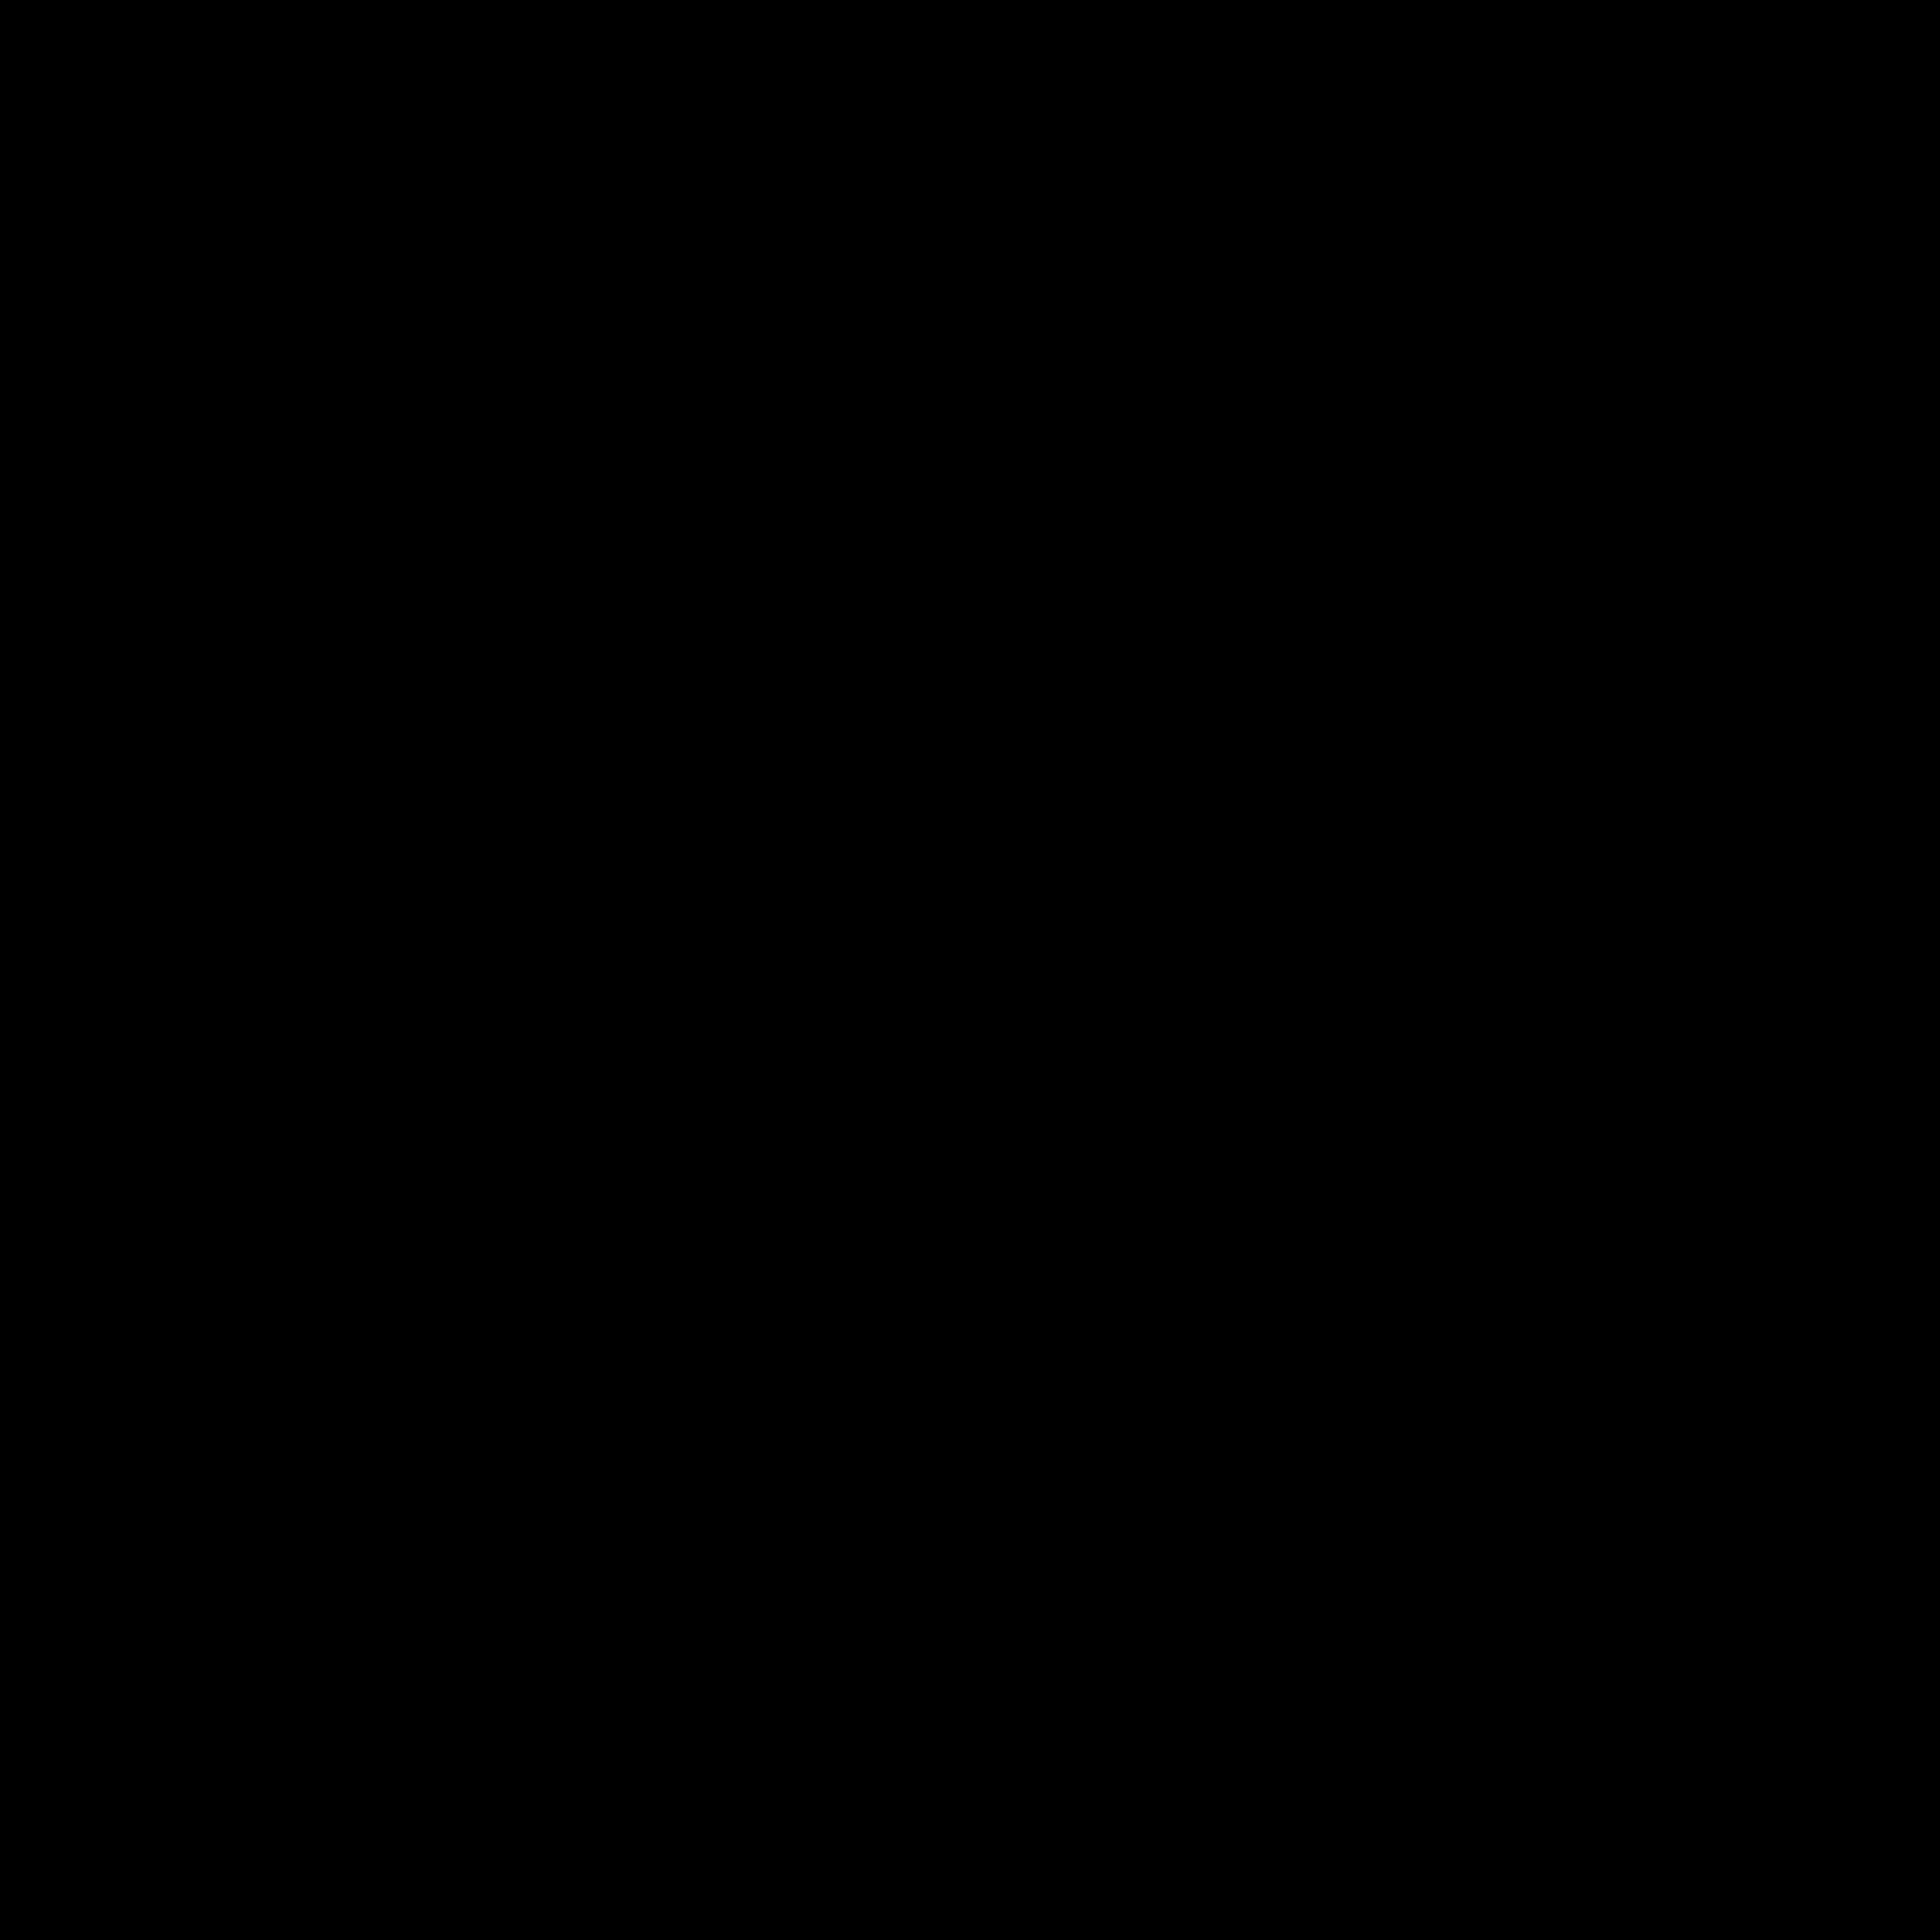
\includegraphics[width=\linewidth]{images/dense}
\caption{dense}
\end{subfigure}~%
\begin{subfigure}{\linewidth}
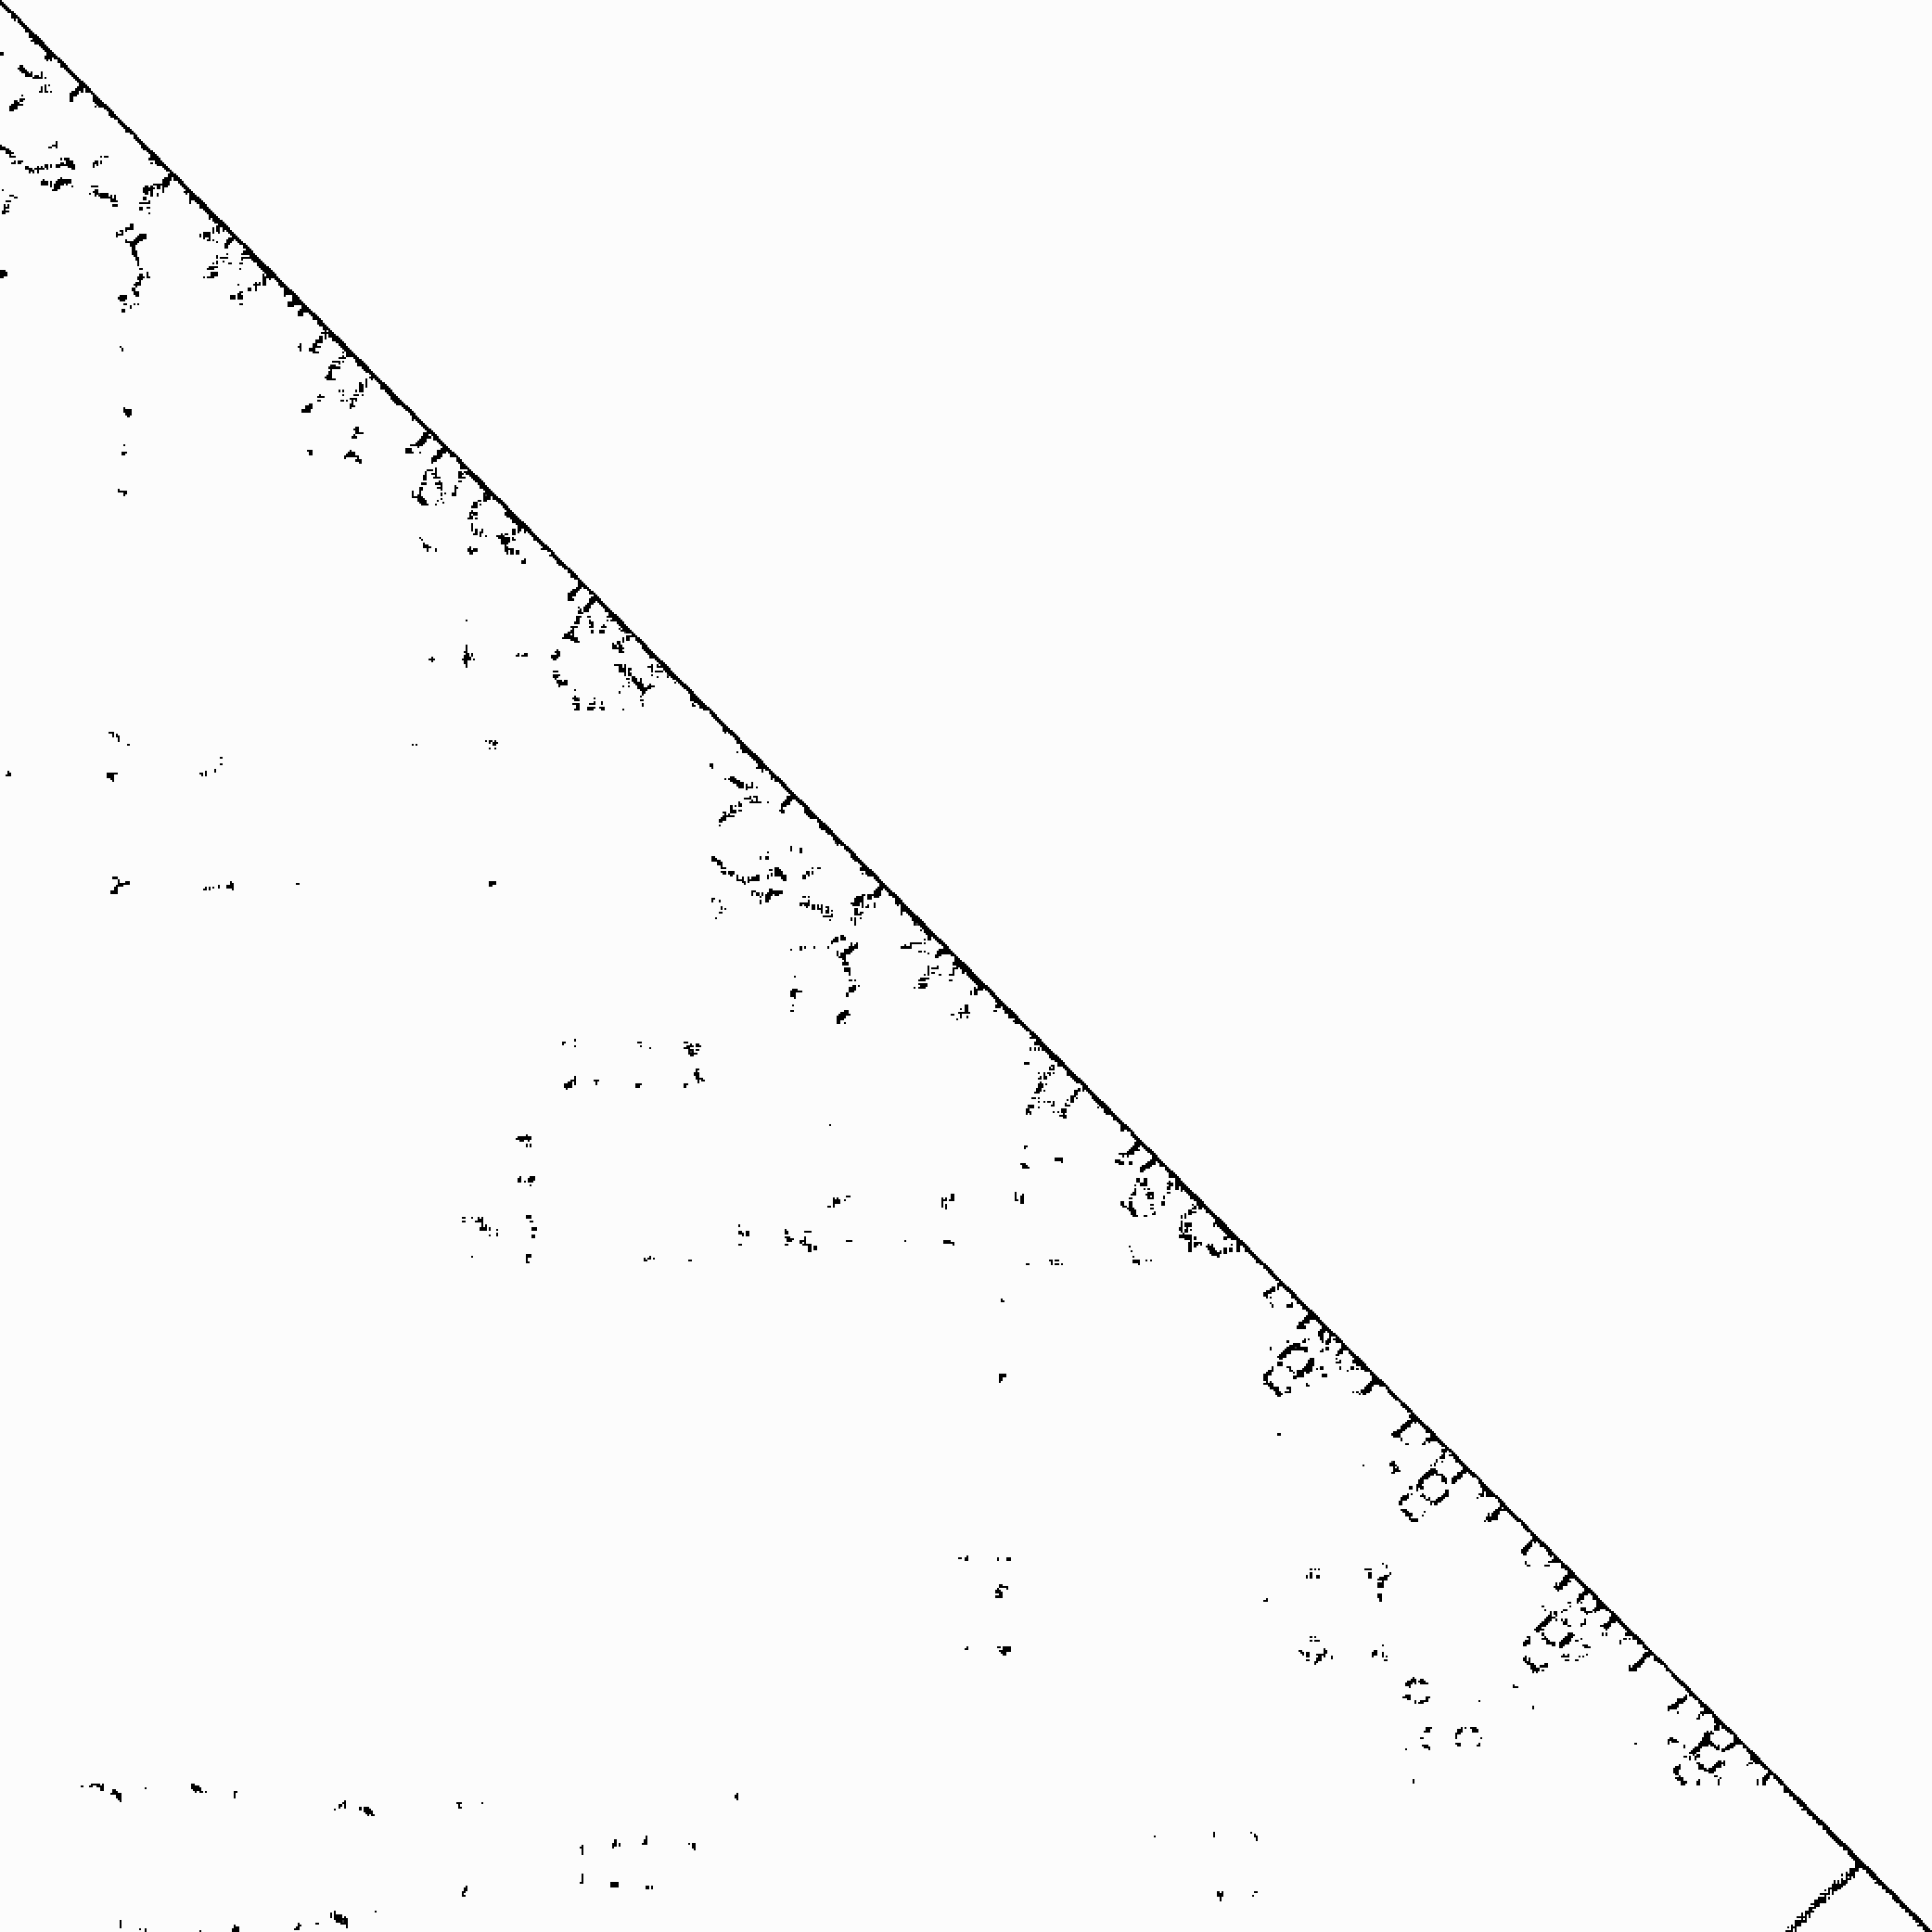
\includegraphics[width=\linewidth]{images/pdb1HYS}
\caption{pdb1HYS}
\end{subfigure}~%
\begin{subfigure}{\linewidth}
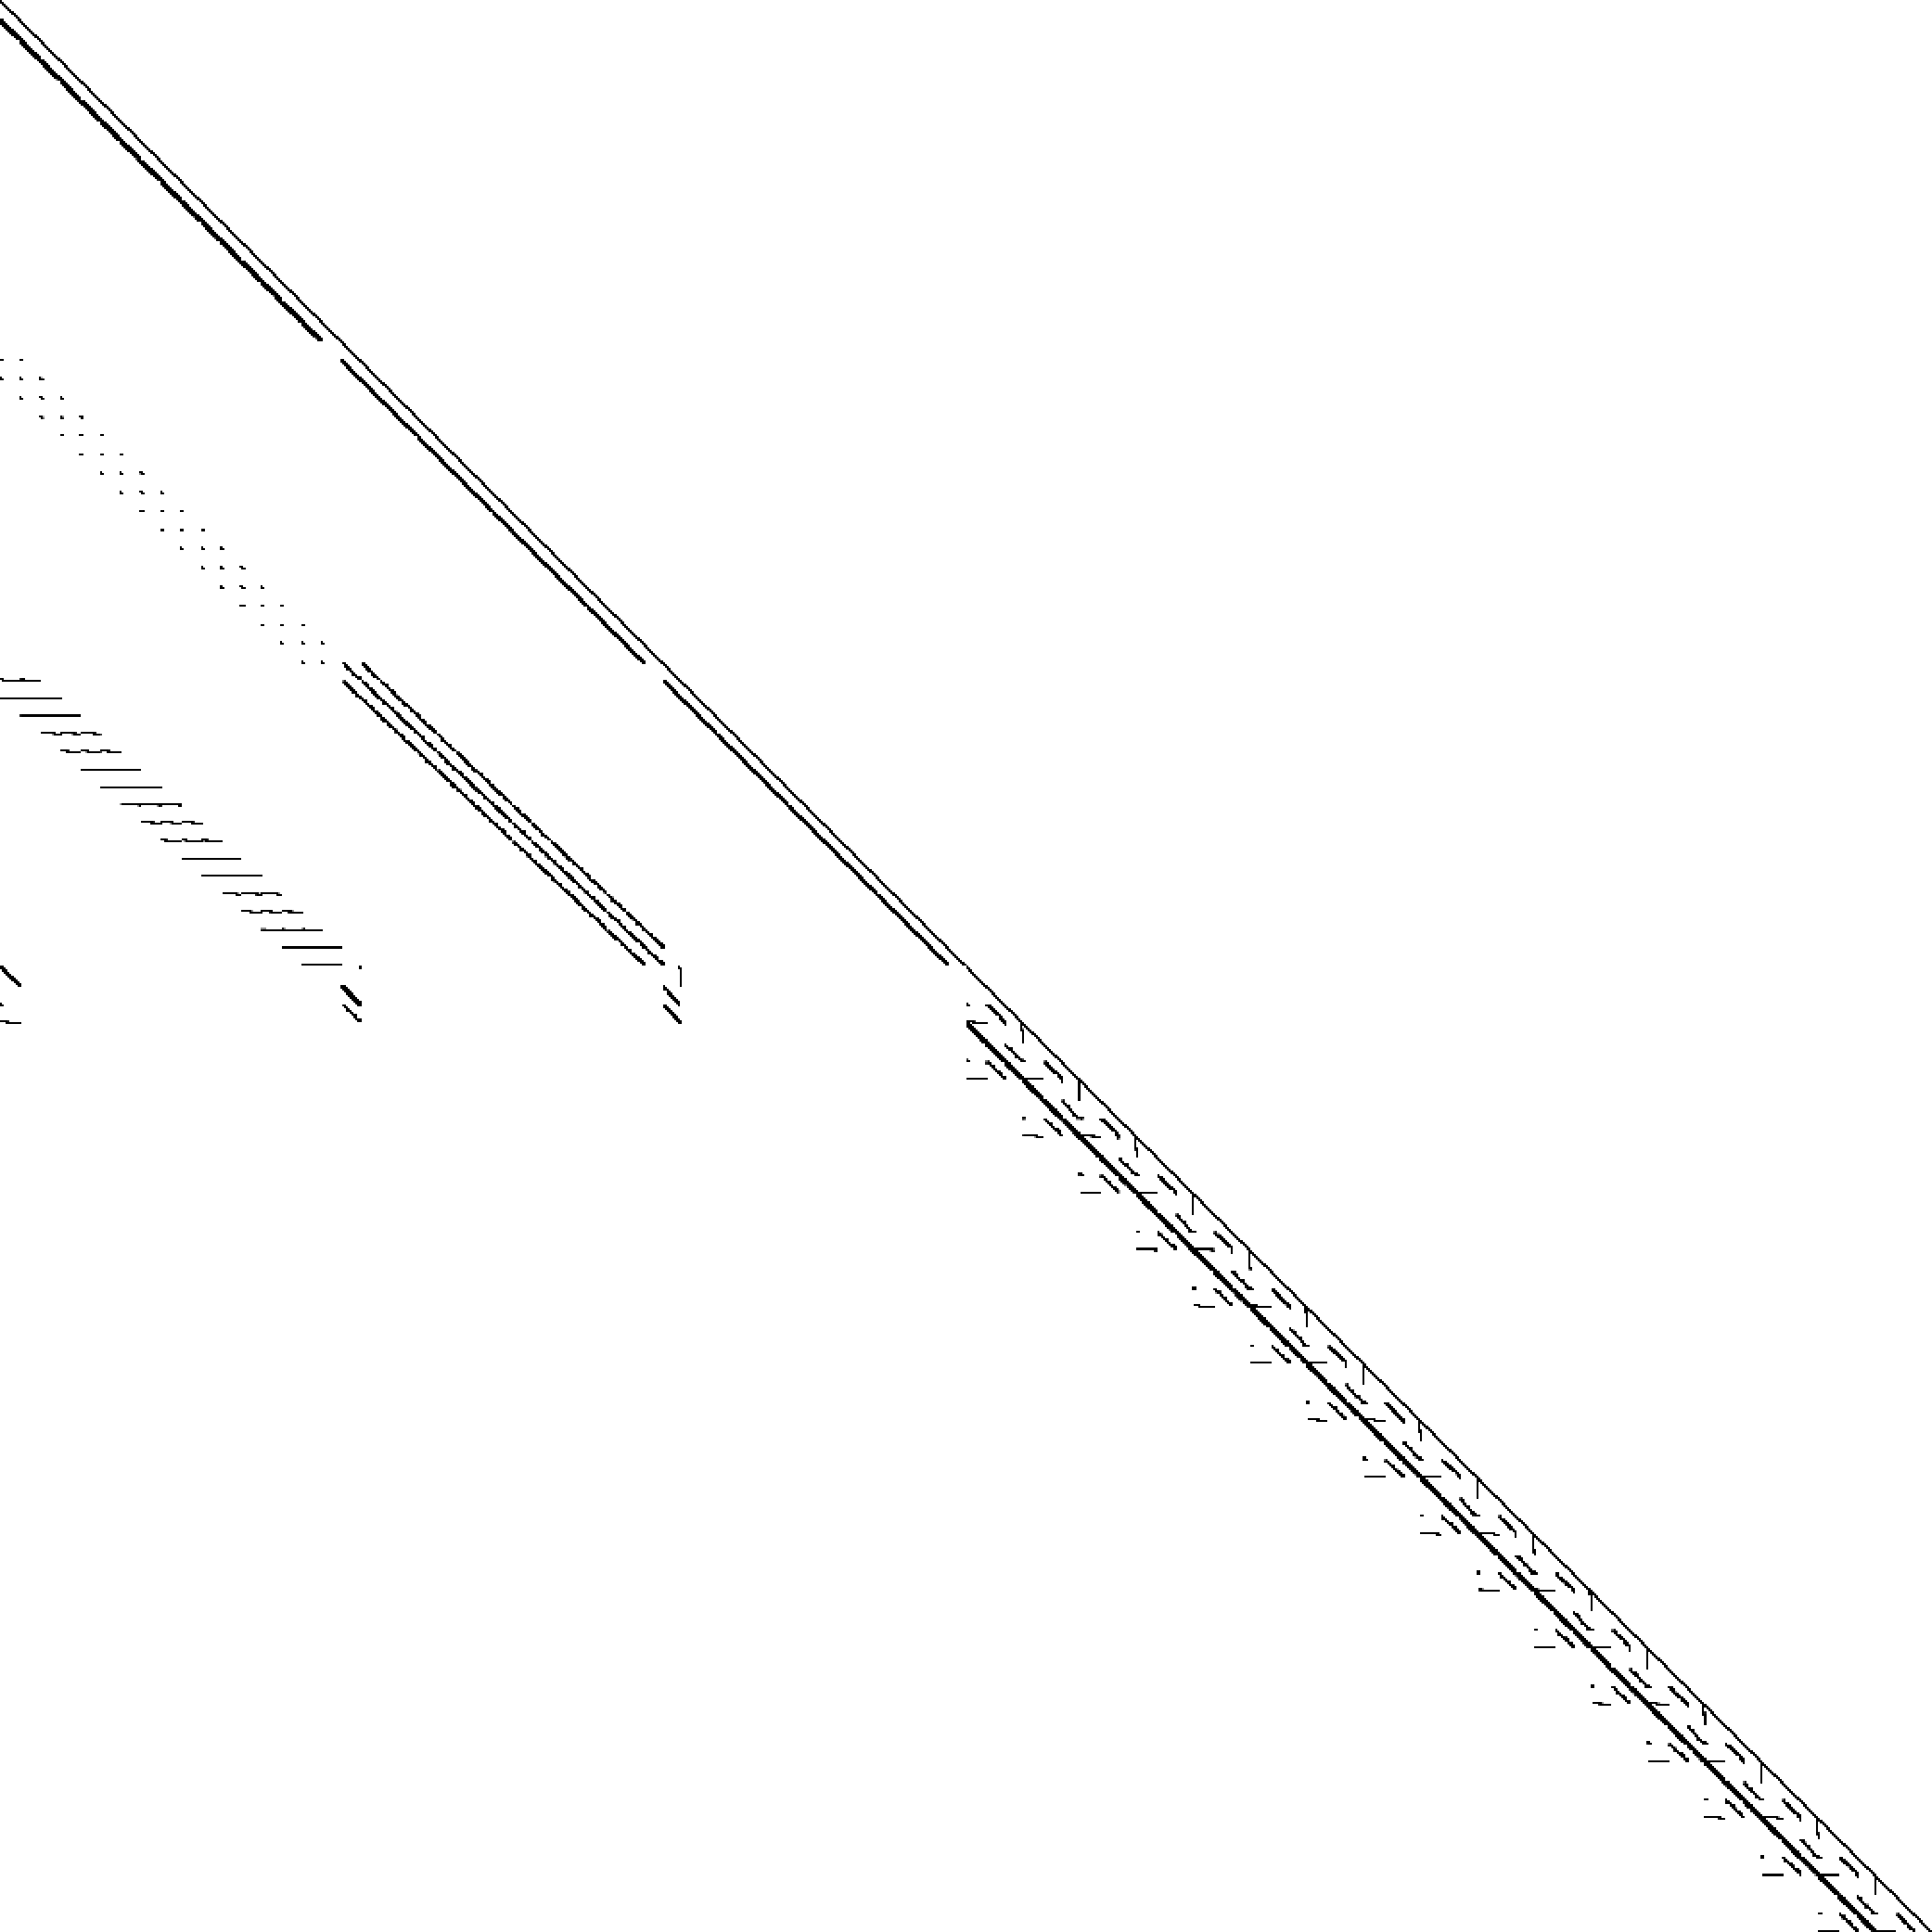
\includegraphics[width=\linewidth]{images/consph}
\caption{consph}
\end{subfigure}~%
\end{multicols}
%\begin{multicols}{3}
%\begin{subfigure}{\linewidth}
%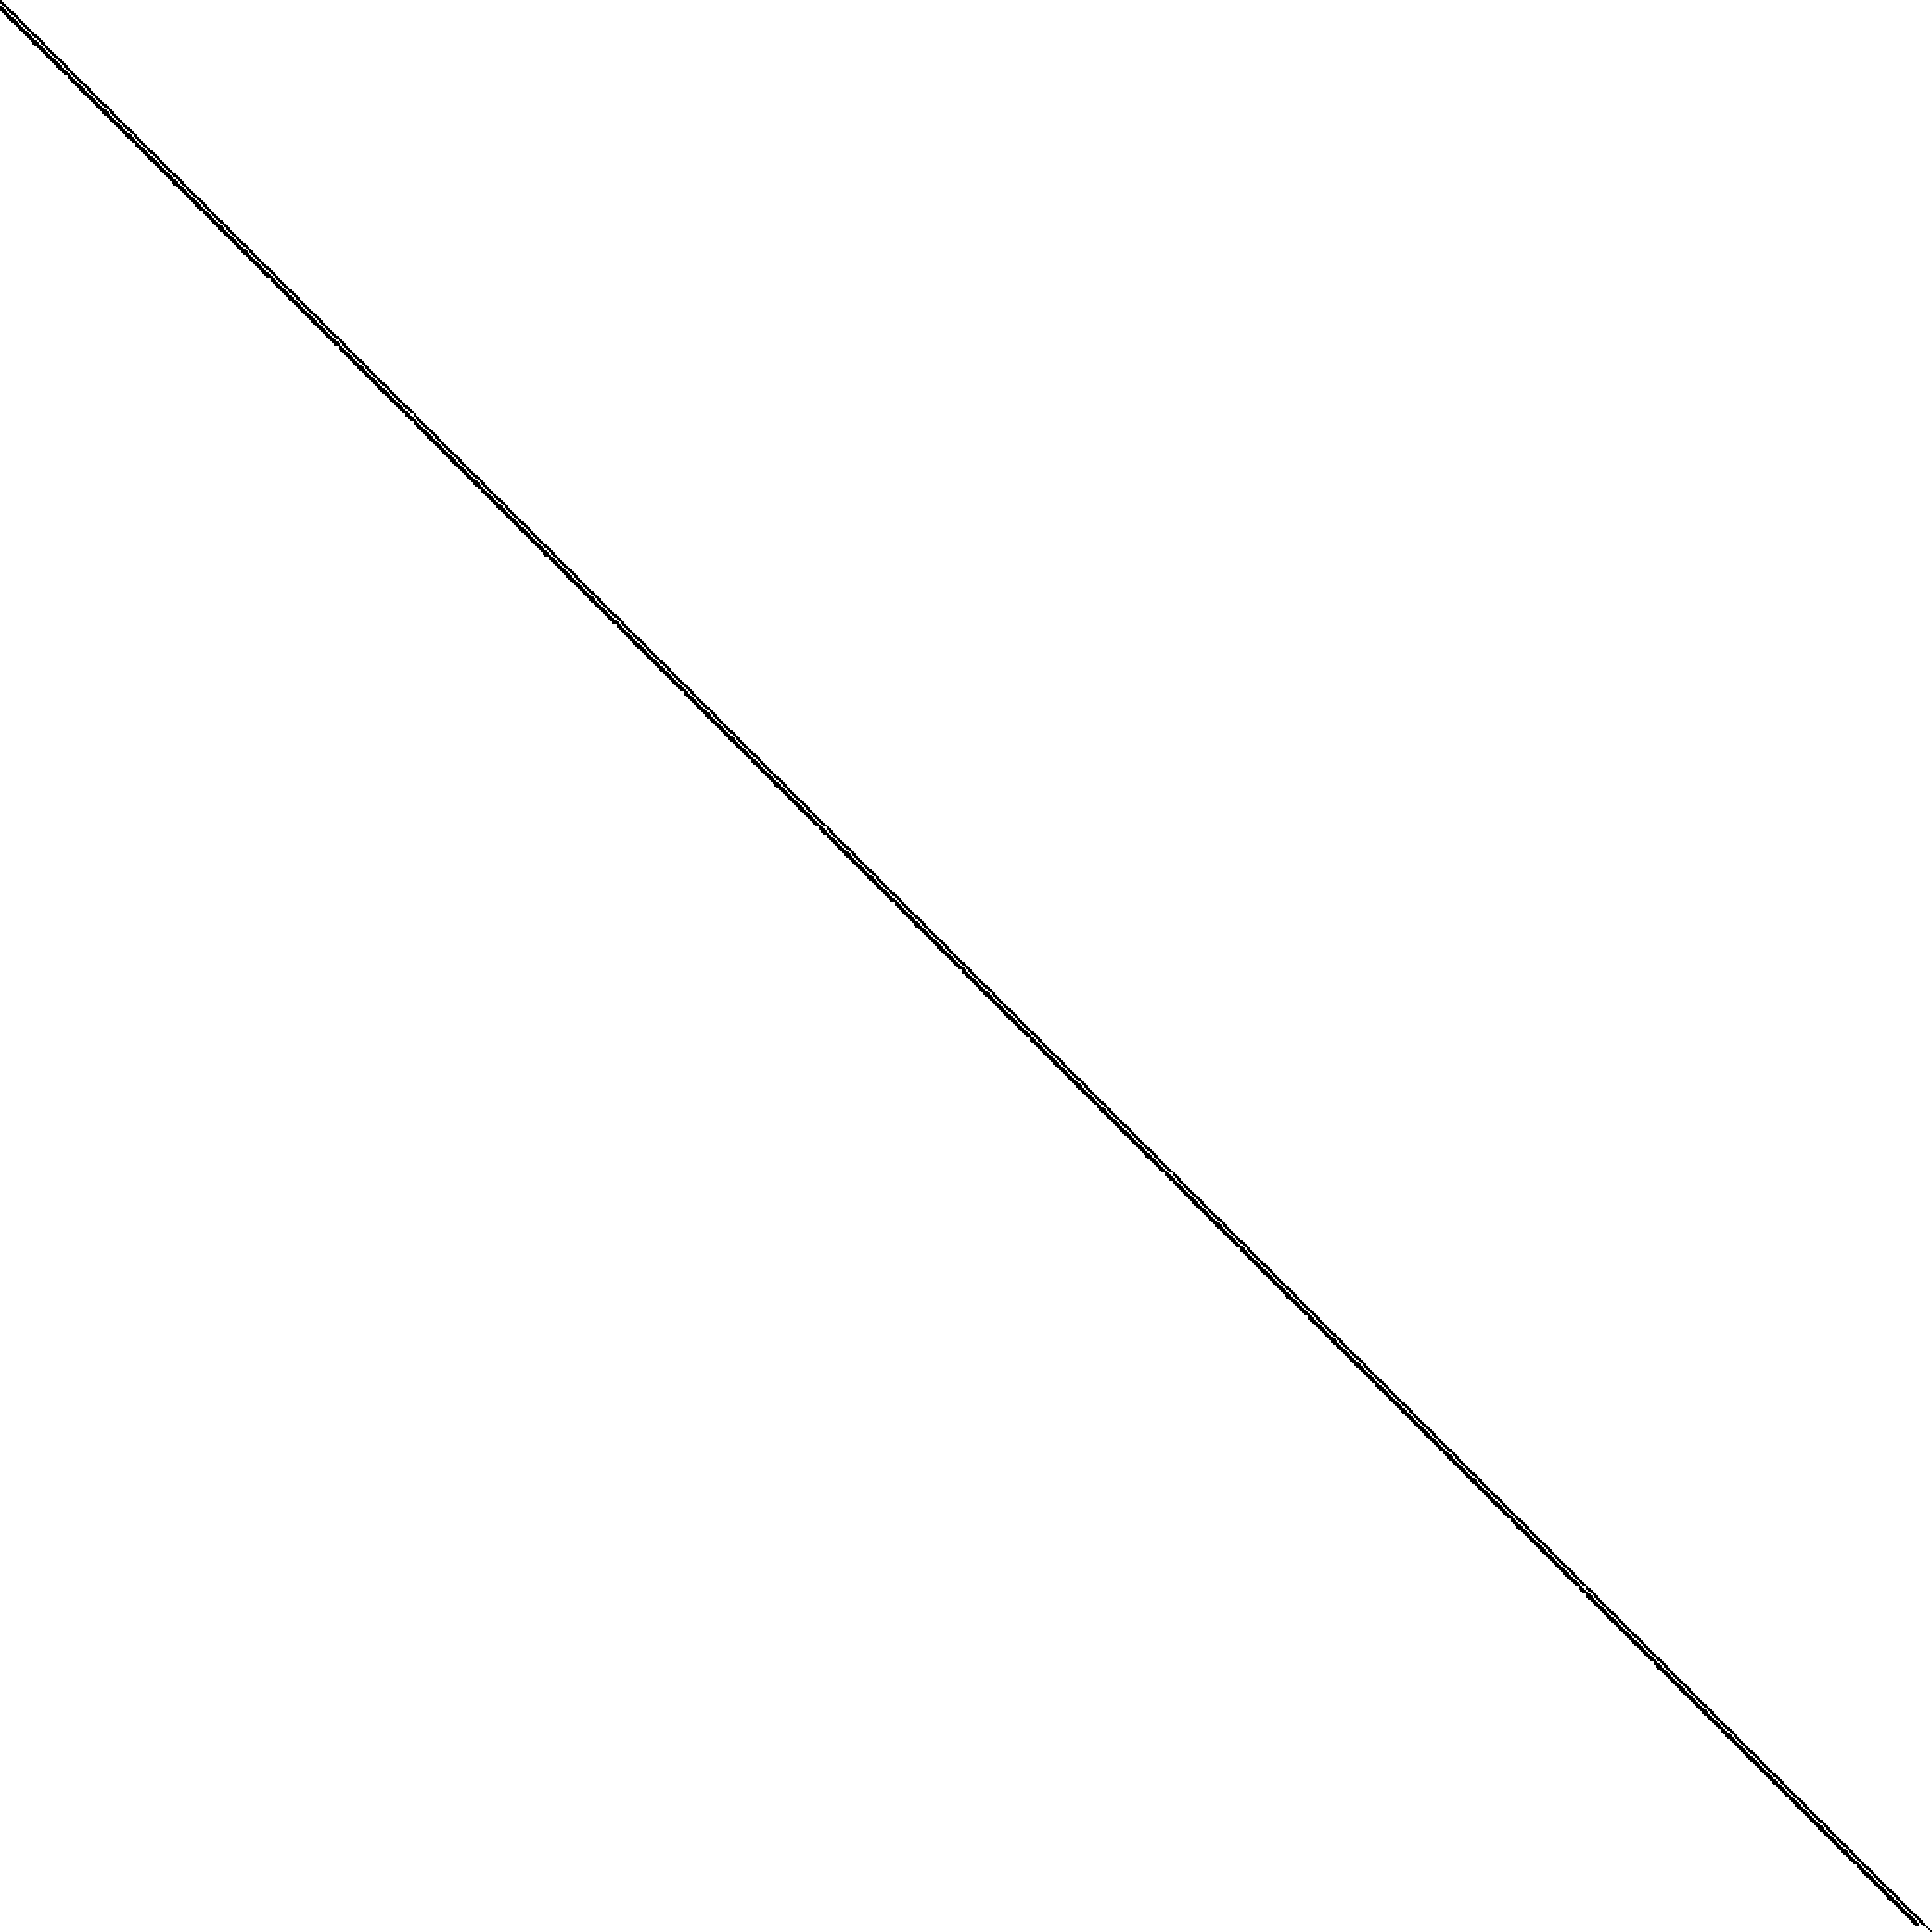
\includegraphics[width=\linewidth]{images/cant}
%\caption{cant}
%\end{subfigure}~%
%\begin{subfigure}{\linewidth}
%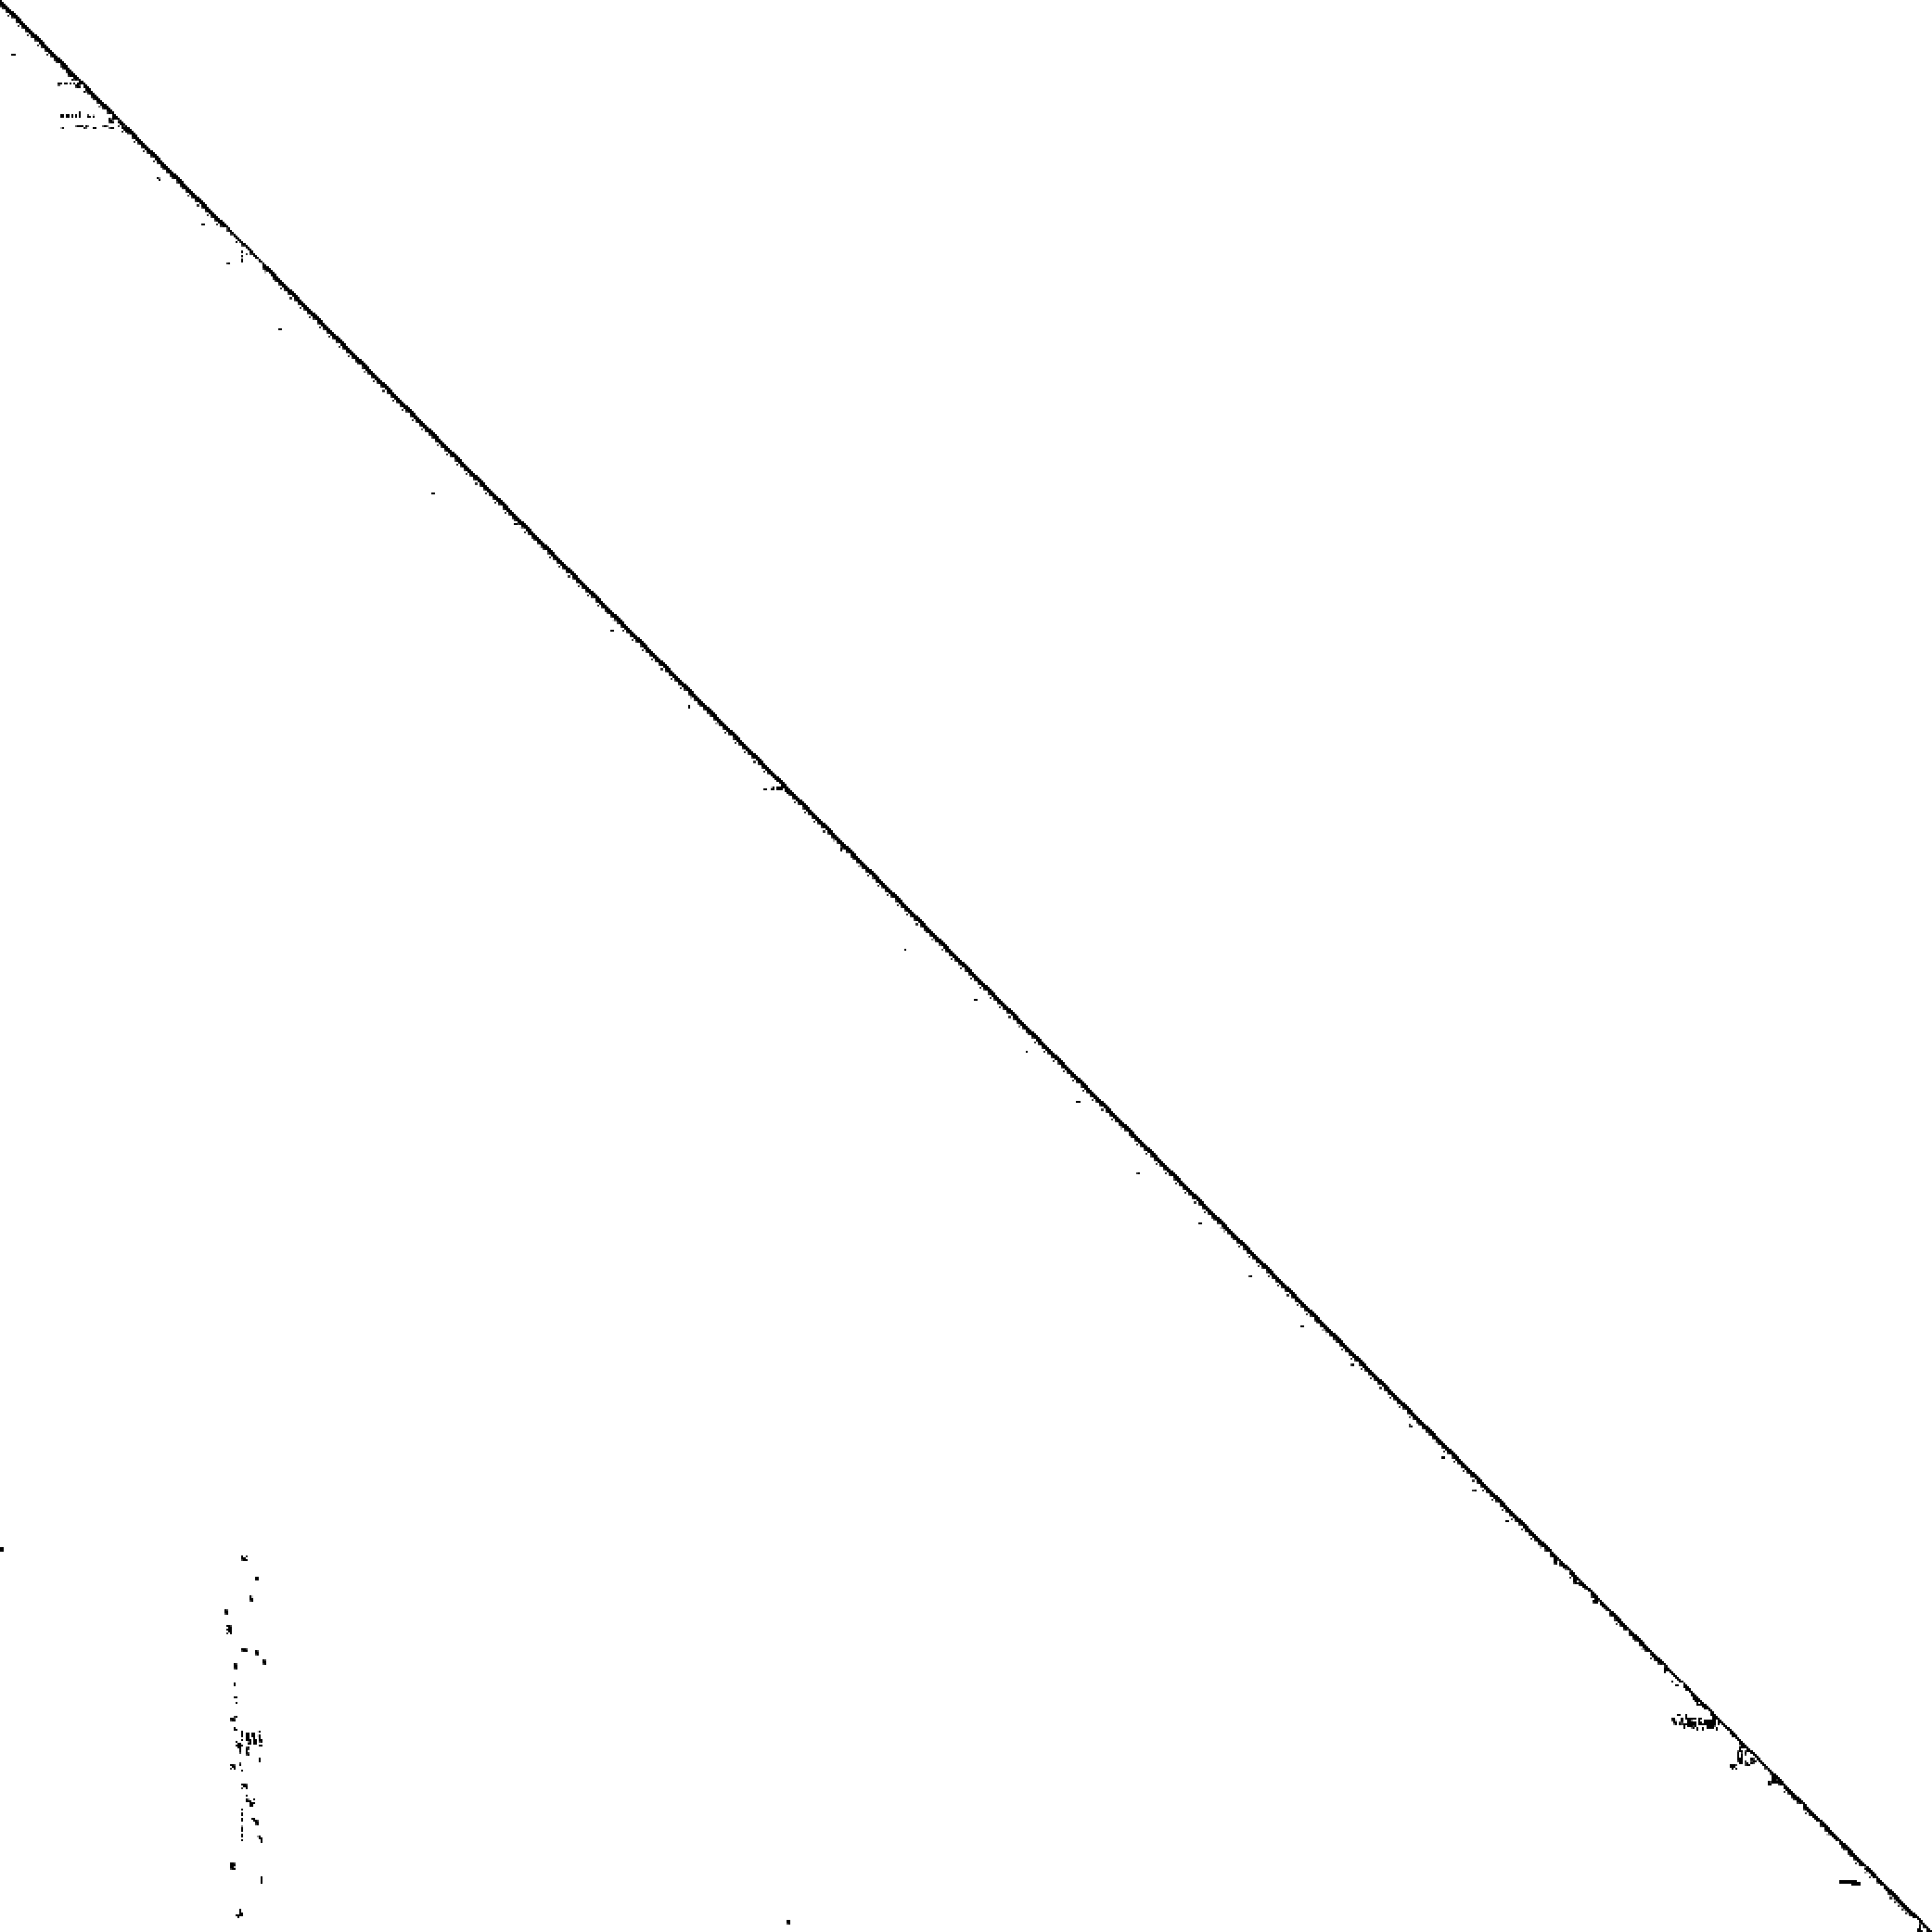
\includegraphics[width=\linewidth]{images/pwtk}
%\caption{pwtk}
%\end{subfigure}~%
%\begin{subfigure}{\linewidth}
%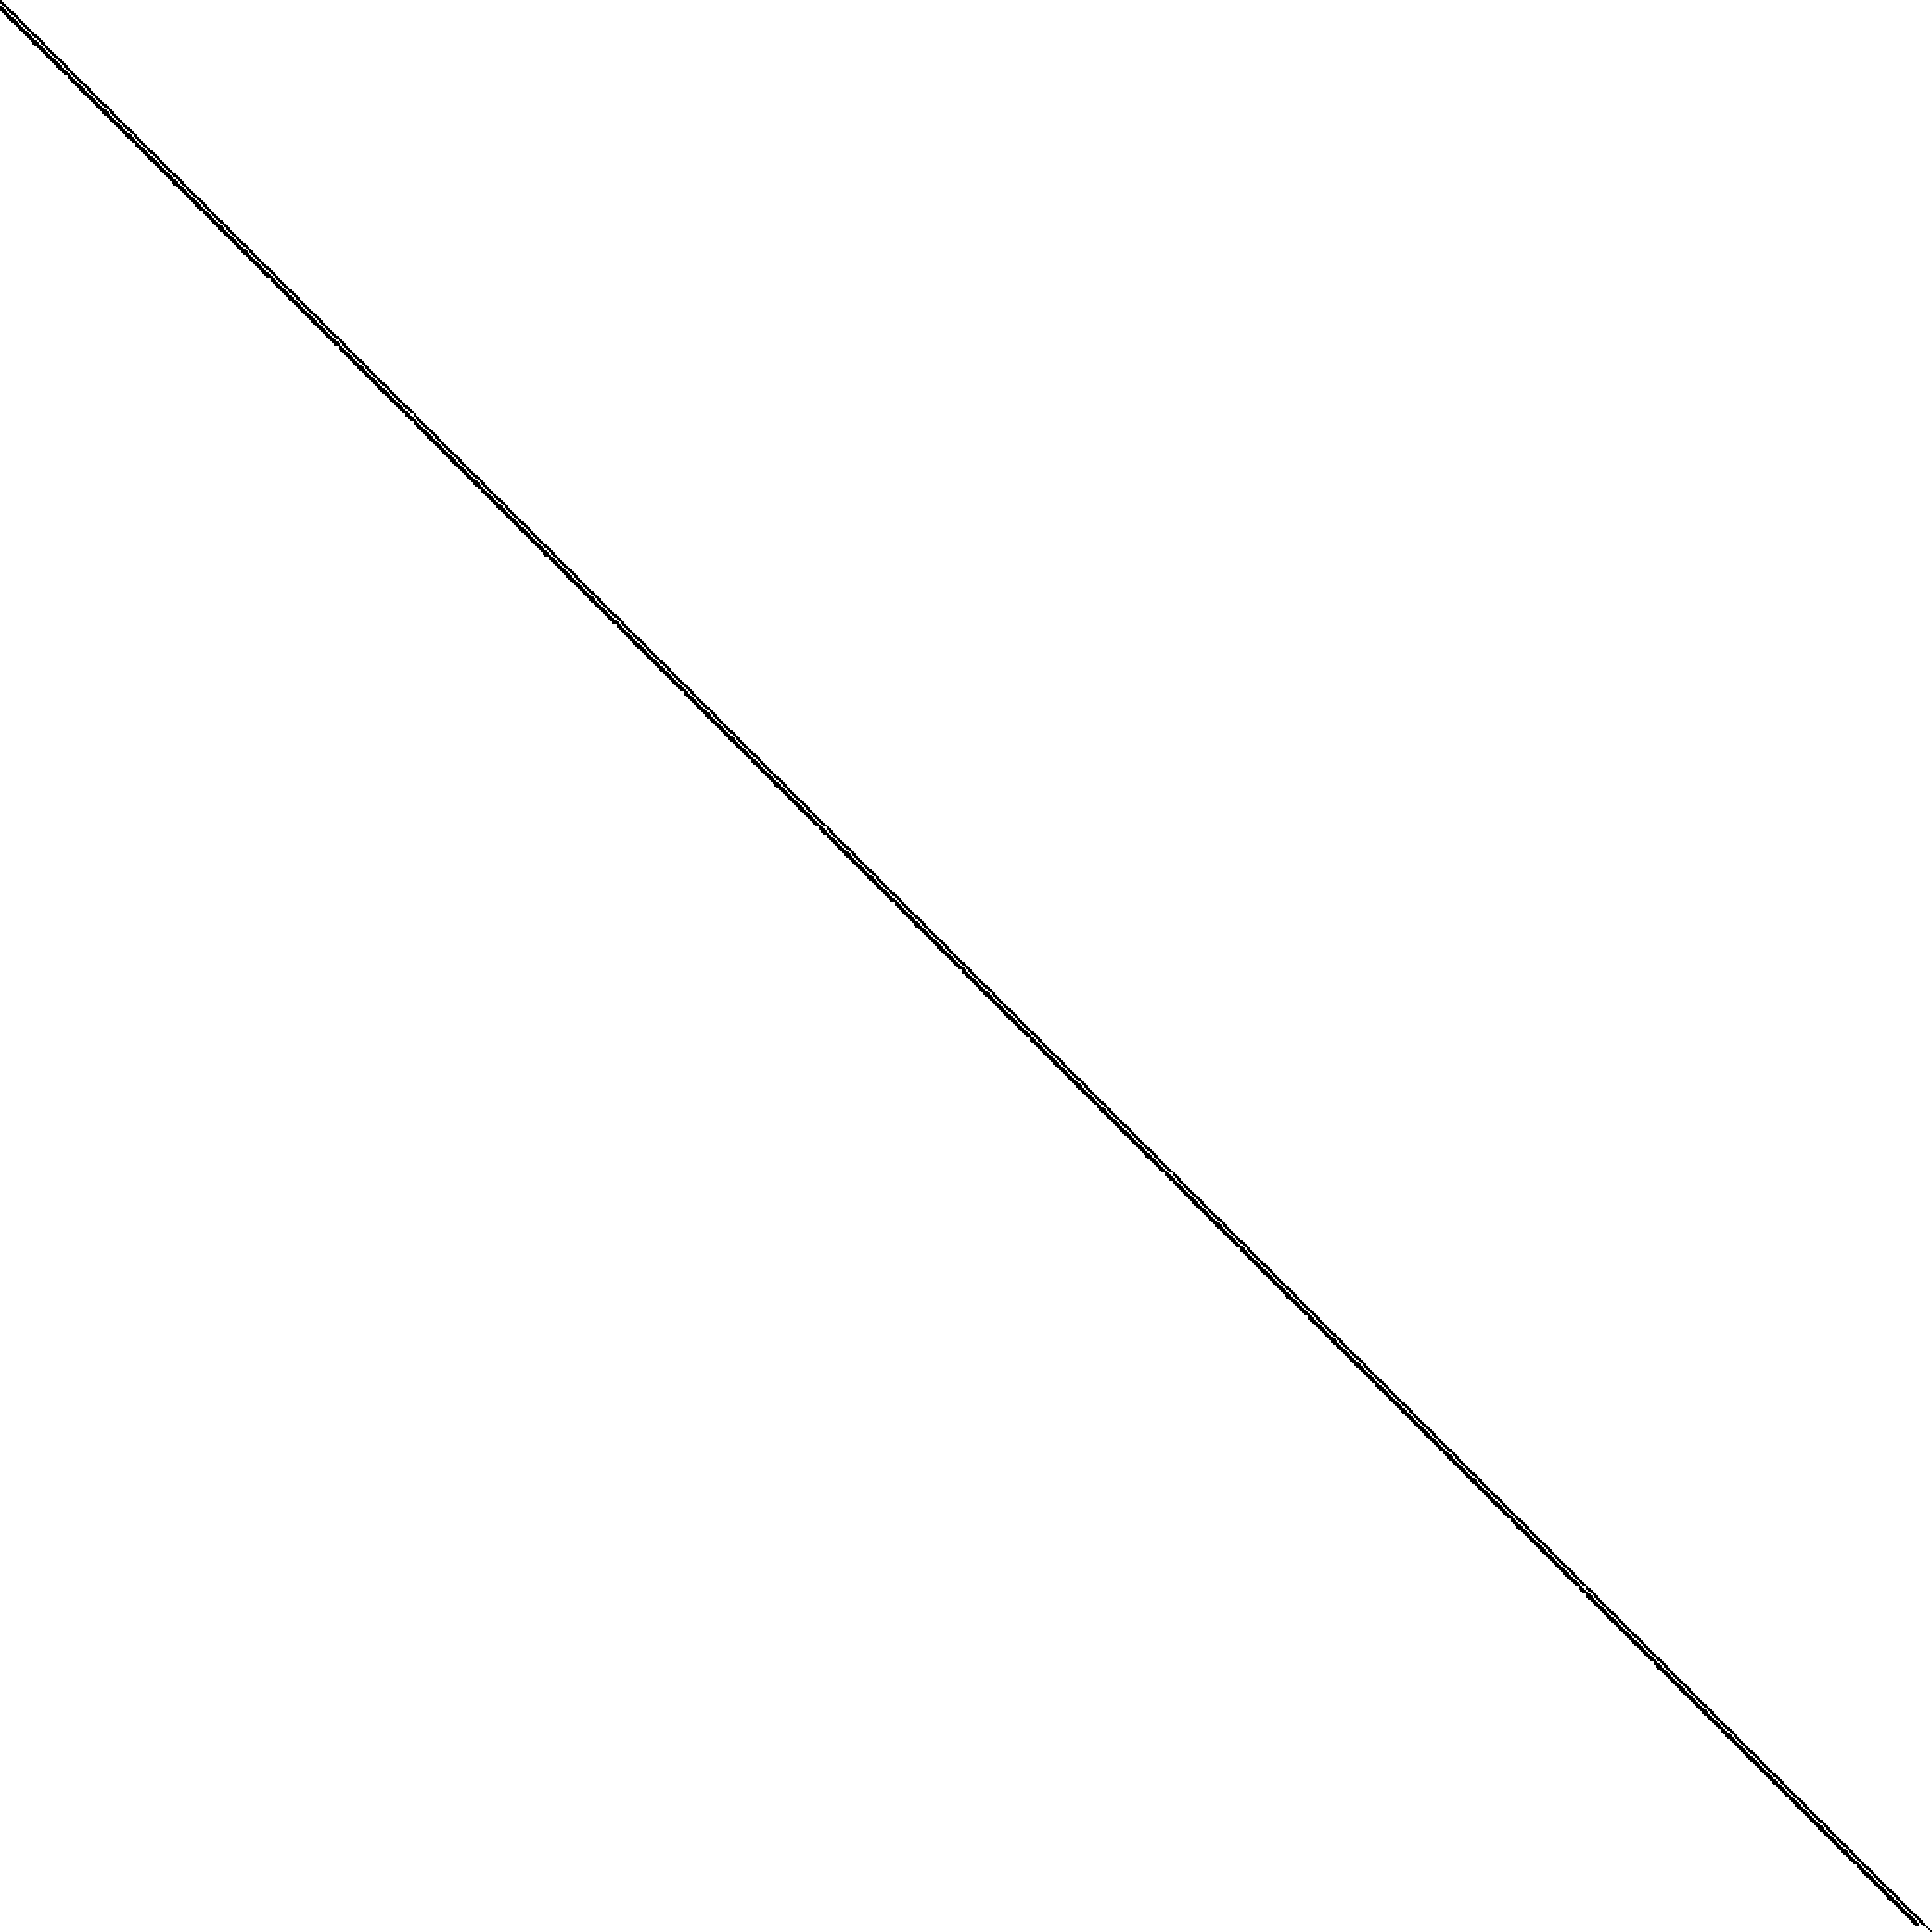
\includegraphics[width=\linewidth]{images/cant}
%\caption{cant}
%\end{subfigure}~%
%\end{multicols}
\begin{multicols}{3}
\begin{subfigure}{\linewidth}
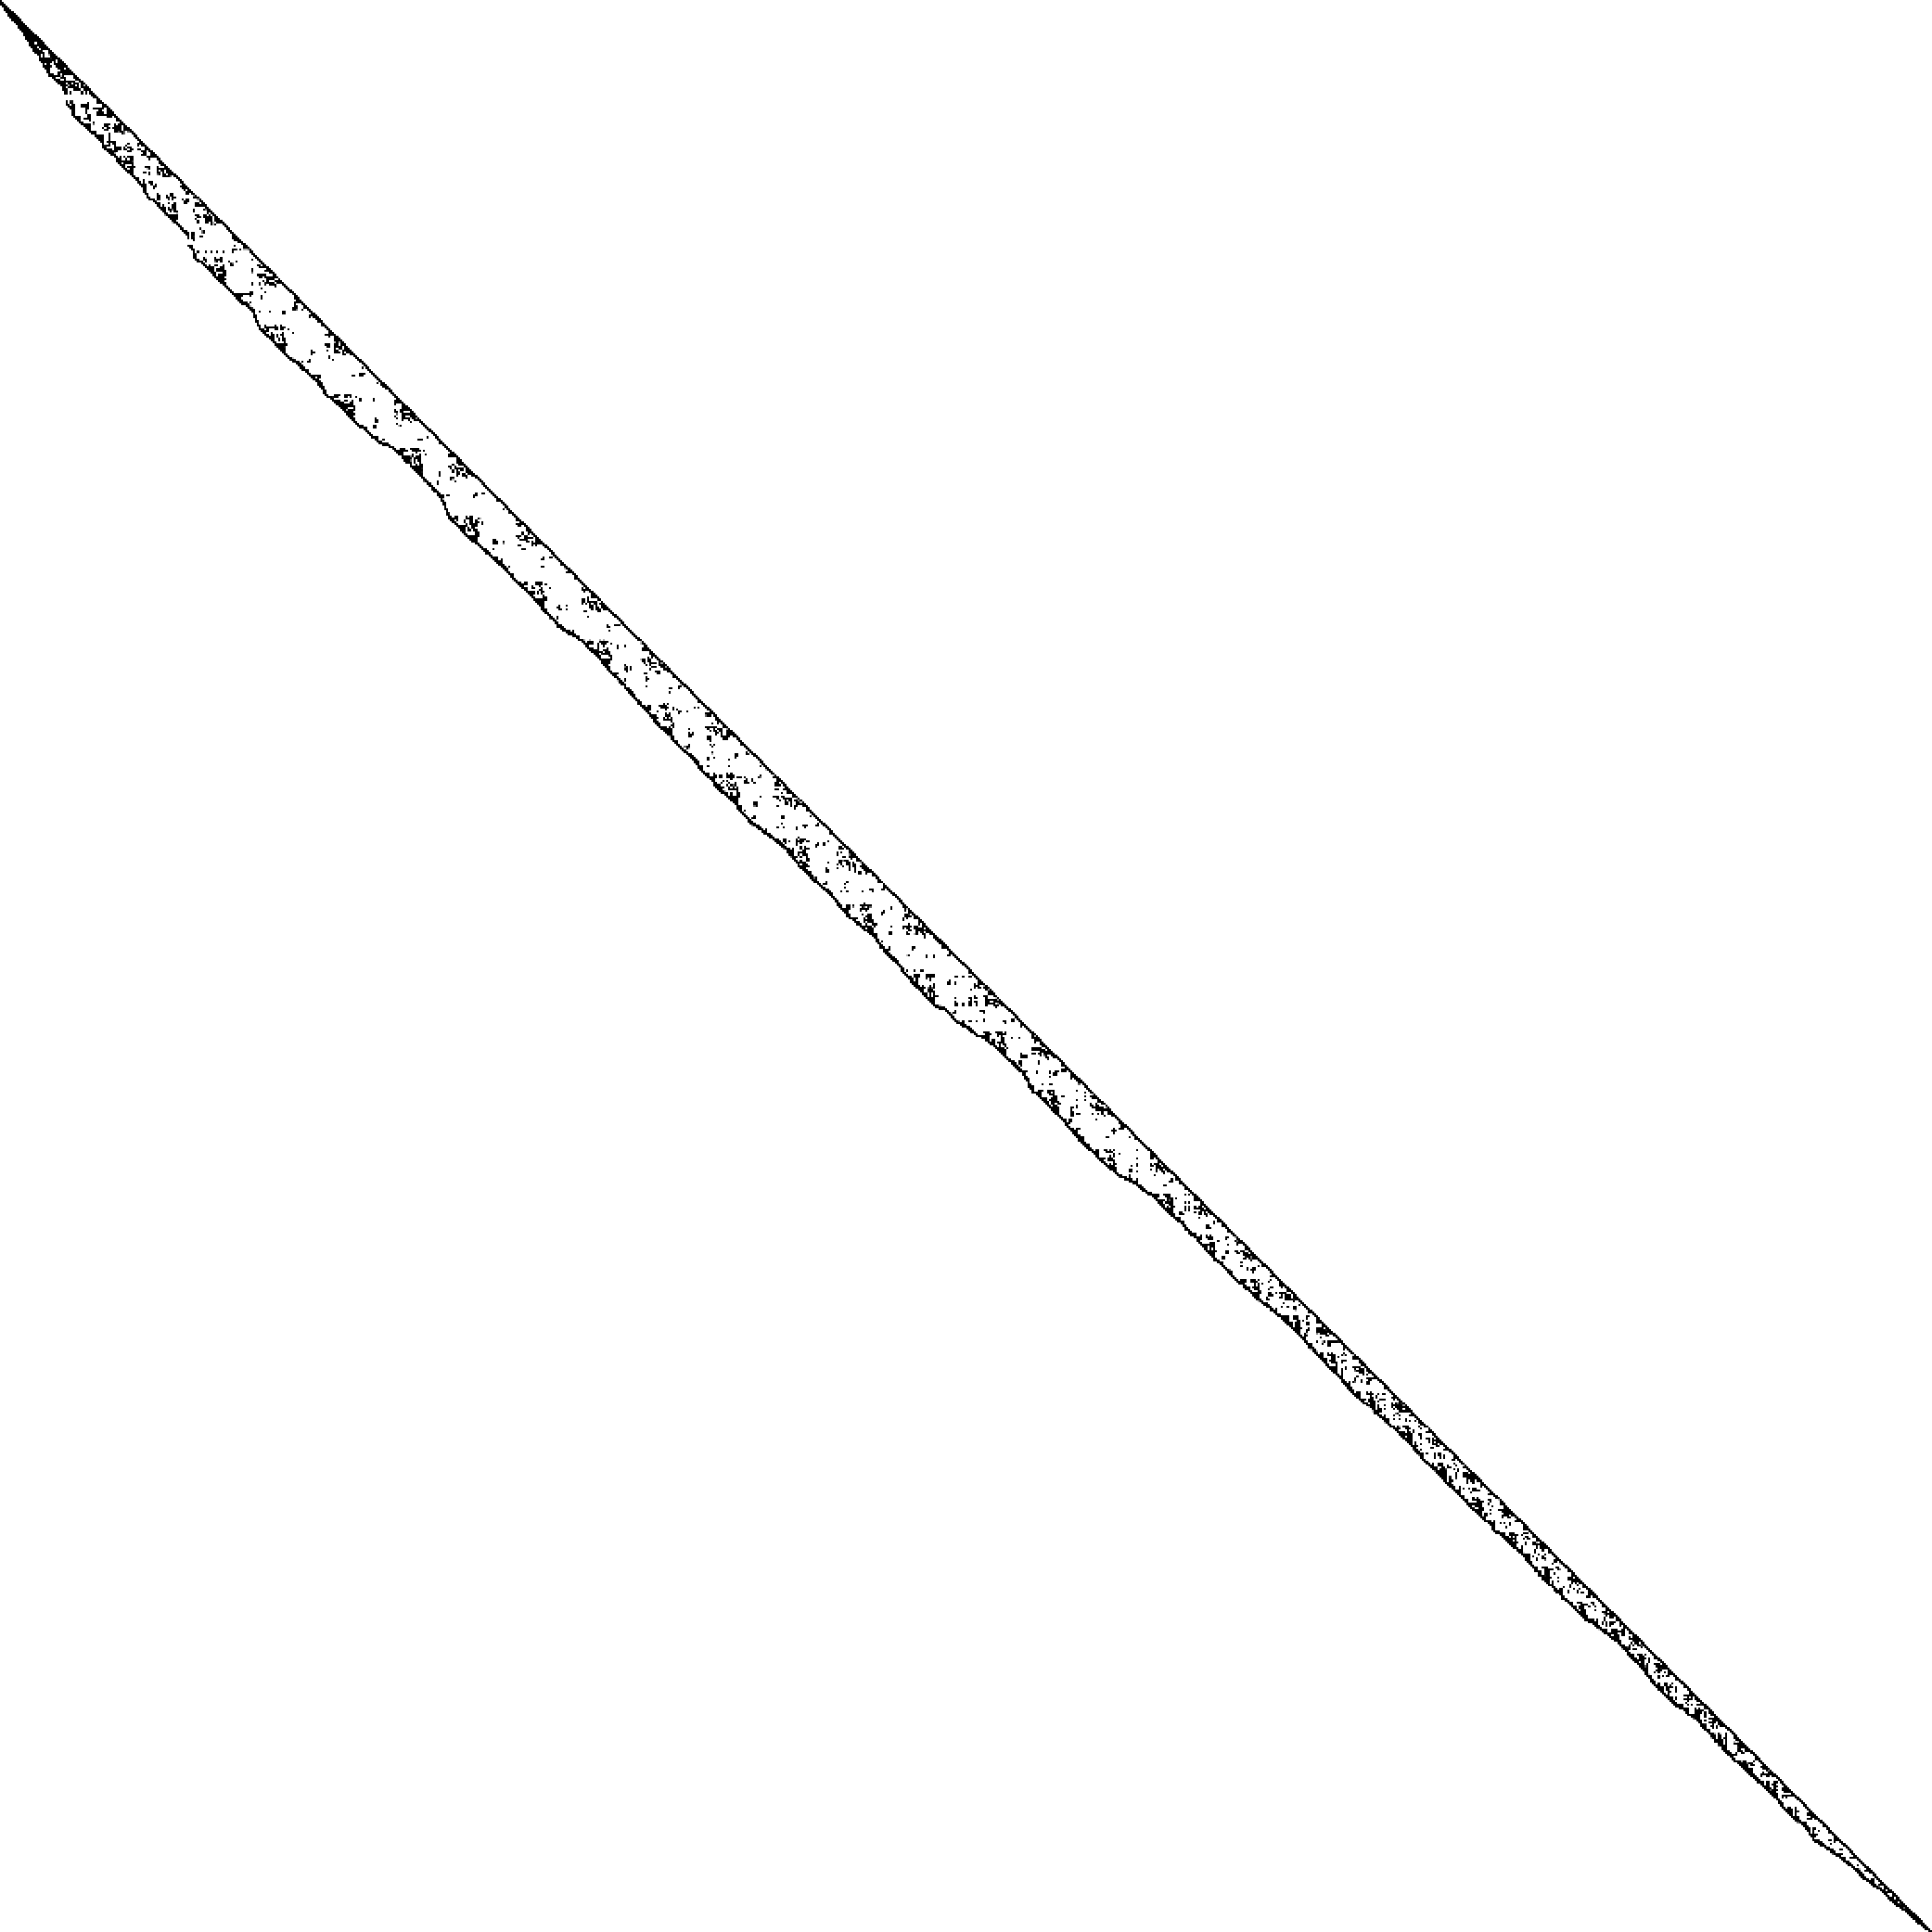
\includegraphics[width=\linewidth]{images/shipsec1}
\caption{shipsec1}
\end{subfigure}~%
\begin{subfigure}{\linewidth}
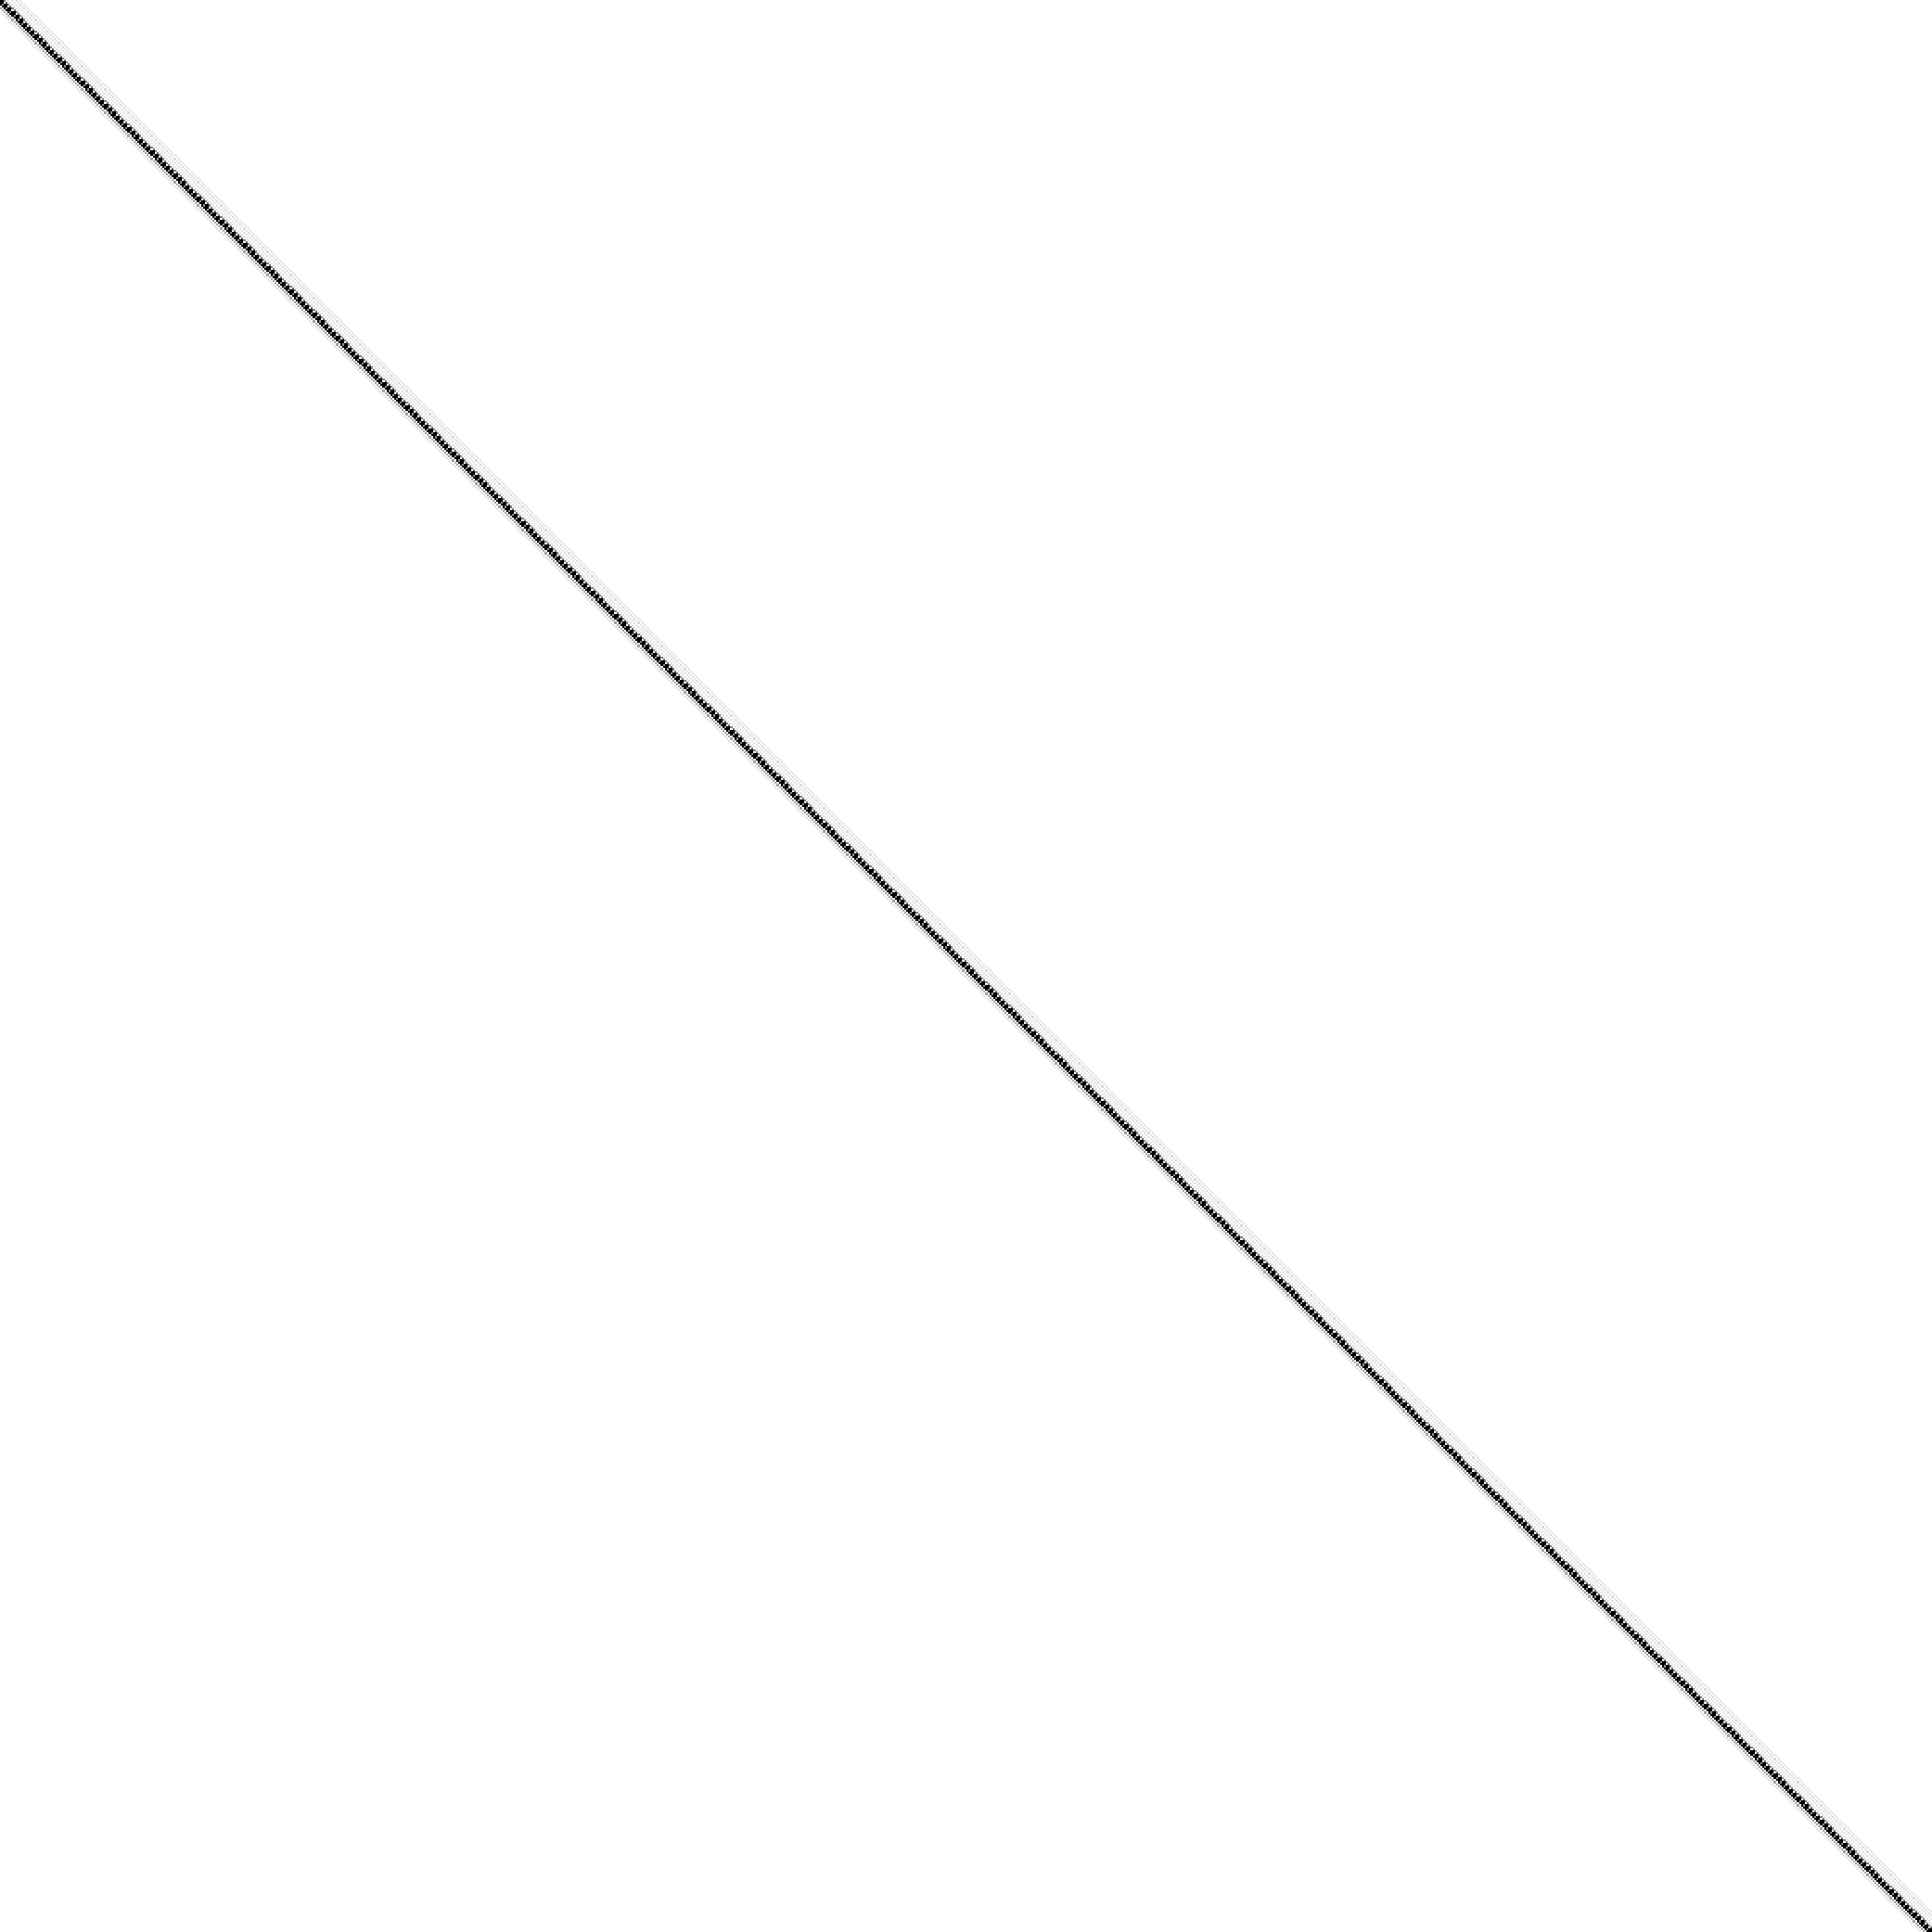
\includegraphics[width=\linewidth]{images/mac_econ_fwd500}
\caption{mac\_econ\_fwd500}
\end{subfigure}~%
\begin{subfigure}{\linewidth}
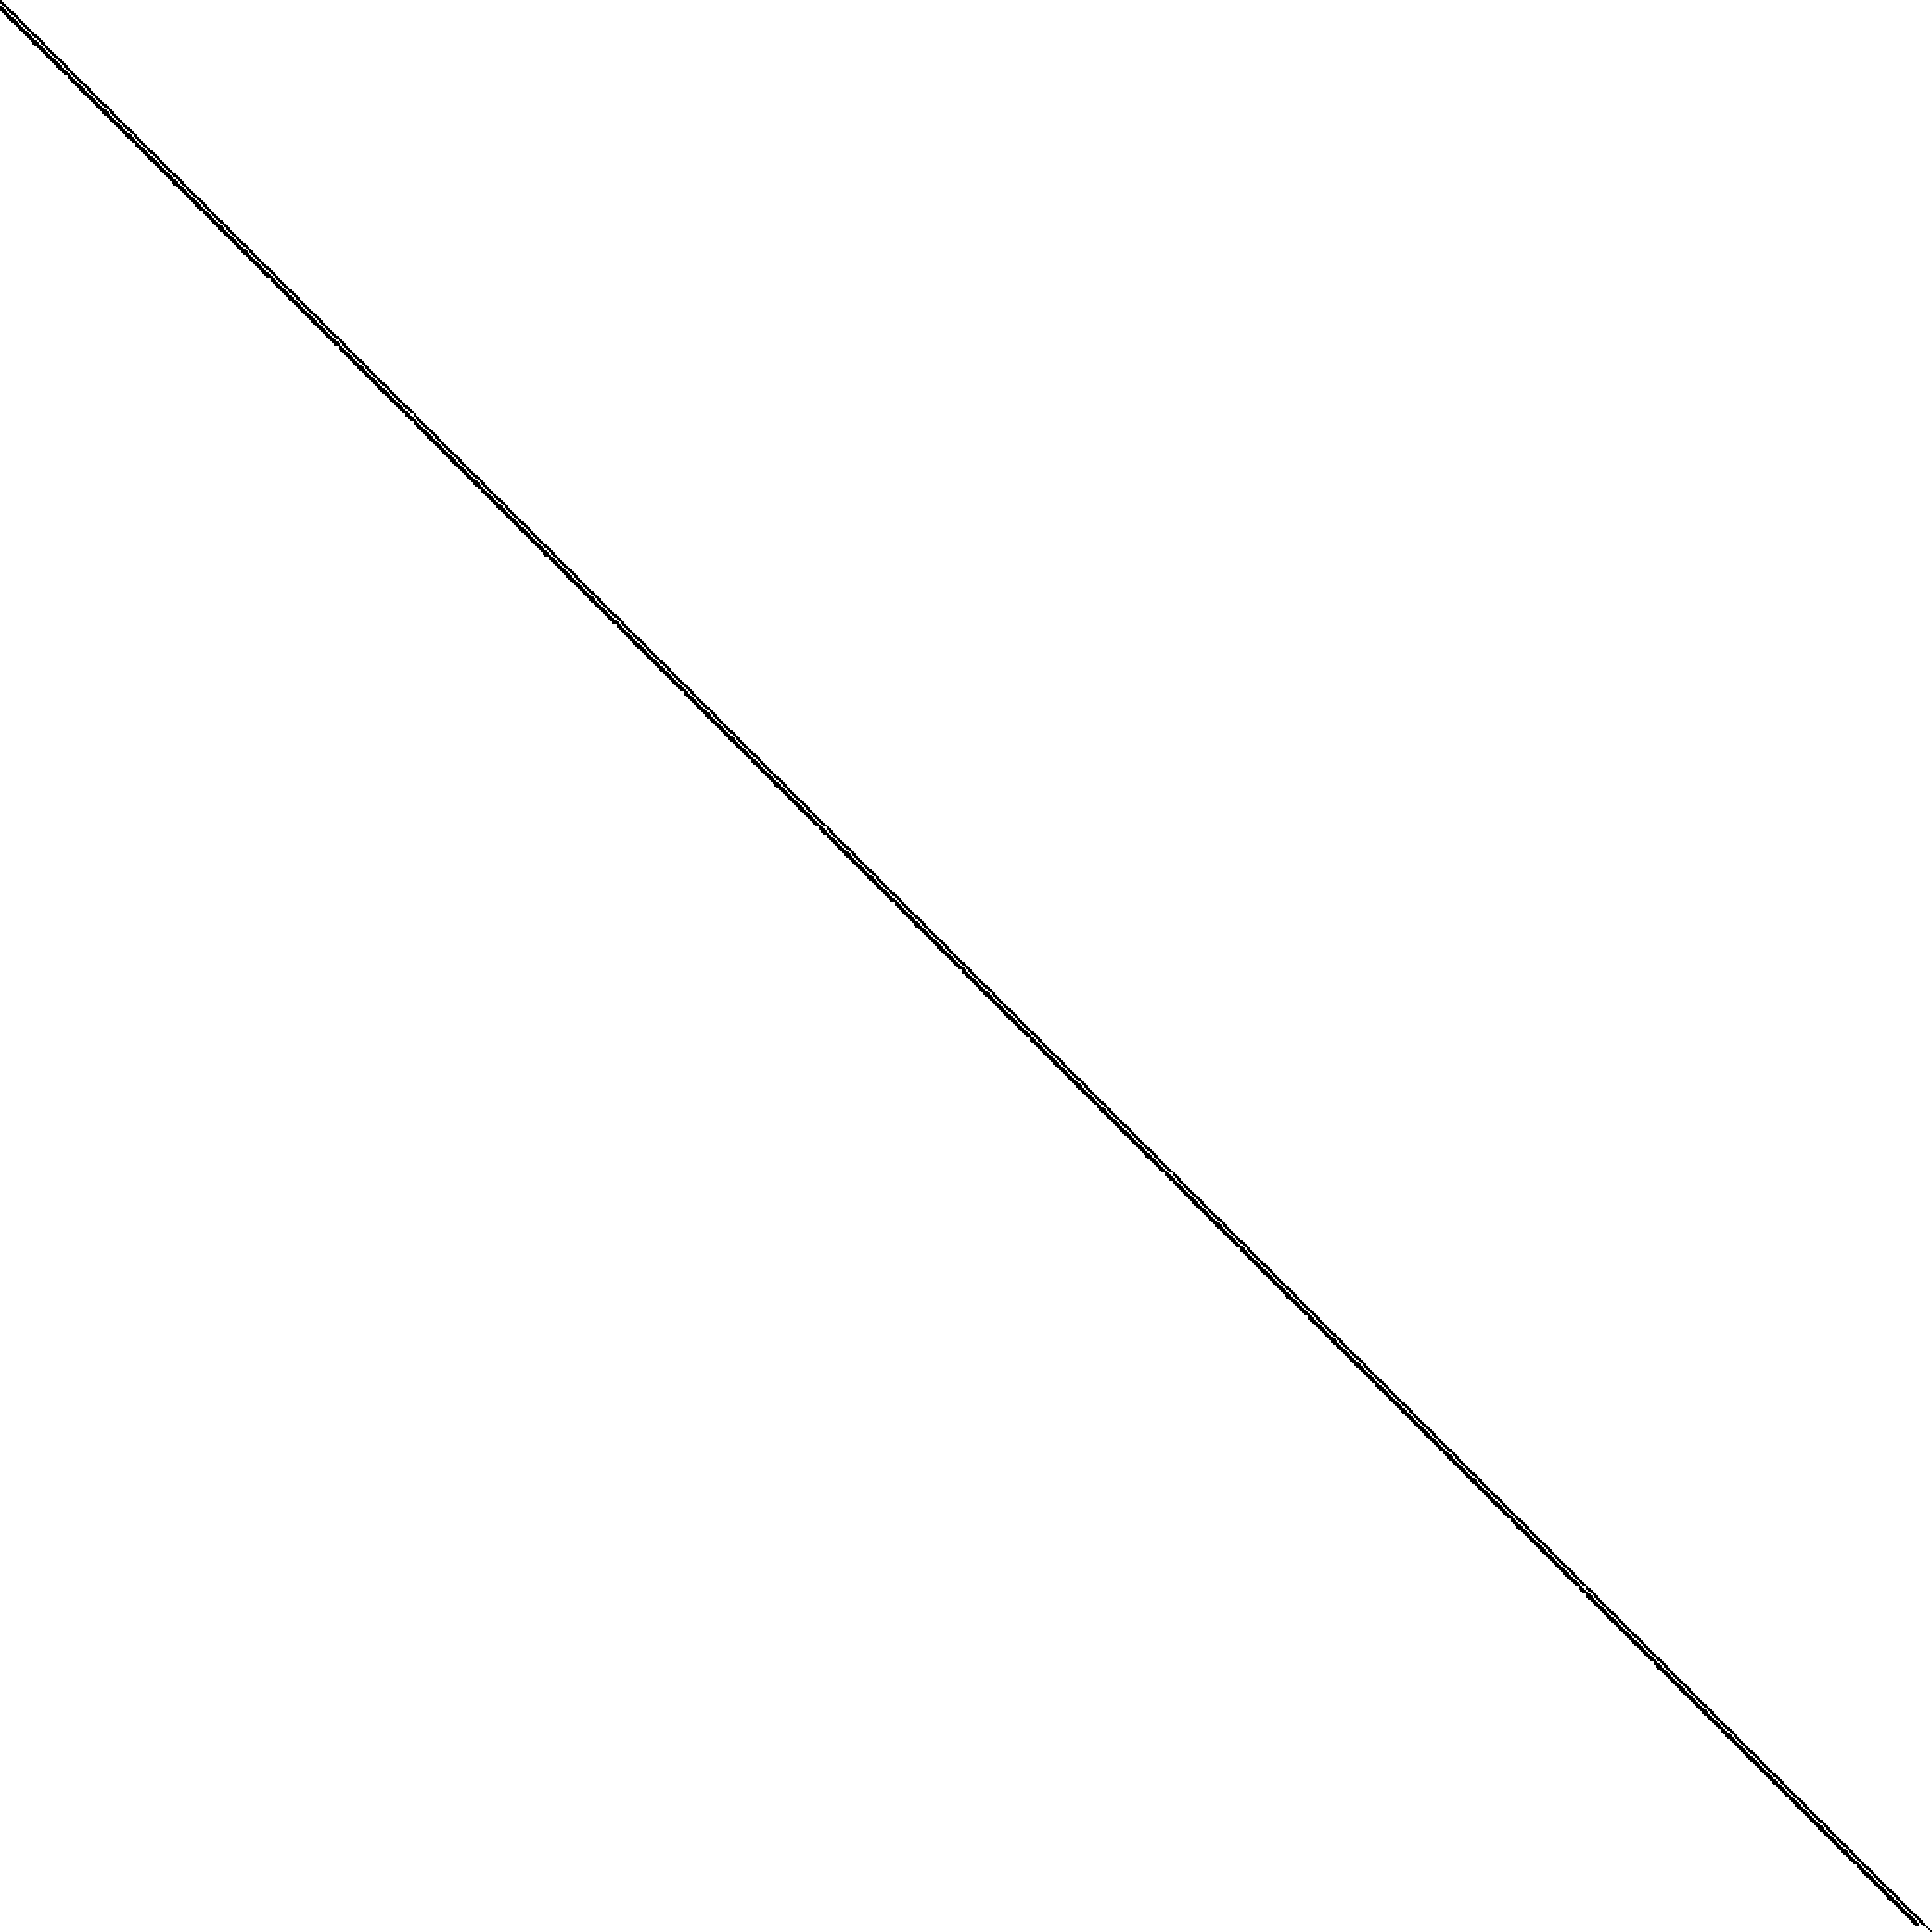
\includegraphics[width=\linewidth]{images/cant}
\caption{cant}
\end{subfigure}~%
\end{multicols}
\begin{multicols}{3}
\begin{subfigure}{\linewidth}

\includegraphics[width=\linewidth]{images/cop20k_A}
\caption{cop20k\_A}
\end{subfigure}~%
\begin{subfigure}{\linewidth}
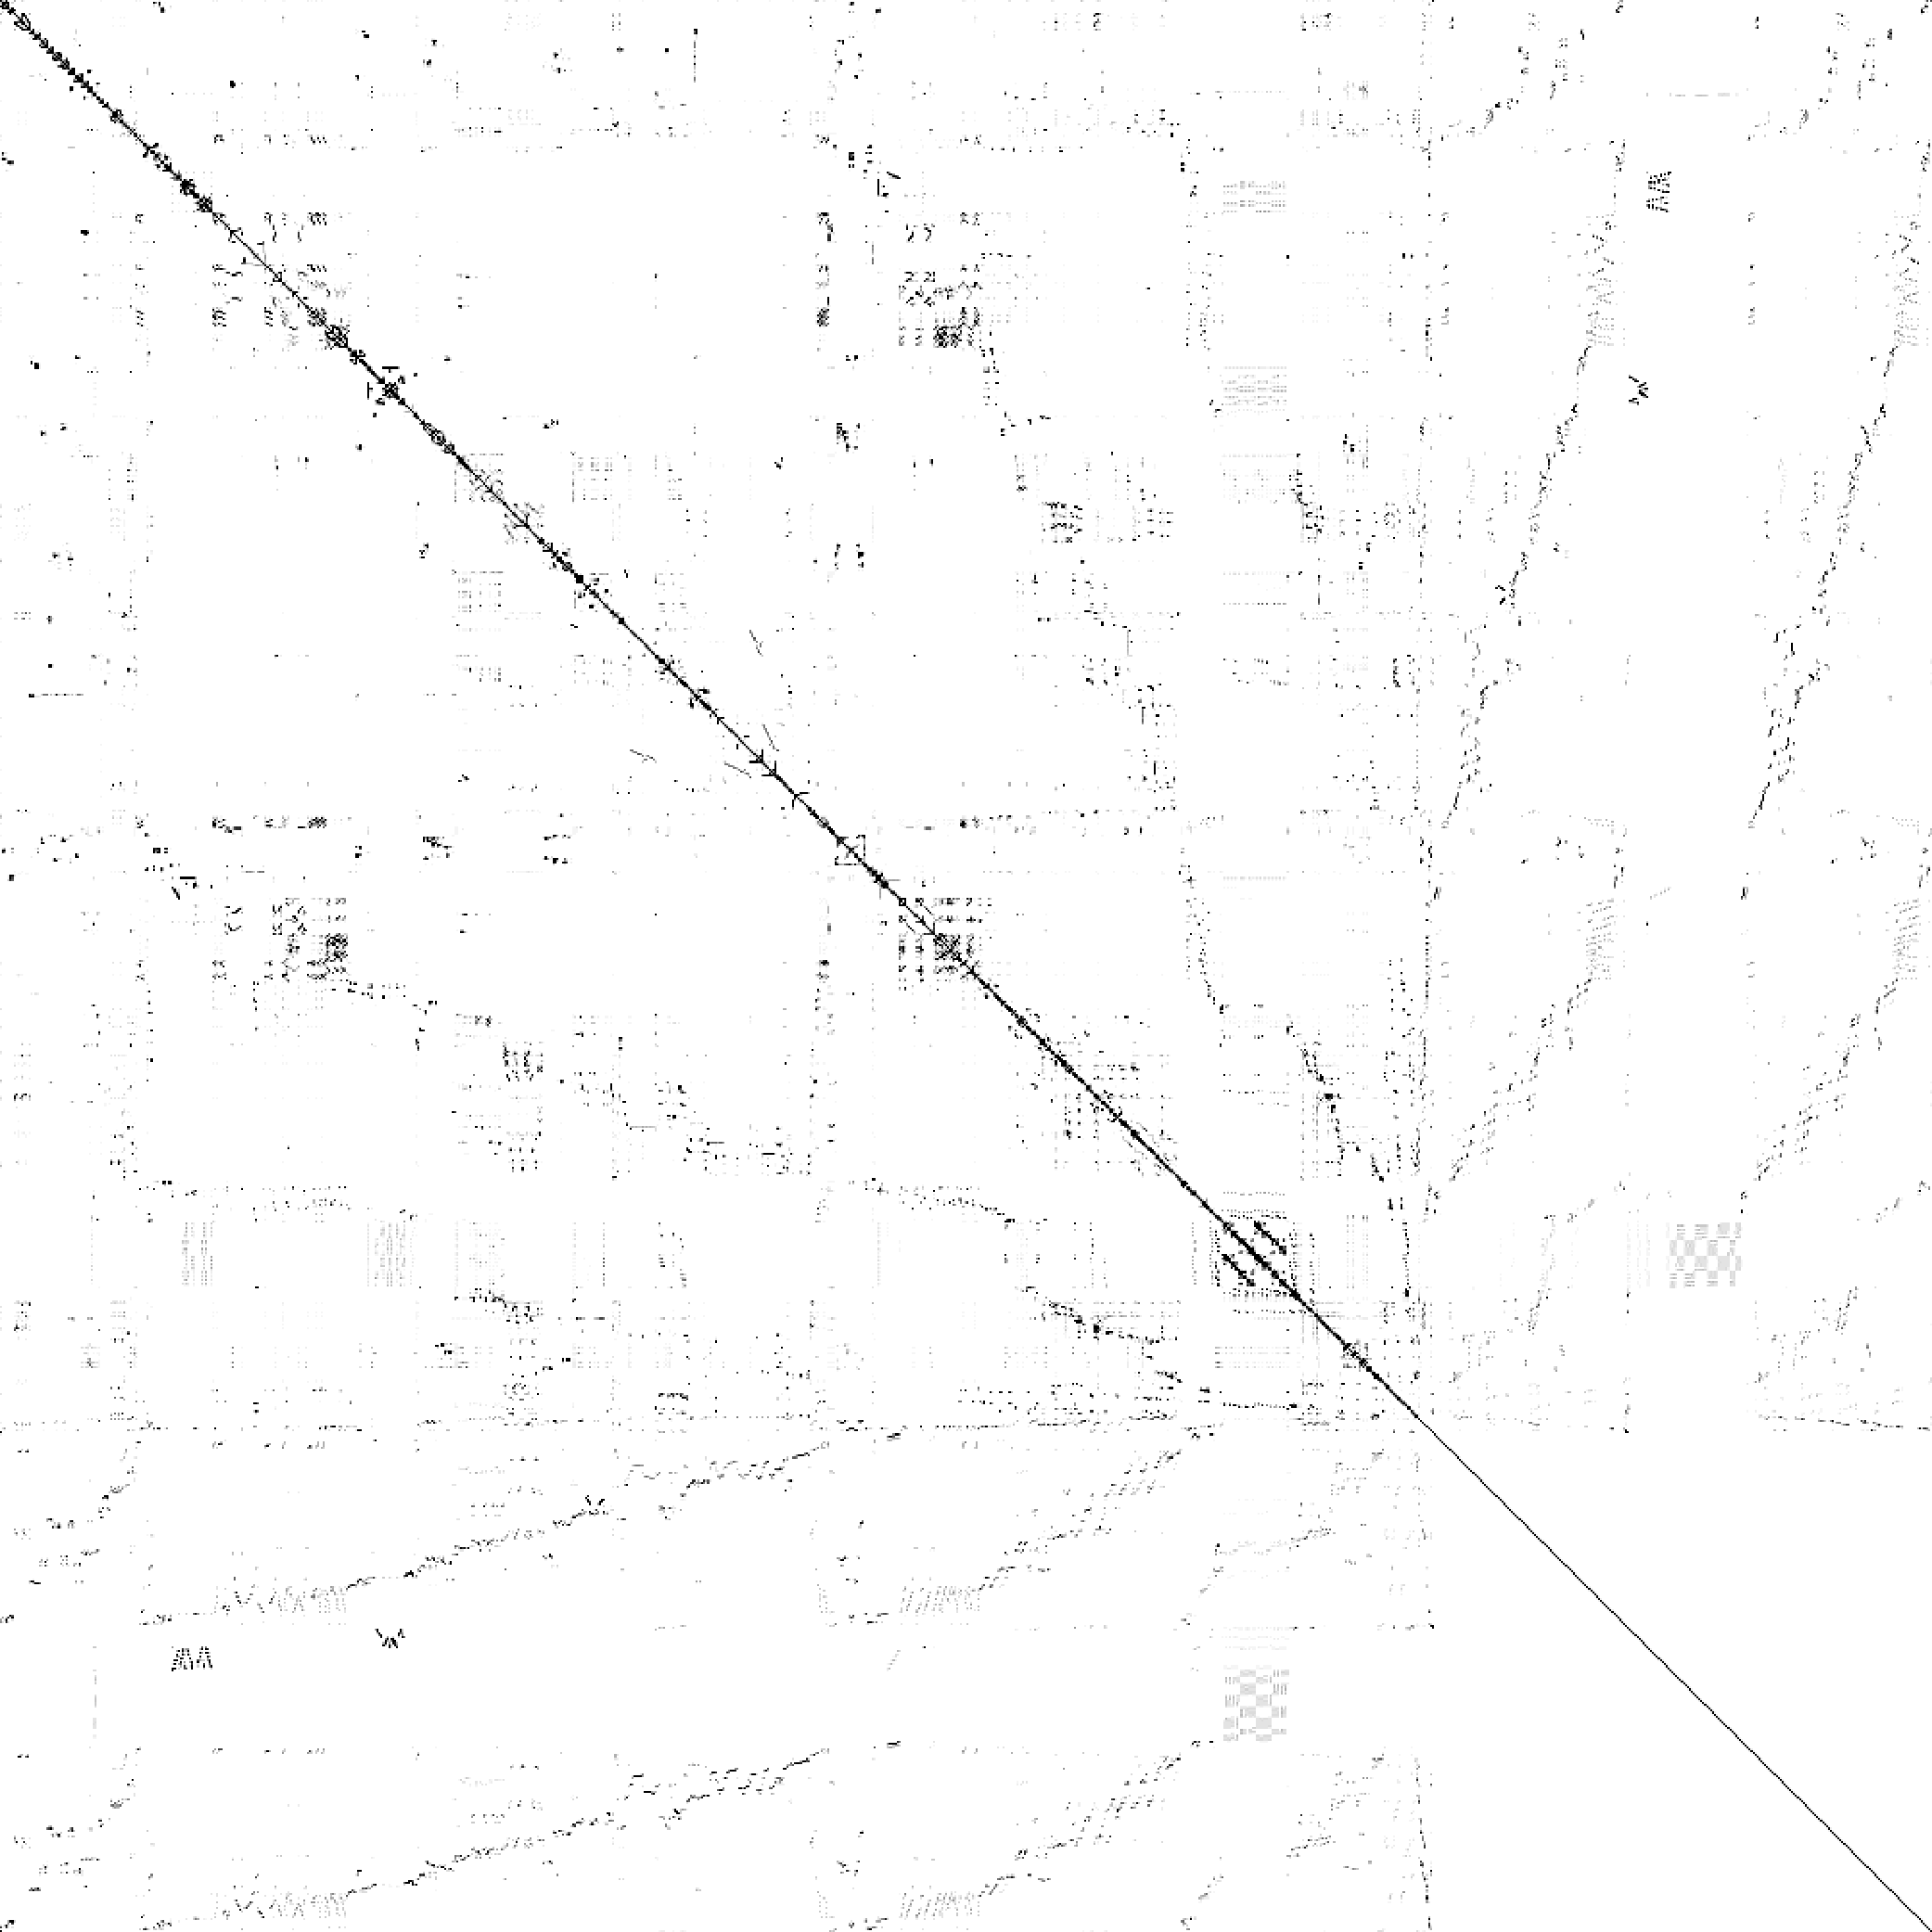
\includegraphics[width=\linewidth]{images/scircuit}
\caption{scircuit}
\end{subfigure}~%
\begin{subfigure}{\linewidth}
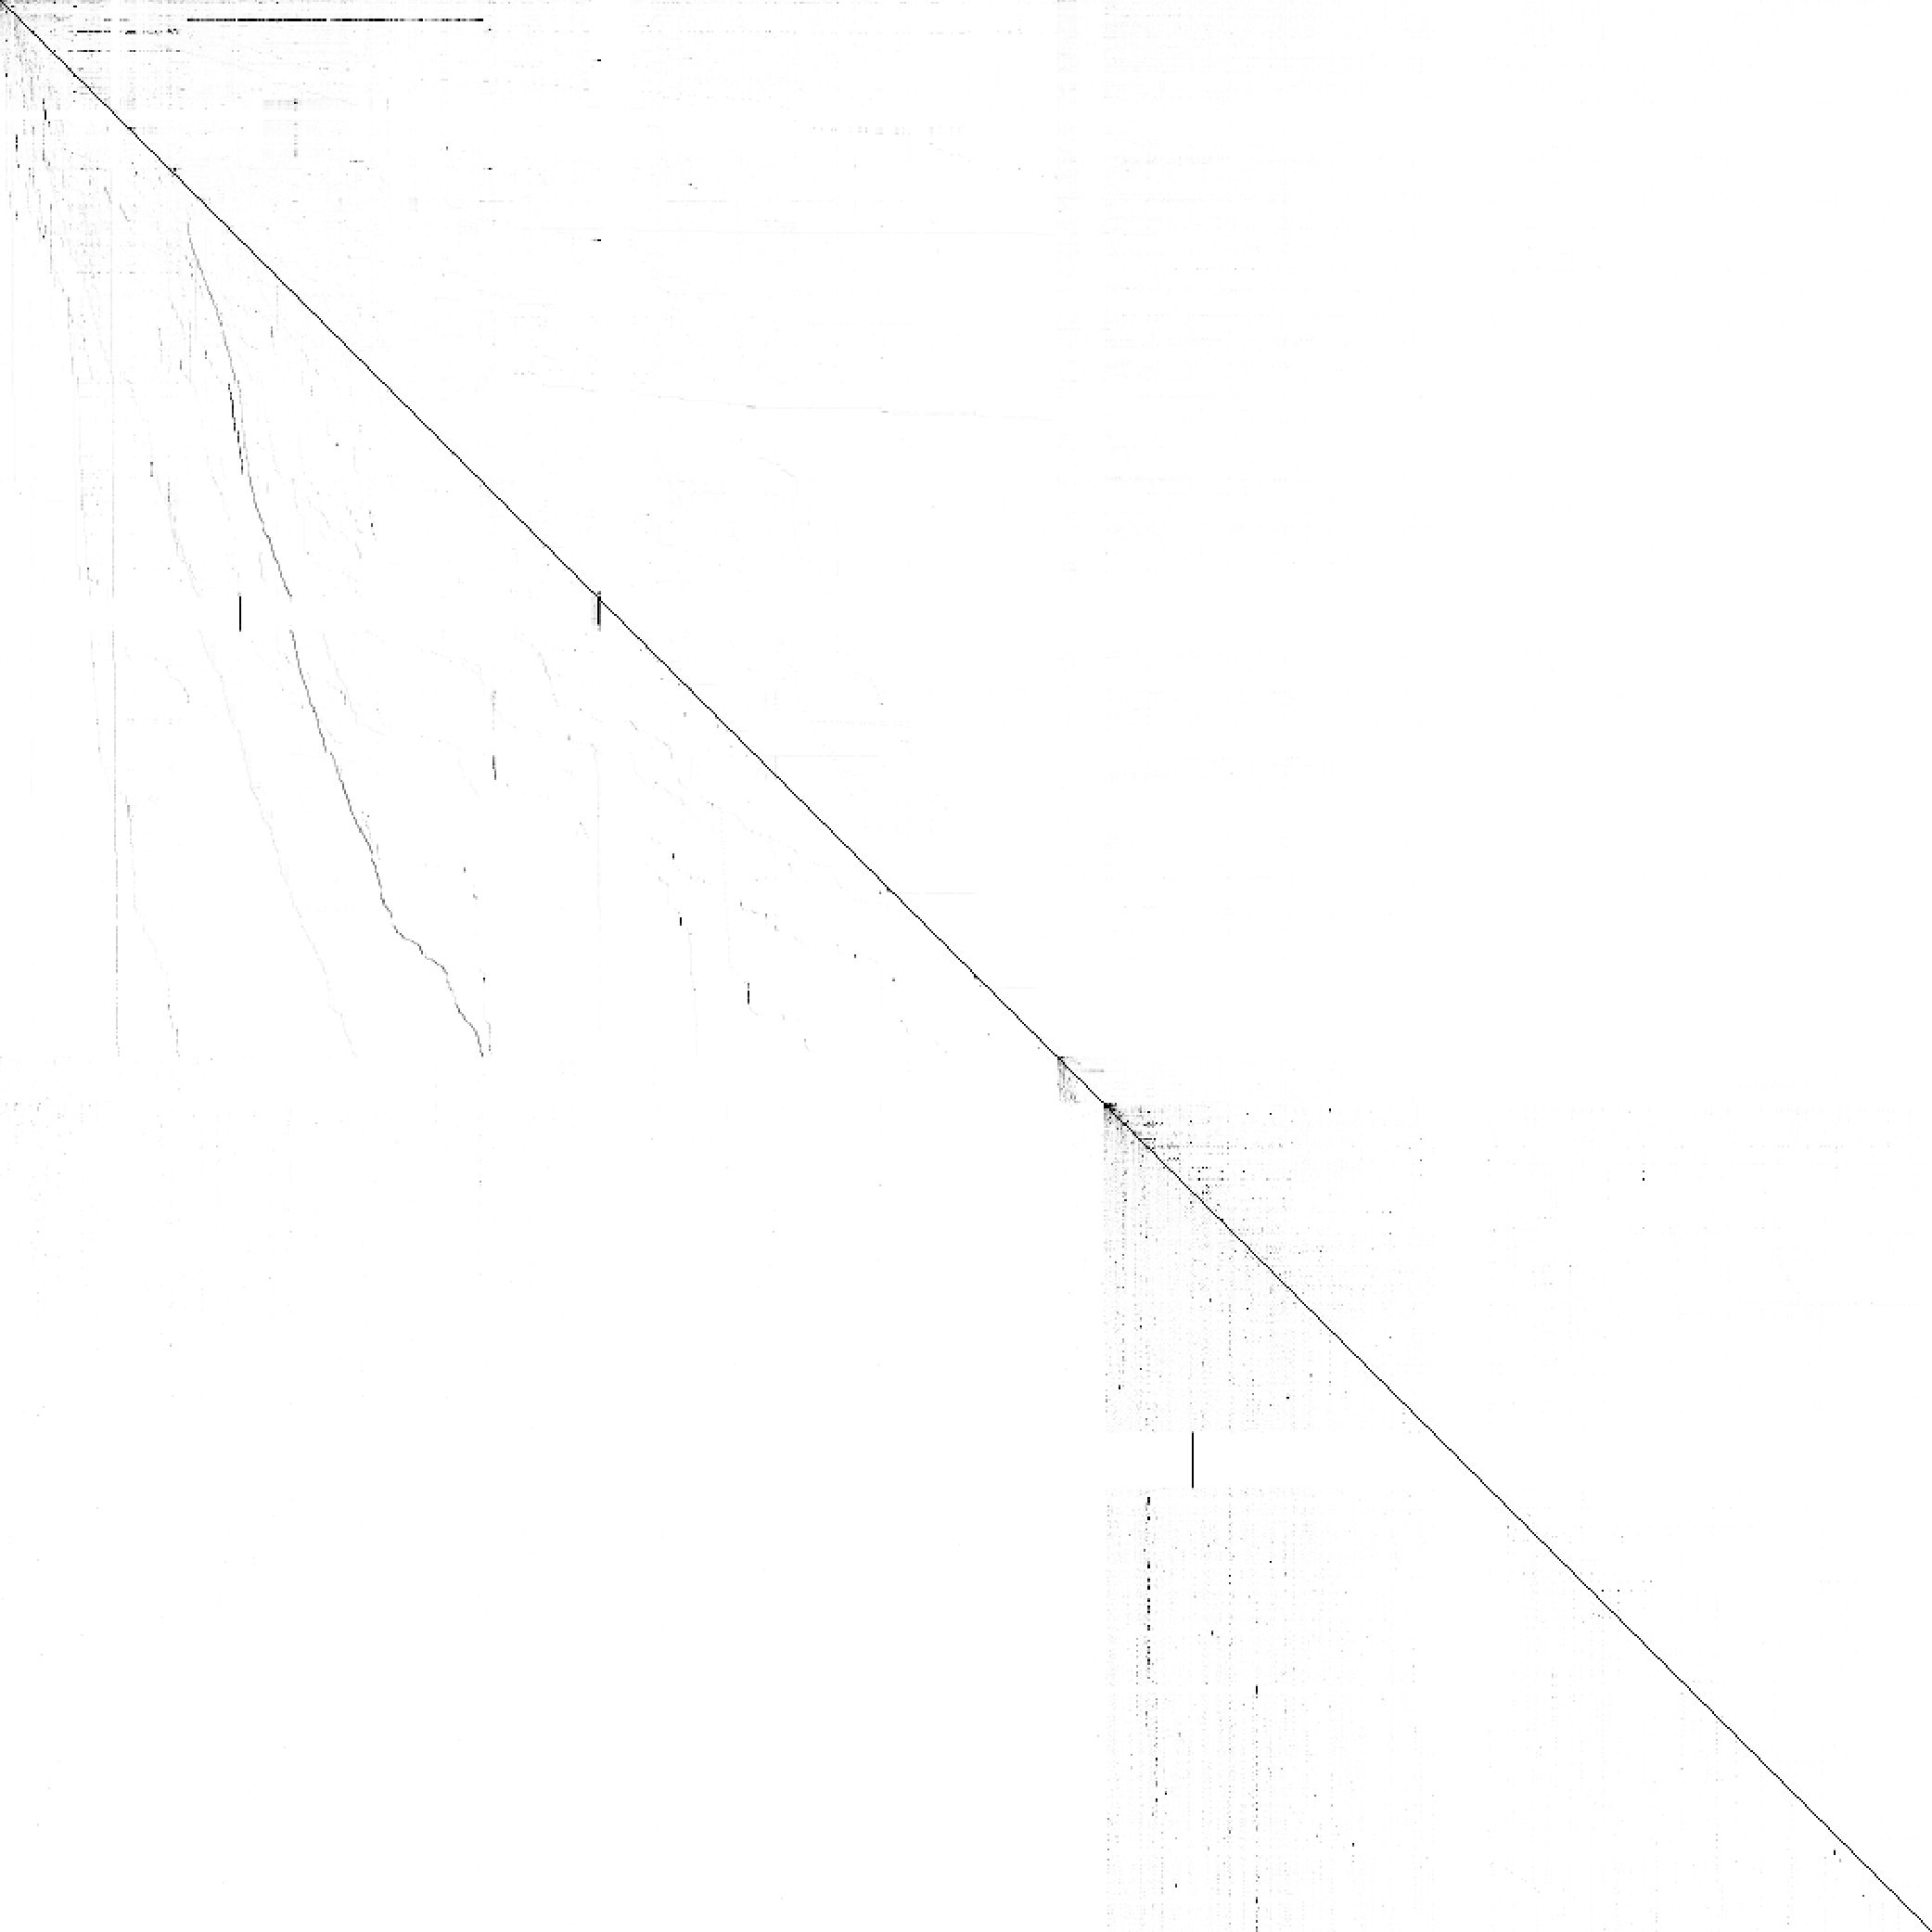
\includegraphics[width=\linewidth]{images/webbase-1M}
\caption{webbase-1M}
\end{subfigure}~%
\end{multicols}
\caption{The density plots of the matrices used for testing}
\end{figure}
\begin{figure}
\centering
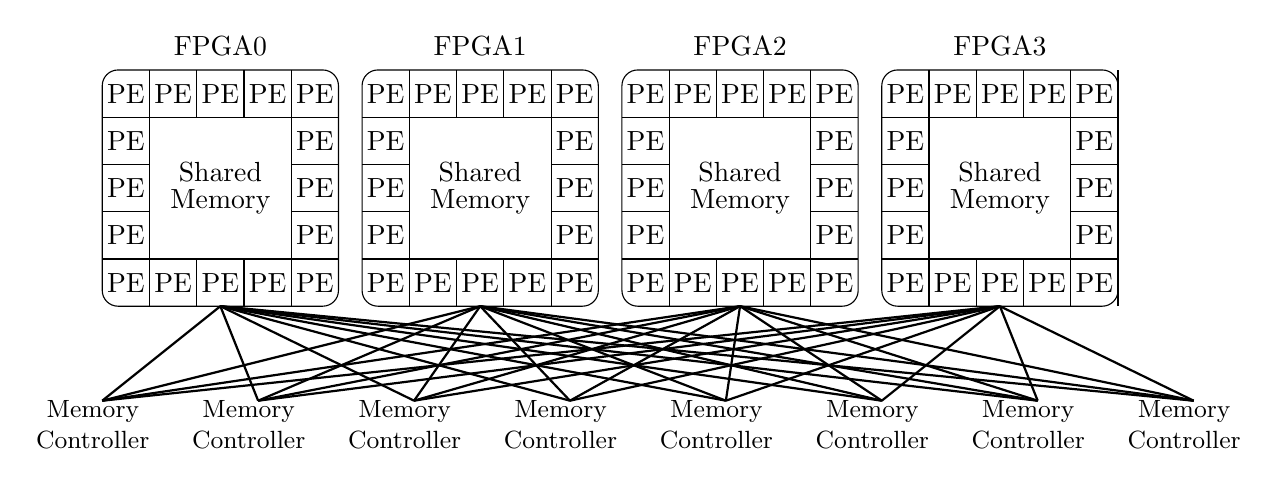
\begin{tikzpicture}[scale=.6]
\node at (3,6){FPGA0};
\node at (8.5,6){FPGA1};
\node at (14,6){FPGA2};
\node at (19.5,6){FPGA3};
\foreach \x in {1,...,4,5,6.5,7.5,...,10.5,12,13,...,16,17.5,18.5,...,21.5}
    \foreach \y in {1,...,5}
    {
        %\draw (\x, \y) +(-.5,-.5) rectangle ++(.5,.5);
        %\draw (\x, \y) node{\shortstack{$R^3$\\PE}};
        \draw (\x, \y) node{\shortstack{PE}};
    }
\foreach \x in {1.5,2.5,3.5,4.5,7,8,9,10,12.5,13.5,14.5,15.5,18,19,20,21,22}
{
    \path[draw] (\x, .5) -- (\x, 5.5);
}
\foreach \x in {.5,6,11.5,17}
{
    \foreach \y in {1.5,2.5,3.5,4.5}
    \path[draw] (\x, \y) -- (\x+5, \y);
}
\draw (.5,.5) [rounded corners=.2cm]rectangle (5.5,5.5);
\draw (6,.5) [rounded corners=.2cm]rectangle (11,5.5);
\draw (11.5,.5) [rounded corners=.2cm]rectangle (16.5,5.5);
\draw (17,.5) [rounded corners=.2cm]rectangle (22,5.5);
\foreach \x in {3,8.5,14,19.5}{
    \node at (\x, 3)[draw, fill=white, minimum width=1.8cm, minimum height=1.8cm,inner sep=0,outer sep=0]{\shortstack{Shared\\Memory}};
}
\foreach [count=\i] \x in {0,3.3,6.6,...,24}
{
    \FPeval{\minus}{round(\i-1,0)};
    %\draw (\x, -2) +(-.6,-.5) [rounded corners=.2cm] rectangle ++(1.2, .5);
    \small
    \draw (\x, -2) +(.3, 0) node[rectangle,rounded corners=.2cm]{\shortstack{Memory \\Controller\minus}};
    \normalsize
    %\draw (\x, -2) +(.3, 0) node{\shortstack{MC\i}};
}
\foreach \ae in {3, 8.5, 14, 19.5}
{
    \foreach \mc in {.5,3.8,7.1,...,25}
    {
        \draw[thick] (\ae, .5) -- (\mc, -1.5);
    }
}
%\path[draw, dashed] (.5,-.5) -- (18,-.5);
%\node at (9.25,-.5) [rectangle,fill=white,inner sep=2pt](a){40GB/s Sustained Memory Bandwidth};

\end{tikzpicture}
\caption{$R^3$ implementation on the Convey HC-2 coprocessor: 4 Virtex-5 LX330 FPGAs tiled with 16 $R^3$ SpMV processing elements (PE) each. Each Virtex-5 chip connects to all 8 memory controllers, which enables each chip to have access to all of the coprocessor's memory.}
\label{fig:highlevel}
\end{figure}

\section{Benchmarking}
Ok, now we have a good background about SpMV, the platform it can run on and optimizations for SpMV we need a way to determine who is the best. This when benchmarking comes in. However, different matrices can have vastly different performance. In figure~\ref{nnzVgflops} we show the performance of SpMV on CPUs, GPUs and FPGAs. As you can see the performance is very jumpy from matrix to matrix. 3 factors effect the performance: dimension, sparsity, and values. \par
The dimension of a matrix are the height ($M$), the width ($N$) and the number of nonzeros ($nnz$). These metrics effect different processors differently. \par
For CPUs the $nnz$ and $N$ are important values. As figure~\ref{nnzVgflops} shows when the matrix no longer fits in cache it takes a performance hit. It takes a second performance hit (not shown) when the width of the matrix and the therefor the length of the $x$ vector grows to the point when the $x$ vector also can not fit in cache. \par
For GPUs cache plays less of a role. However, two factors conspire against GPUs. The matrix formats they use and the amount of RAM on GPU boards. The best performing matrix formats of GPUs, ELLPACK and Block-ELLPACK, also introduce 0 values and take up the most memory space. GPU boards currently have at most 12GB of on board RAM compared to the 128 or more possible on CPUs. This means as matrices approach and go beyond 1 billion values then GPUs have to use worse performing matrix formats or be completely unable to perform SpMV. \par
TODO: FPGAs
TODO: sparsity
TODO: values
\begin{figure}
\centering
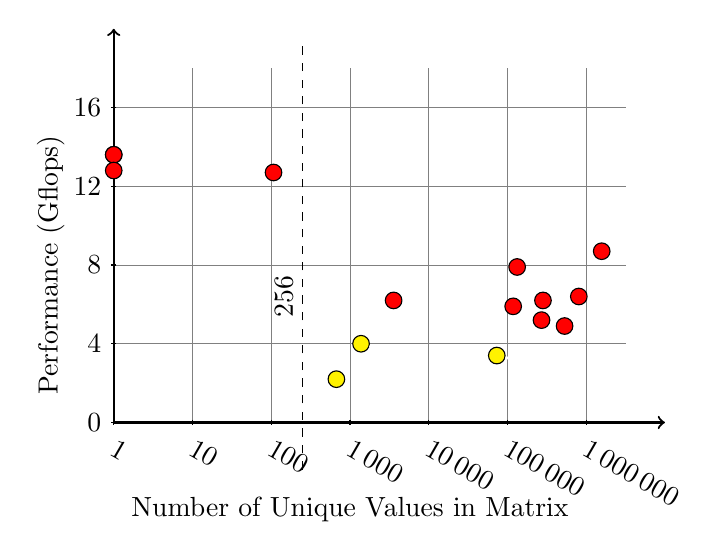
\begin{tikzpicture}
\draw[step=1.0,gray,very thin] (0,0) grid (6.5,4.5);
\draw [->,thick] (0,0) to (0,5);
\draw [->,thick] (0,0) to (7,0);
\foreach \x/\xtext in {0/1,1/10,2/100,3/1\,000,4/10\,000,5/100\,000,6/1\,000\,000}
	\draw (\x cm, 1pt) -- (\x cm, -1pt) node[anchor=north west,rotate=-30] {$\xtext$};
\foreach \y/\ytext in {0/0,1/4,2/8,3/12,4/16}
	\draw (1pt, \y cm) -- (-1pt,\y cm) node[anchor=east] {$\ytext$};

\foreach \i/\x/\y/\m/\s/\t/\a in {
0/0.0/3.4/dense/1/13.6/.3,%
1/0.0/3.4/rma10/1/13.6/-.1,%
2/0.0/3.2/qcd5\_4/1/12.8/-.4,%
3/2.0293837776852097/3.175/cant/107/12.7/0,%
6/3.5543680009900878/1.55/mc2depi/3584/6.2/.4,%
8/5.0730067708393705/1.475/mac\_econ\_fwd500/118306/5.9/.3,%
9/5.123400785682125/1.975/shipsec1/132862/7.9/.5,%
10/5.433/1.3/raefsky1/271382/5.2/.1,%
11/5.451272036830906/1.55/scircuit/282665/6.2/.3,%
12/5.725640521811938/1.225/psmigr\_2/531668/4.9/-.4,%
13/5.906686753316721/1.6/torso2/806653/6.4/-.1,%
14/6.197264013258786/2.175/consph/1574940/8.7/.3
%1/0/3.4/dense/1/13.6/.3, 1/0/3.4/rma10/1/13.6/-.1, 2/0/3.2/qcd5\_4/1/12.8/-.4, 3/2.03/3.175/cant/107/12.7/0, %
%6/3.5543680009900878/1.55/mc2depi/3584/6.2/.4,%
%8/5.0730067708393705/1.475/mac\_econ\_fwd500/118306/5.9/.3,%
%9/5.123400785682125/1.975/shipsec1/132862/7.9/.5,%
%10/5.451272036830906/1.55/scircuit/282665/6.2/.3,%
%11/5.725640521811938/1.225/psmigr\_2/531668/4.9/-.3,%
%12/5.906686753316721/1.6/torso2/806653/6.4/0,%
%13/6.197264013258786/2.175/consph/1574940/8.7/.3%
}
	\draw (\x,\y) [fill=red]circle (3pt) node[anchor=north west,rotate=60,xshift=4pt, yshift=\a cm, fill=white, inner sep=-2pt]{};

%outliers
\foreach \i/\x/\y/\m/\s/\t/\a in {%
4/2.828015064223977/0.55/dw8192/673/2.2/.6,%
5/3.1408221801093106/1.0/t2d\_q9/1383/4.0/-.1,%
7/4.864689034136851/0.85/epb1/73230/3.4/-.1%
}
	\draw (\x,\y) [fill=yellow]circle (3pt) node[anchor=north west,rotate=60,xshift=.4, yshift=\a cm, fill=white, inner sep=-2pt]{};


\draw [dashed] (2.4,-.6) -- (2.4,4.8) node [midway,above, sloped, xshift=-.5cm]{$256$};
\node at (3,-1.1) {Number of Unique Values in Matrix};
\node at (-.8,2) [rotate=90] {Performance (Gflops)};
\end{tikzpicture}
\caption[dont care]{Unique values in a matrix vs the performance of $R^3$. Matrices with fewer than 256 unique values (only common elements exist) enables $R^3$ format to compress much better. The \tikz \draw[fill=yellow] circle(3pt);'s are outliers due to their size (see Figure \ref{nnzVgflops}).}
\label{uniqueVgflops}
\end{figure}%

\begin{table*}
\caption{Matrix Statistics}
\label{matrix_stat}
\centering
\begin{tabular}{ccccccccc}
\hline
\bfseries Matrix & \bfseries Field & \bfseries dimensions & \bfseries nnz & \bfseries nnz/row \\
\hline
 dense & Example & 2,000x2,000 & 4,000,000 & 2,000 \\
consph & FEM/Speres & 83,334x83,334 & 6,010,480 & 72 \\
cant & FEM/Cantilever & 62,451x62,451 & 4,007,383 & 64 \\
rma10 & FEM/Harbor & 46,835x46,835 & 2,329,092 & 49 \\
qcd5\_4 & QCD & 49,152x49,152 & 1,916,928 & 39 \\
shipsec1 & FEM/ship & 140,874x140,874 & 3,568,176 & 25\\
mac\_econ\_fwd500 & Economics & 206,500x206,500 & 1,273,389 & 6.2 \\
mc2depi & Epidemiology & 525,825x525,825 & 2,100,225 & 4.0 \\
scircuit & Circuit & 170,998x170,998 & 958,936 & 5.6 \\
\hline
%webbase-1M & Webbase & 1,000,005x1,000,005 & 3,105,526 & 3.1 & 565 \\
%\hline
\end{tabular}
\end{table*}
\begin{table*}
\caption{Matrix Statistics}
\label{matrix_stat}
\centering
\begin{tabular}{ccccccccc}
\hline
\bfseries Matrix & \bfseries $\bf R^3$ Gflops & \multirow{1}{*}{\bfseries \shortstack{$\bf 2\times$ Intel E5-2690}} & \multirow{1}{*}{\bfseries \shortstack{Nvidia Tesla M2090}}\\
\hline
 dense &  13.6 & 14 & \bf 23\\
consph &  8.7 & 11 & \bf 15\\
cant &  12.7 & 12 & \bf 17\\
rma10 & 13.6 & \bf 24 & 11\\
qcd5\_4 &  12.8 & \bf 30 & 20\\
shipsec1 & 7.9 & 10 &\bf 11\\
mac\_econ\_fwd500 &  5.9 & \bf 23 & 6\\
mc2depi &  6.2 & 21 & \bf 22\\
scircuit &  6.2 & \bf 12 & 6\\
\hline
%webbase-1M & Webbase & 1,000,005x1,000,005 & 3,105,526 & 3.1 & 565 \\
%\hline
\end{tabular}
\end{table*}
\begin{figure*}
\centering
\begin{tikzpicture}[scale=1]

 \ifthenelse{\equal{\blackandwhite}{true}}{
	\tikzstyle{yellowStar}=[draw, diamond, fill=black!65, inner sep =1.5pt];
	\tikzstyle{blueGreenDiamond}=[draw, diamond, fill=black!75, inner sep =1.5pt];
	\tikzstyle{greenSquare}=[draw, rectangle, fill=black!50, inner sep =2.5pt];
	\tikzstyle{blueTriangle}=[draw, regular polygon, regular polygon sides=3, fill=black!35, inner sep =1.5pt];
 }{
	\tikzstyle{yellowStar}=[draw, star, star points=5, fill=yellow, inner sep =1.5pt];
	\tikzstyle{blueGreenDiamond}=[draw, diamond, fill=green!60!blue, inner sep =1.5pt];
	\tikzstyle{greenSquare}=[draw, rectangle, fill=green, inner sep =2.5pt];
	\tikzstyle{blueTriangle}=[draw, regular polygon, regular polygon sides=3, fill=blue, inner sep =1.5pt];
 }

%\draw [ystep=2.0,gray,very thin, xstep = 14] (0,0) grid (12.9, 6.9);
\draw [->,thick] (0,0) to (14.5, 0);
\draw [->, thick] (0,0) to (0,7);
\foreach \x/\mat/\size in { %
0/dw8192/42K, 1/t2d\_q9/87K, 2/epb1/95K, 3/raefsky1/290K, 4/psmigr\_2/540K, 6/torso2/1M%
}
	\draw (\x cm, 1pt) -- (\x cm, -1pt) node[anchor=east,rotate=90,gray] {\shortstack{\mat (\size)}};
\foreach \x/\mat/\size in { %
5/scircuit/960K, 7/mac\_econ/1.3M, 8/qcd5\_4/1.9M, 9/mc2depi/2.1M, 10/rma10/2.3M, 11/shipsec1/3.6M, 12/dense/4M, 13/cant/4M, 14/consph/6M%
}
	\draw (\x cm, 1pt) -- (\x cm, -1pt) node[anchor=east,rotate=90] {\shortstack{\mat (\size)}};
\foreach \y/\ytext in {0/0,1/5,2/10, 3/15, 4/20, 5/25, 6/30}
	\draw (1pt, \y cm) -- (-1pt, \y cm) node[anchor=east] {$\ytext$};
%\node at (6, -.8) {Size of Matrix (Millions)};
\node at (-1, 3) [rotate=90]{Performance (Gflops)};

%R3 line
\foreach \i/\j/\k/\l in {%
0/0.42000000000000004/1/0.76,  1/0.76/2/0.6599999999999999,  2/0.6599999999999999/3/1.04,  3/1.04/4/0.9800000000000001,  4/0.9800000000000001/5/1.24,  5/1.24/6/1.28,  6/1.28/7/1.1800000000000002,  7/1.1800000000000002/8/2.56,  8/2.56/9/1.24,  9/1.24/10/2.7199999999999998,  10/2.7199999999999998/11/1.58,  11/1.58/12/2.7199999999999998,  12/2.7199999999999998/13/2.54,  13/2.54/14/1.7399999999999998
}{
 \ifthenelse{\equal{\blackandwhite}{true}}{
	\draw [black] (\i,\j) -- (\k,\l);
 }{
	\draw [red] (\i,\j) -- (\k,\l);
 }
}

%hc1 line
\foreach \i/\j/\k/\l in {%
0/0.33999999999999997/1/0.5,  1/0.5/2/0.52,  2/0.52/3/0.78,  3/0.78/4/0.78,  4/0.78/6/0.24
}{
 \ifthenelse{\equal{\blackandwhite}{true}}{
	\draw [black!65] (\i,\j) -- (\k,\l);
 }{
	\draw [brown] (\i,\j) -- (\k,\l);
 }
}

%%tesla line
%\foreach \i/\j/\k/\l in {%
%0/0.1/1/0.18,  1/0.18/2/0.16,  2/0.16/3/0.5599999999999999,  3/0.5599/5/0.6}
%	\draw <3,5>[green!60!blue] (\i,\j) -- (\k,\l);

%m2090 line
\foreach \i/\j/\k/\l in {%
5/1.2/7/1.2,  7/1.2/8/4.0,  8/4.0/9/4.4,  9/4.4/10/2.2,  10/2.2/11/2.2,  11/2.2/12/4.6,  12/4.6/13/3.4,  13/3.4/14/3.0
}{
 \ifthenelse{\equal{\blackandwhite}{true}}{
	\draw [black!50] (\i,\j) -- (\k,\l);
 }{
	\draw [green] (\i,\j) -- (\k,\l);
 }
}

%intel line
\foreach \i/\j/\k/\l in {%
5/2.4/7/4.6,  7/4.6/8/6.0,  8/6.0/9/4.2,  9/4.2/10/4.8,  10/4.8/11/2.0,  11/2.0/12/2.8,  12/2.8/13/2.4,  13/2.4/14/2.2
}{
 \ifthenelse{\equal{\blackandwhite}{true}}{
	\draw [black!35] (\i,\j) -- (\k,\l);
 }{
	\draw [blue] (\i,\j) -- (\k,\l);
 }
}


\draw [dashed] (.5, -.5) -- (.5, 7) node [fill=white,inner sep=0pt, midway,below, sloped]{\small $(64K)$};

\draw [dashed] (10.5, -.5) -- (10.5, 7)  node [fill=white,inner sep=0pt, near end,below, sloped]{\small 20MB $(2.5M)$};



%hc1 points
\foreach \i/\x/\y/\f/\q/\u in {%
0/0.083492/0.33999999999999997/1.7/0/-.2,%
1/0.17405/0.5/2.5/0/-.1,%
2/0.190106/0.52/2.6/0/-.2,%
3/0.588552/0.78/3.9/0/-.2,%
4/1.080044/0.78/3.9/0/-.2,%
6/2.066946/0.24/1.2/0/0
}{
 \ifthenelse{\equal{\blackandwhite}{true}}{
	\draw (\i,\y) node[yellowStar]{} node[fill=white,inner sep=0pt, anchor=west,rotate=30,xshift=\q cm + 3pt, yshift=\u cm] {\color{black!65} \scriptsize $\f$};
 }{
	\draw (\i,\y) node[yellowStar]{} node[fill=white,inner sep=0pt, anchor=west,rotate=30,xshift=\q cm + 3pt, yshift=\u cm] {\color{brown} \scriptsize $\f$};
 }
}	

%intel points
\foreach \i/\x/\y/\f/\q/\u in {%
5/1.917872/2.4/12/0/0,%
7/2.546778/4.6/23/0/0,%
8/3.833856/6.0/30/0/0,%
9/4.20045/4.2/21/0/-.2,%
10/4.658184/4.8/24/0/0,%
11/7.136352/2.0/10/0/0,%
12/8.0/2.8/14/0/.2,%
13/8.014766/2.4/12/0/-.2,%
14/12.02096/2.2/11/0/0
}{
 \ifthenelse{\equal{\blackandwhite}{true}}{
	\draw (\i cm,\y cm) node[blueTriangle]{} node[fill=white,inner sep=0pt, anchor=west,rotate=30,xshift=\q cm + 3pt, yshift=\u cm]{\color{black!50} \scriptsize $\f$};
 }{
	\draw (\i cm,\y cm) node[blueTriangle]{} node[fill=white,inner sep=0pt, anchor=west,rotate=30,xshift=\q cm + 3pt, yshift=\u cm]{\color{blue} \scriptsize $\f$};
 }
}

%M2090 points
\foreach \i/\x/\y/\f/\q/\u in {%
5/1.917872/1.2/6/0/-.3,%
7/2.546778/1.2/6/0/.3,%
8/3.833856/4.0/20/0/0,%
9/4.20045/4.4/22/0/0,%
10/4.658184/2.2/11/0/0,%
11/7.136352/2.2/11/0/.1,%
12/8.0/4.6/23/0/0,%
13/8.014766/3.4/17/0/0,%
14/12.02096/3.0/15/0/0
}{
 \ifthenelse{\equal{\blackandwhite}{true}}{
	\draw (\i,\y) node[greenSquare]{} node[fill=white,inner sep=0pt, anchor=west,rotate=30,xshift=\q cm + 3pt, yshift=\u cm]{\color{black!35} \scriptsize $\f$};
 }{
	\draw (\i,\y) node[greenSquare]{} node[fill=white,inner sep=0pt, anchor=west,rotate=30,xshift=\q cm + 3pt, yshift=\u cm]{\color{green!100} \scriptsize $\f$};
 }
}

%R3 points
\foreach \i/\x/\y/\f/\q/\u in {%
0/0.083492/0.42000000000000004/2.1/0/0,%
1/0.17405/0.76/3.8/0/0,%
2/0.190106/0.6599999999999999/3.3/0/0,%
3/0.588552/1.04/5.2/0/0,%
4/1.080044/0.9800000000000001/4.9/0/0,%
5/1.917872/1.24/6.2/0/0,%
6/2.066946/1.28/6.4/0/0,%
7/2.546778/1.1800000000000002/5.9/0/0,%
8/3.833856/2.56/12.8/0/0,%
9/4.20045/1.24/6.2/0/0,%
10/4.658184/2.7199999999999998/13.6/0/0,%
11/7.136352/1.58/7.9/0/0,%
12/8.0/2.7199999999999998/13.6/0/0,%
13/8.014766/2.54/12.7/0/0,%
14/12.02096/1.7399999999999998/8.7/0/0
}{
 \ifthenelse{\equal{\blackandwhite}{true}}{
	\draw (\i,\y) [fill=black]circle(3pt) node(r\i)[fill=white,inner sep=0pt, anchor=west,rotate=30,xshift=\q cm + 3pt, yshift=\u cm]{\color{black} \scriptsize $\f$}; 
 }{
	\draw (\i,\y) [fill=red]circle(3pt) node(r\i)[fill=white,inner sep=0pt, anchor=west,rotate=30,xshift=\q cm + 3pt, yshift=\u cm]{\color{red} \scriptsize $\f$};
 }
}

\draw (4,5.5) node (key)[rectangle,minimum width=4cm, minimum height=2.7cm]{};
 \ifthenelse{\equal{\blackandwhite}{true}}{
	\node at (key) [rectangle,anchor=west, xshift=-2cm, yshift=1cm]{\tikz{\draw (0,1pt) [fill=black]circle (2.5pt);} $R^3$};
 }{
	\node at (key) [rectangle,anchor=west, xshift=-2cm, yshift=1cm]{\tikz{\draw (0,1pt) [fill=red]circle (2.5pt);} $R^3$};
 }
\node at (key) [rectangle,anchor=west, xshift=-2cm, yshift=.3cm]{\shortstack{\tikz{\draw (0,1pt) node[yellowStar]{};} \cite{prelim:nagar1} }};
%\node <3,5>at (key) [rectangle,anchor=west, xshift=-2cm, yshift=0cm]{\tikz{\draw (0,1pt) node[blueGreenDiamond]{};} Nvidia Tesla S1070};
\node at (key) [rectangle,anchor=west, xshift=-2cm, yshift=-.5cm]{\shortstack{\tikz{\draw (0,1pt) node[greenSquare]{};} Nvidia Tesla \\M2090}};
\node at (key) [rectangle,anchor=west, xshift=-2cm, yshift=-1.5cm]{\shortstack{\tikz{\draw (0,1pt) node[blueTriangle]{};} Intel E5-2690 \\(2 CPUs)}};

\end{tikzpicture}
\caption{$nnz$ vs Performance on each platform. The small matrices, ones around 64K or less, performed poorly on $R^3$, due to the overhead. CPUs experience the opposite effect. They take a performance hit once the matrix no longer fits in cache.}
\label{nnzVgflops}
\end{figure*}

%%\chapter{SpMV on FPGA METHODOLOGY}
\label{chp:method}

\begin{figure}
    \centering
    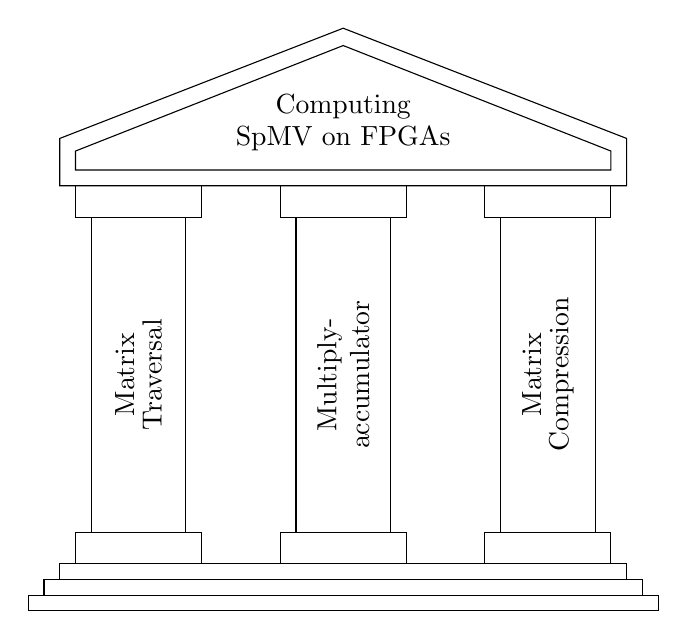
\begin{tikzpicture}[scale=2]
        \draw (0,0) rectangle (4,.1);
        \draw (.1,.1) rectangle (3.9,.2);
        \draw (.2,.2) rectangle (3.8,.3);

        \draw (.3,.3) rectangle (1.1,.5);
        \draw (1.6,.3) rectangle (2.4, .5);
        \draw (2.9, .3) rectangle (3.7, .5);
        \draw (.4,.5) rectangle (1,2.5);
        \node at (.7,1.5) [rotate=90]{\shortstack{Matrix\\Traversal}};

        \draw (1.7,.5) rectangle (2.3,2.5);
        \node at (2,1.5) [rotate=90]{\shortstack{Multiply-\\accumulator}};

        \draw (3,.5) rectangle (3.6,2.5);
        \node at (3.3,1.5) [rotate=90]{\shortstack{Matrix\\Compression}};

        \draw (.3,2.5) rectangle (1.1,2.7);
        \draw (1.6,2.5) rectangle (2.4, 2.7);
        \draw (2.9, 2.5) rectangle (3.7, 2.7);

        \draw (.2,2.7) -- (3.8,2.7) -- (3.8,3) -- (2,3.7) -- (.2,3) -- cycle;
        \draw (.3,2.8) -- (3.7,2.8) -- (3.7, 2.92) -- (2,3.59) -- (.3,2.92) -- cycle;
        \node at (2,3.1) {\shortstack{Computing\\SpMV on FPGAs}};
    \end{tikzpicture}
    \caption{Because different aspects limit the performance of SpMV on FPGAs, no one optimization will lead to significant benefit for SpMV. We identified these three optimizations that together lead to a significant performance benefit.}
    \label{fig:pillars}
\end{figure}

In the previous chapter, we have discussed how others have approached computing SpMV on FPGAs and other processors. We build upon some of the good ideas and add our own. When these pillars are in place the dataflow of the design still looks the same as other implementations (\figurename~\ref{fig:dataflow}). The architecture diagram also follows the same general flow of the dataflow diagram (\figurename~\ref{fig:SpMV}).
Three pillars emerged during the design of the hardware description and software: designing the traversal of the matrix, designing the multiply-accumulator, and designing the matrix compression (\figurename~\ref{fig:pillars}). The next three sections describe these pillars and the interactions between them.

\section{First Pillar: Matrix Traversal}
\par The first pillar, matrix traversal, primarily helps with vector reuse. Column traversal has a major effect on vector reuse. Many papers argue that vector caching is the way to achieve $x$ vector reuse for FPGAs [\cite{prelim:umuroglu, prelim:nagar1}] (TODO: more cites). We disagree. With the ability to use column traversal in a horizontal subsection of say 1000 rows one can perfectly reuse vector values in this section. This requires the storage of 1000 intermediate y values or 8KB. Compare this to caching. Assume there are 10 non-zero elements per row and assume each vector value gets accessed twice. Then to achieve good caching the cache must support 5000 values or 40KB. This also ignores storing the vector indices of the cached values. So, in this example, storing intermediate values is more than 5 times more space efficient than vector caching.
\par The second advantage of mixing row and column traversal is that it leads to smaller deltas. In this paper, a delta is the traversal distance between a matrix element and its preceding matrix element in the traversal. To achieve high $x$ vector reuse and small deltas we use row-column-row traversal. Chapter \ref{chp:traversal} discusses matrix traversal in detail.

\section{Second Pillar: Multiply-accumulator}

\par The second pillar, the multiply accumulator, has to accumulate multiple rows at a time to allow different traversals (the first pillar). Several multiply-accumulators exists, but they rely on row-major traversal \cite{}. Although, we do use pre-existing floating-point cores created by Flopoco [\cite{}]. We created an IP core called the Intermediator, which stores intermediate $y$ values and allows for row-column-row traversal. Chapter \ref{chp:mac} discusses the multiply-accumulator in detail.

\section{Third Pillar: Matrix Compression}
\par The third pillar, compression, may be the most important for FPGAs. Compression of the matrix has a large amount of importance, because reading the matrix takes up a majority of the memory bandwidth. The current view in the SpMV field does not count preprocessing of the matrix towards the SpMV runtime. This is because SpMV is usually used in iterative and repetitive methods. We agree with this sentiment.
\subsection{Index compression}
\par Using deltas to compress indices is the first and easiest step towards this pillar. Many compression implementations try to align variable length encoding to 4 bit or other size boundaries. We give little regard to boundaries because we find the added compression to be worth the extra FPGA space the decoder needs. Chapter \ref{chp:compression} discusses delta compression in detail.
%
\subsection{Floating Point Compression}
\par Value compression is tricky but has a potential to save large amounts of space and thus memory bandwidth. Values repeat more than one would expect in matrices \cite{}. Taking advantage of this repetition is the biggest step towards good compression. \figurename~\ref{fig:uniqueVgflops} shows how much of an effect this pattern has on the performance of our previous SpMV implementation, $R^3$. Chapter \ref{chp:fzip} discusses floating point compression in detail.

\subsection{Multi-port Shared Memory}
\par Because good value compression requires a significant amount of on-chip memory space, we designed a shared memory IP block. This means instead of using 1 RAM block on each PE to store the 512 most common floating point values, we use one RAM block per PE to create a large shared memory to store the 8,192 most common floating point values. Chapter \ref{chp:memory} discusses the design of the shared memory IP block.%
%
\begin{figure}
\centering
\begin{tikzpicture}[scale=1]
\draw [dashed](-6,0) -- (4,0);
\node at (.1,-2) {\large \shortstack{External\\Memory}};
\node at (.1,-1) [draw, trapezium, trapezium right angle=70, trapezium left angle=-70,  minimum width=1.5cm, minimum height=1cm, inner xsep=-7pt](x){$x$ Vector};
\node at (-3,-1.25) [draw,trapezium, trapezium right angle=70, trapezium left angle=-70,  minimum width=1.5cm, minimum height=1.5cm, inner xsep=-12pt](a){$A$ Matrix};
\node at (2.5,-1) [draw, trapezium, trapezium right angle=70, trapezium left angle=-70, minimum width=0cm, minimum height=1cm, inner xsep=-7pt](y){$y$ Vector};

\node at (0, 3) {\large $R^3$ Processing Element};
\draw [dashed] (-6,1.5) -- (-3,1.5);
\node at (-4.5, 1.5) [draw, rectangle, minimum height=2cm, minimum width=3cm](dec){};
\node at (-5.3,1.5)[rotate=90, anchor=south,fill=white]{Decoder};
\node at (-4.5,2) {Value};
\node at (-4.5,1) {Index};
\node at (-4.5, 3.5) [color=black](vCache){Shared Memory};
\path [draw, color=black] (vCache.north east) to (vCache.south east) to (vCache.south west) to (vCache.north west);
\node at (1,1.5) [draw, rectangle, minimum height=2.1cm, minimum width=5cm, label={[label distance=-.5cm]90:Multiply-Accumulator}](acc){};
\node at (acc) [draw, rectangle, xshift=1.8cm, yshift=-.2cm, minimum height=1cm](add){Adder};
\node at (acc) [draw, rectangle, xshift=0cm, yshift=-.2cm, minimum height=1cm](int){\shortstack{Inter-\\mediator}};
\node at (acc) [draw, rectangle, xshift=-1.8cm, yshift=-.2cm, minimum height=1cm](mult){\shortstack{Multi-\\plier}};

\path [draw, thick, >=stealth',->, shorten >=2pt](a) to [] node[fill=white, inner sep=1pt, pos=.4]{\shortstack{val+\\row+col}}(dec);
\path [draw, thick, >=stealth',->, shorten >=2pt, label={[above,sloped]{column}}](dec) to [] node[sloped, fill=white, inner sep=1pt]{col} (x);
\path [draw, thick, >=stealth',->, shorten >=2pt](dec.20) to node[sloped, fill=white, inner sep=1pt]{val} (mult);
\path [draw, thick, >=stealth',->, shorten >=2pt](dec.-20) to node[sloped, fill=white, inner sep=1pt]{row} (mult);
\path [draw, thick, >=stealth',->, shorten >=2pt](mult.120) to [bend left = 30] node[sloped, fill=white, inner sep=1pt]{val+row} (int);

\path [draw, thick, >=stealth',->, shorten >=2pt](x) to [] node[sloped, fill=white, inner sep=1pt]{val} (mult);
\path [draw, thick, >=stealth',->, shorten >=2pt](int.north) to [bend left = 20] node[sloped, fill=white, inner sep=1pt]{val+val+row} (add.50);
\path [draw, thick, >=stealth',->, shorten >=2pt](add.-50) to [bend left = 40] node[sloped, fill=white, inner sep=1pt]{val+row} (int);
\path [draw, thick, >=stealth', ->, shorten >= 2pt](int) .. controls (1,0) and (2.1,0) .. node[sloped, fill=white, inner sep=1pt]{val}  (y);
\path [draw, gray, thick, >=stealth', <->, shorten >=2pt] (vCache) -- (dec);

\end{tikzpicture}
\caption[Diagram of a single processing element]{A single processing element. The arrows show the flow of data through the processing element. Although this diagram shows the memory access to each of the 3 places in memory as separate, they share one memory port. The diagram also does not show the FIFOs that help keep the pipeline full.}
\label{fig:SpMV}
\end{figure}%
%

\begin{figure}
\centering
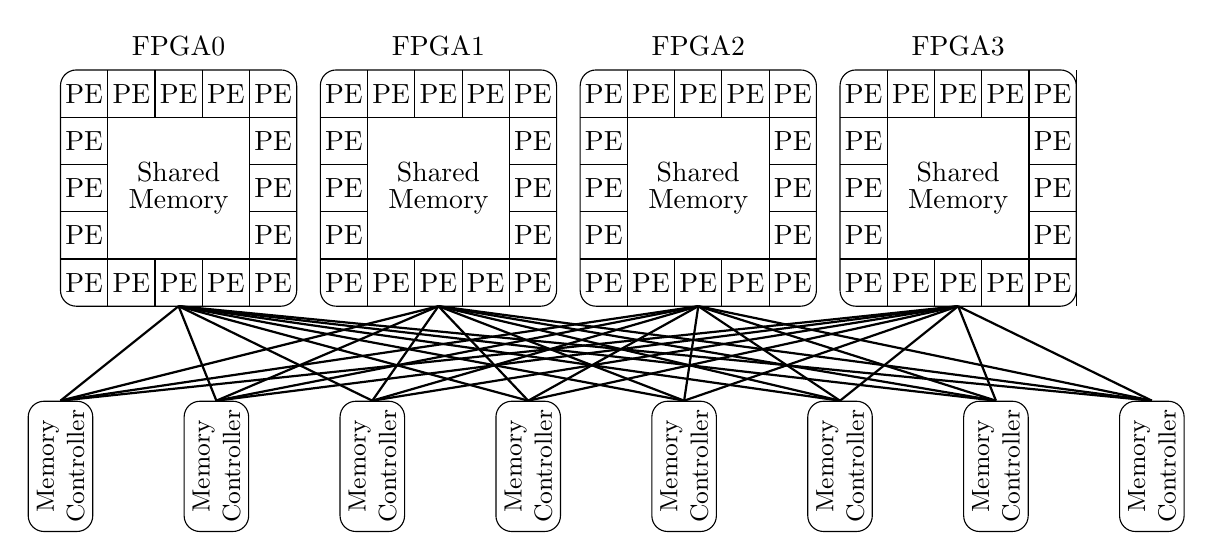
\begin{tikzpicture}[scale=.6]
\node at (3,6){FPGA0};
\node at (8.5,6){FPGA1};
\node at (14,6){FPGA2};
\node at (19.5,6){FPGA3};
\foreach \x in {1,...,4,5,6.5,7.5,...,10.5,12,13,...,16,17.5,18.5,...,21.5}
    \foreach \y in {1,...,5}
    {
        %\draw (\x, \y) +(-.5,-.5) rectangle ++(.5,.5);
        %\draw (\x, \y) node{\shortstack{$R^3$\\PE}};
        \draw (\x, \y) node{\shortstack{PE}};
    }
\foreach \x in {1.5,2.5,3.5,4.5,7,8,9,10,12.5,13.5,14.5,15.5,18,19,20,21,22}
{
    \path[draw] (\x, .5) -- (\x, 5.5);
}
\foreach \x in {.5,6,11.5,17}
{
    \foreach \y in {1.5,2.5,3.5,4.5}
    \path[draw] (\x, \y) -- (\x+5, \y);
}
\draw (.5,.5) [rounded corners=.2cm]rectangle (5.5,5.5);
\draw (6,.5) [rounded corners=.2cm]rectangle (11,5.5);
\draw (11.5,.5) [rounded corners=.2cm]rectangle (16.5,5.5);
\draw (17,.5) [rounded corners=.2cm]rectangle (22,5.5);
\foreach \x in {3,8.5,14,19.5}{
    \node at (\x, 3)[draw, fill=white, minimum width=1.8cm, minimum height=1.8cm,inner sep=0,outer sep=0]{\shortstack{Shared\\Memory}};
}
\foreach [count=\i] \x in {.5,3.8,7.1,...,25} %0,3.3,6.6,...,24}
{
    \FPeval{\minus}{round(\i-1,0)};
    %\draw (\x, -2) +(-.6,-.5) [rounded corners=.2cm] rectangle ++(1.2, .5);
    \small
    \draw (\x, -1.5) node[draw, rectangle,rounded corners=.2cm,rotate=90,anchor=east]{\shortstack{Memory \\Controller~\minus}};
    \normalsize
    %\draw (\x, -2) +(.3, 0) node{\shortstack{MC\i}};
}
\foreach \ae in {3, 8.5, 14, 19.5}
{
    \foreach \mc in {.5,3.8,7.1,...,25}
    {
        \draw[thick] (\ae, .5) -- (\mc, -1.5);
    }
}
%\path[draw, dashed] (.5,-.5) -- (18,-.5);
%\node at (9.25,-.5) [rectangle,fill=white,inner sep=2pt](a){40GB/s Sustained Memory Bandwidth};

\end{tikzpicture}
\caption[Modified high-level diagram of the Convey HC-2ex]{Our implementation has one shared memory for storing repeating values in the sparse matrices.}
\label{fig:highlevel2}
\end{figure}
\section{High Level Design}
Designing high performance reconfigurable computing implementations has a general two step process, which we follow. First, design one processing element (PE) to solve the problem (see \figurename~\ref{fig:SpMV}). Second, replicate that PE until all the FPGAs are full. In addition, we have a shared memory (see \figurename~\ref{fig:highlevel2}).

The PEs recieve instructions through a 1D systolic array. Each PE has 14 registers. Each PE has 8 instructions: RESET, READ\_REGISTER, WRITE\_REGISTER, WRITE\_DELTA\_CODES, WRITE\_FZIP\_CODES, WRITE\_SHARED\_MEMORY, and COMPUTE\_SPMV.

The PE themselves have 2 major components. First, the decoder block that requests the compressed matrix data and decodes it into row and column indices and floating point values. Second, the multiply-accumulator, where the actual SpMV computation takes place.

To Parallelize the SpMV computation we split the problem into $N$ smaller SpMV computations each given to one processing element. In hardware we connect each processing element to an external memory port and a shared memory port. Chapter \ref{chp:memory} discusses the high level design in detail.
%\par We separate our contributions into 5 pieces, the next 5 chapters. Chapter~\ref{chp:mac} focuses entirely on the first pillar, the multiply accumulator design. Chapter~\ref{chp:compression} focuses on pillars 2 and 3 with discussing matrix traversal and compressing indices with delta compression. Chapter~\ref{chp:fzip} focuses on the second part of pillar 3, value compression. We found good value compression requires a large amount of on-chip memory, therefore, Chapter~\ref{chp:memory} focuses on the design of a large memory shared by multiple processing elements.

%%\chapter{MULTIPLY-ACCUMULATOR}
\label{chapter:mac}
\begin{figure}
\hspace{-10pt}
\begin{tikzpicture}[scale=1]
\clip (-5,-2.5) rectangle (5,2.5);
\node at (0,0) [draw, rectangle, minimum height=4cm, minimum width=8cm, label={[label distance=-.6cm,xshift=-2cm]90:Multiply-Accumulator}](acc){};
\node at (acc) [draw, rectangle, xshift=3cm, yshift=0cm, minimum height=1cm, minimum width=2cm](add){Adder};
\node at (acc) [draw, rectangle, xshift=.3cm, yshift=0cm, minimum height=1cm, minimum width=0](int){\shortstack{Intermediator}};
\node at (acc) [draw, rectangle, xshift=-3cm, yshift=0cm, minimum height=1cm, minimum width=2cm](mult){\shortstack{Multiplier}};

\path [draw, thick, >=stealth',->] (-5,.3) --node[ fill=white, inner sep=1pt]{val} (-4,.3) ;
\path [draw, thick, >=stealth',->] (-5,0) --node[ fill=white, inner sep=1pt]{val} (-4,0) ;
\path [draw, thick, >=stealth',->] (-5,-.3) --node[ fill=white, inner sep=1pt]{row} (-4,-.3);

\path [draw, thick, >=stealth',->] (-2,0) --node[ fill=white, inner sep=1pt]{val} (-1,0);
\path [draw, thick, >=stealth',->] (-2,-.3) --node[ fill=white, inner sep=1pt]{row} (-1,-.3) ;

\path [draw, thick, >=stealth',->] (.4,.5)  arc(160:20:1.2);
\node at (1.5,1.2)[fill=white, inner sep=1pt]{row};

\path [draw, thick, >=stealth',->] (.1,.5)  arc(163:17:1.5);
\node at (1.5,1.5)[fill=white, inner sep=1pt]{val};

\path [draw, thick, >=stealth',->] (-.2,.5)  arc(166:14:1.8);
\node at (1.5,1.8)[fill=white, inner sep=1pt]{val};

\path [draw, thick, >=stealth',->] (2.6,-.5)  arc(-20:-160:1.2);
\node at (1.5,-1.2)[fill=white, inner sep=1pt]{row};

\path [draw, thick, >=stealth',->] (2.9,-.5)  arc(-17:-163:1.5);
\node at (1.5,-1.5)[fill=white, inner sep=1pt]{val};

\path [draw, thick, >=stealth',->] (-.5,-.5) --node[sloped, fill=white, inner sep=1pt]{val} (-.5,-2.5);
\end{tikzpicture} %

\caption{The no-stall multiply-accumulator block handles multiple intermediate values at a time. This allows multiple intermediate values in the adder pipeline.}
\label{mac}
\end{figure}
A high throughput SpMV implementation relies on designing a no-stall multiply accumulator (MAC). An inefficient engine stalls when a matrix and its associated vector value arrives every or nearly every clock cycle. The long latency of floating point addition makes this hard. To solve this, our approach works on multiple intermediate $y$ vector values and does the additions out of order. For example in computing $1+2+3+4$ the MAC does $(1+2)+(3+4)$. This removes the data dependency of adding $1$ and $2$ before processing $3$. CPUs and GPUs compute floating point addition in order (eg. $((1+2)+3)+4$). This means results may differ slightly, because changing the order of floating point addition can change the result [\cite{prelim:goldberg}].\\
\indent In $R^3$ [\cite{prelim:townsend}] we designed a block called an Intermediator (Section \ref{sec:intermediator}) capable of storing 32 intermediate $y$ vector values. In our next design we intend to expand this to 1024 (the depth of one dual port BlockRAM in most Xilinx chips). Both designs have an interesting side effect that the allow the matrix to be traversed in a loosely row major traversal and the MAC will still work correctly. The step to from 32 to 1024 intermediate values allows more freedom in the traversal. The rest of the chapter discusses the new design. The matrix elements in one set of 512 rows can be traversed in any way just as long as all the elements are traversed before going to the next 512 rows. Later in chapter 5 we discuss traversals that abide by this rule and allow for easy reuse of $x$ vector values. We plan to use a traversal that follows this rule called row column row (RCR) traversal.
\section{Intermediator}
\label{sec:intermediator}
The Intermediator (Figure \ref{intermediatorEx}) takes in two values, one from the multiplier's result and one from the adder's result and outputs a pair of values to be added. The dual-port Block RAM (middle block in Figure \ref{intermediatorEx}) stores intermediate values until an element in the same row appears. \par
For most matrices, the Block RAM cannot store the entire intermediate $y$ vector. Also the control logic needs to remember the state of each slot in RAM (empty or full). Remembering the state of each RAM location and updating that state requires complicated logic. In $R^3$ we approach this problem by limiting the number of active intermediate values to 32. In our new design we will use a distributed RAM with width of 1 bit to keep track of the state of each slot. Since distributed RAM only has 1 write port we need to do something clever. The first option would be to multi-pump the distributed RAM to achieve two writes every clock cycle. The second option is to create a dual port RAM with Banking. Banking is discussed in chapter 9. The third option is to use 4 RAM blocks and clever use of XORs.
\par The memory has four states with we call the red, yellow, green and white states. The memory is partitioned into 2 parts an upper and lower part. Once the accumulation starts one of these parts will be in the red active state. Once the incoming values move to the next 512 row section of the matrix the active state transitions to the yellow fading state, and the other half of the memory is now in the active state. Recall our traversal rule is that each 512 rows must be traversed before proceeding to the next 512 rows. The yellow fading state exists because values are still being accumulated in the previously active memory. The memory will always be accumulated in 80 clock cycles. At that point the faded state transitions to the green ``read to store" state. Once the values have been sent out to be stored the memory transitions to the white idle state.
\par To understand why 80 cycle cycles are needed to ensure the accumulation has finished after no new values arrive from the multiplier, let us look at the worst case. Only inputs from the adder correspond with to the elements in the fading window. So, the theoretical worst case occurs with a full adder pipeline and each value corresponds to the same row. Every 16 cycles (the adder pipeline length) the number of elements with the same row in the pipeline cuts in half. Therefore the worst case would take 80 ($(log_2(16) + 1) \times 16$) clock cycles to guarantee that the fading window only has final $y$ vector values. The worst case would also advance the window in 512 clock cycles (1 element per row in the matrix for those 512 rows corresponding to the active window). It also takes 512 cycles to store the green "ready to store" elements. So in theory the MAC could stall, but in practice this never happens.
\par Many cases occur when accumulating values in multiple rows and the Intermediator handles each case properly:
\\\indent Case 1: (Figure \ref{cycle7}) The trivial case, no valid input arrives. If the ``to result" block has values, it outputs a value. An overflow FIFO (explained in case 6) outputs a value if it has values.
\\\indent Case 2: (Figure \ref{cycle4}) Only one value arrives (valid) and the row corresponds to an empty cell. The value goes into the empty cell. If the ``to result" window has values, it outputs a result, and if the FIFO has values it outputs a set to the adder.
\\\indent Case 3: (Figure \ref{cycle1}) Similar to case 2 except with a full cell. It retrieves the value in the ram slot and goes to the adder with the input value. The state of the cell gets updated to empty.
\\\indent Case 4: (Figure \ref{cycle2}, \ref{cycle8}) Both values have row indexes that correspond to empty cells in the Block RAM. Both values get stored in the Block RAM and both cells switch to full. If the FIFO from the Block RAM to the output has values it sends one set of values to the output. 
\\\indent Case 5: (Figure \ref{cycle6}) One value has a row index corresponding to an empty cell, and the other to a full cell. The first value goes in the empty cell and the full cell goes to the output with the second value. 
\\\indent Case 6: (Figure \ref{cycle3}) Both values have row indexes that correspond to full cells in the Block RAM. One input value and corresponding Block RAM cell goes to the output. The output can only handle one output pair at a time, so the other input value and corresponding Block RAM cell goes to the FIFO.
\\\indent Case 7: (Figure \ref{cycle5}) The inputs Row0 and Row1 equal each other. In this case the the values go through the pipeline and do not use the Block RAM in the center of the block. They simply pass through to the adder with the row index.\\
%
\begin{figure*}
\begin{multicols}{3}
\begin{subfigure}{\linewidth}
\begin{tikzpicture}
\node (a) {Input};
\node (b)[below=of a] {Result};
\node (c)[right=of a,xshift=-.6cm,yshift=.2cm] {RAM};
\draw (c) +(-.5,0.2) rectangle ++(.5,-2.2);
\node (d)[xshift=-.7cm,yshift=-.5cm,right=of c, draw, minimum width=1.5cm, minimum height=.5cm, label=above:FIFO]{};
\node (e1) at ([xshift=-.6cm]d) [draw, rectangle, minimum height=.5cm, minimum width=.3cm,pattern=north east lines]{};
\node (e)[below=of d, yshift=.3cm]{Adder};
%\node (f) at ([yshift=-2cm]c) [draw,minimum width=1.5cm]{};
%\coordinate (s16) at ($ (c) - (.5,0) $);
%\draw (s16) rectangle ++(.5,.5);
\foreach [count=\i] \y in {-1.85,-1.6,...,-.1}{
	\node (n\i) at ([xshift=-0cm,yshift=-.2cm+\y cm]c) [minimum height=.25cm, minimum width=1cm]{};
}
%\node (active) at ([xshift=.7cm,yshift=0cm]n5) [draw,fill=red!30,rectangle,minimum width=1cm,minimum height=.25cm]{};
\draw[pattern=north east lines,preaction={fill,red}] ([xshift=-.5cm,yshift=-.125cm]n5) rectangle ([xshift=.5cm,yshift=.125cm]n6);
\draw[preaction={fill,red}] ([xshift=-.5cm,yshift=-.125cm]n7) rectangle ([xshift=.5cm,yshift=.125cm]n8);
\draw[pattern=north east lines,preaction={fill,green}] ([xshift=-.5cm,yshift=-.125cm]n1) rectangle ([xshift=.5cm,yshift=.125cm]n4);
%\draw[pattern=north east lines,preaction={fill,green}] ([xshift=-.5cm,yshift=-.125cm]n2) rectangle ([xshift=.5cm,yshift=.125cm]n2);
\foreach [count=\i] \y in {-1.85,-1.6,...,-.1}{
	\node (m\i) at ([xshift=-0.2cm,yshift=-.2cm+\y cm]c) []{\scriptsize \i};
}

\path [draw, thick, >=stealth',->](a) to [bend right=20] (e);

\path [draw, thick, >=stealth',->](n1.west) to [bend right=0] (b);
\draw [->,thick, >=stealth'] (n6.east) to [bend left=10] (e);
%\tikzstyle{line} = [draw, thick, -latex' ,shorten >=2pt];
\end{tikzpicture}
\caption{First clock cycle, 1 pair of values get sent to the adder.}
\label{cycle1}
\end{subfigure}

\begin{subfigure}{\linewidth}
\begin{tikzpicture}
\node (a) {Input};
\node (b)[below=of a] {Result};
\node (c)[right=of a,xshift=-.6cm,yshift=.2cm] {RAM};
\draw (c) +(-.5,0.2) rectangle ++(.5,-2.2);
\node (d)[xshift=-.7cm,yshift=-.5cm,right=of c, draw, minimum width=1.5cm, minimum height=.5cm, label=above:FIFO]{};
\node (e1) at ([xshift=-.6cm]d) [draw, rectangle, minimum height=.5cm, minimum width=.3cm,pattern=north east lines]{};
\node (e)[below=of d, yshift=.3cm]{Adder};
%\node (f) at ([yshift=-2cm]c) [draw,minimum width=1.5cm]{};
%\coordinate (s16) at ($ (c) - (.5,0) $);
%\draw (s16) rectangle ++(.5,.5);
\foreach [count=\i] \y in {-1.85,-1.6,...,-.1}{
	\node (n\i) at ([xshift=-0cm,yshift=-.2cm+\y cm]c) [minimum height=.25cm, minimum width=1cm]{};
}
%\node (active) at ([xshift=.7cm,yshift=0cm]n5) [draw,fill=red!30,rectangle,minimum width=1cm,minimum height=.25cm]{};
\draw[fill=red] ([xshift=-.5cm,yshift=-.125cm]n5) rectangle ([xshift=.5cm,yshift=.125cm]n8);
\draw[pattern=north east lines] ([xshift=-.5cm,yshift=-.125cm]n5) rectangle ([xshift=.5cm,yshift=.125cm]n5);
\draw[pattern=north east lines,preaction={fill,green}] ([xshift=-.5cm,yshift=-.125cm]n2) rectangle ([xshift=.5cm,yshift=.125cm]n4);
\foreach [count=\i] \y in {-1.85,-1.6,...,-.1}{
	\node (m\i) at ([xshift=-0.2cm,yshift=-.2cm+\y cm]c) []{\scriptsize \i};
}

\path [draw, thick, >=stealth',->](a) to [bend right=20] (n6.west);
\path [draw, thick, >=stealth',->](a) to [bend right=10] (n7.west);
%\edge [draw, thick, ->, bend right] (e2.south) -- (e);
\draw [->,thick, >=stealth'] (e1) to [bend right=10] (e);
%\tikzstyle{line} = [draw, thick, -latex' ,shorten >=2pt];
\end{tikzpicture}
\caption{Second clock cycle, 2 element gets stored in RAM.}
\label{cycle2}
\end{subfigure}

\begin{subfigure}{\linewidth}
\centering
\begin{tikzpicture}
\node (a) {Input};
\node (b)[below=of a] {Result};
\node (c)[right=of a,xshift=-.6cm,yshift=.2cm] {RAM};
\draw (c) +(-.5,0.2) rectangle ++(.5,-2.2);
\node (d)[xshift=-.7cm,yshift=-.5cm,right=of c, draw, minimum width=1.5cm, minimum height=.5cm, label=above:FIFO]{};
\node (e)[below=of d, yshift=.3cm]{Adder};
%\node (f) at ([yshift=-2cm]c) [draw,minimum width=1.5cm]{};
%\coordinate (s16) at ($ (c) - (.5,0) $);
%\draw (s16) rectangle ++(.5,.5);
\foreach [count=\i] \y in {-1.85,-1.6,...,-.1}{
	\node (n\i) at ([xshift=-0cm,yshift=-.2cm+\y cm]c) [minimum height=.25cm, minimum width=1cm]{};
}
%\node (active) at ([xshift=.7cm,yshift=0cm]n5) [draw,fill=red!30,rectangle,minimum width=1cm,minimum height=.25cm]{};
\draw[fill=red] ([xshift=-.5cm,yshift=-.125cm]n5) rectangle ([xshift=.5cm,yshift=.125cm]n8);
\draw[pattern=north east lines] ([xshift=-.5cm,yshift=-.125cm]n5) rectangle ([xshift=.5cm,yshift=.125cm]n7);
\draw[pattern=north east lines,preaction={fill,green}] ([xshift=-.5cm,yshift=-.125cm]n2) rectangle ([xshift=.5cm,yshift=.125cm]n4);
\foreach [count=\i] \y in {-1.85,-1.6,...,-.1}{
	\node (m\i) at ([xshift=-0.2cm,yshift=-.2cm+\y cm]c) []{\scriptsize \i};
}

\path [draw, thick, >=stealth',->](a) to [bend left=10] (d);
\path [draw, thick, >=stealth',->](n7.east) to [bend left=1] (d);
\path [draw, thick, >=stealth',->](a) to [bend right=0] (e);
\path [draw, thick, >=stealth',->](n6.east) to [bend left=30](e);
\end{tikzpicture}
\caption{Third clock cycle, the 2 inputs correspond to full cells in the Block RAM.}
\label{cycle3}
\end{subfigure}

\end{multicols}
%
\begin{multicols}{3}
\begin{subfigure}{\linewidth}
\begin{tikzpicture}
\node (a) {Input};
\node (b)[below=of a] {Result};
\node (c)[right=of a,xshift=-.6cm,yshift=.2cm] {RAM};
\draw (c) +(-.5,0.2) rectangle ++(.5,-2.2);
\node (d)[xshift=-.7cm,yshift=-.5cm,right=of c, draw, minimum width=1.5cm, minimum height=.5cm, label=above:FIFO]{};
\node (e1) at ([xshift=-.6cm]d) [draw, rectangle, minimum height=.5cm, minimum width=.3cm,pattern=north east lines]{};
\node (e)[below=of d, yshift=.3cm]{Adder};
%\node (f) at ([yshift=-2cm]c) [draw,minimum width=1.5cm]{};
%\coordinate (s16) at ($ (c) - (.5,0) $);
%\draw (s16) rectangle ++(.5,.5);
\foreach [count=\i] \y in {-1.85,-1.6,...,-.1}{
	\node (n\i) at ([xshift=-0cm,yshift=-.2cm+\y cm]c) [minimum height=.25cm, minimum width=1cm]{};
}
%\node (active) at ([xshift=.7cm,yshift=0cm]n5) [draw,fill=red!30,rectangle,minimum width=1cm,minimum height=.25cm]{};
\draw[fill=red] ([xshift=-.5cm,yshift=-.125cm]n5) rectangle ([xshift=.5cm,yshift=.125cm]n8);
\draw[pattern=north east lines] ([xshift=-.5cm,yshift=-.125cm]n5) rectangle ([xshift=.5cm,yshift=.125cm]n5);
\draw[pattern=north east lines,preaction={fill,green}] ([xshift=-.5cm,yshift=-.125cm]n2) rectangle ([xshift=.5cm,yshift=.125cm]n4);
\foreach [count=\i] \y in {-1.85,-1.6,...,-.1}{
	\node (m\i) at ([xshift=-0.2cm,yshift=-.2cm+\y cm]c) []{\scriptsize \i};
}

\path [draw, thick, >=stealth',->](a) to [bend right=10] (n7.west);
\path [draw, thick, >=stealth',->](n2.west) to (b);
\draw [->,thick, >=stealth'] (e1) to [bend right=10] (e);
%\tikzstyle{line} = [draw, thick, -latex' ,shorten >=2pt];
\end{tikzpicture}
\caption{Fourth clock cycle, 1 element gets stored in RAM.}
\label{cycle4}
\end{subfigure}
\begin{subfigure}{\linewidth}
\centering
\begin{tikzpicture}
\node (a) {Input};
\node (b)[below=of a] {Result};
\node (c)[right=of a,xshift=-.6cm,yshift=.2cm] {RAM};
\draw (c) +(-.5,0.2) rectangle ++(.5,-2.2);
\node (d)[xshift=-.7cm,yshift=-.5cm,right=of c, draw, minimum width=1.5cm, minimum height=.5cm, label=above:FIFO]{};
\node (e)[below=of d, yshift=.3cm]{Adder};
%\node (f) at ([yshift=-2cm]c) [draw,minimum width=1.5cm]{};
%\coordinate (s16) at ($ (c) - (.5,0) $);
%\draw (s16) rectangle ++(.5,.5);
\foreach [count=\i] \y in {-1.85,-1.6,...,-.1}{
	\node (n\i) at ([xshift=-0cm,yshift=-.2cm+\y cm]c) [minimum height=.25cm, minimum width=1cm]{};
}
%\node (active) at ([xshift=.7cm,yshift=0cm]n5) [draw,fill=red!30,rectangle,minimum width=1cm,minimum height=.25cm]{};
\draw[fill=red] ([xshift=-.5cm,yshift=-.125cm]n5) rectangle ([xshift=.5cm,yshift=.125cm]n8);
\draw[pattern=north east lines] ([xshift=-.5cm,yshift=-.125cm]n5) rectangle ([xshift=.5cm,yshift=.125cm]n5);
\draw[pattern=north east lines] ([xshift=-.5cm,yshift=-.125cm]n7) rectangle ([xshift=.5cm,yshift=.125cm]n7);
\draw[pattern=north east lines,preaction={fill,green}] ([xshift=-.5cm,yshift=-.125cm]n3) rectangle ([xshift=.5cm,yshift=.125cm]n4);
\foreach [count=\i] \y in {-1.85,-1.6,...,-.1}{
	\node (m\i) at ([xshift=-0.2cm,yshift=-.2cm+\y cm]c) []{\scriptsize \i};
}

\path [draw, thick, >=stealth',->](a) to [bend left=10] (e);
\path [draw, thick, >=stealth',->](a) to [bend right=10] (e);
\path [draw, thick, >=stealth',->](n3.west) to [bend right=5] (b);
%\edge [draw, thick, ->, bend right] (e2.south) -- (e);
%\tikzstyle{line} = [draw, thick, -latex' ,shorten >=2pt];
\end{tikzpicture}
\caption{Fifth clock cycle, the row indexes of the 2 inputs equal each other.}
\label{cycle5}
\end{subfigure}

\begin{subfigure}{\linewidth}
\begin{tikzpicture}
\node (a) {Input};
\node (b)[below=of a] {Result};
\node (c)[right=of a,xshift=-.6cm,yshift=.2cm] {RAM};
\draw (c) +(-.5,0.2) rectangle ++(.5,-2.2);
\node (d)[xshift=-.7cm,yshift=-.5cm,right=of c, draw, minimum width=1.5cm, minimum height=.5cm, label=above:FIFO]{};
\node (e)[below=of d, yshift=.3cm]{Adder};
%\node (f) at ([yshift=-2cm]c) [draw,minimum width=1.5cm]{};
%\coordinate (s16) at ($ (c) - (.5,0) $);
%\draw (s16) rectangle ++(.5,.5);
\foreach [count=\i] \y in {-1.85,-1.6,...,-.1}{
	\node (n\i) at ([xshift=-0cm,yshift=-.2cm+\y cm]c) [minimum height=.25cm, minimum width=1cm]{};
}
%\node (active) at ([xshift=.7cm,yshift=0cm]n5) [draw,fill=red!30,rectangle,minimum width=1cm,minimum height=.25cm]{};
\draw[fill=red] ([xshift=-.5cm,yshift=-.125cm]n5) rectangle ([xshift=.5cm,yshift=.125cm]n8);
\draw[pattern=north east lines] ([xshift=-.5cm,yshift=-.125cm]n7) rectangle ([xshift=.5cm,yshift=.125cm]n7);
\draw[pattern=north east lines,preaction={fill,green}] ([xshift=-.5cm,yshift=-.125cm]n4) rectangle ([xshift=.5cm,yshift=.125cm]n4);
\draw[pattern=north east lines] ([xshift=-.5cm,yshift=-.125cm]n5) rectangle ([xshift=.5cm,yshift=.125cm]n5);
\foreach [count=\i] \y in {-1.85,-1.6,...,-.1}{
	\node (m\i) at ([xshift=-0.2cm,yshift=-.2cm+\y cm]c) []{\scriptsize \i};
}

\path [draw, thick, >=stealth',->](a) to [bend right=20] (n6.west);
\path [draw, thick, >=stealth',->](a) to [bend left=5] (e);
\path [draw, thick, >=stealth',->](n7.east) to [bend left=20] (e);
\end{tikzpicture}
\caption{Sixth clock cycle, 1 pair of values get sent to the adder, and 1 element gets stored in RAM.}
\label{cycle6}
\end{subfigure}

\end{multicols}
%
\begin{multicols}{3}
\begin{subfigure}{\linewidth}
\centering
\begin{tikzpicture}
\node (a) {Input};
\node (b)[below=of a] {Result};
\node (c)[right=of a,xshift=-.6cm,yshift=.2cm] {RAM};
\draw (c) +(-.5,0.2) rectangle ++(.5,-2.2);
\node (d)[xshift=-.7cm,yshift=-.5cm,right=of c, draw, minimum width=1.5cm, minimum height=.5cm, label=above:FIFO]{};
\node (e)[below=of d, yshift=.3cm]{Adder};
%\node (f) at ([yshift=-2cm]c) [draw,minimum width=1.5cm]{};
%\coordinate (s16) at ($ (c) - (.5,0) $);
%\draw (s16) rectangle ++(.5,.5);
\foreach [count=\i] \y in {-1.85,-1.6,...,-.1}{
	\node (n\i) at ([xshift=-0cm,yshift=-.2cm+\y cm]c) [minimum height=.25cm, minimum width=1cm]{};
}
%\node (active) at ([xshift=.7cm,yshift=0cm]n5) [draw,fill=red!30,rectangle,minimum width=1cm,minimum height=.25cm]{};
\draw[fill=red] ([xshift=-.5cm,yshift=-.125cm]n5) rectangle ([xshift=.5cm,yshift=.125cm]n8);
\draw[pattern=north east lines,preaction={fill,green}] ([xshift=-.5cm,yshift=-.125cm]n4) rectangle ([xshift=.5cm,yshift=.125cm]n4);
\draw[pattern=north east lines] ([xshift=-.5cm,yshift=-.125cm]n5) rectangle ([xshift=.5cm,yshift=.125cm]n6);
\foreach [count=\i] \y in {-1.85,-1.6,...,-.1}{
	\node (m\i) at ([xshift=-0.2cm,yshift=-.2cm+\y cm]c) []{\scriptsize \i};
}
\path [draw, thick, >=stealth',->](n4.west) to [bend right=5] (b);
\end{tikzpicture}
\caption{Seventh clock cycle, no valid inputs.}
\label{cycle7}
\end{subfigure}

\begin{subfigure}{\linewidth}
\centering
\begin{tikzpicture}
\node (a) {Input};
\node (b)[below=of a] {Result};
\node (c)[right=of a,xshift=-.6cm,yshift=.2cm] {RAM};
\draw (c) +(-.5,0.2) rectangle ++(.5,-2.2);
\node (d)[xshift=-.7cm,yshift=-.5cm,right=of c, draw, minimum width=1.5cm, minimum height=.5cm, label=above:FIFO]{};
\node (e)[below=of d, yshift=.3cm]{Adder};
%\node (f) at ([yshift=-2cm]c) [draw,minimum width=1.5cm]{};
%\coordinate (s16) at ($ (c) - (.5,0) $);
%\draw (s16) rectangle ++(.5,.5);
\foreach [count=\i] \y in {-1.85,-1.6,...,-.1}{
	\node (n\i) at ([xshift=-0cm,yshift=-.2cm+\y cm]c) [minimum height=.25cm, minimum width=1cm]{};
}
%\node (active) at ([xshift=.7cm,yshift=0cm]n5) [draw,fill=red!30,rectangle,minimum width=1cm,minimum height=.25cm]{};
\draw[fill=red] ([xshift=-.5cm,yshift=-.125cm]n1) rectangle ([xshift=.5cm,yshift=.125cm]n4);
\draw[fill=yellow] ([xshift=-.5cm,yshift=-.125cm]n5) rectangle ([xshift=.5cm,yshift=.125cm]n8);
\draw[pattern=north east lines] ([xshift=-.5cm,yshift=-.125cm]n5) rectangle ([xshift=.5cm,yshift=.125cm]n6);
\foreach [count=\i] \y in {-1.85,-1.6,...,-.1}{
	\node (m\i) at ([xshift=-0.2cm,yshift=-.2cm+\y cm]c) []{\scriptsize \i};
}

\path [draw, thick, >=stealth',->](a) to [bend left=0] (n8.west);
\path [draw, thick, >=stealth',->](a) to [bend right=10] (n1.west);
\end{tikzpicture}
\caption{Eighth clock cycle, the 2 inputs correspond to empty cells in the Block RAM.}
\label{cycle8}
\end{subfigure}
\begin{subfigure}{\linewidth}
\centering
\begin{tikzpicture}
\node (a) {Input};
\node (b)[below=of a] {Result};
\node (c)[right=of a,xshift=-.6cm,yshift=.2cm] {RAM};
\draw (c) +(-.5,0.2) rectangle ++(.5,-2.2);
\node (d)[xshift=-.7cm,yshift=-.5cm,right=of c, draw, minimum width=1.5cm, minimum height=.5cm, label=above:FIFO]{};
\node (e)[below=of d, yshift=.3cm]{Adder};
%\node (f) at ([yshift=-2cm]c) [draw,minimum width=1.5cm]{};
%\coordinate (s16) at ($ (c) - (.5,0) $);
%\draw (s16) rectangle ++(.5,.5);
\foreach [count=\i] \y in {-1.85,-1.6,...,-.1}{
	\node (n\i) at ([xshift=-0cm,yshift=-.2cm+\y cm]c) [minimum height=.25cm, minimum width=1cm]{};
}
%\node (active) at ([xshift=.7cm,yshift=0cm]n5) [draw,fill=red!30,rectangle,minimum width=1cm,minimum height=.25cm]{};
\draw[fill=red] ([xshift=-.5cm,yshift=-.125cm]n1) rectangle ([xshift=.5cm,yshift=.125cm]n4);
\draw[fill=yellow] ([xshift=-.5cm,yshift=-.125cm]n5) rectangle ([xshift=.5cm,yshift=.125cm]n8);
\draw[pattern=north east lines] ([xshift=-.5cm,yshift=-.125cm]n5) rectangle ([xshift=.5cm,yshift=.125cm]n6);
\draw[pattern=north east lines] ([xshift=-.5cm,yshift=-.125cm]n8) rectangle ([xshift=.5cm,yshift=.125cm]n8);
\draw[pattern=north east lines] ([xshift=-.5cm,yshift=-.125cm]n1) rectangle ([xshift=.5cm,yshift=.125cm]n1);
\foreach [count=\i] \y in {-1.85,-1.6,...,-.1}{
	\node (m\i) at ([xshift=-0.2cm,yshift=-.2cm+\y cm]c) []{\scriptsize \i};
}

%\path [draw, thick, >=stealth',->](a) to [bend left=0] (n8.west);
%\path [draw, thick, >=stealth',->](a) to [bend right=10] (n1.west);
\end{tikzpicture}
\caption{Eighth clock cycle, the 2 inputs correspond to empty cells in the Block RAM.}
\label{cycle8}
\end{subfigure}
\end{multicols}

\caption{This shows a simple example of the Intermediator running for 9 clock cycles. For demonstration, the size of the RAM is 8 instead of 1024.}
\label{intermediatorEx}
\end{figure*}
%
\indent
To help explain, consider a simpler case where the depth of the intermediator is 8 instead of 1024. Figure \ref{intermediatorEx} shows 8 clock cycles of operation. At every clock cycle up to 2 valid input values with corresponding row indexes arrive. For simplicity we do not show the values being calculated in the figure.
\par We should consider the possibility that the windows could advance before all the final values reach the fading window. If this does not happen then the MAC has to stall or else incorrect values would occur in the result. Again we can do a worse case analysis. We assume each row has at least one value. In our opinion preprocessing matrices to either remove empty rows or add explicit zeros is fair. Our worst case would be if all the rows only had 1 value. This means the active memory would be active for 512 cycles but storing the previous values would take 512+80 cycles. However the worst case stall would decrease throughput by 80/512 (16\%). This worst case behavior does not occur in practice.
%\section{Four RAM Blocks and Clever use of XOR}
\section{A Dual Port 1$\times$1024 RAM with Zero Clock Cycle Latency}
This trick is essentially a special case of \cite{}. This requires the use of pseudo dual port distributed RAMs. Before looking at the implementation let us look at the target behavior. During an intermidiator status request the bit of  the requested address will always flip. (Empty cells become full and full cells become empty.) This flip occurs after the correct status is reported.\par
FPGA vendors do not provide dual port distributed RAMs. Instead, they provide pseudo dual port distributed RAMs. That is RAMs with one read port and one write port. \par
With a clever arragement of 4 pseudo dual port RAMs we can emulate one dual port RAM. To begin with, arrange the RAMs in a $2\times 2$ grid. The write ports of the 2 RAMs in each row are connected together. The read ports of the 2 RAMs in each column are connected by an XOR gate. The address on port 1 controls the address of the write port of the bottom row of RAMs. The address on port 1 also controls the address of the read ports of the left column of RAMs. Similarly, the address on port 2 controls the address of the write ports of the top row of RAMs. The address on port 2 also controls the address of the read ports of the right column of RAMs.\par
%Since the RAMs on the diagonal RAM$_{1,1}$ and RAM$_{2,2}$ have 
This may make more sense with the example in \figurename~\ref{fig:xorram}.
\begin{figure}
    \begin{subfigure}{.5\linewidth}
        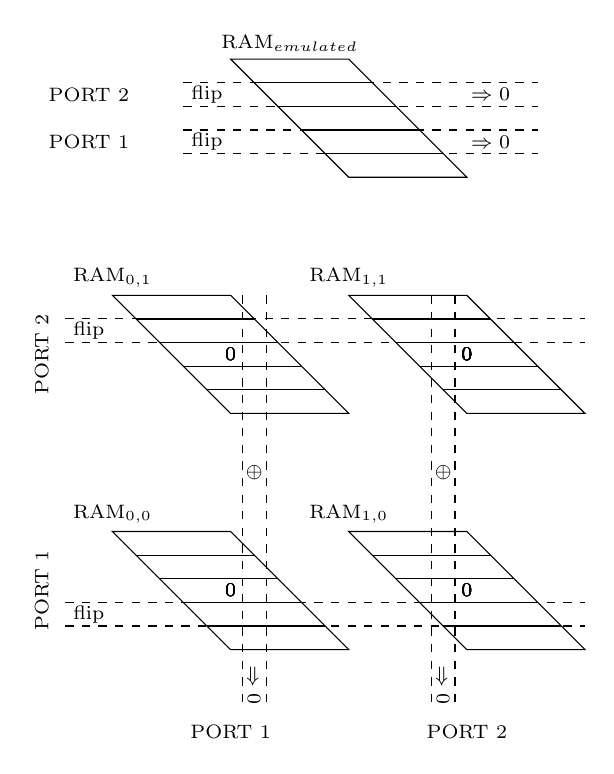
\begin{tikzpicture}[scale=3]
            \scriptsize
            \draw[] (.5,2-.25) -- (1,2-.25) -- (.5,2.25) -- (0, 2.25) -- cycle;
            \foreach \j in {-.15,-.05, .05, .15}{
                \draw[] (.25-\j, 2+\j) -- (.75-\j,2+\j);
            }
            \foreach \i/\v in {0/0,1/0,2/0,3/0,4/0}{
                \FPeval{\x}{.7-\i*.1};
                \FPeval{\y}{2-.2+\i*.1};
                \node[] at (\x,\y) {\v};
            }
            \node at (.25,2.25)[anchor=south]{RAM$_{emulated}$};
            \foreach \xram in {0,1}{
                \node at (\xram-.5,.25) [anchor=south]{RAM$_{\xram,0}$};
                \draw[xshift=\xram cm] (0,-.25) -- (.5,-.25) -- (0,.25) -- (-.5, .25) -- cycle;
                \foreach \j in {-.15,-.05, .05, .15}{
                    \draw[xshift=\xram cm] (-.25-\j, \j) -- (.25-\j,\j);
                }
                \def\y{0};
                \foreach \i/\v in {0/0,1/0,2/0,3/0,4/0}{
                    \FPeval{\x}{.2-\i*.1};
                    \FPeval{\y}{0-.2+\i*.1};
                    \node[] at (\x+\xram,\y) {\v};
                }
            }
            \foreach \xram in {0,1}{
                \node at (\xram-.5,1.25) [anchor=south]{RAM$_{\xram,1}$};
                \draw[xshift=\xram cm,yshift=1cm] (0,-.25) -- (.5,-.25) -- (0,.25) -- (-.5, .25) -- cycle;
                \foreach \j in {-.15,-.05, .05, .15}{
                    \draw[xshift=\xram cm,yshift=1cm] (-.25-\j, \j) -- (.25-\j,\j);
                }
                \def\y{0};
                \foreach \i/\v in {0/0,1/0,2/0,3/0,4/0}{
                    \FPeval{\x}{.2-\i*.1};
                    \FPeval{\y}{0-.2+\i*.1};
                    \node[] at (\x+\xram,\y+1) {\v};
                }
            }
            \node at (-.8,0)[rotate=90]{PORT 1};
            \node at (-.8,1)[rotate=90]{PORT 2};
            \node at (0,-.6){PORT 1};
            \node at (1,-.6){PORT 2};
            %TODO first and second
            \def\first{1};
            \ifthenelse{\first>0}{
            \draw[dashed] (-.7,0-.25+\first*.1) -- (1.5,0-.25+\first*.1);
            \draw[dashed] (-.7,0-.15+\first*.1) -- (1.5,0-.15+\first*.1);
            \draw[dashed] (0+.25-\first*.1,1.25) -- (0+.25-\first*.1,-.5);
            \draw[dashed] (0+.15-\first*.1,1.25) -- (0+.15-\first*.1,-.5);
            \node[rotate=270] at (0.2-\first*.1,-.4) {$\Rightarrow0$};
            \node at (0.2-\first*.1,.5) {$\oplus$};
            \node at (-.6,-.2+\first*.1) {flip};
        }{}
            \def\second{3};
            \ifthenelse{\second>0}{
            \draw[dashed] (-.7,1-.25+\second*.1) -- (1.5,1-.25+\second*.1);
            \draw[dashed] (-.7,1-.15+\second*.1) -- (1.5,1-.15+\second*.1);
            \draw[dashed] (1+.25-\second*.1,1.25) -- (1+.25-\second*.1,-.5);
            \draw[dashed] (1+.15-\second*.1,1.25) -- (1+.15-\second*.1,-.5);
            \node[rotate=270] at (1.2-\second*.1,-.4) {$\Rightarrow0$};
            \node at (1.2-\second*.1,.5) {$\oplus$};
            \node at (-.6,.8+\second*.1) {flip};
        }{}
            \ifthenelse{\first>0}{
            \draw[dashed] (-.2,2-.25+\first*.1) -- (1.3,2-.25+\first*.1);
            \draw[dashed] (-.2,2-.15+\first*.1) -- (1.3,2-.15+\first*.1);
            \node at (-.6,2-.2+\first*.1) {PORT 1};
            \node at (-.1,2-.2+\first*.1) {flip};
            \node at (1.1,2-.2+\first*.1) {$\Rightarrow0$};

        }{}
            \ifthenelse{\second>0}{
            \draw[dashed] (-.2,2-.25+\second*.1) -- (1.3,2-.25+\second*.1);
            \draw[dashed] (-.2,2-.15+\second*.1) -- (1.3,2-.15+\second*.1);
            \node at (-.6,2-.2+\second*.1) {PORT 2};
            \node at (-.1,2-.2+\second*.1) {flip};
            \node at (1.1,2-.2+\second*.1) {$\Rightarrow0$};
        }{}

        \end{tikzpicture}
        \caption{Clock Cycle}
        \label{fig:xorram0}
    \end{subfigure}
    \begin{subfigure}{.5\linewidth}
        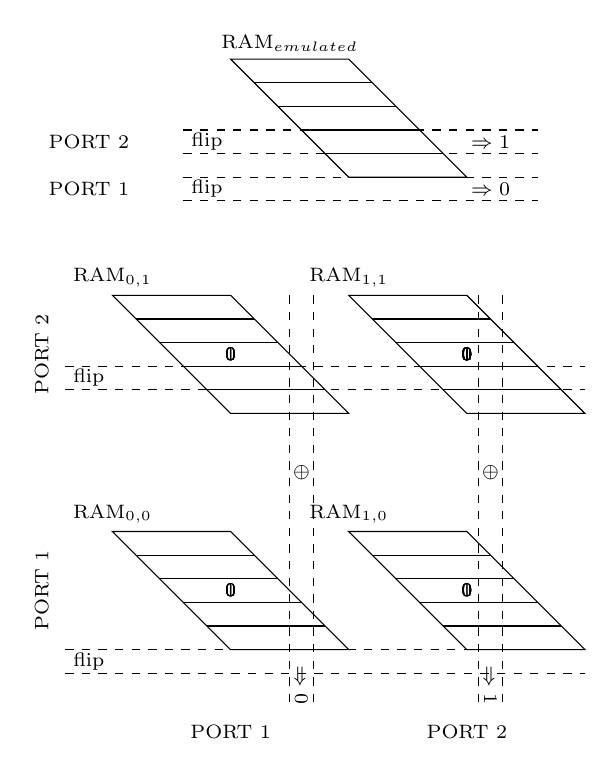
\begin{tikzpicture}[scale=3]
            \scriptsize
            \draw[] (.5,2-.25) -- (1,2-.25) -- (.5,2.25) -- (0, 2.25) -- cycle;
            \foreach \j in {-.15,-.05, .05, .15}{
                \draw[] (.25-\j, 2+\j) -- (.75-\j,2+\j);
            }
            \foreach \i/\v in {0/0,1/1,2/0,3/1,4/0}{
                \FPeval{\x}{.7-\i*.1};
                \FPeval{\y}{2-.2+\i*.1};
                \node[] at (\x,\y) {\v};
            }
            \node at (.25,2.25)[anchor=south]{RAM$_{emulated}$};
            \foreach \xram in {0,1}{
                \node at (\xram-.5,.25) [anchor=south]{RAM$_{\xram,0}$};
                \draw[xshift=\xram cm] (0,-.25) -- (.5,-.25) -- (0,.25) -- (-.5, .25) -- cycle;
                \foreach \j in {-.15,-.05, .05, .15}{
                    \draw[xshift=\xram cm] (-.25-\j, \j) -- (.25-\j,\j);
                }
                \def\y{0};
                \foreach \i/\v in {0/0,1/1,2/0,3/0,4/0}{
                    \FPeval{\x}{.2-\i*.1};
                    \FPeval{\y}{0-.2+\i*.1};
                    \node[] at (\x+\xram,\y) {\v};
                }
            }
            \foreach \xram in {0,1}{
                \node at (\xram-.5,1.25) [anchor=south]{RAM$_{\xram,1}$};
                \draw[xshift=\xram cm,yshift=1cm] (0,-.25) -- (.5,-.25) -- (0,.25) -- (-.5, .25) -- cycle;
                \foreach \j in {-.15,-.05, .05, .15}{
                    \draw[xshift=\xram cm,yshift=1cm] (-.25-\j, \j) -- (.25-\j,\j);
                }
                \def\y{0};
                \foreach \i/\v in {0/0,1/0,2/0,3/1,4/0}{
                    \FPeval{\x}{.2-\i*.1};
                    \FPeval{\y}{0-.2+\i*.1};
                    \node[] at (\x+\xram,\y+1) {\v};
                }
            }
            \node at (-.8,0)[rotate=90]{PORT 1};
            \node at (-.8,1)[rotate=90]{PORT 2};
            \node at (0,-.6){PORT 1};
            \node at (1,-.6){PORT 2};
            %TODO first and second
            \def\first{-1};
            \ifthenelse{\first>0}{
            \draw[dashed] (-.7,0-.25+\first*.1) -- (1.5,0-.25+\first*.1);
            \draw[dashed] (-.7,0-.15+\first*.1) -- (1.5,0-.15+\first*.1);
            \draw[dashed] (0+.25-\first*.1,1.25) -- (0+.25-\first*.1,-.5);
            \draw[dashed] (0+.15-\first*.1,1.25) -- (0+.15-\first*.1,-.5);
            \node[rotate=270] at (0.2-\first*.1,-.4) {$\Rightarrow 0$};
            \node at (0.2-\first*.1,.5) {$\oplus$};
            \node at (-.6,-.2+\first*.1) {flip};
        }{}
            \def\second{1};
            \ifthenelse{\second>0}{
            \draw[dashed] (-.7,1-.25+\second*.1) -- (1.5,1-.25+\second*.1);
            \draw[dashed] (-.7,1-.15+\second*.1) -- (1.5,1-.15+\second*.1);
            \draw[dashed] (1+.25-\second*.1,1.25) -- (1+.25-\second*.1,-.5);
            \draw[dashed] (1+.15-\second*.1,1.25) -- (1+.15-\second*.1,-.5);
            \node[rotate=270] at (1.2-\second*.1,-.4) {$\Rightarrow 1$};
            \node at (1.2-\second*.1,.5) {$\oplus$};
            \node at (-.6,.8+\second*.1) {flip};
        }{}
            \ifthenelse{\first>0}{
            \draw[dashed] (-.2,2-.25+\first*.1) -- (1.3,2-.25+\first*.1);
            \draw[dashed] (-.2,2-.15+\first*.1) -- (1.3,2-.15+\first*.1);
            \node at (-.6,2-.2+\first*.1) {PORT 1};
            \node at (-.1,2-.2+\first*.1) {flip};
            \node at (1.1,2-.2+\first*.1) {$\Rightarrow 0$};

        }{}
            \ifthenelse{\second>0}{
            \draw[dashed] (-.2,2-.25+\second*.1) -- (1.3,2-.25+\second*.1);
            \draw[dashed] (-.2,2-.15+\second*.1) -- (1.3,2-.15+\second*.1);
            \node at (-.6,2-.2+\second*.1) {PORT 2};
            \node at (-.1,2-.2+\second*.1) {flip};
            \node at (1.1,2-.2+\second*.1) {$\Rightarrow 1$};
        }{}

        \end{tikzpicture}
        \caption{Clock Cycle}
        \label{fig:xorram1}
    \end{subfigure}
    \begin{subfigure}{.5\linewidth}
        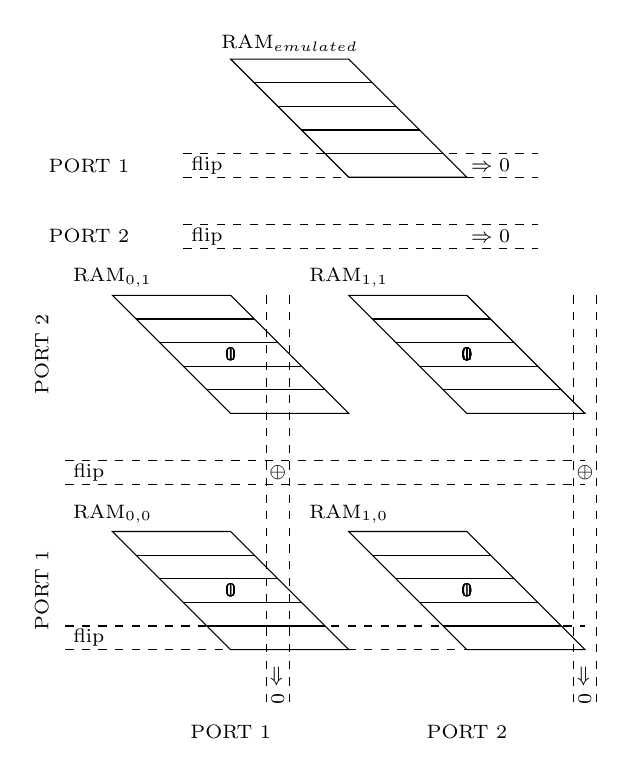
\begin{tikzpicture}[scale=3]
            \scriptsize
            \draw[] (.5,2-.25) -- (1,2-.25) -- (.5,2.25) -- (0, 2.25) -- cycle;
            \foreach \j in {-.15,-.05, .05, .15}{
                \draw[] (.25-\j, 2+\j) -- (.75-\j,2+\j);
            }
            \foreach \i/\v in {0/0,1/0,2/0,3/1,4/0}{
                \FPeval{\x}{.7-\i*.1};
                \FPeval{\y}{2-.2+\i*.1};
                \node[] at (\x,\y) {\v};
            }
            \node at (.25,2.25)[anchor=south]{RAM$_{emulated}$};
            \foreach \xram in {0,1}{
                \node at (\xram-.5,.25) [anchor=south]{RAM$_{\xram,0}$};
                \draw[xshift=\xram cm] (0,-.25) -- (.5,-.25) -- (0,.25) -- (-.5, .25) -- cycle;
                \foreach \j in {-.15,-.05, .05, .15}{
                    \draw[xshift=\xram cm] (-.25-\j, \j) -- (.25-\j,\j);
                }
                \def\y{0};
                \foreach \i/\v in {0/0,1/1,2/0,3/0,4/0}{
                    \FPeval{\x}{.2-\i*.1};
                    \FPeval{\y}{0-.2+\i*.1};
                    \node[] at (\x+\xram,\y) {\v};
                }
            }
            \foreach \xram in {0,1}{
                \node at (\xram-.5,1.25) [anchor=south]{RAM$_{\xram,1}$};
                \draw[xshift=\xram cm,yshift=1cm] (0,-.25) -- (.5,-.25) -- (0,.25) -- (-.5, .25) -- cycle;
                \foreach \j in {-.15,-.05, .05, .15}{
                    \draw[xshift=\xram cm,yshift=1cm] (-.25-\j, \j) -- (.25-\j,\j);
                }
                \def\y{0};
                \foreach \i/\v in {0/0,1/1,2/0,3/1,4/0}{
                    \FPeval{\x}{.2-\i*.1};
                    \FPeval{\y}{0-.2+\i*.1};
                    \node[] at (\x+\xram,\y+1) {\v};
                }
            }
            \node at (-.8,0)[rotate=90]{PORT 1};
            \node at (-.8,1)[rotate=90]{PORT 2};
            \node at (0,-.6){PORT 1};
            \node at (1,-.6){PORT 2};
            %TODO first and second
            \def\first{0};
            \ifthenelse{\first>-1}{
            \draw[dashed] (-.7,0-.25+\first*.1) -- (1.5,0-.25+\first*.1);
            \draw[dashed] (-.7,0-.15+\first*.1) -- (1.5,0-.15+\first*.1);
            \draw[dashed] (0+.25-\first*.1,1.25) -- (0+.25-\first*.1,-.5);
            \draw[dashed] (0+.15-\first*.1,1.25) -- (0+.15-\first*.1,-.5);
            \node[rotate=270] at (0.2-\first*.1,-.4) {$\Rightarrow 0$};
            \node at (0.2-\first*.1,.5) {$\oplus$};
            \node at (-.6,-.2+\first*.1) {flip};
        }{}
            \def\second{-3};
            \ifthenelse{\second>0}{
            \draw[dashed] (-.7,1-.25+\second*.1) -- (1.5,1-.25+\second*.1);
            \draw[dashed] (-.7,1-.15+\second*.1) -- (1.5,1-.15+\second*.1);
            \draw[dashed] (1+.25-\second*.1,1.25) -- (1+.25-\second*.1,-.5);
            \draw[dashed] (1+.15-\second*.1,1.25) -- (1+.15-\second*.1,-.5);
            \node[rotate=270] at (1.2-\second*.1,-.4) {$\Rightarrow 0$};
            \node at (1.2-\second*.1,.5) {$\oplus$};
            \node at (-.6,.8+\second*.1) {flip};
        }{}
            \ifthenelse{\first>-1}{
            \draw[dashed] (-.2,2-.25+\first*.1) -- (1.3,2-.25+\first*.1);
            \draw[dashed] (-.2,2-.15+\first*.1) -- (1.3,2-.15+\first*.1);
            \node at (-.6,2-.2+\first*.1) {PORT 1};
            \node at (-.1,2-.2+\first*.1) {flip};
            \node at (1.1,2-.2+\first*.1) {$\Rightarrow 0$};

        }{}
            \ifthenelse{\second>0}{
            \draw[dashed] (-.2,2-.25+\second*.1) -- (1.3,2-.25+\second*.1);
            \draw[dashed] (-.2,2-.15+\second*.1) -- (1.3,2-.15+\second*.1);
            \node at (-.6,2-.2+\second*.1) {PORT 2};
            \node at (-.1,2-.2+\second*.1) {flip};
            \node at (1.1,2-.2+\second*.1) {$\Rightarrow 0$};
        }{}

        \end{tikzpicture}
        \caption{Clock Cycle}
        \label{fig:xorram2}
    \end{subfigure}
    \begin{subfigure}{.5\linewidth}
        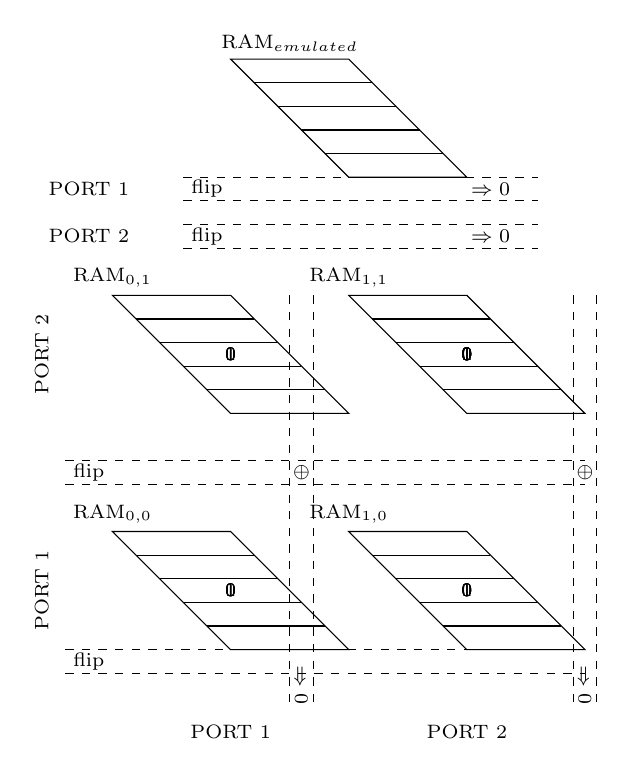
\begin{tikzpicture}[scale=3]
            \scriptsize
            \draw[] (.5,2-.25) -- (1,2-.25) -- (.5,2.25) -- (0, 2.25) -- cycle;
            \foreach \j in {-.15,-.05, .05, .15}{
                \draw[] (.25-\j, 2+\j) -- (.75-\j,2+\j);
            }
            \foreach \i/\v in {0/1,1/0,2/0,3/1,4/0}{
                \FPeval{\x}{.7-\i*.1};
                \FPeval{\y}{2-.2+\i*.1};
                \node[] at (\x,\y) {\v};
            }
            \node at (.25,2.25)[anchor=south]{RAM$_{emulated}$};
            \foreach \xram in {0,1}{
                \node at (\xram-.5,.25) [anchor=south]{RAM$_{\xram,0}$};
                \draw[xshift=\xram cm] (0,-.25) -- (.5,-.25) -- (0,.25) -- (-.5, .25) -- cycle;
                \foreach \j in {-.15,-.05, .05, .15}{
                    \draw[xshift=\xram cm] (-.25-\j, \j) -- (.25-\j,\j);
                }
                \def\y{0};
                \foreach \i/\v in {0/1,1/1,2/0,3/0,4/0}{
                    \FPeval{\x}{.2-\i*.1};
                    \FPeval{\y}{0-.2+\i*.1};
                    \node[] at (\x+\xram,\y) {\v};
                }
            }
            \foreach \xram in {0,1}{
                \node at (\xram-.5,1.25) [anchor=south]{RAM$_{\xram,1}$};
                \draw[xshift=\xram cm,yshift=1cm] (0,-.25) -- (.5,-.25) -- (0,.25) -- (-.5, .25) -- cycle;
                \foreach \j in {-.15,-.05, .05, .15}{
                    \draw[xshift=\xram cm,yshift=1cm] (-.25-\j, \j) -- (.25-\j,\j);
                }
                \def\y{0};
                \foreach \i/\v in {0/0,1/1,2/0,3/1,4/0}{
                    \FPeval{\x}{.2-\i*.1};
                    \FPeval{\y}{0-.2+\i*.1};
                    \node[] at (\x+\xram,\y+1) {\v};
                }
            }
            \node at (-.8,0)[rotate=90]{PORT 1};
            \node at (-.8,1)[rotate=90]{PORT 2};
            \node at (0,-.6){PORT 1};
            \node at (1,-.6){PORT 2};
            %TODO first and second
            \def\first{-1};
            \ifthenelse{\first>0}{
            \draw[dashed] (-.7,0-.25+\first*.1) -- (1.5,0-.25+\first*.1);
            \draw[dashed] (-.7,0-.15+\first*.1) -- (1.5,0-.15+\first*.1);
            \draw[dashed] (0+.25-\first*.1,1.25) -- (0+.25-\first*.1,-.5);
            \draw[dashed] (0+.15-\first*.1,1.25) -- (0+.15-\first*.1,-.5);
            \node[rotate=270] at (0.2-\first*.1,-.4) {$\Rightarrow 0$};
            \node at (0.2-\first*.1,.5) {$\oplus$};
            \node at (-.6,-.2+\first*.1) {flip};
        }{}
            \def\second{-3};
            \ifthenelse{\second>0}{
            \draw[dashed] (-.7,1-.25+\second*.1) -- (1.5,1-.25+\second*.1);
            \draw[dashed] (-.7,1-.15+\second*.1) -- (1.5,1-.15+\second*.1);
            \draw[dashed] (1+.25-\second*.1,1.25) -- (1+.25-\second*.1,-.5);
            \draw[dashed] (1+.15-\second*.1,1.25) -- (1+.15-\second*.1,-.5);
            \node[rotate=270] at (1.2-\second*.1,-.4) {$\Rightarrow 0$};
            \node at (1.2-\second*.1,.5) {$\oplus$};
            \node at (-.6,.8+\second*.1) {flip};
        }{}
            \ifthenelse{\first>0}{
            \draw[dashed] (-.2,2-.25+\first*.1) -- (1.3,2-.25+\first*.1);
            \draw[dashed] (-.2,2-.15+\first*.1) -- (1.3,2-.15+\first*.1);
            \node at (-.6,2-.2+\first*.1) {PORT 1};
            \node at (-.1,2-.2+\first*.1) {flip};
            \node at (1.1,2-.2+\first*.1) {$\Rightarrow 0$};

        }{}
            \ifthenelse{\second>0}{
            \draw[dashed] (-.2,2-.25+\second*.1) -- (1.3,2-.25+\second*.1);
            \draw[dashed] (-.2,2-.15+\second*.1) -- (1.3,2-.15+\second*.1);
            \node at (-.6,2-.2+\second*.1) {PORT 2};
            \node at (-.1,2-.2+\second*.1) {flip};
            \node at (1.1,2-.2+\second*.1) {$\Rightarrow 0$};
        }{}

        \end{tikzpicture}
        \caption{Clock Cycle}
        \label{fig:xorram3}
    \end{subfigure}
    \caption{The operation of the clever architecture.}
    \label{fig:xorram}
\end{figure}

%%\chapter{SPARSE MATRIX COMPRESSION}
\label{chp:compression}

Although we address this pillar last we view it as the most important. We previously implemented matrix compression in \cite{prelim:townsend}. However, we made the mistake of combining the two types of compression, index and floating point into one scheme. This simplified some aspects of the design. For example, this compression only needed to keep track of one data stream. Combining the two parts also makes sense if the two are correlated. In the extreme case the values in matrix could be calculated from the indices. However, we do not see an easy way to use this for general sparse matrix compression.

This chapter is dedicated to sprase pattern matrix compression, which we call SMC. In the next chapter we disscuss our floating point compression, which we call fzip. This chapter starts with Section~\ref{sec:index_compression_related_work} discussing related work. Then, Section~\ref{sec:index_compression_analysis} discusses the analysis of delta compression. Then, Section~\ref{sec:smc} discusses our implementation. Then, Section~\ref{sec:smc_decoder} discusses the hardware decorder for SMC. Lastly, Section~\ref{sec:smc_discussion} discusses something.

\section{Related Work}
\label{sec:index_compression_related_work}
Some work exists on compressing indices beyond coordinate (COO) format. The most obvious one and the one mentioned back in Chapter~\ref{chp:background} is compressed sparse row (CSR) format. The majority of work on computing SpMV on FPGAs uses CSR [\cite{prelim:nagar1}]. However we did find one alternative that uses a format called CVBV [\cite{prelim:kestur}]. Also, \cite{prelim:kourtis} uses index compression to speed up their CPU implementation. In addition to these we also look at how well gzip can compress indices.

Since both CVBV and the CPU method benefit from our RCR traversal we use that when analyzing them rather than row major traversal.
\subsection{CVBV}

Compressed Variable Bit Vector (CVBV) is a format created by [\cite{prelim:kestur}]. This implementation has two streams, which we will call the code stream and the argument stream. The code stream stores one 4 bit code for each delta. The first bit indicates what the type of the code is, dense (1) or regular (0). If the bit equals 1 (a dense code type) then the delta equals 1 and the value in the argument indicates how many deltas equal to 1 follow. If the bit equals 0 (a regular code type) then the delta equals the value in the argument.

The other 3 bits indicate how many nibbles are in the argument. The argument is taken from the argument stream. The results of this implementation is in Table~\ref{tbl:index} column 4.
\subsection{CPU method}

The method in [\cite{prelim:kourtis}] is similar but targeted for CPUs rather than FPGAs. Again there are 2 streams a code stream and an argument stream. The codes are 2 bytes long. Instead of one code per delta there is one code per array of deltas. The first byte indicates what size the deltas are, 1, 2, 4, or 8 bytes, and in the array is the last one in the row. The second byte indicates the length of the array.

The argument stream can be padded to make sure the data types align properly. The whole propose of this implementation is that nat\"ive data types are used so the CPU can process them faster. The compression results of this implementation is in Table~\ref{tbl:index} column 5.

\subsection{gzip}
We also choose to use the general compression program gzip in the comparison as well. Table~\ref{tbl:index} shows the compression of gzip on top of the CSR format. gzip does very well, partly because column indicies ofeten repeat.


\begin{table*}
\centering
\begin{threeparttable}
    \caption[Detailed analysis of index compression.]{This table shows the number of bytes per non-zero value the given index compression scheme achieves. (No floating point values are being compressed here.)}
\label{tbl:index}
\begin{tabular}{cccccccc}
\hline
\bfseries Matrix & \bfseries \tikz \node[rotate=90]{COO}; & \bfseries \tikz \node[rotate=90]{CSR}; & \bfseries \tikz \node[rotate=90]{CSR.gz}; & \bfseries \tikz \node[rotate=90]{cvbv}; & \bfseries \tikz \node[rotate=90]{cpu}; & \bfseries \tikz \node[rotate=90]{smc}; & \bfseries \tikz \node [rotate=90]{smc.gz};  \\
\hline
cant & 8.00 & 4.06 & 0.40 & 0.51 & 1.01 & 0.26 & 0.04 \\
consph & 8.00 & 4.06 & 0.19 & 0.45 & 1.01 & 0.26 & 0.03 \\
cop20k\_A & 8.00 & 4.18 & 1.07 & 0.99 & 1.01 & 0.64 & 0.54 \\
dense2 & 8.00 & 4.00 & 0.03 & 0.00 & 1.01 & 0.13 & 0.00 \\
mac\_econ\_fwd500 & 8.00 & 4.65 & 1.48 & 1.32 & 1.01 & 0.91 & 0.48 \\
mc2depi & 8.00 & 5.00 & 1.78 & 1.12 & 1.01 & 0.41 & 0.02 \\
pdb1HYS & 8.00 & 4.03 & 0.14 & 0.24 & 1.01 & 0.20 & 0.07 \\
pwtk & 8.00 & 4.07 & 0.16 & 0.23 & 1.01 & 0.19 & 0.01 \\
qcd5\_4 & 8.00 & 4.10 & 0.31 & 0.62 & 1.01 & 0.28 & 0.01 \\
rail4284 & 8.00 & 4.00 & 1.41 & 0.62 & 1.01 & 0.50 & 0.45 \\
rma10 & 8.00 & 4.08 & 0.20 & 0.38 & 1.01 & 0.24 & 0.09 \\
scircuit & 8.00 & 4.71 & 1.61 & 1.11 & 1.01 & 0.76 & 0.61 \\
shipsec1 & 8.00 & 4.07 & 0.20 & 0.45 & 1.01 & 0.22 & 0.06 \\
webbase-1M & 8.00 & 5.29 & 1.35 & 1.09 & 1.01 & 0.58 & 0.31 \\
\hline
average\tnote{a} & 8.00 & 4.33 & 0.79 & 0.70 & 1.01 & 0.42 & 0.21\\

\hline
\end{tabular}
\begin{tablenotes}
\item [a] Excludes the dense matrix.
\end{tablenotes}
\end{threeparttable}
\end{table*}

\section{Analysis}
\label{sec:index_compression_analysis}

We did some analysis on the distribution of deltas to come up with our implementation. The most important analysis was the distribution of delta lengths Table~\ref{tbl:index}. This table show the distribution of deltas for the RCR traversal. In this case we set the subwidth to 8 and the subheight to 512. There are some key characteristics to notice. First, about half of the deltas equal 1. Second, on average less than 5\% of the deltas are more than 512. Third, with some eye squinting the frequency distribution of the deltas is approximately a decreasing exponential.

\begin{sidewaystable}
\centering
\begin{threeparttable}
    \caption[The distribution of deltas by bit length.]{The distribution of the bit lengths required to store the delta length when using RCR traversal with the subheight set to 512 and the subwidth set to 8.}
\label{tbl:indexDist}
\begin{tabular}{cccccccccccc}
\hline
\bfseries Matrix & \bfseries 1 & \bfseries 2 & \bfseries 3-4 & \bfseries 5-8 & \bfseries 9-16 & \bfseries 17-32 & \bfseries 33-64 &\bfseries 65-128 & \bfseries 129-256 & \bfseries 257-512 & \bfseries 512+\\
\hline
cant & 72.2\% & 6.3\% & 6.8\% & 12.3\% & 0.7\% & 0.0\% & 0.0\% & 1.0\% & 0.0\% & 0.0\% & 0.6\% \\
consph & 76.6\% & 3.1\% & 5.9\% & 11.6\% & 0.8\% & 0.0\% & 0.0\% & 0.0\% & 0.1\% & 1.0\% & 0.8\% \\
cop20k\_A & 51.1\% & 1.9\% & 3.2\% & 22.9\% & 2.4\% & 1.0\% & 1.0\% & 1.0\% & 0.8\% & 0.7\% & 14.0\% \\
dense2 & 100.0\% & 0.0\% & 0.0\% & 0.0\% & 0.0\% & 0.0\% & 0.0\% & 0.0\% & 0.0\% & 0.0\% & 0.0\% \\
mac\_econ\_fwd500 & 8.2\% & 7.8\% & 7.3\% & 19.0\% & 12.0\% & 15.2\% & 6.3\% & 5.1\% & 2.8\% & 7.1\% & 9.2\% \\
mc2depi & 21.8\% & 0.0\% & 0.0\% & 24.9\% & 43.8\% & 0.0\% & 0.0\% & 0.0\% & 0.0\% & 0.1\% & 9.4\% \\
pdb1HYS & 88.0\% & 1.1\% & 3.6\% & 5.9\% & 0.0\% & 0.3\% & 0.2\% & 0.2\% & 0.1\% & 0.1\% & 0.4\% \\
pwtk & 87.7\% & 2.7\% & 3.0\% & 5.8\% & 0.0\% & 0.0\% & 0.0\% & 0.0\% & 0.0\% & 0.0\% & 0.8\% \\
qcd5\_4 & 66.0\% & 0.0\% & 8.2\% & 19.7\% & 3.6\% & 0.0\% & 0.0\% & 0.2\% & 0.0\% & 0.2\% & 2.1\% \\
rail4284 & 71.2\% & 1.0\% & 1.5\% & 5.3\% & 0.4\% & 1.0\% & 1.5\% & 1.5\% & 1.6\% & 2.0\% & 12.9\% \\
rma10 & 80.6\% & 1.4\% & 6.5\% & 8.8\% & 0.2\% & 0.8\% & 0.3\% & 0.1\% & 0.1\% & 0.2\% & 0.9\% \\
scircuit & 35.3\% & 2.8\% & 3.2\% & 25.7\% & 8.0\% & 3.5\% & 2.7\% & 2.3\% & 1.6\% & 1.1\% & 13.7\% \\
shipsec1 & 78.4\% & 0.0\% & 6.1\% & 12.2\% & 1.1\% & 0.0\% & 0.3\% & 0.2\% & 0.3\% & 0.2\% & 1.3\% \\
webbase-1M & 14.6\% & 3.5\% & 2.3\% & 37.7\% & 28.7\% & 1.0\% & 0.8\% & 0.5\% & 0.4\% & 0.4\% & 10.1\% \\
\hline
average\tnote{a} & 57.8\% & 2.4\% & 4.4\% & 16.3\% & 7.8\% & 1.8\% & 1.0\% & 0.9\% & 0.6\% & 1.0\% & 5.9\% \\
\hline
\end{tabular}
\begin{tablenotes}
\item [a] Excludes dense matrix
\end{tablenotes}
\end{threeparttable}
\end{sidewaystable}%

\section{Sparse Pattern Matrix Compression (SMC)}
\label{sec:smc}
We approach the problem of how to encode the series of deltas by giving each delta a code. We also created a special new line code. However, there are too many delta lengths to give each one a unique code. So we have 3 types of codes:
\begin{enumerate}
    \item Constant offset code.
    \item Variable offset code.
    \item New line code.
\end{enumerate}

The constant offset codes represent small deltas and decode as the exact value of the delta. The valiable offset codes represent larger deltas and decode as the bit length of the delta ($\textrm{log}_2(\delta)$). The new line codes represent the end of the 512 row section. After a newline code is read the running `major' row index will increment and the running `minor' row index will reset to -1 and all of the running column index will reset to -1.

Based on the analysis in Table~\ref{tbl:indexDist} we choose to have 32 constant offset codes. Using the deltas we can determine the frquencies of each code. With these frequencies we can create the codes using Huffman encoding [\cite{prelim:huffman}].

As an example, consider the example matrix back in Chapter~\ref{chp:background} in Equation~\ref{eqn:example}. Using row-major traversal (rather than RCR traversal) the deltas are:\\
1, 3, 3, \textbackslash n, 5, 3, \textbackslash n, 2, 1, 3, 1, \textbackslash n, 1, 4, \textbackslash n, 3, 1, 3, 1, \textbackslash n, 2, 3, \textbackslash n, 2, 1, 3, 2, \textbackslash n, 3, 1, 1, 1

Using 2 (rather than 32) constant offsets, the codes and their frequencies are:\\
\begin{enumerate}
    \item 1 : 10
    \item 2 : 4
    \item 3-4 : 9
    \item 5-8 : 1
    \item \textbackslash n : 7
\end{enumerate}
This results in 5 codes: 2 constant offset codes, 2 variable offsets codes, and 1 newline code. Now these codes are given varible length codes through Huffman encoding.

Huffman encoding first creates a huffman tree, which then is used to create the codes. The tree is created as follows. First, create a lone node for each code. Second, sort the nodes by frequency. Third, pop the two nodes with the lowest frequency from the list, and make the two nodes children of a new node. Fourth, set the frequency value of this new node to the sum of the frquencies of the children. Fifth, insert the new node back into the sorted list. Then repeat the third through fifth steps until the list only contains one node. \figurename~\ref{fig:huffman_tree} shows the creation of the Huffman tree. The following is the sorted list at each iteration:
\begin{enumerate}
    \item (1 : 10), (3-4 : 9), (\textbackslash n : 7), (2 : 4), (5-8 : 1)
    \item (1 : 10), (3-4 : 9), (\textbackslash n : 7), (a : 5)
    \item (b : 12), (1 : 10), (3-4 : 9)
    \item (c : 19), (b : 12)
    \item (d : 31)
\end{enumerate}
\begin{figure}
    \begin{subfigure}{.2\linewidth}
        \centering
        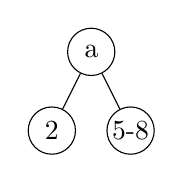
\begin{tikzpicture}
            \node(a)[circle,draw,inner sep=0pt,minimum size=.6cm] at (0,0){a};
            \node(2)[circle,draw,inner sep=0pt,minimum size=.6cm] at (-.5,-1){2};
            \node(58)[circle,draw,inner sep=0pt,minimum size=.6cm] at (.5,-1){5-8};
            \draw (a) -- (2);
            \draw (a) -- (58);
        \end{tikzpicture}
        \caption{Added `a'}
        \label{fig:Huffmantree1}
    \end{subfigure}
    \begin{subfigure}{.2\linewidth}
        \centering
        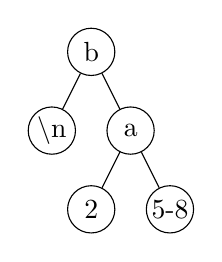
\begin{tikzpicture}
            \node(n)[circle,draw,inner sep=0pt,minimum size=.6cm] at (-1,0){\textbackslash n};
            \node(b)[circle,draw,inner sep=0pt,minimum size=.6cm] at (-.5,1){b};
            \node(a)[circle,draw,inner sep=0pt,minimum size=.6cm] at (0,0){a};
            \node(2)[circle,draw,inner sep=0pt,minimum size=.6cm] at (-.5,-1){2};
            \node(58)[circle,draw,inner sep=0pt,minimum size=.6cm] at (.5,-1){5-8};
            \draw (a) -- (2);
            \draw (a) -- (58);
            \draw (b) -- (n);
            \draw (b) -- (a);
        \end{tikzpicture}
        \caption{Added `b'}
        \label{fig:Huffmantree2}
    \end{subfigure}
    \begin{subfigure}{.5\linewidth}
        \centering
        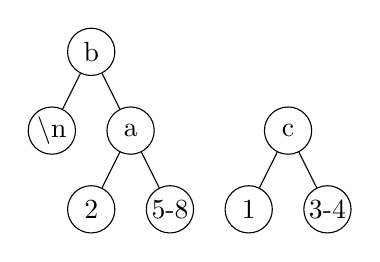
\begin{tikzpicture}
            \node(n)[circle,draw,inner sep=0pt,minimum size=.6cm] at (-1,0){\textbackslash n};
            \node(b)[circle,draw,inner sep=0pt,minimum size=.6cm] at (-.5,1){b};
            \node(a)[circle,draw,inner sep=0pt,minimum size=.6cm] at (0,0){a};
            \node(2)[circle,draw,inner sep=0pt,minimum size=.6cm] at (-.5,-1){2};
            \node(58)[circle,draw,inner sep=0pt,minimum size=.6cm] at (.5,-1){ 5-8 };
            \node(1)[circle,draw,inner sep=0pt,minimum size=.6cm] at (1.5,-1){ 1 };
            \node(34)[circle,draw,inner sep=0pt,minimum size=.6cm] at (2.5,-1){ 3-4 };
            \node(c)[circle,draw,inner sep=0pt,minimum size=.6cm] at (2,0){c};
            \draw (a) -- (2);
            \draw (a) -- (58);
            \draw (b) -- (n);
            \draw (b) -- (a);
            \draw (c) -- (1);
            \draw (c) -- (34);
        \end{tikzpicture}
        \caption{Added `c'}
        \label{fig:Huffmantree3}
    \end{subfigure}
    \begin{subfigure}{.45\linewidth}
        \centering
        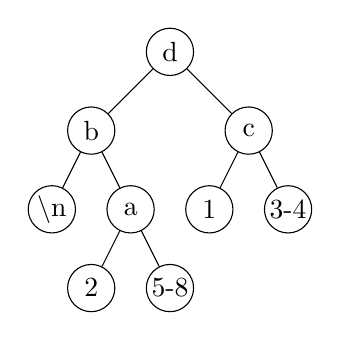
\begin{tikzpicture}
            \node(n)[circle,draw,inner sep=0pt,minimum size=.6cm] at (-1,0){\textbackslash n};
            \node(b)[circle,draw,inner sep=0pt,minimum size=.6cm] at (-.5,1){b};
            \node(a)[circle,draw,inner sep=0pt,minimum size=.6cm] at (0,0){a};
            \node(2)[circle,draw,inner sep=0pt,minimum size=.6cm] at (-.5,-1){2};
            \node(58)[circle,draw,inner sep=0pt,minimum size=.6cm] at (.5,-1){ 5-8 };
            \node(1)[circle,draw,inner sep=0pt,minimum size=.6cm] at (1,0){ 1 };
            \node(34)[circle,draw,inner sep=0pt,minimum size=.6cm] at (2,0){ 3-4 };
            \node(c)[circle,draw,inner sep=0pt,minimum size=.6cm] at (1.5,1){c};
            \node(d)[circle,draw,inner sep=0pt,minimum size=.6cm] at (.5,2){d};
            \draw (a) -- (2);
            \draw (a) -- (58);
            \draw (b) -- (n);
            \draw (b) -- (a);
            \draw (c) -- (1);
            \draw (c) -- (34);
            \draw (d) -- (b);
            \draw (d) -- (c);
        \end{tikzpicture}
        \caption{Added `d'}
        \label{fig:Huffmantree3}
    \end{subfigure}
    \caption{trees}
    \label{fig:huffman_tree}
\end{figure}

To encode a large delta with a variable length code, the delta (minus the most significant bit) is pushed onto an argument stream. In the end the SMC file has three parts: the header, the dictionary, the codes stream, and the argument stream.

To make decoding easier we set the maximum code length to 9. We do this by artificially increasing the frequency of each code to a minimum of $\frac{nnz}{2^9}$. In the SMC file a code dictionary needs to be present so that the file can be decompressed. For easier decoding we have $2^9$ records with all the information to decode them.

\section{The SMC decoder}
\label{sec:smc_decoder}
The hardware decoder relies on lookup tables to decode the two streams (see \figurename~\ref{fig:smc_decoder}). First the dictonary is loaded onto a large 512 value lookup table (LUT). This lookup table uses the code length to determine how much to right shift the first shift buffer. The LUT then determines if the second shift buffer is needed (the code is a variable length delta). In that case, the second shift buffer is right shifted and the output is used to create the delta. Then the delta (or newline) is sent to the running row and column index and the current row and column index is outputed from the decoder.
\begin{figure}
    \centering
    \begin{tikzpicture}
        \node at (0,1) {Memory};
        \node at (4,1) {Decoder};
        \draw [dashed](1.5,1.5) -- (1.5,-4);
        \node at (0,0)[draw,trapezium,trapezium right angle=120,trapezium left angle=60](h){Header};
        \node at (0,-1)[draw,trapezium,trapezium right angle=120,trapezium left angle=60](d){Dictionary};
        \node at (0,-2.2)[draw,trapezium,trapezium right angle=120,trapezium left angle=60](ds){\shortstack{Data\\Stream}};
        \node at (0,-3.6)[draw,trapezium,trapezium right angle=120,trapezium left angle=60](as){\shortstack{Argument\\Stream}};

        \node at (4, 0) [draw,minimum width=4cm](sb1){Shifter Buffer};
        \node at (2.5, -1.5) [draw,minimum height=1cm](l){LUT};
        \node at (4, -3) [draw,minimum width=4cm](sb2){Shifter Buffer};
        \node at (5.5, -1.5) [draw,minimum height=1cm](dti){\shortstack{Delta to\\Index}};
        \node at (7, -1)(r){row};
        \node at (7, -2)(c){col};

        \draw[->,shorten >=2pt] (ds) .. controls ++(1.5,0)  and ++(-2.5,0) .. (sb1);
        \draw[->,shorten >=2pt] (sb1.350) .. controls ++(0,-.5) and ++(0,.5) .. (l.north -| 2.6,0);
        \draw[<-,shorten <=2pt] (sb1.south -| 2.4,0) .. controls ++(0,-.5) and ++(0,.5) .. (l.north -| 2.3,0);
        \draw[->,shorten >=2pt] (as) .. controls ++(1.5,0) and ++(-2.5,0) .. (sb2);
        \draw[->,shorten >=2pt] (l) -- (l|-sb2.north);
        %\draw (l) |- (sb2);
        \draw[->,shorten >=2pt] (sb2.10) .. controls ++(0,.5) and ++(-1,0) .. (4,-1.5);
        \draw[->,shorten >=2pt] (d) .. controls ++(1.5,0) and ++(-1,0) .. (l);
        \draw[->,shorten >=2pt] (l) -- (dti);
        \draw[->,shorten >=2pt] (dti) -- (r);
        \draw[->,shorten >=2pt] (dti) -- (c);

    \end{tikzpicture}
    \caption{The hardware design of the SMC decoder.}
    \label{fig:smc_decoder}
\end{figure}

We do not have the exact area and performance of this decoder because we only designed a decoder that combined the index and floating point decoding. However, the first shift buffer uses 293 LUTs and 60 registers. The second shift buffer uses 469 LUTs and 82 registers. The combined decoder has a top frequency of 150 Mhz after place and route using xst.

\section{Results}
\label{sec:smc_discussion}

Table~\ref{tbl:index}  shows the results of SMC compression. As seen, it outperforms the pervious implementations. In addition, we looked at compressing the smc file further with gzip. This achieve a good deal of addition compression. One reason for this additional compression is that it compresses the repeating deltas equal to 1 in the dense sections of the matrix.

%%\chapter{FLOATING POINT COMPRESSION}
\label{chp:fzip}
\newif\ifshort

%\shortfalse
%or
\shorttrue

\newif\ifbwtsec

\bwtsecfalse
%\bwtsectrue
Floating point compression is the second half of matrix compression. \figurename~\ref{tbl:value} shows a comparison of compression schemes. In the end, we created a program and library called fzip. In total, fzip takes advantage of 2 compressible features of datasets: repeating values (patterns exactly 8 bytes long), and repeating prefixes (patterns less than 8 bytes long). For SpMV, we need to make a hardware decoder. So taking advantage of sequences that are more than 8 bytes long is difficult. In the remainder of this chapter we talk about an analysis of floating point datasets (Section \ref{sec:fzipanalysis}), our approach to floating point compression (Section \ref{sec:fzipapproach}), our hardware decoder (Section~\ref{sec:fzip_decoder}) and our results (Section \ref{sec:fzipdiscussion}).

\begin{table*}
\centering
\begin{threeparttable}
    \caption[Value compression analysis.]{Detailed value compression analysis and performance comparison, in terms of bytes per non-zero value.}
\label{tbl:value}
\begin{tabular}{ccccccccc}
\hline
\bfseries Matrix & \bfseries \tikz \node[rotate=90]{uncompressed}; & \bfseries \tikz \node[rotate=90]{Unique Values}; & \bfseries \tikz \node[rotate=90]{Unique/nnz $\times 8$}; & \bfseries \tikz \node[rotate=90]{256 Common}; & \bfseries \tikz \node[rotate=90]{GZIP}; & \bfseries \tikz \node[rotate=90]{FPC};\\
\hline
dense2\tnote{a} & $8.00$ & $1.00$ & $0.00$ & $1.00$ & $0.01$ & $0.50$ \\
pdb1HYS & $8.00$ & $1.10 \times 10^{6}$ & $4.08$ & $7.99$ & $4.15$ & $7.99$  \\
consph & $8.00$ & $1.24 \times 10^{6}$ & $3.28$ & $7.99$ & $5.10$ & $7.95$  \\
cant & $8.00$ & $1.07 \times 10^{2}$ & $0.00$ & $1.00$ & $0.11$ & $0.91$  \\
pwtk & $8.00$ & $3.63 \times 10^{6}$ & $5.04$ & $7.95$ & $4.29$ & $7.37$  \\
rma10\tnote{a} & $8.00$ & $1.00$ & $0.00$ & $1.00$ & $0.01$ & $0.50$  \\
qcd5\_4\tnote{a} & $8.00$ & $1.00$ & $0.00$ & $1.00$ & $0.01$ & $0.50$  \\
shipsec1 & $8.00$ & $8.86 \times 10^{4}$ & $0.56$ & $6.39$ & $2.08$ & $3.80$ \\
mac\_econ\_fwd500 & $8.00$ & $1.08 \times 10^{5}$ & $1.36$ & $5.20$ & $0.73$ & $1.45$ \\
mc2depi & $8.00$ & $3.58 \times 10^{3}$ & $0.00$ & $4.94$ & $1.24$ & $5.01$ \\
cop20k\_A & $8.00$ & $9.56 \times 10^{5}$ & $5.84$ & $7.97$ & $5.53$ & $7.97$ \\
scircuit & $8.00$ & $8.82 \times 10^{4}$ & $1.44$ & $5.41$ & $1.95$ & $3.68$ \\
webbase-1M & $8.00$ & $5.65 \times 10^{2}$ & $0.00$ & $1.48$ & $0.38$ & $1.92$ \\
\hline
average\tnote{b} & $8.00$ & $7.22 \times 10^{5}$ & $2.16$ & $5.63$ & $2.56$ & $4.81$ \\

\hline
\end{tabular}
\begin{tablenotes}
\item [a] Boolean matrices
\item [b] Excludes boolean matrices
\end{tablenotes}
\end{threeparttable}
\end{table*}
%
\section{Related Work}
\label{sec:fziprelated}
It was noted in \cite{prelim:kourtis, prelim:grigoras} that sparse matrices often have repeated values. This is the focus of our value compression. Our previous work ($R^3$) had a simple scheme using this feature. It stored the 256 most common values so those common values could be represented as one byte. The performance of this scheme is shown in the column ``256 common" in Table~\ref{tbl:value}.\par
We analyze gzip, bzip and FPC [\cite{prelim:burtscher}] to see how high a compression ratio over the uncompressed 8 bytes per value is achievable.\par
Uncompressed data would take 8 bytes per element. Any good compression scheme should take less than 8 bytes per element. We looked at \cite{prelim:burtscher} describing its own compression scheme, FPC. This scheme looks for repeated patterns. However it does not exploit the fact most of its compression comes from exact (8 byte) value repeats. To illustrate this point we created an ``anti-FPC" dataset (\figurename~\ref{fig:antiFpc}).
\begin{figure}
    \center
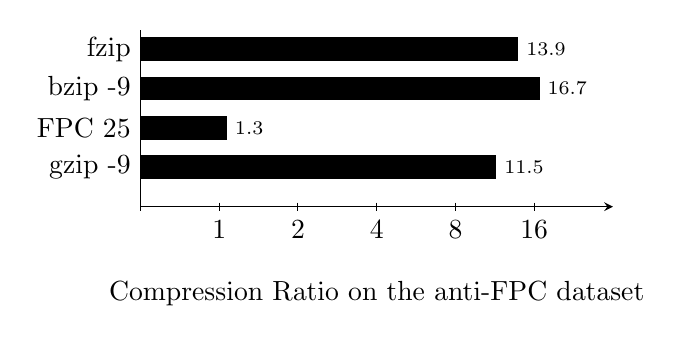
\begin{tikzpicture}[yscale=.5]
\draw (0,0) -- (0,4.5);
\draw[-stealth] (0,0) -- (6,0);
\foreach \x/\n in {0/,1/1,2/2,3/4,4/8,5/16}{
    \draw (\x,.1) -- (\x,-.1)node[anchor=north]{\n};
}
\node at (3,-2.2){Compression Ratio on the anti-FPC dataset};
\foreach \y/\n in {0/,1/gzip -9,2/FPC 25,3/bzip -9,4/fzip}{
    \node[anchor=east, rotate=0] at (0,\y){\n};
}
\scriptsize
\foreach \x/\y/\n in {4.52/1/11.5,1.1/2/1.3,5.07/3/16.7,4.8/4/13.9}{
    \fill (0,\y-.3) rectangle (\x,\y+.3);
    \node[anchor=west] at (\x,\y){\n};
}
\end{tikzpicture}
\caption[The Anti-FPC dataset]{We engineering a dataset to make the performance of FPC look bad compared to other programs. Although unfair, this shows a type of pattern that FPC does not exploit and other programs do. This problem exists because FPC only uses predictors for compression.}
\label{fig:antiFpc}
\end{figure}

\par gzip performs quite well too. We have a general understanding of how gzip works. We suspect the reason for the good performance is the large memory space and being able to look up previously occurring 8-byte values.
\par Our focus on using repeated values is reinforced by looking at the number of unique values. If only the unique values were stored the average compression would be $2.16$ bytes per element. This can not be used by itself since this ignores the indexing required to access these values, but this gives an estimate of the possible compression size.
\begin{figure}
\center
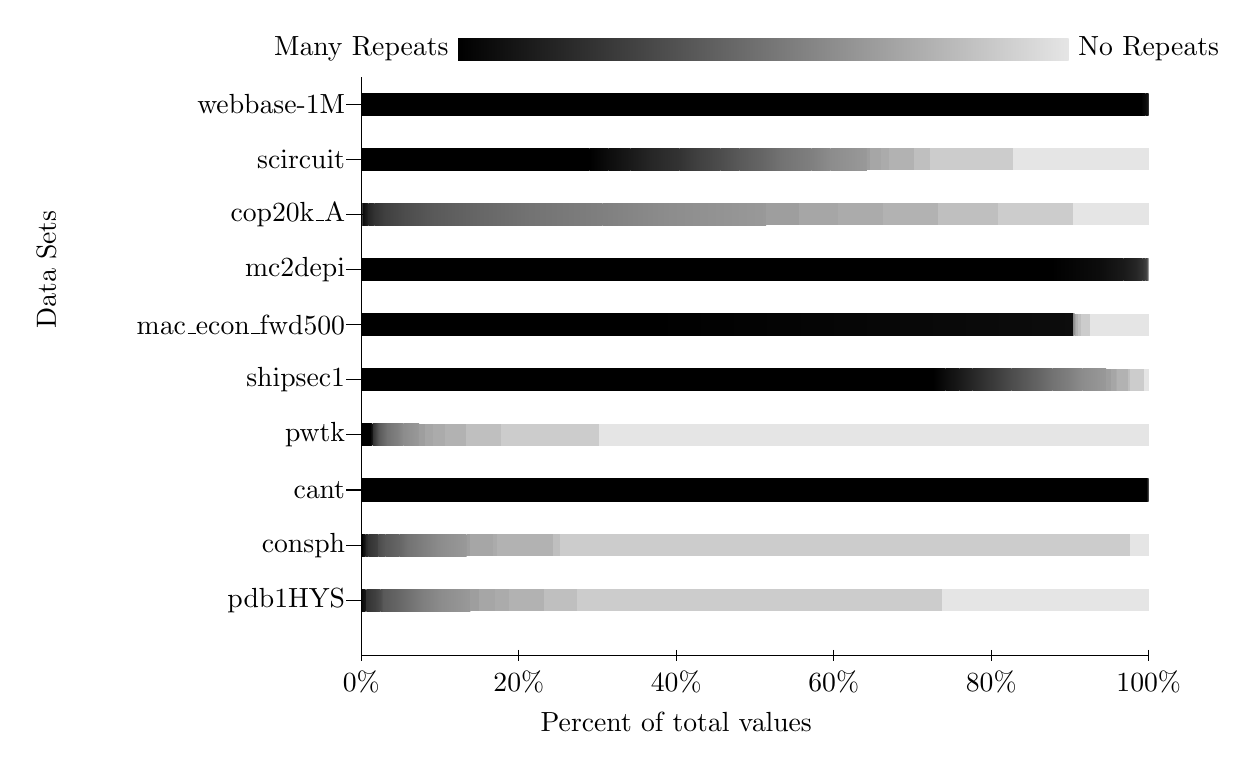
\begin{tikzpicture}[yscale=.7,xscale=2]

\path[draw] (0,0) -- (0,10.5);
\path[draw] (0,0) -- (5,0);
\foreach \x/\v in {0/0,1/20,2/40,3/60,4/80,5/100}{
    \draw (\x,.1) -- (\x,-.1)node[anchor=north]{\v\%};
}

\foreach \n/\y in {pdb1HYS/1, consph/2, cant/3, pwtk/4, shipsec1/5, mac\_econ\_fwd500/6, mc2depi/7, cop20k\_A/8, scircuit/9, webbase-1M/10}{
    \draw (.1,\y) -- (-.1,\y)node[anchor=east,rotate=0,inner sep=0]{\n};
}
\node at (2,-1.2){Percent of total values};
\node[rotate=90] at (-2,7){Data Sets};

%pdb1HYS
\foreach \xa/\xb/\sa/\sb in {0/0.00457/100/100,0.00457/0.00531/100/95,0.00531/0.0281/95/90,0.0281/0.0313/90/85,0.0313/0.0327/85/80,0.0327/0.0879/80/75,0.0879/0.123/75/70,0.123/0.139/70/65,0.139/0.234/65/60,0.234/0.314/60/55,0.314/0.398/55/50,0.398/0.507/50/45,0.507/0.692/45/40,}{
    \shade[left color=black!\sa,right color=black!\sb] (\xa,0.8) rectangle (\xb,1.2);
}
\foreach \xa/\xb/\s in {0.692/0.748/38,0.748/0.847/35,0.847/0.939/33,0.939/1.16/30,1.16/1.37/25,1.37/3.69/20,3.69/5/10}{
    \fill[black!\s] (\xa,0.8) rectangle (\xb,1.2);
}
%consph
\foreach \xa/\xb/\sa/\sb in {0/0.00387/100/100,0.00387/0.0118/100/95,0.0118/0.0268/95/90,0.0268/0.0274/90/85,0.0274/0.0464/85/80,0.0464/0.0992/80/75,0.0992/0.11/75/70,0.11/0.154/70/65,0.154/0.242/65/60,0.242/0.295/60/55,0.295/0.398/55/50,0.398/0.5/50/45,0.5/0.668/45/40,}{
    \shade[left color=black!\sa,right color=black!\sb] (\xa,1.8) rectangle (\xb,2.2);
}
\foreach \xa/\xb/\s in {0.668/0.689/38,0.689/0.834/35,0.834/0.86/33,0.86/1.22/30,1.22/1.26/25,1.26/4.88/20,4.88/5/10}{
    \fill[black!\s] (\xa,1.8) rectangle (\xb,2.2);
}
%cant
\foreach \xa/\xb/\sa/\sb in {0/4.99/100/100,4.99/4.99/100/95,4.99/4.99/95/90,4.99/5/90/85,5/5/85/80,5/5/80/75,5/5/75/70,5/5/70/65,5/5/65/60,5/5/60/55,5/5/55/50,5/5/50/45,}{
    \shade[left color=black!\sa,right color=black!\sb] (\xa,2.8) rectangle (\xb,3.2);
}
\foreach \xa/\xb/\s in {5/5/38,5/5/10}{
    \fill[black!\s] (\xa,2.8) rectangle (\xb,3.2);
}
%pwtk
\foreach \xa/\xb/\sa/\sb in {0/0.0608/100/100,0.0608/0.0628/100/95,0.0628/0.0705/95/90,0.0705/0.0729/90/85,0.0729/0.0751/85/80,0.0751/0.0873/80/75,0.0873/0.0988/75/70,0.0988/0.111/70/65,0.111/0.138/65/60,0.138/0.164/60/55,0.164/0.227/55/50,0.227/0.268/50/45,0.268/0.367/45/40,}{
    \shade[left color=black!\sa,right color=black!\sb] (\xa,3.8) rectangle (\xb,4.2);
}
\foreach \xa/\xb/\s in {0.367/0.402/38,0.402/0.458/35,0.458/0.529/33,0.529/0.667/30,0.667/0.884/25,0.884/1.51/20,1.51/5/10}{
    \fill[black!\s] (\xa,3.8) rectangle (\xb,4.2);
}
%shipsec1
\foreach \xa/\xb/\sa/\sb in {0/3.63/100/100,3.63/3.71/100/95,3.71/3.8/95/90,3.8/3.88/90/85,3.88/3.96/85/80,3.96/4.05/80/75,4.05/4.13/75/70,4.13/4.22/70/65,4.22/4.31/65/60,4.31/4.39/60/55,4.39/4.5/55/50,4.5/4.58/50/45,4.58/4.73/45/40,}{
    \shade[left color=black!\sa,right color=black!\sb] (\xa,4.8) rectangle (\xb,5.2);
}
\foreach \xa/\xb/\s in {4.73/4.76/38,4.76/4.79/35,4.79/4.8/33,4.8/4.87/30,4.87/4.88/25,4.88/4.97/20,4.97/5/10}{
    \fill[black!\s] (\xa,4.8) rectangle (\xb,5.2);
}
%mac_econ_fwd500
\foreach \xa/\xb/\sa/\sb in {0/1.84/100/100,1.84/4.52/100/95,4.52/4.52/95/90,4.52/4.52/90/85,4.52/4.52/85/80,4.52/4.52/80/75,4.52/4.52/75/70,4.52/4.52/70/65,4.52/4.52/65/60,4.52/4.52/60/55,4.52/4.52/55/50,4.52/4.52/50/45,4.52/4.53/45/40,}{
    \shade[left color=black!\sa,right color=black!\sb] (\xa,5.8) rectangle (\xb,6.2);
}
\foreach \xa/\xb/\s in {4.53/4.53/38,4.53/4.54/35,4.54/4.54/33,4.54/4.55/30,4.55/4.57/25,4.57/4.63/20,4.63/5/10}{
    \fill[black!\s] (\xa,5.8) rectangle (\xb,6.2);
}
%mc2depi
\foreach \xa/\xb/\sa/\sb in {0/4.38/100/100,4.38/4.69/100/95,4.69/4.84/95/90,4.84/4.92/90/85,4.92/4.96/85/80,4.96/4.98/80/75,4.98/4.99/75/70,4.99/4.99/70/65,4.99/5/65/60,5/5/60/55,5/5/55/50,5/5/50/45,5/5/45/40,}{
    \shade[left color=black!\sa,right color=black!\sb] (\xa,6.8) rectangle (\xb,7.2);
}
\foreach \xa/\xb/\s in {5/5/38,5/5/35,5/5/33,5/5/30,5/5/25,5/5/20,5/5/10}{
    \fill[black!\s] (\xa,6.8) rectangle (\xb,7.2);
}
%cop20k_A
\foreach \xa/\xb/\sa/\sb in {0/0.00668/100/100,0.00668/0.0122/100/95,0.0122/0.0298/95/90,0.0298/0.0471/90/85,0.0471/0.0842/85/80,0.0842/0.149/80/75,0.149/0.277/75/70,0.277/0.455/70/65,0.455/0.74/65/60,0.74/1.07/60/55,1.07/1.53/55/50,1.53/1.94/50/45,1.94/2.57/45/40,}{
    \shade[left color=black!\sa,right color=black!\sb] (\xa,7.8) rectangle (\xb,8.2);
}
\foreach \xa/\xb/\s in {2.57/2.78/38,2.78/3.03/35,3.03/3.31/33,3.31/3.66/30,3.66/4.04/25,4.04/4.52/20,4.52/5/10}{
    \fill[black!\s] (\xa,7.8) rectangle (\xb,8.2);
}
%scircuit
\foreach \xa/\xb/\sa/\sb in {0/1.45/100/100,1.45/1.57/100/95,1.57/1.71/95/90,1.71/1.84/90/85,1.84/2.02/85/80,2.02/2.13/80/75,2.13/2.28/75/70,2.28/2.4/70/65,2.4/2.55/65/60,2.55/2.67/60/55,2.67/2.86/55/50,2.86/2.98/50/45,2.98/3.21/45/40,}{
    \shade[left color=black!\sa,right color=black!\sb] (\xa,8.8) rectangle (\xb,9.2);
}
\foreach \xa/\xb/\s in {3.21/3.23/38,3.23/3.3/35,3.3/3.35/33,3.35/3.51/30,3.51/3.61/25,3.61/4.14/20,4.14/5/10}{
    \fill[black!\s] (\xa,8.8) rectangle (\xb,9.2);
}
%webbase-1M
\foreach \xa/\xb/\sa/\sb in {0/4.95/100/100,4.95/4.98/100/95,4.98/5/95/90,}{
    \shade[left color=black!\sa,right color=black!\sb] (\xa,9.8) rectangle (\xb,10.2);
}
\foreach \xa/\xb/\s in {5/5/89,5/5/10}{
    \fill[black!\s] (\xa,9.8) rectangle (\xb,10.2);
}

%key
\node[fill=white] at (0,11)(high){Many Repeats};
\node[fill=white] at (5,11)(low){No Repeats};
\shade[left color=black,right color=black!10] ([yshift=-.2cm]high.east) rectangle ([yshift=.2cm]low.west);

\end{tikzpicture}
\caption[Floating point repeat analysis.]{The above figure shows the distribution of repeats in each dataset. Each shade represents a different number of repeats. For instance: \tikz \fill (0,0) rectangle (.2,.2);:$>512$, \tikz \fill[black!50] (0,0) rectangle (.2,.2);:$16$, \tikz \fill[black!20] (0,0) rectangle (.2,.2);:$2$, \tikz \fill[black!10] (0,0) rectangle (.2,.2);:$1$(no repeats).}
\label{fig:repeat}
\end{figure}

\section{Floating-Point Value Analysis}
\label{sec:fzipanalysis}
Continuing the analysis from the beginning of this chapter, \figurename~\ref{fig:repeat} shows an analysis of the repeating values in each of the datasets used for testing. Several characteristics of this analysis suggest that compressing repeating values will perform well. For example, in more than half of the datasets at least 80\% of the values repeat.\\
\indent
Another pattern exists among the prefixes of the values. To understand why, look at the floating point data structure. Double-precision floating-point values have 3 parts: a sign bit, 11 exponent bits and 52 fraction bits. Values close to each other in the dataset often share the same sign. (Some datasets only contain positive numbers.) Likewise, close values often share the most significant bits of the exponent. In fact, the bits in floating-point values already exist in most likely shared to least likely shared sorted order: \{sign bit, most significant exponent bits, least significant exponent bits, most significant fraction bits, least significant fraction bits\}.\\
\indent We gauge the strength of the pattern in a particular dataset by looking at how many prefix bits the adjacent values share. \figurename~\ref{fig:prefix} describes this analysis. From this figure, we see that the first byte or so often repeats. However, there usually exists a rapid decline in shared bits after this point.\par
\begin{figure}
\center
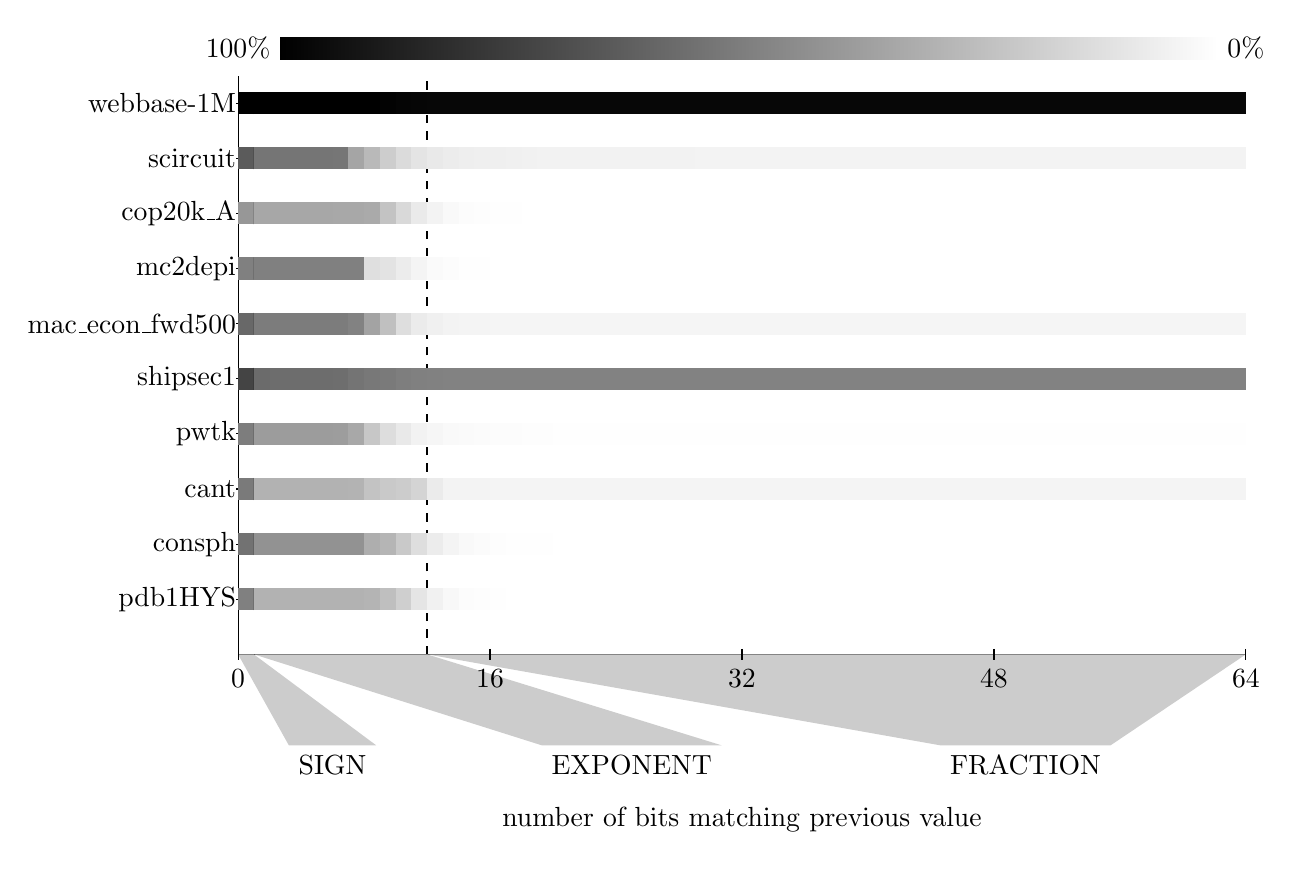
\begin{tikzpicture}[xscale=.2, yscale=.7]
\path[draw] (0,0) -- (64,0);
\path[draw] (0,0) -- (0, 10.5);
\path[draw,dashed] (12,0) -- (12,10.5);
\node(sign) at (6,-2){SIGN};
\node(expo) at (25,-2){EXPONENT};
\node(frac) at (50,-2){FRACTION};
\path[fill=black!20](0,0) -- (1,0) -- (sign.north east) -- (sign.north west) -- cycle;
\path[fill=black!20](1,0) -- (12,0) -- (expo.north east) -- (expo.north west) -- cycle;
\path[fill=black!20](12,0) -- (64,0) -- (frac.north east) -- (frac.north west) -- cycle;

\node[fill=white] at (0,11)(high){100\%};
\node[fill=white] at (64,11)(low){0\%};
\shade[left color=black,right color=white] ([yshift=-.2cm]high.east) rectangle ([yshift=.2cm]low.west);
\foreach \x in {0,16,32,48,64}{
    \draw (\x,.1) -- (\x,-.1)node[anchor=north]{\x};
}

\foreach \n/\y in {pdb1HYS/1, consph/2, cant/3, pwtk/4, shipsec1/5, mac\_econ\_fwd500/6, mc2depi/7, cop20k\_A/8, scircuit/9, webbase-1M/10}{
    \draw (.1,\y) -- (-.1,\y)node[anchor=east,rotate=0,inner sep=0]{\n};
}
\node at (32,-3) {number of bits matching previous value};

    %\shade[left color=black!\ya, right color=black!\yb] (\xa,0.8) rectangle (\xb,1.2);
    %\fill[color=black!\yb] (\xa,0.8) rectangle (\xb,1.2);
\foreach \xa/\ya/\xb/\yb in {
0/100.00/1/49.85,1/49.85/2/30.14,2/30.14/3/30.14,3/30.14/4/30.14,4/30.14/5/30.14,5/30.14/6/30.14,6/30.14/7/30.14,7/30.14/8/30.09,8/30.09/9/29.23,9/29.23/10/25.06,10/25.06/11/18.88,11/18.88/12/10.34,12/10.34/13/5.36,13/5.36/14/2.62,14/2.62/15/1.31,15/1.31/16/0.66,16/0.66/17/0.33,17/0.33/18/0.16,18/0.16/19/0.08,19/0.08/20/0.04,20/0.04/21/0.02,21/0.02/22/0.01,22/0.01/23/0.01,23/0.01/24/0.01,24/0.01/25/0.01,25/0.01/26/0.01,26/0.01/27/0.01,27/0.01/28/0.01,28/0.01/29/0.01,29/0.01/30/0.01,30/0.01/31/0.01,31/0.01/32/0.01,32/0.01/33/0.01,33/0.01/34/0.01,34/0.01/35/0.01,35/0.01/36/0.01,36/0.01/37/0.01,37/0.01/38/0.01,38/0.01/39/0.01,39/0.01/40/0.01,40/0.01/41/0.01,41/0.01/42/0.01,42/0.01/43/0.01,43/0.01/44/0.01,44/0.01/45/0.01,45/0.01/46/0.01,46/0.01/47/0.01,47/0.01/48/0.01,48/0.01/49/0.01,49/0.01/50/0.01,50/0.01/51/0.01,51/0.01/52/0.01,52/0.01/53/0.01,53/0.01/54/0.01,54/0.01/55/0.01,55/0.01/56/0.01,56/0.01/57/0.01,57/0.01/58/0.01,58/0.01/59/0.01,59/0.01/60/0.01,60/0.01/61/0.01,61/0.01/62/0.01,62/0.01/63/0.01,63/0.01/64/0.01,}{
    \fill[color=black!\yb] (\xa,0.8) rectangle (\xb,1.2);
}
\foreach \xa/\ya/\xb/\yb in {
0/100.00/1/55.40,1/55.40/2/42.65,2/42.65/3/42.65,3/42.65/4/42.65,4/42.65/5/42.65,5/42.65/6/42.65,6/42.65/7/42.65,7/42.65/8/42.64,8/42.64/9/31.79,9/31.79/10/28.98,10/28.98/11/21.30,11/21.30/12/12.99,12/12.99/13/7.55,13/7.55/14/4.33,14/4.33/15/2.49,15/2.49/16/1.43,16/1.43/17/0.83,17/0.83/18/0.51,18/0.51/19/0.33,19/0.33/20/0.24,20/0.24/21/0.19,21/0.19/22/0.16,22/0.16/23/0.15,23/0.15/24/0.14,24/0.14/25/0.14,25/0.14/26/0.14,26/0.14/27/0.14,27/0.14/28/0.14,28/0.14/29/0.13,29/0.13/30/0.13,30/0.13/31/0.13,31/0.13/32/0.13,32/0.13/33/0.13,33/0.13/34/0.13,34/0.13/35/0.13,35/0.13/36/0.13,36/0.13/37/0.13,37/0.13/38/0.13,38/0.13/39/0.13,39/0.13/40/0.13,40/0.13/41/0.13,41/0.13/42/0.13,42/0.13/43/0.13,43/0.13/44/0.13,44/0.13/45/0.13,45/0.13/46/0.13,46/0.13/47/0.13,47/0.13/48/0.13,48/0.13/49/0.13,49/0.13/50/0.13,50/0.13/51/0.13,51/0.13/52/0.13,52/0.13/53/0.13,53/0.13/54/0.13,54/0.13/55/0.13,55/0.13/56/0.13,56/0.13/57/0.13,57/0.13/58/0.13,58/0.13/59/0.13,59/0.13/60/0.13,60/0.13/61/0.13,61/0.13/62/0.13,62/0.13/63/0.13,63/0.13/64/0.13,}{
    \fill[color=black!\yb] (\xa,1.8) rectangle (\xb,2.2);
}
\foreach \xa/\ya/\xb/\yb in {
0/100.00/1/52.33,1/52.33/2/30.36,2/30.36/3/30.36,3/30.36/4/30.36,4/30.36/5/30.36,5/30.36/6/30.36,6/30.36/7/30.13,7/30.13/8/29.96,8/29.96/9/23.37,9/23.37/10/21.31,10/21.31/11/19.95,11/19.95/12/17.04,12/17.04/13/7.94,13/7.94/14/4.56,14/4.56/15/4.56,15/4.56/16/4.53,16/4.53/17/4.37,17/4.37/18/4.36,18/4.36/19/4.36,19/4.36/20/4.35,20/4.35/21/4.35,21/4.35/22/4.35,22/4.35/23/4.35,23/4.35/24/4.35,24/4.35/25/4.35,25/4.35/26/4.35,26/4.35/27/4.35,27/4.35/28/4.35,28/4.35/29/4.35,29/4.35/30/4.35,30/4.35/31/4.35,31/4.35/32/4.35,32/4.35/33/4.35,33/4.35/34/4.35,34/4.35/35/4.35,35/4.35/36/4.35,36/4.35/37/4.35,37/4.35/38/4.35,38/4.35/39/4.35,39/4.35/40/4.35,40/4.35/41/4.35,41/4.35/42/4.35,42/4.35/43/4.35,43/4.35/44/4.35,44/4.35/45/4.35,45/4.35/46/4.35,46/4.35/47/4.35,47/4.35/48/4.35,48/4.35/49/4.35,49/4.35/50/4.35,50/4.35/51/4.35,51/4.35/52/4.35,52/4.35/53/4.35,53/4.35/54/4.35,54/4.35/55/4.35,55/4.35/56/4.35,56/4.35/57/4.35,57/4.35/58/4.35,58/4.35/59/4.35,59/4.35/60/4.35,60/4.35/61/4.35,61/4.35/62/4.35,62/4.35/63/4.35,63/4.35/64/4.35,}{
    \fill[color=black!\yb] (\xa,2.8) rectangle (\xb,3.2);
}
\foreach \xa/\ya/\xb/\yb in {
0/100.00/1/50.92,1/50.92/2/38.78,2/38.78/3/38.68,3/38.68/4/38.68,4/38.68/5/38.68,5/38.68/6/38.68,6/38.68/7/38.62,7/38.62/8/33.96,8/33.96/9/22.15,9/22.15/10/13.32,10/13.32/11/8.67,11/8.67/12/5.24,12/5.24/13/3.42,13/3.42/14/2.37,14/2.37/15/1.87,15/1.87/16/1.55,16/1.55/17/1.33,17/1.33/18/1.06,18/1.06/19/0.80,19/0.80/20/0.63,20/0.63/21/0.49,21/0.49/22/0.44,22/0.44/23/0.43,23/0.43/24/0.42,24/0.42/25/0.41,25/0.41/26/0.41,26/0.41/27/0.41,27/0.41/28/0.41,28/0.41/29/0.41,29/0.41/30/0.41,30/0.41/31/0.41,31/0.41/32/0.41,32/0.41/33/0.41,33/0.41/34/0.41,34/0.41/35/0.41,35/0.41/36/0.41,36/0.41/37/0.41,37/0.41/38/0.41,38/0.41/39/0.41,39/0.41/40/0.41,40/0.41/41/0.41,41/0.41/42/0.41,42/0.41/43/0.41,43/0.41/44/0.41,44/0.41/45/0.41,45/0.41/46/0.41,46/0.41/47/0.41,47/0.41/48/0.41,48/0.41/49/0.41,49/0.41/50/0.41,50/0.41/51/0.41,51/0.41/52/0.41,52/0.41/53/0.41,53/0.41/54/0.41,54/0.41/55/0.41,55/0.41/56/0.41,56/0.41/57/0.41,57/0.41/58/0.41,58/0.41/59/0.41,59/0.41/60/0.41,60/0.41/61/0.41,61/0.41/62/0.41,62/0.41/63/0.41,63/0.41/64/0.41,}{
    \fill[color=black!\yb] (\xa,3.8) rectangle (\xb,4.2);
}
\foreach \xa/\ya/\xb/\yb in {
0/100.00/1/73.19,1/73.19/2/58.16,2/58.16/3/57.23,3/57.23/4/57.23,4/57.23/5/57.23,5/57.23/6/57.23,6/57.23/7/56.76,7/56.76/8/54.57,8/54.57/9/52.94,9/52.94/10/52.02,10/52.02/11/50.78,11/50.78/12/49.92,12/49.92/13/49.38,13/49.38/14/49.14,14/49.14/15/49.03,15/49.03/16/48.99,16/48.99/17/48.98,17/48.98/18/48.96,18/48.96/19/48.96,19/48.96/20/48.96,20/48.96/21/48.96,21/48.96/22/48.95,22/48.95/23/48.95,23/48.95/24/48.95,24/48.95/25/48.95,25/48.95/26/48.95,26/48.95/27/48.95,27/48.95/28/48.95,28/48.95/29/48.95,29/48.95/30/48.95,30/48.95/31/48.95,31/48.95/32/48.95,32/48.95/33/48.95,33/48.95/34/48.95,34/48.95/35/48.95,35/48.95/36/48.95,36/48.95/37/48.95,37/48.95/38/48.95,38/48.95/39/48.95,39/48.95/40/48.95,40/48.95/41/48.95,41/48.95/42/48.95,42/48.95/43/48.95,43/48.95/44/48.95,44/48.95/45/48.95,45/48.95/46/48.95,46/48.95/47/48.95,47/48.95/48/48.95,48/48.95/49/48.95,49/48.95/50/48.95,50/48.95/51/48.95,51/48.95/52/48.95,52/48.95/53/48.95,53/48.95/54/48.95,54/48.95/55/48.95,55/48.95/56/48.95,56/48.95/57/48.95,57/48.95/58/48.95,58/48.95/59/48.95,59/48.95/60/48.95,60/48.95/61/48.95,61/48.95/62/48.95,62/48.95/63/48.95,63/48.95/64/48.95,}{
    \fill[color=black!\yb] (\xa,4.8) rectangle (\xb,5.2);
}
\foreach \xa/\ya/\xb/\yb in {
0/100.00/1/59.09,1/59.09/2/51.55,2/51.55/3/51.55,3/51.55/4/51.55,4/51.55/5/51.55,5/51.55/6/51.55,6/51.55/7/51.55,7/51.55/8/48.90,8/48.90/9/35.89,9/35.89/10/24.78,10/24.78/11/12.76,11/12.76/12/7.66,12/7.66/13/5.82,13/5.82/14/4.89,14/4.89/15/4.46,15/4.46/16/4.21,16/4.21/17/4.07,17/4.07/18/3.87,18/3.87/19/3.79,19/3.79/20/3.78,20/3.78/21/3.78,21/3.78/22/3.77,22/3.77/23/3.77,23/3.77/24/3.77,24/3.77/25/3.77,25/3.77/26/3.77,26/3.77/27/3.77,27/3.77/28/3.77,28/3.77/29/3.77,29/3.77/30/3.77,30/3.77/31/3.74,31/3.74/32/3.73,32/3.73/33/3.73,33/3.73/34/3.73,34/3.73/35/3.73,35/3.73/36/3.73,36/3.73/37/3.73,37/3.73/38/3.73,38/3.73/39/3.73,39/3.73/40/3.73,40/3.73/41/3.73,41/3.73/42/3.73,42/3.73/43/3.73,43/3.73/44/3.73,44/3.73/45/3.73,45/3.73/46/3.73,46/3.73/47/3.73,47/3.73/48/3.73,48/3.73/49/3.73,49/3.73/50/3.73,50/3.73/51/3.73,51/3.73/52/3.73,52/3.73/53/3.73,53/3.73/54/3.73,54/3.73/55/3.73,55/3.73/56/3.73,56/3.73/57/3.73,57/3.73/58/3.73,58/3.73/59/3.73,59/3.73/60/3.73,60/3.73/61/3.73,61/3.73/62/3.73,62/3.73/63/3.73,63/3.73/64/3.73,}{
    \fill[color=black!\yb] (\xa,5.8) rectangle (\xb,6.2);
}
\foreach \xa/\ya/\xb/\yb in {
0/100.00/1/49.93,1/49.93/2/49.85,2/49.85/3/49.85,3/49.85/4/49.85,4/49.85/5/49.85,5/49.85/6/49.85,6/49.85/7/49.85,7/49.85/8/49.85,8/49.85/9/12.48,9/12.48/10/11.11,10/11.11/11/7.59,11/7.59/12/4.18,12/4.18/13/2.09,13/2.09/14/1.05,14/1.05/15/0.52,15/0.52/16/0.26,16/0.26/17/0.13,17/0.13/18/0.07,18/0.07/19/0.04,19/0.04/20/0.02,20/0.02/21/0.02,21/0.02/22/0.02,22/0.02/23/0.02,23/0.02/24/0.02,24/0.02/25/0.02,25/0.02/26/0.02,26/0.02/27/0.02,27/0.02/28/0.02,28/0.02/29/0.02,29/0.02/30/0.02,30/0.02/31/0.02,31/0.02/32/0.02,32/0.02/33/0.02,33/0.02/34/0.02,34/0.02/35/0.02,35/0.02/36/0.02,36/0.02/37/0.02,37/0.02/38/0.02,38/0.02/39/0.02,39/0.02/40/0.02,40/0.02/41/0.02,41/0.02/42/0.02,42/0.02/43/0.02,43/0.02/44/0.02,44/0.02/45/0.02,45/0.02/46/0.02,46/0.02/47/0.02,47/0.02/48/0.02,48/0.02/49/0.02,49/0.02/50/0.02,50/0.02/51/0.02,51/0.02/52/0.02,52/0.02/53/0.02,53/0.02/54/0.02,54/0.02/55/0.02,55/0.02/56/0.02,56/0.02/57/0.02,57/0.02/58/0.02,58/0.02/59/0.02,59/0.02/60/0.02,60/0.02/61/0.02,61/0.02/62/0.02,62/0.02/63/0.02,63/0.02/64/0.02,}{
    \fill[color=black!\yb] (\xa,6.8) rectangle (\xb,7.2);
}
\foreach \xa/\ya/\xb/\yb in {
0/100.00/1/40.96,1/40.96/2/34.32,2/34.32/3/34.32,3/34.32/4/34.32,4/34.32/5/34.32,5/34.32/6/34.32,6/34.32/7/34.29,7/34.29/8/34.27,8/34.27/9/33.30,9/33.30/10/23.61,10/23.61/11/14.84,11/14.84/12/8.33,12/8.33/13/4.60,13/4.60/14/2.43,14/2.43/15/1.29,15/1.29/16/0.70,16/0.70/17/0.40,17/0.40/18/0.24,18/0.24/19/0.15,19/0.15/20/0.10,20/0.10/21/0.06,21/0.06/22/0.04,22/0.04/23/0.04,23/0.04/24/0.03,24/0.03/25/0.03,25/0.03/26/0.03,26/0.03/27/0.03,27/0.03/28/0.03,28/0.03/29/0.03,29/0.03/30/0.03,30/0.03/31/0.02,31/0.02/32/0.02,32/0.02/33/0.02,33/0.02/34/0.02,34/0.02/35/0.02,35/0.02/36/0.02,36/0.02/37/0.02,37/0.02/38/0.02,38/0.02/39/0.02,39/0.02/40/0.02,40/0.02/41/0.02,41/0.02/42/0.02,42/0.02/43/0.02,43/0.02/44/0.02,44/0.02/45/0.02,45/0.02/46/0.02,46/0.02/47/0.02,47/0.02/48/0.02,48/0.02/49/0.02,49/0.02/50/0.02,50/0.02/51/0.02,51/0.02/52/0.02,52/0.02/53/0.02,53/0.02/54/0.02,54/0.02/55/0.02,55/0.02/56/0.02,56/0.02/57/0.02,57/0.02/58/0.02,58/0.02/59/0.02,59/0.02/60/0.02,60/0.02/61/0.02,61/0.02/62/0.02,62/0.02/63/0.02,63/0.02/64/0.02,}{
    \fill[color=black!\yb] (\xa,7.8) rectangle (\xb,8.2);
}
\foreach \xa/\ya/\xb/\yb in {
0/100.00/1/64.34,1/64.34/2/54.22,2/54.22/3/54.22,3/54.22/4/54.22,4/54.22/5/54.22,5/54.22/6/54.22,6/54.22/7/53.67,7/53.67/8/35.26,8/35.26/9/27.48,9/27.48/10/19.55,10/19.55/11/14.08,11/14.08/12/10.56,12/10.56/13/8.73,13/8.73/14/7.60,14/7.60/15/6.81,15/6.81/16/6.44,16/6.44/17/6.11,17/6.11/18/5.91,18/5.91/19/5.51,19/5.51/20/5.29,20/5.29/21/5.24,21/5.24/22/5.09,22/5.09/23/5.07,23/5.07/24/5.04,24/5.04/25/4.99,25/4.99/26/4.97,26/4.97/27/4.93,27/4.93/28/4.92,28/4.92/29/4.91,29/4.91/30/4.90,30/4.90/31/4.90,31/4.90/32/4.90,32/4.90/33/4.90,33/4.90/34/4.90,34/4.90/35/4.89,35/4.89/36/4.89,36/4.89/37/4.88,37/4.88/38/4.87,38/4.87/39/4.87,39/4.87/40/4.87,40/4.87/41/4.87,41/4.87/42/4.87,42/4.87/43/4.87,43/4.87/44/4.87,44/4.87/45/4.87,45/4.87/46/4.87,46/4.87/47/4.87,47/4.87/48/4.87,48/4.87/49/4.87,49/4.87/50/4.87,50/4.87/51/4.87,51/4.87/52/4.87,52/4.87/53/4.87,53/4.87/54/4.87,54/4.87/55/4.87,55/4.87/56/4.87,56/4.87/57/4.87,57/4.87/58/4.87,58/4.87/59/4.87,59/4.87/60/4.87,60/4.87/61/4.87,61/4.87/62/4.87,62/4.87/63/4.87,63/4.87/64/4.87,}{
    \fill[color=black!\yb] (\xa,8.8) rectangle (\xb,9.2);
}
\foreach \xa/\ya/\xb/\yb in {
0/100.00/1/100.00,1/100.00/2/100.00,2/100.00/3/100.00,3/100.00/4/100.00,4/100.00/5/100.00,5/100.00/6/100.00,6/100.00/7/100.00,7/100.00/8/100.00,8/100.00/9/99.93,9/99.93/10/98.70,10/98.70/11/97.98,11/97.98/12/97.60,12/97.60/13/97.44,13/97.44/14/97.30,14/97.30/15/97.22,15/97.22/16/97.18,16/97.18/17/97.16,17/97.16/18/97.16,18/97.16/19/97.16,19/97.16/20/97.16,20/97.16/21/97.16,21/97.16/22/97.16,22/97.16/23/97.16,23/97.16/24/97.16,24/97.16/25/97.16,25/97.16/26/97.16,26/97.16/27/97.16,27/97.16/28/97.16,28/97.16/29/97.16,29/97.16/30/97.16,30/97.16/31/97.16,31/97.16/32/97.16,32/97.16/33/97.16,33/97.16/34/97.16,34/97.16/35/97.16,35/97.16/36/97.16,36/97.16/37/97.16,37/97.16/38/97.16,38/97.16/39/97.16,39/97.16/40/97.16,40/97.16/41/97.16,41/97.16/42/97.16,42/97.16/43/97.16,43/97.16/44/97.16,44/97.16/45/97.16,45/97.16/46/97.16,46/97.16/47/97.16,47/97.16/48/97.16,48/97.16/49/97.16,49/97.16/50/97.16,50/97.16/51/97.16,51/97.16/52/97.16,52/97.16/53/97.16,53/97.16/54/97.16,54/97.16/55/97.16,55/97.16/56/97.16,56/97.16/57/97.16,57/97.16/58/97.16,58/97.16/59/97.16,59/97.16/60/97.16,60/97.16/61/97.16,61/97.16/62/97.16,62/97.16/63/97.16,63/97.16/64/97.16,}{
    \fill[color=black!\yb] (\xa,9.8) rectangle (\xb,10.2);
}

\end{tikzpicture}
\caption[Floating point prefix analysis.]{The above figure represents local prefix prediction. The figure shows the density function of 2 adjacent values sharing at least $x$ number of prefix bits. All of the data sets start at $(0,100\%)$. The curves end at the percent of values that are identical to their previous value for that dataset.}
\label{fig:prefix}
\end{figure}%
Datasets might also have repeating patterns of values. For example, the sequence $1.0$, $2.0$, $3.0$, $1.0$, $2.0$, $3.0$ has an obvious pattern. One can use the Burrows Wheeler Transform\cite{prelim:burrows} to analyze these patterns. \figurename~\ref{fig:bwt} describes this algorithm some, however, many other sources describe this algorithm in more detail, for example \cite{prelim:burrows,prelim:salomon}. \figurename~\ref{fig:pattern} analyzes the number of repeats that appear after the Burrow-Wheeler Transform. As the figure shows, BWT reveals patterns in about half of the matrices, but these are also the matrices with a lot of repeats to begin with.
\begin{figure}
\center
\begin{subfigure}{.3\linewidth}
\footnotesize
\textcolor{gray}{
\textcolor{black}{ABCDEABCDEABC\$}\\
\$ABCDEABCDEABC\\
C\$ABCDEABCDEAB\\
BC\$ABCDEABCDEA\\
ABC\$ABCDEABCDE\\
EABC\$ABCDEABCD\\
DEABC\$ABCDEABC\\
CDEABC\$ABCDEAB\\
BCDEABC\$ABCDEA\\
ABCDEABC\$ABCDE\\
EABCDEABC\$ABCD\\
DEABCDEABC\$ABC\\
CDEABCDEABC\$AB\\
BCDEABCDEABC\$A\\
}
\caption{Step1: Generate every cyclic rotation of the original sequence (the first row).}
\label{fig:bwtStep1}
\end{subfigure}
\begin{subfigure}{.3\linewidth}
\footnotesize
\textcolor{gray}{
ABCDEABCDEABC\textcolor{black}{\$}\\
ABCDEABC\$ABCD\textcolor{black}{E}\\
ABC\$ABCDEABCD\textcolor{black}{E}\\
BCDEABCDEABC\$\textcolor{black}{A}\\
BCDEABC\$ABCDE\textcolor{black}{A}\\
BC\$ABCDEABCDE\textcolor{black}{A}\\
CDEABCDEABC\$A\textcolor{black}{B}\\
CDEABC\$ABCDEA\textcolor{black}{B}\\
C\$ABCDEABCDEA\textcolor{black}{B}\\
DEABCDEABC\$AB\textcolor{black}{C}\\
DEABC\$ABCDEAB\textcolor{black}{C}\\
EABCDEABC\$ABC\textcolor{black}{D}\\
EABC\$ABCDEABC\textcolor{black}{D}\\
\$ABCDEABCDEAB\textcolor{black}{C}\\
}
\caption{Step2: Sort the rotations. Then the last element in each new row creates the transformed sequence.}
\label{fig:bwtStep2}
\end{subfigure}
\begin{subfigure}{.3\linewidth}
\footnotesize
\textcolor{gray}{\textcolor{black}{\$E}E\textcolor{black}{A}AA\textcolor{black}{B}BB\textcolor{black}{C}C\textcolor{black}{D}D\textcolor{black}{C}}\\
\caption{Step3: This transformed sequence often has consecutive repeats. (This example does.)}
\label{fig:bwtStep3}
\end{subfigure}
\caption[Burrows Wheeler Transform]{Above shows the Burrows-Wheeler Transform and subsequent compression. Steps 1 and 2 show the brute force calculation of BWT.}
\label{fig:bwt}
\end{figure}
\begin{figure}
\center
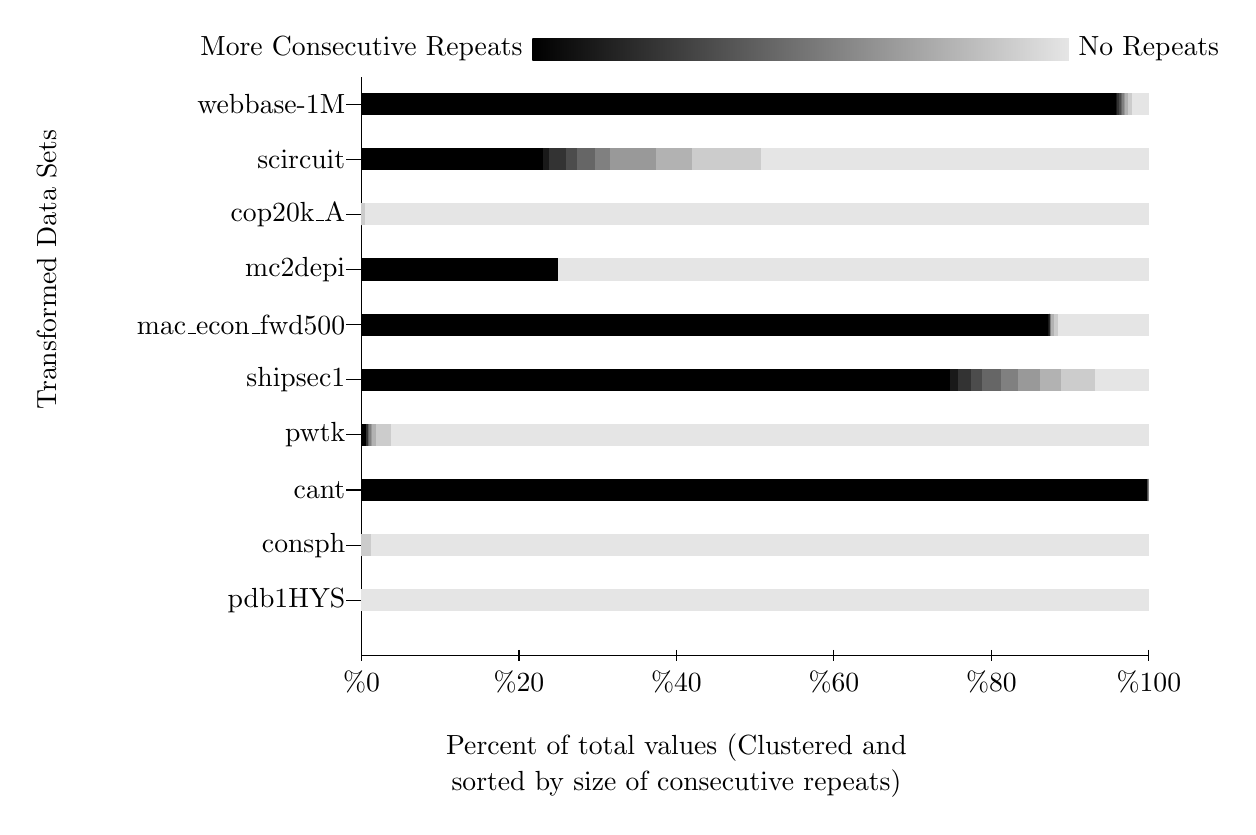
\begin{tikzpicture}[yscale=.7,xscale=2]
\path[draw] (0,0) -- (0,10.5);
\path[draw] (0,0) -- (5,0);
\foreach \x/\v in {0/0,1/20,2/40,3/60,4/80,5/100}{
    \draw (\x,.1) -- (\x,-.1)node[anchor=north]{\%\v};
}
\node[fill=white] at (0,11)(high){More Consecutive Repeats};
\node[fill=white] at (5,11)(low){No Repeats};
\shade[left color=black,right color=black!10] ([yshift=-.2cm]high.east) rectangle ([yshift=.2cm]low.west);

\foreach \n/\y in {pdb1HYS/1, consph/2, cant/3, pwtk/4, shipsec1/5, mac\_econ\_fwd500/6, mc2depi/7, cop20k\_A/8, scircuit/9, webbase-1M/10}{
    \draw (.1,\y) -- (-.1,\y)node[anchor=east,rotate=0,inner sep=0]{\n};
}
\node at (2,-2){\shortstack{Percent of total values (Clustered and \\sorted by size of consecutive repeats)}};
\node[rotate=90] at (-2,7){Transformed Data Sets};

\foreach \s/\xa/\xb in {
100/0.00/0.00,90/0.00/0.00,80/0.00/0.00,70/0.00/0.00,60/0.00/0.00,50/0.00/0.00,40/0.00/0.00,30/0.00/0.00,20/0.00/0.00,10/0.00/5.00}{
    \fill[black!\s] (\xa,0.8) rectangle (\xb,1.2);
}
\foreach \s/\xa/\xb in {
100/0.00/0.00,90/0.00/0.00,80/0.00/0.00,70/0.00/0.00,60/0.00/0.00,50/0.00/0.00,40/0.00/0.00,30/0.00/0.00,20/0.00/0.06,10/0.06/5.00}{
    \fill[black!\s] (\xa,1.8) rectangle (\xb,2.2);
}
\foreach \s/\xa/\xb in {
100/0.00/4.99,90/4.99/4.99,80/4.99/4.99,70/4.99/5.00,60/5.00/5.00,50/5.00/5.00,40/5.00/5.00,30/5.00/5.00,20/5.00/5.00,10/5.00/5.00}{
    \fill[black!\s] (\xa,2.8) rectangle (\xb,3.2);
}
\foreach \s/\xa/\xb in {
100/0.00/0.03,90/0.03/0.03,80/0.03/0.04,70/0.04/0.04,60/0.04/0.05,50/0.05/0.06,40/0.06/0.07,30/0.07/0.09,20/0.09/0.19,10/0.19/5.00}{
    \fill[black!\s] (\xa,3.8) rectangle (\xb,4.2);
}
\foreach \s/\xa/\xb in {
100/0.00/3.74,90/3.74/3.79,80/3.79/3.87,70/3.87/3.94,60/3.94/4.06,50/4.06/4.17,40/4.17/4.31,30/4.31/4.44,20/4.44/4.66,10/4.66/5.00}{
    \fill[black!\s] (\xa,4.8) rectangle (\xb,5.2);
}
\foreach \s/\xa/\xb in {
100/0.00/4.36,90/4.36/4.37,80/4.37/4.37,70/4.37/4.37,60/4.37/4.37,50/4.37/4.38,40/4.38/4.38,30/4.38/4.40,20/4.40/4.42,10/4.42/5.00}{
    \fill[black!\s] (\xa,5.8) rectangle (\xb,6.2);
}
\foreach \s/\xa/\xb in {
100/0.00/1.25,90/1.25/1.25,80/1.25/1.25,70/1.25/1.25,60/1.25/1.25,50/1.25/1.25,40/1.25/1.25,30/1.25/1.25,20/1.25/1.25,10/1.25/5.00}{
    \fill[black!\s] (\xa,6.8) rectangle (\xb,7.2);
}
\foreach \s/\xa/\xb in {
100/0.00/0.00,90/0.00/0.00,80/0.00/0.00,70/0.00/0.00,60/0.00/0.00,50/0.00/0.00,40/0.00/0.00,30/0.00/0.00,20/0.00/0.02,10/0.02/5.00}{
    \fill[black!\s] (\xa,7.8) rectangle (\xb,8.2);
}
\foreach \s/\xa/\xb in {
100/0.00/1.15,90/1.15/1.19,80/1.19/1.30,70/1.30/1.37,60/1.37/1.48,50/1.48/1.58,40/1.58/1.87,30/1.87/2.10,20/2.10/2.54,10/2.54/5.00}{
    \fill[black!\s] (\xa,8.8) rectangle (\xb,9.2);
}
\foreach \s/\xa/\xb in {
100/0.00/4.79,90/4.79/4.80,80/4.80/4.81,70/4.81/4.82,60/4.82/4.83,50/4.83/4.84,40/4.84/4.85,30/4.85/4.87,20/4.87/4.89,10/4.89/5.00}{
    \fill[black!\s] (\xa,9.8) rectangle (\xb,10.2);
}

%TODO: key
\small
%\node at (2,14) {\shortstack{Percent of values in repeating sequences of length $\geq10$ \tikz \draw[fill=green] (0,0) rectangle (.25,.25);,\\ between $10$ and $1$ \tikz \draw[fill=yellow] (0,0) rectangle (.25,.25);, $=1$ \tikz \draw[fill=red] (0,0) rectangle (.25,.25);}};
\end{tikzpicture}
\caption[Floating point pattern analysis using BWT.]{Pattern analysis using the Burrows-Wheeler Transform. Each shade represents the number of consecutive repeats in a repeating sequence. \tikz{\fill[black] (0,0) rectangle (.25,.25);} represents sequences longer than 9. \tikz \fill[black!50] (0,0) rectangle (.25,.25); represents sequences of length 5. \tikz \fill[black!10] (0,0) rectangle (.25,.25); represents sequences equal to 1 (non-repeating).}
\label{fig:pattern}
\end{figure}

\section{Our Approach}
\label{sec:fzipapproach}
Since BWT does not provide great compression, depends on the traversal of the matrix and is not hardware amenable, we designed fzip to only use prefix and repeat compression.
\begin{figure}
\center
\begin{subfigure}{\linewidth}
\center
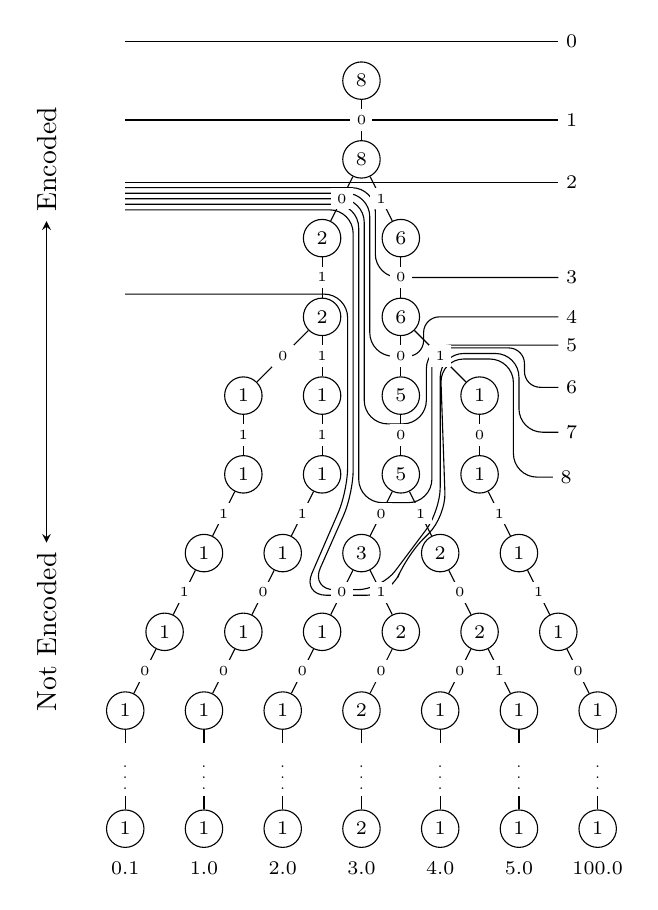
\begin{tikzpicture}
\scriptsize
\node[draw,circle] at (0,0)(n00){8};
%level1
\node[draw,circle] at (0,-1)(n10){8};
%level2
\node[draw,circle] at (-.5,-2)(n20){2};
\node[draw,circle] at (.5,-2)(n21){6};
\node[draw,circle] at (-.5,-3)(n30){2};
\node[draw,circle] at (.5,-3)(n31){6};

\node[draw,circle] at (-1.5,-4)(n40){1};
\node[draw,circle] at (-.5,-4)(n41){1};
\node[draw,circle] at (.5,-4)(n42){5};
\node[draw,circle] at (1.5,-4)(n43){1};

\node[draw,circle] at (-1.5,-5)(n50){1};
\node[draw,circle] at (-.5,-5)(n51){1};
\node[draw,circle] at (.5,-5)(n52){5};
\node[draw,circle] at (1.5,-5)(n53){1};

\node[draw,circle] at (-2,-6)(n60){1};
\node[draw,circle] at (-1,-6)(n61){1};
\node[draw,circle] at (0,-6)(n62){3};
\node[draw,circle] at (1,-6)(n63){2};
\node[draw,circle] at (2,-6)(n64){1};

\node[draw,circle] at (-2.5,-7)(n70){1};
\node[draw,circle] at (-1.5,-7)(n71){1};
\node[draw,circle] at (-0.5,-7)(n72){1};
\node[draw,circle] at (0.5,-7)(n73){2};
\node[draw,circle] at (1.5,-7)(n74){2};
\node[draw,circle] at (2.5,-7)(n75){1};

\node[draw,circle] at (-3,-8)(n80){1};
\node[draw,circle] at (-2,-8)(n81){1};
\node[draw,circle] at (-1, -8)(n82){1};
\node[draw,circle] at (0, -8)(n83){2};
\node[draw,circle] at (1, -8)(n84){1};
\node[draw,circle] at (2, -8)(n85){1};
\node[draw,circle] at (3, -8)(n86){1};

\node[draw,circle] at (-3,-9.5)(n90){1};
\node[draw,circle] at (-2,-9.5)(n91){1};
\node[draw,circle] at (-1,-9.5)(n92){1};
\node[draw,circle] at (0,-9.5)(n93){2};
\node[draw,circle] at (1,-9.5)(n94){1};
\node[draw,circle] at (2,-9.5)(n95){1};
\node[draw,circle] at (3,-9.5)(n96){1};
\scriptsize
\node at (-3,-10){0.1};
\node at (-2,-10){1.0};
\node at (-1,-10){2.0};
\node at (0,-10){3.0};
\node at (1,-10){4.0};
\node at (2,-10){5.0};
\node at (3,-10){100.0};

\scriptsize
\path[draw] (-3,.5) -- (2.5,.5)[anchor=west]node{0};
\path[draw] (-3,-.5) -- (2.5,-.5)[anchor=west]node{1};
\path[draw,yshift=6] (-3,-1.5) -- (2.5,-1.5)[anchor=west]node{2};
%\path[draw,rounded corners=.3cm,yshift=.2cm] (-2.5, -1.5) [shift={(.2cm,.2cm)}] -- (0, -1.5) -- (0,-2.5) -- (2,-2.5);
\path[draw,rounded corners=.3cm,yshift=4] (-3, -1.5) [xshift=5]-- (0, -1.5) [yshift=-4]-- (0,-2.5) [xshift=-5]-- (2.5,-2.5)node[anchor=west]{3};
\path[draw,rounded corners=.3cm,yshift=2] (-3, -1.5) [xshift=3]-- (0, -1.5) [yshift=-2]-- (0,-3.5) [xshift=-9,rounded corners=.2cm] -- (1,-3.5) -- (1,-3) [xshift=6]-- (2.5,-3)node[anchor=west]{4};

\path[draw,rounded corners=.3cm,yshift=0] (-3, -1.5) [xshift=1]-- (0, -1.5) [yshift=4]-- (0,-4.5) [xshift=-6]-- (1,-4.5) -- (1,-3.5) [xshift=5]-- (2.5,-3.5)node[anchor=west]{5};
\path[draw,rounded corners=.3cm,yshift=-2] (-3, -1.5) [xshift=-1]-- (0, -1.5) [yshift=6]-- (0,-5.5) [xshift=-2]-- (1,-5.5) [rounded corners=.2cm,yshift=-1]-- (1,-3.5) [xshift=5]-- (2,-3.5) -- (2,-4) [xshift=-2]-- (2.5,-4)node[anchor=west]{6};
\path[draw,rounded corners=.3cm,yshift=-4] (-3, -1.5) [xshift=-3]-- (0, -1.5) [yshift=-3]-- (0,-5) [shift={(6pt,8pt)}]-- (-.75,-6.5) [xshift=-3]-- (.25,-6.5) -- (1,-5.5) -- (1,-3.5) -- (2,-3.5) -- (2,-4.5) -- (2.5,-4.5)node[anchor=west]{7};
\path[draw,rounded corners=.3cm,yshift=-6] (-3, -2.5) [xshift=-5]-- (0, -2.5) -- (0,-5) [shift={(5pt,5pt)}]-- (-.75,-6.5) [xshift=2]-- (.3,-6.5) -- (.5,-6) -- (1,-5.5) [xshift=-2pt]-- (1,-3.5) [xshift=-2]-- (2,-3.5) -- (2,-5) -- (2.5,-5)node[anchor=west]{8};
%\path[draw,rounded corners=.3cm,yshift=-6] (-3, -1.5) [xshift=-5]-- (0, -1.5) -- (0,-5) [shift={(5pt,5pt)}]-- (-.75,-6.5) -- (0,-6.5) [yshift=1]-- (0,-7.5) [rounded corners=.2cm]-- (1,-7.5) [shift={(2pt,-2pt)}]-- (1,-7) -- (.5,-6) -- (.75,-5.5) [xshift=-2pt]-- (1.5,-5.5) -- (1.5,-6) -- (2,-6)node[anchor=west]{8};

%\path[draw] (-2.5,-8.4) .. controls (-2,-8.4) and (-1.7,-8.3) .. (-1.5,-7.9) -- (0,-5) .. controls (.1,-4.8) and (0,-4.5) .. (1,-4.5) -- (2,-4.5)[anchor=west]node{2};
%\path[draw] (-2.5,-8.5) .. controls (-2,-8.5) and (-1.7,-8.4) .. (-1.5,-8.1) -- (-.2,-5.5) .. controls (0,-5.4) .. (.2,-5.5) -- (.5,-6) .. controls (.8,-6.6) and (.8,-6.5) ..(1.5,-6.5) .. controls (2,-6.5) and (1.5,-5.5) .. (2,-5.5)[anchor=west]node{3};
%\path[draw] (-2.5, -8.6) -- (0,-8.6) .. controls (.1,-8.6) and (.2,-8.6) .. (.5,-8) -- (1,-7) .. controls (1.3,-6.5) and (1,-6.6) ..(2,-6.6)node[anchor=west]{4};
%\path[draw] (-2.5, -8.7) -- (2,-8.7)node[anchor=west]{5};
%\path[draw] (
\tiny
\path[draw] (n00) --node[fill=white]{0} (n10);
\path[draw] (n10) --node[fill=white]{0} (n20);
\path[draw] (n10) --node[fill=white]{1} (n21);
\path[draw] (n20) --node[fill=white]{1} (n30);
\path[draw] (n21) --node[fill=white]{0} (n31);
\path[draw] (n30) --node[fill=white]{0} (n40);
\path[draw] (n30) --node[fill=white]{1} (n41);
\path[draw] (n31) --node[fill=white]{0} (n42);
\path[draw] (n31) --node[fill=white]{1} (n43);

\path[draw] (n40) --node[fill=white]{1} (n50);
\path[draw] (n41) --node[fill=white]{1} (n51);
\path[draw] (n42) --node[fill=white]{0} (n52);
\path[draw] (n43) --node[fill=white]{0} (n53);

\path[draw] (n50) --node[fill=white]{1} (n60);
\path[draw] (n51) --node[fill=white]{1} (n61);
\path[draw] (n52) --node[fill=white]{0} (n62);
\path[draw] (n52) --node[fill=white]{1} (n63);
\path[draw] (n53) --node[fill=white]{1} (n64);

\path[draw] (n60) --node[fill=white]{1} (n70);
\path[draw] (n61) --node[fill=white]{0} (n71);
\path[draw] (n62) --node[fill=white]{0} (n72);
\path[draw] (n62) --node[fill=white]{1} (n73);
\path[draw] (n63) --node[fill=white]{0} (n74);
\path[draw] (n64) --node[fill=white]{1} (n75);

\path[draw] (n70) --node[fill=white]{0} (n80);
\path[draw] (n71) --node[fill=white]{0} (n81);
\path[draw] (n72) --node[fill=white]{0} (n82);
\path[draw] (n73) --node[fill=white]{0} (n83);
\path[draw] (n74) --node[fill=white]{0} (n84);
\path[draw] (n74) --node[fill=white]{1} (n85);
\path[draw] (n75) --node[fill=white]{0} (n86);

\path[draw] (n80) --node[fill=white]{$\vdots$} (n90);
\path[draw] (n81) --node[fill=white]{$\vdots$} (n91);
\path[draw] (n82) --node[fill=white]{$\vdots$} (n92);
\path[draw] (n83) --node[fill=white]{$\vdots$} (n93);
\path[draw] (n84) --node[fill=white]{$\vdots$} (n94);
\path[draw] (n85) --node[fill=white]{$\vdots$} (n95);
\path[draw] (n86) --node[fill=white]{$\vdots$} (n96);

\normalsize
\path (-4,-7)node(ne)[rotate=90]{Not Encoded} -- (-4,-1)node(e)[rotate=90,fill=white]{Encoded};
\path[draw,stealth-stealth] (e)--(ne);
\end{tikzpicture}
\caption{Each node in the above tree represents every prefix that occurs in the dataset.}
\label{fig:tree}
\end{subfigure}
\\
\begin{subfigure}{\linewidth}
\center
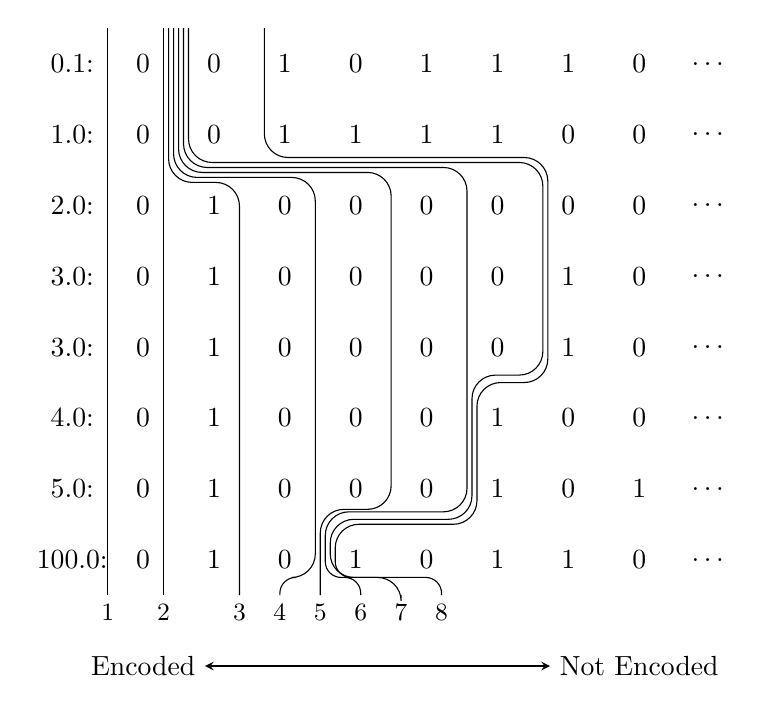
\begin{tikzpicture}[scale=.9]
\node at (0,1){0};\node at (1,1){0};\node at (2,1){1};\node at (3,1){0};\node at (4,1){1};\node at (5,1){1};\node at (6,1){1};\node at (7,1){0};
\node at (0,0){0};\node at (1,0){0};\node at (2,0){1};\node at (3,0){1};\node at (4,0){1};\node at (5,0){1};\node at (6,0){0};\node at (7,0){0};
\node at (0,-1){0};\node at (1,-1){1};\node at (2,-1){0};\node at (3,-1){0};\node at (4,-1){0};\node at (5,-1){0};\node at (6,-1){0};\node at (7,-1){0};
\node at (0,-2){0};\node at (1,-2){1};\node at (2,-2){0};\node at (3,-2){0};\node at (4,-2){0};\node at (5,-2){0};\node at (6,-2){1};\node at (7,-2){0};
\node at (0,-3){0};\node at (1,-3){1};\node at (2,-3){0};\node at (3,-3){0};\node at (4,-3){0};\node at (5,-3){0};\node at (6,-3){1};\node at (7,-3){0};
\node at (0,-4){0};\node at (1,-4){1};\node at (2,-4){0};\node at (3,-4){0};\node at (4,-4){0};\node at (5,-4){1};\node at (6,-4){0};\node at (7,-4){0};
\node at (0,-5){0};\node at (1,-5){1};\node at (2,-5){0};\node at (3,-5){0};\node at (4,-5){0};\node at (5,-5){1};\node at (6,-5){0};\node at (7,-5){1};
\node at (0,-6){0};\node at (1,-6){1};\node at (2,-6){0};\node at (3,-6){1};\node at (4,-6){0};\node at (5,-6){1};\node at (6,-6){1};\node at (7,-6){0};

\node at (8,1){\dots};
\node at (8,0){\dots};
\node at (8,-1){\dots};
\node at (8,-2){\dots};
\node at (8,-3){\dots};
\node at (8,-4){\dots};
\node at (8,-5){\dots};
\node at (8,-6){\dots};

\node at (-1,1){0.1:};\node at (-1,0){1.0:};\node at (-1,-1){2.0:};\node at (-1,-2){3.0:};\node at (-1,-3){3.0:};\node at (-1,-4){4.0:};\node at (-1,-5){5.0:};\node at (-1,-6){100.0:};

\small

\path[draw] (-.5,1.5) -- (-.5,-6.5)node[anchor=north]{1};
\path[draw,xshift=-6] (.5,1.5) -- (.5,-6.5)node[anchor=north]{2};
\path[draw,rounded corners=.3cm,xshift=-4] (.5,1.5) [yshift=-5]-- (.5,-.5) -- (1.5,-.5) [yshift=5]-- (1.5,-6.5)node[anchor=north]{3};
\path[draw,rounded corners=.3cm,xshift=-2] (.5,1.5) [yshift=-3]-- (.5,-.5) -- (2.5,-.5) [yshift=3]-- (2.5,-6.25) [rounded corners=.2cm]-- (2,-6.25) -- (2,-6.5)node[anchor=north]{4};
\path[draw,rounded corners=.3cm,xshift=0] (.5,1.5) [yshift=-1]-- (.5,-.5) -- (3.5,-.5) [yshift=7]-- (3.5,-5.5) -- (2.5,-5.5) [yshift=-6]-- (2.5,-6.5)node[anchor=north]{5};
\path[draw,rounded corners=.3cm,xshift=2] (.5,1.5) [yshift=1]-- (.5,-.5) -- (4.5,-.5) [yshift=4]-- (4.5,-5.5) -- (2.5,-5.5)[rounded corners=.2cm,yshift=-5]-- (2.5,-6.25) -- (3,-6.25) -- (3,-6.5)node[anchor=north]{6};
\path[draw,rounded corners=.3cm,xshift=4] (.5,1.5) [yshift=3]-- (.5,-.5) -- (5.5,-.5) -- (5.5, -3.5) -- (4.5,-3.5) [yshift=-1]-- (4.5,-5.5) -- (2.5,-5.5) [yshift=-2]-- (2.5,-6.25) -- (3.5,-6.25) -- (3.5,-6.5)node[anchor=north]{7};
\path[draw,rounded corners=.3cm,xshift=6] (1.5,1.5) [yshift=5]-- (1.5,-.5) -- (5.5,-.5) [yshift=-5]-- (5.5,-1.5) -- (5.5,-3.5) -- (4.5,-3.5) -- (4.5,-5.5) -- (2.5,-5.5)[rounded corners=.2cm]-- (2.5,-6.25) -- (4,-6.25) -- (4,-6.5)node[anchor=north]{8};
%\path[draw,rounded corners=.3cm,xshift=6] (.5,1.5) [yshift=5]-- (.5,-.5) -- (5.5,-.5) [yshift=-5]-- (5.5,-1.5) -- (6.5,-1.5) -- (6.5, -3.5) -- (4.5,-3.5) [rounded corners=.2cm]-- (4.5,-5.25) -- (5,-5.25) -- (5,-5.5)node[anchor=north]{8};
\normalsize
\path (0,-7.5)node(e){Encoded} -- (7,-7.5)node(ne){Not Encoded};
\path[draw,stealth-stealth] (e)--(ne);
\end{tikzpicture}
\caption{The above sorted list of values gives a second visual representation of how the partition grows.}
\end{subfigure}
\caption[The floating point prefix compression algorithm.]{The above 2 figures show the first 8 partition cuts for prefix compression for the example dataset \{0.1, 1.0, 3.0, 5.0, 3.0, 100.0, 4.0, 2.0\}. For simplicity half-precision (16-bit) encoding is used.}
\label{fig:jiles}
\end{figure}
\subsection{Prefix Compression}
fzip uses arithmetic encoding followed by Huffman encoding to encode common prefixes. To begin with, fzip creates a large tree to represent all the values in the array. \figurename~\ref{fig:tree} shows an example tree for a small dataset. The tree follows the following rules: each node has up to two children. Each edge represents a 1 bit or a 0 bit. Each node in the tree represents a prefix. The root node represents ``" or no prefix. Each node also has a weight, which represents the number of values with the prefix the node represents. So, the weight of the root node equals the total number of values. The weight of the left (or 0 bit) child of the root represents the prefix ``0". Its weight represents the number of  values that start with ``0" (all non-negative values). Likewise, the right child of the root represents the prefix ``1" and its weight is the number of values starting with 1 (all the negative values).\par
Several properties appear. First, the sum of all the weights of the nodes in any level equals $nnz$, where $nnz$ is the total number of values. Moreover, the weight of any set of nodes that partitions the root node from the $65^{th}$ level (and does not contain more nodes than necessary to create the partition) equals $nnz$.\par
Second, the tree is unbalanced (in our case this is good). Put another way, the datasets contain an unequal number of positive and negative numbers, also any ``normal" dataset would not have an exponential distribution from $2^{-12}$ to $2^{12}$ in such a way to make the rest of the tree balanced.\par
Tree creation starts with the root node, which has a starting weight of 0. To create the rest of the tree, add each value to the tree in the following way: Create a pointer to a ``current node" $c$ and initiate $c$ to the root node. Increment the weight of $c$ (the root node). Then, with the most significant bit (the sign bit) of the floating point value, update $c$ by following the edge that matches this bit. If this edge does not exist create the edge and corresponding node. Then, increment the weight of the new $c$. This repeats until you reach the $64^{th}$ bit. Then, the next value gets added to the tree. This continues until the last value gets added to the tree.\par
fzip calculates the prefix codes by creating a partition in the tree. To start, fzip creates a partition with only the root node. Then it includes the node with the largest weight that is a child of the partition. This repeats until a predetermined number of edges become cut by the partition. Using a list of prefix, prefix code pairs we can represent the encoding scheme of the first 8 partitions of the example in \figurename~\ref{fig:jiles}:\par
\begin{enumerate}
    \item (0,)
    \item (00,0), (01,1)
    \item (00,0), (010,1)
    \item (00,00), (0100,01), (0101,10)
    \item (00,00), (01000,01), (0101,10)
    \item (00,00), (010000,01), (010001,10), (0101,11)
    \item (00,000), (0100000,001), (0100001,010), (010001,011), (0101,100)
    \item (001,000), (0100000,001), (0100001,010), (010001,011), (0101,100)
\end{enumerate} \par
Each added node improves the compression because of the following observation: Let the last added node equal $A$. The number of bits in the uncompressed (not-encoded) stream decreases by weight($A$). However, the code lengths have to increase because the partition cut-size ($k$) increases. The code lengths equal $\log_2(k)$. So the increase in the code length equals $\log_2(k+1)-\log_2(k)$ or $\frac{1}{k}$ by using derivatives. So the codes stream will increase by $\frac{nnz}{k}$, where $nnz$ equals to number of values in the data set. If you choose $A$ to maximize $\textrm{weight}(A)$ (a greedy algorithm) then $\textrm{weight}(A) > \textrm{average weight of children to the partition} = \frac{nnz}{k}$. Therefore, the total size of the prefix compression, excluding overhead, keeps improving as the partition increases.\\
\indent But, what if a value occurs often? Say the value $1.0$ occurs $10\%$ of the time? Ideally you should encode $1.0$ as 4 bits ($\log_210$ rounded up), but if we continue to grow the partition beyond cutting 16 edges $1.0$ would encode as more than 4 bits. Our solution freezes the codes once a node from the last ($65^{th}$) level becomes included in the partition. This allows fzip to continue to improve prefix compression by growing the partition and also encode common values with shorter codes. This change makes the encoding to variable-length arithmetic encoding.\\
\indent Of course, the overhead to store all of the codes exists. Currently, a 16 byte record describes each code. Each record stores the prefix, the prefix length and the code length. To balance the benefit of prefix encoding with its overhead, we limit the overhead to 256 records.
\subsection{Repeated Value Extension}
Prefix compression does not compress all of the repeated values. So, fzip extends prefix compression to specifically include commonly repeated values. Again explaining why repeated values compress well: All of the datasets have less than 6 million values. An index of 23 bits can address the entire dataset. Even if a value repeats only once (occurs twice) there still exists an advantage to store the repeated values in a repeated value array and store the indexes into this array instead of the original values. In the previous example $23+23+64<64+64$ (2 indices plus the value in the array equals less than storing 2 values).\\
\indent To encode these repeats, we add a special code to the set of prefix codes. We limit the number of repeats to 8192, so when this code is encountered 13 bits will be on the not-encoded stream indicating the address of the common value.

\begin{figure}
\center
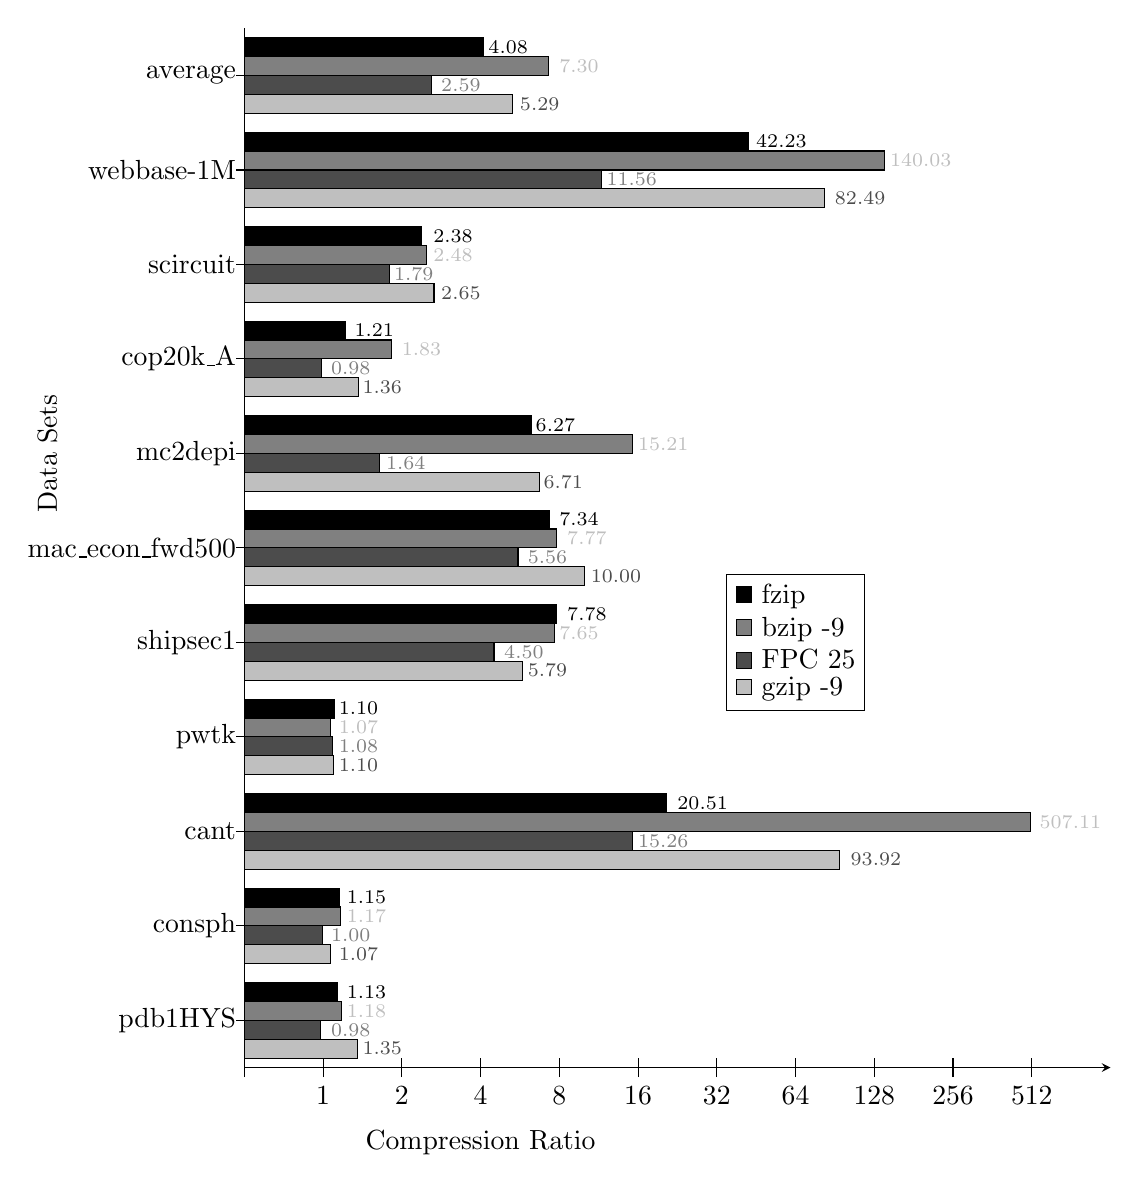
\begin{tikzpicture}[xscale=1,yscale=1.2]
\path[draw] (0,.5) -- (0,11.5);
\path[draw, -stealth] (0,.5) -- (11,.5);
\foreach \x in {0,1,...,10}{
    \path[draw](\x,.4) -- (\x,.6);
}
\foreach \n/\y in {pdb1HYS/1, consph/2, cant/3, pwtk/4, shipsec1/5, mac\_econ\_fwd500/6, mc2depi/7, cop20k\_A/8, scircuit/9, webbase-1M/10, average/11}{
    \draw (.1,\y) -- (-.1,\y)node[anchor=east,rotate=0,inner sep=0]{\n};
}
\foreach \x/\xscale in {1/1,2/2,3/4,4/8,5/16,6/32,7/64,8/128,9/256,10/512}{
    \node[anchor=north] at (\x,.4){\xscale};
}
%labels
\node[rotate = 90] at (-2.5,7){Data Sets};
\node at (3, -.3){Compression Ratio};
%TODO: data
%black!50 black!25 black!70 yellow
%gzip
\foreach \y/\val in
{
    1/1.4381395476381393,2/1.0916733147798856,3/7.553384991365857,4/1.134840892559168,5/3.5325464816899257,6/4.3220742537498005,7/3.7452968046629334,8/1.4474437031978624,9/2.4082861931969743,10/7.3662162703581915,11/3.4039902453198736
}{
    \draw[fill=black!25] (0,\y-.4) rectangle (\val,\y-.2);
}

\foreach \y/\val in {
1/0.9703154387982447,2/0.9940709630537352,3/4.9313813811158385,4/1.1162887682756681,5/3.170250966398405,6/3.475248978449822,7/1.7113132878531525,8/0.9757434397200309,9/1.8431713715699232,10/4.530812321248466,11/2.371859691648329
}{
    \draw[fill=black!70] (0,\y-.2) rectangle (\val,\y);
}


\foreach \y/\val in
{
1/1.2342280655474396,2/1.2260093429943355,3/9.986162958869974,4/1.0951017190297625,5/3.93629964487195,6/3.9586175034412285,7/4.926834410237387,8/1.8710214839874202,9/2.3088144122961687,10/8.12964239568333,11/3.8672731936958997
}{
    \draw[fill=black!50] (0,\y) rectangle (\val,\y+.2);
}

\foreach \y/\val in {
1/1.182412629081373,2/1.204366120271175,3/5.3579179101253285,4/1.1414066312172233,5/3.959223014150452,6/3.8767389203500864,7/3.648371101032564,8/1.2800298418189981,9/2.252300597334877,10/6.4002885786378085,11/3.0303055344019887
}{
    \draw[fill=black] (0,\y+.2) rectangle (\val,\y+.4);
}

\scriptsize
\node[black!50,anchor=west] at (1.0,0.9){0.98};
\node[black,anchor=west] at (1.2,1.3){1.13};
\node[black!25,anchor=west] at (1.2,1.1){1.18};
\node[black!70,anchor=west] at (1.4,0.7){1.35};
\node[black!50,anchor=west] at (1.0,1.9){1.00};
\node[black!70,anchor=west] at (1.1,1.7){1.07};
\node[black,anchor=west] at (1.2,2.3){1.15};
\node[black!25,anchor=west] at (1.2,2.1){1.17};
\node[black!50,anchor=west] at (4.9,2.9){15.26};
\node[black,anchor=west] at (5.4,3.3){20.51};
\node[black!70,anchor=west] at (7.6,2.7){93.92};
\node[black!25,anchor=west] at (10.0,3.1){507.11};
\node[black!25,anchor=west] at (1.1,4.1){1.07};
\node[black!50,anchor=west] at (1.1,3.9){1.08};
\node[black!70,anchor=west] at (1.1,3.7){1.10};
\node[black,anchor=west] at (1.1,4.3){1.10};
\node[black!50,anchor=west] at (3.2,4.9){4.50};
\node[black!70,anchor=west] at (3.5,4.7){5.79};
\node[black!25,anchor=west] at (3.9,5.1){7.65};
\node[black,anchor=west] at (4.0,5.3){7.78};
\node[black!50,anchor=west] at (3.5,5.9){5.56};
\node[black,anchor=west] at (3.9,6.3){7.34};
\node[black!25,anchor=west] at (4.0,6.1){7.77};
\node[black!70,anchor=west] at (4.3,5.7){10.00};
\node[black!50,anchor=west] at (1.7,6.9){1.64};
\node[black,anchor=west] at (3.6,7.3){6.27};
\node[black!70,anchor=west] at (3.7,6.7){6.71};
\node[black!25,anchor=west] at (4.9,7.1){15.21};
\node[black!50,anchor=west] at (1.0,7.9){0.98};
\node[black,anchor=west] at (1.3,8.3){1.21};
\node[black!70,anchor=west] at (1.4,7.7){1.36};
\node[black!25,anchor=west] at (1.9,8.1){1.83};
\node[black!50,anchor=west] at (1.8,8.9){1.79};
\node[black,anchor=west] at (2.3,9.3){2.38};
\node[black!25,anchor=west] at (2.3,9.1){2.48};
\node[black!70,anchor=west] at (2.4,8.7){2.65};
\node[black!50,anchor=west] at (4.5,9.9){11.56};
\node[black,anchor=west] at (6.4,10.3){42.23};
\node[black!70,anchor=west] at (7.4,9.7){82.49};
\node[black!25,anchor=west] at (8.1,10.1){140.03};
\node[black!50,anchor=west] at (2.4,10.9){2.59};
\node[black,anchor=west] at (3.0,11.3){4.08};
\node[black!70,anchor=west] at (3.4,10.7){5.29};
\node[black!25,anchor=west] at (3.9,11.1){7.30};
%\node[black!50,anchor=west] at (1.1,1.1){1.09};
%\node[black,anchor=west] at (1.2,1.3){1.12};
%\node[black!25,anchor=west] at (1.2,0.7){1.13};
%\node[black!70,anchor=west] at (1.4,0.9){1.29};
%\node[black!50,anchor=west] at (1.0,2.1){1.02};
%\node[black!25,anchor=west] at (1.1,1.7){1.05};
%\node[black,anchor=west] at (1.1,2.3){1.08};

\normalsize
\node[draw] at (7,5){\shortstack[l]{
    \tikz \draw[fill=black] (.1,.1) rectangle (.3,.3); fzip\\
    \tikz \draw[fill=black!50] (.1,.1) rectangle (.3,.3); bzip -9\\
    \tikz \draw[fill=black!70] (.1,.1) rectangle (.3,.3); FPC 25\\
    \tikz \draw[fill=black!25] (.1,.1) rectangle (.3,.3); gzip -9
    }};

\end{tikzpicture}
\caption[Floating point compression comparing gzip, bzip, FPC and fzip.]{The comparison of different compression schemes shows fzip performs competitively.}
\label{fig:compare}
\end{figure}
%\begin{figure}
%\center
%\begin{tikzpicture}[xscale=3, yscale=1.2]
%\path[draw, -stealth] (0,.5) -- (3.5,.5);
%\path[draw] (0,.5) -- (0,14.5);
%\foreach \x in {0,1,...,3}{
%    \path[draw](\x,.6) -- (\x,.4);
%}
%\foreach \n/\y in {dense2/1, pdb1HYS/2, consph/3, cant/4, pwtk/5, rma10/6, qcd5\_4/7, shipsec1/8, mac\_econ\_fwd500/9, mc2depi/10, cop20k\_A/11, scircuit/12, webbase-1M/13, average/14}{
%    \draw (.1,\y) -- (-.1,\y)node[anchor=east,rotate=0,inner sep=0]{\n};
%}
%\foreach \x/\yscale in {1/10K,2/100K,3/1M}{ %,4/10M}{
%    \node[anchor=north] at (\x,.4){\yscale};
%}
%
%\node[rotate=90] at (-1.2,5.5) {Data Sets};
%\node at (2,-.3) {Compressed Values per Second};
%
%\foreach \y/\x in {1/3.34,2/3.48,3/3.31,4/3.30,5/3.00,6/2.15,7/2.37,8/3.13,9/2.03,10/3.49,11/3.18}{
%    \draw[rectangle,fill=black!25] (0,\y-.4) rectangle (\x,\y-.2);
%}
%\foreach \y/\x in {1/3.34,2/1.58,3/3.31,4/3.77,5/0.22,6/2.15,7/2.18,8/3.13,9/2.03,10/2.02,11/3.08}{
%    \draw[rectangle,fill=black!70] (0,\y-.2) rectangle (\x,\y);
%}
%\foreach \y/\x in {1/2.86,2/2.88,3/2.46,4/2.99,5/3.60,6/2.50,7/3.32,8/3.13,9/2.98,10/2.71,11/3.08}{
%    \draw[fill=black!50] (0,\y) rectangle (\x,\y+.2);
%}
%\foreach \y/\x in {1/1.55,2/1.58,3/1.83,4/1.41,5/0.22,6/2.15,7/2.18,8/1.75,9/2.03,10/2.02,11/1.86}{
%    \draw[fill=black] (0,\y+.2) rectangle (\x,\y+.4);
%}
%\scriptsize
%\node[black,anchor=west] at (1.5,1.3){35K};
%\node[black!50,anchor=west] at (2.9,1.1){730K};
%\node[black!25,anchor=west] at (3.3,0.7){2.2M};
%\node[black!70,anchor=west] at (3.3,0.9){2.2M};
%\node[black!70,anchor=west] at (1.6,1.9){38K};
%\node[black,anchor=west] at (1.6,2.3){38K};
%\node[black!50,anchor=west] at (2.9,2.1){762K};
%\node[black!25,anchor=west] at (3.5,1.7){3.0M};
%\node[black,anchor=west] at (1.8,3.3){68K};
%\node[black!50,anchor=west] at (2.5,3.1){291K};
%\node[black!25,anchor=west] at (3.3,2.7){2.0M};
%\node[black!70,anchor=west] at (3.3,2.9){2.0M};
%\node[black,anchor=west] at (1.4,4.3){26K};
%\node[black!50,anchor=west] at (3.0,4.1){988K};
%\node[black!25,anchor=west] at (3.3,3.7){2.0M};
%\node[black!70,anchor=west] at (3.8,3.9){5.9M};
%\node[black!70,anchor=west] at (0.2,4.9){2K};
%\node[black,anchor=west] at (0.2,5.3){2K};
%\node[black!25,anchor=west] at (3.0,4.7){994K};
%\node[black!50,anchor=west] at (3.6,5.1){4.0M};
%\node[black!25,anchor=west] at (2.2,5.7){141K};
%\node[black!70,anchor=west] at (2.2,5.9){141K};
%\node[black,anchor=west] at (2.2,6.3){141K};
%\node[black!50,anchor=west] at (2.5,6.1){318K};
%\node[black!70,anchor=west] at (2.2,6.9){150K};
%\node[black,anchor=west] at (2.2,7.3){150K};
%\node[black!25,anchor=west] at (2.4,6.7){233K};
%\node[black!50,anchor=west] at (3.3,7.1){2.1M};
%\node[black,anchor=west] at (1.8,8.3){57K};
%\node[black!25,anchor=west] at (3.1,7.7){1.4M};
%\node[black!70,anchor=west] at (3.1,7.9){1.4M};
%\node[black!50,anchor=west] at (3.1,8.1){1.4M};
%\node[black!25,anchor=west] at (2.0,8.7){107K};
%\node[black!70,anchor=west] at (2.0,8.9){107K};
%\node[black,anchor=west] at (2.0,9.3){107K};
%\node[black!50,anchor=west] at (3.0,9.1){959K};
%\node[black!70,anchor=west] at (2.0,9.9){104K};
%\node[black,anchor=west] at (2.0,10.3){104K};
%\node[black!50,anchor=west] at (2.7,10.1){518K};
%\node[black!25,anchor=west] at (3.5,9.7){3.1M};
%\node[black,anchor=west] at (1.9,11.3){73K};
%\node[black!50,anchor=west] at (3.1,11.1){1.2M};
%\node[black!70,anchor=west] at (3.1,10.9){1.2M};
%\node[black!25,anchor=west] at (3.2,10.7){1.5M};
%\normalsize
%\node[draw,rotate=90] at (-1.2,10){\tikz \draw[fill=black!25] (.1,.1) rectangle (.3,.3); gzip -9 \tikz \draw[fill=black!70] (.1,.1) rectangle (.3,.3); FPC 25 \tikz \draw[fill=black!50] (.1,.1) rectangle (.3,.3); bzip -9 \tikz \draw[fill=black] (.1,.1) rectangle (.3,.3); fzip};
%\end{tikzpicture}
%\caption{The above compression runtime analysis shows that fzip has some improvement to make to compete with other program's runtime.}
%\label{fig:runtime}
%\end{figure}

\section{The fzip decoder}
\label{sec:fzip_decoder}
Like the SMC decoder from Section~\ref{sec:smc_decoder} in the previous chapter, the fzip hardware decoder relies on lookup tables to decode the two streams (see \figurename~\ref{fig:fzip_decoder}). First the dictonary is loaded onto a large 512 value lookup table (LUT). This lookup table uses the code length to determine how much to shift the first shift buffer. The LUT then determines if the second shift buffer is needed (the code is a variable length delta). Then the delta (or newline) is sent to the running row and column index and the current row and column index is outputed from the decoder.
\begin{figure}
    \begin{tikzpicture}
        \node at (0,1) {Memory};
        \node at (4,1) {Decoder};
        \draw [dashed](1.8,1.5) -- (1.8,-5);
        \node at (-.2,0)[draw,trapezium,trapezium right angle=120,trapezium left angle=60](h){Header};
        \node at (-.2,-1)[draw,trapezium,trapezium right angle=120,trapezium left angle=60](d){Dictionary};
        \node at (-.2,-2)[draw,trapezium,trapezium right angle=120,trapezium left angle=60](common){Commons};
        \node at (-.2,-3.2)[draw,trapezium,trapezium right angle=120,trapezium left angle=60](ds){\shortstack{Data\\Stream}};
        \node at (-.2,-4.6)[draw,trapezium,trapezium right angle=120,trapezium left angle=60](as){\shortstack{Argument\\Stream}};

        \node at (5, 0) [draw,minimum width=4cm](sb1){Shifter Buffer};
        \node at (3.5, -1.5) [draw,minimum height=1cm](l){LUT};
        \node at (5, -3) [draw,minimum width=4cm](sb2){Shifter Buffer};

        \node at (9, -4) [minimum width=2cm](shared){\shortstack{Shared\\Memory}};
        \draw (shared.south west) -- (shared.north west) -- (shared.north east) -- (shared.south east);

        \node at (11,-1.5) (output){Output};

        \draw[->,shorten >=2pt] (ds) .. controls ++(1.5,0)  and ++(-2.5,0) .. (sb1);
        \draw[->,shorten >=2pt] (sb1.350) .. controls ++(0,-.5) and ++(0,.5) .. (l.north -| 3.7,0);
        \draw[<-,shorten <=2pt] (sb1.south -| 3.5,0) .. controls ++(0,-.5) and ++(0,.5) .. (l.north -| 3.3,0);
        \draw[->,shorten >=2pt] (as) .. controls ++(1.5,0) and ++(-2.5,0) .. (sb2);
        \draw[->,shorten >=2pt] (l) -- (l|-sb2.north);
        %\draw (l) |- (sb2);
        \draw[->,shorten >=2pt] (sb2.10) .. controls ++(0,.5) and ++(0,1) .. (shared.north -| 8.8,0);
        \draw[->,shorten >=2pt] (sb2.10) .. controls ++(0,.5) and ++(-1,0) .. (8,-1.5);
        \draw[->,shorten >=2pt] (shared.north -| 9.2,0) .. controls ++(0,1) and ++(-1,0) .. (10,-1.5);
        \draw[->,shorten >=2pt] (d) .. controls ++(1.5,0) and ++(-1,0) .. (l);
        \draw[->,shorten >=2pt] (l) -- (output);

        \draw[->,shorten >=2pt] (common) .. controls ++(3,0) and (0,-4) .. (shared);

    \end{tikzpicture}
    \caption{The hardware design of the fzip decoder.}
    \label{fig:fzip_decoder}
\end{figure}

We do not have the exact area and performance of this decoder because we only designed a decoder that combined the index and floating point decoding. However, the first shift buffer uses 293 LUTs and 60 registers. The second shift buffer uses 957 LUTs and 146 registers. The combined decoder has a top frequency of 150 Mhz after place and route using xst.
\section{Results}
\label{sec:fzipdiscussion}
We present fzip's results in \figurename~\ref{fig:compare}.

%%\chapter{MULTI-PORT RAM}
\label{chp:memory}
The repeated values array requires a large amount of space. To efficiently store this array on the FPGA we created a shared memory. It is a component in the larger design for a sparse matrix vector multiplier. Specifically it allows the decoder to access more memory space without going off chip. The component allows each PE to access a table that is 16 times larger than if it was stored inside each PE. Multi-port RAMs have been designed before, but none achieve our desired performance.

\section{Related Work}
\label{sec:relatedwork}
FPGAs have RAM blocks for designs that require large amounts of memory space. Four strategies exist for creating multi-port memory with RAM blocks: {\em multi-pumping}, {\em replication}, {\em Live Value Table}, and {\em banking}. \par
{\em Multi-pumping}, seen in \cite{prelim:manjikian,prelim:canis,prelim:yantir}, cannot support our desired clock frequency. {\em Replication}, seen in \cite{prelim:fort,prelim:mousali,prelim:yiannacouras}, and {\em Live Value Table}, seen in \cite{prelim:laforest,prelim:anjam,prelim:abdelhadi}, store excessive redundant information information in RAM blocks. This leaves {\em Banking}, seen in \cite{prelim:moscola,prelim:saghir,prelim:saghir2}, which can scale to 16 or more ports.\par

    \begin{figure}
        \center
        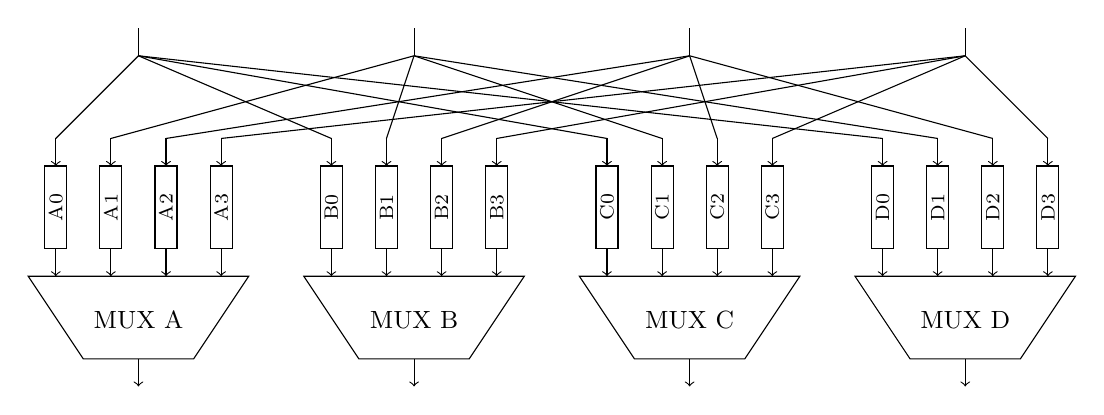
\begin{tikzpicture}[scale=.7]
            \foreach \i/\l in {0/A, 5/B, 10/C, 15/D}{
                \draw[xshift=\i cm] (-2,1) -- (2,1) -- (1,-.5) -- (-1,-.5) -- cycle;
                \node at (\i,.2){\small MUX \l};
                \draw [xshift=\i cm,->](0,-.5) -- (0,-1);
                \foreach \j/\p in {-1.5/0, -.5/1, .5/2,1.5/3}{
                    \draw [xshift = \i cm](\j-.2,1.5) rectangle (\j+.2,3);
                    \node at (\i+\j,2.25)[rotate=90]{\scriptsize \l\p};
                    \draw [xshift = \i cm,->](\j,1.5) -- (\j,1);
                    \draw [xshift = \i cm,->](\j,3.5) -- (\j,3);
                }
            }
            \foreach \i/\j in {0/-1.5, 5/-.5, 10/.5, 15/1.5}{
                \foreach \k in {0, 5, 10, 15}{
                    \draw (\i, 5) -- (\k+\j, 3.5);
                }
                \draw (\i,5) -- (\i, 5.5);
            }
        \end{tikzpicture}
        \caption{The fully-connected interconnect network.}
        \label{fig:crossbar}
    \end{figure}

    A straight forward way to create this memory would use full-connected interconnect networks (\figurename~\ref{fig:crossbar}). Unfortunately, as the size of a fully-connected interconnect network grows, the more space the FIFOs and multiplexers require. A 8-to-1 multiplexer requires approximately twice the number of resources of a 4-to-1 multiplexer. This means the area the multiplexers require grows by around $N^2$. The number of FIFOs grows by $N^2$ as well.

\section{Omega Multi-port Memory}
    \begin{figure}
        \center
        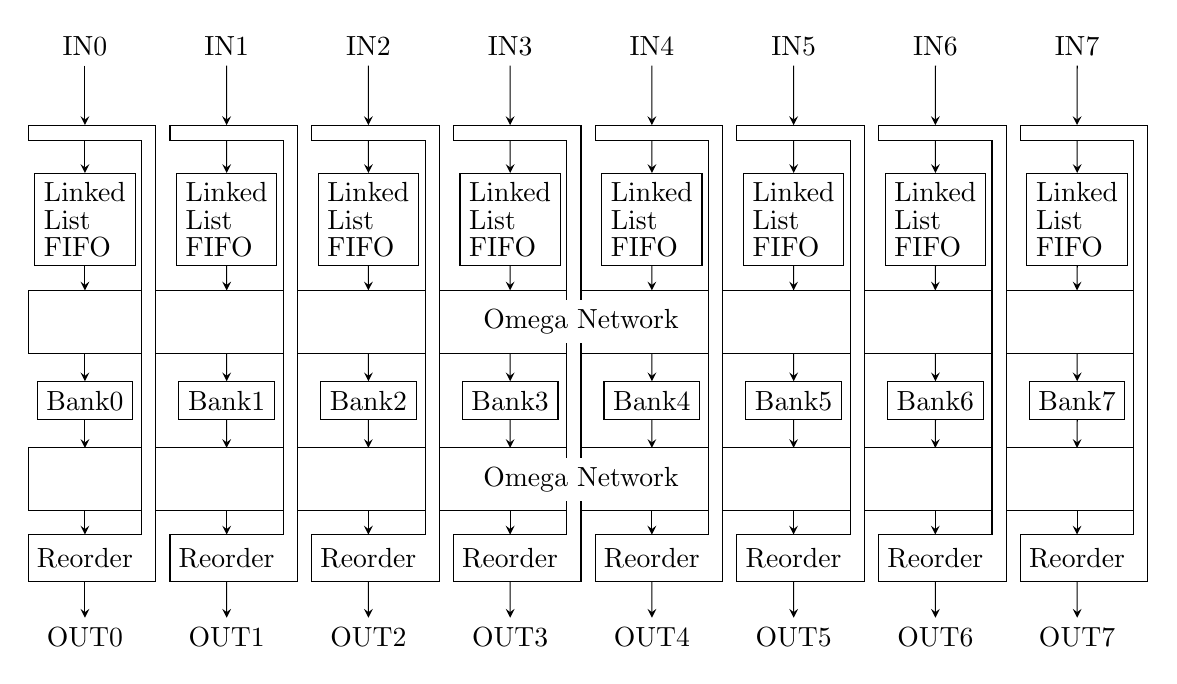
\begin{tikzpicture}[xscale=1.8]
            \draw (-.4,-1.6) rectangle (7.4,-2.4);
            \draw (-.4,-3.6) rectangle (7.4,-4.4);
            %\draw[dashed] (-.5,0) rectangle (3.5,-4.5);
            \foreach \x in {0,1,...,7}{
                \node at (\x,1.5)(in){IN\x};
                \node at (\x,-6)(out){OUT\x};
                \draw[xshift=\x cm - .1 cm,fill=white](-.3,.5) -- (-.3,.3) -- (.5,.3) -- (.5,-4.7) -- (-.3,-4.7) -- (-.3,-5.3) -- (.6,-5.3) -- (.6, .5) -- cycle;
                \node at (\x, -5){Reorder};
                \node[draw] at (\x,-.7)(inBuf){\shortstack[l]{Linked\\List\\FIFO}};
                \node[draw] at (\x,-3)(mem){Bank\x};
                \path[draw,>=stealth,->] (in) -- (\x,.5);
                \path[draw,>=stealth,->] (\x,.3) -- (inBuf);
                \path[draw,>=stealth,->] (inBuf) -- (\x,-1.6);
                \path[draw,>=stealth,->] (\x,-2.4) -- (mem);
                \path[draw,>=stealth,->] (mem) -- (\x,-3.6);
                \path[draw,>=stealth,->] (\x,-4.4) -- (\x,-4.7);
                \path[draw,>=stealth,->] (\x,-5.3) -- (out);
            }
            \node[fill=white] at (3.5,-2){Omega Network};
            \node[fill=white] at (3.5,-4){Omega Network};
            %\node[xshift=-3,rotate=90,fill=white] at (-.5,-2){Multi-port Memory};

        \end{tikzpicture}
        \caption[The Omega multi-port memory.]{In the Omega multi-port memory all the buffering occurs in the linked list FIFOs. The use of multi-stage interconnect networks, in this case Omega networks, helps reduce the area of the design.}
        \label{fig:versionb}
    \end{figure}
    The Omega multi-port memory (\figurename~\ref{fig:versionb}) has hardware structures designed for scaling. Instead of using fully connected interconnect networks, area efficient multi-stage interconnect networks (MIN) route signals to and from the memory banks. In addition, this memory uses $N$ linked list FIFOs to buffer incoming requests, instead of $N^2$ FIFOs. These two structures pair well, because they both save logic resources. However, both share a common restriction; neither structure can simultaneously send multiple buffered messages, from the same port, to different banks.\par
    The Omega memory has several subcomponents: first, the memory banks for storing the data, second, Omega networks for routing between the ports and banks, third, linked list FIFOs to buffer requests to banks, fourth, reorder queues to reorder read responses.
\subsection{Memory Banks}
For any banking approach, a memory with $N$ ports requires at least $N$ RAM blocks. Each RAM block holds a unique segment of the total memory space. We have multiple options to decide how to segment the memory space. The simplest option assigns the first $N^{th}$ of the address space to Bank0, the next $N^{th}$ to Bank1, and so on. However, this approach can easily cause bottlenecks. For example, assume all the processing elements start to read from a low address located in Bank0 and continue to sequentially increment the read addresses. All the requests would route to Bank0, necessitating multiple stalls. The interleaving memory address space that our design uses decreases the chance these specific types of bottlenecks occur.
\subsection{Omega Network}
%    \begin{figure}
%        \center
%        \begin{subfigure}{.32\linewidth}
%        \center
%        \input{fig/banyan1.tex}
%        \caption{Banyan Switch}
%        \label{fig:banyan}
%    \end{subfigure}
%        \begin{subfigure}{.32\linewidth}
%        \center
%        \input{fig/banyanon.tex}
%        \caption{Banyan Switch in the on state}
%        \label{fig:banyanon}
%    \end{subfigure}
%        \begin{subfigure}{.32\linewidth}
%        \center
%        \input{fig/banyanoff.tex}
%        \caption{Banyan Switch in the off state}
%        \label{fig:banyanoff}
%    \end{subfigure}
%    \caption{}
%    \end{figure}
    \begin{figure}
        \center

        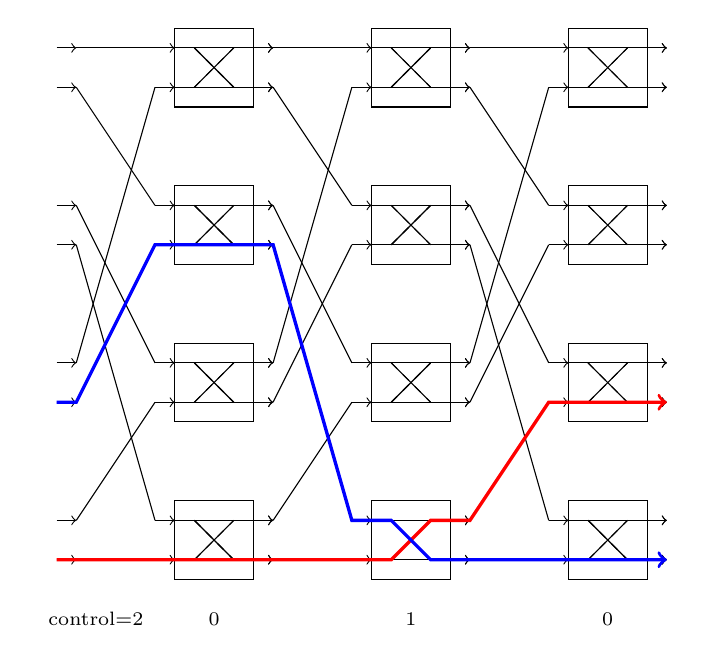
\begin{tikzpicture}[scale = .5]
            \foreach \i/\on in {0/0, 5/1, 10/0}{
                \foreach \j in {0, 4, 8, 12}{
                    \draw [shift={(\i,\j)}](-1,-1) rectangle (1,1);
                    \draw [shift={(\i,\j)}][->] (-1.5,-.5) -- (-1,-.5);
                    \draw [shift={(\i,\j)}][->] (-1.5,.5) -- (-1,.5);
                    \ifthenelse{\on=1}{
                        \draw [shift={(\i,\j)}](-.5,-.5) -- (.5,.5);
                        \draw [shift={(\i,\j)}](-.5,.5) -- (.5,-.5);
                        \draw [shift={(\i,\j)}] (-1,-.5) -- (-.5,-.5);
                        \draw [shift={(\i,\j)}] (-1,.5) -- (-.5,.5);
                        \draw [shift={(\i,\j)}][->] (.5,-.5) -- (1.5,-.5);
                        \draw [shift={(\i,\j)}][->] (.5,.5) -- (1.5,.5);
                        \draw [dashed,shift={(\i,\j)}](-.5,-.5) -- (.5,-.5);
                        \draw [dashed,shift={(\i,\j)}](-.5,.5) -- (.5,.5);
                    }{
                        \draw [shift={(\i,\j)}][->] (-1,-.5) -- (1.5,-.5);
                        \draw [shift={(\i,\j)}][->] (-1,.5) -- (1.5,.5);
                        \draw [dashed,shift={(\i,\j)}](-.5,-.5) -- (.5,.5);
                        \draw [dashed,shift={(\i,\j)}](-.5,.5) -- (.5,-.5);
                    }
                }
                \foreach \j/\k in {-.5/-.5,.5/3.5, 3.5/7.5, 4.5/11.5}{
                    \draw (\i-3.5, \j) -- (\i-1.5, \k);
                }
                \foreach \j/\k in {7.5/.5,8.5/4.5, 11.5/8.5, 12.5/12.5}{
                    \draw (\i-3.5, \j) -- (\i-1.5, \k);
                }
            }
            \foreach \i in {-.5,.5, 3.5,4.5, 7.5,8.5, 11.5,12.5}{
                \draw [->](-4,\i) -- (-3.5,\i);
            }
            \path[draw,red,very thick,->] (-4,-.5) -- (4.5,-.5) -- ++(1,1) -- ++(1,0) -- ++(2,3) -- ++(3,0);
            \path[draw,blue,very thick,->] (-4,3.5) -- ++(.5,0) -- ++(2,4) -- ++(3,0) -- ++(2,-7) -- ++(1,0) -- ++(1,-1) -- ++(6,0);
            \foreach [count=\c] \i in {-.5,.5, 3.5,4.5, 7.5,8.5, 11.5,12.5}{
                \FPeval{\z}{round(\c-1:0)};
                \node at (-4.5,\i) {\scriptsize \z};
                \node at (12,\i) {\scriptsize \z};
            }
            \node at (0,-2) {\scriptsize 0};
            \node at (5,-2) {\scriptsize 1};
            \node at (10,-2) {\scriptsize 0};
            \node at (-3,-2) {\scriptsize control=2};
        \end{tikzpicture}
        \caption[The Omega network.]{An 8-by-8 Omega network. We turn columns on or off to rotate between different routing configurations.}
        \label{fig:omega010}
    \end{figure}

    An Omega network consists of columns of Banyan switches~\cite{prelim:wu,prelim:lawrie}. A Banyan switch synthesizes to two multiplexers. In the on state, the switch crosses data over to the opposite output port. As an illustrative example, the second column in \figurename~\ref{fig:omega010} only contains switches in the on state. In the off state, the switch passes data straight to the corresponding output port. The first and last columns in \figurename~\ref{fig:omega010} only contain switches in the off state.

The Omega network has features that make it attractive in a multi-port memory design. If we switch whole columns of Banyan switches on or off, we can easily determine where signals route by XORing the starting port index with the bits controlling the columns. For example, in \figurename~\ref{fig:omega010}, the control bits equal $010_2$ or 2 and input port 2 ($010_2$) routes to output port 0. Not coincidentally, the same configuration routes in reverse. Input port 0 routes to output port 2 and input port 2 routes to output port 0. This means the design can use identical control bits for both the receiving and sending Omega networks.

In the Omega multi-port memory design, the control for this network increments every clock cycle. As an example, input port 5 would connect to output port 5, then port 4, 7, 6, 1, etc., until it cycles around again. This means each input connects to each output an equal number of times.

\subsection{The Linked List FIFO}
\label{sec:linkedfifo}
    \begin{figure}
        \center
        \begin{subfigure}{.4\linewidth}
        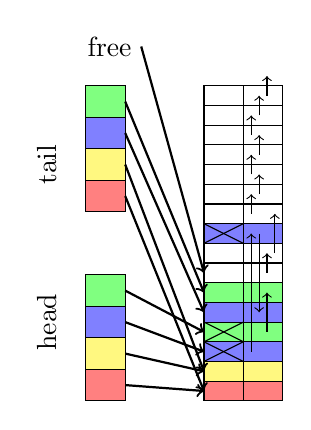
\begin{tikzpicture}
        \fill [red!50] (-.5,-2) rectangle (.5,-1.75);
        \fill [yellow!50] (-.5,-1.75) rectangle (.5,-1.5);
        \fill [blue!50] (-.5,-1.5) rectangle (.5,-1.25);
        \fill [blue!50] (-.5,-1) rectangle (.5,-.75);
        \fill [blue!50] (-.5,0) rectangle (.5,.25);
        \fill [green!50] (-.5,-1.25) rectangle (.5,-1);
        \fill [green!50] (-.5,-.5) rectangle (.5,-.75);
        \draw (-.5,-2) rectangle (0,2);
        \draw (0,-2) rectangle (.5,2);
        \foreach \i in {-1.75,-1.5,...,1.75}{
            \draw (-.5,\i) -- (.5,\i);
        }
        \node at (-2.5,-1)[rotate=90]{head};
        \node at (-2.5,1)[rotate=90]{tail};
        \node (f) at (-1.7,2.5) {free};
        \fill [red!50] (-2,-2) rectangle (-1.5,-1.6);
        \fill [yellow!50] (-2,-1.6) rectangle (-1.5,-1.2);
        \fill [blue!50] (-2,-1.2) rectangle (-1.5,-.8);
        \fill [green!50] (-2,-.8) rectangle (-1.5,-.4);
        \fill [red!50] (-2,.4) rectangle (-1.5,.8);
        \fill [yellow!50] (-2,.8) rectangle (-1.5,1.2);
        \fill [blue!50] (-2,1.2) rectangle (-1.5,1.6);
        \fill [green!50] (-2,1.6) rectangle (-1.5,2);
        \draw (-2,-2) rectangle (-1.5, -.4);
        \draw (-2,2) rectangle (-1.5, .4);
        \foreach \i in {-1.6,-1.2,-.8,.8,1.2,1.6}{
            \draw (-2,\i) -- (-1.5,\i);
        }
        \foreach[count=\i] \l/\h in {0/0,1/1,2/4,3/5}{
            \draw [thick,->] (-1.5,-1.8+\i*.4-.4) -- (-.5,\l*.25-1.875);
            \draw [thick,->] (-1.5,.6+\i*.4-.4) -- (-.5,\h*.25-1.875);
        }
        \draw (-.5,-1.5) -- (0,-1.25);
        \draw (-.5,-1.25) -- (0,-1.5);
        \draw (-.5,-1.25) -- (0,-1);
        \draw (-.5,-1) -- (0,-1.25);
        \draw (-.5,.25) -- (0,0);
        \draw (-.5,0) -- (0,.25);
        \draw [thick,->] (f.east) -- (-.5,-.375);
        \draw [->] (.1,-1.375) -- (.1,.125);
        \draw [->] (.2,.125) -- (.2,-.875);
        \draw [->] (.3,-.375) -- (.3,-.125);
        \draw [->] (.4,-.125) -- (.4,.375);
        \draw [->] (.3,-1.125) -- (.3,-.625);
        \foreach \i in {.375,.875,...,1.625}{
            \draw [->] (.1,\i) -- (.1,\i+.25);
            \draw [->] (.2,\i+.25) -- (.2,\i+.5);
        }
        \draw [->] (.3,1.875) -- (.3,2.125);

        \end{tikzpicture}
        \caption{Initial example}
        \label{fig:linked0}
    \end{subfigure}
        \begin{subfigure}{.4\linewidth}

        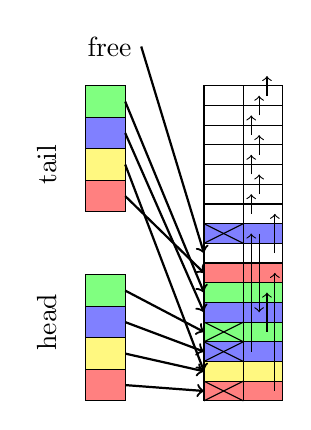
\begin{tikzpicture}
        \fill [red!50] (-.5,-2) rectangle (.5,-1.75);
        \fill [red!50] (-.5,-.5) rectangle (.5,-.25);
        \fill [yellow!50] (-.5,-1.75) rectangle (.5,-1.5);
        \fill [blue!50] (-.5,-1.5) rectangle (.5,-1.25);
        \fill [blue!50] (-.5,-1) rectangle (.5,-.75);
        \fill [blue!50] (-.5,0) rectangle (.5,.25);
        \fill [green!50] (-.5,-1.25) rectangle (.5,-1);
        \fill [green!50] (-.5,-.5) rectangle (.5,-.75);
        \draw (-.5,-2) rectangle (0,2);
        \draw (0,-2) rectangle (.5,2);
        \foreach \i in {-1.75,-1.5,...,1.75}{
            \draw (-.5,\i) -- (.5,\i);
        }
        \node at (-2.5,-1)[rotate=90]{head};
        \node at (-2.5,1)[rotate=90]{tail};
        \node (f) at (-1.7,2.5) {free};
        \fill [red!50] (-2,-2) rectangle (-1.5,-1.6);
        \fill [yellow!50] (-2,-1.6) rectangle (-1.5,-1.2);
        \fill [blue!50] (-2,-1.2) rectangle (-1.5,-.8);
        \fill [green!50] (-2,-.8) rectangle (-1.5,-.4);
        \fill [red!50] (-2,.4) rectangle (-1.5,.8);
        \fill [yellow!50] (-2,.8) rectangle (-1.5,1.2);
        \fill [blue!50] (-2,1.2) rectangle (-1.5,1.6);
        \fill [green!50] (-2,1.6) rectangle (-1.5,2);
        \draw (-2,-2) rectangle (-1.5, -.4);
        \draw (-2,2) rectangle (-1.5, .4);
        \foreach \i in {-1.6,-1.2,-.8,.8,1.2,1.6}{
            \draw (-2,\i) -- (-1.5,\i);
        }
        \foreach[count=\i] \l/\h in {0/6,1/1,2/4,3/5}{
            \draw [thick,->] (-1.5,-1.8+\i*.4-.4) -- (-.5,\l*.25-1.875);
            \draw [thick,->] (-1.5,.6+\i*.4-.4) -- (-.5,\h*.25-1.875);
        }
        \draw (-.5,-2) -- (0,-1.75);
        \draw (-.5,-1.75) -- (0,-2);
        \draw (-.5,-1.5) -- (0,-1.25);
        \draw (-.5,-1.25) -- (0,-1.5);
        \draw (-.5,-1.25) -- (0,-1);
        \draw (-.5,-1) -- (0,-1.25);
        \draw (-.5,.25) -- (0,0);
        \draw (-.5,0) -- (0,.25);
        \draw [thick,->] (f.east) -- (-.5,-.125);
        \draw [->] (.1,-1.375) -- (.1,.125);
        \draw [->] (.2,.125) -- (.2,-.875);
        \draw [->] (.4,-1.875) -- (.4,-.375);
        \draw [->] (.4,-.125) -- (.4,.375);
        \draw [->] (.3,-1.125) -- (.3,-.625);
        \foreach \i in {.375,.875,...,1.625}{
            \draw [->] (.1,\i) -- (.1,\i+.25);
            \draw [->] (.2,\i+.25) -- (.2,\i+.5);
        }
        \draw [->] (.3,1.875) -- (.3,2.125);

        \end{tikzpicture}
        \caption{First clock cycle}
        \label{fig:linked1}
    \end{subfigure}
        \begin{subfigure}{.4\linewidth}

        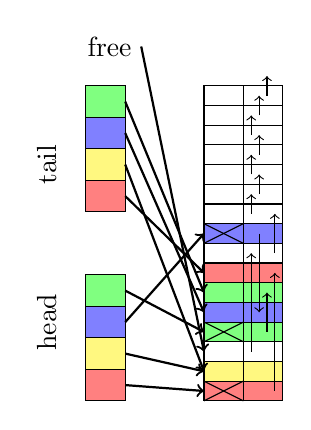
\begin{tikzpicture}
        \fill [red!50] (-.5,-2) rectangle (.5,-1.75);
        \fill [red!50] (-.5,-.5) rectangle (.5,-.25);
        \fill [yellow!50] (-.5,-1.75) rectangle (.5,-1.5);
        \fill [blue!50] (-.5,-1) rectangle (.5,-.75);
        \fill [blue!50] (-.5,0) rectangle (.5,.25);
        \fill [green!50] (-.5,-1.25) rectangle (.5,-1);
        \fill [green!50] (-.5,-.5) rectangle (.5,-.75);
        \draw (-.5,-2) rectangle (0,2);
        \draw (0,-2) rectangle (.5,2);
        \foreach \i in {-1.75,-1.5,...,1.75}{
            \draw (-.5,\i) -- (.5,\i);
        }
        \node at (-2.5,-1)[rotate=90]{head};
        \node at (-2.5,1)[rotate=90]{tail};
        \node (f) at (-1.7,2.5) {free};
        \fill [red!50] (-2,-2) rectangle (-1.5,-1.6);
        \fill [yellow!50] (-2,-1.6) rectangle (-1.5,-1.2);
        \fill [blue!50] (-2,-1.2) rectangle (-1.5,-.8);
        \fill [green!50] (-2,-.8) rectangle (-1.5,-.4);
        \fill [red!50] (-2,.4) rectangle (-1.5,.8);
        \fill [yellow!50] (-2,.8) rectangle (-1.5,1.2);
        \fill [blue!50] (-2,1.2) rectangle (-1.5,1.6);
        \fill [green!50] (-2,1.6) rectangle (-1.5,2);
        \draw (-2,-2) rectangle (-1.5, -.4);
        \draw (-2,2) rectangle (-1.5, .4);
        \foreach \i in {-1.6,-1.2,-.8,.8,1.2,1.6}{
            \draw (-2,\i) -- (-1.5,\i);
        }
        \foreach[count=\i] \l/\h in {0/6,1/1,8/4,3/5}{
            \draw [thick,->] (-1.5,-1.8+\i*.4-.4) -- (-.5,\l*.25-1.875);
            \draw [thick,->] (-1.5,.6+\i*.4-.4) -- (-.5,\h*.25-1.875);
        }
        \draw (-.5,-2) -- (0,-1.75);
        \draw (-.5,-1.75) -- (0,-2);
        \draw (-.5,-1.25) -- (0,-1);
        \draw (-.5,-1) -- (0,-1.25);
        \draw (-.5,.25) -- (0,0);
        \draw (-.5,0) -- (0,.25);
        \draw [thick,->] (f.east) -- (-.5,-1.375);
        \draw [->] (.1,-1.375) -- (.1,-.125);
        \draw [->] (.2,.125) -- (.2,-.875);
        \draw [->] (.4,-1.875) -- (.4,-.375);
        \draw [->] (.4,-.125) -- (.4,.375);
        \draw [->] (.3,-1.125) -- (.3,-.625);
        \foreach \i in {.375,.875,...,1.625}{
            \draw [->] (.1,\i) -- (.1,\i+.25);
            \draw [->] (.2,\i+.25) -- (.2,\i+.5);
        }
        \draw [->] (.3,1.875) -- (.3,2.125);

        \end{tikzpicture}
        \caption{Second clock cycle}
        \label{fig:linked2}
    \end{subfigure}
        \begin{subfigure}{.4\linewidth}
        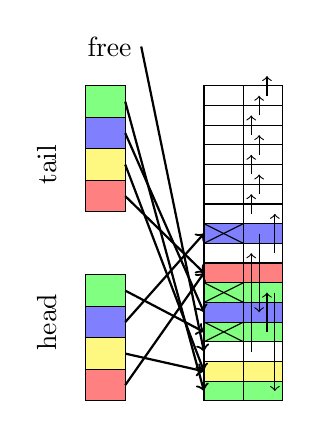
\begin{tikzpicture}
        \fill [green!50] (-.5,-2) rectangle (.5,-1.75);
        \fill [red!50] (-.5,-.5) rectangle (.5,-.25);
        \fill [yellow!50] (-.5,-1.75) rectangle (.5,-1.5);
        \fill [blue!50] (-.5,-1) rectangle (.5,-.75);
        \fill [blue!50] (-.5,0) rectangle (.5,.25);
        \fill [green!50] (-.5,-1.25) rectangle (.5,-1);
        \fill [green!50] (-.5,-.5) rectangle (.5,-.75);
        \draw (-.5,-2) rectangle (0,2);
        \draw (0,-2) rectangle (.5,2);
        \foreach \i in {-1.75,-1.5,...,1.75}{
            \draw (-.5,\i) -- (.5,\i);
        }
        \node at (-2.5,-1)[rotate=90]{head};
        \node at (-2.5,1)[rotate=90]{tail};
        \node (f) at (-1.7,2.5) {free};
        \fill [red!50] (-2,-2) rectangle (-1.5,-1.6);
        \fill [yellow!50] (-2,-1.6) rectangle (-1.5,-1.2);
        \fill [blue!50] (-2,-1.2) rectangle (-1.5,-.8);
        \fill [green!50] (-2,-.8) rectangle (-1.5,-.4);
        \fill [red!50] (-2,.4) rectangle (-1.5,.8);
        \fill [yellow!50] (-2,.8) rectangle (-1.5,1.2);
        \fill [blue!50] (-2,1.2) rectangle (-1.5,1.6);
        \fill [green!50] (-2,1.6) rectangle (-1.5,2);
        \draw (-2,-2) rectangle (-1.5, -.4);
        \draw (-2,2) rectangle (-1.5, .4);
        \foreach \i in {-1.6,-1.2,-.8,.8,1.2,1.6}{
            \draw (-2,\i) -- (-1.5,\i);
        }
        \foreach[count=\i] \l/\h in {6/6,1/1,8/4,3/0}{
            \draw [thick,->] (-1.5,-1.8+\i*.4-.4) -- (-.5,\l*.25-1.875);
            \draw [thick,->] (-1.5,.6+\i*.4-.4) -- (-.5,\h*.25-1.875);
        }
        \draw (-.5,-.75) -- (0,-.5);
        \draw (-.5,-.5) -- (0,-.75);
        \draw (-.5,-1.25) -- (0,-1);
        \draw (-.5,-1) -- (0,-1.25);
        \draw (-.5,.25) -- (0,0);
        \draw (-.5,0) -- (0,.25);
        \draw [thick,->] (f.east) -- (-.5,-1.375);
        \draw [->] (.1,-1.375) -- (.1,-.125);
        \draw [->] (.2,.125) -- (.2,-.875);
        \draw [->] (.4,-.625) -- (.4,-1.875);
        \draw [->] (.4,-.125) -- (.4,.375);
        \draw [->] (.3,-1.125) -- (.3,-.625);
        \foreach \i in {.375,.875,...,1.625}{
            \draw [->] (.1,\i) -- (.1,\i+.25);
            \draw [->] (.2,\i+.25) -- (.2,\i+.5);
        }
        \draw [->] (.3,1.875) -- (.3,2.125);

        \end{tikzpicture}
        \caption{Third clock cycle}
        \label{fig:linked3}
    \end{subfigure}
    \caption[The linked list FIFO.]{A linked list FIFO during 3 clock cycles of operation}
        \label{fig:linkedfifo}
    \end{figure}
    The partnering hardware structure, the linked list FIFO (\figurename~\ref{fig:linkedfifo}), contains several internal FIFOs with no predefined space in a single RAM. Similar to a software linked list, there exists a free pointer that points to the beginning of the free space linked list. Other variants of hardware linked list FIFOs exist [\cite{prelim:bell2,prelim:nikologiannis}].

    Due to the linking pointers, the size of the RAM now needs $O(N\log N)$ space to store $N$ elements. However $\log N$ grows slowly. For example, data stored in a 64-bit wide by 1024 deep RAM would need an additional 11-bit wide by 1024 deep RAM for the linking pointers. An illustrative example of the linked list FIFO is shown in in \figurename~\ref{fig:linkedfifo}, which uses a 16 deep RAM and 4 FIFOs.

    In the initial state (\figurename~\ref{fig:linked0}), the red and yellow FIFOs have no messages. The blue FIFO has two messages. And, the green FIFO has one message. However, every FIFO reserves one space for the next incoming value. This limits the total available space in the linked list FIFO to $TOTAL\_DEPTH-FIFO\_COUNT$.

         On the first clock cycle (\figurename~\ref{fig:linked1}), the linked list FIFO receives a push containing a red message. The new red message gets stored in the reserved space at the tail of the red linked list. The free linked list pops one space. That space gets pushed on to the red linked list.

         On the second clock cycle (\figurename~\ref{fig:linked2}), the linked list FIFO receives a pop for a blue message. A blue message gets popped from the head of the blue linked list. The newly freed space gets pushed on to the free linked list.

         On the third clock cycle (\figurename~\ref{fig:linked3}), the linked list receives a pop for a red message and a push for a green message. In this case, the space that the red message was popped from gets pushed onto the green linked list. The free space linked list stays the same.

\subsection{Reorder Queue}
    \begin{figure}
        \center
        \begin{subfigure}{.32\linewidth}
            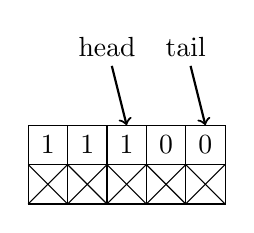
\begin{tikzpicture}
                \draw (0,0) rectangle (2.5,1);
                \draw (0,.5) -- (2.5,.5);
            \foreach \i in {.5,1,...,2}{
                \draw (\i,0) -- (\i,1);
            }
            \foreach \i/\j/\k in {0/1/0,1/1/0,2/1/1,3/0/0,4/0/0}{
                \node at (\i*.5+.25,.75) {\j};
                \ifthenelse{\k=1}{
                    \draw (\i*.5,0) -- (\i*.5+.5,.5);
                    \draw (\i*.5,.5) -- (\i*.5+.5,0);
                }{};
            }
            \node at (1,2) (b) {head};
            \node at (2,2) (e) {tail};
            \draw [thick,->] (b) -- (1.25,1);
            \draw [thick,->] (e) -- (2.25,1);

            \end{tikzpicture}
            \caption{Initial example}
            \label{fig:reorder0}
        \end{subfigure}
        \begin{subfigure}{.32\linewidth}
            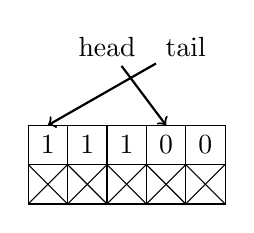
\begin{tikzpicture}
                \draw (0,0) rectangle (2.5,1);
                \draw (0,.5) -- (2.5,.5);
            \foreach \i in {.5,1,...,2}{
                \draw (\i,0) -- (\i,1);
            }
            \foreach \i/\j/\k in {0/1/0,1/1/0,2/1/0,3/0/0,4/0/0}{
                \node at (\i*.5+.25,.75) {\j};
                \ifthenelse{\k=1}{
                    \draw (\i*.5,0) -- (\i*.5+.5,.5);
                    \draw (\i*.5,.5) -- (\i*.5+.5,0);
                }{};
            }
            \node at (1,2) (b) {head};
            \node at (2,2) (e) {tail};
            \draw [thick,->] (b) -- (1.75,1);
            \draw [thick,->] (e) -- (.25,1);

            \end{tikzpicture}
            \caption{First clock cycle}
            \label{fig:reorder1}
        \end{subfigure}
        \begin{subfigure}{.32\linewidth}
            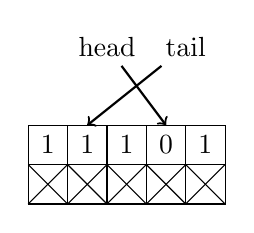
\begin{tikzpicture}
                \draw (0,0) rectangle (2.5,1);
                \draw (0,.5) -- (2.5,.5);
            \foreach \i in {.5,1,...,2}{
                \draw (\i,0) -- (\i,1);
            }
            \foreach \i/\j/\k in {0/1/0,1/1/0,2/1/0,3/0/0,4/1/1}{
                \node at (\i*.5+.25,.75) {\j};
                \ifthenelse{\k=1}{
                    \draw (\i*.5,0) -- (\i*.5+.5,.5);
                    \draw (\i*.5,.5) -- (\i*.5+.5,0);
                }{};
            }
            \node at (1,2) (b) {head};
            \node at (2,2) (e) {tail};
            \draw [thick,->] (b) -- (1.75,1);
            \draw [thick,->] (e) -- (.75,1);

            \end{tikzpicture}
            \caption{Second clock cycle}
            \label{fig:reorder2}
        \end{subfigure}
        \begin{subfigure}{.32\linewidth}
            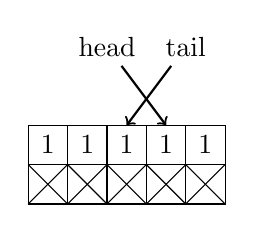
\begin{tikzpicture}
                \draw (0,0) rectangle (2.5,1);
                \draw (0,.5) -- (2.5,.5);
            \foreach \i in {.5,1,...,2}{
                \draw (\i,0) -- (\i,1);
            }
            \foreach \i/\j/\k in {0/1/0,1/1/0,2/1/0,3/1/1,4/1/1}{
                \node at (\i*.5+.25,.75) {\j};
                \ifthenelse{\k=1}{
                    \draw (\i*.5,0) -- (\i*.5+.5,.5);
                    \draw (\i*.5,.5) -- (\i*.5+.5,0);
                }{};
            }
            \node at (1,2) (b) {head};
            \node at (2,2) (e) {tail};
            \draw [thick,->] (b) -- (1.75,1);
            \draw [thick,->] (e) -- (1.25,1);

            \end{tikzpicture}
            \caption{Third clock cycle}
            \label{fig:reorder3}
        \end{subfigure}
        \begin{subfigure}{.32\linewidth}
            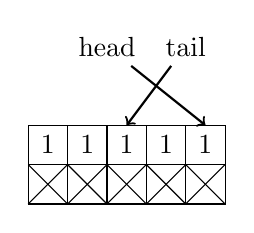
\begin{tikzpicture}
                \draw (0,0) rectangle (2.5,1);
                \draw (0,.5) -- (2.5,.5);
            \foreach \i in {.5,1,...,2}{
                \draw (\i,0) -- (\i,1);
            }
            \foreach \i/\j/\k in {0/1/0,1/1/0,2/1/0,3/1/0,4/1/1}{
                \node at (\i*.5+.25,.75) {\j};
                \ifthenelse{\k=1}{
                    \draw (\i*.5,0) -- (\i*.5+.5,.5);
                    \draw (\i*.5,.5) -- (\i*.5+.5,0);
                }{};
            }
            \node at (1,2) (b) {head};
            \node at (2,2) (e) {tail};
            \draw [thick,->] (b) -- (2.25,1);
            \draw [thick,->] (e) -- (1.25,1);

            \end{tikzpicture}
            \caption{Fourth clock cycle}
            \label{fig:reorder4}
        \end{subfigure}
        \begin{subfigure}{.32\linewidth}
            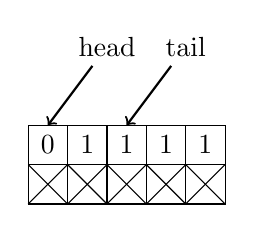
\begin{tikzpicture}
                \draw (0,0) rectangle (2.5,1);
                \draw (0,.5) -- (2.5,.5);
            \foreach \i in {.5,1,...,2}{
                \draw (\i,0) -- (\i,1);
            }
            \foreach \i/\j/\k in {0/0/1,1/1/0,2/1/0,3/1/0,4/1/0}{
                \node at (\i*.5+.25,.75) {\j};
                \ifthenelse{\k=1}{
                    \draw (\i*.5,0) -- (\i*.5+.5,.5);
                    \draw (\i*.5,.5) -- (\i*.5+.5,0);
                }{};
            }
            \node at (1,2) (b) {head};
            \node at (2,2) (e) {tail};
            \draw [thick,->] (b) -- (.25,1);
            \draw [thick,->] (e) -- (1.25,1);

            \end{tikzpicture}
            \caption{Fifth clock cycle}
            \label{fig:reorder5}
        \end{subfigure}
        %\input{fig/reorder.tex}
        \caption[The reorder queue]{Reorder queue example.}
        \label{fig:reorder}
    \end{figure}

    The buffering in both designs ensures relatively high throughput, however, this buffering causes a problem for both memories, as read responses from different banks from the same port may come back out of order. Although out of order reads do not always cause an issue, to alleviate this issue we add reorder queues to both multi-port memory designs.

    A reorder queue behaves similarly to a FIFO. However, some of the values in between the head and tail pointer exist ``in flight'' and not at the reorder queue memory. The reorder queue keeps track of the presence of messages with a bit array (a 1-bit wide RAM).

    \figurename~\ref{fig:reorder} shows an example with 5 clock cycles of operation. In the initial state (\figurename~\ref{fig:reorder0}), the reorder queue has one present message and one in flight message.

         On the first clock cycle (\figurename~\ref{fig:reorder1}), the present message at the head gets popped from the queue. A new message increments the tail, but the message remains in flight until it arrives at the reorder queue.

         On the second clock cycle (\figurename~\ref{fig:reorder2}), a new message arrives at the reorder queue, however, it does not arrive at the head of the queue so no message can get popped.

         On the third clock cycle (\figurename~\ref{fig:reorder3}), a message arrives at the head of the reorder queue.

         On the fourth clock cycle (\figurename~\ref{fig:reorder4}), this message at the head of the reorder queue gets popped. If the reorder queue did not exist, the message that appeared on clock cycle 2 would have reached the output first even though it was sent later.

         On the fifth clock cycle (\figurename~\ref{fig:reorder5}), a message arrives. However, the meaning of 1 or 0 in the 1-bit RAM switched after the pointers wrapped around the end of the RAM. Instead of 1 meaning present, 1 now means in flight. This semantic flipping allows the use of only one write port on the 1-bit RAM (instead of two if the bits flipped after popping a message), saving on memory-related resources. 

\section{Evaluation}
\label{sec:evaluation}
    We limit linked list FIFOs and reorder queues to a depth of 64. We limit the depth of the FIFOs in the fully-connected interconnect network to 32 since the number of FIFOs in it grows by $O(N^2)$.

    We used the ModelSim logic simulator to evaluate the performance of each configuration. The testbench used for evaluation consists of four benchmarks. Each benchmark tests the read performance of sequential, random, congested, or segregated memory access patterns.

    We calculate the throughput of a given benchmark by measuring the ratio of read requests to potential read requests. If no stalls occur, the throughput equals 100\%. We calculate the latency by measuring the number of clock cycles between the last read request and the last read response. 
\begin{table*}
    \center
    \caption{Analysis of the Omega multi-port memory design.}
    \label{tbl:resources}
\begin{threeparttable}
\begin{tabular}{|l|l|l|l|l|l|}
\hline
Ports & & 4 & 8 & 16 & 32 \\
Memory Space & &  16KB & 32KB & 64KB & 128KB \\
\hline
 & \multicolumn{5}{|c|}{Fully-connected Multi-port Memory}\\
\cline{1-6}
\multirow{4}{*}{\shortstack[l]{Resource\\Utilization\\Virtex 7\\ V2000T\tnote{2}}} & Registers & 4K & 14K & 50K & 190K \\
                                                                          & LUTs      & 5.7K & 18K & 61K & 241K \\
& BlockRAM  & 4 & 8 & 16 & 32 \\
 & Clock frequency & 345Mhz & 313Mhz & 256Mhz & 273Mhz \\
\hline
Sequential & Throughput & 100\% & 100\% & 100\% & 100\% \\
 & Latency \tnote{1} & 16 & 20 & 36 & 64 \\
Random & Throughput & 97\% & 93\% & 88\% & 72\% \\
 & Latency \tnote{1} & 66 & 65 & 85 & 97 \\
Congested & Throughput & 25\% & 13\% & 6\% & 3\% \\ 
 & Latency \tnote{1} & 105 & 230 & 490 & 1034 \\
Segregated & Throughput & 100\% & 100\% & 100\% & 100\% \\
 & Latency \tnote{1} & 16 & 24 & 34 & 63 \\
\hline
 & \multicolumn{5}{|c|}{Omega Multi-port Memory} \\
\hline
\multirow{4}{*}{\shortstack[l]{Resource\\Utilization\\Virtex 7\\ V2000T\tnote{2}}}& Registers & 3K & 9K & 22K & 53K \\
                                                                      & LUTs      & 5K & 11K & 24K & 53K \\
& BlockRAM  & 4 & 8 & 16 & 32 \\
& Clock frequency & 258Mhz & 257Mhz & 260Mhz & 262Mhz \\
\hline
Sequential & Throughput & 100\%  & 100\% & 100\% & 100\% \\
& Latency \tnote{1} & 17 & 25 & 37 & 56 \\
Random & Throughput & 94\% & 83\% & 68\% & 52\% \\
 & Latency \tnote{1} & 72 & 110 & 131 & 193 \\
Congested & Throughput & 25\% & 13\% & 6\% & 3\% \\
 & Latency \tnote{1} & 250 & 462 & 786 & 1046 \\
Segregated & Throughput & 25\% & 13\% & 6\% & 3\% \\
 & Latency \tnote{1} & 247 & 461 & 756 & 1043 \\
\hline
\end{tabular}
\begin{tablenotes}
\item[1] This measures the number of clock cycles between the end of the benchmark and when the last response of the last request gets received. In the worst case scenario several FIFOs queue data that has to wait for access to the same bank.
\item[2] This particular chip has 2.4M registers, 1.2M LUTs and 1.3K RAM blocks.
\end{tablenotes}
\end{threeparttable}
\end{table*}



\section{Results}
\label{sec:analysis}
\begin{figure}[t]
    \center
    \begin{tikzpicture}[xscale=.19,yscale=.07]
        \tikzstyle{blueSquare}=[draw, rectangle, fill=blue, inner sep =2.5pt];
        \tikzstyle{redCircle}=[draw, circle, fill=red, inner sep =2.1pt];
        \tikzstyle{greenDiamond}=[draw, diamond, fill=green, inner sep =1.8pt];
        \tikzstyle{blackTriangle}=[draw, regular polygon, regular polygon sides=3, fill=black, inner sep =1.6pt];
        \draw [->] (0,0) -- (40,0);
        \draw [->] (0,0) -- (0,100);
        \foreach \i in {4,8,16,32}{
            \draw (\i,1) -- (\i,-1)node[anchor=20,rotate=60]{\i};
        }
        \foreach \y in {20,40,...,80}{
            \FPeval{\v}{round(\y*2.5:0)};
            \draw (.4,\y) -- (-.4,\y)node[anchor=south,rotate=90]{\v K};
        }
        \node at (20, -10) {Ports};
        \node at (-4,50) [rotate=90]{LUTs/Registers};
\foreach \xa/\ya/\xb/\yb in {4/4.1/8/14.0,8/14.0/16/50.0,16/50.0/32/190.0}{
    \draw [thick, red] (\xa,\ya/2.5) -- (\xb,\yb/2.5);
}
\foreach \xa/\ya/\xb/\yb in {4/5.7/8/18.0,8/18.0/16/61.0,16/61.0/32/241.0}{
    \draw [thick, blue] (\xa,\ya/2.5) -- (\xb,\yb/2.5);
}
\foreach \xa/\ya/\xb/\yb in {4/3.1/8/8.5,8/8.5/16/22.1,16/22.1/32/52.7}{
    \draw [thick, black] (\xa,\ya/2.5) -- (\xb,\yb/2.5);
}
\foreach \xa/\ya/\xb/\yb in {4/4.9/8/10.9,8/10.9/16/24.0,16/24.0/32/53.0}{
    \draw [thick, green] (\xa,\ya/2.5) -- (\xb,\yb/2.5);
}
\foreach \x/\y/\a in {4/4.1/18,8/14.0/15,16/50.0/0,32/190.0/0}{
    \FPeval{\ys}{round(\y:0)}
    \node[redCircle] at (\x,\y/2.5) [label={[inner sep=0,xshift=3pt,red, fill=white, yshift=\a pt]0:\small \ys K}] {};
    %\node[draw,fill=red,circle,inner sep=1.5pt] at (\x,\y/2.5) [label={[inner sep=0,xshift=3pt,red, fill=white, yshift=\a pt]0:\small \ys K}] {};
}
\foreach \x/\y/\a in {4/5.7/25,8/18.0/20,16/61.0/0,32/241.0/0}{
    \FPeval{\ys}{round(\y:0)}
    \node[blueSquare] at (\x,\y/2.5) [label={[inner sep=0,xshift=3pt,blue, fill=white,yshift=\a pt]0:\small \ys K}] {};
    %\node[draw,fill=blue,inner sep=1.5pt] at (\x,\y/2.5) [label={[inner sep=0,xshift=3pt,blue, fill=white,yshift=\a pt]0:\small \ys K}] {};
}
\foreach \x/\y/\a in {4/3.1/0,8/8.5/0,16/22.1/0,32/52.7/0}{
    \FPeval{\ys}{round(\y:0)}
    %\node[draw,regular polygon, regular polygon sides=3,fill=black,inner sep=1.5pt] at (\x,\y/2.5) [label={[inner sep=0,xshift=3pt,black, fill=white,yshift=\a pt]0:\small \ys K}] {};
    \node[blackTriangle] at (\x,\y/2.5) [label={[inner sep=0,xshift=3pt,black, fill=white,yshift=\a pt]0:\small \ys K}] {};
}
\foreach \x/\y/\a in {4/4.9/8,8/10.9/8,16/24.0/8,32/53.0/8}{
    \FPeval{\ys}{round(\y:0)}
    \node[greenDiamond] at (\x,\y/2.5) [label={[inner sep=0,xshift=3pt,green, fill=white,yshift=\a pt]0:\small \ys K}] {};
    %\node[draw,diamond,fill=green,inner sep=1.5pt] at (\x,\y/2.5) [label={[inner sep=0,xshift=3pt,green, fill=white,yshift=\a pt]0:\small \ys K}] {};
}

        \node at (15,90) []{\shortstack[l]{\tikz \node[blueSquare] at (0,0) {}; Fully-connected LUTs\\
                                            \tikz \node[redCircle] at (0,0) {}; Fully-connected Registers\\
                                            \tikz \node[greenDiamond] at (0,0) {}; Omega LUTs\\
                                            \tikz \node[blackTriangle] at (0,0) {}; Omega Registers}};
    \end{tikzpicture}
    \caption[Graph showing the increase in resource utilization as the number of ports in the Omega memory increases.]{The effect of varying the number of ports on FPGA resource utilization (area). The Fully-connected memory grows by approximately $N^2$ and the Omega memory grows almost linearly.}
    \label{fig:portresources}
\end{figure}

\begin{figure}
    \center
    \begin{tikzpicture}[xscale=.19,yscale=.07]
        \tikzstyle{blueSquare}=[draw, rectangle, fill=blue, inner sep =2.5pt];
        \tikzstyle{redCircle}=[draw, circle, fill=red, inner sep =2.1pt];
        \tikzstyle{greenDiamond}=[draw, diamond, fill=green, inner sep =1.8pt];
        \tikzstyle{blackTriangle}=[draw, regular polygon, regular polygon sides=3, fill=black, inner sep =1.6pt];
        \draw [->] (0,0) -- (40,0);
        \draw (0,0) -- (0,100);
        \foreach \i in {4,8,16,32}{
            \draw (\i,1) -- (\i,-1)node[anchor=20,rotate=60]{\i};
        }
        \node at (20, -10) {Ports};
        \node at (-4,50) [rotate=90]{Throughput};
        \foreach \i in {20,40,...,100}{
            \draw (.4,\i) -- (-.4,\i) node[anchor=south,rotate=90]{\i\%};
        }
\foreach \xa/\ya/\xb/\yb in {4/96.5/8/93.5,8/93.5/16/87.7,16/87.7/32/72.0}{
    \draw [thick, blue] (\xa,\ya/1) -- (\xb,\yb/1);
}
\foreach \x/\y/\a in {4/96.5/0,8/93.5/0,16/87.7/0,32/72.0/0}{
    \FPeval{\ys}{round(\y:0)}
    \node[blueSquare] at (\x,\y/1) [label={[inner sep=0,xshift=3pt,blue, fill=white,yshift=\a pt]0:\small \ys \%}] {};
}
\foreach \xa/\ya/\xb/\yb in {4/94.0/8/82.9,8/82.9/16/68.2,16/68.2/32/51.7}{
    \draw [thick, green] (\xa,\ya/1) -- (\xb,\yb/1);
}
\foreach \x/\y/\a in {4/94.0/-10,8/82.9/0,16/68.2/0,32/51.7/0}{
    \FPeval{\ys}{round(\y:0)}
    \node[greenDiamond] at (\x,\y/1) [label={[inner sep=0,xshift=3pt,green, fill=white,yshift=\a pt]0:\small \ys \%}] {};
}
        \node at (15,20) []{\shortstack[l]{\tikz \node[blueSquare] at (0,0) {}; Fully-connected\\
        \tikz \node[greenDiamond] at (0,0) {}; Omega}};

    \end{tikzpicture}
    \caption[Graph showing the effect on throughput as the number of ports on the Omega memory increases.]{The effect of varying the number of ports on throughput of the random memory access benchmark on the small resource memories.}
    \label{fig:portthroughput}
\end{figure}

We present the results of the Omega memory in Table \ref{tbl:resources} and include results from a Fully-connected memory as a comparison.
\subsection{Varying the number of ports}
In terms of area, \figurename~\ref{fig:portresources} shows the effect on FPGA logic resources due to varying the number of ports. As expected, the Fully-connected memory consumes resources at a rate of approximately $O(N^2)$. The Omega memory consumes resources at a slower rate of approximately $O(NlogN)$. At 8 ports, the Fully-connected memory consumes 50\% more resources than the Omega memory.\par
In terms of performance, \figurename~\ref{fig:portthroughput} shows that increasing the number of ports decreases throughput, and Table~\ref{tbl:resources} shows increasing the number of ports increases latency. As expected, throughput decreases a little faster for the Omega memory. The latency grows almost linearly with the number of ports, because of the round robin contention resolution scheme. On average it takes $\frac{N}{2}$ clock cycles to start processing the first memory request.

\subsection{Varying the buffer depth} Increasing the buffer depth, i.e. the reorder queue depth and the linked list FIFO depth, increases the throughput of the memories. \figurename~\ref{fig:reorderthroughput} shows that the throughput increases by around $O(1-(\frac{p-1}{p})^N)$, where $p$ equals the number of ports and $N$ equals the buffer depth. $1-(\frac{p-1}{p})^N$ equals the probability that at least one of the last $N$ memory requests requested data on bank0 (or any specific bank). This approximately equals the probability that the next FIFO in the round robin has at least one message.

\begin{figure}
    \center
    \begin{tikzpicture}[xscale=.19,yscale=.07]
        \tikzstyle{blueSquare}=[draw, rectangle, fill=blue, inner sep =2.5pt];
        \tikzstyle{redCircle}=[draw, circle, fill=red, inner sep =2.1pt];
        \tikzstyle{greenDiamond}=[draw, diamond, fill=green, inner sep =1.8pt];
        \tikzstyle{blackTriangle}=[draw, regular polygon, regular polygon sides=3, fill=black, inner sep =1.6pt];
        \draw [->] (0,0) -- (40,0);
        \draw (0,0) -- (0,100);
        \foreach \i in {4,8,16,32}{
            \FPeval{\r}{round(\i*4:0)}
            \draw (\i,1) -- (\i,-1)node[anchor=20,rotate=60]{\r};
        }
        \node at (20, -15) {Reorder Queue and Linked List FIFO Depth};
        \node at (-4,50) [rotate=90]{Throughput};
        \foreach \i in {20,40,...,100}{
            \draw (.4,\i) -- (-.4,\i) node[anchor=south,rotate=90]{\i\%};
        }
\foreach \xa/\ya/\xb/\yb in {4/64.0/8/84.0,8/84.0/16/93.4,16/93.4/32/97.2}{
    \draw [thick, blue] (\xa,\ya/1) -- (\xb,\yb/1);
}

\foreach \xa/\ya/\xb/\yb in {4/50.8/8/69.5,8/69.5/16/82.9,16/82.9/32/91.6}{
    \draw [thick, green] (\xa,\ya/1) -- (\xb,\yb/1);
}
\foreach \x/\y/\a in {4/50.8/0,8/69.5/0,16/82.9/0,32/91.6/0}{
    \FPeval{\ys}{round(\y:0)}
    \node[greenDiamond] at (\x,\y/1) [label={[inner sep=0,xshift=3pt,green, fill=white,yshift=\a pt]0:\small \ys \%}] {};
}
\foreach \x/\y/\a in {4/64.0/0,8/84.0/0,16/93.4/0,32/97.2/0}{
    \FPeval{\ys}{round(\y:0)}
    \node[blueSquare] at (\x,\y/1) [label={[inner sep=0,xshift=3pt,blue, fill=white,yshift=\a pt]0:\small \ys \%}] {};
}
        \node at (30,20) []{\shortstack[l]{\tikz \node[blueSquare] at (0,0) {}; Fully-connected\\
        \tikz \node[greenDiamond] at (0,0) {}; Omega}};
    \end{tikzpicture}
    \caption[Graph showing the increase in throughput as buffer depth increases.]{The effect of varying the depth of the linked list FIFOs and reorder queues on throughput of the random memory access benchmark (using 8-port memories).}
    \label{fig:reorderthroughput}
\end{figure}

\begin{figure}
    \center
    \begin{tikzpicture}[xscale=.19,yscale=.07]
        \tikzstyle{blueSquare}=[draw, rectangle, fill=blue, inner sep =2.5pt];
        \tikzstyle{redCircle}=[draw, circle, fill=red, inner sep =2.1pt];
        \tikzstyle{greenDiamond}=[draw, diamond, fill=green, inner sep =1.8pt];
        \tikzstyle{blackTriangle}=[draw, regular polygon, regular polygon sides=3, fill=black, inner sep =1.6pt];
        \draw [->] (0,0) -- (40,0);
        \draw [->] (0,0) -- (0,100);
        \foreach \i in {4,8,16,32}{
            \FPeval{\w}{round(\i*4:0)}
            \draw (\i,1) -- (\i,-1)node[anchor=20,rotate=60]{\w};
        }
        \foreach \y in {20,40,...,80}{
            \FPeval{\v}{round(\y*.3:0)};
            \draw (.4,\y) -- (-.4,\y)node[anchor=south,rotate=90]{\v K};
        }
        \node at (20, -10) {Width};
        \node at (-4,50) [rotate=90]{LUTs/Registers};
\foreach \xa/\ya/\xb/\yb in {4/8.3/8/11.7,8/11.7/16/18.1,16/18.1/32/30.5}{
    \draw [thick, blue] (\xa,\ya/.3) -- (\xb,\yb/.3);
}
\foreach \x/\y/\a in {4/8.3/0,8/11.7/0,16/18.1/0,32/30.5/0}{
    \FPeval{\ys}{round(\y:0)}
    \node[blueSquare] at (\x,\y/.3) [label={[inner sep=0,xshift=3pt,blue, fill=white,yshift=\a pt]0:\small \ys K}] {};
}
\foreach \xa/\ya/\xb/\yb in {4/6.0/8/8.7,8/8.7/16/13.9,16/13.9/32/24.6}{
    \draw [thick, red] (\xa,\ya/.3) -- (\xb,\yb/.3);
}
\foreach \x/\y/\a in {4/6.0/0,8/8.7/0,16/13.9/0,32/24.6/0}{
    \FPeval{\ys}{round(\y:0)}
    \node[redCircle] at (\x,\y/.3) [label={[inner sep=0,xshift=3pt,red, fill=white,yshift=\a pt]0:\small \ys K}] {};
}
\foreach \xa/\ya/\xb/\yb in {4/3.3/8/6.6,8/6.6/16/10.9,16/10.9/32/18.6}{
    \draw [thick, green] (\xa,\ya/.3) -- (\xb,\yb/.3);
}
\foreach \xa/\ya/\xb/\yb in {4/3.1/8/5.0,8/5.0/16/8.5,16/8.5/32/16.7}{
    \draw [thick, black] (\xa,\ya/.3) -- (\xb,\yb/.3);
}
\foreach \x/\y/\a in {4/3.1/0,8/5.0/0,16/8.5/0,32/16.7/0}{
    \FPeval{\ys}{round(\y:0)}
    \node[blackTriangle] at (\x,\y/.3) [label={[inner sep=0,xshift=3pt,black, fill=white,yshift=\a pt]0:\small \ys K}] {};
}
\foreach \x/\y/\a in {4/3.3/8,8/6.6/0,16/10.9/0,32/18.6/0}{
    \FPeval{\ys}{round(\y:0)}
    \node[greenDiamond] at (\x,\y/.3) [label={[inner sep=0,xshift=3pt,green, fill=white,yshift=\a pt]0:\small \ys K}] {};
}
        \node at (15,90) []{\shortstack[l]{\tikz \node[blueSquare] at (0,0) {}; Fully-connected LUTs\\
                                            \tikz \node[redCircle] at (0,0) {}; Fully-connected Registers\\
                                            \tikz \node[greenDiamond] at (0,0) {}; Omega LUTs\\
                                            \tikz \node[blackTriangle] at (0,0) {}; Omega Registers}};
    \end{tikzpicture}
    \caption[Graph showing the increase in resource utilization as the bit-width of the memory increases.]{The effect of varying the bit-width of the memory on FPGA resource utilization.}
    \label{fig:width}
\end{figure}

Increasing the buffer depth increases the latency. The buffers fill up over time as they attempt to prevent the memory from stalling. Full buffers means latency increases by the depth of the buffer. So in benchmarks with contention, the latency increases linearly with the buffer depth.

Increasing the buffer depth increases FPGA utilization. The increase in buffer depth affects the Omega memory more since the Fully-connected memory does not have linked list FIFOs. If we use RAM blocks for buffers, any depth less than 512 results in using approximately the same number of resources. But, if buffers consist entirely of distributed RAMs (LUT resources), FPGA utilization increases linearly with the buffer depth.

\subsection{Varying the data bit width} Data width only effects resource utilization. As \figurename~\ref{fig:width} shows, FPGA utilization scales linearly with the data bit width. However, bit width does effect throughput when measuring by bytes per second instead of by percentage. The bytes per second measurement equals $PERCENT\_THROUGHPUT \times PORT\_COUNT \times BIT\_WIDTH \times CLOCK\_FREQUENCY$. For example, the throughput on the random benchmark of the Omega memory with 16 ports is 35 GB/s.

%%\chapter{HIGH LEVEL DESIGN}
\label{chp:high_level_design}
This chapter is about creating an implementation using the subcomponents mentioned in the previous chapter. First, we will look at previous designs to guide our decisions on designing the processing element and the system as a whole. Second, we will look at the system design (everything higher than a single processing element. Second, we will look at the file format. Second, we will look at our processing element design. Third, we will look at how to deal with memory latency.
\section{System Design}
Because each processing element acts indepedently during the SpMV computation it is fairly easy to come up with a high level organization. Systolic arrays work well on FPGAs \cite{prelim:johnson}. So we will use a simple 1-D systolic array for communication (See figure~\ref{fig:systolic_array}). The high amount of computation to instructions means the $O(p)$ time to send insturctions is negligable. In addition, each PE connects to the shared memory and external memory. This platform has 16 virtual ports (8, 300Mhz ports multiplexed into 16 150Mhz virtual ports).
\begin{figure}
    \centering
    \begin{tikzpicture}
        \node (pe) at (0,0) [draw,minimum width=2cm,minimum height=2cm]{PE$_{i}$};
        \node(left) at (-3,0) [minimum width=1cm,minimum height=2cm]{PE$_{i-1}$};
        \draw (left.north west) -- (left.north east) -- (left.south east) -- (left.south west);
        \node(right) at (3,0) [minimum width=1cm,minimum height=2cm]{PE$_{i+1}$};
        \draw (right.north east) -- (right.north west) -- (right.south west) -- (right.south east);
        \node at (0, 2) {Shared Memory};
        \node at (0, -2) {External Memory};
        \draw (-3,1.5) -- (3,1.5);
        \draw [dashed] (-3,-1.5) -- (3,-1.5);

        \draw [->,shorten >=2pt](left.east |- 0,.4) -- (pe.west |- 0,.4) node [midway,above]{busy};
        \draw [->,shorten >=2pt](left.east |- 0,-.4) -- (pe.west |- 0,-.4) node [midway,above]{inst};

        \draw [->,shorten >=2pt](pe.east |- 0,.4) -- (right.west |- 0,.4) node [midway,above]{busy};
        \draw [->,shorten >=2pt](pe.east |- 0,-.4) -- (right.west |- 0,-.4) node [midway,above]{inst};

        \draw [->,shorten >=2pt](pe.north -| -.4,0) -- (0,1.5 -| -.4,0);
        \draw [->,shorten >=2pt](0,1.5 -| .4,0) -- (pe.north -| .4,0);

        \draw [->,shorten >=2pt](0,-1.5 -| -.4,0) -- (pe.south -| -.4,0);
        \draw [->,shorten >=2pt](pe.south -| .4,0) -- (0,-1.5 -| .4,0);

    \end{tikzpicture}
    \caption[The 1-D Systolic array structure of processing elements.]{The processing element are arranged in a simple 1-D systolic array.}
    \label{fig:systolic_array}
\end{figure}
\section{Processor Design}
\begin{table}
    \centering
    \caption{The opcodes for the SpMV processor.}
    \label{tbl:opcodes}
    \begin{tabular}{|m{1cm}|c|m{2cm}|c|m{5cm}|}
        \hline
        opcode & name & arg1 & arg2 & description \\
        \hline
        0000 & NOP & N/A & N/A & This is the default signal sent to the PEs. \\
        \hline
        0001 & RESET & N/A & N/A & This reset eliminates the need for a seperate reset signal to be routed to all the PEs.\\
        \hline
        0010 & WRITE & register address & data & This loads data into the specified register.\\
        \hline
        0011 & LOAD\_DELTA\_CODES & N/A & N/A & This loads the delta codes into the cooresponding lookup table in the decoder.\\
        \hline
        0100 & LOAD\_PREFIX\_CODES & N/A & N/A & This loads the prefix codes into the cooresponding lookup table in the decoder.\\
        \hline
        0101 & LOAD\_COMMON\_VALUES & N/A & N/A & This loads the 8,192 most common values into the shared memory.\\
        \hline
        0110 & EXECUTE\_SPMV & N/A & N/A & This instructs the PE(s) to perform the SpMV operation.\\
        \hline
        0111 & READ & register address & N/A & This instructs the PE to return the data on the specified register.\\
        \hline
        1000 & RETURN & register address & data & This is sent from the PE after the READ instruction is recieved.\\
        \hline
        1001-1111 & RESERVED & N/A & N/A & N/A \\
        \hline
%

    \end{tabular}
\end{table}
One way to describe our processing element is that it is a very small instruction set processor for SpMV. However, the instructions are mostly for organization of the hardware not execution like in other work [\cite{prelim:good}]. The instructions are 64 bits wide and consist of 4 parts: a 4-bit opcode, a 5-bit PE ID, a 4-bit first argument, and a 51-bit second argument. The opcodes described in Table~\ref{tbl:opcodes}.

\begin{table}
    \centering
    \caption{The registers in each SpMV processing element.}
    \label{tbl:registers}
    \begin{tabular}{|c|c|m{8cm}|}
        \hline
        Register & Name & Description\\
        \hline
        0 & $y$ vector address & The address to store the next $y$ value. \\
        \hline
        1 & ending $y$ vector address & The one over last address of the last $y$ value.\\
        \hline
        2 & $x$ vector address & The static address of the $x$ vector.\\
        \hline
        3 & nnz MAC count down & Starts at nnz - 1 and decreases by one for each value that enter the MAC.\\
        \hline
        4 & index opcodes address & The address of the next 8 byte chunk to request from the index opcodes stream. In the LOAD\_DELTA\_CODES, LOAD\_PREFIX\_CODES, and LOAD\_COMMON\_CODES operations this register stores the address of the next 8-byte chuck to read in.\\
        \hline
        5 & index argument address & The address of the next 8 byte chunk to request from the index argument stream. In the LOAD\_DELTA\_CODES, LOAD\_PREFIX\_CODES, and LOAD\_COMMON\_CODES operations this register stores the address of where the next element is stored in on-chip memory.\\
        \hline
        6 & fzip opcodes address & The address of the next 8 byte chunk to request from the fzip opcodes stream.\\
        \hline
        7 & fzip argument address & The address of the next 8 byte chunk to request from the fzip argument streams.\\
        \hline
        8 & ending index opcodes address & The one over last address of the space allocated to the index opcodes stream. In the LOAD\_DELTA\_CODES, LOAD\_PREFIX\_CODES, and LOAD\_COMMON\_CODES operations this register stores the one over last address of the data being read in.\\
        \hline
        9 & ending index argument address & The one over last address of the space allocated to the index arguments stream. In the LOAD\_DELTA\_CODES, LOAD\_PREFIX\_CODES, and LOAD\_COMMON\_CODES operations this register stores the one over last address of the on-chip memory.\\
        \hline
        10 & ending fzip opcodes address & The one over last address of the space allocated to the fzip opcodes stream.\\
        \hline
        11 & ending fzip arguments address & The one over last address of the space allocated to the fzip arguments stream.\\
        \hline
        12 & nnz index count down & Starts at nnz - 1 and decreases by one for each index pair that exits the decoder.\\
        \hline
        13 & nnz fzip count down & Starts at nnz - 1 and decreases by one for each floating point value that exits the decoder.\\
        \hline
        14-15 & reservered & Used for debugging.\\
        \hline
    \end{tabular}

\end{table}

There are 14, 48-bit registers on each processing element. The function of each register is described in Table~\ref{tbl:registers}. All of these registers serve a purpose during the main stage (SPMV\_EXECUTE). Registers 4, 5, 8 and 9 also have a function in the other stages (LOAD\_DELTA\_CODES, LOAD\_PREFIX\_CODES, LOAD\_PREFIX\_CODES, and LOAD\_COMMON\_VALUES).

The debug registers give a better understanding of the operation of the processing element during the SpMV operation.

\section{File format}
We looked at previous file formats like gzip [\cite{prelim:deutsch}] to help create a new file format. We start with a 256-byte header. This header has reserved values for future versions, pointers to the sections of the file, and other values about the matrix or compression streams. each value in the header is 8-bytes. The specification of each value is described in Table~\ref{tbl:header}.

\begin{table}
    \centering
    \caption{The header for our sparse matrix compression file format (SMC).}
    \label{tbl:header}
    \begin{tabular}{|ccm{6cm}|}
        \hline
        Number & Field & Description\\
        \hline
        0 & RESERVED & \\
        \hline
        1 & width & The width of the matrix.\\
        \hline
        2 & height & The height of the matrix.\\
        \hline
        3 & nnz & Number of non-zero values in the matrix.\\
        \hline
        4 & spmCodeSTreamBitLength & Number of bits in the sparse pattern code stream.\\
        \hline
        5 & spmArgumentStreamBitLength & Number of bit in the sparse pattern argument stream.\\
        \hline
        6 & fzipCodeStreamBitLength & Number of bits in the fzip (floating point) code stream.\\
        \hline
        7 & fzipArgumentStreamBitLength & Number of bits in the fzip (floating point) argument stream.\\
        \hline
        8-15 & RESERVED & \\
        \hline
        16 & spmCodesPtr & Offset from the start of the file to the start of the delta codes (will always be 256).\\
        \hline
        17 & fzipCodesPtr & offset from the start of the file to the start of the fzip codes (will always be 4352).\\
        \hline
        18 & commonDoublesPtr & Offset from the start of the file to the start of the 8,192 common floating point values (will always be 12544).\\
        \hline
        19 & spmCodeStreamPtr & Offset from the start of the file to the start of the sparse pattern matrix code stream.\\
        \hline
        20 & spmArgumentStreamPtr & Offset from the start of the file to the start of the sparse pattern matrix argument stream.\\
        \hline
        21 & fzipCodeStreamPtr & Offset from the start of the file to the start of the fzip code stream.\\
        \hline
        22 & fzipArgumentStream Ptr & Offset from the start of the file to the start of the fzip argument stream.\\
        \hline
        23 & size & The total number of bytes in the file. \\
        \hline
        24-31 & RESERVED & \\
        \hline
    \end{tabular}
\end{table}

Three constant length sections after the header. First, the codes for the sparse pattern matrix compression. Second, the codes for the fzip compression. Third, the common floating point values (also for fzip comression). These sections will take a small fraction of the total file space for large matrices. For this reason we choose not to try to compress these sections further and just leave them as simple as possible.

Four data streams follow after all the decoding information, the code and argument stream for the indices and the code and argument streams for the floating point values. These streams have a varible bit length but there exists extra buffer bits to get to a 8 byte boundry. To make the design of the decoders easier there is at least 8 bytes of buffer space. For the fzip argument stream, there is at least 48 bytes of buffer space to increase throughput of decoding floating point values.

\section{Memory Latency}
\begin{figure}
\begin{tikzpicture}[xscale=2,yscale=2]
\node(req) at (0,0) [draw]{\shortstack{Request\\Arbitration}};
\node(tracker) at (2,-1) [draw, minimum width=9cm, minimum height=1cm]{in-flight-tracker};
\node(f1) at (1, -2) [draw,rotate=90]{FIFO 1};
\node(f2) at (2, -2) [draw,rotate=90]{FIFO 2};
\node(f3) at (3, -2) [draw,rotate=90]{FIFO 3};
\node(f4) at (4, -2) [draw,rotate=90]{FIFO 4};
\draw[dashed] (-.5,-3) -- (4.5,-3);
\draw (0,-3.7) -- (4,-3.7) -- (4,-3.9) -- (0,-3.9) -- cycle;
\draw (1,-3.7) -- (1,-3.9);
\draw (2,-3.7) -- (2,-3.9);
\draw (3,-3.7) -- (3,-3.9);

\draw [->,shorten >=2pt] (req) -- (tracker.north -| req);
\draw [->,shorten >=2pt] (tracker.south -| req) -- (0,-3 -| req);
\draw [<-,shorten <=2pt] (f1.west) .. controls +(0,-.3) and +(0,.3) .. (2,-3) .. controls +(0,-.3) and +(0,.3) .. (.5,-3.7);
\draw [<-,shorten <=2pt] (f2.west) .. controls +(0,-.3) and +(0,.3) .. (2.3,-3) .. controls +(0,-.3) and +(0,.3) .. (1.5,-3.7);
\draw [<-,shorten <=2pt] (f3.west) .. controls +(0,-.3) and +(0,.3) .. (2.6,-3) .. controls +(0,-.3) and +(0,.3) .. (2.5,-3.7);
\draw [<-,shorten <=2pt] (f4.west) .. controls +(0,-.3) and +(0,.3) .. (2.9,-3) .. controls +(0,-.3) and +(0,.3) .. (3.5,-3.7);

\draw [->,shorten >=2pt] (f1) -- (tracker.south -| f1);
\draw [->,shorten >=2pt] (f2) -- (tracker.south -| f2);
\draw [->,shorten >=2pt] (f3) -- (tracker.south -| f3);
\draw [->,shorten >=2pt] (f4) -- (tracker.south -| f4);

\draw [->] (tracker.north -| f1) -- +(0,.5);
\draw [->] (tracker.north -| f2) -- +(0,.5);
\draw [->] (tracker.north -| f3) -- +(0,.5);
\draw [->] (tracker.north -| f4) -- +(0,.5);

\end{tikzpicture}
\caption{Memory request arbitration.}
\label{fig:memory_latency}
\end{figure}
Dealing with memory latency is not trivial. The difficulty lies in the fact we are reading 4 streams at different rates. Our platform has a 700 clock cycle external memory latency. We created a general approach with one tweak to achieve high throughput under these conditions.

The hardware consists of 3 parts. First, 4 FIFOs buffer the memory responses of the 4 different streams. Second, an `in-flight-tracker' keeps track of the number of requests to ensure the FIFOs never overflow or have to stall the memory. Third, the request logic determines which (if any) stream should be read from on the current clock cycle.

We use a round robin for request arbitration. We use 3 different signals to determine when to move to the next stream: the tracker information, FIFO saturation and time. First, if the tracker indicates that the limit of in-flight requests has been reached the request arbiter switches to the next stream. Second, if the FIFO corresponding to the to the current stream is half full (indicating that the stream does not need to be read from so often) then the request arbiter switches to the next stream. Third, a timer insures each well get at most 32 requests before the request arbiter switches to the next stream.

\par In practice this still does not achieve good throughput when computing memory bound (difficult to compress) matrices. The problem is that the fzip argument stream (the non-encoded bits or common value index stream) ends up starving and slows down the decoder. To solve this we give priority to this stream by only moving from it when the tracker indicates no more in flight messages can be accepted. This means the timer and the FIFO saturation will not cause the request arbiter to stop reading this stream.
%TODO: explain why
\section{Results}
$R^3$, our previous work, achieved up to 13.6 GFLOPS and an average performance of 6 GFLOPS on the non-pattern matrices used by \cite{prelim:bell}. We were able to nearly double this performance to an average of 11 GFLOPS.

\begin{figure*}
\centering
\begin{tikzpicture}[scale=1]

 \ifthenelse{\equal{\blackandwhite}{true}}{
	\tikzstyle{yellowStar}=[draw, diamond, fill=black!65, inner sep =1.5pt];
	\tikzstyle{blueGreenDiamond}=[draw, diamond, fill=black!75, inner sep =1.5pt];
	\tikzstyle{greenSquare}=[draw, rectangle, fill=black!50, inner sep =2.5pt];
	\tikzstyle{blueTriangle}=[draw, regular polygon, regular polygon sides=3, fill=black!35, inner sep =1.5pt];
 }{
	\tikzstyle{yellowStar}=[draw, star, star points=5, fill=yellow, inner sep =1.5pt];
	%\tikzstyle{blueGreenDiamond}=[draw, diamond, fill=green!60!blue, inner sep =1.5pt];
	\tikzstyle{blueGreenDiamond}=[draw, diamond, fill=black, inner sep =1.5pt];
	\tikzstyle{greenSquare}=[draw, rectangle, fill=green, inner sep =2.5pt];
	\tikzstyle{blueTriangle}=[draw, regular polygon, regular polygon sides=3, fill=blue, inner sep =1.5pt];
 }

%\draw [ystep=2.0,gray,very thin, xstep = 14] (0,0) grid (12.9, 6.9);
\draw [->,thick] (0,0) to (14.5, 0);
\draw [->, thick] (0,0) to (0,7);
\foreach \x/\mat/\size in { %
0/dw8192/42K, 1/t2d\_q9/87K, 2/epb1/95K, 3/raefsky1/290K, 4/psmigr\_2/540K, 6/torso2/1M%
}
	\draw (\x cm, 1pt) -- (\x cm, -1pt) node[anchor=east,rotate=90,gray] {\shortstack{\mat (\size)}};
\foreach \x/\mat/\size in { %
5/scircuit/960K, 7/mac\_econ/1.3M, 8/qcd5\_4/1.9M, 9/mc2depi/2.1M, 10/rma10/2.3M, 11/shipsec1/3.6M, 12/dense/4M, 13/cant/4M, 14/consph/6M%
}
	\draw (\x cm, 1pt) -- (\x cm, -1pt) node[anchor=east,rotate=90] {\shortstack{\mat (\size)}};
\foreach \y/\ytext in {0/0,1/5,2/10, 3/15, 4/20, 5/25, 6/30}
	\draw (1pt, \y cm) -- (-1pt, \y cm) node[anchor=east] {$\ytext$};
%\node at (6, -.8) {Size of Matrix (Millions)};
\node at (-1, 3) [rotate=90]{Performance (Gflops)};

%R3 line
\foreach \i/\j/\k/\l in {%
0/0.42000000000000004/1/0.76,  1/0.76/2/0.6599999999999999,  2/0.6599999999999999/3/1.04,  3/1.04/4/0.9800000000000001,  4/0.9800000000000001/5/1.24,  5/1.24/6/1.28,  6/1.28/7/1.1800000000000002,  7/1.1800000000000002/8/2.56,  8/2.56/9/1.24,  9/1.24/10/2.7199999999999998,  10/2.7199999999999998/11/1.58,  11/1.58/12/2.7199999999999998,  12/2.7199999999999998/13/2.54,  13/2.54/14/1.7399999999999998
}{
 \ifthenelse{\equal{\blackandwhite}{true}}{
	\draw [black] (\i,\j) -- (\k,\l);
 }{
	\draw [red] (\i,\j) -- (\k,\l);
 }
}

%hc1 line
\foreach \i/\j/\k/\l in {%
0/0.33999999999999997/1/0.5,  1/0.5/2/0.52,  2/0.52/3/0.78,  3/0.78/4/0.78,  4/0.78/6/0.24
}{
 \ifthenelse{\equal{\blackandwhite}{true}}{
	\draw [black!65] (\i,\j) -- (\k,\l);
 }{
	\draw [brown] (\i,\j) -- (\k,\l);
 }
}

%%tesla line
%\foreach \i/\j/\k/\l in {%
%0/0.1/1/0.18,  1/0.18/2/0.16,  2/0.16/3/0.5599999999999999,  3/0.5599/5/0.6}
%	\draw <3,5>[green!60!blue] (\i,\j) -- (\k,\l);
%newline

%m2090 line
\foreach \i/\j/\k/\l in {%
5/1.2/7/1.2,  7/1.2/8/4.0,  8/4.0/9/4.4,  9/4.4/10/2.2,  10/2.2/11/2.2,  11/2.2/12/4.6,  12/4.6/13/3.4,  13/3.4/14/3.0
}{
 \ifthenelse{\equal{\blackandwhite}{true}}{
	\draw [black!50] (\i,\j) -- (\k,\l);
 }{
	\draw [green] (\i,\j) -- (\k,\l);
 }
}

%intel line
\foreach \i/\j/\k/\l in {%
5/2.4/7/4.6,  7/4.6/8/6.0,  8/6.0/9/4.2,  9/4.2/10/4.8,  10/4.8/11/2.0,  11/2.0/12/2.8,  12/2.8/13/2.4,  13/2.4/14/2.2
}{
 \ifthenelse{\equal{\blackandwhite}{true}}{
	\draw [black!35] (\i,\j) -- (\k,\l);
 }{
	\draw [blue] (\i,\j) -- (\k,\l);
 }
}

\foreach \i/\j/\k/\l in {%
0/0.42000000000000004/1/0.8699999999999999,  1/0.8699999999999999/2/0.95,  2/0.95/3/2.06,  3/2.06/4/2.2800000000000002,  4/2.2800000000000002/5/2.18,  5/2.18/6/2.2199999999999998,  6/2.2199999999999998/7/2.2199999999999998,  7/2.2199999999999998/8/2.68,  8/2.68/9/2.3,  9/2.3/10/2.7800000000000002,  10/2.7800000000000002/11/2.04,  11/2.04/12/2.7,  12/2.7/13/2.66,  13/2.66/14/2.02
}{
 \ifthenelse{\equal{\blackandwhite}{true}}{
	\draw [black!35] (\i,\j) -- (\k,\l);
 }{
	\draw [black] (\i,\j) -- (\k,\l);
 }
}

%\draw [dashed] (.5, -.5) -- (.5, 7) node [fill=white,inner sep=0pt, midway,below, sloped]{\small $(64K)$};

%\draw [dashed] (10.5, -.5) -- (10.5, 7)  node [fill=white,inner sep=0pt, near end,below, sloped]{\small 20MB $(2.5M)$};



%hc1 points
\foreach \i/\x/\y/\f/\q/\u in {%
0/0.083492/0.33999999999999997/1.7/0/-.2,%
1/0.17405/0.5/2.5/0/-.1,%
2/0.190106/0.52/2.6/0/-.2,%
3/0.588552/0.78/3.9/0/-.2,%
4/1.080044/0.78/3.9/0/-.2,%
6/2.066946/0.24/1.2/0/0
}{
 \ifthenelse{\equal{\blackandwhite}{true}}{
	\draw (\i,\y) node[yellowStar]{} node[fill=white,inner sep=0pt, anchor=west,rotate=30,xshift=\q cm + 3pt, yshift=\u cm] {\color{black!65} \scriptsize $\f$};
 }{
	\draw (\i,\y) node[yellowStar]{} node[fill=white,inner sep=0pt, anchor=west,rotate=30,xshift=\q cm + 3pt, yshift=\u cm] {\color{brown} \scriptsize $\f$};
 }
}	

%intel points
\foreach \i/\x/\y/\f/\q/\u in {%
5/1.917872/2.4/12/0/0,%
7/2.546778/4.6/23/0/0,%
8/3.833856/6.0/30/0/0,%
9/4.20045/4.2/21/0/-.2,%
10/4.658184/4.8/24/0/0,%
11/7.136352/2.0/10/0/0,%
12/8.0/2.8/14/0/.2,%
13/8.014766/2.4/12/0/-.2,%
14/12.02096/2.2/11/0/0
}{
 \ifthenelse{\equal{\blackandwhite}{true}}{
	\draw (\i cm,\y cm) node[blueTriangle]{} node[fill=white,inner sep=0pt, anchor=west,rotate=30,xshift=\q cm + 3pt, yshift=\u cm]{\color{black!50} \scriptsize $\f$};
 }{
	\draw (\i cm,\y cm) node[blueTriangle]{} node[fill=white,inner sep=0pt, anchor=west,rotate=30,xshift=\q cm + 3pt, yshift=\u cm]{\color{blue} \scriptsize $\f$};
 }
}

%M2090 points
\foreach \i/\x/\y/\f/\q/\u in {%
5/1.917872/1.2/6/0/-.3,%
7/2.546778/1.2/6/0/.3,%
8/3.833856/4.0/20/0/0,%
9/4.20045/4.4/22/0/0,%
10/4.658184/2.2/11/0/0,%
11/7.136352/2.2/11/0/.1,%
12/8.0/4.6/23/0/0,%
13/8.014766/3.4/17/0/0,%
14/12.02096/3.0/15/0/0
}{
 \ifthenelse{\equal{\blackandwhite}{true}}{
	\draw (\i,\y) node[greenSquare]{} node[fill=white,inner sep=0pt, anchor=west,rotate=30,xshift=\q cm + 3pt, yshift=\u cm]{\color{black!35} \scriptsize $\f$};
 }{
	\draw (\i,\y) node[greenSquare]{} node[fill=white,inner sep=0pt, anchor=west,rotate=30,xshift=\q cm + 3pt, yshift=\u cm]{\color{green!100} \scriptsize $\f$};
 }
}

%R3 points
\foreach \i/\x/\y/\f/\q/\u in {%
0/0.083492/0.42000000000000004/2.1/0/0,%
1/0.17405/0.76/3.8/0/0,%
2/0.190106/0.6599999999999999/3.3/0/0,%
3/0.588552/1.04/5.2/0/0,%
4/1.080044/0.9800000000000001/4.9/0/0,%
5/1.917872/1.24/6.2/0/0,%
6/2.066946/1.28/6.4/0/0,%
7/2.546778/1.1800000000000002/5.9/0/0,%
8/3.833856/2.56/12.8/0/0,%
9/4.20045/1.24/6.2/0/0,%
10/4.658184/2.7199999999999998/13.6/0/0,%
11/7.136352/1.58/7.9/0/0,%
12/8.0/2.7199999999999998/13.6/0/0,%
13/8.014766/2.54/12.7/0/0,%
14/12.02096/1.7399999999999998/8.7/0/0
}{
 \ifthenelse{\equal{\blackandwhite}{true}}{
	\draw (\i,\y) [fill=black]circle(3pt) node(r\i)[fill=white,inner sep=0pt, anchor=west,rotate=30,xshift=\q cm + 3pt, yshift=\u cm]{\color{black} \scriptsize $\f$}; 
 }{
	\draw (\i,\y) [fill=red]circle(3pt) node(r\i)[fill=white,inner sep=0pt, anchor=west,rotate=30,xshift=\q cm + 3pt, yshift=\u cm]{\color{red} \scriptsize $\f$};
 }
}
%new points
\foreach \i/\x/\y/\f/\q/\u in {%
0/0.083492/0.42000000000000004/2.1/0/0,%
1/0.17405/0.8699999999999999/4.35/0/0,%
2/0.190106/0.95/4.75/0/0,%
3/0.588552/2.06/10.3/0/0,%
4/1.080044/2.2800000000000002/11.4/0/0,%
5/1.917872/2.18/10.9/0/0,%
6/2.066946/2.2199999999999998/11.1/0/0,%
7/2.546778/2.2199999999999998/11.1/0/0,%
8/3.833856/2.68/13.4/0/0,%
9/4.20045/2.3/11.5/0/0,%
10/4.658184/2.7800000000000002/13.9/0/0,%
11/7.136352/2.04/10.2/0/0,%
12/8.0/2.7/13.5/0/0,%
13/8.014766/2.66/13.3/0/0,%
14/12.02096/2.02/10.1/0/0
}{
 \ifthenelse{\equal{\blackandwhite}{true}}{
	\draw (\i,\y) node[greenSquare]{} node[fill=white,inner sep=0pt, anchor=west,rotate=30,xshift=\q cm + 3pt, yshift=\u cm]{\color{black!35} \scriptsize $\f$};
 }{
	\draw (\i,\y) node[blueGreenDiamond]{} node[fill=white,inner sep=0pt, anchor=west,rotate=30,xshift=\q cm + 3pt, yshift=\u cm]{\color{black!100} \scriptsize $\f$};
 }
}

\draw (4,5.5) node (key)[rectangle,minimum width=4cm, minimum height=2.7cm]{};
 \ifthenelse{\equal{\blackandwhite}{true}}{
	\node at (key) [rectangle,anchor=west, xshift=-2cm, yshift=1cm]{\tikz{\draw (0,1pt) [fill=black]circle (2.5pt);} $R^3$};
 }{
	\node at (key) [rectangle,anchor=west, xshift=-2cm, yshift=1cm]{\tikz{\draw (0,1pt) [fill=red]circle (2.5pt);} $R^3$};
 }
\node at (key) [rectangle,anchor=west, xshift=-2cm, yshift=1.7cm]{\shortstack{\tikz{\draw (0,1pt) node[blueGreenDiamond]{};} New Design}};
\node at (key) [rectangle,anchor=west, xshift=-2cm, yshift=.3cm]{\shortstack{\tikz{\draw (0,1pt) node[yellowStar]{};} \cite{prelim:nagar1} }};
%\node <3,5>at (key) [rectangle,anchor=west, xshift=-2cm, yshift=0cm]{\tikz{\draw (0,1pt) node[blueGreenDiamond]{};} Nvidia Tesla S1070};
\node at (key) [rectangle,anchor=west, xshift=-2cm, yshift=-.5cm]{\shortstack{\tikz{\draw (0,1pt) node[greenSquare]{};} Nvidia Tesla \\M2090}};
\node at (key) [rectangle,anchor=west, xshift=-2cm, yshift=-1.5cm]{\shortstack{\tikz{\draw (0,1pt) node[blueTriangle]{};} Intel E5-2690 \\(2 CPUs)}};

\end{tikzpicture}
\caption[SpMV performance on our newest design.]{$nnz$ vs Performance on each platform. As seen we only get a small increase in performance compared to $R^3$ when $R^3$ already achieves a relatively high performance.}
\label{fig:newResults}
\end{figure*}

Some trends do appear. Like in $R^3$ the new design does not achieve good performance on the 3 smallest matrices. This is due to the memory latency of the platform. In fact, the smallest matrix (dw8192) is so small that all of the read requests occur before the first value is multiplied.

Another trend is that the more compressible matrices achieve the best performance. The 3 pattern matrices (qcd5\_4, rma10, and dense) achieve the best performance.

In terms of area about half of the Xilinx Virtex-6 LX760 FPGA is utilized. The uses 255K out of 948K registers, 224K out of 474K LUTs, 515 out of 720 RAM blocks, 112 out of 864 DSPs (multiplier blocks).

%%\chapter{CONCLUSIONS}
\label{chp:conclusion}
Achieving high performance SpMV on FPGAs requires optimizing several different problems. However we believe SpMV is an important computation and that FPGAs can outperform CPUs and GPUs in certain situations. As mentioned SpMV with large matrices ($>$ 1 billion values) perform poorly on CPUs because of cache issues and do not fit in the RAM memory of GPU cards. These large matrix applications is where we expect FPGA platforms will be used for SpMV calculations.
\section{Future Work}
There are many different avenues for future work and places where this work can be used. The compression ideas presented in this dissertation can be ported to CPUs and may improve performance for very large matrices where external memory bandwidth is an issue (verses matrices that can fit on the 30MB caches CPUs now have). The Convey HC-2ex is dated and porting this code to another platform would allow this work to continue evolving.

Some of this dissertation work also applies to fields not related to SpMV. For example, the decompression hardware that we used for decompression floating point values was very similar to the decompression hardware used for indices. We suspect this may apply to other datasets as well. Having common decompression hardware available on modern CPUs may make compression a more viable option for optimizing memory bound applications, and network bound applications on computing clusters.
%\section{Related Work}
%More information about the work presented in this report is in the following papers:
%\begin{itemize}
%    \item ``A Scalable Unsegmented Multi-port Memory for FPGA-based Systems" (in submission) (paper available on request)
%    \item ``A Multi-Phase Approach to Floating-Point Compression" \cite{prelim:townsend3}
%    \item ``Reduce, Reuse, Recycle ($R^3$): A Design Methodology for Sparse Matrix Vector Multiplication on Reconfigurable Platforms" \cite{prelim:townsend}
%\end{itemize}
%\section{Unrelated Work}
%We have other work done while at the Iowa State Reconfigurable Computing Laboratory, but not present in this report, in the following papers:
%\begin{itemize}
%    \item ``k-NN Text Classification using an FPGA-Based Sparse Matrix Vector Multiplication Accelerator" \cite{prelim:townsend4}
%    \item ``A High Performance Systolic Architecture for k-NN Classification" \cite{prelim:townsend2}
%    \item ``CyGraph: A Reconfigurable Architecture for Parallel Breadth-First Search" \cite{prelim:attia}
%    \item ``A 15-bit Binary-Weighted Current-Steering DAC with Order Element Matching" \cite{prelim:zeng}
%    \item ``Shepard: A Fast Exact Match Short Read Aligner" \cite{prelim:nelson}
%\end{itemize}

%%\appendixtitle
\appendix
\chapter{kNN TEXT CLASSIFICATION}

%\renewcommand{\bibname}{\centerline{BIBLIOGRAPHY}}
\unappendixtitle
\newpage
\phantomsection
\addcontentsline{toc}{chapter}{BIBLIOGRAPHY}
\bibliography{mybib2}

%%% An example bibliography from the standard thesis template
\renewcommand{\bibname}{\centerline{BIBLIOGRAPHY}}
\unappendixtitle
\interlinepenalty=300
% For no page break use thebibnopage environment
\begin{thebibliography}{99}
\addcontentsline{toc}{chapter}{BIBLIOGRAPHY}

\bibitem[Allen, B.~S.~(1984)]{allen}
Allen, B.~S. (1984). System-assigned learning strategies and CBI.
\emph{Journal of Instructional Computing Research},
\emph{1}(1), 3--18.
\filbreak

\bibitem[Bruner, J.~(1960)]{bruner}
Bruner, J. (1960). \emph{The process of education}.
New York: Random House.
\filbreak

\bibitem[Cox, S.~R.~(1974)]{cox}
Cox, S.~R. (1974). Computer-assisted instruction and student performance
in macroeconomic principles.
\emph{The Journal of Economic Education},
\emph{6}(1), 29--37.
\filbreak

\end{thebibliography}

%\end{document}
% Template file for a standard thesis
\documentclass[11pt]{isuthesis}
\usepackage[pdftex]{graphicx}
% Standard, old-style thesis
\usepackage{isutraditional}   \chaptertitle
% Old-style, thesis numbering down to subsubsection
\alternate
\usepackage{rotating}
% Bibliography without numbers or labels
\usepackage{natbib}
\bibliographystyle{apa}
%\includeonly{titletoc,chapter1}
%Optional Package to add PDF bookmarks and hypertext links
\usepackage[table]{xcolor}
\usepackage[pdftex,hypertexnames=false,linktocpage=true]{hyperref}
\hypersetup{colorlinks=true,linkcolor=blue,anchorcolor=blue,citecolor=blue,filecolor=blue,urlcolor=blue,bookmarksnumbered=true,pdfview=FitB}
\usepackage{IEEEtrantools}
\usepackage{tikz}
\usetikzlibrary{positioning,shapes,arrows,calc,patterns, snakes}
\graphicspath{{.}}
\DeclareGraphicsExtensions{.pdf,.jpeg,.png}
\usepackage{fp}
\usepackage{algorithmic}
\usepackage{multirow}
\usepackage{caption}
\usepackage{subcaption}
\usepackage{threeparttable}
\usepackage{ifthen}
\usepackage{hyperref}
%\newcommand\blackandwhite{true}
\newcommand\blackandwhite{false}
\usepackage{multicol}
\begin{document}
\DeclareGraphicsExtensions{.jpg,.pdf,.mps,.png}
% Template Titlepage File
\title{Sparse matrix vector multiplication on FPGA-based platforms}
\author{Kevin R. Townsend}
\degree{DOCTOR OF PHILOSOPHY}
\major{Computer Engineering (Computing and Networking Systems)}
\level{doctoral}
\format{preliminary report}
\mprof{Joseph Zambreno}
\committee{5}
\members{
Philip Jones\\
Chris Chu\\
Eric Cochran\\
Akhilesh Tyagi\\
Zhou Zhang
}
\submit{the graduate faculty}
\notice
\maketitle

% Optional thesis dedication
%\chapter*{DEDICATION}
I would like to dedicate this thesis to Canada.

% Table of Contents, List of Tables and List of Figures
\pdfbookmark[1]{TABLE OF CONTENTS}{table}
\tableofcontents
\addtocontents{toc}{\def\protect\@chapapp{}} \cleardoublepage \phantomsection
\addcontentsline{toc}{chapter}{LIST OF TABLES}
\listoftables
\cleardoublepage \phantomsection \addcontentsline{toc}{chapter}{LIST OF FIGURES}
\listoffigures
% Comment out the next line if NOT using chaptertitle
\addtocontents{toc}{\def\protect\@chapapp{CHAPTER\ }}
%Optional Acknowledgements
\cleardoublepage \phantomsection
%\specialchapt{ACKNOWLEDGEMENTS}
I would like to acknowledge the squirrels who helped me.

%Optional thesis abstract
\cleardoublepage \phantomsection
\specialchapt{ABSTRACT}
%This dissertation implements a sparse matrix vector multiplication (SpMV) algorithm for FPGAs. CPUs, GPUs and FPGAs are processors that run different algorithms at different speeds. Much like how the performance of an athlete depends on the design of the course as much as it does on the particular athlete. SpMV is an interesting course in that tweaking the size and sparsity of the matrix will change who wins the race. For example, CPUs compute small matrices quickly due to the fact the matrix and vector can fit in on-chip cache. GPUs compute structured matrices quickly due to how they preprocess the matrix. Currently FPGAs compute matrices at a relatively consistent speed, but we show compressible matrices can achieve better performance. In this paper we implement an FPGA-based SpMV algorithm and use features of the course (matrix) to run faster.

There are hundreds of papers on accelerating sparse matrix vector multiplication (SpMV), however, only a handful target FPGAs. Many claim that FPGAs inherently perform inferiorly to CPUs and GPUs. FPGAs do perform inferiorly for some applications like matrix-matrix multiplication and matrix-vector multiplication. CPUs and GPUs have too much memory bandwidth and too much floating point computation power for FPGAs to compete. However, the low computations to memory operations ratio and irregular memory access of SpMV trips up both CPUs and GPUs. We see this as a leveling of the playing field for FPGAs. Just as CPU and GPU implementations do, we create a matrix format specific to our implementation. This matrix format mixes column and row traversal for better vector reuse and better compression. Compression effectively increases the memory bandwidth of the FPGA. To enable mixed traversal the multiply accumulator in this implementation accumulates hundreds of rows simultaneously.

\newpage
\pagenumbering{arabic}
\chapter{INTRODUCTION}
This preliminary report outlines a plan to double the current performance of sparse matrix vector multiplication on FPGA platforms.
\par People use SpMV in a variety of applications including information retrieval, text classification, scientific computing and image processing. Often the SpMV operations are iterative or repeatative and require a large amount of computation. Eigenvector estimation often uses iterative SpMV operations. For example, the pagerank algorithm uses SpMV for eigenvector estimation.
\par For the most part modern CPUs perform SpMV well. Some may even say FPGAs deserve no consideration when computing SpMV, or say that computing SpMV on FPGAs is solely academic and would only help to design better ASICs, CPUs and GPUs for computing SpMV. We disagree. If you have  an application that uses repetitive SpMV operations on large matrices then FPGAs are exactly the chips you should be looking at. When the matrix and vector sizes  become large, around 10 million values, CPU performance drastically decreases. To address this issue most people turn to GPUs.
\par However, GPUs have an interesting characteristic. In order to achieve good performance GPUs expand the storage size of the matrix. FPGAs do the opposite and compress the size of the matrix. This means matrices with more than 400 million values perform badly or do not fit in the GPU's RAM.
\par So GPUs are stuck between a rock and a hard place~[\cite{prelim:davis0}]. The rock being CPUs that compute SpMV on matrices with less than 10 million values well. The hard place being FPGAs that compute SpMV on matrices with more than 400 million values well (or at least not as badly as CPUs and GPUs).
\par In the chapter 2 we describe the previous approaches to SpMV on CPUs, GPUs and FPGAs. In chapters 3 to 7 we discuss our optimizations for FPGAs. In chapters 8 and 9 we present our predicted results and discuss the timeline to achieve these results.

\chapter{BACKGROUND}
\label{chapter:background}
In its simplest form sparse matrix vector multiplication is the operation $y=Ax$, where A is an $M$ by $N$, $x$ is a vector of length $M$, and $y$ is a vector of length $M$. As Equation 2.1 shows, matrix vector multiplication is a series of dot products.
\begin{equation}
\left[\begin{IEEEeqnarraybox*}[][c]{,c,}
{y_1}\\
{y_2}\\
{y_3}\\
{y_4}\\
{y_5}\\
{y_6}\\
{y_7}\\
{y_8}
\end{IEEEeqnarraybox*}\right]
=
\left[\begin{IEEEeqnarraybox*}[][c]{,c,}
{A_{11}x_1}{+A_{14}x_4}{+A_{17}x_7}\\
{A_{25}x_5}{+A_{28}x_8}\\
{A_{32}x_3}{+A_{33}x_3}{+A_{36}x_6}{+A_{37}x_7}\\
{A_{41}x_1+A_{45}x_5}\\
{A_{53}x_3+A_{54}x_4+A_{57}x_7+A_{58}x_8}\\
{A_{62}x_2+A_{65}x_5}\\
{A_{72}x_2+A_{73}x_3+A_{76}x_6+A_{78}x_8}\\
{A_{83}x_3+A_{84}x_4+A_{85}x_5+A_{86}x_6}
\end{IEEEeqnarraybox*}\right]
=
\left[\begin{IEEEeqnarraybox*}[][c]{,c/c/c/c/c/c/c/c,}
{A_{11}} & 0 & 0 & {A_{14}} & 0 & 0 & {A_{17}} & 0\\
0 & 0 & 0 & 0 & {A_{25}} & 0 & 0 & {A_{28}} \\
0 & {A_{32}} & {A_{33}} & 0 & 0 & {A_{36}} & {A_{37}} & 0 \\
{A_{41}} & 0 & 0 & 0 & {A_{45}} & 0 & 0 & 0\\
0 & 0 & {A_{53}} & {A_{54}} & 0 & 0 & {A_{57}} & {A_{58}}\\
0 & {A_{62}} & 0 & 0 & {A_{65}} & 0 & 0 & 0\\
0 & {A_{72}} & {A_{73}} & 0 & 0 & {A_{76}} & 0 & {A_{78}}\\
0 & 0 & {A_{83}} & {A_{84}} & {A_{85}} & {A_{86}} & 0 & 0
\end{IEEEeqnarraybox*}\right]
\left[\begin{IEEEeqnarraybox*}[][c]{,c,}
{x_1}\\
{x_2}\\
{x_3}\\
{x_4}\\
{x_5}\\
{x_6}\\
{x_7}\\
{x_8}
\end{IEEEeqnarraybox*}\right]
\label{eqn:example}
\end{equation}
\par Sparse matrices differ from dense matrices in that they contain mostly (usually more than 99\%) zeros. For example, consider the matrix representation of the Facebook friends graph. Each row contains non-zero values representing friend connections and zero values representing non-friends. Being friends with .1\% of Facebook users would require being friends with 1 million people, an impressive feat. In other words, from the time you started reading this paper 100 people have joined facebook and are not friends with you. The average user has 300 friends. For this reason sparsity is usually measured in elements per row rather than a percent. The percent sparsity of the matrix keeps growing but the number of non-zero elements per row stays roughly constant.
\section{Coordinate Formate (COO)}
\par Dense matrices can be stored as an array of values. However if sparse matrices were stored this way they would require orders of magnitude more space than a simple alternative. The alternative, coordinate formate (COO), stores 3 arrays: a row index array, a column index array, and a value array. By convention indices are 4 bytes (32-bit) integers. Values are either single-precision (32-bit) or double-precision (64-bit) floating point values. For simplicity this paper only concerns itself with double precision values. Using the example matrix, the COO format would be:\\
ROW:    0, 0, 0, 1, 1, 2, 2, 2, 2, 3, 3, 4, 4, 4, 4, 5, 5, 6, 6, 6, 6, 7, 7, 7, 7 \\ 
COLUMN: 0, 3, 6, 4, 7, 1, 2, 5, 6, 0, 4, 2, 3, 6, 7, 1, 4, 1, 2, 5, 7, 2, 4, 5\\ 
VALUE: $A_{11}$, $A_{14}$, $A_{17}$, $A_{25}$, $A_{28}$, $A_{32}$, $A_{33}$, $A_{36}$, $A_{37}$, $A_{41}$, $A_{45}$, $A_{53}$, $A_{54}$, $A_{57}$, $A_{58}$, $A_{62}$, $A_{65}$, $A_{72}$, $A_{73}$, $A_{76}$, $A_{78}$, $A_{83}$, $A_{84}$, $A_{85}$, $A_{86}$ \par
You will notice that the elements are traversed in row-major form. Row-major traversal starts at the left most element of the first row ($A_{11}$). Then proceeds to the next element to right ($A_{14}$). After arriving at the last element of a row the next element would be the left most element in the row below it ($A_{25}$). This is simple and convenient, but not a necessary way to traverse the matrix. 
\par Calculating SpMV with this matrix format is straight forward and much faster than if the whole matrix was used. SpMV takes $nnz$ multiplications and $nnz-M$ additions, where $nnz$ is the number of non-zero values in the matrix and $M$ is the height of the matrix. This totals $2\times nnz - M$ floating point operations. However, the convention in the field uses a slightly incorrect but simpler $2\times nnz$ to report performance, which we use to report our performance. The difference is usually only a slight over estimate of the actual performance, but the difference could be big if $nnz/M$ (number of non-zero elements per row) is small.
\section{CPU Processors}
\par The sparsity of the matrix causes CPUs to perform below their potential. For example Intel publishes an average performance of 200 GFLOPS for matrix matrix multiplication and 50 GFLOPS for matrix vector multiplication but publishes an average performance of 10 GFLOPS for SpMV.
\par To understand this look at the equation \ref{eqn:example} again and count the number of times each value is accessed. The values in the matrix only get accessed once and the values in the vector only get accessed a couple times. This remains the same for large matrices, because, as mentioned, the number of non-zero values per row ($nnz/M$) often grows slowly for larger matrices. This means the computations to memory operations ratio is low. Compare this to matrix-matrix multiplication where the ratio is high and the CPU can perform at 200 GFLOPs, almost the limit of the CPU.
\par The effect of this small ratio effects the CPU less when everything can fit in cache. Although it still exists, because L3 cache has some latency.
\par Several optimizations to improve the performance of SpMV exist. We cover CPU and GPU optimizations first. As we cover techniques we also look at how they could apply to FPGA implementations. If you are impatient feel free to skip ahead to the section about SpMV on the FPGA.

\section{Compressed Sparse Row Format (CSR)}
The first optimization is the simplest. The optimization compresses the row indices. When the elements are traversed in row major form the row indices change little. CSR format stores the first element of each row instead of the row index of each element. The traversal index equals the number of non-zero elements that are traversed before the current element is reached. We use the term traversal index to prevent confusion when mentioning row and column index. The indices are stored as ints (4 bytes) and values as double (8 byte floating point values) this change saves up to 4 bytes per element or 25\% of the total matrix storage size.
\par Compressed sparse row or CSR is a common compression scheme. It relies on the previously mentioned row-major traversal. The column and value arrays are the same as COO. A compressed row array replaces the row array. The row array usually does not change from one element to the next and when it does it only changes by increasing the index by one. This new compressed row array only marks when the row index is increased by one. The compressed row array for the example in equation \ref{eqn:example} is shown: \\
COMPRESSED ROW: 3, 5, 9, 11, 15, 17, 21, 25 \\
COLUMN: 0, 3, 6, 4, 7, 1, 2, 5, 6, 0, 4, 2, 3, 6, 7, 1, 4, 1, 2, 5, 7, 2, 4, 5\\ 
VALUE: $A_{11}$, $A_{14}$, $A_{17}$, $A_{25}$, $A_{28}$, $A_{32}$, $A_{33}$, $A_{36}$, $A_{37}$, $A_{41}$, $A_{45}$, $A_{53}$, $A_{54}$, $A_{57}$, $A_{58}$, $A_{62}$, $A_{65}$, $A_{72}$, $A_{73}$, $A_{76}$, $A_{78}$, $A_{83}$, $A_{84}$, $A_{85}$, $A_{86}$ \par
\section{Block Sparse Row Format (BSR)}
\par Compression schemes often take advantage of the clumpy structures of sparse matrices. Blocking or register blocking stores dense sub-blocks of the matrix together. This again reduces the matrix storage size by storing fewer indices. Some explicit zeros are added to complete the sub-blocks.
\par The block sparse row (BSR) storage format is one such block storage scheme. It stores the row and column indices of the top left of the block and stores the values of the block in row major form. This matrix format is usually coupled with a second matrix; meaning the matrix is the sum of 2 matrices one in BSR format the other in CSR or COO. Formats that use the sum of two smaller matrices are called a hybrid format. We have pessimistic view of hybrid formats, because this results in performing SpMV on 2 matrices sparser than the original. The rest of the field agrees with this and tries to minimize this negative effect by minimizing the size of the second matrix. \par
The block sparse for the example in equation \ref{eqn:example} is shown:\\
ROW: 0, 0, 2, 2, 4, 4, 4, 6, 6, 6\\
COLUMN: 3, 6, 0, 4, 1, 3, 6, 1, 3, 5 \\
Value: \{$A_{14}$, $0$, $0$, $A_{25}$\}, \{$A_{17}$, $0$, $0$, $A_{28}$\}, \{$0$, $A_{32}$, $A_{41}$, $0$\}, \{$0$, $A_{36}$, $A_{45}$, $0$\}, \{$0$, $A_{53}$, $A_{62}$, $0$\}, \{$A_{54}$, $0$, $0$, $A_{65}$\}, \{$A_{57}$, $A_{58}$, $0$, $0$\}, \{$A_{72}$, $A_{73}$, $0$, $A_{83}$\}, \{$0$, $0$, $A_{84}$, $A_{85}$\}, \{$A_{76}$, $0$, $A_{86}$, $0$\}\\
Secondary COO Matrix:\\
ROW: 0, 2, 2, 6\\
COLUMN: 0, 2, 6, 7\\
VALUE: $A_{11}$, $A_{33}$, $A_{37}$, $A_{78}$\par
This example does not actually save space because of the extra 0s stored, however, bitmaps can be used instead storing explicit zero values.
\section{Cache Blocking}
\par CPU optimizations also include changing the matrix traversal for better vector reuse. BSR does this to a small extent. One method called Cache blocking traverses large sub-blocks individually before proceeding to the next block. The dimensions of the block are around the size of available cache. This method has similarities to our row column row (RCR) traversal (Chapter \ref{chapter:compression}). The Cache Blocking in COO format for the example in equation \ref{eqn:example} is shown:\\
ROW: 0, 0, 2, 2, 3, 0, 1, 1, 2, 2, 3, 4, 4, 5, 6, 6, 7, 7, 4, 4, 5, 6, 6, 7, 7\\
COLUMN: 0, 3, 1, 2, 0, 6, 4, 7, 5, 6, 4, 2, 3, 1, 1, 2, 2, 3, 6, 7, 4, 5, 7, 4, 5\\
VALUE: $A_{11}$, $A_{14}$, $A_{32}$, $A_{33}$, $A_{41}$,
$A_{17}$, $A_{25}$, $A_{28}$, $A_{36}$, $A_{37}$, $A_{45}$,
$A_{53}$,  $A_{54}$, $A_{62}$, $A_{72}$, $A_{73}$, $A_{83}$, $A_{84}$,
$A_{57}$, $A_{58}$, $A_{65}$, $A_{76}$, $A_{78}$, $A_{85}$, $A_{86}$\par
\section{GPU Processors}
Before discussing storage formats specific to GPUs, it is important to understand GPUs play the computation game differently the CPUs. To show this let us compare a high end CPU (Intel Xeon E7-8890) and a high-end GPU (Nvidia Tesla K40). The GPU has a max throughput of 1.66 TFLOPS (double precision). The CPU has a max throughput of 408 GFLOPS (double precision). The GPU has 1.5MB of cache. The CPU has 38MB of cache. The cache is growing every generation as well. The previous Tesla (Fermi) had 768KB of cache. The previous Xeon had 15MB of cache. The GPU is a vector processor making it hard to get good performance on unstructured computation. The K40 supports up to 26000 threads whereas the E7-8890 supports 30 threads. \par
    When using COO format each thread processes $n$ values. Some synchronization occurs to ensure the correct $y$ values are stored. This kernel performs relatively well due to the good load balancing. However, this format does hardly any $x$ vector reuse. In fact, if you disable the cache, you get almost identical performance.\par
    In CSR format the GPU assigns a thread or group of threads per row. This method achieves much better vector reuse and therefore better performance. One way to think about this is that all the threads start by processing values on the left side of the matrix and proceed to the right. This means different threads will process elements with the same column index at around the same time, leading to $x$ values being reused before getting flushed from the cache.

\section{ELLPACK}
\par To enable better performance \cite{prelim:bell} used a storage format designed for vector processors. ELLPACK stores the same number of values for each row. Rows with fewer values than the row with the most values are padded with zeros.
\par It is a little tricky to explain why ELLPACK works so well. First, each processor works on one $y$ value at a time. Second, loop unrolling is very easy. Third, the extra processing on zero values is not that much of a waste considering that this application is memory bound. Fourth, and this is our reason, the Tesla K40 supports running 26000 threads. This means the GPU will have roughly 2600 intermediate $y$ values. The computation for each thread starts at the beginning of each row. This means that many of the threads will request the same $x$ values at round the same time. This results in fewer cache misses.
\par The ELLPACK formate for the example would be:\\
COLUMN: 0, 3, 6, \textbackslash 0, 4, 7, \textbackslash 0, \textbackslash 0, 1, 2, 5, 6, 0, 4, \textbackslash 0, \textbackslash 0, 2, 3, 6, 7, 1, 4, \textbackslash 0, \textbackslash 0, 1, 2, 5, 7, 2, 3, 4, 5\\
VALUE: $A_{11}$, $A_{14}$, $A_{17}$, $0$, $A_{25}$, $A_{28}$, $0$, $0$, $A_{32}$, $A_{33}$, $A_{36}$, $A_{37}$, $A_{41}$, $A_{45}$, $0$, $0$, $A_{53}$, $A_{54}$, $A_{57}$, $A_{58}$, $A_{62}$, $A_{65}$, 0, 0, $A_{72}$, $A_{73}$, $A_{76}$, $A_{78}$, $A_{83}$, $A_{84}$, $A_{85}$, $A_{86}$ \par
The authors also deal with abnormally large rows by computing the values in COO format. Similar to BSR this stores the matrix into the sum of 2 matrices.
\section{Block-ELLPACK}
The Block-ELLPACK format for the example in equation \ref{eqn:example} is shown below:\\
COLUMN: 0, 3, 6, 0, 2, 4, 1, 3, 6, 1, 3, 5\\
VALUE: \{\{$A_{14}$,~$0$,~$0$,~$A_{25}$\}, \{$A_{17}$,~$0$,~$0$,~$A_{28}$\}\},
\{\{$0$,~$A_{32}$,~$A_{41}$,~$0$\}, \{$0$,~$A_{36}$,~$A_{45}$,~$0$\}\},
\{\{$0$,~$A_{53}$,~$A_{62}$,~$0$\}, \{$A_{54}$,~$0$,~$0$,~$A_{65}$\}\},
\{\{$A_{72}$,~$A_{73}$,~$0$,~$A_{83}$\}, \{$0$,~$A_{76}$,~$A_{85}$,~$A_{86}$\}\}\\
Secondary COO Matrix:\\
ROW: 0, 2, 2, 4, 4, 6, 7\\
COLUMN: 0, 2, 6, 6, 7, 7, 3\\
VALUE: $A_{11}$, $A_{33}$, $A_{37}$, $A_{57}$, $A_{58}$, $A_{78}$, $A_{84}$\par
\section{FPGA}
Like GPUs, FPGAs play by their own computation rules. Although FPGAs usually do not have an advertised FLOPS perforamance one can be calculated by creating a matrix matrix multiplication engine to load on the FPGA. The work in \cite{prelim:cappello} does a reasonable and created a 144 GFLOPS engine on a Virtex-7 X690T. However, they over utilize DSP blocks by 40\% by using them for addition without using the 25$\times$18 multiplier.
\par The basic idea of an FPGA is to design the processor you want and that design can be loaded on to an FPGA. Since CPUs and GPUs suffer from bad SpMV performance it seems possible to design a SpMV processor to load on an FPGA and get better performance.
\par For example RAM blocks are distributed equally across the chip meaning that block RAMs can be located in a multiply-accumulator storing intermediate $y$ values. In a CPU the cache is a far distance from the ALU and it does not make as much sense to store many intermediate $y$ values.
\section{Column Row Traversal}
We view storing intermediate $y$ values as a superior way to reduce the number of vector requests, over caching vector values. For example let us compare 2 strategies. \par
First, row traversal and the last 4 vector values are stored in cache. In this scheme cached values only get used twice the first is a value $A_{72}$. \par
Second, column traversal for every 4 rows. In other words 4 intermediate $y$ values are stored. This traversal in COO format would be:\\
ROW: 0, 3, 2, 2, 0, 1, 3, 2, 0, 2, 1, 5, 6, 4, 6, 7, 4, 7, 5, 7, 6, 7, 4, 4, 6\\
COLUMN: 0, 0, 1, 2, 3, 4, 4, 5, 6, 6, 7, 1, 1, 2, 2, 2, 3, 3, 4, 4, 5, 5, 6, 7, 7\\
VALUE: $A_{11}$, $A_{41}$, $A_{32}$, $A_{33}$, $A_{14}$, $A_{25}$, $A_{45}$, $A_{36}$, $A_{17}$, $A_{37}$, $A_{28}$, $A_{62}$, $A_{72}$, $A_{53}$, $A_{73}$, $A_{83}$, $A_{54}$, $A_{84}$, $A_{65}$, $A_{85}$, $A_{76}$, $A_{86}$, $A_{57}$, $A_{58}$, $A_{78}$\par
\section{Delta Compression}
\par Another index compression scheme, delta compression, compresses indices more aggressively than BSR by storing delta distances. A delta is the distance between the previous and current matrix element. The average number of bits to store a delta value is quite small (discussed in chapter 5). \cite{prelim:kourtis} is vage on the details, however since this uses variable length encoding (VLC) some encoding scheme is required. This saves a lot of space, but the results are mediocre. The time to decode the deltas into row and column indices requires a non-trivial amount of processing time that potentially could be used for floating point operations. However, FPGAs can dedicate space for decoding, but we will get to that later. The delta codes for the example in equation \ref{eqn:example} is shown:\\
DELTAS: 0, 2, 2, \textbackslash n, 4, 2, \textbackslash n, 1, 0, 2, 0 \textbackslash n, 0, 3, \textbackslash n, 2, 0, 2, 0, \textbackslash n, 1, 2, \textbackslash n, 1, 0, 2, 1, \textbackslash n, 2, 0, 0, 0\par
TODO: talk about encoding
\section{Value Compression}
\par The same paper \cite{prelim:kourtis} uses value compression, for the matrix values. Again the details are a little vague, but the idea was to take advantage of the fact values repeat. Eventhough this saves a lot of space for some matrices the results are again mediocre. Again, FPGAs can dedicate area for decoder.
\begin{figure}
\begin{multicols}{3}
\begin{subfigure}{\linewidth}
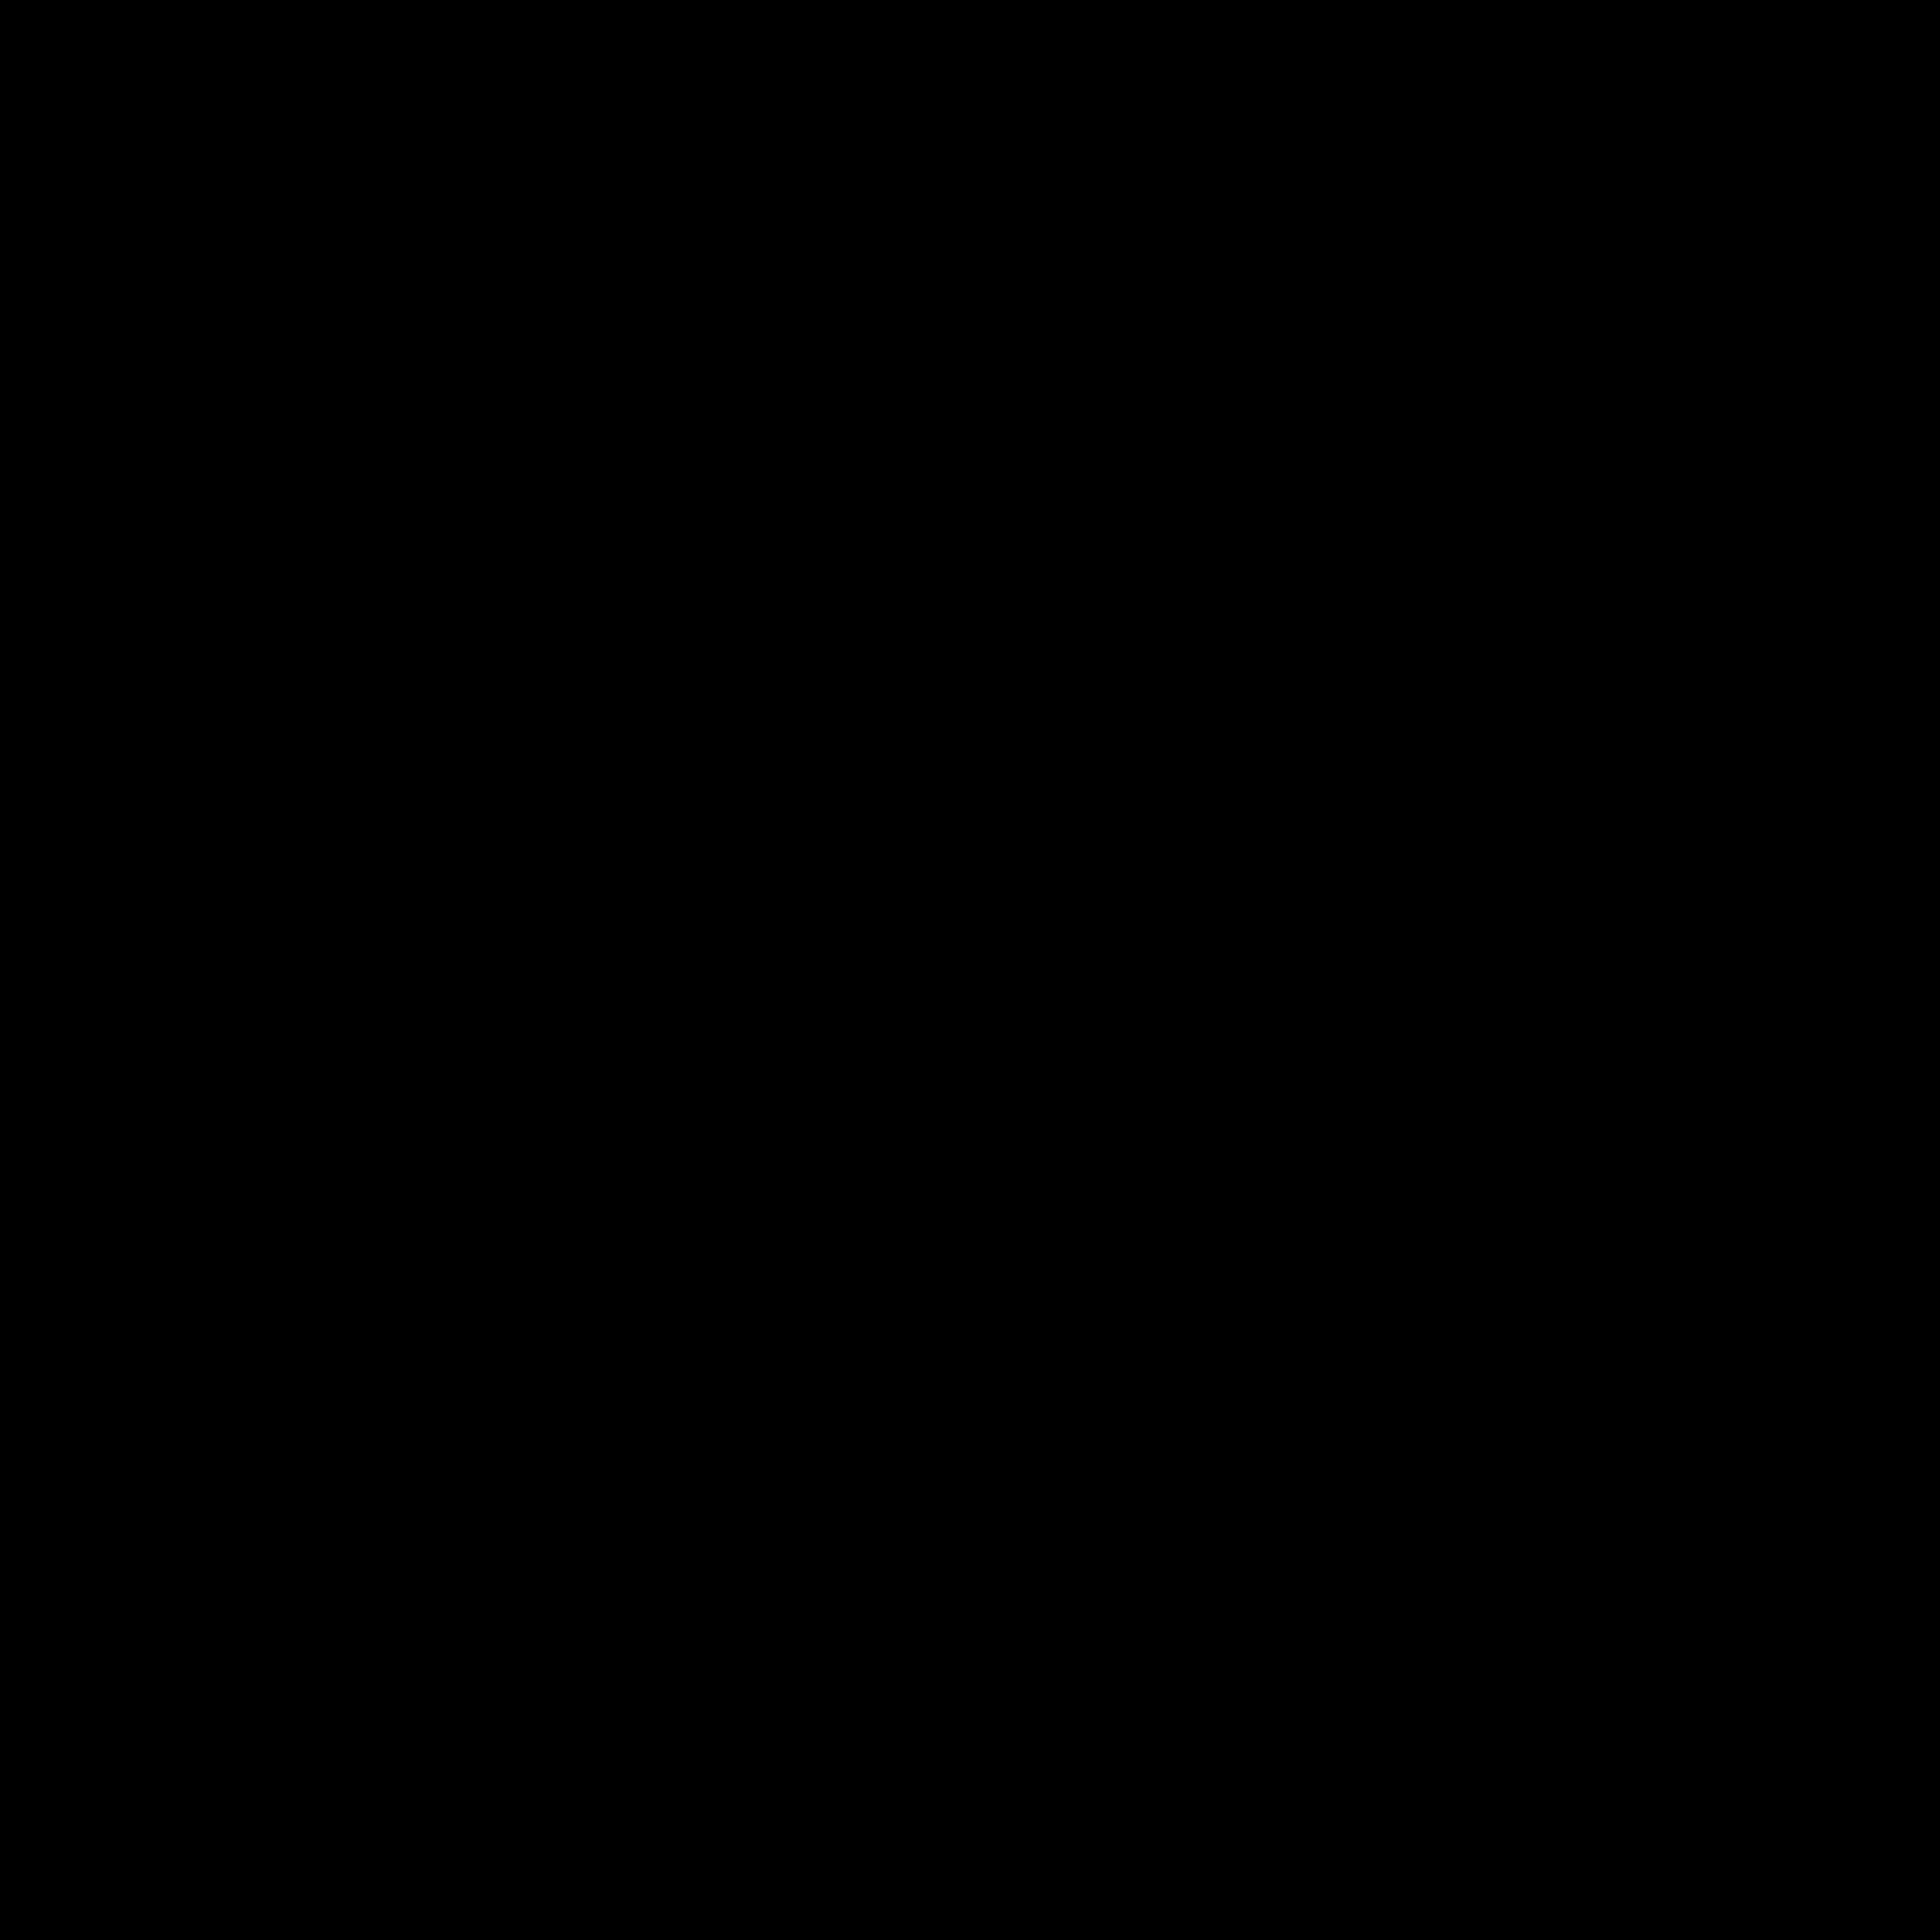
\includegraphics[width=\linewidth]{images/dense}
\caption{dense}
\end{subfigure}~%
\begin{subfigure}{\linewidth}
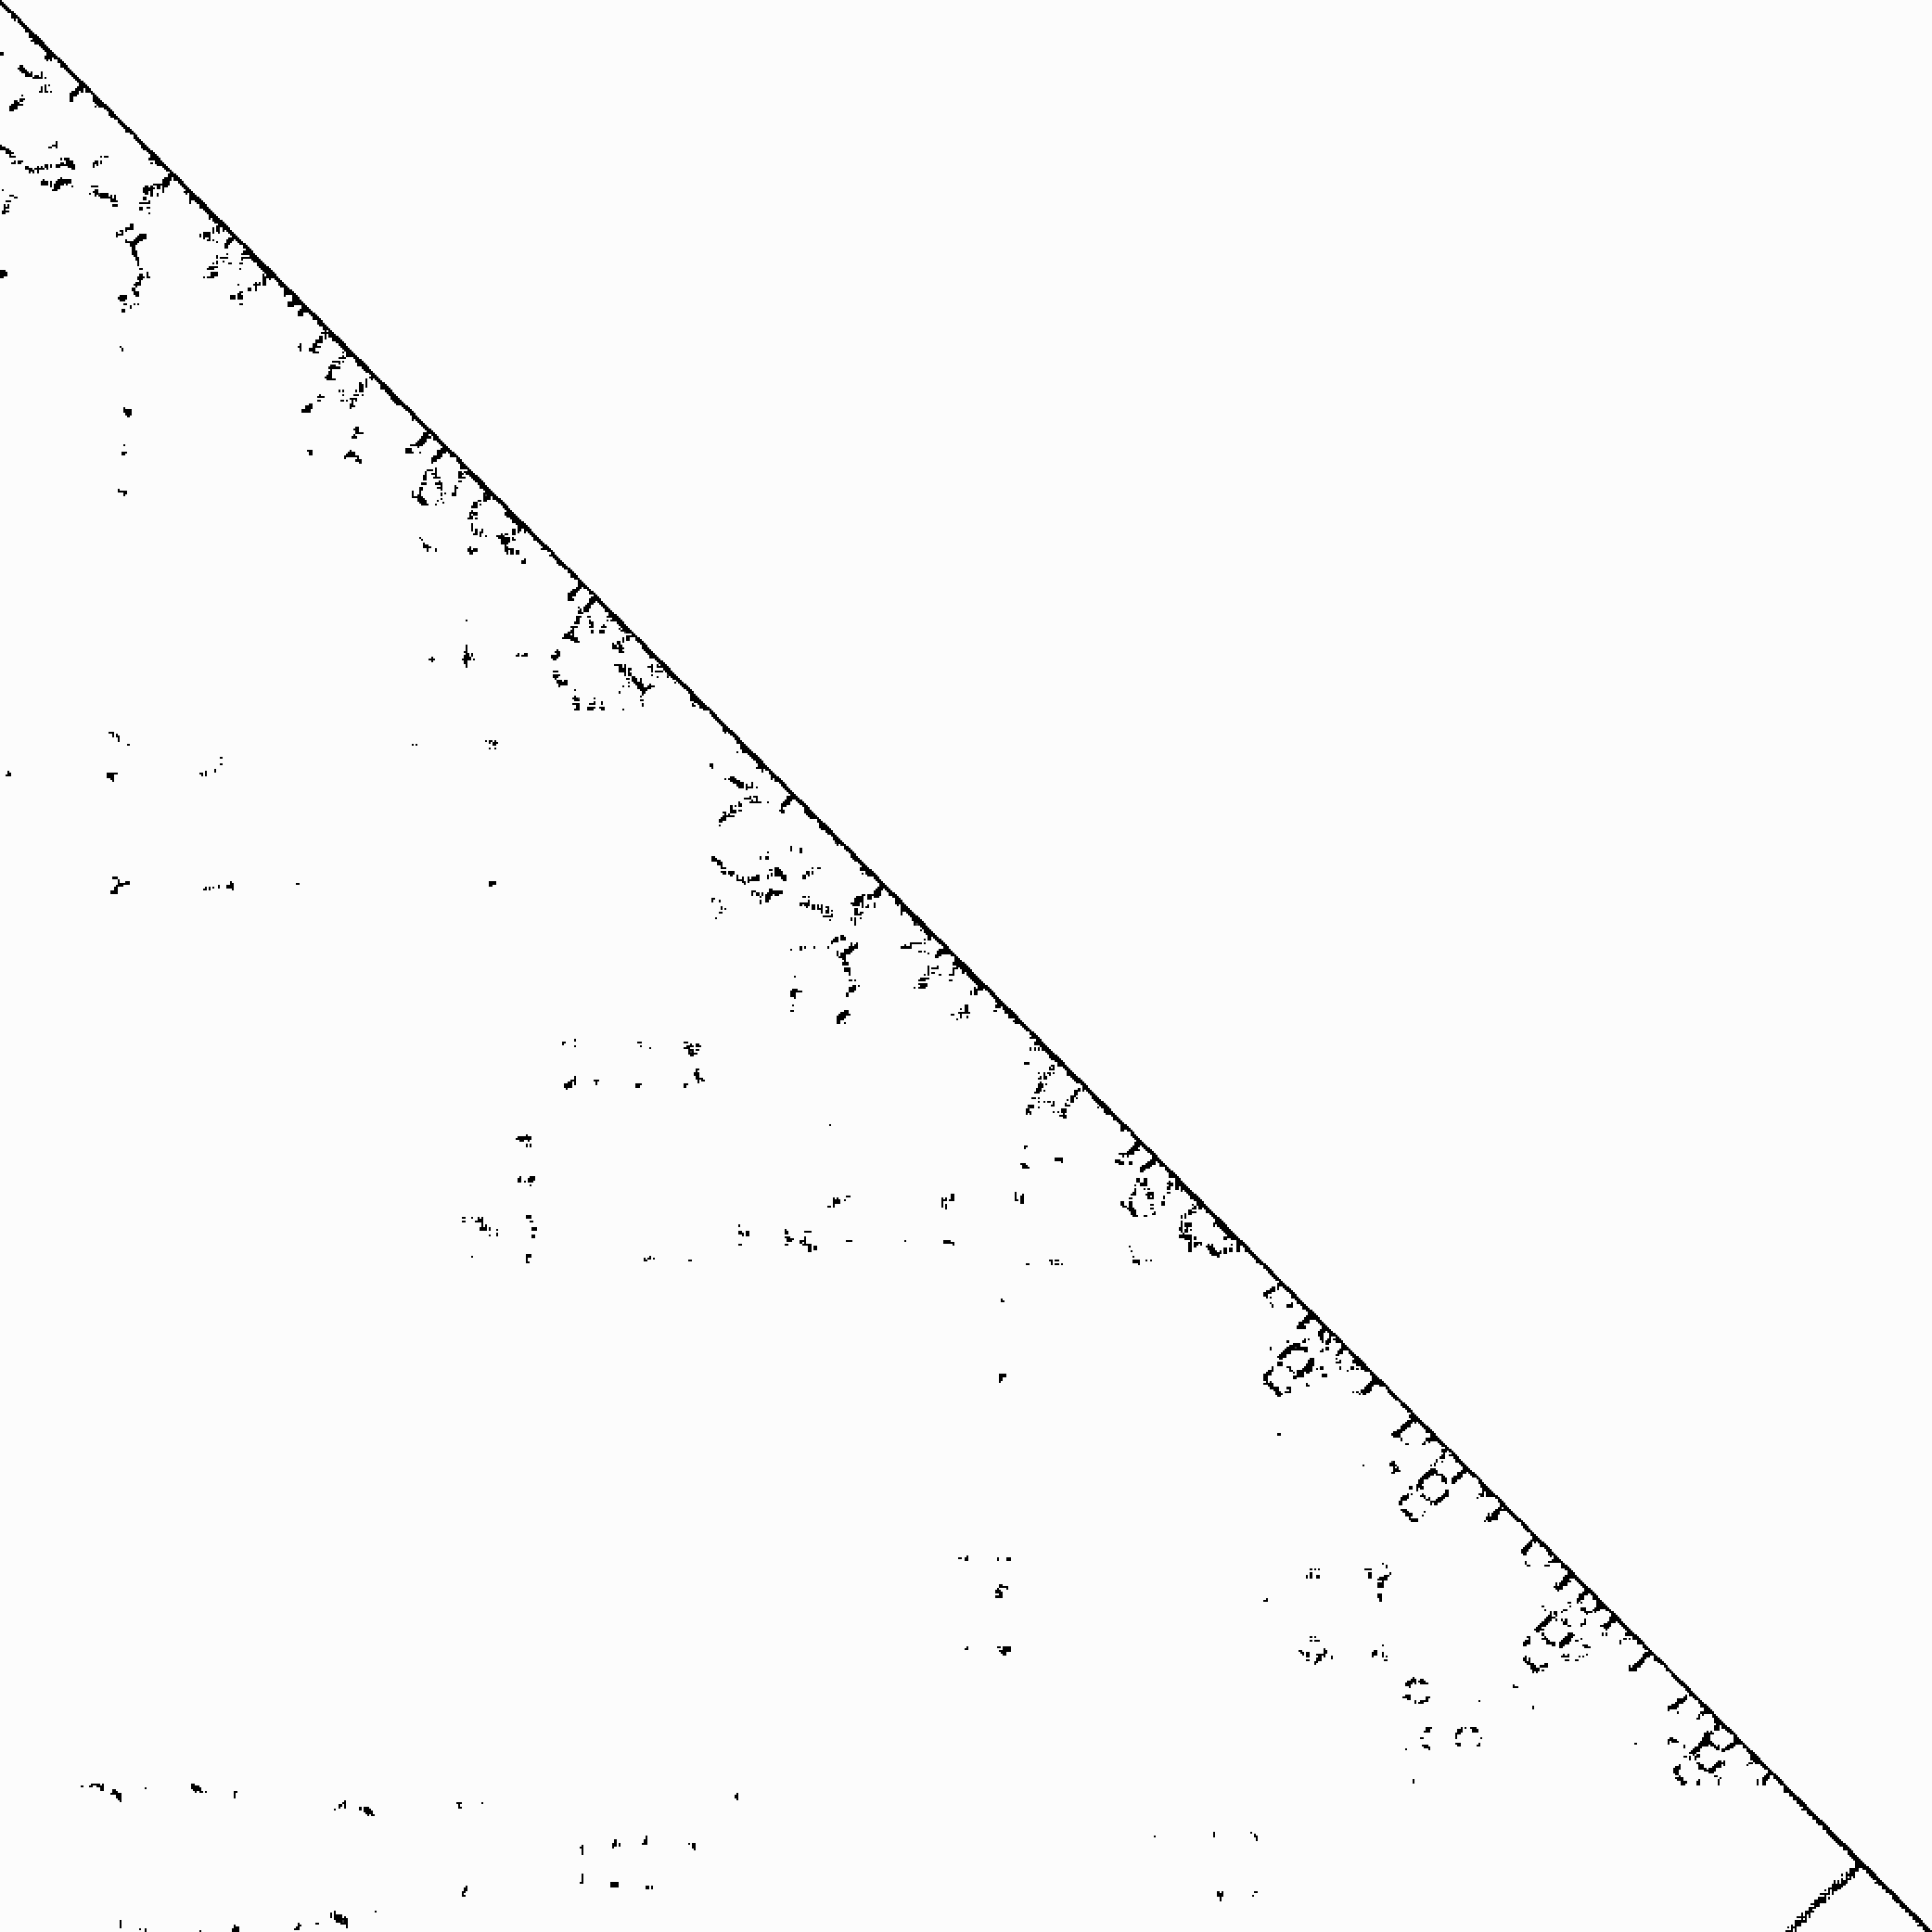
\includegraphics[width=\linewidth]{images/pdb1HYS}
\caption{pdb1HYS}
\end{subfigure}~%
\begin{subfigure}{\linewidth}
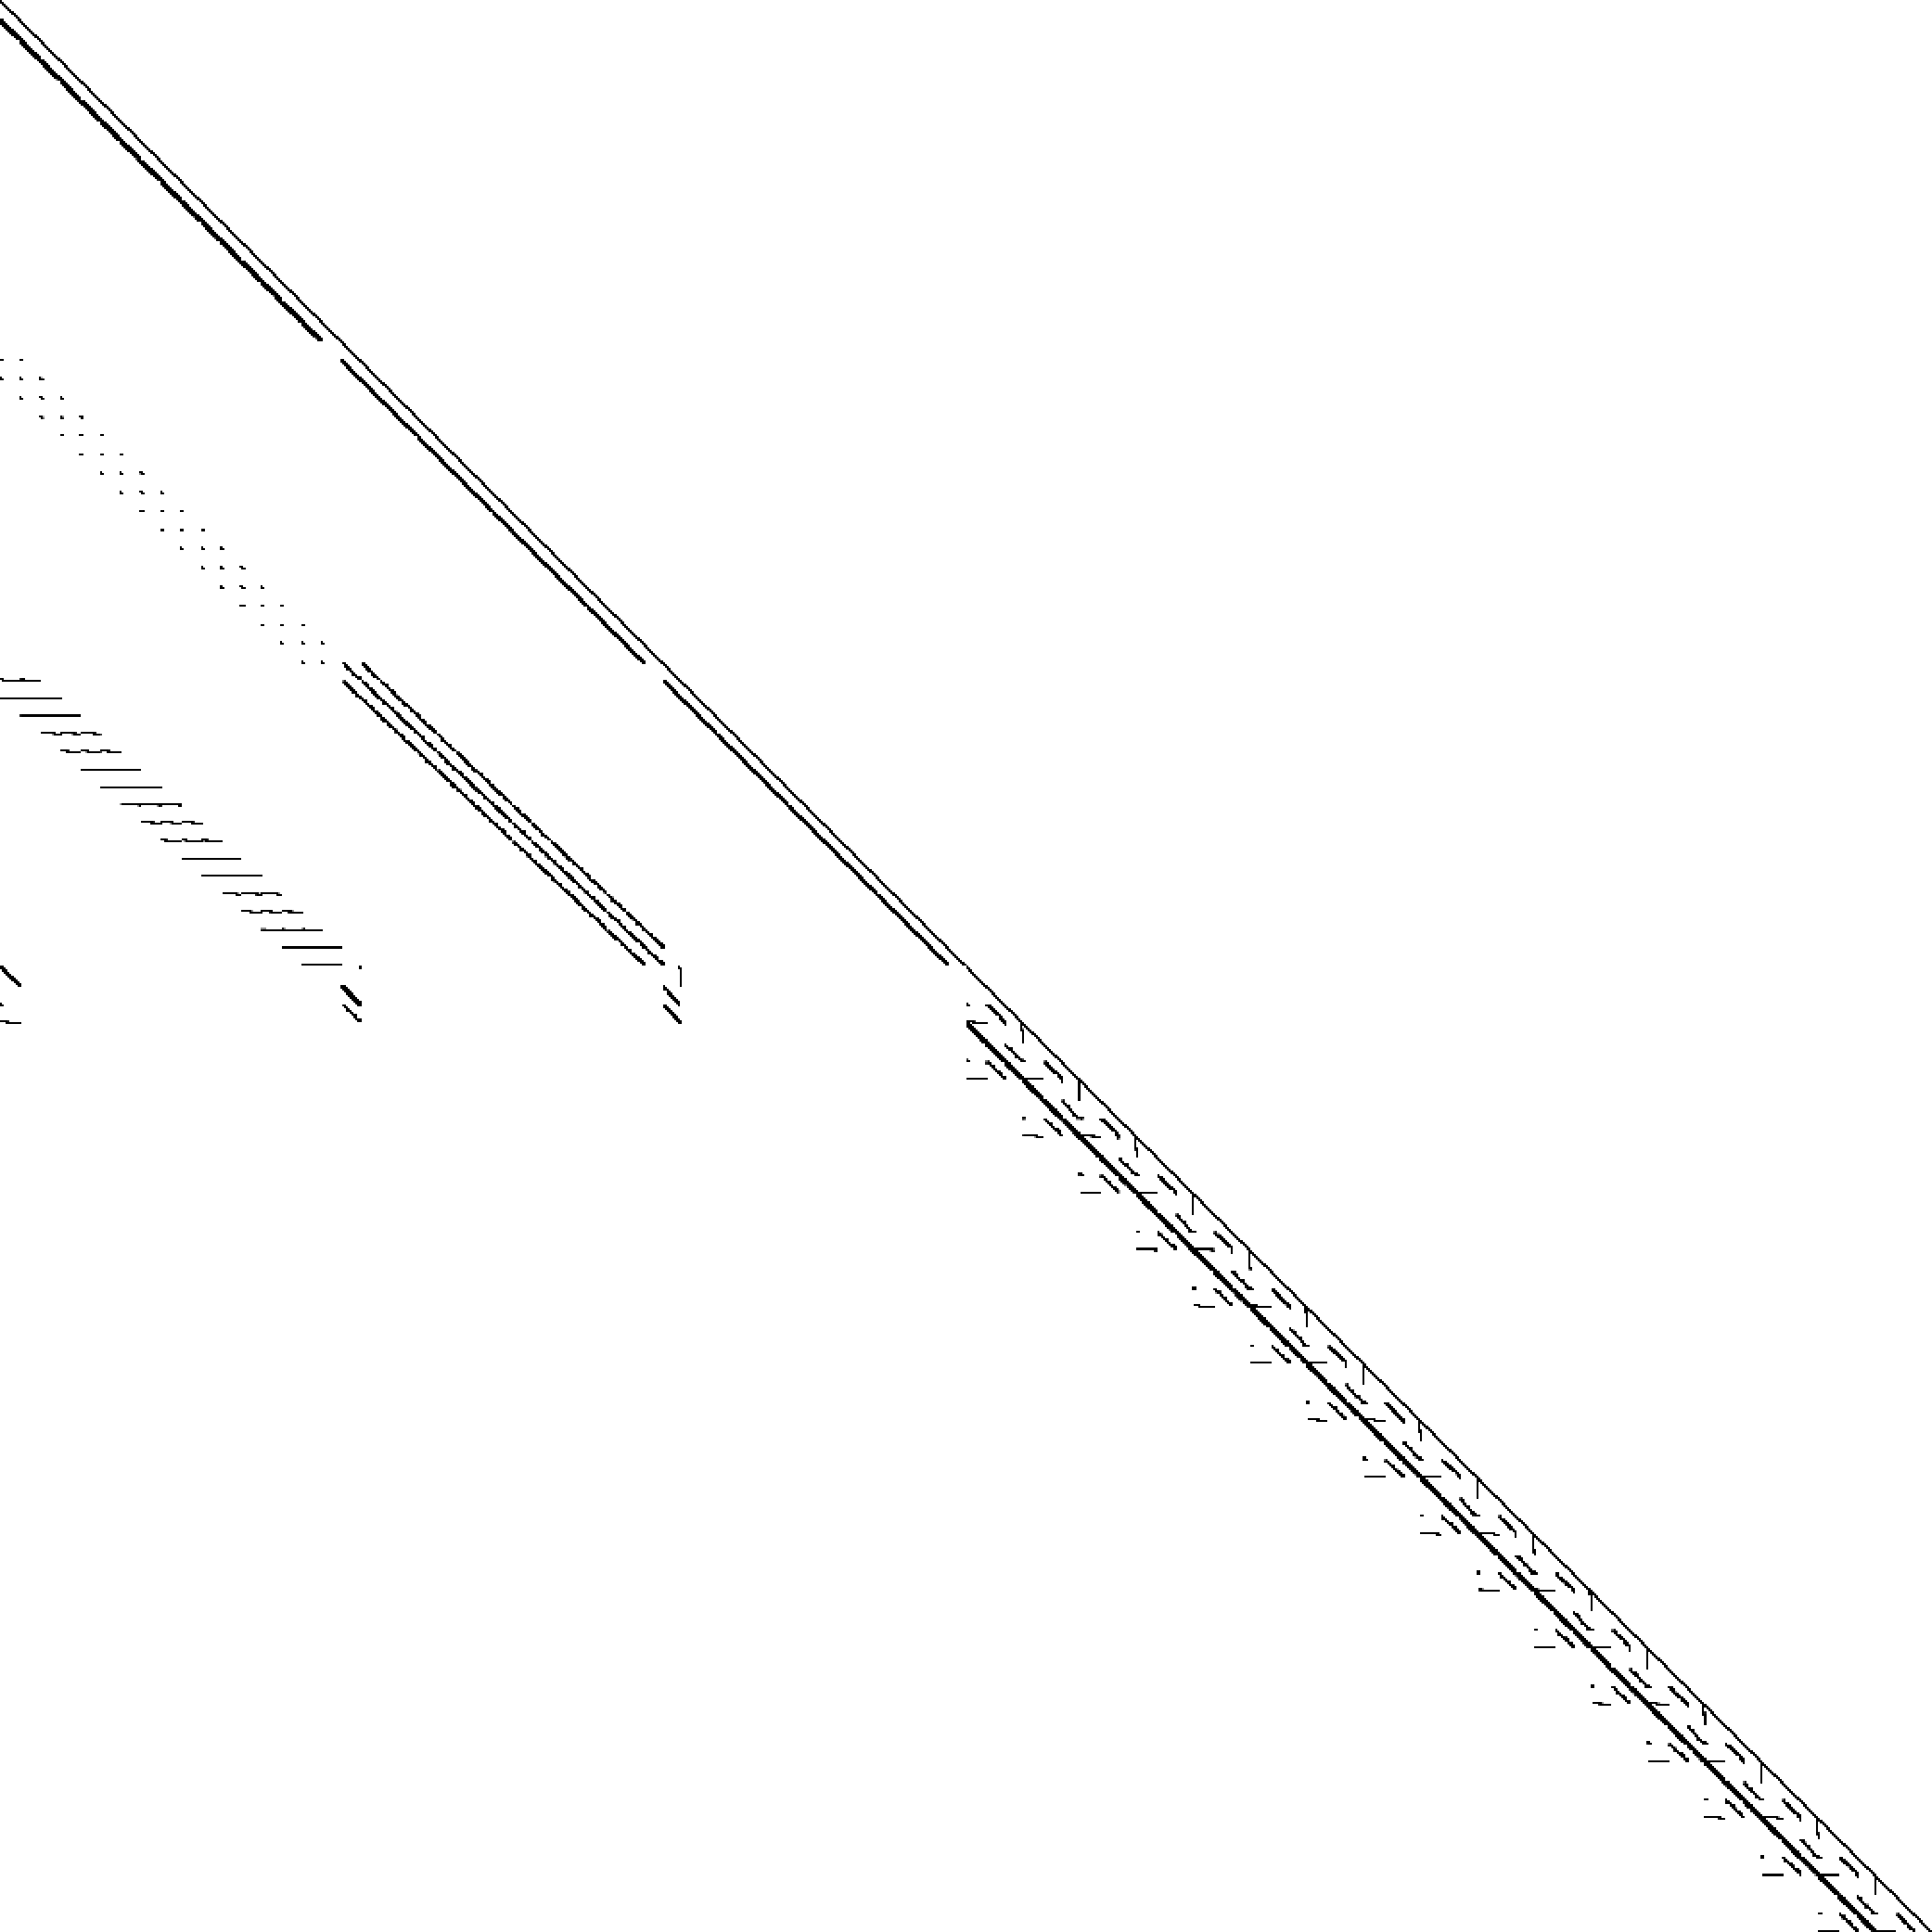
\includegraphics[width=\linewidth]{images/consph}
\caption{consph}
\end{subfigure}~%
\end{multicols}
%\begin{multicols}{3}
%\begin{subfigure}{\linewidth}
%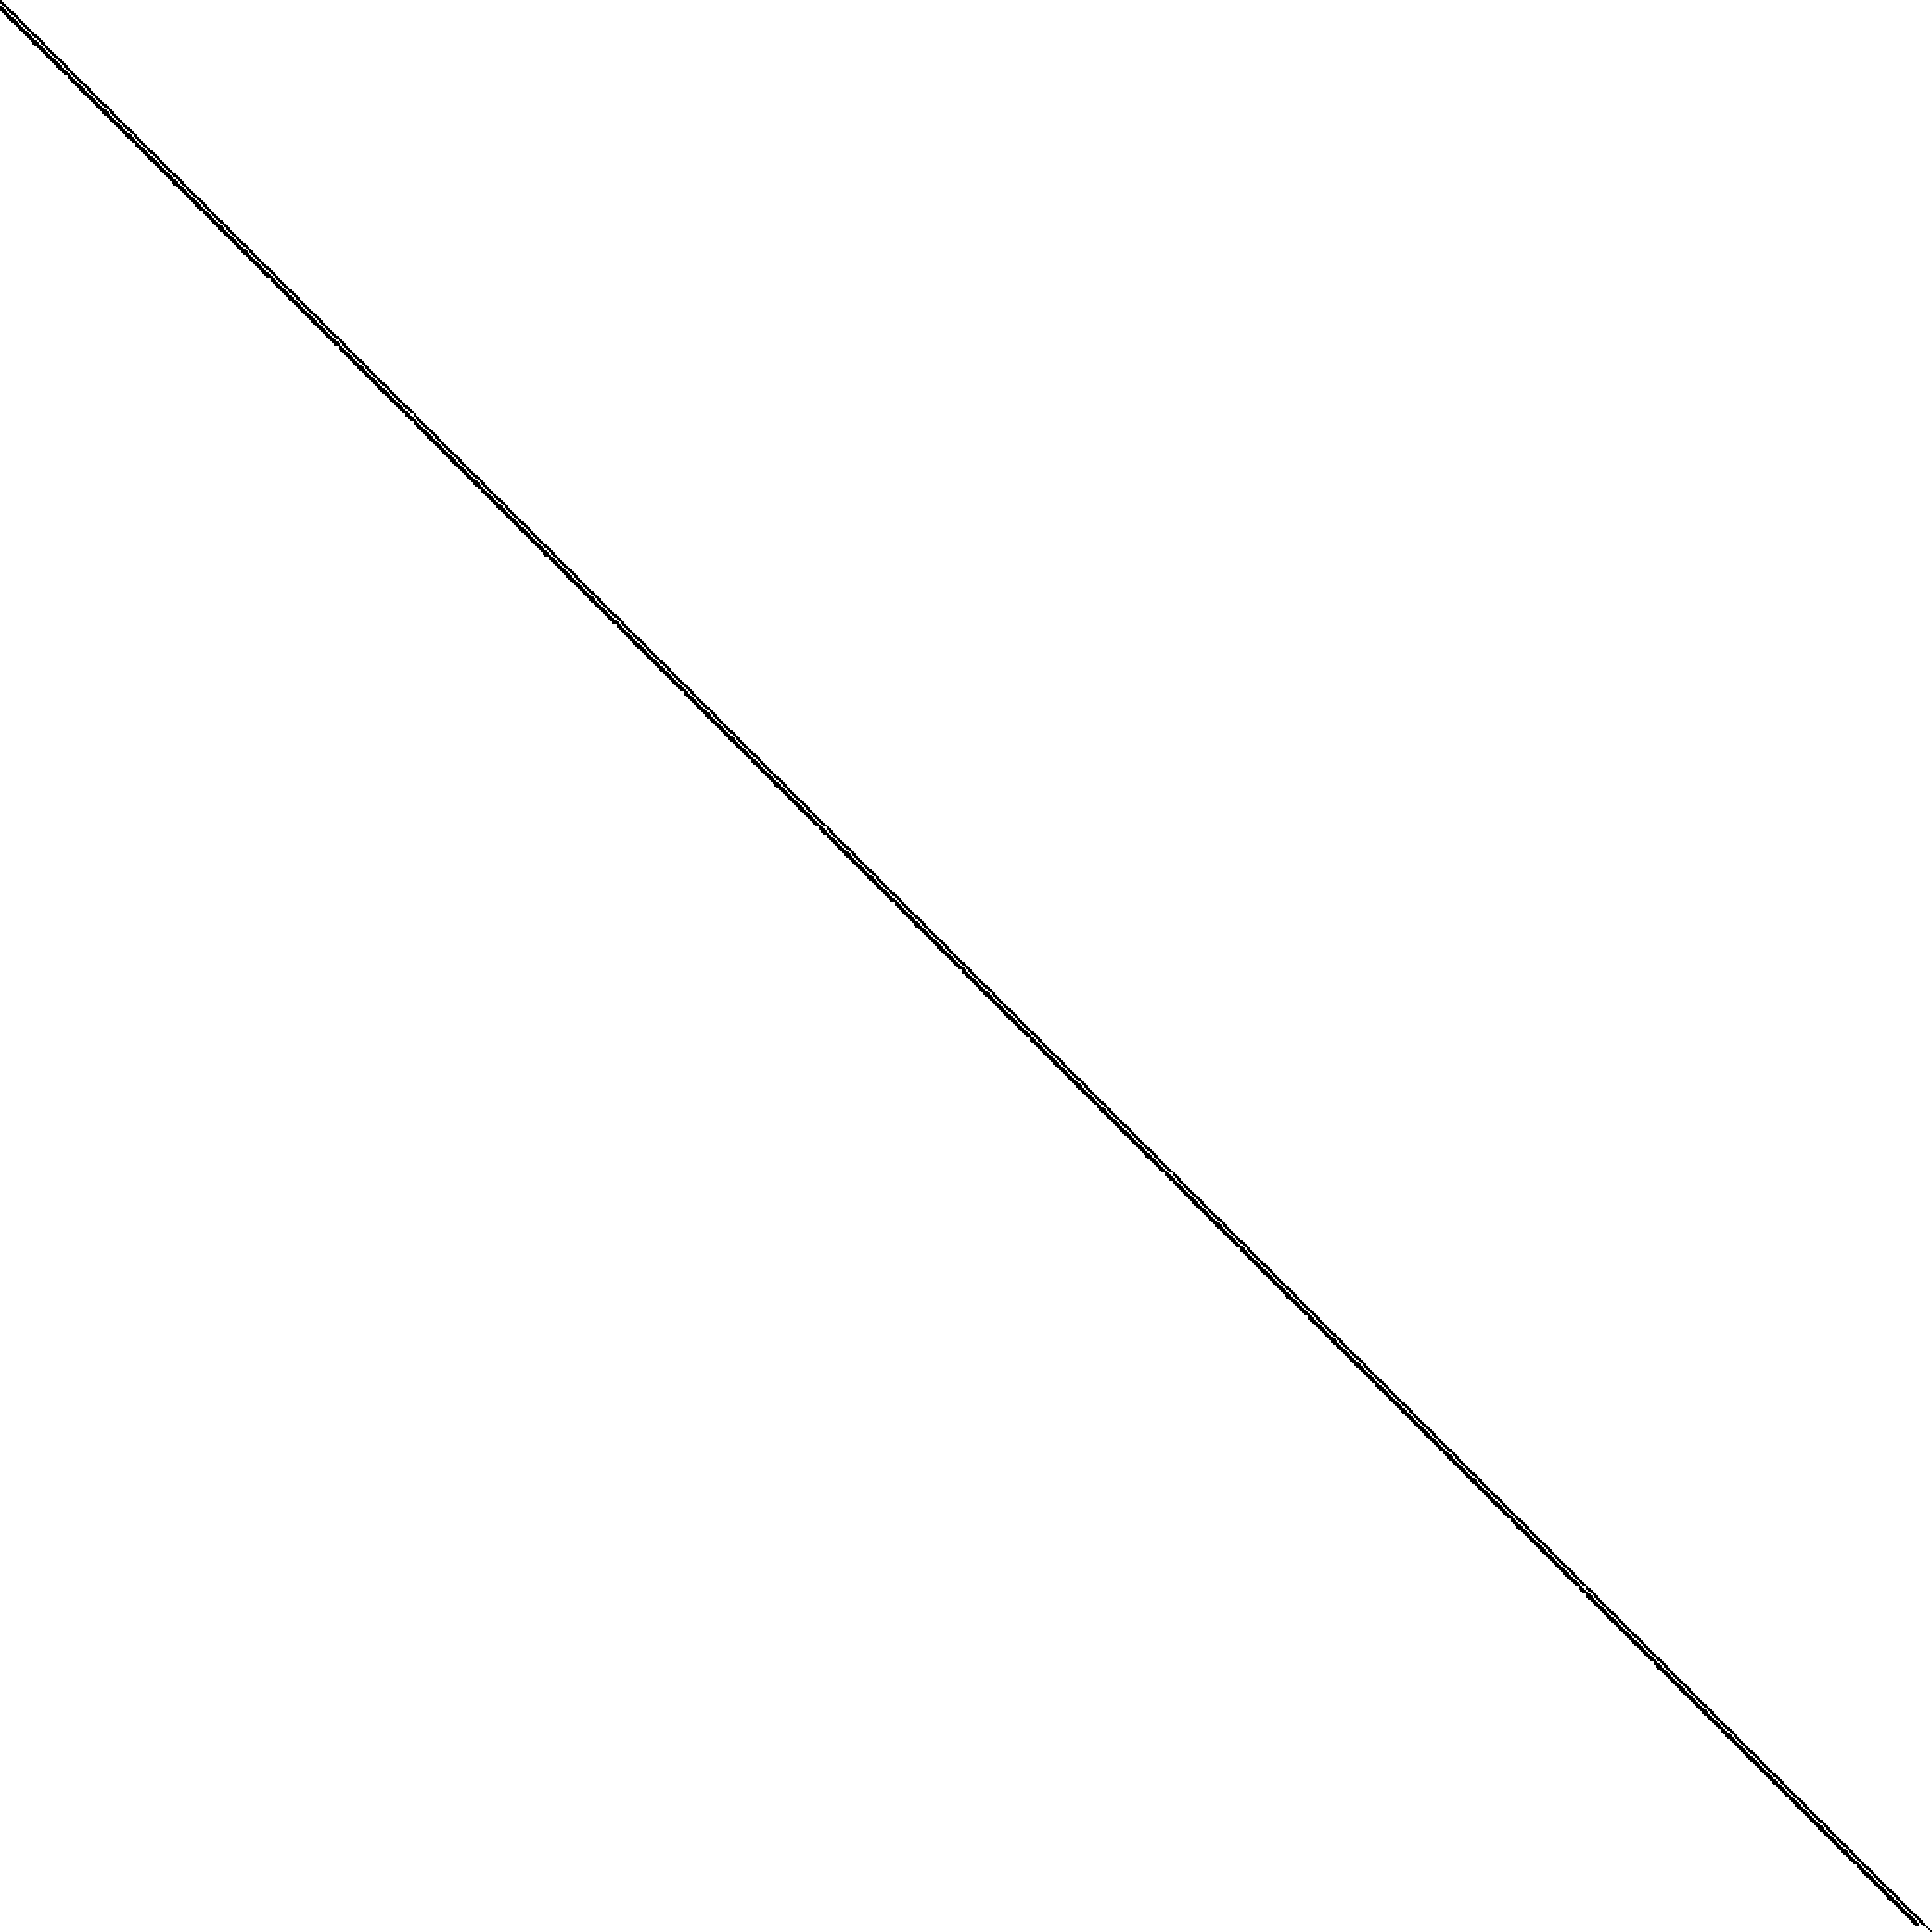
\includegraphics[width=\linewidth]{images/cant}
%\caption{cant}
%\end{subfigure}~%
%\begin{subfigure}{\linewidth}
%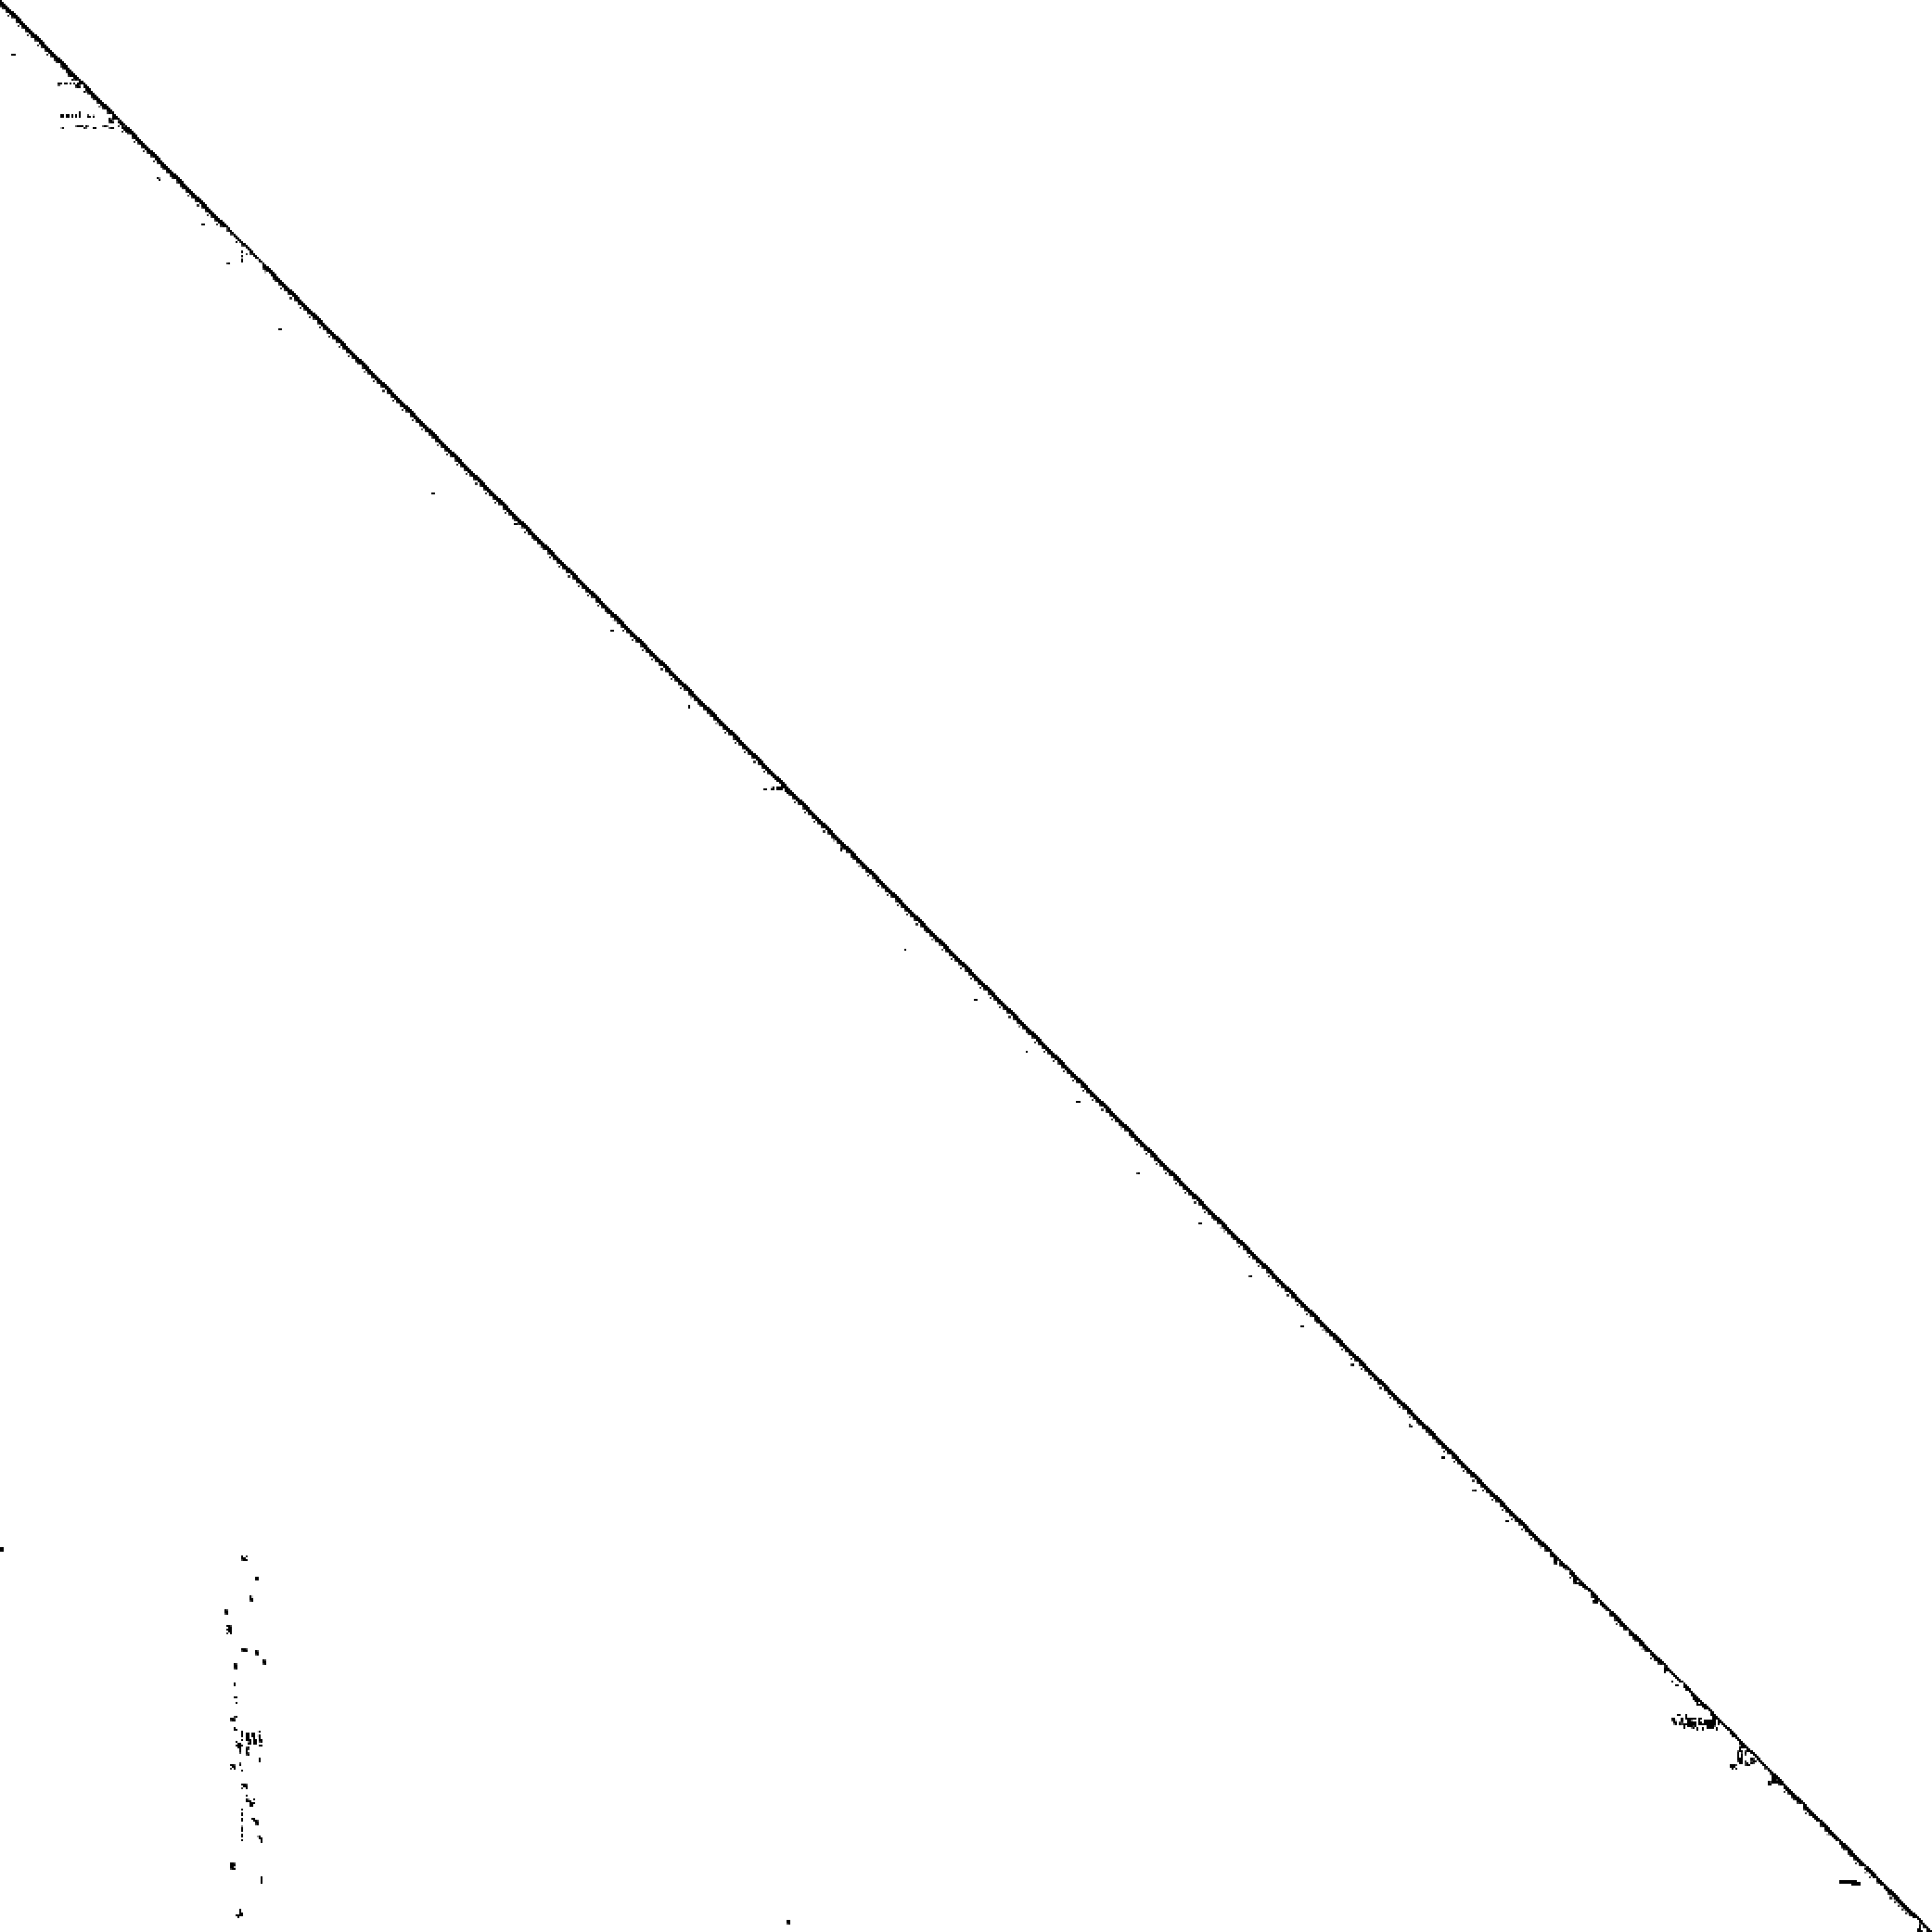
\includegraphics[width=\linewidth]{images/pwtk}
%\caption{pwtk}
%\end{subfigure}~%
%\begin{subfigure}{\linewidth}
%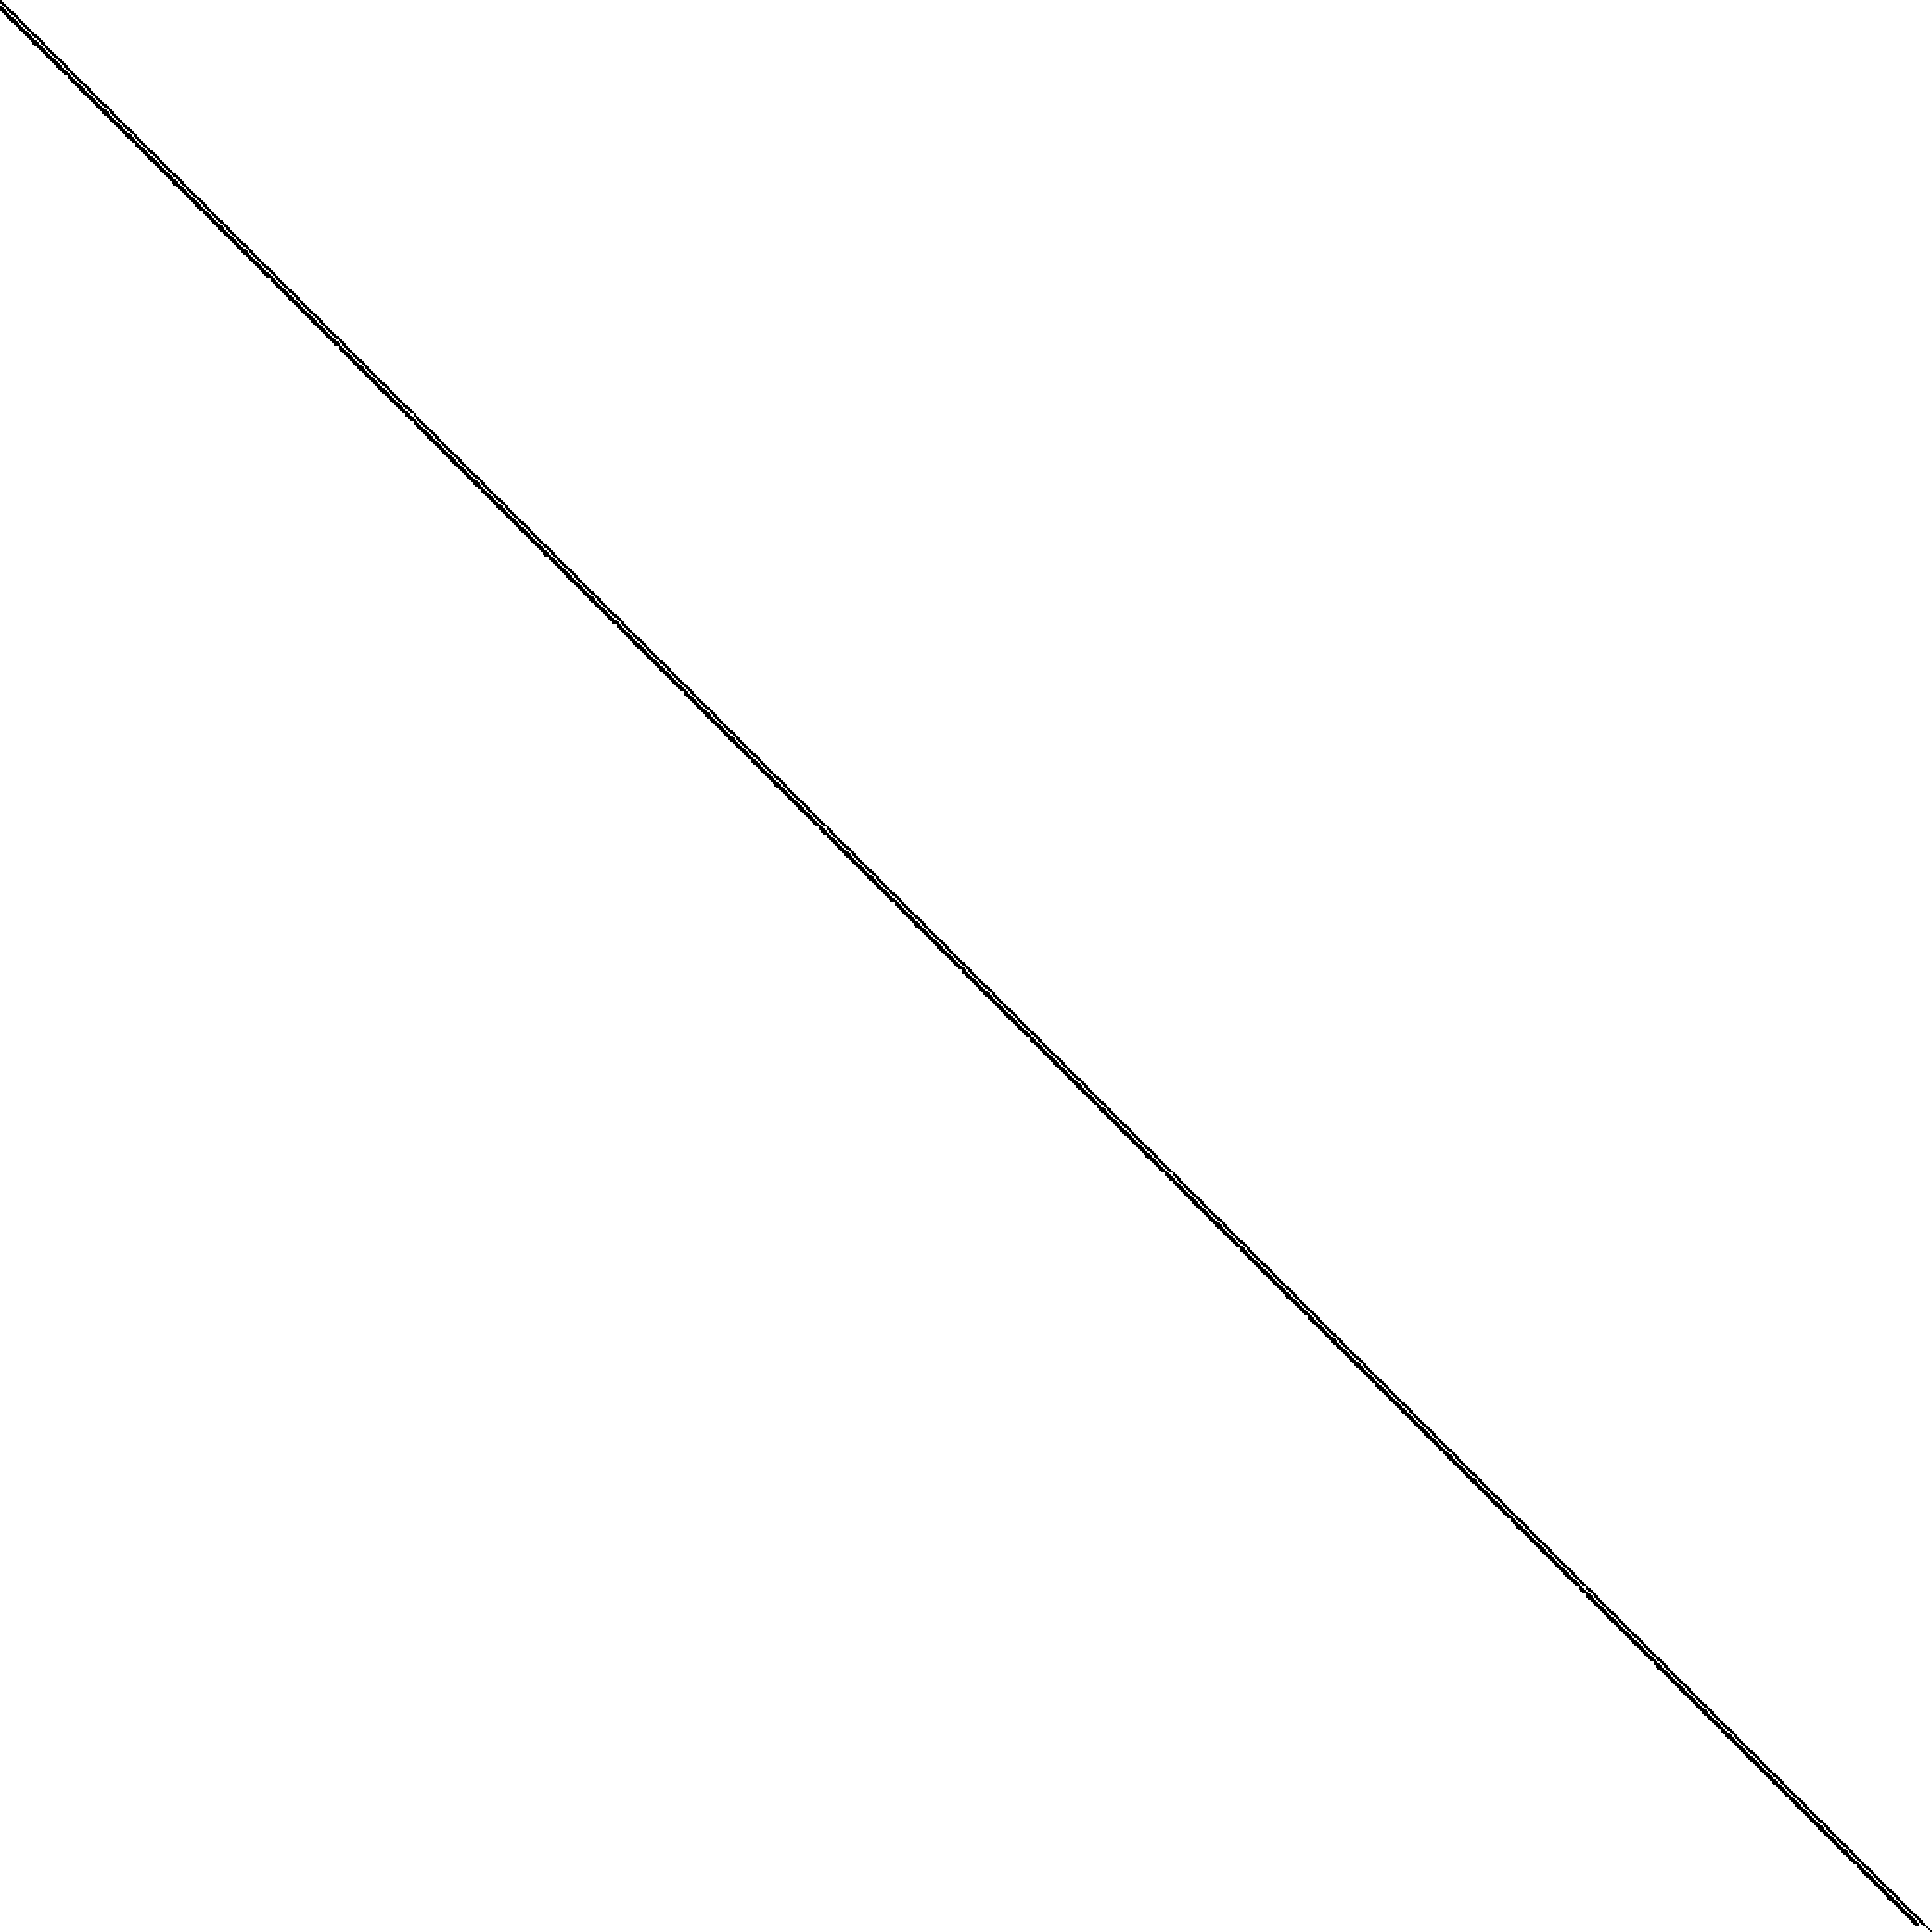
\includegraphics[width=\linewidth]{images/cant}
%\caption{cant}
%\end{subfigure}~%
%\end{multicols}
\begin{multicols}{3}
\begin{subfigure}{\linewidth}
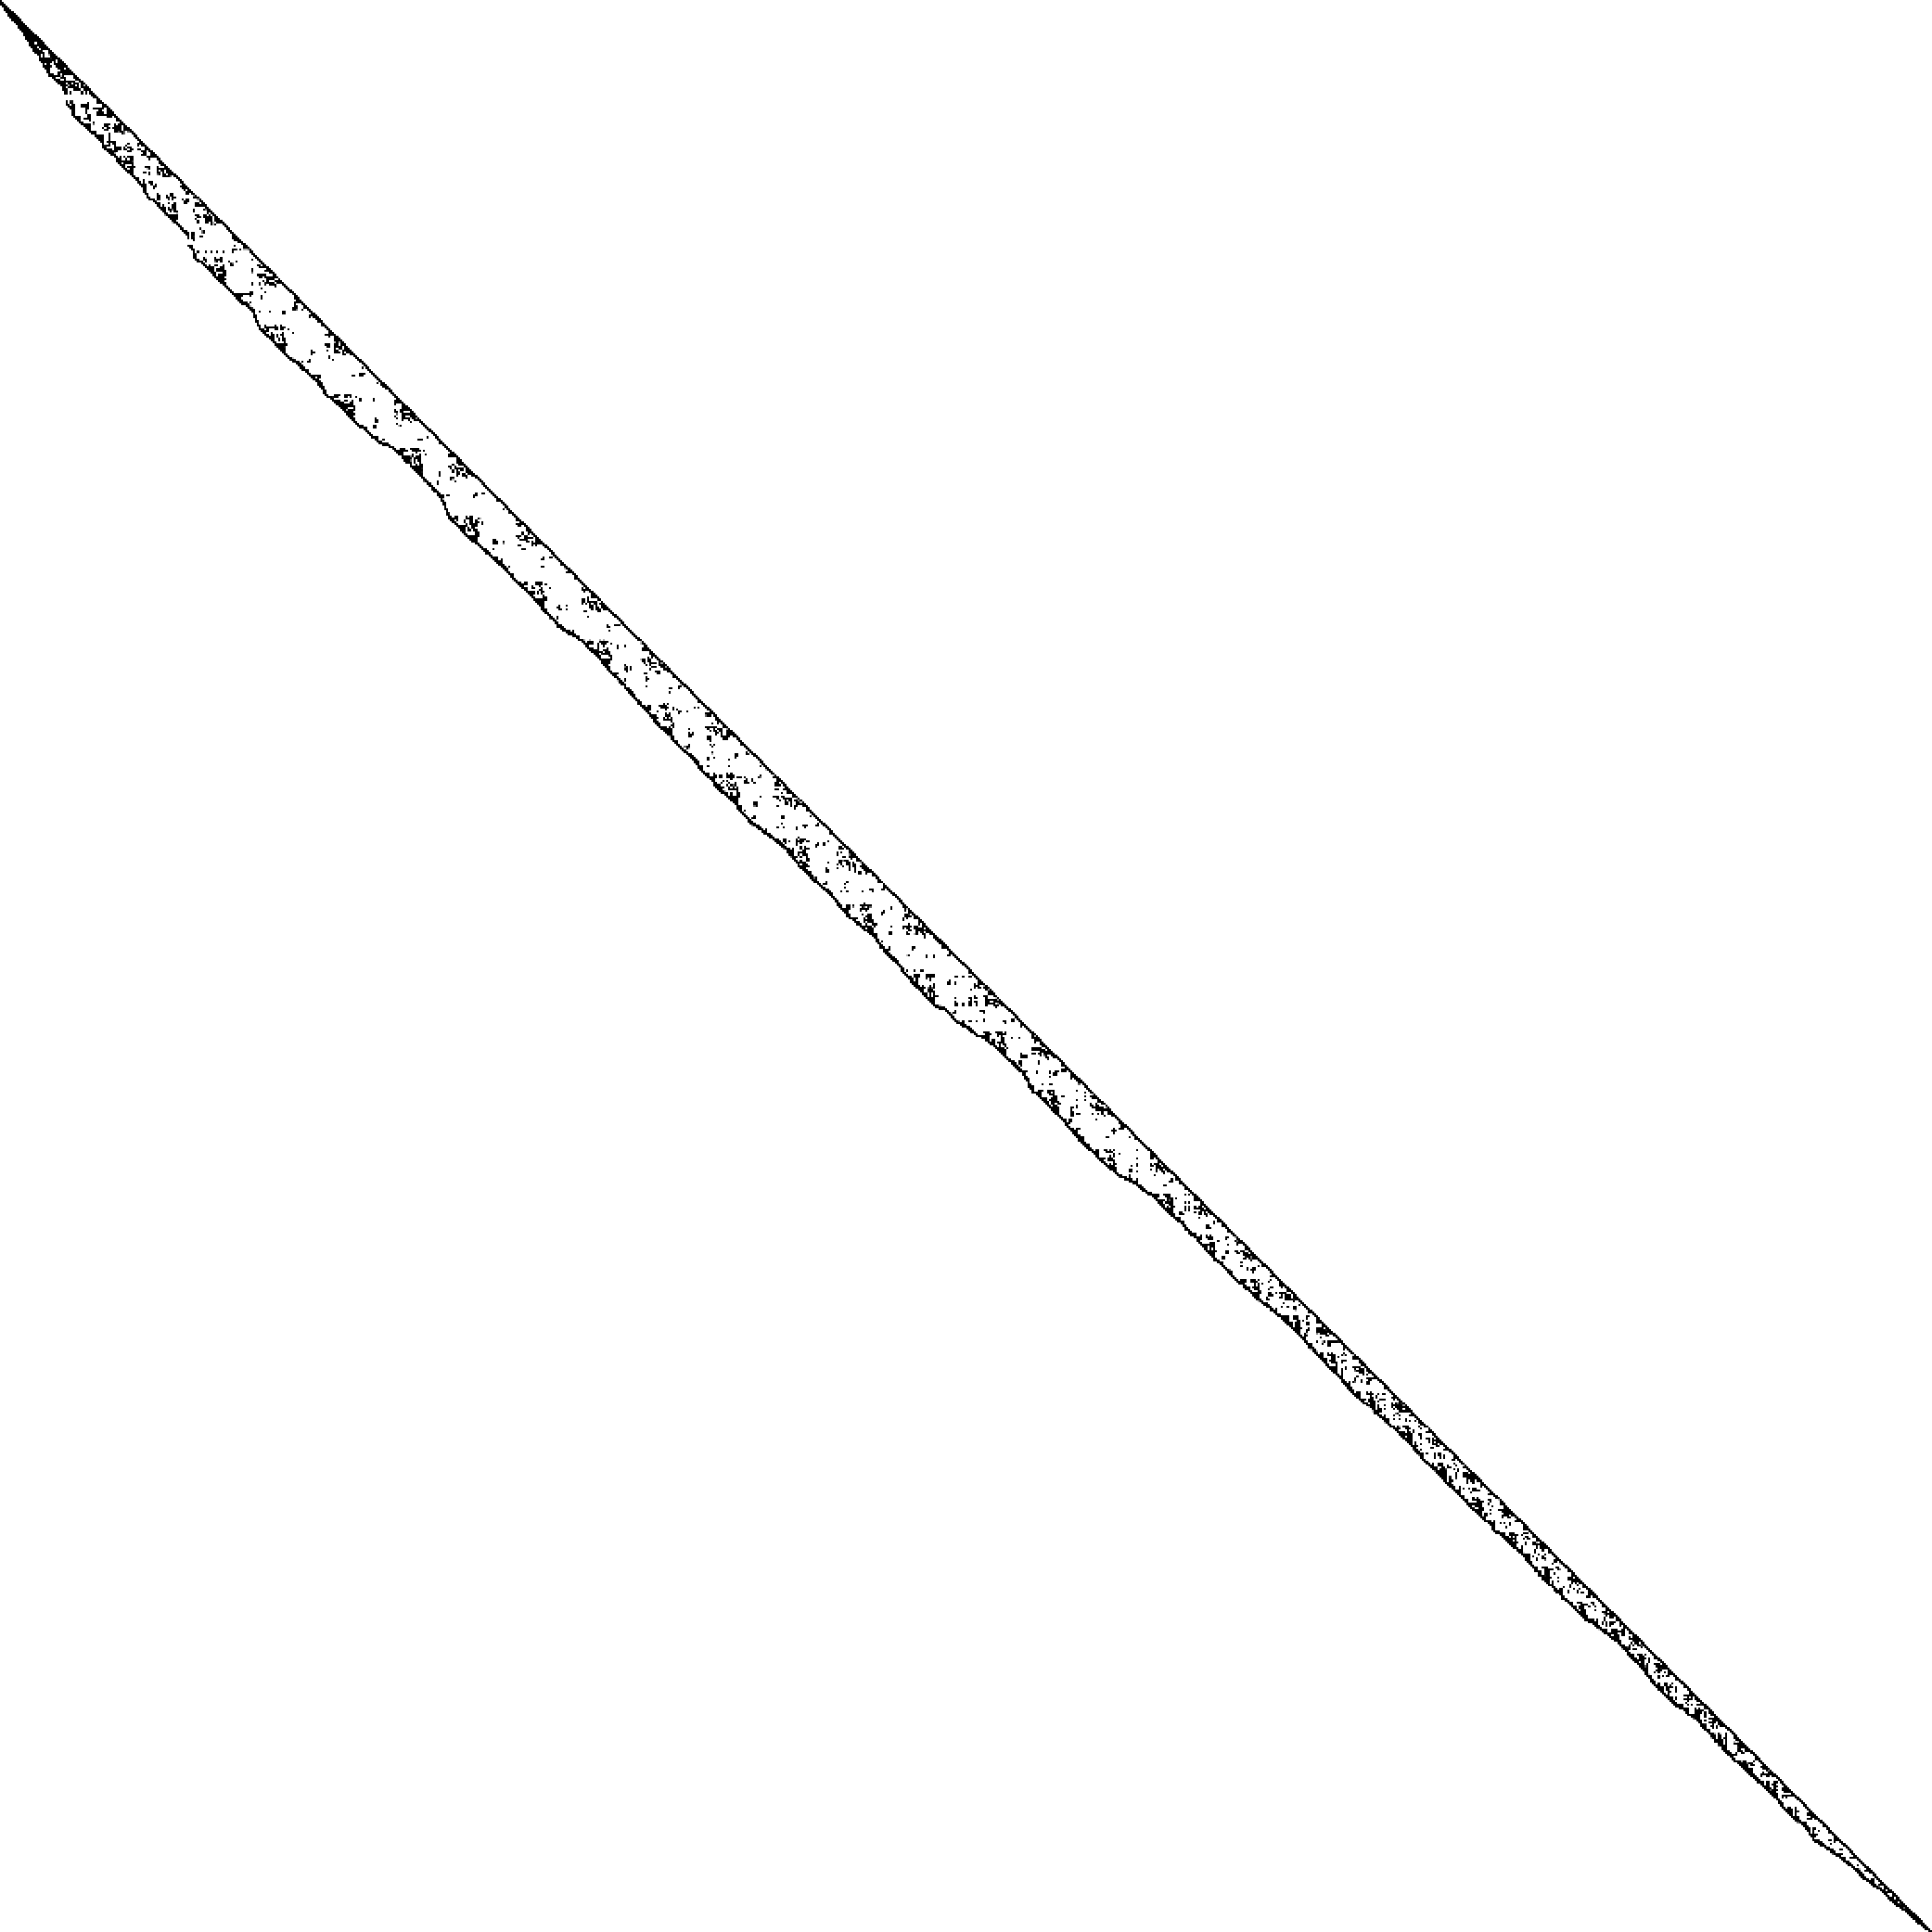
\includegraphics[width=\linewidth]{images/shipsec1}
\caption{shipsec1}
\end{subfigure}~%
\begin{subfigure}{\linewidth}
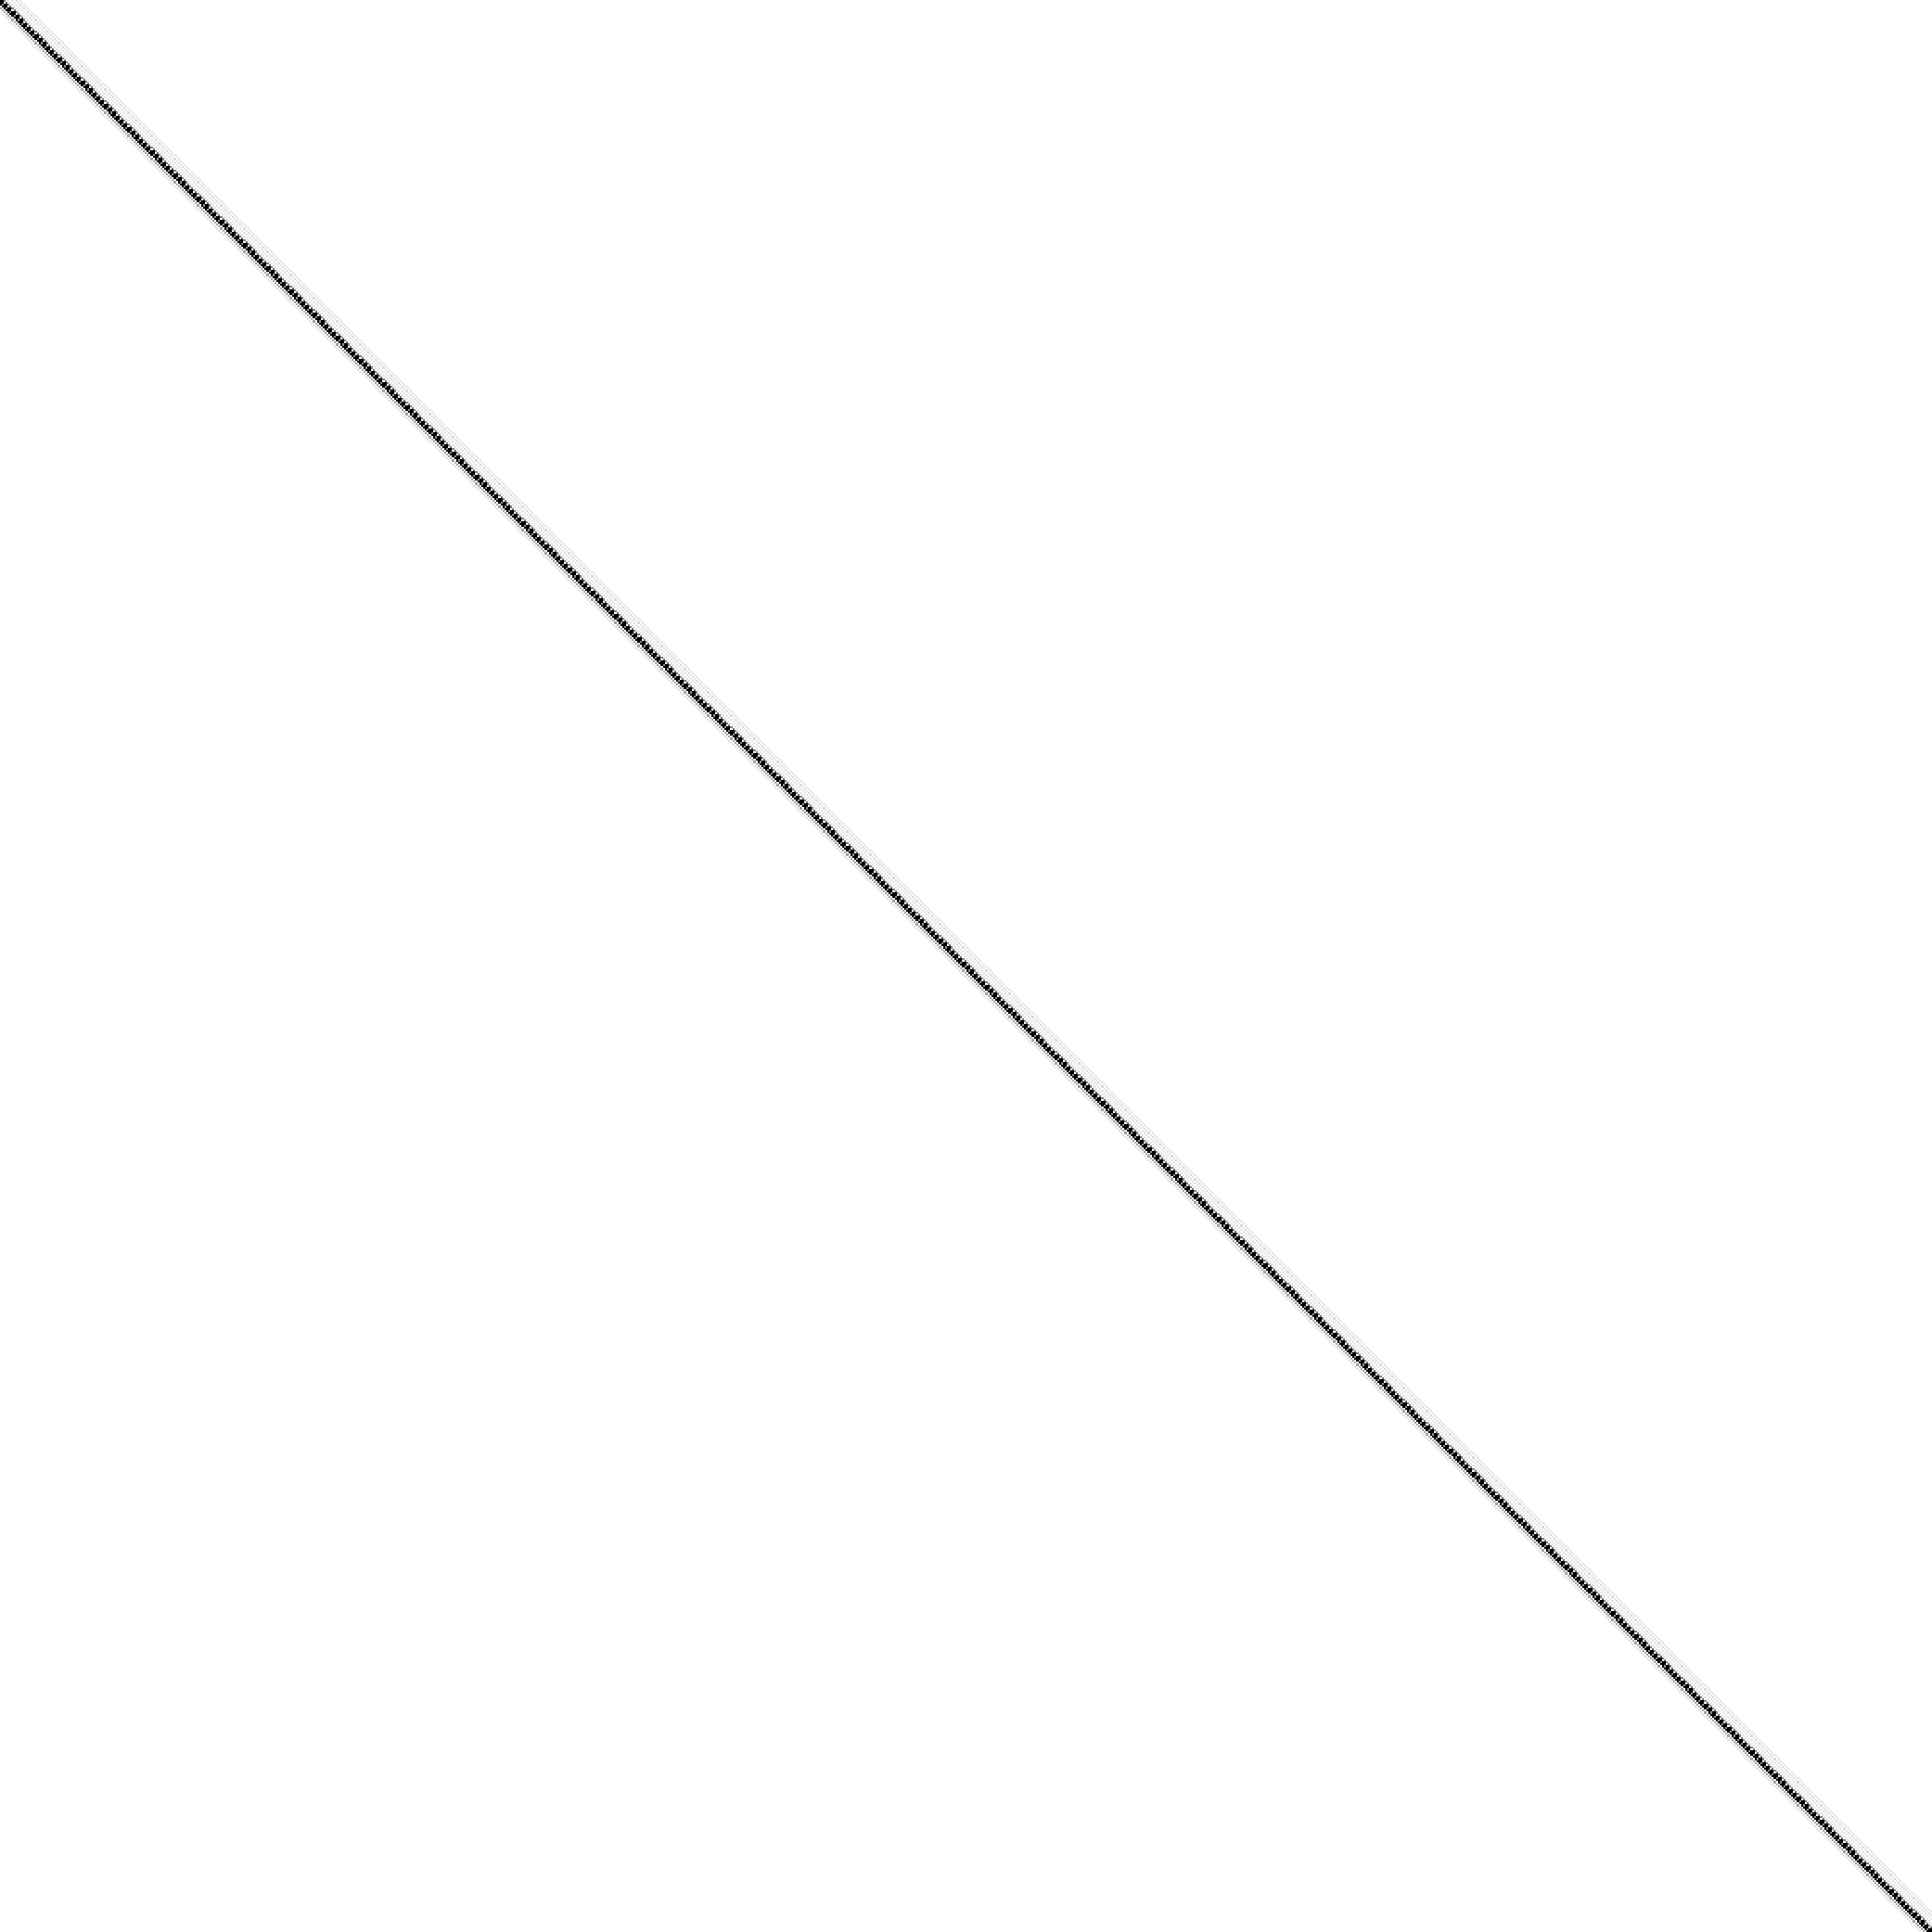
\includegraphics[width=\linewidth]{images/mac_econ_fwd500}
\caption{mac\_econ\_fwd500}
\end{subfigure}~%
\begin{subfigure}{\linewidth}
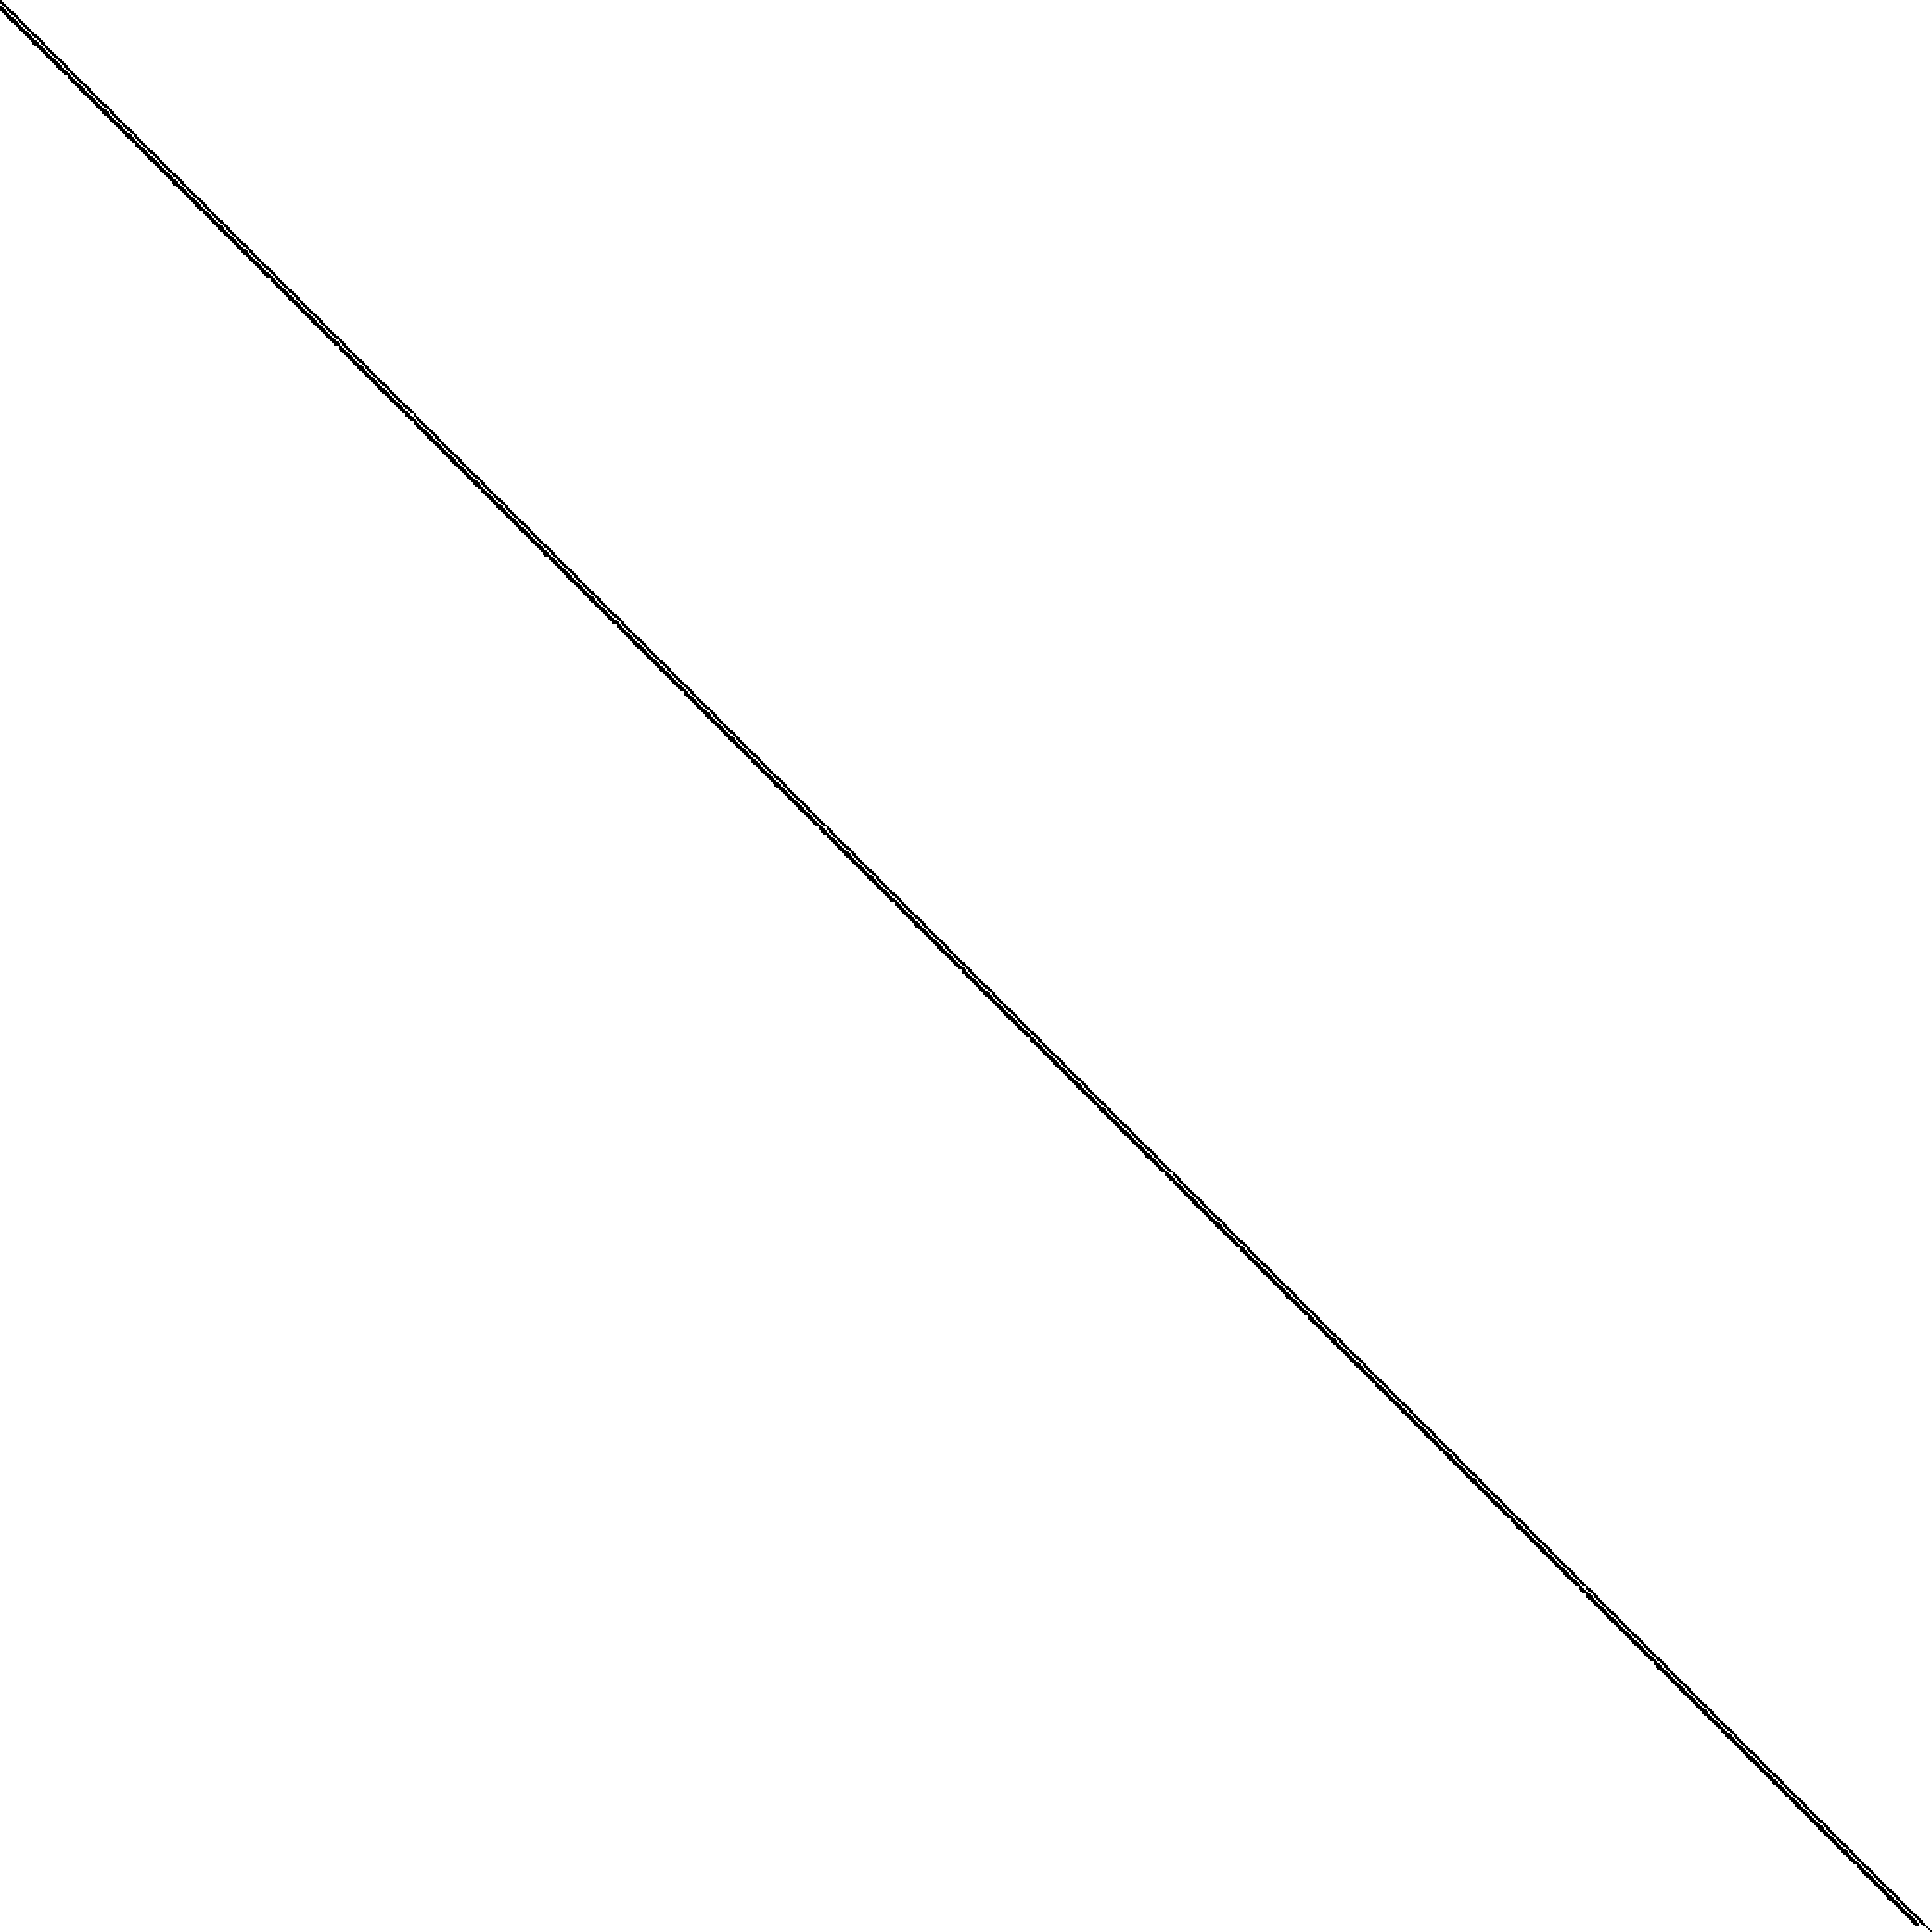
\includegraphics[width=\linewidth]{images/cant}
\caption{cant}
\end{subfigure}~%
\end{multicols}
\begin{multicols}{3}
\begin{subfigure}{\linewidth}

\includegraphics[width=\linewidth]{images/cop20k_A}
\caption{cop20k\_A}
\end{subfigure}~%
\begin{subfigure}{\linewidth}
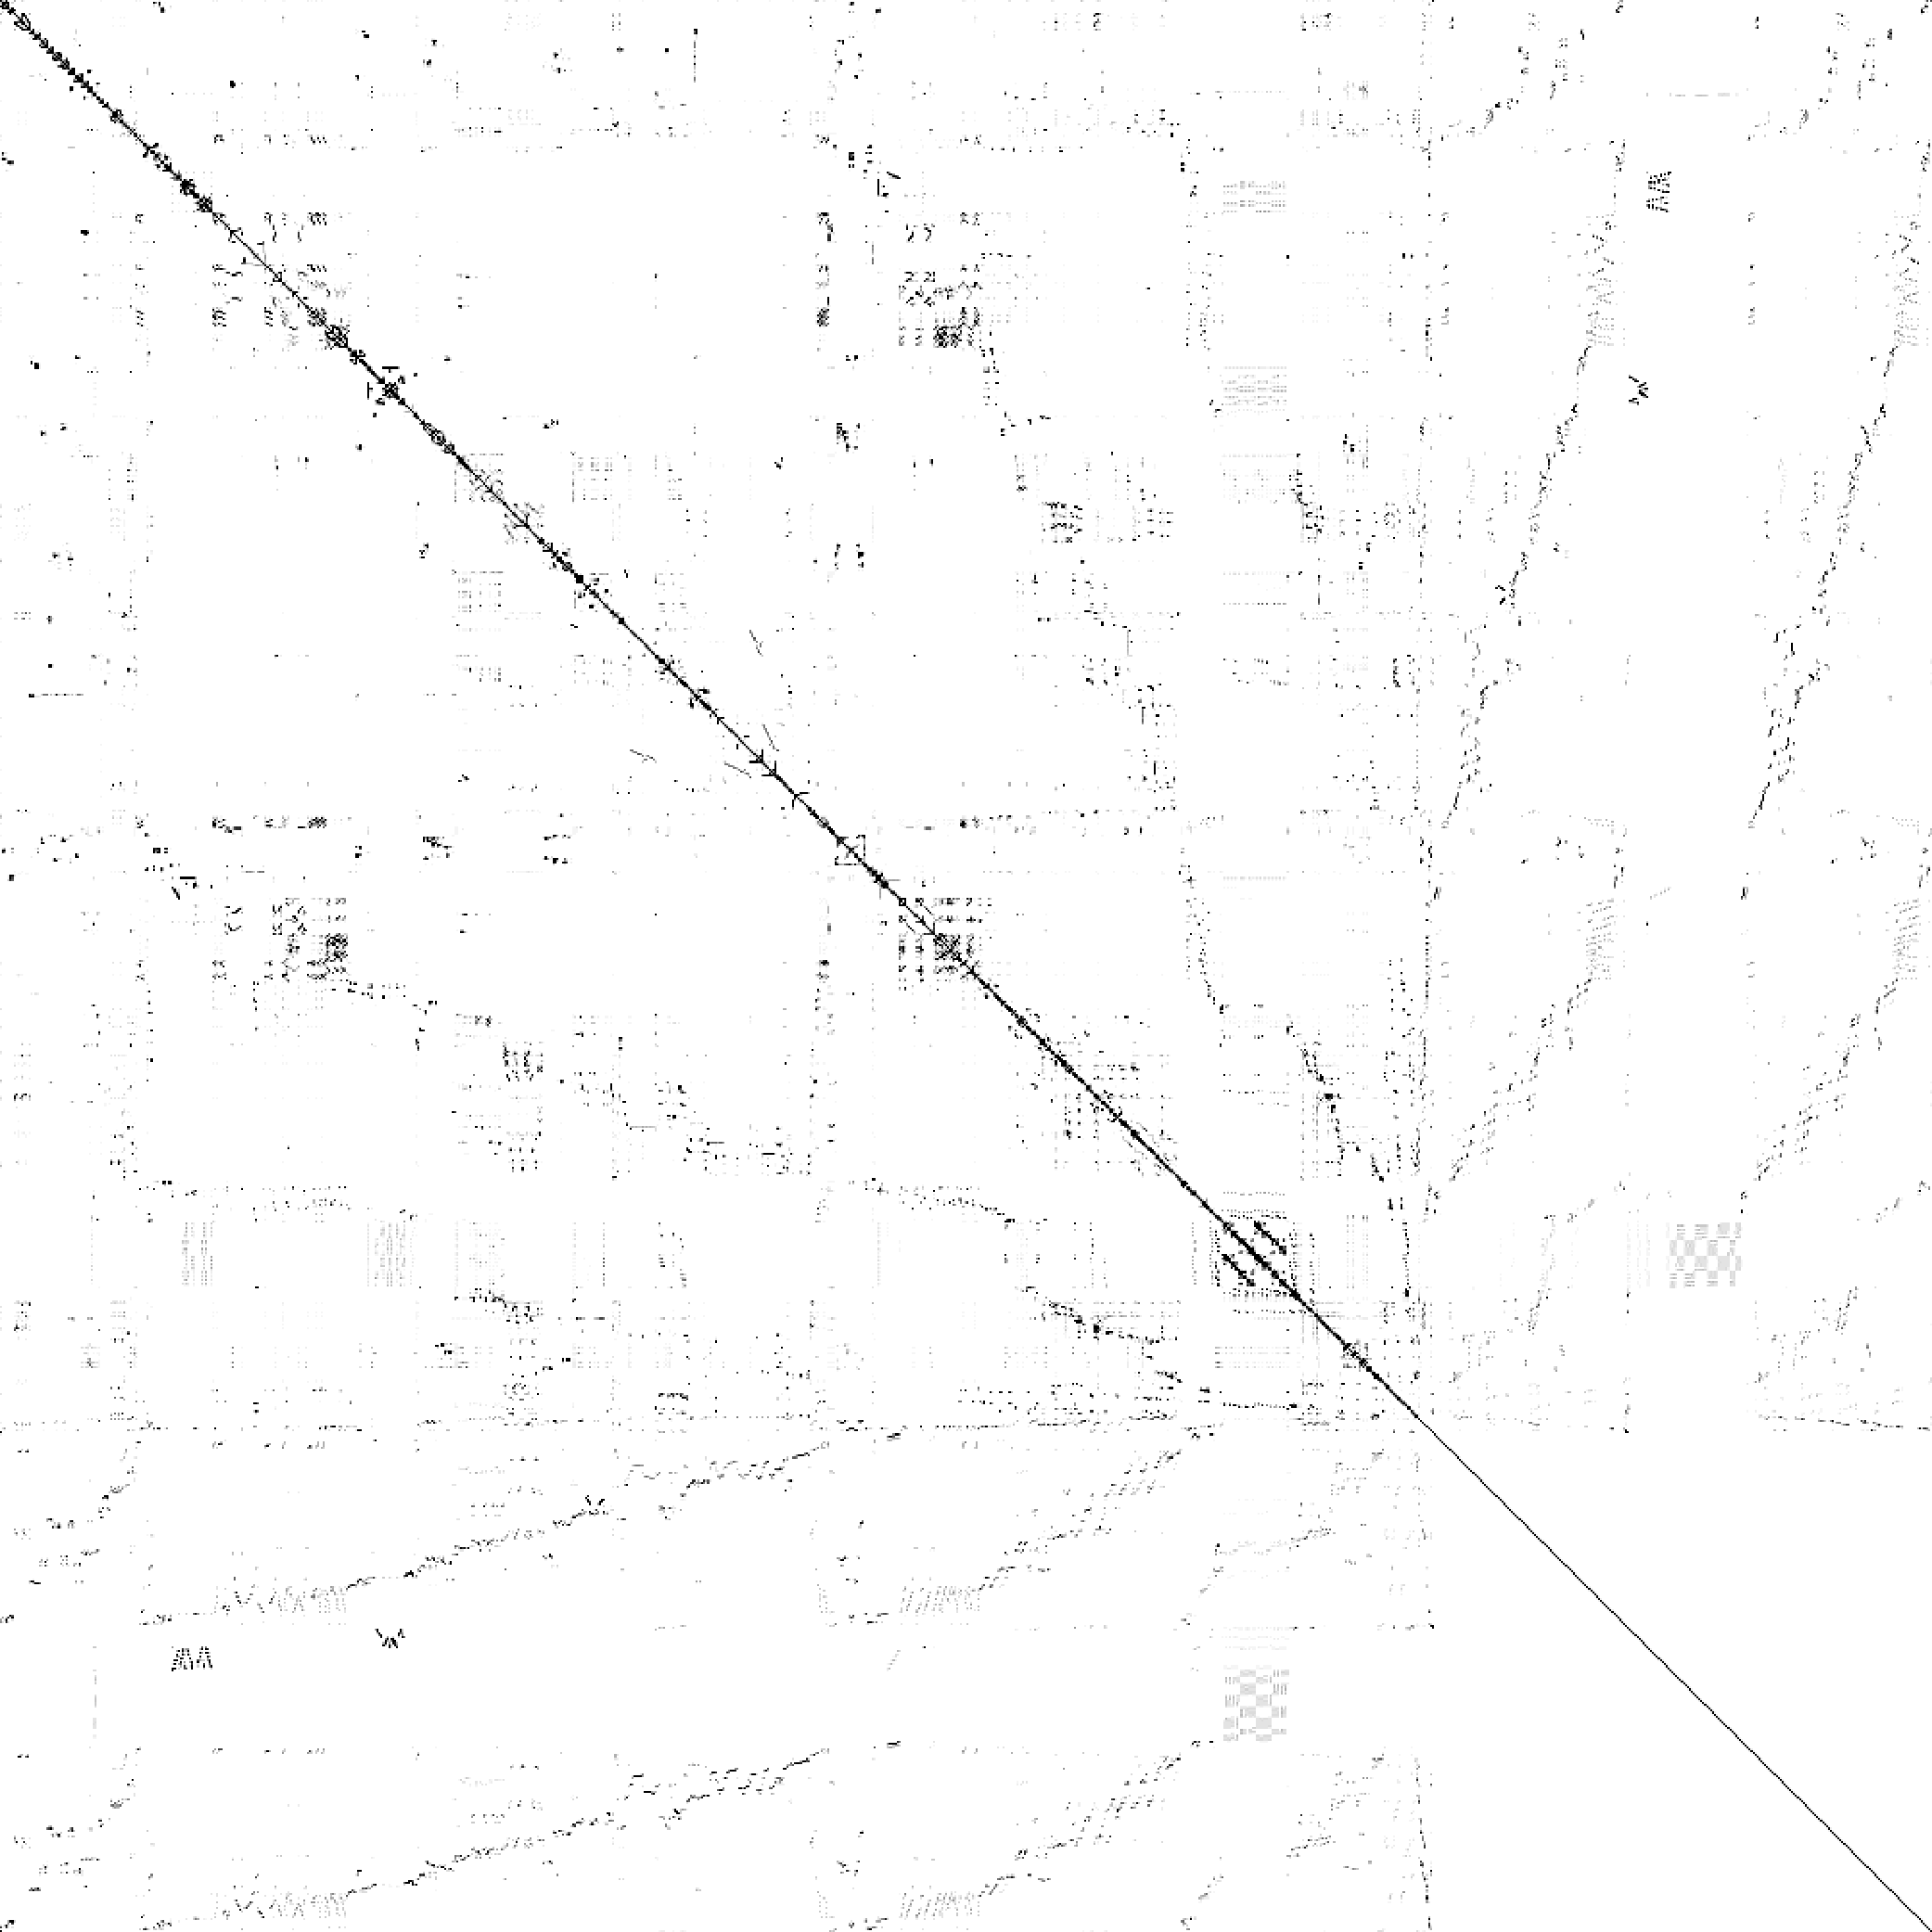
\includegraphics[width=\linewidth]{images/scircuit}
\caption{scircuit}
\end{subfigure}~%
\begin{subfigure}{\linewidth}
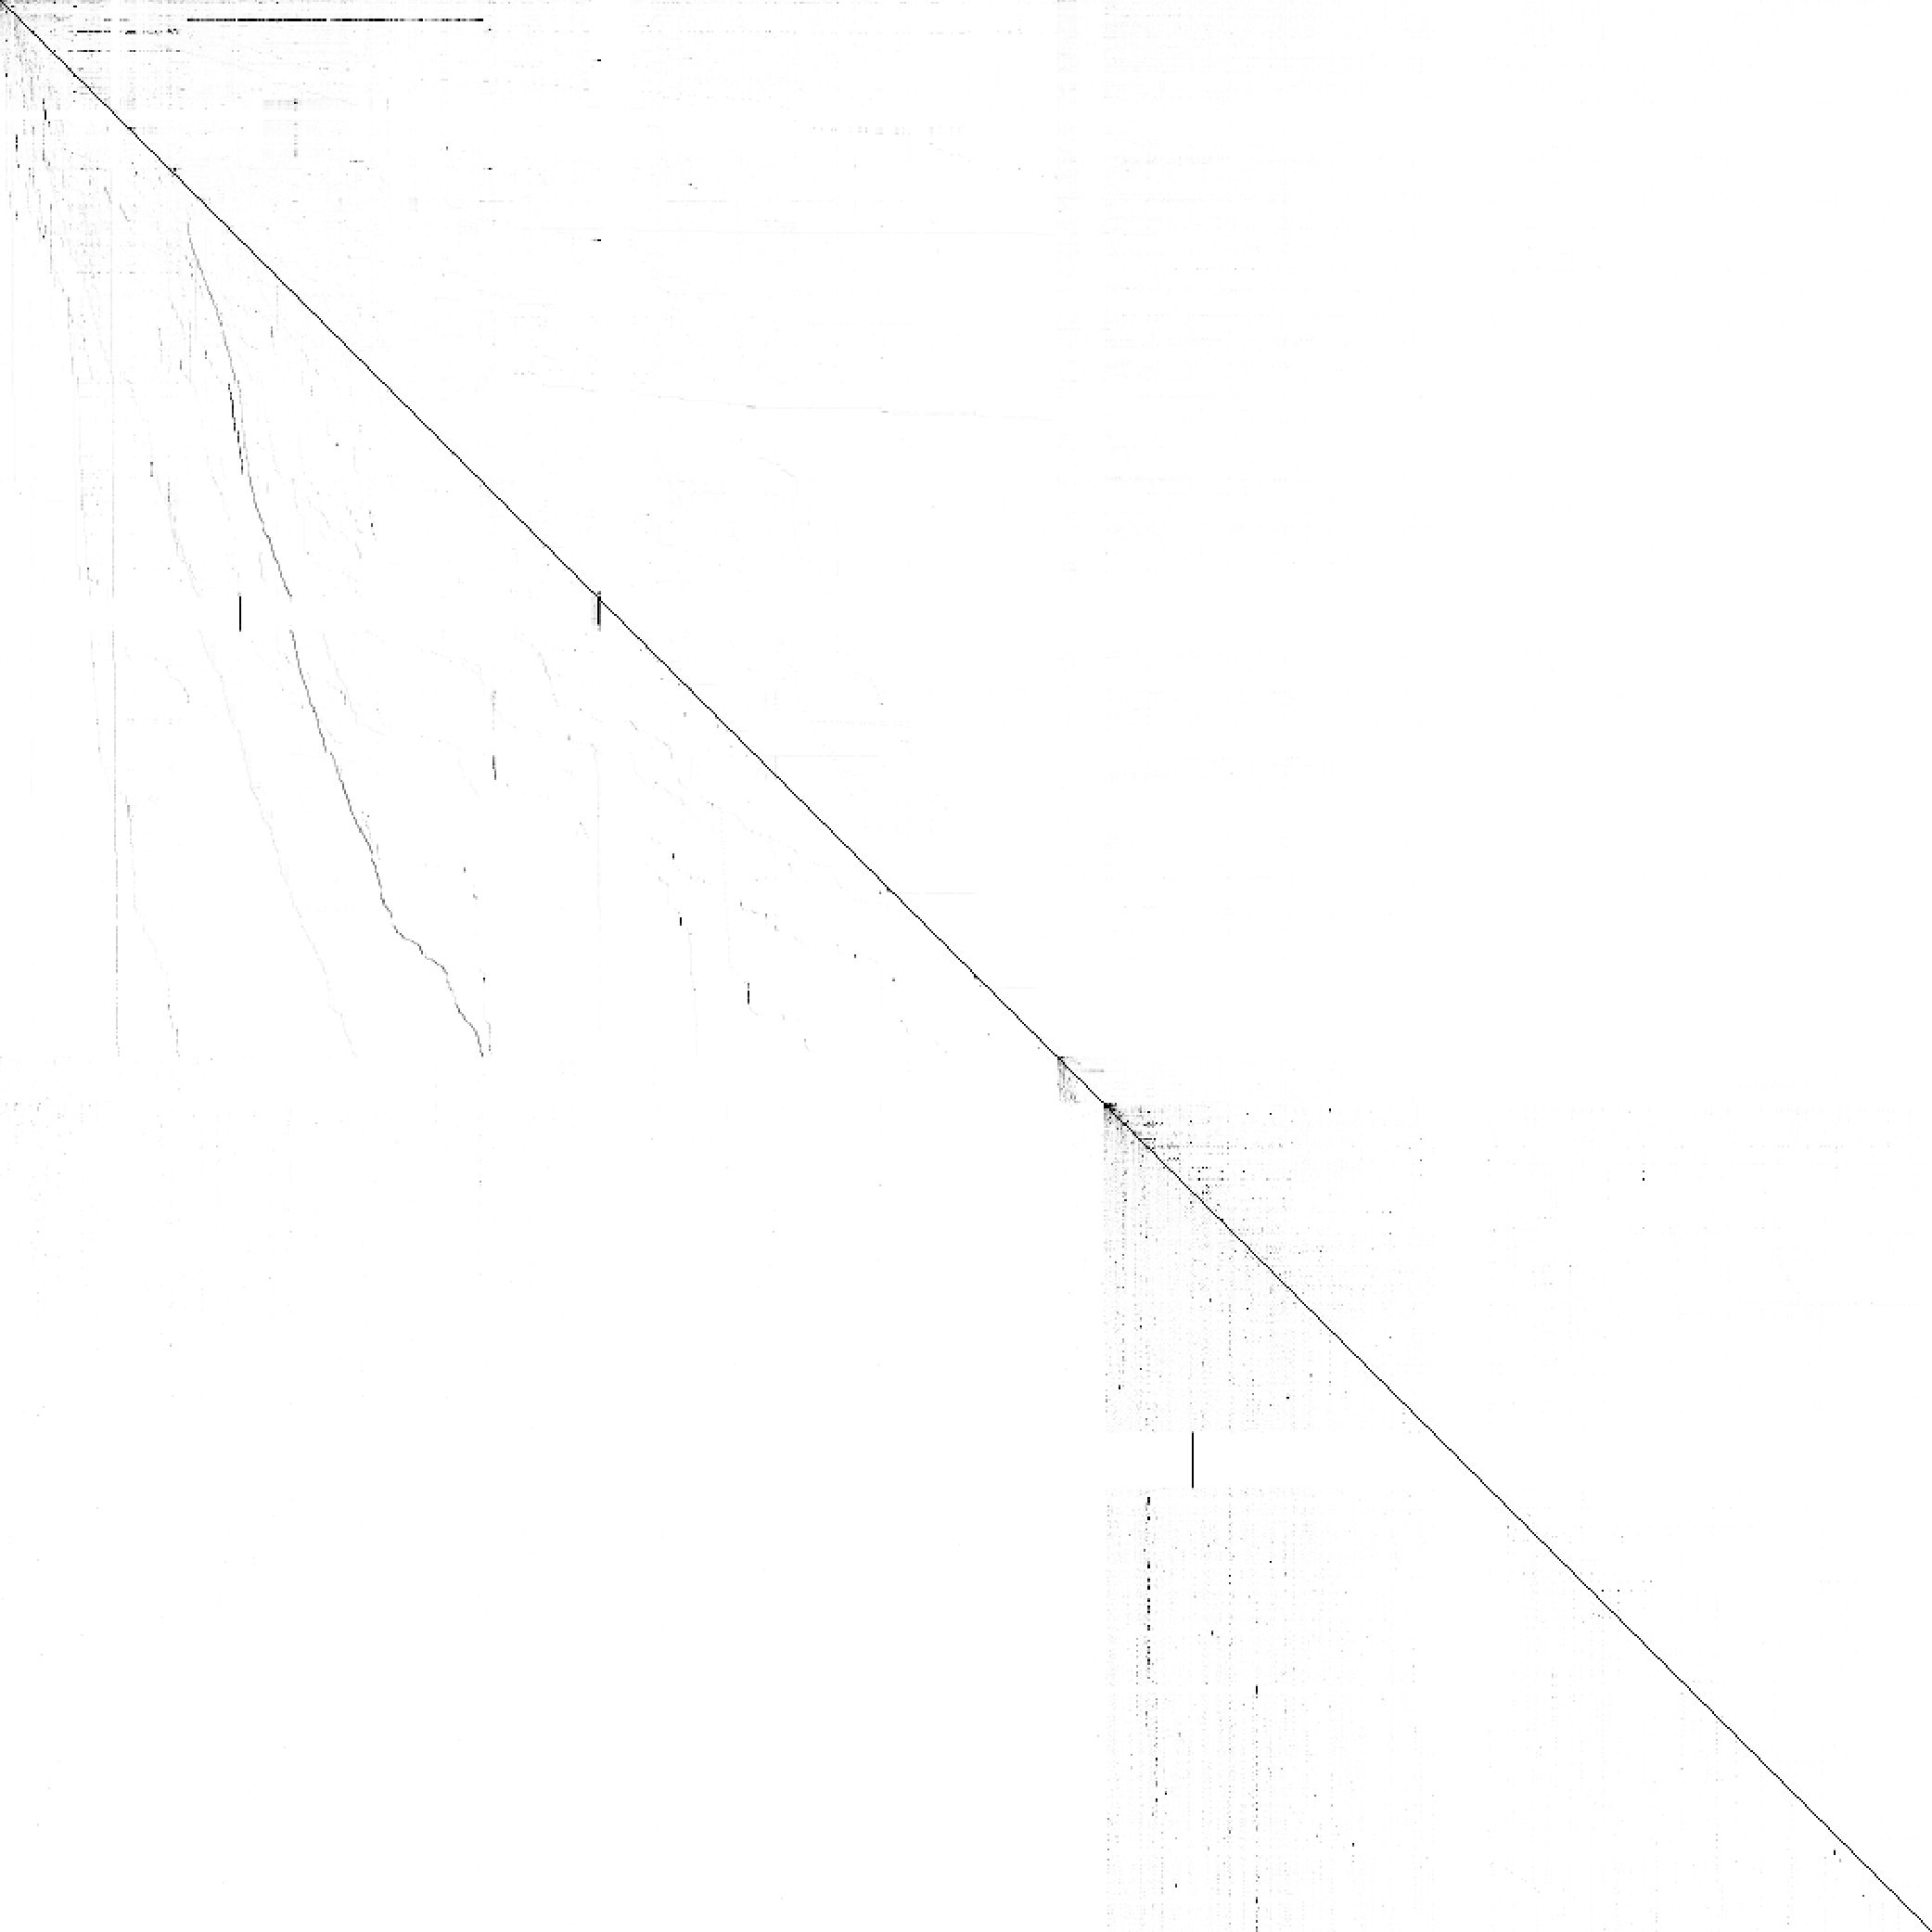
\includegraphics[width=\linewidth]{images/webbase-1M}
\caption{webbase-1M}
\end{subfigure}~%
\end{multicols}
\caption{The density plots of the matrices used for testing}
\end{figure}
\begin{figure}
\centering
\begin{tikzpicture}[scale=.6]
\node at (3,6){FPGA0};
\node at (8.5,6){FPGA1};
\node at (14,6){FPGA2};
\node at (19.5,6){FPGA3};
\foreach \x in {1,...,4,5,6.5,7.5,...,10.5,12,13,...,16,17.5,18.5,...,21.5}
    \foreach \y in {1,...,5}
    {
        %\draw (\x, \y) +(-.5,-.5) rectangle ++(.5,.5);
        %\draw (\x, \y) node{\shortstack{$R^3$\\PE}};
        \draw (\x, \y) node{\shortstack{PE}};
    }
\foreach \x in {1.5,2.5,3.5,4.5,7,8,9,10,12.5,13.5,14.5,15.5,18,19,20,21,22}
{
    \path[draw] (\x, .5) -- (\x, 5.5);
}
\foreach \x in {.5,6,11.5,17}
{
    \foreach \y in {1.5,2.5,3.5,4.5}
    \path[draw] (\x, \y) -- (\x+5, \y);
}
\draw (.5,.5) [rounded corners=.2cm]rectangle (5.5,5.5);
\draw (6,.5) [rounded corners=.2cm]rectangle (11,5.5);
\draw (11.5,.5) [rounded corners=.2cm]rectangle (16.5,5.5);
\draw (17,.5) [rounded corners=.2cm]rectangle (22,5.5);
\foreach \x in {3,8.5,14,19.5}{
    \node at (\x, 3)[draw, fill=white, minimum width=1.8cm, minimum height=1.8cm,inner sep=0,outer sep=0]{\shortstack{Shared\\Memory}};
}
\foreach [count=\i] \x in {0,3.3,6.6,...,24}
{
    \FPeval{\minus}{round(\i-1,0)};
    %\draw (\x, -2) +(-.6,-.5) [rounded corners=.2cm] rectangle ++(1.2, .5);
    \small
    \draw (\x, -2) +(.3, 0) node[rectangle,rounded corners=.2cm]{\shortstack{Memory \\Controller\minus}};
    \normalsize
    %\draw (\x, -2) +(.3, 0) node{\shortstack{MC\i}};
}
\foreach \ae in {3, 8.5, 14, 19.5}
{
    \foreach \mc in {.5,3.8,7.1,...,25}
    {
        \draw[thick] (\ae, .5) -- (\mc, -1.5);
    }
}
%\path[draw, dashed] (.5,-.5) -- (18,-.5);
%\node at (9.25,-.5) [rectangle,fill=white,inner sep=2pt](a){40GB/s Sustained Memory Bandwidth};

\end{tikzpicture}
\caption{$R^3$ implementation on the Convey HC-2 coprocessor: 4 Virtex-5 LX330 FPGAs tiled with 16 $R^3$ SpMV processing elements (PE) each. Each Virtex-5 chip connects to all 8 memory controllers, which enables each chip to have access to all of the coprocessor's memory.}
\label{fig:highlevel}
\end{figure}

\section{Benchmarking}
Ok, now we have a good background about SpMV, the platform it can run on and optimizations for SpMV we need a way to determine who is the best. This when benchmarking comes in. However, different matrices can have vastly different performance. In figure~\ref{nnzVgflops} we show the performance of SpMV on CPUs, GPUs and FPGAs. As you can see the performance is very jumpy from matrix to matrix. 3 factors effect the performance: dimension, sparsity, and values. \par
The dimension of a matrix are the height ($M$), the width ($N$) and the number of nonzeros ($nnz$). These metrics effect different processors differently. \par
For CPUs the $nnz$ and $N$ are important values. As figure~\ref{nnzVgflops} shows when the matrix no longer fits in cache it takes a performance hit. It takes a second performance hit (not shown) when the width of the matrix and the therefor the length of the $x$ vector grows to the point when the $x$ vector also can not fit in cache. \par
For GPUs cache plays less of a role. However, two factors conspire against GPUs. The matrix formats they use and the amount of RAM on GPU boards. The best performing matrix formats of GPUs, ELLPACK and Block-ELLPACK, also introduce 0 values and take up the most memory space. GPU boards currently have at most 12GB of on board RAM compared to the 128 or more possible on CPUs. This means as matrices approach and go beyond 1 billion values then GPUs have to use worse performing matrix formats or be completely unable to perform SpMV. \par
TODO: FPGAs
TODO: sparsity
TODO: values
\begin{figure}
\centering
\begin{tikzpicture}
\draw[step=1.0,gray,very thin] (0,0) grid (6.5,4.5);
\draw [->,thick] (0,0) to (0,5);
\draw [->,thick] (0,0) to (7,0);
\foreach \x/\xtext in {0/1,1/10,2/100,3/1\,000,4/10\,000,5/100\,000,6/1\,000\,000}
	\draw (\x cm, 1pt) -- (\x cm, -1pt) node[anchor=north west,rotate=-30] {$\xtext$};
\foreach \y/\ytext in {0/0,1/4,2/8,3/12,4/16}
	\draw (1pt, \y cm) -- (-1pt,\y cm) node[anchor=east] {$\ytext$};

\foreach \i/\x/\y/\m/\s/\t/\a in {
0/0.0/3.4/dense/1/13.6/.3,%
1/0.0/3.4/rma10/1/13.6/-.1,%
2/0.0/3.2/qcd5\_4/1/12.8/-.4,%
3/2.0293837776852097/3.175/cant/107/12.7/0,%
6/3.5543680009900878/1.55/mc2depi/3584/6.2/.4,%
8/5.0730067708393705/1.475/mac\_econ\_fwd500/118306/5.9/.3,%
9/5.123400785682125/1.975/shipsec1/132862/7.9/.5,%
10/5.433/1.3/raefsky1/271382/5.2/.1,%
11/5.451272036830906/1.55/scircuit/282665/6.2/.3,%
12/5.725640521811938/1.225/psmigr\_2/531668/4.9/-.4,%
13/5.906686753316721/1.6/torso2/806653/6.4/-.1,%
14/6.197264013258786/2.175/consph/1574940/8.7/.3
%1/0/3.4/dense/1/13.6/.3, 1/0/3.4/rma10/1/13.6/-.1, 2/0/3.2/qcd5\_4/1/12.8/-.4, 3/2.03/3.175/cant/107/12.7/0, %
%6/3.5543680009900878/1.55/mc2depi/3584/6.2/.4,%
%8/5.0730067708393705/1.475/mac\_econ\_fwd500/118306/5.9/.3,%
%9/5.123400785682125/1.975/shipsec1/132862/7.9/.5,%
%10/5.451272036830906/1.55/scircuit/282665/6.2/.3,%
%11/5.725640521811938/1.225/psmigr\_2/531668/4.9/-.3,%
%12/5.906686753316721/1.6/torso2/806653/6.4/0,%
%13/6.197264013258786/2.175/consph/1574940/8.7/.3%
}
	\draw (\x,\y) [fill=red]circle (3pt) node[anchor=north west,rotate=60,xshift=4pt, yshift=\a cm, fill=white, inner sep=-2pt]{};

%outliers
\foreach \i/\x/\y/\m/\s/\t/\a in {%
4/2.828015064223977/0.55/dw8192/673/2.2/.6,%
5/3.1408221801093106/1.0/t2d\_q9/1383/4.0/-.1,%
7/4.864689034136851/0.85/epb1/73230/3.4/-.1%
}
	\draw (\x,\y) [fill=yellow]circle (3pt) node[anchor=north west,rotate=60,xshift=.4, yshift=\a cm, fill=white, inner sep=-2pt]{};


\draw [dashed] (2.4,-.6) -- (2.4,4.8) node [midway,above, sloped, xshift=-.5cm]{$256$};
\node at (3,-1.1) {Number of Unique Values in Matrix};
\node at (-.8,2) [rotate=90] {Performance (Gflops)};
\end{tikzpicture}
\caption[dont care]{Unique values in a matrix vs the performance of $R^3$. Matrices with fewer than 256 unique values (only common elements exist) enables $R^3$ format to compress much better. The \tikz \draw[fill=yellow] circle(3pt);'s are outliers due to their size (see Figure \ref{nnzVgflops}).}
\label{uniqueVgflops}
\end{figure}%

\begin{table*}
\caption{Matrix Statistics}
\label{matrix_stat}
\centering
\begin{tabular}{ccccccccc}
\hline
\bfseries Matrix & \bfseries Field & \bfseries dimensions & \bfseries nnz & \bfseries nnz/row \\
\hline
 dense & Example & 2,000x2,000 & 4,000,000 & 2,000 \\
consph & FEM/Speres & 83,334x83,334 & 6,010,480 & 72 \\
cant & FEM/Cantilever & 62,451x62,451 & 4,007,383 & 64 \\
rma10 & FEM/Harbor & 46,835x46,835 & 2,329,092 & 49 \\
qcd5\_4 & QCD & 49,152x49,152 & 1,916,928 & 39 \\
shipsec1 & FEM/ship & 140,874x140,874 & 3,568,176 & 25\\
mac\_econ\_fwd500 & Economics & 206,500x206,500 & 1,273,389 & 6.2 \\
mc2depi & Epidemiology & 525,825x525,825 & 2,100,225 & 4.0 \\
scircuit & Circuit & 170,998x170,998 & 958,936 & 5.6 \\
\hline
%webbase-1M & Webbase & 1,000,005x1,000,005 & 3,105,526 & 3.1 & 565 \\
%\hline
\end{tabular}
\end{table*}
\begin{table*}
\caption{Matrix Statistics}
\label{matrix_stat}
\centering
\begin{tabular}{ccccccccc}
\hline
\bfseries Matrix & \bfseries $\bf R^3$ Gflops & \multirow{1}{*}{\bfseries \shortstack{$\bf 2\times$ Intel E5-2690}} & \multirow{1}{*}{\bfseries \shortstack{Nvidia Tesla M2090}}\\
\hline
 dense &  13.6 & 14 & \bf 23\\
consph &  8.7 & 11 & \bf 15\\
cant &  12.7 & 12 & \bf 17\\
rma10 & 13.6 & \bf 24 & 11\\
qcd5\_4 &  12.8 & \bf 30 & 20\\
shipsec1 & 7.9 & 10 &\bf 11\\
mac\_econ\_fwd500 &  5.9 & \bf 23 & 6\\
mc2depi &  6.2 & 21 & \bf 22\\
scircuit &  6.2 & \bf 12 & 6\\
\hline
%webbase-1M & Webbase & 1,000,005x1,000,005 & 3,105,526 & 3.1 & 565 \\
%\hline
\end{tabular}
\end{table*}
\begin{figure*}
\centering
\begin{tikzpicture}[scale=1]

 \ifthenelse{\equal{\blackandwhite}{true}}{
	\tikzstyle{yellowStar}=[draw, diamond, fill=black!65, inner sep =1.5pt];
	\tikzstyle{blueGreenDiamond}=[draw, diamond, fill=black!75, inner sep =1.5pt];
	\tikzstyle{greenSquare}=[draw, rectangle, fill=black!50, inner sep =2.5pt];
	\tikzstyle{blueTriangle}=[draw, regular polygon, regular polygon sides=3, fill=black!35, inner sep =1.5pt];
 }{
	\tikzstyle{yellowStar}=[draw, star, star points=5, fill=yellow, inner sep =1.5pt];
	\tikzstyle{blueGreenDiamond}=[draw, diamond, fill=green!60!blue, inner sep =1.5pt];
	\tikzstyle{greenSquare}=[draw, rectangle, fill=green, inner sep =2.5pt];
	\tikzstyle{blueTriangle}=[draw, regular polygon, regular polygon sides=3, fill=blue, inner sep =1.5pt];
 }

%\draw [ystep=2.0,gray,very thin, xstep = 14] (0,0) grid (12.9, 6.9);
\draw [->,thick] (0,0) to (14.5, 0);
\draw [->, thick] (0,0) to (0,7);
\foreach \x/\mat/\size in { %
0/dw8192/42K, 1/t2d\_q9/87K, 2/epb1/95K, 3/raefsky1/290K, 4/psmigr\_2/540K, 6/torso2/1M%
}
	\draw (\x cm, 1pt) -- (\x cm, -1pt) node[anchor=east,rotate=90,gray] {\shortstack{\mat (\size)}};
\foreach \x/\mat/\size in { %
5/scircuit/960K, 7/mac\_econ/1.3M, 8/qcd5\_4/1.9M, 9/mc2depi/2.1M, 10/rma10/2.3M, 11/shipsec1/3.6M, 12/dense/4M, 13/cant/4M, 14/consph/6M%
}
	\draw (\x cm, 1pt) -- (\x cm, -1pt) node[anchor=east,rotate=90] {\shortstack{\mat (\size)}};
\foreach \y/\ytext in {0/0,1/5,2/10, 3/15, 4/20, 5/25, 6/30}
	\draw (1pt, \y cm) -- (-1pt, \y cm) node[anchor=east] {$\ytext$};
%\node at (6, -.8) {Size of Matrix (Millions)};
\node at (-1, 3) [rotate=90]{Performance (Gflops)};

%R3 line
\foreach \i/\j/\k/\l in {%
0/0.42000000000000004/1/0.76,  1/0.76/2/0.6599999999999999,  2/0.6599999999999999/3/1.04,  3/1.04/4/0.9800000000000001,  4/0.9800000000000001/5/1.24,  5/1.24/6/1.28,  6/1.28/7/1.1800000000000002,  7/1.1800000000000002/8/2.56,  8/2.56/9/1.24,  9/1.24/10/2.7199999999999998,  10/2.7199999999999998/11/1.58,  11/1.58/12/2.7199999999999998,  12/2.7199999999999998/13/2.54,  13/2.54/14/1.7399999999999998
}{
 \ifthenelse{\equal{\blackandwhite}{true}}{
	\draw [black] (\i,\j) -- (\k,\l);
 }{
	\draw [red] (\i,\j) -- (\k,\l);
 }
}

%hc1 line
\foreach \i/\j/\k/\l in {%
0/0.33999999999999997/1/0.5,  1/0.5/2/0.52,  2/0.52/3/0.78,  3/0.78/4/0.78,  4/0.78/6/0.24
}{
 \ifthenelse{\equal{\blackandwhite}{true}}{
	\draw [black!65] (\i,\j) -- (\k,\l);
 }{
	\draw [brown] (\i,\j) -- (\k,\l);
 }
}

%%tesla line
%\foreach \i/\j/\k/\l in {%
%0/0.1/1/0.18,  1/0.18/2/0.16,  2/0.16/3/0.5599999999999999,  3/0.5599/5/0.6}
%	\draw <3,5>[green!60!blue] (\i,\j) -- (\k,\l);

%m2090 line
\foreach \i/\j/\k/\l in {%
5/1.2/7/1.2,  7/1.2/8/4.0,  8/4.0/9/4.4,  9/4.4/10/2.2,  10/2.2/11/2.2,  11/2.2/12/4.6,  12/4.6/13/3.4,  13/3.4/14/3.0
}{
 \ifthenelse{\equal{\blackandwhite}{true}}{
	\draw [black!50] (\i,\j) -- (\k,\l);
 }{
	\draw [green] (\i,\j) -- (\k,\l);
 }
}

%intel line
\foreach \i/\j/\k/\l in {%
5/2.4/7/4.6,  7/4.6/8/6.0,  8/6.0/9/4.2,  9/4.2/10/4.8,  10/4.8/11/2.0,  11/2.0/12/2.8,  12/2.8/13/2.4,  13/2.4/14/2.2
}{
 \ifthenelse{\equal{\blackandwhite}{true}}{
	\draw [black!35] (\i,\j) -- (\k,\l);
 }{
	\draw [blue] (\i,\j) -- (\k,\l);
 }
}


\draw [dashed] (.5, -.5) -- (.5, 7) node [fill=white,inner sep=0pt, midway,below, sloped]{\small $(64K)$};

\draw [dashed] (10.5, -.5) -- (10.5, 7)  node [fill=white,inner sep=0pt, near end,below, sloped]{\small 20MB $(2.5M)$};



%hc1 points
\foreach \i/\x/\y/\f/\q/\u in {%
0/0.083492/0.33999999999999997/1.7/0/-.2,%
1/0.17405/0.5/2.5/0/-.1,%
2/0.190106/0.52/2.6/0/-.2,%
3/0.588552/0.78/3.9/0/-.2,%
4/1.080044/0.78/3.9/0/-.2,%
6/2.066946/0.24/1.2/0/0
}{
 \ifthenelse{\equal{\blackandwhite}{true}}{
	\draw (\i,\y) node[yellowStar]{} node[fill=white,inner sep=0pt, anchor=west,rotate=30,xshift=\q cm + 3pt, yshift=\u cm] {\color{black!65} \scriptsize $\f$};
 }{
	\draw (\i,\y) node[yellowStar]{} node[fill=white,inner sep=0pt, anchor=west,rotate=30,xshift=\q cm + 3pt, yshift=\u cm] {\color{brown} \scriptsize $\f$};
 }
}	

%intel points
\foreach \i/\x/\y/\f/\q/\u in {%
5/1.917872/2.4/12/0/0,%
7/2.546778/4.6/23/0/0,%
8/3.833856/6.0/30/0/0,%
9/4.20045/4.2/21/0/-.2,%
10/4.658184/4.8/24/0/0,%
11/7.136352/2.0/10/0/0,%
12/8.0/2.8/14/0/.2,%
13/8.014766/2.4/12/0/-.2,%
14/12.02096/2.2/11/0/0
}{
 \ifthenelse{\equal{\blackandwhite}{true}}{
	\draw (\i cm,\y cm) node[blueTriangle]{} node[fill=white,inner sep=0pt, anchor=west,rotate=30,xshift=\q cm + 3pt, yshift=\u cm]{\color{black!50} \scriptsize $\f$};
 }{
	\draw (\i cm,\y cm) node[blueTriangle]{} node[fill=white,inner sep=0pt, anchor=west,rotate=30,xshift=\q cm + 3pt, yshift=\u cm]{\color{blue} \scriptsize $\f$};
 }
}

%M2090 points
\foreach \i/\x/\y/\f/\q/\u in {%
5/1.917872/1.2/6/0/-.3,%
7/2.546778/1.2/6/0/.3,%
8/3.833856/4.0/20/0/0,%
9/4.20045/4.4/22/0/0,%
10/4.658184/2.2/11/0/0,%
11/7.136352/2.2/11/0/.1,%
12/8.0/4.6/23/0/0,%
13/8.014766/3.4/17/0/0,%
14/12.02096/3.0/15/0/0
}{
 \ifthenelse{\equal{\blackandwhite}{true}}{
	\draw (\i,\y) node[greenSquare]{} node[fill=white,inner sep=0pt, anchor=west,rotate=30,xshift=\q cm + 3pt, yshift=\u cm]{\color{black!35} \scriptsize $\f$};
 }{
	\draw (\i,\y) node[greenSquare]{} node[fill=white,inner sep=0pt, anchor=west,rotate=30,xshift=\q cm + 3pt, yshift=\u cm]{\color{green!100} \scriptsize $\f$};
 }
}

%R3 points
\foreach \i/\x/\y/\f/\q/\u in {%
0/0.083492/0.42000000000000004/2.1/0/0,%
1/0.17405/0.76/3.8/0/0,%
2/0.190106/0.6599999999999999/3.3/0/0,%
3/0.588552/1.04/5.2/0/0,%
4/1.080044/0.9800000000000001/4.9/0/0,%
5/1.917872/1.24/6.2/0/0,%
6/2.066946/1.28/6.4/0/0,%
7/2.546778/1.1800000000000002/5.9/0/0,%
8/3.833856/2.56/12.8/0/0,%
9/4.20045/1.24/6.2/0/0,%
10/4.658184/2.7199999999999998/13.6/0/0,%
11/7.136352/1.58/7.9/0/0,%
12/8.0/2.7199999999999998/13.6/0/0,%
13/8.014766/2.54/12.7/0/0,%
14/12.02096/1.7399999999999998/8.7/0/0
}{
 \ifthenelse{\equal{\blackandwhite}{true}}{
	\draw (\i,\y) [fill=black]circle(3pt) node(r\i)[fill=white,inner sep=0pt, anchor=west,rotate=30,xshift=\q cm + 3pt, yshift=\u cm]{\color{black} \scriptsize $\f$}; 
 }{
	\draw (\i,\y) [fill=red]circle(3pt) node(r\i)[fill=white,inner sep=0pt, anchor=west,rotate=30,xshift=\q cm + 3pt, yshift=\u cm]{\color{red} \scriptsize $\f$};
 }
}

\draw (4,5.5) node (key)[rectangle,minimum width=4cm, minimum height=2.7cm]{};
 \ifthenelse{\equal{\blackandwhite}{true}}{
	\node at (key) [rectangle,anchor=west, xshift=-2cm, yshift=1cm]{\tikz{\draw (0,1pt) [fill=black]circle (2.5pt);} $R^3$};
 }{
	\node at (key) [rectangle,anchor=west, xshift=-2cm, yshift=1cm]{\tikz{\draw (0,1pt) [fill=red]circle (2.5pt);} $R^3$};
 }
\node at (key) [rectangle,anchor=west, xshift=-2cm, yshift=.3cm]{\shortstack{\tikz{\draw (0,1pt) node[yellowStar]{};} \cite{prelim:nagar1} }};
%\node <3,5>at (key) [rectangle,anchor=west, xshift=-2cm, yshift=0cm]{\tikz{\draw (0,1pt) node[blueGreenDiamond]{};} Nvidia Tesla S1070};
\node at (key) [rectangle,anchor=west, xshift=-2cm, yshift=-.5cm]{\shortstack{\tikz{\draw (0,1pt) node[greenSquare]{};} Nvidia Tesla \\M2090}};
\node at (key) [rectangle,anchor=west, xshift=-2cm, yshift=-1.5cm]{\shortstack{\tikz{\draw (0,1pt) node[blueTriangle]{};} Intel E5-2690 \\(2 CPUs)}};

\end{tikzpicture}
\caption{$nnz$ vs Performance on each platform. The small matrices, ones around 64K or less, performed poorly on $R^3$, due to the overhead. CPUs experience the opposite effect. They take a performance hit once the matrix no longer fits in cache.}
\label{nnzVgflops}
\end{figure*}

\chapter{SpMV on FPGA METHODOLOGY}
\label{chp:method}

\begin{figure}
    \centering
    \begin{tikzpicture}[scale=2]
        \draw (0,0) rectangle (4,.1);
        \draw (.1,.1) rectangle (3.9,.2);
        \draw (.2,.2) rectangle (3.8,.3);

        \draw (.3,.3) rectangle (1.1,.5);
        \draw (1.6,.3) rectangle (2.4, .5);
        \draw (2.9, .3) rectangle (3.7, .5);
        \draw (.4,.5) rectangle (1,2.5);
        \node at (.7,1.5) [rotate=90]{\shortstack{Matrix\\Traversal}};

        \draw (1.7,.5) rectangle (2.3,2.5);
        \node at (2,1.5) [rotate=90]{\shortstack{Multiply-\\accumulator}};

        \draw (3,.5) rectangle (3.6,2.5);
        \node at (3.3,1.5) [rotate=90]{\shortstack{Matrix\\Compression}};

        \draw (.3,2.5) rectangle (1.1,2.7);
        \draw (1.6,2.5) rectangle (2.4, 2.7);
        \draw (2.9, 2.5) rectangle (3.7, 2.7);

        \draw (.2,2.7) -- (3.8,2.7) -- (3.8,3) -- (2,3.7) -- (.2,3) -- cycle;
        \draw (.3,2.8) -- (3.7,2.8) -- (3.7, 2.92) -- (2,3.59) -- (.3,2.92) -- cycle;
        \node at (2,3.1) {\shortstack{Computing\\SpMV on FPGAs}};
    \end{tikzpicture}
    \caption{Because different aspects limit the performance of SpMV on FPGAs, no one optimization will lead to significant benefit for SpMV. We identified these three optimizations that together lead to a significant performance benefit.}
    \label{fig:pillars}
\end{figure}

In the previous chapter, we have discussed how others have approached computing SpMV on FPGAs and other processors. We build upon some of the good ideas and add our own. When these pillars are in place the dataflow of the design still looks the same as other implementations (\figurename~\ref{fig:dataflow}). The architecture diagram also follows the same general flow of the dataflow diagram (\figurename~\ref{fig:SpMV}).
Three pillars emerged during the design of the hardware description and software: designing the traversal of the matrix, designing the multiply-accumulator, and designing the matrix compression (\figurename~\ref{fig:pillars}). The next three sections describe these pillars and the interactions between them.

\section{First Pillar: Matrix Traversal}
\par The first pillar, matrix traversal, primarily helps with vector reuse. Column traversal has a major effect on vector reuse. Many papers argue that vector caching is the way to achieve $x$ vector reuse for FPGAs [\cite{prelim:umuroglu, prelim:nagar1}] (TODO: more cites). We disagree. With the ability to use column traversal in a horizontal subsection of say 1000 rows one can perfectly reuse vector values in this section. This requires the storage of 1000 intermediate y values or 8KB. Compare this to caching. Assume there are 10 non-zero elements per row and assume each vector value gets accessed twice. Then to achieve good caching the cache must support 5000 values or 40KB. This also ignores storing the vector indices of the cached values. So, in this example, storing intermediate values is more than 5 times more space efficient than vector caching.
\par The second advantage of mixing row and column traversal is that it leads to smaller deltas. In this paper, a delta is the traversal distance between a matrix element and its preceding matrix element in the traversal. To achieve high $x$ vector reuse and small deltas we use row-column-row traversal. Chapter \ref{chp:traversal} discusses matrix traversal in detail.

\section{Second Pillar: Multiply-accumulator}

\par The second pillar, the multiply accumulator, has to accumulate multiple rows at a time to allow different traversals (the first pillar). Several multiply-accumulators exists, but they rely on row-major traversal \cite{}. Although, we do use pre-existing floating-point cores created by Flopoco [\cite{}]. We created an IP core called the Intermediator, which stores intermediate $y$ values and allows for row-column-row traversal. Chapter \ref{chp:mac} discusses the multiply-accumulator in detail.

\section{Third Pillar: Matrix Compression}
\par The third pillar, compression, may be the most important for FPGAs. Compression of the matrix has a large amount of importance, because reading the matrix takes up a majority of the memory bandwidth. The current view in the SpMV field does not count preprocessing of the matrix towards the SpMV runtime. This is because SpMV is usually used in iterative and repetitive methods. We agree with this sentiment.
\subsection{Index compression}
\par Using deltas to compress indices is the first and easiest step towards this pillar. Many compression implementations try to align variable length encoding to 4 bit or other size boundaries. We give little regard to boundaries because we find the added compression to be worth the extra FPGA space the decoder needs. Chapter \ref{chp:compression} discusses delta compression in detail.
%
\subsection{Floating Point Compression}
\par Value compression is tricky but has a potential to save large amounts of space and thus memory bandwidth. Values repeat more than one would expect in matrices \cite{}. Taking advantage of this repetition is the biggest step towards good compression. \figurename~\ref{fig:uniqueVgflops} shows how much of an effect this pattern has on the performance of our previous SpMV implementation, $R^3$. Chapter \ref{chp:fzip} discusses floating point compression in detail.

\subsection{Multi-port Shared Memory}
\par Because good value compression requires a significant amount of on-chip memory space, we designed a shared memory IP block. This means instead of using 1 RAM block on each PE to store the 512 most common floating point values, we use one RAM block per PE to create a large shared memory to store the 8,192 most common floating point values. Chapter \ref{chp:memory} discusses the design of the shared memory IP block.%
%
\begin{figure}
\centering
\begin{tikzpicture}[scale=1]
\draw [dashed](-6,0) -- (4,0);
\node at (.1,-2) {\large \shortstack{External\\Memory}};
\node at (.1,-1) [draw, trapezium, trapezium right angle=70, trapezium left angle=-70,  minimum width=1.5cm, minimum height=1cm, inner xsep=-7pt](x){$x$ Vector};
\node at (-3,-1.25) [draw,trapezium, trapezium right angle=70, trapezium left angle=-70,  minimum width=1.5cm, minimum height=1.5cm, inner xsep=-12pt](a){$A$ Matrix};
\node at (2.5,-1) [draw, trapezium, trapezium right angle=70, trapezium left angle=-70, minimum width=0cm, minimum height=1cm, inner xsep=-7pt](y){$y$ Vector};

\node at (0, 3) {\large $R^3$ Processing Element};
\draw [dashed] (-6,1.5) -- (-3,1.5);
\node at (-4.5, 1.5) [draw, rectangle, minimum height=2cm, minimum width=3cm](dec){};
\node at (-5.3,1.5)[rotate=90, anchor=south,fill=white]{Decoder};
\node at (-4.5,2) {Value};
\node at (-4.5,1) {Index};
\node at (-4.5, 3.5) [color=black](vCache){Shared Memory};
\path [draw, color=black] (vCache.north east) to (vCache.south east) to (vCache.south west) to (vCache.north west);
\node at (1,1.5) [draw, rectangle, minimum height=2.1cm, minimum width=5cm, label={[label distance=-.5cm]90:Multiply-Accumulator}](acc){};
\node at (acc) [draw, rectangle, xshift=1.8cm, yshift=-.2cm, minimum height=1cm](add){Adder};
\node at (acc) [draw, rectangle, xshift=0cm, yshift=-.2cm, minimum height=1cm](int){\shortstack{Inter-\\mediator}};
\node at (acc) [draw, rectangle, xshift=-1.8cm, yshift=-.2cm, minimum height=1cm](mult){\shortstack{Multi-\\plier}};

\path [draw, thick, >=stealth',->, shorten >=2pt](a) to [] node[fill=white, inner sep=1pt, pos=.4]{\shortstack{val+\\row+col}}(dec);
\path [draw, thick, >=stealth',->, shorten >=2pt, label={[above,sloped]{column}}](dec) to [] node[sloped, fill=white, inner sep=1pt]{col} (x);
\path [draw, thick, >=stealth',->, shorten >=2pt](dec.20) to node[sloped, fill=white, inner sep=1pt]{val} (mult);
\path [draw, thick, >=stealth',->, shorten >=2pt](dec.-20) to node[sloped, fill=white, inner sep=1pt]{row} (mult);
\path [draw, thick, >=stealth',->, shorten >=2pt](mult.120) to [bend left = 30] node[sloped, fill=white, inner sep=1pt]{val+row} (int);

\path [draw, thick, >=stealth',->, shorten >=2pt](x) to [] node[sloped, fill=white, inner sep=1pt]{val} (mult);
\path [draw, thick, >=stealth',->, shorten >=2pt](int.north) to [bend left = 20] node[sloped, fill=white, inner sep=1pt]{val+val+row} (add.50);
\path [draw, thick, >=stealth',->, shorten >=2pt](add.-50) to [bend left = 40] node[sloped, fill=white, inner sep=1pt]{val+row} (int);
\path [draw, thick, >=stealth', ->, shorten >= 2pt](int) .. controls (1,0) and (2.1,0) .. node[sloped, fill=white, inner sep=1pt]{val}  (y);
\path [draw, gray, thick, >=stealth', <->, shorten >=2pt] (vCache) -- (dec);

\end{tikzpicture}
\caption[Diagram of a single processing element]{A single processing element. The arrows show the flow of data through the processing element. Although this diagram shows the memory access to each of the 3 places in memory as separate, they share one memory port. The diagram also does not show the FIFOs that help keep the pipeline full.}
\label{fig:SpMV}
\end{figure}%
%

\begin{figure}
\centering
\begin{tikzpicture}[scale=.6]
\node at (3,6){FPGA0};
\node at (8.5,6){FPGA1};
\node at (14,6){FPGA2};
\node at (19.5,6){FPGA3};
\foreach \x in {1,...,4,5,6.5,7.5,...,10.5,12,13,...,16,17.5,18.5,...,21.5}
    \foreach \y in {1,...,5}
    {
        %\draw (\x, \y) +(-.5,-.5) rectangle ++(.5,.5);
        %\draw (\x, \y) node{\shortstack{$R^3$\\PE}};
        \draw (\x, \y) node{\shortstack{PE}};
    }
\foreach \x in {1.5,2.5,3.5,4.5,7,8,9,10,12.5,13.5,14.5,15.5,18,19,20,21,22}
{
    \path[draw] (\x, .5) -- (\x, 5.5);
}
\foreach \x in {.5,6,11.5,17}
{
    \foreach \y in {1.5,2.5,3.5,4.5}
    \path[draw] (\x, \y) -- (\x+5, \y);
}
\draw (.5,.5) [rounded corners=.2cm]rectangle (5.5,5.5);
\draw (6,.5) [rounded corners=.2cm]rectangle (11,5.5);
\draw (11.5,.5) [rounded corners=.2cm]rectangle (16.5,5.5);
\draw (17,.5) [rounded corners=.2cm]rectangle (22,5.5);
\foreach \x in {3,8.5,14,19.5}{
    \node at (\x, 3)[draw, fill=white, minimum width=1.8cm, minimum height=1.8cm,inner sep=0,outer sep=0]{\shortstack{Shared\\Memory}};
}
\foreach [count=\i] \x in {.5,3.8,7.1,...,25} %0,3.3,6.6,...,24}
{
    \FPeval{\minus}{round(\i-1,0)};
    %\draw (\x, -2) +(-.6,-.5) [rounded corners=.2cm] rectangle ++(1.2, .5);
    \small
    \draw (\x, -1.5) node[draw, rectangle,rounded corners=.2cm,rotate=90,anchor=east]{\shortstack{Memory \\Controller~\minus}};
    \normalsize
    %\draw (\x, -2) +(.3, 0) node{\shortstack{MC\i}};
}
\foreach \ae in {3, 8.5, 14, 19.5}
{
    \foreach \mc in {.5,3.8,7.1,...,25}
    {
        \draw[thick] (\ae, .5) -- (\mc, -1.5);
    }
}
%\path[draw, dashed] (.5,-.5) -- (18,-.5);
%\node at (9.25,-.5) [rectangle,fill=white,inner sep=2pt](a){40GB/s Sustained Memory Bandwidth};

\end{tikzpicture}
\caption[Modified high-level diagram of the Convey HC-2ex]{Our implementation has one shared memory for storing repeating values in the sparse matrices.}
\label{fig:highlevel2}
\end{figure}
\section{High Level Design}
Designing high performance reconfigurable computing implementations has a general two step process, which we follow. First, design one processing element (PE) to solve the problem (see \figurename~\ref{fig:SpMV}). Second, replicate that PE until all the FPGAs are full. In addition, we have a shared memory (see \figurename~\ref{fig:highlevel2}).

The PEs recieve instructions through a 1D systolic array. Each PE has 14 registers. Each PE has 8 instructions: RESET, READ\_REGISTER, WRITE\_REGISTER, WRITE\_DELTA\_CODES, WRITE\_FZIP\_CODES, WRITE\_SHARED\_MEMORY, and COMPUTE\_SPMV.

The PE themselves have 2 major components. First, the decoder block that requests the compressed matrix data and decodes it into row and column indices and floating point values. Second, the multiply-accumulator, where the actual SpMV computation takes place.

To Parallelize the SpMV computation we split the problem into $N$ smaller SpMV computations each given to one processing element. In hardware we connect each processing element to an external memory port and a shared memory port. Chapter \ref{chp:memory} discusses the high level design in detail.
%\par We separate our contributions into 5 pieces, the next 5 chapters. Chapter~\ref{chp:mac} focuses entirely on the first pillar, the multiply accumulator design. Chapter~\ref{chp:compression} focuses on pillars 2 and 3 with discussing matrix traversal and compressing indices with delta compression. Chapter~\ref{chp:fzip} focuses on the second part of pillar 3, value compression. We found good value compression requires a large amount of on-chip memory, therefore, Chapter~\ref{chp:memory} focuses on the design of a large memory shared by multiple processing elements.

\include{Body/chapter_matrix_traversal}
\chapter{MULTIPLY-ACCUMULATOR}
\label{chapter:mac}
\begin{figure}
\hspace{-10pt}
\begin{tikzpicture}[scale=1]
\clip (-5,-2.5) rectangle (5,2.5);
\node at (0,0) [draw, rectangle, minimum height=4cm, minimum width=8cm, label={[label distance=-.6cm,xshift=-2cm]90:Multiply-Accumulator}](acc){};
\node at (acc) [draw, rectangle, xshift=3cm, yshift=0cm, minimum height=1cm, minimum width=2cm](add){Adder};
\node at (acc) [draw, rectangle, xshift=.3cm, yshift=0cm, minimum height=1cm, minimum width=0](int){\shortstack{Intermediator}};
\node at (acc) [draw, rectangle, xshift=-3cm, yshift=0cm, minimum height=1cm, minimum width=2cm](mult){\shortstack{Multiplier}};

\path [draw, thick, >=stealth',->] (-5,.3) --node[ fill=white, inner sep=1pt]{val} (-4,.3) ;
\path [draw, thick, >=stealth',->] (-5,0) --node[ fill=white, inner sep=1pt]{val} (-4,0) ;
\path [draw, thick, >=stealth',->] (-5,-.3) --node[ fill=white, inner sep=1pt]{row} (-4,-.3);

\path [draw, thick, >=stealth',->] (-2,0) --node[ fill=white, inner sep=1pt]{val} (-1,0);
\path [draw, thick, >=stealth',->] (-2,-.3) --node[ fill=white, inner sep=1pt]{row} (-1,-.3) ;

\path [draw, thick, >=stealth',->] (.4,.5)  arc(160:20:1.2);
\node at (1.5,1.2)[fill=white, inner sep=1pt]{row};

\path [draw, thick, >=stealth',->] (.1,.5)  arc(163:17:1.5);
\node at (1.5,1.5)[fill=white, inner sep=1pt]{val};

\path [draw, thick, >=stealth',->] (-.2,.5)  arc(166:14:1.8);
\node at (1.5,1.8)[fill=white, inner sep=1pt]{val};

\path [draw, thick, >=stealth',->] (2.6,-.5)  arc(-20:-160:1.2);
\node at (1.5,-1.2)[fill=white, inner sep=1pt]{row};

\path [draw, thick, >=stealth',->] (2.9,-.5)  arc(-17:-163:1.5);
\node at (1.5,-1.5)[fill=white, inner sep=1pt]{val};

\path [draw, thick, >=stealth',->] (-.5,-.5) --node[sloped, fill=white, inner sep=1pt]{val} (-.5,-2.5);
\end{tikzpicture} %

\caption{The no-stall multiply-accumulator block handles multiple intermediate values at a time. This allows multiple intermediate values in the adder pipeline.}
\label{mac}
\end{figure}
A high throughput SpMV implementation relies on designing a no-stall multiply accumulator (MAC). An inefficient engine stalls when a matrix and its associated vector value arrives every or nearly every clock cycle. The long latency of floating point addition makes this hard. To solve this, our approach works on multiple intermediate $y$ vector values and does the additions out of order. For example in computing $1+2+3+4$ the MAC does $(1+2)+(3+4)$. This removes the data dependency of adding $1$ and $2$ before processing $3$. CPUs and GPUs compute floating point addition in order (eg. $((1+2)+3)+4$). This means results may differ slightly, because changing the order of floating point addition can change the result [\cite{prelim:goldberg}].\\
\indent In $R^3$ [\cite{prelim:townsend}] we designed a block called an Intermediator (Section \ref{sec:intermediator}) capable of storing 32 intermediate $y$ vector values. In our next design we intend to expand this to 1024 (the depth of one dual port BlockRAM in most Xilinx chips). Both designs have an interesting side effect that the allow the matrix to be traversed in a loosely row major traversal and the MAC will still work correctly. The step to from 32 to 1024 intermediate values allows more freedom in the traversal. The rest of the chapter discusses the new design. The matrix elements in one set of 512 rows can be traversed in any way just as long as all the elements are traversed before going to the next 512 rows. Later in chapter 5 we discuss traversals that abide by this rule and allow for easy reuse of $x$ vector values. We plan to use a traversal that follows this rule called row column row (RCR) traversal.
\section{Intermediator}
\label{sec:intermediator}
The Intermediator (Figure \ref{intermediatorEx}) takes in two values, one from the multiplier's result and one from the adder's result and outputs a pair of values to be added. The dual-port Block RAM (middle block in Figure \ref{intermediatorEx}) stores intermediate values until an element in the same row appears. \par
For most matrices, the Block RAM cannot store the entire intermediate $y$ vector. Also the control logic needs to remember the state of each slot in RAM (empty or full). Remembering the state of each RAM location and updating that state requires complicated logic. In $R^3$ we approach this problem by limiting the number of active intermediate values to 32. In our new design we will use a distributed RAM with width of 1 bit to keep track of the state of each slot. Since distributed RAM only has 1 write port we need to do something clever. The first option would be to multi-pump the distributed RAM to achieve two writes every clock cycle. The second option is to create a dual port RAM with Banking. Banking is discussed in chapter 9. The third option is to use 4 RAM blocks and clever use of XORs.
\par The memory has four states with we call the red, yellow, green and white states. The memory is partitioned into 2 parts an upper and lower part. Once the accumulation starts one of these parts will be in the red active state. Once the incoming values move to the next 512 row section of the matrix the active state transitions to the yellow fading state, and the other half of the memory is now in the active state. Recall our traversal rule is that each 512 rows must be traversed before proceeding to the next 512 rows. The yellow fading state exists because values are still being accumulated in the previously active memory. The memory will always be accumulated in 80 clock cycles. At that point the faded state transitions to the green ``read to store" state. Once the values have been sent out to be stored the memory transitions to the white idle state.
\par To understand why 80 cycle cycles are needed to ensure the accumulation has finished after no new values arrive from the multiplier, let us look at the worst case. Only inputs from the adder correspond with to the elements in the fading window. So, the theoretical worst case occurs with a full adder pipeline and each value corresponds to the same row. Every 16 cycles (the adder pipeline length) the number of elements with the same row in the pipeline cuts in half. Therefore the worst case would take 80 ($(log_2(16) + 1) \times 16$) clock cycles to guarantee that the fading window only has final $y$ vector values. The worst case would also advance the window in 512 clock cycles (1 element per row in the matrix for those 512 rows corresponding to the active window). It also takes 512 cycles to store the green "ready to store" elements. So in theory the MAC could stall, but in practice this never happens.
\par Many cases occur when accumulating values in multiple rows and the Intermediator handles each case properly:
\\\indent Case 1: (Figure \ref{cycle7}) The trivial case, no valid input arrives. If the ``to result" block has values, it outputs a value. An overflow FIFO (explained in case 6) outputs a value if it has values.
\\\indent Case 2: (Figure \ref{cycle4}) Only one value arrives (valid) and the row corresponds to an empty cell. The value goes into the empty cell. If the ``to result" window has values, it outputs a result, and if the FIFO has values it outputs a set to the adder.
\\\indent Case 3: (Figure \ref{cycle1}) Similar to case 2 except with a full cell. It retrieves the value in the ram slot and goes to the adder with the input value. The state of the cell gets updated to empty.
\\\indent Case 4: (Figure \ref{cycle2}, \ref{cycle8}) Both values have row indexes that correspond to empty cells in the Block RAM. Both values get stored in the Block RAM and both cells switch to full. If the FIFO from the Block RAM to the output has values it sends one set of values to the output. 
\\\indent Case 5: (Figure \ref{cycle6}) One value has a row index corresponding to an empty cell, and the other to a full cell. The first value goes in the empty cell and the full cell goes to the output with the second value. 
\\\indent Case 6: (Figure \ref{cycle3}) Both values have row indexes that correspond to full cells in the Block RAM. One input value and corresponding Block RAM cell goes to the output. The output can only handle one output pair at a time, so the other input value and corresponding Block RAM cell goes to the FIFO.
\\\indent Case 7: (Figure \ref{cycle5}) The inputs Row0 and Row1 equal each other. In this case the the values go through the pipeline and do not use the Block RAM in the center of the block. They simply pass through to the adder with the row index.\\
%
\begin{figure*}
\begin{multicols}{3}
\begin{subfigure}{\linewidth}
\begin{tikzpicture}
\node (a) {Input};
\node (b)[below=of a] {Result};
\node (c)[right=of a,xshift=-.6cm,yshift=.2cm] {RAM};
\draw (c) +(-.5,0.2) rectangle ++(.5,-2.2);
\node (d)[xshift=-.7cm,yshift=-.5cm,right=of c, draw, minimum width=1.5cm, minimum height=.5cm, label=above:FIFO]{};
\node (e1) at ([xshift=-.6cm]d) [draw, rectangle, minimum height=.5cm, minimum width=.3cm,pattern=north east lines]{};
\node (e)[below=of d, yshift=.3cm]{Adder};
%\node (f) at ([yshift=-2cm]c) [draw,minimum width=1.5cm]{};
%\coordinate (s16) at ($ (c) - (.5,0) $);
%\draw (s16) rectangle ++(.5,.5);
\foreach [count=\i] \y in {-1.85,-1.6,...,-.1}{
	\node (n\i) at ([xshift=-0cm,yshift=-.2cm+\y cm]c) [minimum height=.25cm, minimum width=1cm]{};
}
%\node (active) at ([xshift=.7cm,yshift=0cm]n5) [draw,fill=red!30,rectangle,minimum width=1cm,minimum height=.25cm]{};
\draw[pattern=north east lines,preaction={fill,red}] ([xshift=-.5cm,yshift=-.125cm]n5) rectangle ([xshift=.5cm,yshift=.125cm]n6);
\draw[preaction={fill,red}] ([xshift=-.5cm,yshift=-.125cm]n7) rectangle ([xshift=.5cm,yshift=.125cm]n8);
\draw[pattern=north east lines,preaction={fill,green}] ([xshift=-.5cm,yshift=-.125cm]n1) rectangle ([xshift=.5cm,yshift=.125cm]n4);
%\draw[pattern=north east lines,preaction={fill,green}] ([xshift=-.5cm,yshift=-.125cm]n2) rectangle ([xshift=.5cm,yshift=.125cm]n2);
\foreach [count=\i] \y in {-1.85,-1.6,...,-.1}{
	\node (m\i) at ([xshift=-0.2cm,yshift=-.2cm+\y cm]c) []{\scriptsize \i};
}

\path [draw, thick, >=stealth',->](a) to [bend right=20] (e);

\path [draw, thick, >=stealth',->](n1.west) to [bend right=0] (b);
\draw [->,thick, >=stealth'] (n6.east) to [bend left=10] (e);
%\tikzstyle{line} = [draw, thick, -latex' ,shorten >=2pt];
\end{tikzpicture}
\caption{First clock cycle, 1 pair of values get sent to the adder.}
\label{cycle1}
\end{subfigure}

\begin{subfigure}{\linewidth}
\begin{tikzpicture}
\node (a) {Input};
\node (b)[below=of a] {Result};
\node (c)[right=of a,xshift=-.6cm,yshift=.2cm] {RAM};
\draw (c) +(-.5,0.2) rectangle ++(.5,-2.2);
\node (d)[xshift=-.7cm,yshift=-.5cm,right=of c, draw, minimum width=1.5cm, minimum height=.5cm, label=above:FIFO]{};
\node (e1) at ([xshift=-.6cm]d) [draw, rectangle, minimum height=.5cm, minimum width=.3cm,pattern=north east lines]{};
\node (e)[below=of d, yshift=.3cm]{Adder};
%\node (f) at ([yshift=-2cm]c) [draw,minimum width=1.5cm]{};
%\coordinate (s16) at ($ (c) - (.5,0) $);
%\draw (s16) rectangle ++(.5,.5);
\foreach [count=\i] \y in {-1.85,-1.6,...,-.1}{
	\node (n\i) at ([xshift=-0cm,yshift=-.2cm+\y cm]c) [minimum height=.25cm, minimum width=1cm]{};
}
%\node (active) at ([xshift=.7cm,yshift=0cm]n5) [draw,fill=red!30,rectangle,minimum width=1cm,minimum height=.25cm]{};
\draw[fill=red] ([xshift=-.5cm,yshift=-.125cm]n5) rectangle ([xshift=.5cm,yshift=.125cm]n8);
\draw[pattern=north east lines] ([xshift=-.5cm,yshift=-.125cm]n5) rectangle ([xshift=.5cm,yshift=.125cm]n5);
\draw[pattern=north east lines,preaction={fill,green}] ([xshift=-.5cm,yshift=-.125cm]n2) rectangle ([xshift=.5cm,yshift=.125cm]n4);
\foreach [count=\i] \y in {-1.85,-1.6,...,-.1}{
	\node (m\i) at ([xshift=-0.2cm,yshift=-.2cm+\y cm]c) []{\scriptsize \i};
}

\path [draw, thick, >=stealth',->](a) to [bend right=20] (n6.west);
\path [draw, thick, >=stealth',->](a) to [bend right=10] (n7.west);
%\edge [draw, thick, ->, bend right] (e2.south) -- (e);
\draw [->,thick, >=stealth'] (e1) to [bend right=10] (e);
%\tikzstyle{line} = [draw, thick, -latex' ,shorten >=2pt];
\end{tikzpicture}
\caption{Second clock cycle, 2 element gets stored in RAM.}
\label{cycle2}
\end{subfigure}

\begin{subfigure}{\linewidth}
\centering
\begin{tikzpicture}
\node (a) {Input};
\node (b)[below=of a] {Result};
\node (c)[right=of a,xshift=-.6cm,yshift=.2cm] {RAM};
\draw (c) +(-.5,0.2) rectangle ++(.5,-2.2);
\node (d)[xshift=-.7cm,yshift=-.5cm,right=of c, draw, minimum width=1.5cm, minimum height=.5cm, label=above:FIFO]{};
\node (e)[below=of d, yshift=.3cm]{Adder};
%\node (f) at ([yshift=-2cm]c) [draw,minimum width=1.5cm]{};
%\coordinate (s16) at ($ (c) - (.5,0) $);
%\draw (s16) rectangle ++(.5,.5);
\foreach [count=\i] \y in {-1.85,-1.6,...,-.1}{
	\node (n\i) at ([xshift=-0cm,yshift=-.2cm+\y cm]c) [minimum height=.25cm, minimum width=1cm]{};
}
%\node (active) at ([xshift=.7cm,yshift=0cm]n5) [draw,fill=red!30,rectangle,minimum width=1cm,minimum height=.25cm]{};
\draw[fill=red] ([xshift=-.5cm,yshift=-.125cm]n5) rectangle ([xshift=.5cm,yshift=.125cm]n8);
\draw[pattern=north east lines] ([xshift=-.5cm,yshift=-.125cm]n5) rectangle ([xshift=.5cm,yshift=.125cm]n7);
\draw[pattern=north east lines,preaction={fill,green}] ([xshift=-.5cm,yshift=-.125cm]n2) rectangle ([xshift=.5cm,yshift=.125cm]n4);
\foreach [count=\i] \y in {-1.85,-1.6,...,-.1}{
	\node (m\i) at ([xshift=-0.2cm,yshift=-.2cm+\y cm]c) []{\scriptsize \i};
}

\path [draw, thick, >=stealth',->](a) to [bend left=10] (d);
\path [draw, thick, >=stealth',->](n7.east) to [bend left=1] (d);
\path [draw, thick, >=stealth',->](a) to [bend right=0] (e);
\path [draw, thick, >=stealth',->](n6.east) to [bend left=30](e);
\end{tikzpicture}
\caption{Third clock cycle, the 2 inputs correspond to full cells in the Block RAM.}
\label{cycle3}
\end{subfigure}

\end{multicols}
%
\begin{multicols}{3}
\begin{subfigure}{\linewidth}
\begin{tikzpicture}
\node (a) {Input};
\node (b)[below=of a] {Result};
\node (c)[right=of a,xshift=-.6cm,yshift=.2cm] {RAM};
\draw (c) +(-.5,0.2) rectangle ++(.5,-2.2);
\node (d)[xshift=-.7cm,yshift=-.5cm,right=of c, draw, minimum width=1.5cm, minimum height=.5cm, label=above:FIFO]{};
\node (e1) at ([xshift=-.6cm]d) [draw, rectangle, minimum height=.5cm, minimum width=.3cm,pattern=north east lines]{};
\node (e)[below=of d, yshift=.3cm]{Adder};
%\node (f) at ([yshift=-2cm]c) [draw,minimum width=1.5cm]{};
%\coordinate (s16) at ($ (c) - (.5,0) $);
%\draw (s16) rectangle ++(.5,.5);
\foreach [count=\i] \y in {-1.85,-1.6,...,-.1}{
	\node (n\i) at ([xshift=-0cm,yshift=-.2cm+\y cm]c) [minimum height=.25cm, minimum width=1cm]{};
}
%\node (active) at ([xshift=.7cm,yshift=0cm]n5) [draw,fill=red!30,rectangle,minimum width=1cm,minimum height=.25cm]{};
\draw[fill=red] ([xshift=-.5cm,yshift=-.125cm]n5) rectangle ([xshift=.5cm,yshift=.125cm]n8);
\draw[pattern=north east lines] ([xshift=-.5cm,yshift=-.125cm]n5) rectangle ([xshift=.5cm,yshift=.125cm]n5);
\draw[pattern=north east lines,preaction={fill,green}] ([xshift=-.5cm,yshift=-.125cm]n2) rectangle ([xshift=.5cm,yshift=.125cm]n4);
\foreach [count=\i] \y in {-1.85,-1.6,...,-.1}{
	\node (m\i) at ([xshift=-0.2cm,yshift=-.2cm+\y cm]c) []{\scriptsize \i};
}

\path [draw, thick, >=stealth',->](a) to [bend right=10] (n7.west);
\path [draw, thick, >=stealth',->](n2.west) to (b);
\draw [->,thick, >=stealth'] (e1) to [bend right=10] (e);
%\tikzstyle{line} = [draw, thick, -latex' ,shorten >=2pt];
\end{tikzpicture}
\caption{Fourth clock cycle, 1 element gets stored in RAM.}
\label{cycle4}
\end{subfigure}
\begin{subfigure}{\linewidth}
\centering
\begin{tikzpicture}
\node (a) {Input};
\node (b)[below=of a] {Result};
\node (c)[right=of a,xshift=-.6cm,yshift=.2cm] {RAM};
\draw (c) +(-.5,0.2) rectangle ++(.5,-2.2);
\node (d)[xshift=-.7cm,yshift=-.5cm,right=of c, draw, minimum width=1.5cm, minimum height=.5cm, label=above:FIFO]{};
\node (e)[below=of d, yshift=.3cm]{Adder};
%\node (f) at ([yshift=-2cm]c) [draw,minimum width=1.5cm]{};
%\coordinate (s16) at ($ (c) - (.5,0) $);
%\draw (s16) rectangle ++(.5,.5);
\foreach [count=\i] \y in {-1.85,-1.6,...,-.1}{
	\node (n\i) at ([xshift=-0cm,yshift=-.2cm+\y cm]c) [minimum height=.25cm, minimum width=1cm]{};
}
%\node (active) at ([xshift=.7cm,yshift=0cm]n5) [draw,fill=red!30,rectangle,minimum width=1cm,minimum height=.25cm]{};
\draw[fill=red] ([xshift=-.5cm,yshift=-.125cm]n5) rectangle ([xshift=.5cm,yshift=.125cm]n8);
\draw[pattern=north east lines] ([xshift=-.5cm,yshift=-.125cm]n5) rectangle ([xshift=.5cm,yshift=.125cm]n5);
\draw[pattern=north east lines] ([xshift=-.5cm,yshift=-.125cm]n7) rectangle ([xshift=.5cm,yshift=.125cm]n7);
\draw[pattern=north east lines,preaction={fill,green}] ([xshift=-.5cm,yshift=-.125cm]n3) rectangle ([xshift=.5cm,yshift=.125cm]n4);
\foreach [count=\i] \y in {-1.85,-1.6,...,-.1}{
	\node (m\i) at ([xshift=-0.2cm,yshift=-.2cm+\y cm]c) []{\scriptsize \i};
}

\path [draw, thick, >=stealth',->](a) to [bend left=10] (e);
\path [draw, thick, >=stealth',->](a) to [bend right=10] (e);
\path [draw, thick, >=stealth',->](n3.west) to [bend right=5] (b);
%\edge [draw, thick, ->, bend right] (e2.south) -- (e);
%\tikzstyle{line} = [draw, thick, -latex' ,shorten >=2pt];
\end{tikzpicture}
\caption{Fifth clock cycle, the row indexes of the 2 inputs equal each other.}
\label{cycle5}
\end{subfigure}

\begin{subfigure}{\linewidth}
\begin{tikzpicture}
\node (a) {Input};
\node (b)[below=of a] {Result};
\node (c)[right=of a,xshift=-.6cm,yshift=.2cm] {RAM};
\draw (c) +(-.5,0.2) rectangle ++(.5,-2.2);
\node (d)[xshift=-.7cm,yshift=-.5cm,right=of c, draw, minimum width=1.5cm, minimum height=.5cm, label=above:FIFO]{};
\node (e)[below=of d, yshift=.3cm]{Adder};
%\node (f) at ([yshift=-2cm]c) [draw,minimum width=1.5cm]{};
%\coordinate (s16) at ($ (c) - (.5,0) $);
%\draw (s16) rectangle ++(.5,.5);
\foreach [count=\i] \y in {-1.85,-1.6,...,-.1}{
	\node (n\i) at ([xshift=-0cm,yshift=-.2cm+\y cm]c) [minimum height=.25cm, minimum width=1cm]{};
}
%\node (active) at ([xshift=.7cm,yshift=0cm]n5) [draw,fill=red!30,rectangle,minimum width=1cm,minimum height=.25cm]{};
\draw[fill=red] ([xshift=-.5cm,yshift=-.125cm]n5) rectangle ([xshift=.5cm,yshift=.125cm]n8);
\draw[pattern=north east lines] ([xshift=-.5cm,yshift=-.125cm]n7) rectangle ([xshift=.5cm,yshift=.125cm]n7);
\draw[pattern=north east lines,preaction={fill,green}] ([xshift=-.5cm,yshift=-.125cm]n4) rectangle ([xshift=.5cm,yshift=.125cm]n4);
\draw[pattern=north east lines] ([xshift=-.5cm,yshift=-.125cm]n5) rectangle ([xshift=.5cm,yshift=.125cm]n5);
\foreach [count=\i] \y in {-1.85,-1.6,...,-.1}{
	\node (m\i) at ([xshift=-0.2cm,yshift=-.2cm+\y cm]c) []{\scriptsize \i};
}

\path [draw, thick, >=stealth',->](a) to [bend right=20] (n6.west);
\path [draw, thick, >=stealth',->](a) to [bend left=5] (e);
\path [draw, thick, >=stealth',->](n7.east) to [bend left=20] (e);
\end{tikzpicture}
\caption{Sixth clock cycle, 1 pair of values get sent to the adder, and 1 element gets stored in RAM.}
\label{cycle6}
\end{subfigure}

\end{multicols}
%
\begin{multicols}{3}
\begin{subfigure}{\linewidth}
\centering
\begin{tikzpicture}
\node (a) {Input};
\node (b)[below=of a] {Result};
\node (c)[right=of a,xshift=-.6cm,yshift=.2cm] {RAM};
\draw (c) +(-.5,0.2) rectangle ++(.5,-2.2);
\node (d)[xshift=-.7cm,yshift=-.5cm,right=of c, draw, minimum width=1.5cm, minimum height=.5cm, label=above:FIFO]{};
\node (e)[below=of d, yshift=.3cm]{Adder};
%\node (f) at ([yshift=-2cm]c) [draw,minimum width=1.5cm]{};
%\coordinate (s16) at ($ (c) - (.5,0) $);
%\draw (s16) rectangle ++(.5,.5);
\foreach [count=\i] \y in {-1.85,-1.6,...,-.1}{
	\node (n\i) at ([xshift=-0cm,yshift=-.2cm+\y cm]c) [minimum height=.25cm, minimum width=1cm]{};
}
%\node (active) at ([xshift=.7cm,yshift=0cm]n5) [draw,fill=red!30,rectangle,minimum width=1cm,minimum height=.25cm]{};
\draw[fill=red] ([xshift=-.5cm,yshift=-.125cm]n5) rectangle ([xshift=.5cm,yshift=.125cm]n8);
\draw[pattern=north east lines,preaction={fill,green}] ([xshift=-.5cm,yshift=-.125cm]n4) rectangle ([xshift=.5cm,yshift=.125cm]n4);
\draw[pattern=north east lines] ([xshift=-.5cm,yshift=-.125cm]n5) rectangle ([xshift=.5cm,yshift=.125cm]n6);
\foreach [count=\i] \y in {-1.85,-1.6,...,-.1}{
	\node (m\i) at ([xshift=-0.2cm,yshift=-.2cm+\y cm]c) []{\scriptsize \i};
}
\path [draw, thick, >=stealth',->](n4.west) to [bend right=5] (b);
\end{tikzpicture}
\caption{Seventh clock cycle, no valid inputs.}
\label{cycle7}
\end{subfigure}

\begin{subfigure}{\linewidth}
\centering
\begin{tikzpicture}
\node (a) {Input};
\node (b)[below=of a] {Result};
\node (c)[right=of a,xshift=-.6cm,yshift=.2cm] {RAM};
\draw (c) +(-.5,0.2) rectangle ++(.5,-2.2);
\node (d)[xshift=-.7cm,yshift=-.5cm,right=of c, draw, minimum width=1.5cm, minimum height=.5cm, label=above:FIFO]{};
\node (e)[below=of d, yshift=.3cm]{Adder};
%\node (f) at ([yshift=-2cm]c) [draw,minimum width=1.5cm]{};
%\coordinate (s16) at ($ (c) - (.5,0) $);
%\draw (s16) rectangle ++(.5,.5);
\foreach [count=\i] \y in {-1.85,-1.6,...,-.1}{
	\node (n\i) at ([xshift=-0cm,yshift=-.2cm+\y cm]c) [minimum height=.25cm, minimum width=1cm]{};
}
%\node (active) at ([xshift=.7cm,yshift=0cm]n5) [draw,fill=red!30,rectangle,minimum width=1cm,minimum height=.25cm]{};
\draw[fill=red] ([xshift=-.5cm,yshift=-.125cm]n1) rectangle ([xshift=.5cm,yshift=.125cm]n4);
\draw[fill=yellow] ([xshift=-.5cm,yshift=-.125cm]n5) rectangle ([xshift=.5cm,yshift=.125cm]n8);
\draw[pattern=north east lines] ([xshift=-.5cm,yshift=-.125cm]n5) rectangle ([xshift=.5cm,yshift=.125cm]n6);
\foreach [count=\i] \y in {-1.85,-1.6,...,-.1}{
	\node (m\i) at ([xshift=-0.2cm,yshift=-.2cm+\y cm]c) []{\scriptsize \i};
}

\path [draw, thick, >=stealth',->](a) to [bend left=0] (n8.west);
\path [draw, thick, >=stealth',->](a) to [bend right=10] (n1.west);
\end{tikzpicture}
\caption{Eighth clock cycle, the 2 inputs correspond to empty cells in the Block RAM.}
\label{cycle8}
\end{subfigure}
\begin{subfigure}{\linewidth}
\centering
\begin{tikzpicture}
\node (a) {Input};
\node (b)[below=of a] {Result};
\node (c)[right=of a,xshift=-.6cm,yshift=.2cm] {RAM};
\draw (c) +(-.5,0.2) rectangle ++(.5,-2.2);
\node (d)[xshift=-.7cm,yshift=-.5cm,right=of c, draw, minimum width=1.5cm, minimum height=.5cm, label=above:FIFO]{};
\node (e)[below=of d, yshift=.3cm]{Adder};
%\node (f) at ([yshift=-2cm]c) [draw,minimum width=1.5cm]{};
%\coordinate (s16) at ($ (c) - (.5,0) $);
%\draw (s16) rectangle ++(.5,.5);
\foreach [count=\i] \y in {-1.85,-1.6,...,-.1}{
	\node (n\i) at ([xshift=-0cm,yshift=-.2cm+\y cm]c) [minimum height=.25cm, minimum width=1cm]{};
}
%\node (active) at ([xshift=.7cm,yshift=0cm]n5) [draw,fill=red!30,rectangle,minimum width=1cm,minimum height=.25cm]{};
\draw[fill=red] ([xshift=-.5cm,yshift=-.125cm]n1) rectangle ([xshift=.5cm,yshift=.125cm]n4);
\draw[fill=yellow] ([xshift=-.5cm,yshift=-.125cm]n5) rectangle ([xshift=.5cm,yshift=.125cm]n8);
\draw[pattern=north east lines] ([xshift=-.5cm,yshift=-.125cm]n5) rectangle ([xshift=.5cm,yshift=.125cm]n6);
\draw[pattern=north east lines] ([xshift=-.5cm,yshift=-.125cm]n8) rectangle ([xshift=.5cm,yshift=.125cm]n8);
\draw[pattern=north east lines] ([xshift=-.5cm,yshift=-.125cm]n1) rectangle ([xshift=.5cm,yshift=.125cm]n1);
\foreach [count=\i] \y in {-1.85,-1.6,...,-.1}{
	\node (m\i) at ([xshift=-0.2cm,yshift=-.2cm+\y cm]c) []{\scriptsize \i};
}

%\path [draw, thick, >=stealth',->](a) to [bend left=0] (n8.west);
%\path [draw, thick, >=stealth',->](a) to [bend right=10] (n1.west);
\end{tikzpicture}
\caption{Eighth clock cycle, the 2 inputs correspond to empty cells in the Block RAM.}
\label{cycle8}
\end{subfigure}
\end{multicols}

\caption{This shows a simple example of the Intermediator running for 9 clock cycles. For demonstration, the size of the RAM is 8 instead of 1024.}
\label{intermediatorEx}
\end{figure*}
%
\indent
To help explain, consider a simpler case where the depth of the intermediator is 8 instead of 1024. Figure \ref{intermediatorEx} shows 8 clock cycles of operation. At every clock cycle up to 2 valid input values with corresponding row indexes arrive. For simplicity we do not show the values being calculated in the figure.
\par We should consider the possibility that the windows could advance before all the final values reach the fading window. If this does not happen then the MAC has to stall or else incorrect values would occur in the result. Again we can do a worse case analysis. We assume each row has at least one value. In our opinion preprocessing matrices to either remove empty rows or add explicit zeros is fair. Our worst case would be if all the rows only had 1 value. This means the active memory would be active for 512 cycles but storing the previous values would take 512+80 cycles. However the worst case stall would decrease throughput by 80/512 (16\%). This worst case behavior does not occur in practice.
%\section{Four RAM Blocks and Clever use of XOR}
\section{A Dual Port 1$\times$1024 RAM with Zero Clock Cycle Latency}
This trick is essentially a special case of \cite{}. This requires the use of pseudo dual port distributed RAMs. Before looking at the implementation let us look at the target behavior. During an intermidiator status request the bit of  the requested address will always flip. (Empty cells become full and full cells become empty.) This flip occurs after the correct status is reported.\par
FPGA vendors do not provide dual port distributed RAMs. Instead, they provide pseudo dual port distributed RAMs. That is RAMs with one read port and one write port. \par
With a clever arragement of 4 pseudo dual port RAMs we can emulate one dual port RAM. To begin with, arrange the RAMs in a $2\times 2$ grid. The write ports of the 2 RAMs in each row are connected together. The read ports of the 2 RAMs in each column are connected by an XOR gate. The address on port 1 controls the address of the write port of the bottom row of RAMs. The address on port 1 also controls the address of the read ports of the left column of RAMs. Similarly, the address on port 2 controls the address of the write ports of the top row of RAMs. The address on port 2 also controls the address of the read ports of the right column of RAMs.\par
%Since the RAMs on the diagonal RAM$_{1,1}$ and RAM$_{2,2}$ have 
This may make more sense with the example in \figurename~\ref{fig:xorram}.
\begin{figure}
    \begin{subfigure}{.5\linewidth}
        \begin{tikzpicture}[scale=3]
            \scriptsize
            \draw[] (.5,2-.25) -- (1,2-.25) -- (.5,2.25) -- (0, 2.25) -- cycle;
            \foreach \j in {-.15,-.05, .05, .15}{
                \draw[] (.25-\j, 2+\j) -- (.75-\j,2+\j);
            }
            \foreach \i/\v in {0/0,1/0,2/0,3/0,4/0}{
                \FPeval{\x}{.7-\i*.1};
                \FPeval{\y}{2-.2+\i*.1};
                \node[] at (\x,\y) {\v};
            }
            \node at (.25,2.25)[anchor=south]{RAM$_{emulated}$};
            \foreach \xram in {0,1}{
                \node at (\xram-.5,.25) [anchor=south]{RAM$_{\xram,0}$};
                \draw[xshift=\xram cm] (0,-.25) -- (.5,-.25) -- (0,.25) -- (-.5, .25) -- cycle;
                \foreach \j in {-.15,-.05, .05, .15}{
                    \draw[xshift=\xram cm] (-.25-\j, \j) -- (.25-\j,\j);
                }
                \def\y{0};
                \foreach \i/\v in {0/0,1/0,2/0,3/0,4/0}{
                    \FPeval{\x}{.2-\i*.1};
                    \FPeval{\y}{0-.2+\i*.1};
                    \node[] at (\x+\xram,\y) {\v};
                }
            }
            \foreach \xram in {0,1}{
                \node at (\xram-.5,1.25) [anchor=south]{RAM$_{\xram,1}$};
                \draw[xshift=\xram cm,yshift=1cm] (0,-.25) -- (.5,-.25) -- (0,.25) -- (-.5, .25) -- cycle;
                \foreach \j in {-.15,-.05, .05, .15}{
                    \draw[xshift=\xram cm,yshift=1cm] (-.25-\j, \j) -- (.25-\j,\j);
                }
                \def\y{0};
                \foreach \i/\v in {0/0,1/0,2/0,3/0,4/0}{
                    \FPeval{\x}{.2-\i*.1};
                    \FPeval{\y}{0-.2+\i*.1};
                    \node[] at (\x+\xram,\y+1) {\v};
                }
            }
            \node at (-.8,0)[rotate=90]{PORT 1};
            \node at (-.8,1)[rotate=90]{PORT 2};
            \node at (0,-.6){PORT 1};
            \node at (1,-.6){PORT 2};
            %TODO first and second
            \def\first{1};
            \ifthenelse{\first>0}{
            \draw[dashed] (-.7,0-.25+\first*.1) -- (1.5,0-.25+\first*.1);
            \draw[dashed] (-.7,0-.15+\first*.1) -- (1.5,0-.15+\first*.1);
            \draw[dashed] (0+.25-\first*.1,1.25) -- (0+.25-\first*.1,-.5);
            \draw[dashed] (0+.15-\first*.1,1.25) -- (0+.15-\first*.1,-.5);
            \node[rotate=270] at (0.2-\first*.1,-.4) {$\Rightarrow0$};
            \node at (0.2-\first*.1,.5) {$\oplus$};
            \node at (-.6,-.2+\first*.1) {flip};
        }{}
            \def\second{3};
            \ifthenelse{\second>0}{
            \draw[dashed] (-.7,1-.25+\second*.1) -- (1.5,1-.25+\second*.1);
            \draw[dashed] (-.7,1-.15+\second*.1) -- (1.5,1-.15+\second*.1);
            \draw[dashed] (1+.25-\second*.1,1.25) -- (1+.25-\second*.1,-.5);
            \draw[dashed] (1+.15-\second*.1,1.25) -- (1+.15-\second*.1,-.5);
            \node[rotate=270] at (1.2-\second*.1,-.4) {$\Rightarrow0$};
            \node at (1.2-\second*.1,.5) {$\oplus$};
            \node at (-.6,.8+\second*.1) {flip};
        }{}
            \ifthenelse{\first>0}{
            \draw[dashed] (-.2,2-.25+\first*.1) -- (1.3,2-.25+\first*.1);
            \draw[dashed] (-.2,2-.15+\first*.1) -- (1.3,2-.15+\first*.1);
            \node at (-.6,2-.2+\first*.1) {PORT 1};
            \node at (-.1,2-.2+\first*.1) {flip};
            \node at (1.1,2-.2+\first*.1) {$\Rightarrow0$};

        }{}
            \ifthenelse{\second>0}{
            \draw[dashed] (-.2,2-.25+\second*.1) -- (1.3,2-.25+\second*.1);
            \draw[dashed] (-.2,2-.15+\second*.1) -- (1.3,2-.15+\second*.1);
            \node at (-.6,2-.2+\second*.1) {PORT 2};
            \node at (-.1,2-.2+\second*.1) {flip};
            \node at (1.1,2-.2+\second*.1) {$\Rightarrow0$};
        }{}

        \end{tikzpicture}
        \caption{Clock Cycle}
        \label{fig:xorram0}
    \end{subfigure}
    \begin{subfigure}{.5\linewidth}
        \begin{tikzpicture}[scale=3]
            \scriptsize
            \draw[] (.5,2-.25) -- (1,2-.25) -- (.5,2.25) -- (0, 2.25) -- cycle;
            \foreach \j in {-.15,-.05, .05, .15}{
                \draw[] (.25-\j, 2+\j) -- (.75-\j,2+\j);
            }
            \foreach \i/\v in {0/0,1/1,2/0,3/1,4/0}{
                \FPeval{\x}{.7-\i*.1};
                \FPeval{\y}{2-.2+\i*.1};
                \node[] at (\x,\y) {\v};
            }
            \node at (.25,2.25)[anchor=south]{RAM$_{emulated}$};
            \foreach \xram in {0,1}{
                \node at (\xram-.5,.25) [anchor=south]{RAM$_{\xram,0}$};
                \draw[xshift=\xram cm] (0,-.25) -- (.5,-.25) -- (0,.25) -- (-.5, .25) -- cycle;
                \foreach \j in {-.15,-.05, .05, .15}{
                    \draw[xshift=\xram cm] (-.25-\j, \j) -- (.25-\j,\j);
                }
                \def\y{0};
                \foreach \i/\v in {0/0,1/1,2/0,3/0,4/0}{
                    \FPeval{\x}{.2-\i*.1};
                    \FPeval{\y}{0-.2+\i*.1};
                    \node[] at (\x+\xram,\y) {\v};
                }
            }
            \foreach \xram in {0,1}{
                \node at (\xram-.5,1.25) [anchor=south]{RAM$_{\xram,1}$};
                \draw[xshift=\xram cm,yshift=1cm] (0,-.25) -- (.5,-.25) -- (0,.25) -- (-.5, .25) -- cycle;
                \foreach \j in {-.15,-.05, .05, .15}{
                    \draw[xshift=\xram cm,yshift=1cm] (-.25-\j, \j) -- (.25-\j,\j);
                }
                \def\y{0};
                \foreach \i/\v in {0/0,1/0,2/0,3/1,4/0}{
                    \FPeval{\x}{.2-\i*.1};
                    \FPeval{\y}{0-.2+\i*.1};
                    \node[] at (\x+\xram,\y+1) {\v};
                }
            }
            \node at (-.8,0)[rotate=90]{PORT 1};
            \node at (-.8,1)[rotate=90]{PORT 2};
            \node at (0,-.6){PORT 1};
            \node at (1,-.6){PORT 2};
            %TODO first and second
            \def\first{-1};
            \ifthenelse{\first>0}{
            \draw[dashed] (-.7,0-.25+\first*.1) -- (1.5,0-.25+\first*.1);
            \draw[dashed] (-.7,0-.15+\first*.1) -- (1.5,0-.15+\first*.1);
            \draw[dashed] (0+.25-\first*.1,1.25) -- (0+.25-\first*.1,-.5);
            \draw[dashed] (0+.15-\first*.1,1.25) -- (0+.15-\first*.1,-.5);
            \node[rotate=270] at (0.2-\first*.1,-.4) {$\Rightarrow 0$};
            \node at (0.2-\first*.1,.5) {$\oplus$};
            \node at (-.6,-.2+\first*.1) {flip};
        }{}
            \def\second{1};
            \ifthenelse{\second>0}{
            \draw[dashed] (-.7,1-.25+\second*.1) -- (1.5,1-.25+\second*.1);
            \draw[dashed] (-.7,1-.15+\second*.1) -- (1.5,1-.15+\second*.1);
            \draw[dashed] (1+.25-\second*.1,1.25) -- (1+.25-\second*.1,-.5);
            \draw[dashed] (1+.15-\second*.1,1.25) -- (1+.15-\second*.1,-.5);
            \node[rotate=270] at (1.2-\second*.1,-.4) {$\Rightarrow 1$};
            \node at (1.2-\second*.1,.5) {$\oplus$};
            \node at (-.6,.8+\second*.1) {flip};
        }{}
            \ifthenelse{\first>0}{
            \draw[dashed] (-.2,2-.25+\first*.1) -- (1.3,2-.25+\first*.1);
            \draw[dashed] (-.2,2-.15+\first*.1) -- (1.3,2-.15+\first*.1);
            \node at (-.6,2-.2+\first*.1) {PORT 1};
            \node at (-.1,2-.2+\first*.1) {flip};
            \node at (1.1,2-.2+\first*.1) {$\Rightarrow 0$};

        }{}
            \ifthenelse{\second>0}{
            \draw[dashed] (-.2,2-.25+\second*.1) -- (1.3,2-.25+\second*.1);
            \draw[dashed] (-.2,2-.15+\second*.1) -- (1.3,2-.15+\second*.1);
            \node at (-.6,2-.2+\second*.1) {PORT 2};
            \node at (-.1,2-.2+\second*.1) {flip};
            \node at (1.1,2-.2+\second*.1) {$\Rightarrow 1$};
        }{}

        \end{tikzpicture}
        \caption{Clock Cycle}
        \label{fig:xorram1}
    \end{subfigure}
    \begin{subfigure}{.5\linewidth}
        \begin{tikzpicture}[scale=3]
            \scriptsize
            \draw[] (.5,2-.25) -- (1,2-.25) -- (.5,2.25) -- (0, 2.25) -- cycle;
            \foreach \j in {-.15,-.05, .05, .15}{
                \draw[] (.25-\j, 2+\j) -- (.75-\j,2+\j);
            }
            \foreach \i/\v in {0/0,1/0,2/0,3/1,4/0}{
                \FPeval{\x}{.7-\i*.1};
                \FPeval{\y}{2-.2+\i*.1};
                \node[] at (\x,\y) {\v};
            }
            \node at (.25,2.25)[anchor=south]{RAM$_{emulated}$};
            \foreach \xram in {0,1}{
                \node at (\xram-.5,.25) [anchor=south]{RAM$_{\xram,0}$};
                \draw[xshift=\xram cm] (0,-.25) -- (.5,-.25) -- (0,.25) -- (-.5, .25) -- cycle;
                \foreach \j in {-.15,-.05, .05, .15}{
                    \draw[xshift=\xram cm] (-.25-\j, \j) -- (.25-\j,\j);
                }
                \def\y{0};
                \foreach \i/\v in {0/0,1/1,2/0,3/0,4/0}{
                    \FPeval{\x}{.2-\i*.1};
                    \FPeval{\y}{0-.2+\i*.1};
                    \node[] at (\x+\xram,\y) {\v};
                }
            }
            \foreach \xram in {0,1}{
                \node at (\xram-.5,1.25) [anchor=south]{RAM$_{\xram,1}$};
                \draw[xshift=\xram cm,yshift=1cm] (0,-.25) -- (.5,-.25) -- (0,.25) -- (-.5, .25) -- cycle;
                \foreach \j in {-.15,-.05, .05, .15}{
                    \draw[xshift=\xram cm,yshift=1cm] (-.25-\j, \j) -- (.25-\j,\j);
                }
                \def\y{0};
                \foreach \i/\v in {0/0,1/1,2/0,3/1,4/0}{
                    \FPeval{\x}{.2-\i*.1};
                    \FPeval{\y}{0-.2+\i*.1};
                    \node[] at (\x+\xram,\y+1) {\v};
                }
            }
            \node at (-.8,0)[rotate=90]{PORT 1};
            \node at (-.8,1)[rotate=90]{PORT 2};
            \node at (0,-.6){PORT 1};
            \node at (1,-.6){PORT 2};
            %TODO first and second
            \def\first{0};
            \ifthenelse{\first>-1}{
            \draw[dashed] (-.7,0-.25+\first*.1) -- (1.5,0-.25+\first*.1);
            \draw[dashed] (-.7,0-.15+\first*.1) -- (1.5,0-.15+\first*.1);
            \draw[dashed] (0+.25-\first*.1,1.25) -- (0+.25-\first*.1,-.5);
            \draw[dashed] (0+.15-\first*.1,1.25) -- (0+.15-\first*.1,-.5);
            \node[rotate=270] at (0.2-\first*.1,-.4) {$\Rightarrow 0$};
            \node at (0.2-\first*.1,.5) {$\oplus$};
            \node at (-.6,-.2+\first*.1) {flip};
        }{}
            \def\second{-3};
            \ifthenelse{\second>0}{
            \draw[dashed] (-.7,1-.25+\second*.1) -- (1.5,1-.25+\second*.1);
            \draw[dashed] (-.7,1-.15+\second*.1) -- (1.5,1-.15+\second*.1);
            \draw[dashed] (1+.25-\second*.1,1.25) -- (1+.25-\second*.1,-.5);
            \draw[dashed] (1+.15-\second*.1,1.25) -- (1+.15-\second*.1,-.5);
            \node[rotate=270] at (1.2-\second*.1,-.4) {$\Rightarrow 0$};
            \node at (1.2-\second*.1,.5) {$\oplus$};
            \node at (-.6,.8+\second*.1) {flip};
        }{}
            \ifthenelse{\first>-1}{
            \draw[dashed] (-.2,2-.25+\first*.1) -- (1.3,2-.25+\first*.1);
            \draw[dashed] (-.2,2-.15+\first*.1) -- (1.3,2-.15+\first*.1);
            \node at (-.6,2-.2+\first*.1) {PORT 1};
            \node at (-.1,2-.2+\first*.1) {flip};
            \node at (1.1,2-.2+\first*.1) {$\Rightarrow 0$};

        }{}
            \ifthenelse{\second>0}{
            \draw[dashed] (-.2,2-.25+\second*.1) -- (1.3,2-.25+\second*.1);
            \draw[dashed] (-.2,2-.15+\second*.1) -- (1.3,2-.15+\second*.1);
            \node at (-.6,2-.2+\second*.1) {PORT 2};
            \node at (-.1,2-.2+\second*.1) {flip};
            \node at (1.1,2-.2+\second*.1) {$\Rightarrow 0$};
        }{}

        \end{tikzpicture}
        \caption{Clock Cycle}
        \label{fig:xorram2}
    \end{subfigure}
    \begin{subfigure}{.5\linewidth}
        \begin{tikzpicture}[scale=3]
            \scriptsize
            \draw[] (.5,2-.25) -- (1,2-.25) -- (.5,2.25) -- (0, 2.25) -- cycle;
            \foreach \j in {-.15,-.05, .05, .15}{
                \draw[] (.25-\j, 2+\j) -- (.75-\j,2+\j);
            }
            \foreach \i/\v in {0/1,1/0,2/0,3/1,4/0}{
                \FPeval{\x}{.7-\i*.1};
                \FPeval{\y}{2-.2+\i*.1};
                \node[] at (\x,\y) {\v};
            }
            \node at (.25,2.25)[anchor=south]{RAM$_{emulated}$};
            \foreach \xram in {0,1}{
                \node at (\xram-.5,.25) [anchor=south]{RAM$_{\xram,0}$};
                \draw[xshift=\xram cm] (0,-.25) -- (.5,-.25) -- (0,.25) -- (-.5, .25) -- cycle;
                \foreach \j in {-.15,-.05, .05, .15}{
                    \draw[xshift=\xram cm] (-.25-\j, \j) -- (.25-\j,\j);
                }
                \def\y{0};
                \foreach \i/\v in {0/1,1/1,2/0,3/0,4/0}{
                    \FPeval{\x}{.2-\i*.1};
                    \FPeval{\y}{0-.2+\i*.1};
                    \node[] at (\x+\xram,\y) {\v};
                }
            }
            \foreach \xram in {0,1}{
                \node at (\xram-.5,1.25) [anchor=south]{RAM$_{\xram,1}$};
                \draw[xshift=\xram cm,yshift=1cm] (0,-.25) -- (.5,-.25) -- (0,.25) -- (-.5, .25) -- cycle;
                \foreach \j in {-.15,-.05, .05, .15}{
                    \draw[xshift=\xram cm,yshift=1cm] (-.25-\j, \j) -- (.25-\j,\j);
                }
                \def\y{0};
                \foreach \i/\v in {0/0,1/1,2/0,3/1,4/0}{
                    \FPeval{\x}{.2-\i*.1};
                    \FPeval{\y}{0-.2+\i*.1};
                    \node[] at (\x+\xram,\y+1) {\v};
                }
            }
            \node at (-.8,0)[rotate=90]{PORT 1};
            \node at (-.8,1)[rotate=90]{PORT 2};
            \node at (0,-.6){PORT 1};
            \node at (1,-.6){PORT 2};
            %TODO first and second
            \def\first{-1};
            \ifthenelse{\first>0}{
            \draw[dashed] (-.7,0-.25+\first*.1) -- (1.5,0-.25+\first*.1);
            \draw[dashed] (-.7,0-.15+\first*.1) -- (1.5,0-.15+\first*.1);
            \draw[dashed] (0+.25-\first*.1,1.25) -- (0+.25-\first*.1,-.5);
            \draw[dashed] (0+.15-\first*.1,1.25) -- (0+.15-\first*.1,-.5);
            \node[rotate=270] at (0.2-\first*.1,-.4) {$\Rightarrow 0$};
            \node at (0.2-\first*.1,.5) {$\oplus$};
            \node at (-.6,-.2+\first*.1) {flip};
        }{}
            \def\second{-3};
            \ifthenelse{\second>0}{
            \draw[dashed] (-.7,1-.25+\second*.1) -- (1.5,1-.25+\second*.1);
            \draw[dashed] (-.7,1-.15+\second*.1) -- (1.5,1-.15+\second*.1);
            \draw[dashed] (1+.25-\second*.1,1.25) -- (1+.25-\second*.1,-.5);
            \draw[dashed] (1+.15-\second*.1,1.25) -- (1+.15-\second*.1,-.5);
            \node[rotate=270] at (1.2-\second*.1,-.4) {$\Rightarrow 0$};
            \node at (1.2-\second*.1,.5) {$\oplus$};
            \node at (-.6,.8+\second*.1) {flip};
        }{}
            \ifthenelse{\first>0}{
            \draw[dashed] (-.2,2-.25+\first*.1) -- (1.3,2-.25+\first*.1);
            \draw[dashed] (-.2,2-.15+\first*.1) -- (1.3,2-.15+\first*.1);
            \node at (-.6,2-.2+\first*.1) {PORT 1};
            \node at (-.1,2-.2+\first*.1) {flip};
            \node at (1.1,2-.2+\first*.1) {$\Rightarrow 0$};

        }{}
            \ifthenelse{\second>0}{
            \draw[dashed] (-.2,2-.25+\second*.1) -- (1.3,2-.25+\second*.1);
            \draw[dashed] (-.2,2-.15+\second*.1) -- (1.3,2-.15+\second*.1);
            \node at (-.6,2-.2+\second*.1) {PORT 2};
            \node at (-.1,2-.2+\second*.1) {flip};
            \node at (1.1,2-.2+\second*.1) {$\Rightarrow 0$};
        }{}

        \end{tikzpicture}
        \caption{Clock Cycle}
        \label{fig:xorram3}
    \end{subfigure}
    \caption{The operation of the clever architecture.}
    \label{fig:xorram}
\end{figure}

\chapter{SPARSE MATRIX COMPRESSION}
\label{chp:compression}

Although we address this pillar last we view it as the most important. We previously implemented matrix compression in \cite{prelim:townsend}. However, we made the mistake of combining the two types of compression, index and floating point into one scheme. This simplified some aspects of the design. For example, this compression only needed to keep track of one data stream. Combining the two parts also makes sense if the two are correlated. In the extreme case the values in matrix could be calculated from the indices. However, we do not see an easy way to use this for general sparse matrix compression.

This chapter is dedicated to sprase pattern matrix compression, which we call SMC. In the next chapter we disscuss our floating point compression, which we call fzip. This chapter starts with Section~\ref{sec:index_compression_related_work} discussing related work. Then, Section~\ref{sec:index_compression_analysis} discusses the analysis of delta compression. Then, Section~\ref{sec:smc} discusses our implementation. Then, Section~\ref{sec:smc_decoder} discusses the hardware decorder for SMC. Lastly, Section~\ref{sec:smc_discussion} discusses something.

\section{Related Work}
\label{sec:index_compression_related_work}
Some work exists on compressing indices beyond coordinate (COO) format. The most obvious one and the one mentioned back in Chapter~\ref{chp:background} is compressed sparse row (CSR) format. The majority of work on computing SpMV on FPGAs uses CSR [\cite{prelim:nagar1}]. However we did find one alternative that uses a format called CVBV [\cite{prelim:kestur}]. Also, \cite{prelim:kourtis} uses index compression to speed up their CPU implementation. In addition to these we also look at how well gzip can compress indices.

Since both CVBV and the CPU method benefit from our RCR traversal we use that when analyzing them rather than row major traversal.
\subsection{CVBV}

Compressed Variable Bit Vector (CVBV) is a format created by [\cite{prelim:kestur}]. This implementation has two streams, which we will call the code stream and the argument stream. The code stream stores one 4 bit code for each delta. The first bit indicates what the type of the code is, dense (1) or regular (0). If the bit equals 1 (a dense code type) then the delta equals 1 and the value in the argument indicates how many deltas equal to 1 follow. If the bit equals 0 (a regular code type) then the delta equals the value in the argument.

The other 3 bits indicate how many nibbles are in the argument. The argument is taken from the argument stream. The results of this implementation is in Table~\ref{tbl:index} column 4.
\subsection{CPU method}

The method in [\cite{prelim:kourtis}] is similar but targeted for CPUs rather than FPGAs. Again there are 2 streams a code stream and an argument stream. The codes are 2 bytes long. Instead of one code per delta there is one code per array of deltas. The first byte indicates what size the deltas are, 1, 2, 4, or 8 bytes, and in the array is the last one in the row. The second byte indicates the length of the array.

The argument stream can be padded to make sure the data types align properly. The whole propose of this implementation is that nat\"ive data types are used so the CPU can process them faster. The compression results of this implementation is in Table~\ref{tbl:index} column 5.

\subsection{gzip}
We also choose to use the general compression program gzip in the comparison as well. Table~\ref{tbl:index} shows the compression of gzip on top of the CSR format. gzip does very well, partly because column indicies ofeten repeat.


\begin{table*}
\centering
\begin{threeparttable}
    \caption[Detailed analysis of index compression.]{This table shows the number of bytes per non-zero value the given index compression scheme achieves. (No floating point values are being compressed here.)}
\label{tbl:index}
\begin{tabular}{cccccccc}
\hline
\bfseries Matrix & \bfseries \tikz \node[rotate=90]{COO}; & \bfseries \tikz \node[rotate=90]{CSR}; & \bfseries \tikz \node[rotate=90]{CSR.gz}; & \bfseries \tikz \node[rotate=90]{cvbv}; & \bfseries \tikz \node[rotate=90]{cpu}; & \bfseries \tikz \node[rotate=90]{smc}; & \bfseries \tikz \node [rotate=90]{smc.gz};  \\
\hline
cant & 8.00 & 4.06 & 0.40 & 0.51 & 1.01 & 0.26 & 0.04 \\
consph & 8.00 & 4.06 & 0.19 & 0.45 & 1.01 & 0.26 & 0.03 \\
cop20k\_A & 8.00 & 4.18 & 1.07 & 0.99 & 1.01 & 0.64 & 0.54 \\
dense2 & 8.00 & 4.00 & 0.03 & 0.00 & 1.01 & 0.13 & 0.00 \\
mac\_econ\_fwd500 & 8.00 & 4.65 & 1.48 & 1.32 & 1.01 & 0.91 & 0.48 \\
mc2depi & 8.00 & 5.00 & 1.78 & 1.12 & 1.01 & 0.41 & 0.02 \\
pdb1HYS & 8.00 & 4.03 & 0.14 & 0.24 & 1.01 & 0.20 & 0.07 \\
pwtk & 8.00 & 4.07 & 0.16 & 0.23 & 1.01 & 0.19 & 0.01 \\
qcd5\_4 & 8.00 & 4.10 & 0.31 & 0.62 & 1.01 & 0.28 & 0.01 \\
rail4284 & 8.00 & 4.00 & 1.41 & 0.62 & 1.01 & 0.50 & 0.45 \\
rma10 & 8.00 & 4.08 & 0.20 & 0.38 & 1.01 & 0.24 & 0.09 \\
scircuit & 8.00 & 4.71 & 1.61 & 1.11 & 1.01 & 0.76 & 0.61 \\
shipsec1 & 8.00 & 4.07 & 0.20 & 0.45 & 1.01 & 0.22 & 0.06 \\
webbase-1M & 8.00 & 5.29 & 1.35 & 1.09 & 1.01 & 0.58 & 0.31 \\
\hline
average\tnote{a} & 8.00 & 4.33 & 0.79 & 0.70 & 1.01 & 0.42 & 0.21\\

\hline
\end{tabular}
\begin{tablenotes}
\item [a] Excludes the dense matrix.
\end{tablenotes}
\end{threeparttable}
\end{table*}

\section{Analysis}
\label{sec:index_compression_analysis}

We did some analysis on the distribution of deltas to come up with our implementation. The most important analysis was the distribution of delta lengths Table~\ref{tbl:index}. This table show the distribution of deltas for the RCR traversal. In this case we set the subwidth to 8 and the subheight to 512. There are some key characteristics to notice. First, about half of the deltas equal 1. Second, on average less than 5\% of the deltas are more than 512. Third, with some eye squinting the frequency distribution of the deltas is approximately a decreasing exponential.

\begin{sidewaystable}
\centering
\begin{threeparttable}
    \caption[The distribution of deltas by bit length.]{The distribution of the bit lengths required to store the delta length when using RCR traversal with the subheight set to 512 and the subwidth set to 8.}
\label{tbl:indexDist}
\begin{tabular}{cccccccccccc}
\hline
\bfseries Matrix & \bfseries 1 & \bfseries 2 & \bfseries 3-4 & \bfseries 5-8 & \bfseries 9-16 & \bfseries 17-32 & \bfseries 33-64 &\bfseries 65-128 & \bfseries 129-256 & \bfseries 257-512 & \bfseries 512+\\
\hline
cant & 72.2\% & 6.3\% & 6.8\% & 12.3\% & 0.7\% & 0.0\% & 0.0\% & 1.0\% & 0.0\% & 0.0\% & 0.6\% \\
consph & 76.6\% & 3.1\% & 5.9\% & 11.6\% & 0.8\% & 0.0\% & 0.0\% & 0.0\% & 0.1\% & 1.0\% & 0.8\% \\
cop20k\_A & 51.1\% & 1.9\% & 3.2\% & 22.9\% & 2.4\% & 1.0\% & 1.0\% & 1.0\% & 0.8\% & 0.7\% & 14.0\% \\
dense2 & 100.0\% & 0.0\% & 0.0\% & 0.0\% & 0.0\% & 0.0\% & 0.0\% & 0.0\% & 0.0\% & 0.0\% & 0.0\% \\
mac\_econ\_fwd500 & 8.2\% & 7.8\% & 7.3\% & 19.0\% & 12.0\% & 15.2\% & 6.3\% & 5.1\% & 2.8\% & 7.1\% & 9.2\% \\
mc2depi & 21.8\% & 0.0\% & 0.0\% & 24.9\% & 43.8\% & 0.0\% & 0.0\% & 0.0\% & 0.0\% & 0.1\% & 9.4\% \\
pdb1HYS & 88.0\% & 1.1\% & 3.6\% & 5.9\% & 0.0\% & 0.3\% & 0.2\% & 0.2\% & 0.1\% & 0.1\% & 0.4\% \\
pwtk & 87.7\% & 2.7\% & 3.0\% & 5.8\% & 0.0\% & 0.0\% & 0.0\% & 0.0\% & 0.0\% & 0.0\% & 0.8\% \\
qcd5\_4 & 66.0\% & 0.0\% & 8.2\% & 19.7\% & 3.6\% & 0.0\% & 0.0\% & 0.2\% & 0.0\% & 0.2\% & 2.1\% \\
rail4284 & 71.2\% & 1.0\% & 1.5\% & 5.3\% & 0.4\% & 1.0\% & 1.5\% & 1.5\% & 1.6\% & 2.0\% & 12.9\% \\
rma10 & 80.6\% & 1.4\% & 6.5\% & 8.8\% & 0.2\% & 0.8\% & 0.3\% & 0.1\% & 0.1\% & 0.2\% & 0.9\% \\
scircuit & 35.3\% & 2.8\% & 3.2\% & 25.7\% & 8.0\% & 3.5\% & 2.7\% & 2.3\% & 1.6\% & 1.1\% & 13.7\% \\
shipsec1 & 78.4\% & 0.0\% & 6.1\% & 12.2\% & 1.1\% & 0.0\% & 0.3\% & 0.2\% & 0.3\% & 0.2\% & 1.3\% \\
webbase-1M & 14.6\% & 3.5\% & 2.3\% & 37.7\% & 28.7\% & 1.0\% & 0.8\% & 0.5\% & 0.4\% & 0.4\% & 10.1\% \\
\hline
average\tnote{a} & 57.8\% & 2.4\% & 4.4\% & 16.3\% & 7.8\% & 1.8\% & 1.0\% & 0.9\% & 0.6\% & 1.0\% & 5.9\% \\
\hline
\end{tabular}
\begin{tablenotes}
\item [a] Excludes dense matrix
\end{tablenotes}
\end{threeparttable}
\end{sidewaystable}%

\section{Sparse Pattern Matrix Compression (SMC)}
\label{sec:smc}
We approach the problem of how to encode the series of deltas by giving each delta a code. We also created a special new line code. However, there are too many delta lengths to give each one a unique code. So we have 3 types of codes:
\begin{enumerate}
    \item Constant offset code.
    \item Variable offset code.
    \item New line code.
\end{enumerate}

The constant offset codes represent small deltas and decode as the exact value of the delta. The valiable offset codes represent larger deltas and decode as the bit length of the delta ($\textrm{log}_2(\delta)$). The new line codes represent the end of the 512 row section. After a newline code is read the running `major' row index will increment and the running `minor' row index will reset to -1 and all of the running column index will reset to -1.

Based on the analysis in Table~\ref{tbl:indexDist} we choose to have 32 constant offset codes. Using the deltas we can determine the frquencies of each code. With these frequencies we can create the codes using Huffman encoding [\cite{prelim:huffman}].

As an example, consider the example matrix back in Chapter~\ref{chp:background} in Equation~\ref{eqn:example}. Using row-major traversal (rather than RCR traversal) the deltas are:\\
1, 3, 3, \textbackslash n, 5, 3, \textbackslash n, 2, 1, 3, 1, \textbackslash n, 1, 4, \textbackslash n, 3, 1, 3, 1, \textbackslash n, 2, 3, \textbackslash n, 2, 1, 3, 2, \textbackslash n, 3, 1, 1, 1

Using 2 (rather than 32) constant offsets, the codes and their frequencies are:\\
\begin{enumerate}
    \item 1 : 10
    \item 2 : 4
    \item 3-4 : 9
    \item 5-8 : 1
    \item \textbackslash n : 7
\end{enumerate}
This results in 5 codes: 2 constant offset codes, 2 variable offsets codes, and 1 newline code. Now these codes are given varible length codes through Huffman encoding.

Huffman encoding first creates a huffman tree, which then is used to create the codes. The tree is created as follows. First, create a lone node for each code. Second, sort the nodes by frequency. Third, pop the two nodes with the lowest frequency from the list, and make the two nodes children of a new node. Fourth, set the frequency value of this new node to the sum of the frquencies of the children. Fifth, insert the new node back into the sorted list. Then repeat the third through fifth steps until the list only contains one node. \figurename~\ref{fig:huffman_tree} shows the creation of the Huffman tree. The following is the sorted list at each iteration:
\begin{enumerate}
    \item (1 : 10), (3-4 : 9), (\textbackslash n : 7), (2 : 4), (5-8 : 1)
    \item (1 : 10), (3-4 : 9), (\textbackslash n : 7), (a : 5)
    \item (b : 12), (1 : 10), (3-4 : 9)
    \item (c : 19), (b : 12)
    \item (d : 31)
\end{enumerate}
\begin{figure}
    \begin{subfigure}{.2\linewidth}
        \centering
        \begin{tikzpicture}
            \node(a)[circle,draw,inner sep=0pt,minimum size=.6cm] at (0,0){a};
            \node(2)[circle,draw,inner sep=0pt,minimum size=.6cm] at (-.5,-1){2};
            \node(58)[circle,draw,inner sep=0pt,minimum size=.6cm] at (.5,-1){5-8};
            \draw (a) -- (2);
            \draw (a) -- (58);
        \end{tikzpicture}
        \caption{Added `a'}
        \label{fig:Huffmantree1}
    \end{subfigure}
    \begin{subfigure}{.2\linewidth}
        \centering
        \begin{tikzpicture}
            \node(n)[circle,draw,inner sep=0pt,minimum size=.6cm] at (-1,0){\textbackslash n};
            \node(b)[circle,draw,inner sep=0pt,minimum size=.6cm] at (-.5,1){b};
            \node(a)[circle,draw,inner sep=0pt,minimum size=.6cm] at (0,0){a};
            \node(2)[circle,draw,inner sep=0pt,minimum size=.6cm] at (-.5,-1){2};
            \node(58)[circle,draw,inner sep=0pt,minimum size=.6cm] at (.5,-1){5-8};
            \draw (a) -- (2);
            \draw (a) -- (58);
            \draw (b) -- (n);
            \draw (b) -- (a);
        \end{tikzpicture}
        \caption{Added `b'}
        \label{fig:Huffmantree2}
    \end{subfigure}
    \begin{subfigure}{.5\linewidth}
        \centering
        \begin{tikzpicture}
            \node(n)[circle,draw,inner sep=0pt,minimum size=.6cm] at (-1,0){\textbackslash n};
            \node(b)[circle,draw,inner sep=0pt,minimum size=.6cm] at (-.5,1){b};
            \node(a)[circle,draw,inner sep=0pt,minimum size=.6cm] at (0,0){a};
            \node(2)[circle,draw,inner sep=0pt,minimum size=.6cm] at (-.5,-1){2};
            \node(58)[circle,draw,inner sep=0pt,minimum size=.6cm] at (.5,-1){ 5-8 };
            \node(1)[circle,draw,inner sep=0pt,minimum size=.6cm] at (1.5,-1){ 1 };
            \node(34)[circle,draw,inner sep=0pt,minimum size=.6cm] at (2.5,-1){ 3-4 };
            \node(c)[circle,draw,inner sep=0pt,minimum size=.6cm] at (2,0){c};
            \draw (a) -- (2);
            \draw (a) -- (58);
            \draw (b) -- (n);
            \draw (b) -- (a);
            \draw (c) -- (1);
            \draw (c) -- (34);
        \end{tikzpicture}
        \caption{Added `c'}
        \label{fig:Huffmantree3}
    \end{subfigure}
    \begin{subfigure}{.45\linewidth}
        \centering
        \begin{tikzpicture}
            \node(n)[circle,draw,inner sep=0pt,minimum size=.6cm] at (-1,0){\textbackslash n};
            \node(b)[circle,draw,inner sep=0pt,minimum size=.6cm] at (-.5,1){b};
            \node(a)[circle,draw,inner sep=0pt,minimum size=.6cm] at (0,0){a};
            \node(2)[circle,draw,inner sep=0pt,minimum size=.6cm] at (-.5,-1){2};
            \node(58)[circle,draw,inner sep=0pt,minimum size=.6cm] at (.5,-1){ 5-8 };
            \node(1)[circle,draw,inner sep=0pt,minimum size=.6cm] at (1,0){ 1 };
            \node(34)[circle,draw,inner sep=0pt,minimum size=.6cm] at (2,0){ 3-4 };
            \node(c)[circle,draw,inner sep=0pt,minimum size=.6cm] at (1.5,1){c};
            \node(d)[circle,draw,inner sep=0pt,minimum size=.6cm] at (.5,2){d};
            \draw (a) -- (2);
            \draw (a) -- (58);
            \draw (b) -- (n);
            \draw (b) -- (a);
            \draw (c) -- (1);
            \draw (c) -- (34);
            \draw (d) -- (b);
            \draw (d) -- (c);
        \end{tikzpicture}
        \caption{Added `d'}
        \label{fig:Huffmantree3}
    \end{subfigure}
    \caption{trees}
    \label{fig:huffman_tree}
\end{figure}

To encode a large delta with a variable length code, the delta (minus the most significant bit) is pushed onto an argument stream. In the end the SMC file has three parts: the header, the dictionary, the codes stream, and the argument stream.

To make decoding easier we set the maximum code length to 9. We do this by artificially increasing the frequency of each code to a minimum of $\frac{nnz}{2^9}$. In the SMC file a code dictionary needs to be present so that the file can be decompressed. For easier decoding we have $2^9$ records with all the information to decode them.

\section{The SMC decoder}
\label{sec:smc_decoder}
The hardware decoder relies on lookup tables to decode the two streams (see \figurename~\ref{fig:smc_decoder}). First the dictonary is loaded onto a large 512 value lookup table (LUT). This lookup table uses the code length to determine how much to right shift the first shift buffer. The LUT then determines if the second shift buffer is needed (the code is a variable length delta). In that case, the second shift buffer is right shifted and the output is used to create the delta. Then the delta (or newline) is sent to the running row and column index and the current row and column index is outputed from the decoder.
\begin{figure}
    \centering
    \begin{tikzpicture}
        \node at (0,1) {Memory};
        \node at (4,1) {Decoder};
        \draw [dashed](1.5,1.5) -- (1.5,-4);
        \node at (0,0)[draw,trapezium,trapezium right angle=120,trapezium left angle=60](h){Header};
        \node at (0,-1)[draw,trapezium,trapezium right angle=120,trapezium left angle=60](d){Dictionary};
        \node at (0,-2.2)[draw,trapezium,trapezium right angle=120,trapezium left angle=60](ds){\shortstack{Data\\Stream}};
        \node at (0,-3.6)[draw,trapezium,trapezium right angle=120,trapezium left angle=60](as){\shortstack{Argument\\Stream}};

        \node at (4, 0) [draw,minimum width=4cm](sb1){Shifter Buffer};
        \node at (2.5, -1.5) [draw,minimum height=1cm](l){LUT};
        \node at (4, -3) [draw,minimum width=4cm](sb2){Shifter Buffer};
        \node at (5.5, -1.5) [draw,minimum height=1cm](dti){\shortstack{Delta to\\Index}};
        \node at (7, -1)(r){row};
        \node at (7, -2)(c){col};

        \draw[->,shorten >=2pt] (ds) .. controls ++(1.5,0)  and ++(-2.5,0) .. (sb1);
        \draw[->,shorten >=2pt] (sb1.350) .. controls ++(0,-.5) and ++(0,.5) .. (l.north -| 2.6,0);
        \draw[<-,shorten <=2pt] (sb1.south -| 2.4,0) .. controls ++(0,-.5) and ++(0,.5) .. (l.north -| 2.3,0);
        \draw[->,shorten >=2pt] (as) .. controls ++(1.5,0) and ++(-2.5,0) .. (sb2);
        \draw[->,shorten >=2pt] (l) -- (l|-sb2.north);
        %\draw (l) |- (sb2);
        \draw[->,shorten >=2pt] (sb2.10) .. controls ++(0,.5) and ++(-1,0) .. (4,-1.5);
        \draw[->,shorten >=2pt] (d) .. controls ++(1.5,0) and ++(-1,0) .. (l);
        \draw[->,shorten >=2pt] (l) -- (dti);
        \draw[->,shorten >=2pt] (dti) -- (r);
        \draw[->,shorten >=2pt] (dti) -- (c);

    \end{tikzpicture}
    \caption{The hardware design of the SMC decoder.}
    \label{fig:smc_decoder}
\end{figure}

We do not have the exact area and performance of this decoder because we only designed a decoder that combined the index and floating point decoding. However, the first shift buffer uses 293 LUTs and 60 registers. The second shift buffer uses 469 LUTs and 82 registers. The combined decoder has a top frequency of 150 Mhz after place and route using xst.

\section{Results}
\label{sec:smc_discussion}

Table~\ref{tbl:index}  shows the results of SMC compression. As seen, it outperforms the pervious implementations. In addition, we looked at compressing the smc file further with gzip. This achieve a good deal of addition compression. One reason for this additional compression is that it compresses the repeating deltas equal to 1 in the dense sections of the matrix.

\chapter{FLOATING POINT COMPRESSION}
\label{chp:fzip}
\newif\ifshort

%\shortfalse
%or
\shorttrue

\newif\ifbwtsec

\bwtsecfalse
%\bwtsectrue
Floating point compression is the second half of matrix compression. \figurename~\ref{tbl:value} shows a comparison of compression schemes. In the end, we created a program and library called fzip. In total, fzip takes advantage of 2 compressible features of datasets: repeating values (patterns exactly 8 bytes long), and repeating prefixes (patterns less than 8 bytes long). For SpMV, we need to make a hardware decoder. So taking advantage of sequences that are more than 8 bytes long is difficult. In the remainder of this chapter we talk about an analysis of floating point datasets (Section \ref{sec:fzipanalysis}), our approach to floating point compression (Section \ref{sec:fzipapproach}), our hardware decoder (Section~\ref{sec:fzip_decoder}) and our results (Section \ref{sec:fzipdiscussion}).

\begin{table*}
\centering
\begin{threeparttable}
    \caption[Value compression analysis.]{Detailed value compression analysis and performance comparison, in terms of bytes per non-zero value.}
\label{tbl:value}
\begin{tabular}{ccccccccc}
\hline
\bfseries Matrix & \bfseries \tikz \node[rotate=90]{uncompressed}; & \bfseries \tikz \node[rotate=90]{Unique Values}; & \bfseries \tikz \node[rotate=90]{Unique/nnz $\times 8$}; & \bfseries \tikz \node[rotate=90]{256 Common}; & \bfseries \tikz \node[rotate=90]{GZIP}; & \bfseries \tikz \node[rotate=90]{FPC};\\
\hline
dense2\tnote{a} & $8.00$ & $1.00$ & $0.00$ & $1.00$ & $0.01$ & $0.50$ \\
pdb1HYS & $8.00$ & $1.10 \times 10^{6}$ & $4.08$ & $7.99$ & $4.15$ & $7.99$  \\
consph & $8.00$ & $1.24 \times 10^{6}$ & $3.28$ & $7.99$ & $5.10$ & $7.95$  \\
cant & $8.00$ & $1.07 \times 10^{2}$ & $0.00$ & $1.00$ & $0.11$ & $0.91$  \\
pwtk & $8.00$ & $3.63 \times 10^{6}$ & $5.04$ & $7.95$ & $4.29$ & $7.37$  \\
rma10\tnote{a} & $8.00$ & $1.00$ & $0.00$ & $1.00$ & $0.01$ & $0.50$  \\
qcd5\_4\tnote{a} & $8.00$ & $1.00$ & $0.00$ & $1.00$ & $0.01$ & $0.50$  \\
shipsec1 & $8.00$ & $8.86 \times 10^{4}$ & $0.56$ & $6.39$ & $2.08$ & $3.80$ \\
mac\_econ\_fwd500 & $8.00$ & $1.08 \times 10^{5}$ & $1.36$ & $5.20$ & $0.73$ & $1.45$ \\
mc2depi & $8.00$ & $3.58 \times 10^{3}$ & $0.00$ & $4.94$ & $1.24$ & $5.01$ \\
cop20k\_A & $8.00$ & $9.56 \times 10^{5}$ & $5.84$ & $7.97$ & $5.53$ & $7.97$ \\
scircuit & $8.00$ & $8.82 \times 10^{4}$ & $1.44$ & $5.41$ & $1.95$ & $3.68$ \\
webbase-1M & $8.00$ & $5.65 \times 10^{2}$ & $0.00$ & $1.48$ & $0.38$ & $1.92$ \\
\hline
average\tnote{b} & $8.00$ & $7.22 \times 10^{5}$ & $2.16$ & $5.63$ & $2.56$ & $4.81$ \\

\hline
\end{tabular}
\begin{tablenotes}
\item [a] Boolean matrices
\item [b] Excludes boolean matrices
\end{tablenotes}
\end{threeparttable}
\end{table*}
%
\section{Related Work}
\label{sec:fziprelated}
It was noted in \cite{prelim:kourtis, prelim:grigoras} that sparse matrices often have repeated values. This is the focus of our value compression. Our previous work ($R^3$) had a simple scheme using this feature. It stored the 256 most common values so those common values could be represented as one byte. The performance of this scheme is shown in the column ``256 common" in Table~\ref{tbl:value}.\par
We analyze gzip, bzip and FPC [\cite{prelim:burtscher}] to see how high a compression ratio over the uncompressed 8 bytes per value is achievable.\par
Uncompressed data would take 8 bytes per element. Any good compression scheme should take less than 8 bytes per element. We looked at \cite{prelim:burtscher} describing its own compression scheme, FPC. This scheme looks for repeated patterns. However it does not exploit the fact most of its compression comes from exact (8 byte) value repeats. To illustrate this point we created an ``anti-FPC" dataset (\figurename~\ref{fig:antiFpc}).
\begin{figure}
    \center
\begin{tikzpicture}[yscale=.5]
\draw (0,0) -- (0,4.5);
\draw[-stealth] (0,0) -- (6,0);
\foreach \x/\n in {0/,1/1,2/2,3/4,4/8,5/16}{
    \draw (\x,.1) -- (\x,-.1)node[anchor=north]{\n};
}
\node at (3,-2.2){Compression Ratio on the anti-FPC dataset};
\foreach \y/\n in {0/,1/gzip -9,2/FPC 25,3/bzip -9,4/fzip}{
    \node[anchor=east, rotate=0] at (0,\y){\n};
}
\scriptsize
\foreach \x/\y/\n in {4.52/1/11.5,1.1/2/1.3,5.07/3/16.7,4.8/4/13.9}{
    \fill (0,\y-.3) rectangle (\x,\y+.3);
    \node[anchor=west] at (\x,\y){\n};
}
\end{tikzpicture}
\caption[The Anti-FPC dataset]{We engineering a dataset to make the performance of FPC look bad compared to other programs. Although unfair, this shows a type of pattern that FPC does not exploit and other programs do. This problem exists because FPC only uses predictors for compression.}
\label{fig:antiFpc}
\end{figure}

\par gzip performs quite well too. We have a general understanding of how gzip works. We suspect the reason for the good performance is the large memory space and being able to look up previously occurring 8-byte values.
\par Our focus on using repeated values is reinforced by looking at the number of unique values. If only the unique values were stored the average compression would be $2.16$ bytes per element. This can not be used by itself since this ignores the indexing required to access these values, but this gives an estimate of the possible compression size.
\begin{figure}
\center
\begin{tikzpicture}[yscale=.7,xscale=2]

\path[draw] (0,0) -- (0,10.5);
\path[draw] (0,0) -- (5,0);
\foreach \x/\v in {0/0,1/20,2/40,3/60,4/80,5/100}{
    \draw (\x,.1) -- (\x,-.1)node[anchor=north]{\v\%};
}

\foreach \n/\y in {pdb1HYS/1, consph/2, cant/3, pwtk/4, shipsec1/5, mac\_econ\_fwd500/6, mc2depi/7, cop20k\_A/8, scircuit/9, webbase-1M/10}{
    \draw (.1,\y) -- (-.1,\y)node[anchor=east,rotate=0,inner sep=0]{\n};
}
\node at (2,-1.2){Percent of total values};
\node[rotate=90] at (-2,7){Data Sets};

%pdb1HYS
\foreach \xa/\xb/\sa/\sb in {0/0.00457/100/100,0.00457/0.00531/100/95,0.00531/0.0281/95/90,0.0281/0.0313/90/85,0.0313/0.0327/85/80,0.0327/0.0879/80/75,0.0879/0.123/75/70,0.123/0.139/70/65,0.139/0.234/65/60,0.234/0.314/60/55,0.314/0.398/55/50,0.398/0.507/50/45,0.507/0.692/45/40,}{
    \shade[left color=black!\sa,right color=black!\sb] (\xa,0.8) rectangle (\xb,1.2);
}
\foreach \xa/\xb/\s in {0.692/0.748/38,0.748/0.847/35,0.847/0.939/33,0.939/1.16/30,1.16/1.37/25,1.37/3.69/20,3.69/5/10}{
    \fill[black!\s] (\xa,0.8) rectangle (\xb,1.2);
}
%consph
\foreach \xa/\xb/\sa/\sb in {0/0.00387/100/100,0.00387/0.0118/100/95,0.0118/0.0268/95/90,0.0268/0.0274/90/85,0.0274/0.0464/85/80,0.0464/0.0992/80/75,0.0992/0.11/75/70,0.11/0.154/70/65,0.154/0.242/65/60,0.242/0.295/60/55,0.295/0.398/55/50,0.398/0.5/50/45,0.5/0.668/45/40,}{
    \shade[left color=black!\sa,right color=black!\sb] (\xa,1.8) rectangle (\xb,2.2);
}
\foreach \xa/\xb/\s in {0.668/0.689/38,0.689/0.834/35,0.834/0.86/33,0.86/1.22/30,1.22/1.26/25,1.26/4.88/20,4.88/5/10}{
    \fill[black!\s] (\xa,1.8) rectangle (\xb,2.2);
}
%cant
\foreach \xa/\xb/\sa/\sb in {0/4.99/100/100,4.99/4.99/100/95,4.99/4.99/95/90,4.99/5/90/85,5/5/85/80,5/5/80/75,5/5/75/70,5/5/70/65,5/5/65/60,5/5/60/55,5/5/55/50,5/5/50/45,}{
    \shade[left color=black!\sa,right color=black!\sb] (\xa,2.8) rectangle (\xb,3.2);
}
\foreach \xa/\xb/\s in {5/5/38,5/5/10}{
    \fill[black!\s] (\xa,2.8) rectangle (\xb,3.2);
}
%pwtk
\foreach \xa/\xb/\sa/\sb in {0/0.0608/100/100,0.0608/0.0628/100/95,0.0628/0.0705/95/90,0.0705/0.0729/90/85,0.0729/0.0751/85/80,0.0751/0.0873/80/75,0.0873/0.0988/75/70,0.0988/0.111/70/65,0.111/0.138/65/60,0.138/0.164/60/55,0.164/0.227/55/50,0.227/0.268/50/45,0.268/0.367/45/40,}{
    \shade[left color=black!\sa,right color=black!\sb] (\xa,3.8) rectangle (\xb,4.2);
}
\foreach \xa/\xb/\s in {0.367/0.402/38,0.402/0.458/35,0.458/0.529/33,0.529/0.667/30,0.667/0.884/25,0.884/1.51/20,1.51/5/10}{
    \fill[black!\s] (\xa,3.8) rectangle (\xb,4.2);
}
%shipsec1
\foreach \xa/\xb/\sa/\sb in {0/3.63/100/100,3.63/3.71/100/95,3.71/3.8/95/90,3.8/3.88/90/85,3.88/3.96/85/80,3.96/4.05/80/75,4.05/4.13/75/70,4.13/4.22/70/65,4.22/4.31/65/60,4.31/4.39/60/55,4.39/4.5/55/50,4.5/4.58/50/45,4.58/4.73/45/40,}{
    \shade[left color=black!\sa,right color=black!\sb] (\xa,4.8) rectangle (\xb,5.2);
}
\foreach \xa/\xb/\s in {4.73/4.76/38,4.76/4.79/35,4.79/4.8/33,4.8/4.87/30,4.87/4.88/25,4.88/4.97/20,4.97/5/10}{
    \fill[black!\s] (\xa,4.8) rectangle (\xb,5.2);
}
%mac_econ_fwd500
\foreach \xa/\xb/\sa/\sb in {0/1.84/100/100,1.84/4.52/100/95,4.52/4.52/95/90,4.52/4.52/90/85,4.52/4.52/85/80,4.52/4.52/80/75,4.52/4.52/75/70,4.52/4.52/70/65,4.52/4.52/65/60,4.52/4.52/60/55,4.52/4.52/55/50,4.52/4.52/50/45,4.52/4.53/45/40,}{
    \shade[left color=black!\sa,right color=black!\sb] (\xa,5.8) rectangle (\xb,6.2);
}
\foreach \xa/\xb/\s in {4.53/4.53/38,4.53/4.54/35,4.54/4.54/33,4.54/4.55/30,4.55/4.57/25,4.57/4.63/20,4.63/5/10}{
    \fill[black!\s] (\xa,5.8) rectangle (\xb,6.2);
}
%mc2depi
\foreach \xa/\xb/\sa/\sb in {0/4.38/100/100,4.38/4.69/100/95,4.69/4.84/95/90,4.84/4.92/90/85,4.92/4.96/85/80,4.96/4.98/80/75,4.98/4.99/75/70,4.99/4.99/70/65,4.99/5/65/60,5/5/60/55,5/5/55/50,5/5/50/45,5/5/45/40,}{
    \shade[left color=black!\sa,right color=black!\sb] (\xa,6.8) rectangle (\xb,7.2);
}
\foreach \xa/\xb/\s in {5/5/38,5/5/35,5/5/33,5/5/30,5/5/25,5/5/20,5/5/10}{
    \fill[black!\s] (\xa,6.8) rectangle (\xb,7.2);
}
%cop20k_A
\foreach \xa/\xb/\sa/\sb in {0/0.00668/100/100,0.00668/0.0122/100/95,0.0122/0.0298/95/90,0.0298/0.0471/90/85,0.0471/0.0842/85/80,0.0842/0.149/80/75,0.149/0.277/75/70,0.277/0.455/70/65,0.455/0.74/65/60,0.74/1.07/60/55,1.07/1.53/55/50,1.53/1.94/50/45,1.94/2.57/45/40,}{
    \shade[left color=black!\sa,right color=black!\sb] (\xa,7.8) rectangle (\xb,8.2);
}
\foreach \xa/\xb/\s in {2.57/2.78/38,2.78/3.03/35,3.03/3.31/33,3.31/3.66/30,3.66/4.04/25,4.04/4.52/20,4.52/5/10}{
    \fill[black!\s] (\xa,7.8) rectangle (\xb,8.2);
}
%scircuit
\foreach \xa/\xb/\sa/\sb in {0/1.45/100/100,1.45/1.57/100/95,1.57/1.71/95/90,1.71/1.84/90/85,1.84/2.02/85/80,2.02/2.13/80/75,2.13/2.28/75/70,2.28/2.4/70/65,2.4/2.55/65/60,2.55/2.67/60/55,2.67/2.86/55/50,2.86/2.98/50/45,2.98/3.21/45/40,}{
    \shade[left color=black!\sa,right color=black!\sb] (\xa,8.8) rectangle (\xb,9.2);
}
\foreach \xa/\xb/\s in {3.21/3.23/38,3.23/3.3/35,3.3/3.35/33,3.35/3.51/30,3.51/3.61/25,3.61/4.14/20,4.14/5/10}{
    \fill[black!\s] (\xa,8.8) rectangle (\xb,9.2);
}
%webbase-1M
\foreach \xa/\xb/\sa/\sb in {0/4.95/100/100,4.95/4.98/100/95,4.98/5/95/90,}{
    \shade[left color=black!\sa,right color=black!\sb] (\xa,9.8) rectangle (\xb,10.2);
}
\foreach \xa/\xb/\s in {5/5/89,5/5/10}{
    \fill[black!\s] (\xa,9.8) rectangle (\xb,10.2);
}

%key
\node[fill=white] at (0,11)(high){Many Repeats};
\node[fill=white] at (5,11)(low){No Repeats};
\shade[left color=black,right color=black!10] ([yshift=-.2cm]high.east) rectangle ([yshift=.2cm]low.west);

\end{tikzpicture}
\caption[Floating point repeat analysis.]{The above figure shows the distribution of repeats in each dataset. Each shade represents a different number of repeats. For instance: \tikz \fill (0,0) rectangle (.2,.2);:$>512$, \tikz \fill[black!50] (0,0) rectangle (.2,.2);:$16$, \tikz \fill[black!20] (0,0) rectangle (.2,.2);:$2$, \tikz \fill[black!10] (0,0) rectangle (.2,.2);:$1$(no repeats).}
\label{fig:repeat}
\end{figure}

\section{Floating-Point Value Analysis}
\label{sec:fzipanalysis}
Continuing the analysis from the beginning of this chapter, \figurename~\ref{fig:repeat} shows an analysis of the repeating values in each of the datasets used for testing. Several characteristics of this analysis suggest that compressing repeating values will perform well. For example, in more than half of the datasets at least 80\% of the values repeat.\\
\indent
Another pattern exists among the prefixes of the values. To understand why, look at the floating point data structure. Double-precision floating-point values have 3 parts: a sign bit, 11 exponent bits and 52 fraction bits. Values close to each other in the dataset often share the same sign. (Some datasets only contain positive numbers.) Likewise, close values often share the most significant bits of the exponent. In fact, the bits in floating-point values already exist in most likely shared to least likely shared sorted order: \{sign bit, most significant exponent bits, least significant exponent bits, most significant fraction bits, least significant fraction bits\}.\\
\indent We gauge the strength of the pattern in a particular dataset by looking at how many prefix bits the adjacent values share. \figurename~\ref{fig:prefix} describes this analysis. From this figure, we see that the first byte or so often repeats. However, there usually exists a rapid decline in shared bits after this point.\par
\begin{figure}
\center
\begin{tikzpicture}[xscale=.2, yscale=.7]
\path[draw] (0,0) -- (64,0);
\path[draw] (0,0) -- (0, 10.5);
\path[draw,dashed] (12,0) -- (12,10.5);
\node(sign) at (6,-2){SIGN};
\node(expo) at (25,-2){EXPONENT};
\node(frac) at (50,-2){FRACTION};
\path[fill=black!20](0,0) -- (1,0) -- (sign.north east) -- (sign.north west) -- cycle;
\path[fill=black!20](1,0) -- (12,0) -- (expo.north east) -- (expo.north west) -- cycle;
\path[fill=black!20](12,0) -- (64,0) -- (frac.north east) -- (frac.north west) -- cycle;

\node[fill=white] at (0,11)(high){100\%};
\node[fill=white] at (64,11)(low){0\%};
\shade[left color=black,right color=white] ([yshift=-.2cm]high.east) rectangle ([yshift=.2cm]low.west);
\foreach \x in {0,16,32,48,64}{
    \draw (\x,.1) -- (\x,-.1)node[anchor=north]{\x};
}

\foreach \n/\y in {pdb1HYS/1, consph/2, cant/3, pwtk/4, shipsec1/5, mac\_econ\_fwd500/6, mc2depi/7, cop20k\_A/8, scircuit/9, webbase-1M/10}{
    \draw (.1,\y) -- (-.1,\y)node[anchor=east,rotate=0,inner sep=0]{\n};
}
\node at (32,-3) {number of bits matching previous value};

    %\shade[left color=black!\ya, right color=black!\yb] (\xa,0.8) rectangle (\xb,1.2);
    %\fill[color=black!\yb] (\xa,0.8) rectangle (\xb,1.2);
\foreach \xa/\ya/\xb/\yb in {
0/100.00/1/49.85,1/49.85/2/30.14,2/30.14/3/30.14,3/30.14/4/30.14,4/30.14/5/30.14,5/30.14/6/30.14,6/30.14/7/30.14,7/30.14/8/30.09,8/30.09/9/29.23,9/29.23/10/25.06,10/25.06/11/18.88,11/18.88/12/10.34,12/10.34/13/5.36,13/5.36/14/2.62,14/2.62/15/1.31,15/1.31/16/0.66,16/0.66/17/0.33,17/0.33/18/0.16,18/0.16/19/0.08,19/0.08/20/0.04,20/0.04/21/0.02,21/0.02/22/0.01,22/0.01/23/0.01,23/0.01/24/0.01,24/0.01/25/0.01,25/0.01/26/0.01,26/0.01/27/0.01,27/0.01/28/0.01,28/0.01/29/0.01,29/0.01/30/0.01,30/0.01/31/0.01,31/0.01/32/0.01,32/0.01/33/0.01,33/0.01/34/0.01,34/0.01/35/0.01,35/0.01/36/0.01,36/0.01/37/0.01,37/0.01/38/0.01,38/0.01/39/0.01,39/0.01/40/0.01,40/0.01/41/0.01,41/0.01/42/0.01,42/0.01/43/0.01,43/0.01/44/0.01,44/0.01/45/0.01,45/0.01/46/0.01,46/0.01/47/0.01,47/0.01/48/0.01,48/0.01/49/0.01,49/0.01/50/0.01,50/0.01/51/0.01,51/0.01/52/0.01,52/0.01/53/0.01,53/0.01/54/0.01,54/0.01/55/0.01,55/0.01/56/0.01,56/0.01/57/0.01,57/0.01/58/0.01,58/0.01/59/0.01,59/0.01/60/0.01,60/0.01/61/0.01,61/0.01/62/0.01,62/0.01/63/0.01,63/0.01/64/0.01,}{
    \fill[color=black!\yb] (\xa,0.8) rectangle (\xb,1.2);
}
\foreach \xa/\ya/\xb/\yb in {
0/100.00/1/55.40,1/55.40/2/42.65,2/42.65/3/42.65,3/42.65/4/42.65,4/42.65/5/42.65,5/42.65/6/42.65,6/42.65/7/42.65,7/42.65/8/42.64,8/42.64/9/31.79,9/31.79/10/28.98,10/28.98/11/21.30,11/21.30/12/12.99,12/12.99/13/7.55,13/7.55/14/4.33,14/4.33/15/2.49,15/2.49/16/1.43,16/1.43/17/0.83,17/0.83/18/0.51,18/0.51/19/0.33,19/0.33/20/0.24,20/0.24/21/0.19,21/0.19/22/0.16,22/0.16/23/0.15,23/0.15/24/0.14,24/0.14/25/0.14,25/0.14/26/0.14,26/0.14/27/0.14,27/0.14/28/0.14,28/0.14/29/0.13,29/0.13/30/0.13,30/0.13/31/0.13,31/0.13/32/0.13,32/0.13/33/0.13,33/0.13/34/0.13,34/0.13/35/0.13,35/0.13/36/0.13,36/0.13/37/0.13,37/0.13/38/0.13,38/0.13/39/0.13,39/0.13/40/0.13,40/0.13/41/0.13,41/0.13/42/0.13,42/0.13/43/0.13,43/0.13/44/0.13,44/0.13/45/0.13,45/0.13/46/0.13,46/0.13/47/0.13,47/0.13/48/0.13,48/0.13/49/0.13,49/0.13/50/0.13,50/0.13/51/0.13,51/0.13/52/0.13,52/0.13/53/0.13,53/0.13/54/0.13,54/0.13/55/0.13,55/0.13/56/0.13,56/0.13/57/0.13,57/0.13/58/0.13,58/0.13/59/0.13,59/0.13/60/0.13,60/0.13/61/0.13,61/0.13/62/0.13,62/0.13/63/0.13,63/0.13/64/0.13,}{
    \fill[color=black!\yb] (\xa,1.8) rectangle (\xb,2.2);
}
\foreach \xa/\ya/\xb/\yb in {
0/100.00/1/52.33,1/52.33/2/30.36,2/30.36/3/30.36,3/30.36/4/30.36,4/30.36/5/30.36,5/30.36/6/30.36,6/30.36/7/30.13,7/30.13/8/29.96,8/29.96/9/23.37,9/23.37/10/21.31,10/21.31/11/19.95,11/19.95/12/17.04,12/17.04/13/7.94,13/7.94/14/4.56,14/4.56/15/4.56,15/4.56/16/4.53,16/4.53/17/4.37,17/4.37/18/4.36,18/4.36/19/4.36,19/4.36/20/4.35,20/4.35/21/4.35,21/4.35/22/4.35,22/4.35/23/4.35,23/4.35/24/4.35,24/4.35/25/4.35,25/4.35/26/4.35,26/4.35/27/4.35,27/4.35/28/4.35,28/4.35/29/4.35,29/4.35/30/4.35,30/4.35/31/4.35,31/4.35/32/4.35,32/4.35/33/4.35,33/4.35/34/4.35,34/4.35/35/4.35,35/4.35/36/4.35,36/4.35/37/4.35,37/4.35/38/4.35,38/4.35/39/4.35,39/4.35/40/4.35,40/4.35/41/4.35,41/4.35/42/4.35,42/4.35/43/4.35,43/4.35/44/4.35,44/4.35/45/4.35,45/4.35/46/4.35,46/4.35/47/4.35,47/4.35/48/4.35,48/4.35/49/4.35,49/4.35/50/4.35,50/4.35/51/4.35,51/4.35/52/4.35,52/4.35/53/4.35,53/4.35/54/4.35,54/4.35/55/4.35,55/4.35/56/4.35,56/4.35/57/4.35,57/4.35/58/4.35,58/4.35/59/4.35,59/4.35/60/4.35,60/4.35/61/4.35,61/4.35/62/4.35,62/4.35/63/4.35,63/4.35/64/4.35,}{
    \fill[color=black!\yb] (\xa,2.8) rectangle (\xb,3.2);
}
\foreach \xa/\ya/\xb/\yb in {
0/100.00/1/50.92,1/50.92/2/38.78,2/38.78/3/38.68,3/38.68/4/38.68,4/38.68/5/38.68,5/38.68/6/38.68,6/38.68/7/38.62,7/38.62/8/33.96,8/33.96/9/22.15,9/22.15/10/13.32,10/13.32/11/8.67,11/8.67/12/5.24,12/5.24/13/3.42,13/3.42/14/2.37,14/2.37/15/1.87,15/1.87/16/1.55,16/1.55/17/1.33,17/1.33/18/1.06,18/1.06/19/0.80,19/0.80/20/0.63,20/0.63/21/0.49,21/0.49/22/0.44,22/0.44/23/0.43,23/0.43/24/0.42,24/0.42/25/0.41,25/0.41/26/0.41,26/0.41/27/0.41,27/0.41/28/0.41,28/0.41/29/0.41,29/0.41/30/0.41,30/0.41/31/0.41,31/0.41/32/0.41,32/0.41/33/0.41,33/0.41/34/0.41,34/0.41/35/0.41,35/0.41/36/0.41,36/0.41/37/0.41,37/0.41/38/0.41,38/0.41/39/0.41,39/0.41/40/0.41,40/0.41/41/0.41,41/0.41/42/0.41,42/0.41/43/0.41,43/0.41/44/0.41,44/0.41/45/0.41,45/0.41/46/0.41,46/0.41/47/0.41,47/0.41/48/0.41,48/0.41/49/0.41,49/0.41/50/0.41,50/0.41/51/0.41,51/0.41/52/0.41,52/0.41/53/0.41,53/0.41/54/0.41,54/0.41/55/0.41,55/0.41/56/0.41,56/0.41/57/0.41,57/0.41/58/0.41,58/0.41/59/0.41,59/0.41/60/0.41,60/0.41/61/0.41,61/0.41/62/0.41,62/0.41/63/0.41,63/0.41/64/0.41,}{
    \fill[color=black!\yb] (\xa,3.8) rectangle (\xb,4.2);
}
\foreach \xa/\ya/\xb/\yb in {
0/100.00/1/73.19,1/73.19/2/58.16,2/58.16/3/57.23,3/57.23/4/57.23,4/57.23/5/57.23,5/57.23/6/57.23,6/57.23/7/56.76,7/56.76/8/54.57,8/54.57/9/52.94,9/52.94/10/52.02,10/52.02/11/50.78,11/50.78/12/49.92,12/49.92/13/49.38,13/49.38/14/49.14,14/49.14/15/49.03,15/49.03/16/48.99,16/48.99/17/48.98,17/48.98/18/48.96,18/48.96/19/48.96,19/48.96/20/48.96,20/48.96/21/48.96,21/48.96/22/48.95,22/48.95/23/48.95,23/48.95/24/48.95,24/48.95/25/48.95,25/48.95/26/48.95,26/48.95/27/48.95,27/48.95/28/48.95,28/48.95/29/48.95,29/48.95/30/48.95,30/48.95/31/48.95,31/48.95/32/48.95,32/48.95/33/48.95,33/48.95/34/48.95,34/48.95/35/48.95,35/48.95/36/48.95,36/48.95/37/48.95,37/48.95/38/48.95,38/48.95/39/48.95,39/48.95/40/48.95,40/48.95/41/48.95,41/48.95/42/48.95,42/48.95/43/48.95,43/48.95/44/48.95,44/48.95/45/48.95,45/48.95/46/48.95,46/48.95/47/48.95,47/48.95/48/48.95,48/48.95/49/48.95,49/48.95/50/48.95,50/48.95/51/48.95,51/48.95/52/48.95,52/48.95/53/48.95,53/48.95/54/48.95,54/48.95/55/48.95,55/48.95/56/48.95,56/48.95/57/48.95,57/48.95/58/48.95,58/48.95/59/48.95,59/48.95/60/48.95,60/48.95/61/48.95,61/48.95/62/48.95,62/48.95/63/48.95,63/48.95/64/48.95,}{
    \fill[color=black!\yb] (\xa,4.8) rectangle (\xb,5.2);
}
\foreach \xa/\ya/\xb/\yb in {
0/100.00/1/59.09,1/59.09/2/51.55,2/51.55/3/51.55,3/51.55/4/51.55,4/51.55/5/51.55,5/51.55/6/51.55,6/51.55/7/51.55,7/51.55/8/48.90,8/48.90/9/35.89,9/35.89/10/24.78,10/24.78/11/12.76,11/12.76/12/7.66,12/7.66/13/5.82,13/5.82/14/4.89,14/4.89/15/4.46,15/4.46/16/4.21,16/4.21/17/4.07,17/4.07/18/3.87,18/3.87/19/3.79,19/3.79/20/3.78,20/3.78/21/3.78,21/3.78/22/3.77,22/3.77/23/3.77,23/3.77/24/3.77,24/3.77/25/3.77,25/3.77/26/3.77,26/3.77/27/3.77,27/3.77/28/3.77,28/3.77/29/3.77,29/3.77/30/3.77,30/3.77/31/3.74,31/3.74/32/3.73,32/3.73/33/3.73,33/3.73/34/3.73,34/3.73/35/3.73,35/3.73/36/3.73,36/3.73/37/3.73,37/3.73/38/3.73,38/3.73/39/3.73,39/3.73/40/3.73,40/3.73/41/3.73,41/3.73/42/3.73,42/3.73/43/3.73,43/3.73/44/3.73,44/3.73/45/3.73,45/3.73/46/3.73,46/3.73/47/3.73,47/3.73/48/3.73,48/3.73/49/3.73,49/3.73/50/3.73,50/3.73/51/3.73,51/3.73/52/3.73,52/3.73/53/3.73,53/3.73/54/3.73,54/3.73/55/3.73,55/3.73/56/3.73,56/3.73/57/3.73,57/3.73/58/3.73,58/3.73/59/3.73,59/3.73/60/3.73,60/3.73/61/3.73,61/3.73/62/3.73,62/3.73/63/3.73,63/3.73/64/3.73,}{
    \fill[color=black!\yb] (\xa,5.8) rectangle (\xb,6.2);
}
\foreach \xa/\ya/\xb/\yb in {
0/100.00/1/49.93,1/49.93/2/49.85,2/49.85/3/49.85,3/49.85/4/49.85,4/49.85/5/49.85,5/49.85/6/49.85,6/49.85/7/49.85,7/49.85/8/49.85,8/49.85/9/12.48,9/12.48/10/11.11,10/11.11/11/7.59,11/7.59/12/4.18,12/4.18/13/2.09,13/2.09/14/1.05,14/1.05/15/0.52,15/0.52/16/0.26,16/0.26/17/0.13,17/0.13/18/0.07,18/0.07/19/0.04,19/0.04/20/0.02,20/0.02/21/0.02,21/0.02/22/0.02,22/0.02/23/0.02,23/0.02/24/0.02,24/0.02/25/0.02,25/0.02/26/0.02,26/0.02/27/0.02,27/0.02/28/0.02,28/0.02/29/0.02,29/0.02/30/0.02,30/0.02/31/0.02,31/0.02/32/0.02,32/0.02/33/0.02,33/0.02/34/0.02,34/0.02/35/0.02,35/0.02/36/0.02,36/0.02/37/0.02,37/0.02/38/0.02,38/0.02/39/0.02,39/0.02/40/0.02,40/0.02/41/0.02,41/0.02/42/0.02,42/0.02/43/0.02,43/0.02/44/0.02,44/0.02/45/0.02,45/0.02/46/0.02,46/0.02/47/0.02,47/0.02/48/0.02,48/0.02/49/0.02,49/0.02/50/0.02,50/0.02/51/0.02,51/0.02/52/0.02,52/0.02/53/0.02,53/0.02/54/0.02,54/0.02/55/0.02,55/0.02/56/0.02,56/0.02/57/0.02,57/0.02/58/0.02,58/0.02/59/0.02,59/0.02/60/0.02,60/0.02/61/0.02,61/0.02/62/0.02,62/0.02/63/0.02,63/0.02/64/0.02,}{
    \fill[color=black!\yb] (\xa,6.8) rectangle (\xb,7.2);
}
\foreach \xa/\ya/\xb/\yb in {
0/100.00/1/40.96,1/40.96/2/34.32,2/34.32/3/34.32,3/34.32/4/34.32,4/34.32/5/34.32,5/34.32/6/34.32,6/34.32/7/34.29,7/34.29/8/34.27,8/34.27/9/33.30,9/33.30/10/23.61,10/23.61/11/14.84,11/14.84/12/8.33,12/8.33/13/4.60,13/4.60/14/2.43,14/2.43/15/1.29,15/1.29/16/0.70,16/0.70/17/0.40,17/0.40/18/0.24,18/0.24/19/0.15,19/0.15/20/0.10,20/0.10/21/0.06,21/0.06/22/0.04,22/0.04/23/0.04,23/0.04/24/0.03,24/0.03/25/0.03,25/0.03/26/0.03,26/0.03/27/0.03,27/0.03/28/0.03,28/0.03/29/0.03,29/0.03/30/0.03,30/0.03/31/0.02,31/0.02/32/0.02,32/0.02/33/0.02,33/0.02/34/0.02,34/0.02/35/0.02,35/0.02/36/0.02,36/0.02/37/0.02,37/0.02/38/0.02,38/0.02/39/0.02,39/0.02/40/0.02,40/0.02/41/0.02,41/0.02/42/0.02,42/0.02/43/0.02,43/0.02/44/0.02,44/0.02/45/0.02,45/0.02/46/0.02,46/0.02/47/0.02,47/0.02/48/0.02,48/0.02/49/0.02,49/0.02/50/0.02,50/0.02/51/0.02,51/0.02/52/0.02,52/0.02/53/0.02,53/0.02/54/0.02,54/0.02/55/0.02,55/0.02/56/0.02,56/0.02/57/0.02,57/0.02/58/0.02,58/0.02/59/0.02,59/0.02/60/0.02,60/0.02/61/0.02,61/0.02/62/0.02,62/0.02/63/0.02,63/0.02/64/0.02,}{
    \fill[color=black!\yb] (\xa,7.8) rectangle (\xb,8.2);
}
\foreach \xa/\ya/\xb/\yb in {
0/100.00/1/64.34,1/64.34/2/54.22,2/54.22/3/54.22,3/54.22/4/54.22,4/54.22/5/54.22,5/54.22/6/54.22,6/54.22/7/53.67,7/53.67/8/35.26,8/35.26/9/27.48,9/27.48/10/19.55,10/19.55/11/14.08,11/14.08/12/10.56,12/10.56/13/8.73,13/8.73/14/7.60,14/7.60/15/6.81,15/6.81/16/6.44,16/6.44/17/6.11,17/6.11/18/5.91,18/5.91/19/5.51,19/5.51/20/5.29,20/5.29/21/5.24,21/5.24/22/5.09,22/5.09/23/5.07,23/5.07/24/5.04,24/5.04/25/4.99,25/4.99/26/4.97,26/4.97/27/4.93,27/4.93/28/4.92,28/4.92/29/4.91,29/4.91/30/4.90,30/4.90/31/4.90,31/4.90/32/4.90,32/4.90/33/4.90,33/4.90/34/4.90,34/4.90/35/4.89,35/4.89/36/4.89,36/4.89/37/4.88,37/4.88/38/4.87,38/4.87/39/4.87,39/4.87/40/4.87,40/4.87/41/4.87,41/4.87/42/4.87,42/4.87/43/4.87,43/4.87/44/4.87,44/4.87/45/4.87,45/4.87/46/4.87,46/4.87/47/4.87,47/4.87/48/4.87,48/4.87/49/4.87,49/4.87/50/4.87,50/4.87/51/4.87,51/4.87/52/4.87,52/4.87/53/4.87,53/4.87/54/4.87,54/4.87/55/4.87,55/4.87/56/4.87,56/4.87/57/4.87,57/4.87/58/4.87,58/4.87/59/4.87,59/4.87/60/4.87,60/4.87/61/4.87,61/4.87/62/4.87,62/4.87/63/4.87,63/4.87/64/4.87,}{
    \fill[color=black!\yb] (\xa,8.8) rectangle (\xb,9.2);
}
\foreach \xa/\ya/\xb/\yb in {
0/100.00/1/100.00,1/100.00/2/100.00,2/100.00/3/100.00,3/100.00/4/100.00,4/100.00/5/100.00,5/100.00/6/100.00,6/100.00/7/100.00,7/100.00/8/100.00,8/100.00/9/99.93,9/99.93/10/98.70,10/98.70/11/97.98,11/97.98/12/97.60,12/97.60/13/97.44,13/97.44/14/97.30,14/97.30/15/97.22,15/97.22/16/97.18,16/97.18/17/97.16,17/97.16/18/97.16,18/97.16/19/97.16,19/97.16/20/97.16,20/97.16/21/97.16,21/97.16/22/97.16,22/97.16/23/97.16,23/97.16/24/97.16,24/97.16/25/97.16,25/97.16/26/97.16,26/97.16/27/97.16,27/97.16/28/97.16,28/97.16/29/97.16,29/97.16/30/97.16,30/97.16/31/97.16,31/97.16/32/97.16,32/97.16/33/97.16,33/97.16/34/97.16,34/97.16/35/97.16,35/97.16/36/97.16,36/97.16/37/97.16,37/97.16/38/97.16,38/97.16/39/97.16,39/97.16/40/97.16,40/97.16/41/97.16,41/97.16/42/97.16,42/97.16/43/97.16,43/97.16/44/97.16,44/97.16/45/97.16,45/97.16/46/97.16,46/97.16/47/97.16,47/97.16/48/97.16,48/97.16/49/97.16,49/97.16/50/97.16,50/97.16/51/97.16,51/97.16/52/97.16,52/97.16/53/97.16,53/97.16/54/97.16,54/97.16/55/97.16,55/97.16/56/97.16,56/97.16/57/97.16,57/97.16/58/97.16,58/97.16/59/97.16,59/97.16/60/97.16,60/97.16/61/97.16,61/97.16/62/97.16,62/97.16/63/97.16,63/97.16/64/97.16,}{
    \fill[color=black!\yb] (\xa,9.8) rectangle (\xb,10.2);
}

\end{tikzpicture}
\caption[Floating point prefix analysis.]{The above figure represents local prefix prediction. The figure shows the density function of 2 adjacent values sharing at least $x$ number of prefix bits. All of the data sets start at $(0,100\%)$. The curves end at the percent of values that are identical to their previous value for that dataset.}
\label{fig:prefix}
\end{figure}%
Datasets might also have repeating patterns of values. For example, the sequence $1.0$, $2.0$, $3.0$, $1.0$, $2.0$, $3.0$ has an obvious pattern. One can use the Burrows Wheeler Transform\cite{prelim:burrows} to analyze these patterns. \figurename~\ref{fig:bwt} describes this algorithm some, however, many other sources describe this algorithm in more detail, for example \cite{prelim:burrows,prelim:salomon}. \figurename~\ref{fig:pattern} analyzes the number of repeats that appear after the Burrow-Wheeler Transform. As the figure shows, BWT reveals patterns in about half of the matrices, but these are also the matrices with a lot of repeats to begin with.
\begin{figure}
\center
\begin{subfigure}{.3\linewidth}
\footnotesize
\textcolor{gray}{
\textcolor{black}{ABCDEABCDEABC\$}\\
\$ABCDEABCDEABC\\
C\$ABCDEABCDEAB\\
BC\$ABCDEABCDEA\\
ABC\$ABCDEABCDE\\
EABC\$ABCDEABCD\\
DEABC\$ABCDEABC\\
CDEABC\$ABCDEAB\\
BCDEABC\$ABCDEA\\
ABCDEABC\$ABCDE\\
EABCDEABC\$ABCD\\
DEABCDEABC\$ABC\\
CDEABCDEABC\$AB\\
BCDEABCDEABC\$A\\
}
\caption{Step1: Generate every cyclic rotation of the original sequence (the first row).}
\label{fig:bwtStep1}
\end{subfigure}
\begin{subfigure}{.3\linewidth}
\footnotesize
\textcolor{gray}{
ABCDEABCDEABC\textcolor{black}{\$}\\
ABCDEABC\$ABCD\textcolor{black}{E}\\
ABC\$ABCDEABCD\textcolor{black}{E}\\
BCDEABCDEABC\$\textcolor{black}{A}\\
BCDEABC\$ABCDE\textcolor{black}{A}\\
BC\$ABCDEABCDE\textcolor{black}{A}\\
CDEABCDEABC\$A\textcolor{black}{B}\\
CDEABC\$ABCDEA\textcolor{black}{B}\\
C\$ABCDEABCDEA\textcolor{black}{B}\\
DEABCDEABC\$AB\textcolor{black}{C}\\
DEABC\$ABCDEAB\textcolor{black}{C}\\
EABCDEABC\$ABC\textcolor{black}{D}\\
EABC\$ABCDEABC\textcolor{black}{D}\\
\$ABCDEABCDEAB\textcolor{black}{C}\\
}
\caption{Step2: Sort the rotations. Then the last element in each new row creates the transformed sequence.}
\label{fig:bwtStep2}
\end{subfigure}
\begin{subfigure}{.3\linewidth}
\footnotesize
\textcolor{gray}{\textcolor{black}{\$E}E\textcolor{black}{A}AA\textcolor{black}{B}BB\textcolor{black}{C}C\textcolor{black}{D}D\textcolor{black}{C}}\\
\caption{Step3: This transformed sequence often has consecutive repeats. (This example does.)}
\label{fig:bwtStep3}
\end{subfigure}
\caption[Burrows Wheeler Transform]{Above shows the Burrows-Wheeler Transform and subsequent compression. Steps 1 and 2 show the brute force calculation of BWT.}
\label{fig:bwt}
\end{figure}
\begin{figure}
\center
\begin{tikzpicture}[yscale=.7,xscale=2]
\path[draw] (0,0) -- (0,10.5);
\path[draw] (0,0) -- (5,0);
\foreach \x/\v in {0/0,1/20,2/40,3/60,4/80,5/100}{
    \draw (\x,.1) -- (\x,-.1)node[anchor=north]{\%\v};
}
\node[fill=white] at (0,11)(high){More Consecutive Repeats};
\node[fill=white] at (5,11)(low){No Repeats};
\shade[left color=black,right color=black!10] ([yshift=-.2cm]high.east) rectangle ([yshift=.2cm]low.west);

\foreach \n/\y in {pdb1HYS/1, consph/2, cant/3, pwtk/4, shipsec1/5, mac\_econ\_fwd500/6, mc2depi/7, cop20k\_A/8, scircuit/9, webbase-1M/10}{
    \draw (.1,\y) -- (-.1,\y)node[anchor=east,rotate=0,inner sep=0]{\n};
}
\node at (2,-2){\shortstack{Percent of total values (Clustered and \\sorted by size of consecutive repeats)}};
\node[rotate=90] at (-2,7){Transformed Data Sets};

\foreach \s/\xa/\xb in {
100/0.00/0.00,90/0.00/0.00,80/0.00/0.00,70/0.00/0.00,60/0.00/0.00,50/0.00/0.00,40/0.00/0.00,30/0.00/0.00,20/0.00/0.00,10/0.00/5.00}{
    \fill[black!\s] (\xa,0.8) rectangle (\xb,1.2);
}
\foreach \s/\xa/\xb in {
100/0.00/0.00,90/0.00/0.00,80/0.00/0.00,70/0.00/0.00,60/0.00/0.00,50/0.00/0.00,40/0.00/0.00,30/0.00/0.00,20/0.00/0.06,10/0.06/5.00}{
    \fill[black!\s] (\xa,1.8) rectangle (\xb,2.2);
}
\foreach \s/\xa/\xb in {
100/0.00/4.99,90/4.99/4.99,80/4.99/4.99,70/4.99/5.00,60/5.00/5.00,50/5.00/5.00,40/5.00/5.00,30/5.00/5.00,20/5.00/5.00,10/5.00/5.00}{
    \fill[black!\s] (\xa,2.8) rectangle (\xb,3.2);
}
\foreach \s/\xa/\xb in {
100/0.00/0.03,90/0.03/0.03,80/0.03/0.04,70/0.04/0.04,60/0.04/0.05,50/0.05/0.06,40/0.06/0.07,30/0.07/0.09,20/0.09/0.19,10/0.19/5.00}{
    \fill[black!\s] (\xa,3.8) rectangle (\xb,4.2);
}
\foreach \s/\xa/\xb in {
100/0.00/3.74,90/3.74/3.79,80/3.79/3.87,70/3.87/3.94,60/3.94/4.06,50/4.06/4.17,40/4.17/4.31,30/4.31/4.44,20/4.44/4.66,10/4.66/5.00}{
    \fill[black!\s] (\xa,4.8) rectangle (\xb,5.2);
}
\foreach \s/\xa/\xb in {
100/0.00/4.36,90/4.36/4.37,80/4.37/4.37,70/4.37/4.37,60/4.37/4.37,50/4.37/4.38,40/4.38/4.38,30/4.38/4.40,20/4.40/4.42,10/4.42/5.00}{
    \fill[black!\s] (\xa,5.8) rectangle (\xb,6.2);
}
\foreach \s/\xa/\xb in {
100/0.00/1.25,90/1.25/1.25,80/1.25/1.25,70/1.25/1.25,60/1.25/1.25,50/1.25/1.25,40/1.25/1.25,30/1.25/1.25,20/1.25/1.25,10/1.25/5.00}{
    \fill[black!\s] (\xa,6.8) rectangle (\xb,7.2);
}
\foreach \s/\xa/\xb in {
100/0.00/0.00,90/0.00/0.00,80/0.00/0.00,70/0.00/0.00,60/0.00/0.00,50/0.00/0.00,40/0.00/0.00,30/0.00/0.00,20/0.00/0.02,10/0.02/5.00}{
    \fill[black!\s] (\xa,7.8) rectangle (\xb,8.2);
}
\foreach \s/\xa/\xb in {
100/0.00/1.15,90/1.15/1.19,80/1.19/1.30,70/1.30/1.37,60/1.37/1.48,50/1.48/1.58,40/1.58/1.87,30/1.87/2.10,20/2.10/2.54,10/2.54/5.00}{
    \fill[black!\s] (\xa,8.8) rectangle (\xb,9.2);
}
\foreach \s/\xa/\xb in {
100/0.00/4.79,90/4.79/4.80,80/4.80/4.81,70/4.81/4.82,60/4.82/4.83,50/4.83/4.84,40/4.84/4.85,30/4.85/4.87,20/4.87/4.89,10/4.89/5.00}{
    \fill[black!\s] (\xa,9.8) rectangle (\xb,10.2);
}

%TODO: key
\small
%\node at (2,14) {\shortstack{Percent of values in repeating sequences of length $\geq10$ \tikz \draw[fill=green] (0,0) rectangle (.25,.25);,\\ between $10$ and $1$ \tikz \draw[fill=yellow] (0,0) rectangle (.25,.25);, $=1$ \tikz \draw[fill=red] (0,0) rectangle (.25,.25);}};
\end{tikzpicture}
\caption[Floating point pattern analysis using BWT.]{Pattern analysis using the Burrows-Wheeler Transform. Each shade represents the number of consecutive repeats in a repeating sequence. \tikz{\fill[black] (0,0) rectangle (.25,.25);} represents sequences longer than 9. \tikz \fill[black!50] (0,0) rectangle (.25,.25); represents sequences of length 5. \tikz \fill[black!10] (0,0) rectangle (.25,.25); represents sequences equal to 1 (non-repeating).}
\label{fig:pattern}
\end{figure}

\section{Our Approach}
\label{sec:fzipapproach}
Since BWT does not provide great compression, depends on the traversal of the matrix and is not hardware amenable, we designed fzip to only use prefix and repeat compression.
\begin{figure}
\center
\begin{subfigure}{\linewidth}
\center
\begin{tikzpicture}
\scriptsize
\node[draw,circle] at (0,0)(n00){8};
%level1
\node[draw,circle] at (0,-1)(n10){8};
%level2
\node[draw,circle] at (-.5,-2)(n20){2};
\node[draw,circle] at (.5,-2)(n21){6};
\node[draw,circle] at (-.5,-3)(n30){2};
\node[draw,circle] at (.5,-3)(n31){6};

\node[draw,circle] at (-1.5,-4)(n40){1};
\node[draw,circle] at (-.5,-4)(n41){1};
\node[draw,circle] at (.5,-4)(n42){5};
\node[draw,circle] at (1.5,-4)(n43){1};

\node[draw,circle] at (-1.5,-5)(n50){1};
\node[draw,circle] at (-.5,-5)(n51){1};
\node[draw,circle] at (.5,-5)(n52){5};
\node[draw,circle] at (1.5,-5)(n53){1};

\node[draw,circle] at (-2,-6)(n60){1};
\node[draw,circle] at (-1,-6)(n61){1};
\node[draw,circle] at (0,-6)(n62){3};
\node[draw,circle] at (1,-6)(n63){2};
\node[draw,circle] at (2,-6)(n64){1};

\node[draw,circle] at (-2.5,-7)(n70){1};
\node[draw,circle] at (-1.5,-7)(n71){1};
\node[draw,circle] at (-0.5,-7)(n72){1};
\node[draw,circle] at (0.5,-7)(n73){2};
\node[draw,circle] at (1.5,-7)(n74){2};
\node[draw,circle] at (2.5,-7)(n75){1};

\node[draw,circle] at (-3,-8)(n80){1};
\node[draw,circle] at (-2,-8)(n81){1};
\node[draw,circle] at (-1, -8)(n82){1};
\node[draw,circle] at (0, -8)(n83){2};
\node[draw,circle] at (1, -8)(n84){1};
\node[draw,circle] at (2, -8)(n85){1};
\node[draw,circle] at (3, -8)(n86){1};

\node[draw,circle] at (-3,-9.5)(n90){1};
\node[draw,circle] at (-2,-9.5)(n91){1};
\node[draw,circle] at (-1,-9.5)(n92){1};
\node[draw,circle] at (0,-9.5)(n93){2};
\node[draw,circle] at (1,-9.5)(n94){1};
\node[draw,circle] at (2,-9.5)(n95){1};
\node[draw,circle] at (3,-9.5)(n96){1};
\scriptsize
\node at (-3,-10){0.1};
\node at (-2,-10){1.0};
\node at (-1,-10){2.0};
\node at (0,-10){3.0};
\node at (1,-10){4.0};
\node at (2,-10){5.0};
\node at (3,-10){100.0};

\scriptsize
\path[draw] (-3,.5) -- (2.5,.5)[anchor=west]node{0};
\path[draw] (-3,-.5) -- (2.5,-.5)[anchor=west]node{1};
\path[draw,yshift=6] (-3,-1.5) -- (2.5,-1.5)[anchor=west]node{2};
%\path[draw,rounded corners=.3cm,yshift=.2cm] (-2.5, -1.5) [shift={(.2cm,.2cm)}] -- (0, -1.5) -- (0,-2.5) -- (2,-2.5);
\path[draw,rounded corners=.3cm,yshift=4] (-3, -1.5) [xshift=5]-- (0, -1.5) [yshift=-4]-- (0,-2.5) [xshift=-5]-- (2.5,-2.5)node[anchor=west]{3};
\path[draw,rounded corners=.3cm,yshift=2] (-3, -1.5) [xshift=3]-- (0, -1.5) [yshift=-2]-- (0,-3.5) [xshift=-9,rounded corners=.2cm] -- (1,-3.5) -- (1,-3) [xshift=6]-- (2.5,-3)node[anchor=west]{4};

\path[draw,rounded corners=.3cm,yshift=0] (-3, -1.5) [xshift=1]-- (0, -1.5) [yshift=4]-- (0,-4.5) [xshift=-6]-- (1,-4.5) -- (1,-3.5) [xshift=5]-- (2.5,-3.5)node[anchor=west]{5};
\path[draw,rounded corners=.3cm,yshift=-2] (-3, -1.5) [xshift=-1]-- (0, -1.5) [yshift=6]-- (0,-5.5) [xshift=-2]-- (1,-5.5) [rounded corners=.2cm,yshift=-1]-- (1,-3.5) [xshift=5]-- (2,-3.5) -- (2,-4) [xshift=-2]-- (2.5,-4)node[anchor=west]{6};
\path[draw,rounded corners=.3cm,yshift=-4] (-3, -1.5) [xshift=-3]-- (0, -1.5) [yshift=-3]-- (0,-5) [shift={(6pt,8pt)}]-- (-.75,-6.5) [xshift=-3]-- (.25,-6.5) -- (1,-5.5) -- (1,-3.5) -- (2,-3.5) -- (2,-4.5) -- (2.5,-4.5)node[anchor=west]{7};
\path[draw,rounded corners=.3cm,yshift=-6] (-3, -2.5) [xshift=-5]-- (0, -2.5) -- (0,-5) [shift={(5pt,5pt)}]-- (-.75,-6.5) [xshift=2]-- (.3,-6.5) -- (.5,-6) -- (1,-5.5) [xshift=-2pt]-- (1,-3.5) [xshift=-2]-- (2,-3.5) -- (2,-5) -- (2.5,-5)node[anchor=west]{8};
%\path[draw,rounded corners=.3cm,yshift=-6] (-3, -1.5) [xshift=-5]-- (0, -1.5) -- (0,-5) [shift={(5pt,5pt)}]-- (-.75,-6.5) -- (0,-6.5) [yshift=1]-- (0,-7.5) [rounded corners=.2cm]-- (1,-7.5) [shift={(2pt,-2pt)}]-- (1,-7) -- (.5,-6) -- (.75,-5.5) [xshift=-2pt]-- (1.5,-5.5) -- (1.5,-6) -- (2,-6)node[anchor=west]{8};

%\path[draw] (-2.5,-8.4) .. controls (-2,-8.4) and (-1.7,-8.3) .. (-1.5,-7.9) -- (0,-5) .. controls (.1,-4.8) and (0,-4.5) .. (1,-4.5) -- (2,-4.5)[anchor=west]node{2};
%\path[draw] (-2.5,-8.5) .. controls (-2,-8.5) and (-1.7,-8.4) .. (-1.5,-8.1) -- (-.2,-5.5) .. controls (0,-5.4) .. (.2,-5.5) -- (.5,-6) .. controls (.8,-6.6) and (.8,-6.5) ..(1.5,-6.5) .. controls (2,-6.5) and (1.5,-5.5) .. (2,-5.5)[anchor=west]node{3};
%\path[draw] (-2.5, -8.6) -- (0,-8.6) .. controls (.1,-8.6) and (.2,-8.6) .. (.5,-8) -- (1,-7) .. controls (1.3,-6.5) and (1,-6.6) ..(2,-6.6)node[anchor=west]{4};
%\path[draw] (-2.5, -8.7) -- (2,-8.7)node[anchor=west]{5};
%\path[draw] (
\tiny
\path[draw] (n00) --node[fill=white]{0} (n10);
\path[draw] (n10) --node[fill=white]{0} (n20);
\path[draw] (n10) --node[fill=white]{1} (n21);
\path[draw] (n20) --node[fill=white]{1} (n30);
\path[draw] (n21) --node[fill=white]{0} (n31);
\path[draw] (n30) --node[fill=white]{0} (n40);
\path[draw] (n30) --node[fill=white]{1} (n41);
\path[draw] (n31) --node[fill=white]{0} (n42);
\path[draw] (n31) --node[fill=white]{1} (n43);

\path[draw] (n40) --node[fill=white]{1} (n50);
\path[draw] (n41) --node[fill=white]{1} (n51);
\path[draw] (n42) --node[fill=white]{0} (n52);
\path[draw] (n43) --node[fill=white]{0} (n53);

\path[draw] (n50) --node[fill=white]{1} (n60);
\path[draw] (n51) --node[fill=white]{1} (n61);
\path[draw] (n52) --node[fill=white]{0} (n62);
\path[draw] (n52) --node[fill=white]{1} (n63);
\path[draw] (n53) --node[fill=white]{1} (n64);

\path[draw] (n60) --node[fill=white]{1} (n70);
\path[draw] (n61) --node[fill=white]{0} (n71);
\path[draw] (n62) --node[fill=white]{0} (n72);
\path[draw] (n62) --node[fill=white]{1} (n73);
\path[draw] (n63) --node[fill=white]{0} (n74);
\path[draw] (n64) --node[fill=white]{1} (n75);

\path[draw] (n70) --node[fill=white]{0} (n80);
\path[draw] (n71) --node[fill=white]{0} (n81);
\path[draw] (n72) --node[fill=white]{0} (n82);
\path[draw] (n73) --node[fill=white]{0} (n83);
\path[draw] (n74) --node[fill=white]{0} (n84);
\path[draw] (n74) --node[fill=white]{1} (n85);
\path[draw] (n75) --node[fill=white]{0} (n86);

\path[draw] (n80) --node[fill=white]{$\vdots$} (n90);
\path[draw] (n81) --node[fill=white]{$\vdots$} (n91);
\path[draw] (n82) --node[fill=white]{$\vdots$} (n92);
\path[draw] (n83) --node[fill=white]{$\vdots$} (n93);
\path[draw] (n84) --node[fill=white]{$\vdots$} (n94);
\path[draw] (n85) --node[fill=white]{$\vdots$} (n95);
\path[draw] (n86) --node[fill=white]{$\vdots$} (n96);

\normalsize
\path (-4,-7)node(ne)[rotate=90]{Not Encoded} -- (-4,-1)node(e)[rotate=90,fill=white]{Encoded};
\path[draw,stealth-stealth] (e)--(ne);
\end{tikzpicture}
\caption{Each node in the above tree represents every prefix that occurs in the dataset.}
\label{fig:tree}
\end{subfigure}
\\
\begin{subfigure}{\linewidth}
\center
\begin{tikzpicture}[scale=.9]
\node at (0,1){0};\node at (1,1){0};\node at (2,1){1};\node at (3,1){0};\node at (4,1){1};\node at (5,1){1};\node at (6,1){1};\node at (7,1){0};
\node at (0,0){0};\node at (1,0){0};\node at (2,0){1};\node at (3,0){1};\node at (4,0){1};\node at (5,0){1};\node at (6,0){0};\node at (7,0){0};
\node at (0,-1){0};\node at (1,-1){1};\node at (2,-1){0};\node at (3,-1){0};\node at (4,-1){0};\node at (5,-1){0};\node at (6,-1){0};\node at (7,-1){0};
\node at (0,-2){0};\node at (1,-2){1};\node at (2,-2){0};\node at (3,-2){0};\node at (4,-2){0};\node at (5,-2){0};\node at (6,-2){1};\node at (7,-2){0};
\node at (0,-3){0};\node at (1,-3){1};\node at (2,-3){0};\node at (3,-3){0};\node at (4,-3){0};\node at (5,-3){0};\node at (6,-3){1};\node at (7,-3){0};
\node at (0,-4){0};\node at (1,-4){1};\node at (2,-4){0};\node at (3,-4){0};\node at (4,-4){0};\node at (5,-4){1};\node at (6,-4){0};\node at (7,-4){0};
\node at (0,-5){0};\node at (1,-5){1};\node at (2,-5){0};\node at (3,-5){0};\node at (4,-5){0};\node at (5,-5){1};\node at (6,-5){0};\node at (7,-5){1};
\node at (0,-6){0};\node at (1,-6){1};\node at (2,-6){0};\node at (3,-6){1};\node at (4,-6){0};\node at (5,-6){1};\node at (6,-6){1};\node at (7,-6){0};

\node at (8,1){\dots};
\node at (8,0){\dots};
\node at (8,-1){\dots};
\node at (8,-2){\dots};
\node at (8,-3){\dots};
\node at (8,-4){\dots};
\node at (8,-5){\dots};
\node at (8,-6){\dots};

\node at (-1,1){0.1:};\node at (-1,0){1.0:};\node at (-1,-1){2.0:};\node at (-1,-2){3.0:};\node at (-1,-3){3.0:};\node at (-1,-4){4.0:};\node at (-1,-5){5.0:};\node at (-1,-6){100.0:};

\small

\path[draw] (-.5,1.5) -- (-.5,-6.5)node[anchor=north]{1};
\path[draw,xshift=-6] (.5,1.5) -- (.5,-6.5)node[anchor=north]{2};
\path[draw,rounded corners=.3cm,xshift=-4] (.5,1.5) [yshift=-5]-- (.5,-.5) -- (1.5,-.5) [yshift=5]-- (1.5,-6.5)node[anchor=north]{3};
\path[draw,rounded corners=.3cm,xshift=-2] (.5,1.5) [yshift=-3]-- (.5,-.5) -- (2.5,-.5) [yshift=3]-- (2.5,-6.25) [rounded corners=.2cm]-- (2,-6.25) -- (2,-6.5)node[anchor=north]{4};
\path[draw,rounded corners=.3cm,xshift=0] (.5,1.5) [yshift=-1]-- (.5,-.5) -- (3.5,-.5) [yshift=7]-- (3.5,-5.5) -- (2.5,-5.5) [yshift=-6]-- (2.5,-6.5)node[anchor=north]{5};
\path[draw,rounded corners=.3cm,xshift=2] (.5,1.5) [yshift=1]-- (.5,-.5) -- (4.5,-.5) [yshift=4]-- (4.5,-5.5) -- (2.5,-5.5)[rounded corners=.2cm,yshift=-5]-- (2.5,-6.25) -- (3,-6.25) -- (3,-6.5)node[anchor=north]{6};
\path[draw,rounded corners=.3cm,xshift=4] (.5,1.5) [yshift=3]-- (.5,-.5) -- (5.5,-.5) -- (5.5, -3.5) -- (4.5,-3.5) [yshift=-1]-- (4.5,-5.5) -- (2.5,-5.5) [yshift=-2]-- (2.5,-6.25) -- (3.5,-6.25) -- (3.5,-6.5)node[anchor=north]{7};
\path[draw,rounded corners=.3cm,xshift=6] (1.5,1.5) [yshift=5]-- (1.5,-.5) -- (5.5,-.5) [yshift=-5]-- (5.5,-1.5) -- (5.5,-3.5) -- (4.5,-3.5) -- (4.5,-5.5) -- (2.5,-5.5)[rounded corners=.2cm]-- (2.5,-6.25) -- (4,-6.25) -- (4,-6.5)node[anchor=north]{8};
%\path[draw,rounded corners=.3cm,xshift=6] (.5,1.5) [yshift=5]-- (.5,-.5) -- (5.5,-.5) [yshift=-5]-- (5.5,-1.5) -- (6.5,-1.5) -- (6.5, -3.5) -- (4.5,-3.5) [rounded corners=.2cm]-- (4.5,-5.25) -- (5,-5.25) -- (5,-5.5)node[anchor=north]{8};
\normalsize
\path (0,-7.5)node(e){Encoded} -- (7,-7.5)node(ne){Not Encoded};
\path[draw,stealth-stealth] (e)--(ne);
\end{tikzpicture}
\caption{The above sorted list of values gives a second visual representation of how the partition grows.}
\end{subfigure}
\caption[The floating point prefix compression algorithm.]{The above 2 figures show the first 8 partition cuts for prefix compression for the example dataset \{0.1, 1.0, 3.0, 5.0, 3.0, 100.0, 4.0, 2.0\}. For simplicity half-precision (16-bit) encoding is used.}
\label{fig:jiles}
\end{figure}
\subsection{Prefix Compression}
fzip uses arithmetic encoding followed by Huffman encoding to encode common prefixes. To begin with, fzip creates a large tree to represent all the values in the array. \figurename~\ref{fig:tree} shows an example tree for a small dataset. The tree follows the following rules: each node has up to two children. Each edge represents a 1 bit or a 0 bit. Each node in the tree represents a prefix. The root node represents ``" or no prefix. Each node also has a weight, which represents the number of values with the prefix the node represents. So, the weight of the root node equals the total number of values. The weight of the left (or 0 bit) child of the root represents the prefix ``0". Its weight represents the number of  values that start with ``0" (all non-negative values). Likewise, the right child of the root represents the prefix ``1" and its weight is the number of values starting with 1 (all the negative values).\par
Several properties appear. First, the sum of all the weights of the nodes in any level equals $nnz$, where $nnz$ is the total number of values. Moreover, the weight of any set of nodes that partitions the root node from the $65^{th}$ level (and does not contain more nodes than necessary to create the partition) equals $nnz$.\par
Second, the tree is unbalanced (in our case this is good). Put another way, the datasets contain an unequal number of positive and negative numbers, also any ``normal" dataset would not have an exponential distribution from $2^{-12}$ to $2^{12}$ in such a way to make the rest of the tree balanced.\par
Tree creation starts with the root node, which has a starting weight of 0. To create the rest of the tree, add each value to the tree in the following way: Create a pointer to a ``current node" $c$ and initiate $c$ to the root node. Increment the weight of $c$ (the root node). Then, with the most significant bit (the sign bit) of the floating point value, update $c$ by following the edge that matches this bit. If this edge does not exist create the edge and corresponding node. Then, increment the weight of the new $c$. This repeats until you reach the $64^{th}$ bit. Then, the next value gets added to the tree. This continues until the last value gets added to the tree.\par
fzip calculates the prefix codes by creating a partition in the tree. To start, fzip creates a partition with only the root node. Then it includes the node with the largest weight that is a child of the partition. This repeats until a predetermined number of edges become cut by the partition. Using a list of prefix, prefix code pairs we can represent the encoding scheme of the first 8 partitions of the example in \figurename~\ref{fig:jiles}:\par
\begin{enumerate}
    \item (0,)
    \item (00,0), (01,1)
    \item (00,0), (010,1)
    \item (00,00), (0100,01), (0101,10)
    \item (00,00), (01000,01), (0101,10)
    \item (00,00), (010000,01), (010001,10), (0101,11)
    \item (00,000), (0100000,001), (0100001,010), (010001,011), (0101,100)
    \item (001,000), (0100000,001), (0100001,010), (010001,011), (0101,100)
\end{enumerate} \par
Each added node improves the compression because of the following observation: Let the last added node equal $A$. The number of bits in the uncompressed (not-encoded) stream decreases by weight($A$). However, the code lengths have to increase because the partition cut-size ($k$) increases. The code lengths equal $\log_2(k)$. So the increase in the code length equals $\log_2(k+1)-\log_2(k)$ or $\frac{1}{k}$ by using derivatives. So the codes stream will increase by $\frac{nnz}{k}$, where $nnz$ equals to number of values in the data set. If you choose $A$ to maximize $\textrm{weight}(A)$ (a greedy algorithm) then $\textrm{weight}(A) > \textrm{average weight of children to the partition} = \frac{nnz}{k}$. Therefore, the total size of the prefix compression, excluding overhead, keeps improving as the partition increases.\\
\indent But, what if a value occurs often? Say the value $1.0$ occurs $10\%$ of the time? Ideally you should encode $1.0$ as 4 bits ($\log_210$ rounded up), but if we continue to grow the partition beyond cutting 16 edges $1.0$ would encode as more than 4 bits. Our solution freezes the codes once a node from the last ($65^{th}$) level becomes included in the partition. This allows fzip to continue to improve prefix compression by growing the partition and also encode common values with shorter codes. This change makes the encoding to variable-length arithmetic encoding.\\
\indent Of course, the overhead to store all of the codes exists. Currently, a 16 byte record describes each code. Each record stores the prefix, the prefix length and the code length. To balance the benefit of prefix encoding with its overhead, we limit the overhead to 256 records.
\subsection{Repeated Value Extension}
Prefix compression does not compress all of the repeated values. So, fzip extends prefix compression to specifically include commonly repeated values. Again explaining why repeated values compress well: All of the datasets have less than 6 million values. An index of 23 bits can address the entire dataset. Even if a value repeats only once (occurs twice) there still exists an advantage to store the repeated values in a repeated value array and store the indexes into this array instead of the original values. In the previous example $23+23+64<64+64$ (2 indices plus the value in the array equals less than storing 2 values).\\
\indent To encode these repeats, we add a special code to the set of prefix codes. We limit the number of repeats to 8192, so when this code is encountered 13 bits will be on the not-encoded stream indicating the address of the common value.

\begin{figure}
\center
\begin{tikzpicture}[xscale=1,yscale=1.2]
\path[draw] (0,.5) -- (0,11.5);
\path[draw, -stealth] (0,.5) -- (11,.5);
\foreach \x in {0,1,...,10}{
    \path[draw](\x,.4) -- (\x,.6);
}
\foreach \n/\y in {pdb1HYS/1, consph/2, cant/3, pwtk/4, shipsec1/5, mac\_econ\_fwd500/6, mc2depi/7, cop20k\_A/8, scircuit/9, webbase-1M/10, average/11}{
    \draw (.1,\y) -- (-.1,\y)node[anchor=east,rotate=0,inner sep=0]{\n};
}
\foreach \x/\xscale in {1/1,2/2,3/4,4/8,5/16,6/32,7/64,8/128,9/256,10/512}{
    \node[anchor=north] at (\x,.4){\xscale};
}
%labels
\node[rotate = 90] at (-2.5,7){Data Sets};
\node at (3, -.3){Compression Ratio};
%TODO: data
%black!50 black!25 black!70 yellow
%gzip
\foreach \y/\val in
{
    1/1.4381395476381393,2/1.0916733147798856,3/7.553384991365857,4/1.134840892559168,5/3.5325464816899257,6/4.3220742537498005,7/3.7452968046629334,8/1.4474437031978624,9/2.4082861931969743,10/7.3662162703581915,11/3.4039902453198736
}{
    \draw[fill=black!25] (0,\y-.4) rectangle (\val,\y-.2);
}

\foreach \y/\val in {
1/0.9703154387982447,2/0.9940709630537352,3/4.9313813811158385,4/1.1162887682756681,5/3.170250966398405,6/3.475248978449822,7/1.7113132878531525,8/0.9757434397200309,9/1.8431713715699232,10/4.530812321248466,11/2.371859691648329
}{
    \draw[fill=black!70] (0,\y-.2) rectangle (\val,\y);
}


\foreach \y/\val in
{
1/1.2342280655474396,2/1.2260093429943355,3/9.986162958869974,4/1.0951017190297625,5/3.93629964487195,6/3.9586175034412285,7/4.926834410237387,8/1.8710214839874202,9/2.3088144122961687,10/8.12964239568333,11/3.8672731936958997
}{
    \draw[fill=black!50] (0,\y) rectangle (\val,\y+.2);
}

\foreach \y/\val in {
1/1.182412629081373,2/1.204366120271175,3/5.3579179101253285,4/1.1414066312172233,5/3.959223014150452,6/3.8767389203500864,7/3.648371101032564,8/1.2800298418189981,9/2.252300597334877,10/6.4002885786378085,11/3.0303055344019887
}{
    \draw[fill=black] (0,\y+.2) rectangle (\val,\y+.4);
}

\scriptsize
\node[black!50,anchor=west] at (1.0,0.9){0.98};
\node[black,anchor=west] at (1.2,1.3){1.13};
\node[black!25,anchor=west] at (1.2,1.1){1.18};
\node[black!70,anchor=west] at (1.4,0.7){1.35};
\node[black!50,anchor=west] at (1.0,1.9){1.00};
\node[black!70,anchor=west] at (1.1,1.7){1.07};
\node[black,anchor=west] at (1.2,2.3){1.15};
\node[black!25,anchor=west] at (1.2,2.1){1.17};
\node[black!50,anchor=west] at (4.9,2.9){15.26};
\node[black,anchor=west] at (5.4,3.3){20.51};
\node[black!70,anchor=west] at (7.6,2.7){93.92};
\node[black!25,anchor=west] at (10.0,3.1){507.11};
\node[black!25,anchor=west] at (1.1,4.1){1.07};
\node[black!50,anchor=west] at (1.1,3.9){1.08};
\node[black!70,anchor=west] at (1.1,3.7){1.10};
\node[black,anchor=west] at (1.1,4.3){1.10};
\node[black!50,anchor=west] at (3.2,4.9){4.50};
\node[black!70,anchor=west] at (3.5,4.7){5.79};
\node[black!25,anchor=west] at (3.9,5.1){7.65};
\node[black,anchor=west] at (4.0,5.3){7.78};
\node[black!50,anchor=west] at (3.5,5.9){5.56};
\node[black,anchor=west] at (3.9,6.3){7.34};
\node[black!25,anchor=west] at (4.0,6.1){7.77};
\node[black!70,anchor=west] at (4.3,5.7){10.00};
\node[black!50,anchor=west] at (1.7,6.9){1.64};
\node[black,anchor=west] at (3.6,7.3){6.27};
\node[black!70,anchor=west] at (3.7,6.7){6.71};
\node[black!25,anchor=west] at (4.9,7.1){15.21};
\node[black!50,anchor=west] at (1.0,7.9){0.98};
\node[black,anchor=west] at (1.3,8.3){1.21};
\node[black!70,anchor=west] at (1.4,7.7){1.36};
\node[black!25,anchor=west] at (1.9,8.1){1.83};
\node[black!50,anchor=west] at (1.8,8.9){1.79};
\node[black,anchor=west] at (2.3,9.3){2.38};
\node[black!25,anchor=west] at (2.3,9.1){2.48};
\node[black!70,anchor=west] at (2.4,8.7){2.65};
\node[black!50,anchor=west] at (4.5,9.9){11.56};
\node[black,anchor=west] at (6.4,10.3){42.23};
\node[black!70,anchor=west] at (7.4,9.7){82.49};
\node[black!25,anchor=west] at (8.1,10.1){140.03};
\node[black!50,anchor=west] at (2.4,10.9){2.59};
\node[black,anchor=west] at (3.0,11.3){4.08};
\node[black!70,anchor=west] at (3.4,10.7){5.29};
\node[black!25,anchor=west] at (3.9,11.1){7.30};
%\node[black!50,anchor=west] at (1.1,1.1){1.09};
%\node[black,anchor=west] at (1.2,1.3){1.12};
%\node[black!25,anchor=west] at (1.2,0.7){1.13};
%\node[black!70,anchor=west] at (1.4,0.9){1.29};
%\node[black!50,anchor=west] at (1.0,2.1){1.02};
%\node[black!25,anchor=west] at (1.1,1.7){1.05};
%\node[black,anchor=west] at (1.1,2.3){1.08};

\normalsize
\node[draw] at (7,5){\shortstack[l]{
    \tikz \draw[fill=black] (.1,.1) rectangle (.3,.3); fzip\\
    \tikz \draw[fill=black!50] (.1,.1) rectangle (.3,.3); bzip -9\\
    \tikz \draw[fill=black!70] (.1,.1) rectangle (.3,.3); FPC 25\\
    \tikz \draw[fill=black!25] (.1,.1) rectangle (.3,.3); gzip -9
    }};

\end{tikzpicture}
\caption[Floating point compression comparing gzip, bzip, FPC and fzip.]{The comparison of different compression schemes shows fzip performs competitively.}
\label{fig:compare}
\end{figure}
%\begin{figure}
%\center
%\begin{tikzpicture}[xscale=3, yscale=1.2]
%\path[draw, -stealth] (0,.5) -- (3.5,.5);
%\path[draw] (0,.5) -- (0,14.5);
%\foreach \x in {0,1,...,3}{
%    \path[draw](\x,.6) -- (\x,.4);
%}
%\foreach \n/\y in {dense2/1, pdb1HYS/2, consph/3, cant/4, pwtk/5, rma10/6, qcd5\_4/7, shipsec1/8, mac\_econ\_fwd500/9, mc2depi/10, cop20k\_A/11, scircuit/12, webbase-1M/13, average/14}{
%    \draw (.1,\y) -- (-.1,\y)node[anchor=east,rotate=0,inner sep=0]{\n};
%}
%\foreach \x/\yscale in {1/10K,2/100K,3/1M}{ %,4/10M}{
%    \node[anchor=north] at (\x,.4){\yscale};
%}
%
%\node[rotate=90] at (-1.2,5.5) {Data Sets};
%\node at (2,-.3) {Compressed Values per Second};
%
%\foreach \y/\x in {1/3.34,2/3.48,3/3.31,4/3.30,5/3.00,6/2.15,7/2.37,8/3.13,9/2.03,10/3.49,11/3.18}{
%    \draw[rectangle,fill=black!25] (0,\y-.4) rectangle (\x,\y-.2);
%}
%\foreach \y/\x in {1/3.34,2/1.58,3/3.31,4/3.77,5/0.22,6/2.15,7/2.18,8/3.13,9/2.03,10/2.02,11/3.08}{
%    \draw[rectangle,fill=black!70] (0,\y-.2) rectangle (\x,\y);
%}
%\foreach \y/\x in {1/2.86,2/2.88,3/2.46,4/2.99,5/3.60,6/2.50,7/3.32,8/3.13,9/2.98,10/2.71,11/3.08}{
%    \draw[fill=black!50] (0,\y) rectangle (\x,\y+.2);
%}
%\foreach \y/\x in {1/1.55,2/1.58,3/1.83,4/1.41,5/0.22,6/2.15,7/2.18,8/1.75,9/2.03,10/2.02,11/1.86}{
%    \draw[fill=black] (0,\y+.2) rectangle (\x,\y+.4);
%}
%\scriptsize
%\node[black,anchor=west] at (1.5,1.3){35K};
%\node[black!50,anchor=west] at (2.9,1.1){730K};
%\node[black!25,anchor=west] at (3.3,0.7){2.2M};
%\node[black!70,anchor=west] at (3.3,0.9){2.2M};
%\node[black!70,anchor=west] at (1.6,1.9){38K};
%\node[black,anchor=west] at (1.6,2.3){38K};
%\node[black!50,anchor=west] at (2.9,2.1){762K};
%\node[black!25,anchor=west] at (3.5,1.7){3.0M};
%\node[black,anchor=west] at (1.8,3.3){68K};
%\node[black!50,anchor=west] at (2.5,3.1){291K};
%\node[black!25,anchor=west] at (3.3,2.7){2.0M};
%\node[black!70,anchor=west] at (3.3,2.9){2.0M};
%\node[black,anchor=west] at (1.4,4.3){26K};
%\node[black!50,anchor=west] at (3.0,4.1){988K};
%\node[black!25,anchor=west] at (3.3,3.7){2.0M};
%\node[black!70,anchor=west] at (3.8,3.9){5.9M};
%\node[black!70,anchor=west] at (0.2,4.9){2K};
%\node[black,anchor=west] at (0.2,5.3){2K};
%\node[black!25,anchor=west] at (3.0,4.7){994K};
%\node[black!50,anchor=west] at (3.6,5.1){4.0M};
%\node[black!25,anchor=west] at (2.2,5.7){141K};
%\node[black!70,anchor=west] at (2.2,5.9){141K};
%\node[black,anchor=west] at (2.2,6.3){141K};
%\node[black!50,anchor=west] at (2.5,6.1){318K};
%\node[black!70,anchor=west] at (2.2,6.9){150K};
%\node[black,anchor=west] at (2.2,7.3){150K};
%\node[black!25,anchor=west] at (2.4,6.7){233K};
%\node[black!50,anchor=west] at (3.3,7.1){2.1M};
%\node[black,anchor=west] at (1.8,8.3){57K};
%\node[black!25,anchor=west] at (3.1,7.7){1.4M};
%\node[black!70,anchor=west] at (3.1,7.9){1.4M};
%\node[black!50,anchor=west] at (3.1,8.1){1.4M};
%\node[black!25,anchor=west] at (2.0,8.7){107K};
%\node[black!70,anchor=west] at (2.0,8.9){107K};
%\node[black,anchor=west] at (2.0,9.3){107K};
%\node[black!50,anchor=west] at (3.0,9.1){959K};
%\node[black!70,anchor=west] at (2.0,9.9){104K};
%\node[black,anchor=west] at (2.0,10.3){104K};
%\node[black!50,anchor=west] at (2.7,10.1){518K};
%\node[black!25,anchor=west] at (3.5,9.7){3.1M};
%\node[black,anchor=west] at (1.9,11.3){73K};
%\node[black!50,anchor=west] at (3.1,11.1){1.2M};
%\node[black!70,anchor=west] at (3.1,10.9){1.2M};
%\node[black!25,anchor=west] at (3.2,10.7){1.5M};
%\normalsize
%\node[draw,rotate=90] at (-1.2,10){\tikz \draw[fill=black!25] (.1,.1) rectangle (.3,.3); gzip -9 \tikz \draw[fill=black!70] (.1,.1) rectangle (.3,.3); FPC 25 \tikz \draw[fill=black!50] (.1,.1) rectangle (.3,.3); bzip -9 \tikz \draw[fill=black] (.1,.1) rectangle (.3,.3); fzip};
%\end{tikzpicture}
%\caption{The above compression runtime analysis shows that fzip has some improvement to make to compete with other program's runtime.}
%\label{fig:runtime}
%\end{figure}

\section{The fzip decoder}
\label{sec:fzip_decoder}
Like the SMC decoder from Section~\ref{sec:smc_decoder} in the previous chapter, the fzip hardware decoder relies on lookup tables to decode the two streams (see \figurename~\ref{fig:fzip_decoder}). First the dictonary is loaded onto a large 512 value lookup table (LUT). This lookup table uses the code length to determine how much to shift the first shift buffer. The LUT then determines if the second shift buffer is needed (the code is a variable length delta). Then the delta (or newline) is sent to the running row and column index and the current row and column index is outputed from the decoder.
\begin{figure}
    \begin{tikzpicture}
        \node at (0,1) {Memory};
        \node at (4,1) {Decoder};
        \draw [dashed](1.8,1.5) -- (1.8,-5);
        \node at (-.2,0)[draw,trapezium,trapezium right angle=120,trapezium left angle=60](h){Header};
        \node at (-.2,-1)[draw,trapezium,trapezium right angle=120,trapezium left angle=60](d){Dictionary};
        \node at (-.2,-2)[draw,trapezium,trapezium right angle=120,trapezium left angle=60](common){Commons};
        \node at (-.2,-3.2)[draw,trapezium,trapezium right angle=120,trapezium left angle=60](ds){\shortstack{Data\\Stream}};
        \node at (-.2,-4.6)[draw,trapezium,trapezium right angle=120,trapezium left angle=60](as){\shortstack{Argument\\Stream}};

        \node at (5, 0) [draw,minimum width=4cm](sb1){Shifter Buffer};
        \node at (3.5, -1.5) [draw,minimum height=1cm](l){LUT};
        \node at (5, -3) [draw,minimum width=4cm](sb2){Shifter Buffer};

        \node at (9, -4) [minimum width=2cm](shared){\shortstack{Shared\\Memory}};
        \draw (shared.south west) -- (shared.north west) -- (shared.north east) -- (shared.south east);

        \node at (11,-1.5) (output){Output};

        \draw[->,shorten >=2pt] (ds) .. controls ++(1.5,0)  and ++(-2.5,0) .. (sb1);
        \draw[->,shorten >=2pt] (sb1.350) .. controls ++(0,-.5) and ++(0,.5) .. (l.north -| 3.7,0);
        \draw[<-,shorten <=2pt] (sb1.south -| 3.5,0) .. controls ++(0,-.5) and ++(0,.5) .. (l.north -| 3.3,0);
        \draw[->,shorten >=2pt] (as) .. controls ++(1.5,0) and ++(-2.5,0) .. (sb2);
        \draw[->,shorten >=2pt] (l) -- (l|-sb2.north);
        %\draw (l) |- (sb2);
        \draw[->,shorten >=2pt] (sb2.10) .. controls ++(0,.5) and ++(0,1) .. (shared.north -| 8.8,0);
        \draw[->,shorten >=2pt] (sb2.10) .. controls ++(0,.5) and ++(-1,0) .. (8,-1.5);
        \draw[->,shorten >=2pt] (shared.north -| 9.2,0) .. controls ++(0,1) and ++(-1,0) .. (10,-1.5);
        \draw[->,shorten >=2pt] (d) .. controls ++(1.5,0) and ++(-1,0) .. (l);
        \draw[->,shorten >=2pt] (l) -- (output);

        \draw[->,shorten >=2pt] (common) .. controls ++(3,0) and (0,-4) .. (shared);

    \end{tikzpicture}
    \caption{The hardware design of the fzip decoder.}
    \label{fig:fzip_decoder}
\end{figure}

We do not have the exact area and performance of this decoder because we only designed a decoder that combined the index and floating point decoding. However, the first shift buffer uses 293 LUTs and 60 registers. The second shift buffer uses 957 LUTs and 146 registers. The combined decoder has a top frequency of 150 Mhz after place and route using xst.
\section{Results}
\label{sec:fzipdiscussion}
We present fzip's results in \figurename~\ref{fig:compare}.

\chapter{MULTI-PORT RAM}
\label{chp:memory}
The repeated values array requires a large amount of space. To efficiently store this array on the FPGA we created a shared memory. It is a component in the larger design for a sparse matrix vector multiplier. Specifically it allows the decoder to access more memory space without going off chip. The component allows each PE to access a table that is 16 times larger than if it was stored inside each PE. Multi-port RAMs have been designed before, but none achieve our desired performance.

\section{Related Work}
\label{sec:relatedwork}
FPGAs have RAM blocks for designs that require large amounts of memory space. Four strategies exist for creating multi-port memory with RAM blocks: {\em multi-pumping}, {\em replication}, {\em Live Value Table}, and {\em banking}. \par
{\em Multi-pumping}, seen in \cite{prelim:manjikian,prelim:canis,prelim:yantir}, cannot support our desired clock frequency. {\em Replication}, seen in \cite{prelim:fort,prelim:mousali,prelim:yiannacouras}, and {\em Live Value Table}, seen in \cite{prelim:laforest,prelim:anjam,prelim:abdelhadi}, store excessive redundant information information in RAM blocks. This leaves {\em Banking}, seen in \cite{prelim:moscola,prelim:saghir,prelim:saghir2}, which can scale to 16 or more ports.\par

    \begin{figure}
        \center
        \begin{tikzpicture}[scale=.7]
            \foreach \i/\l in {0/A, 5/B, 10/C, 15/D}{
                \draw[xshift=\i cm] (-2,1) -- (2,1) -- (1,-.5) -- (-1,-.5) -- cycle;
                \node at (\i,.2){\small MUX \l};
                \draw [xshift=\i cm,->](0,-.5) -- (0,-1);
                \foreach \j/\p in {-1.5/0, -.5/1, .5/2,1.5/3}{
                    \draw [xshift = \i cm](\j-.2,1.5) rectangle (\j+.2,3);
                    \node at (\i+\j,2.25)[rotate=90]{\scriptsize \l\p};
                    \draw [xshift = \i cm,->](\j,1.5) -- (\j,1);
                    \draw [xshift = \i cm,->](\j,3.5) -- (\j,3);
                }
            }
            \foreach \i/\j in {0/-1.5, 5/-.5, 10/.5, 15/1.5}{
                \foreach \k in {0, 5, 10, 15}{
                    \draw (\i, 5) -- (\k+\j, 3.5);
                }
                \draw (\i,5) -- (\i, 5.5);
            }
        \end{tikzpicture}
        \caption{The fully-connected interconnect network.}
        \label{fig:crossbar}
    \end{figure}

    A straight forward way to create this memory would use full-connected interconnect networks (\figurename~\ref{fig:crossbar}). Unfortunately, as the size of a fully-connected interconnect network grows, the more space the FIFOs and multiplexers require. A 8-to-1 multiplexer requires approximately twice the number of resources of a 4-to-1 multiplexer. This means the area the multiplexers require grows by around $N^2$. The number of FIFOs grows by $N^2$ as well.

\section{Omega Multi-port Memory}
    \begin{figure}
        \center
        \begin{tikzpicture}[xscale=1.8]
            \draw (-.4,-1.6) rectangle (7.4,-2.4);
            \draw (-.4,-3.6) rectangle (7.4,-4.4);
            %\draw[dashed] (-.5,0) rectangle (3.5,-4.5);
            \foreach \x in {0,1,...,7}{
                \node at (\x,1.5)(in){IN\x};
                \node at (\x,-6)(out){OUT\x};
                \draw[xshift=\x cm - .1 cm,fill=white](-.3,.5) -- (-.3,.3) -- (.5,.3) -- (.5,-4.7) -- (-.3,-4.7) -- (-.3,-5.3) -- (.6,-5.3) -- (.6, .5) -- cycle;
                \node at (\x, -5){Reorder};
                \node[draw] at (\x,-.7)(inBuf){\shortstack[l]{Linked\\List\\FIFO}};
                \node[draw] at (\x,-3)(mem){Bank\x};
                \path[draw,>=stealth,->] (in) -- (\x,.5);
                \path[draw,>=stealth,->] (\x,.3) -- (inBuf);
                \path[draw,>=stealth,->] (inBuf) -- (\x,-1.6);
                \path[draw,>=stealth,->] (\x,-2.4) -- (mem);
                \path[draw,>=stealth,->] (mem) -- (\x,-3.6);
                \path[draw,>=stealth,->] (\x,-4.4) -- (\x,-4.7);
                \path[draw,>=stealth,->] (\x,-5.3) -- (out);
            }
            \node[fill=white] at (3.5,-2){Omega Network};
            \node[fill=white] at (3.5,-4){Omega Network};
            %\node[xshift=-3,rotate=90,fill=white] at (-.5,-2){Multi-port Memory};

        \end{tikzpicture}
        \caption[The Omega multi-port memory.]{In the Omega multi-port memory all the buffering occurs in the linked list FIFOs. The use of multi-stage interconnect networks, in this case Omega networks, helps reduce the area of the design.}
        \label{fig:versionb}
    \end{figure}
    The Omega multi-port memory (\figurename~\ref{fig:versionb}) has hardware structures designed for scaling. Instead of using fully connected interconnect networks, area efficient multi-stage interconnect networks (MIN) route signals to and from the memory banks. In addition, this memory uses $N$ linked list FIFOs to buffer incoming requests, instead of $N^2$ FIFOs. These two structures pair well, because they both save logic resources. However, both share a common restriction; neither structure can simultaneously send multiple buffered messages, from the same port, to different banks.\par
    The Omega memory has several subcomponents: first, the memory banks for storing the data, second, Omega networks for routing between the ports and banks, third, linked list FIFOs to buffer requests to banks, fourth, reorder queues to reorder read responses.
\subsection{Memory Banks}
For any banking approach, a memory with $N$ ports requires at least $N$ RAM blocks. Each RAM block holds a unique segment of the total memory space. We have multiple options to decide how to segment the memory space. The simplest option assigns the first $N^{th}$ of the address space to Bank0, the next $N^{th}$ to Bank1, and so on. However, this approach can easily cause bottlenecks. For example, assume all the processing elements start to read from a low address located in Bank0 and continue to sequentially increment the read addresses. All the requests would route to Bank0, necessitating multiple stalls. The interleaving memory address space that our design uses decreases the chance these specific types of bottlenecks occur.
\subsection{Omega Network}
%    \begin{figure}
%        \center
%        \begin{subfigure}{.32\linewidth}
%        \center
%        \input{fig/banyan1.tex}
%        \caption{Banyan Switch}
%        \label{fig:banyan}
%    \end{subfigure}
%        \begin{subfigure}{.32\linewidth}
%        \center
%        \input{fig/banyanon.tex}
%        \caption{Banyan Switch in the on state}
%        \label{fig:banyanon}
%    \end{subfigure}
%        \begin{subfigure}{.32\linewidth}
%        \center
%        \input{fig/banyanoff.tex}
%        \caption{Banyan Switch in the off state}
%        \label{fig:banyanoff}
%    \end{subfigure}
%    \caption{}
%    \end{figure}
    \begin{figure}
        \center

        \begin{tikzpicture}[scale = .5]
            \foreach \i/\on in {0/0, 5/1, 10/0}{
                \foreach \j in {0, 4, 8, 12}{
                    \draw [shift={(\i,\j)}](-1,-1) rectangle (1,1);
                    \draw [shift={(\i,\j)}][->] (-1.5,-.5) -- (-1,-.5);
                    \draw [shift={(\i,\j)}][->] (-1.5,.5) -- (-1,.5);
                    \ifthenelse{\on=1}{
                        \draw [shift={(\i,\j)}](-.5,-.5) -- (.5,.5);
                        \draw [shift={(\i,\j)}](-.5,.5) -- (.5,-.5);
                        \draw [shift={(\i,\j)}] (-1,-.5) -- (-.5,-.5);
                        \draw [shift={(\i,\j)}] (-1,.5) -- (-.5,.5);
                        \draw [shift={(\i,\j)}][->] (.5,-.5) -- (1.5,-.5);
                        \draw [shift={(\i,\j)}][->] (.5,.5) -- (1.5,.5);
                        \draw [dashed,shift={(\i,\j)}](-.5,-.5) -- (.5,-.5);
                        \draw [dashed,shift={(\i,\j)}](-.5,.5) -- (.5,.5);
                    }{
                        \draw [shift={(\i,\j)}][->] (-1,-.5) -- (1.5,-.5);
                        \draw [shift={(\i,\j)}][->] (-1,.5) -- (1.5,.5);
                        \draw [dashed,shift={(\i,\j)}](-.5,-.5) -- (.5,.5);
                        \draw [dashed,shift={(\i,\j)}](-.5,.5) -- (.5,-.5);
                    }
                }
                \foreach \j/\k in {-.5/-.5,.5/3.5, 3.5/7.5, 4.5/11.5}{
                    \draw (\i-3.5, \j) -- (\i-1.5, \k);
                }
                \foreach \j/\k in {7.5/.5,8.5/4.5, 11.5/8.5, 12.5/12.5}{
                    \draw (\i-3.5, \j) -- (\i-1.5, \k);
                }
            }
            \foreach \i in {-.5,.5, 3.5,4.5, 7.5,8.5, 11.5,12.5}{
                \draw [->](-4,\i) -- (-3.5,\i);
            }
            \path[draw,red,very thick,->] (-4,-.5) -- (4.5,-.5) -- ++(1,1) -- ++(1,0) -- ++(2,3) -- ++(3,0);
            \path[draw,blue,very thick,->] (-4,3.5) -- ++(.5,0) -- ++(2,4) -- ++(3,0) -- ++(2,-7) -- ++(1,0) -- ++(1,-1) -- ++(6,0);
            \foreach [count=\c] \i in {-.5,.5, 3.5,4.5, 7.5,8.5, 11.5,12.5}{
                \FPeval{\z}{round(\c-1:0)};
                \node at (-4.5,\i) {\scriptsize \z};
                \node at (12,\i) {\scriptsize \z};
            }
            \node at (0,-2) {\scriptsize 0};
            \node at (5,-2) {\scriptsize 1};
            \node at (10,-2) {\scriptsize 0};
            \node at (-3,-2) {\scriptsize control=2};
        \end{tikzpicture}
        \caption[The Omega network.]{An 8-by-8 Omega network. We turn columns on or off to rotate between different routing configurations.}
        \label{fig:omega010}
    \end{figure}

    An Omega network consists of columns of Banyan switches~\cite{prelim:wu,prelim:lawrie}. A Banyan switch synthesizes to two multiplexers. In the on state, the switch crosses data over to the opposite output port. As an illustrative example, the second column in \figurename~\ref{fig:omega010} only contains switches in the on state. In the off state, the switch passes data straight to the corresponding output port. The first and last columns in \figurename~\ref{fig:omega010} only contain switches in the off state.

The Omega network has features that make it attractive in a multi-port memory design. If we switch whole columns of Banyan switches on or off, we can easily determine where signals route by XORing the starting port index with the bits controlling the columns. For example, in \figurename~\ref{fig:omega010}, the control bits equal $010_2$ or 2 and input port 2 ($010_2$) routes to output port 0. Not coincidentally, the same configuration routes in reverse. Input port 0 routes to output port 2 and input port 2 routes to output port 0. This means the design can use identical control bits for both the receiving and sending Omega networks.

In the Omega multi-port memory design, the control for this network increments every clock cycle. As an example, input port 5 would connect to output port 5, then port 4, 7, 6, 1, etc., until it cycles around again. This means each input connects to each output an equal number of times.

\subsection{The Linked List FIFO}
\label{sec:linkedfifo}
    \begin{figure}
        \center
        \begin{subfigure}{.4\linewidth}
        \begin{tikzpicture}
        \fill [red!50] (-.5,-2) rectangle (.5,-1.75);
        \fill [yellow!50] (-.5,-1.75) rectangle (.5,-1.5);
        \fill [blue!50] (-.5,-1.5) rectangle (.5,-1.25);
        \fill [blue!50] (-.5,-1) rectangle (.5,-.75);
        \fill [blue!50] (-.5,0) rectangle (.5,.25);
        \fill [green!50] (-.5,-1.25) rectangle (.5,-1);
        \fill [green!50] (-.5,-.5) rectangle (.5,-.75);
        \draw (-.5,-2) rectangle (0,2);
        \draw (0,-2) rectangle (.5,2);
        \foreach \i in {-1.75,-1.5,...,1.75}{
            \draw (-.5,\i) -- (.5,\i);
        }
        \node at (-2.5,-1)[rotate=90]{head};
        \node at (-2.5,1)[rotate=90]{tail};
        \node (f) at (-1.7,2.5) {free};
        \fill [red!50] (-2,-2) rectangle (-1.5,-1.6);
        \fill [yellow!50] (-2,-1.6) rectangle (-1.5,-1.2);
        \fill [blue!50] (-2,-1.2) rectangle (-1.5,-.8);
        \fill [green!50] (-2,-.8) rectangle (-1.5,-.4);
        \fill [red!50] (-2,.4) rectangle (-1.5,.8);
        \fill [yellow!50] (-2,.8) rectangle (-1.5,1.2);
        \fill [blue!50] (-2,1.2) rectangle (-1.5,1.6);
        \fill [green!50] (-2,1.6) rectangle (-1.5,2);
        \draw (-2,-2) rectangle (-1.5, -.4);
        \draw (-2,2) rectangle (-1.5, .4);
        \foreach \i in {-1.6,-1.2,-.8,.8,1.2,1.6}{
            \draw (-2,\i) -- (-1.5,\i);
        }
        \foreach[count=\i] \l/\h in {0/0,1/1,2/4,3/5}{
            \draw [thick,->] (-1.5,-1.8+\i*.4-.4) -- (-.5,\l*.25-1.875);
            \draw [thick,->] (-1.5,.6+\i*.4-.4) -- (-.5,\h*.25-1.875);
        }
        \draw (-.5,-1.5) -- (0,-1.25);
        \draw (-.5,-1.25) -- (0,-1.5);
        \draw (-.5,-1.25) -- (0,-1);
        \draw (-.5,-1) -- (0,-1.25);
        \draw (-.5,.25) -- (0,0);
        \draw (-.5,0) -- (0,.25);
        \draw [thick,->] (f.east) -- (-.5,-.375);
        \draw [->] (.1,-1.375) -- (.1,.125);
        \draw [->] (.2,.125) -- (.2,-.875);
        \draw [->] (.3,-.375) -- (.3,-.125);
        \draw [->] (.4,-.125) -- (.4,.375);
        \draw [->] (.3,-1.125) -- (.3,-.625);
        \foreach \i in {.375,.875,...,1.625}{
            \draw [->] (.1,\i) -- (.1,\i+.25);
            \draw [->] (.2,\i+.25) -- (.2,\i+.5);
        }
        \draw [->] (.3,1.875) -- (.3,2.125);

        \end{tikzpicture}
        \caption{Initial example}
        \label{fig:linked0}
    \end{subfigure}
        \begin{subfigure}{.4\linewidth}

        \begin{tikzpicture}
        \fill [red!50] (-.5,-2) rectangle (.5,-1.75);
        \fill [red!50] (-.5,-.5) rectangle (.5,-.25);
        \fill [yellow!50] (-.5,-1.75) rectangle (.5,-1.5);
        \fill [blue!50] (-.5,-1.5) rectangle (.5,-1.25);
        \fill [blue!50] (-.5,-1) rectangle (.5,-.75);
        \fill [blue!50] (-.5,0) rectangle (.5,.25);
        \fill [green!50] (-.5,-1.25) rectangle (.5,-1);
        \fill [green!50] (-.5,-.5) rectangle (.5,-.75);
        \draw (-.5,-2) rectangle (0,2);
        \draw (0,-2) rectangle (.5,2);
        \foreach \i in {-1.75,-1.5,...,1.75}{
            \draw (-.5,\i) -- (.5,\i);
        }
        \node at (-2.5,-1)[rotate=90]{head};
        \node at (-2.5,1)[rotate=90]{tail};
        \node (f) at (-1.7,2.5) {free};
        \fill [red!50] (-2,-2) rectangle (-1.5,-1.6);
        \fill [yellow!50] (-2,-1.6) rectangle (-1.5,-1.2);
        \fill [blue!50] (-2,-1.2) rectangle (-1.5,-.8);
        \fill [green!50] (-2,-.8) rectangle (-1.5,-.4);
        \fill [red!50] (-2,.4) rectangle (-1.5,.8);
        \fill [yellow!50] (-2,.8) rectangle (-1.5,1.2);
        \fill [blue!50] (-2,1.2) rectangle (-1.5,1.6);
        \fill [green!50] (-2,1.6) rectangle (-1.5,2);
        \draw (-2,-2) rectangle (-1.5, -.4);
        \draw (-2,2) rectangle (-1.5, .4);
        \foreach \i in {-1.6,-1.2,-.8,.8,1.2,1.6}{
            \draw (-2,\i) -- (-1.5,\i);
        }
        \foreach[count=\i] \l/\h in {0/6,1/1,2/4,3/5}{
            \draw [thick,->] (-1.5,-1.8+\i*.4-.4) -- (-.5,\l*.25-1.875);
            \draw [thick,->] (-1.5,.6+\i*.4-.4) -- (-.5,\h*.25-1.875);
        }
        \draw (-.5,-2) -- (0,-1.75);
        \draw (-.5,-1.75) -- (0,-2);
        \draw (-.5,-1.5) -- (0,-1.25);
        \draw (-.5,-1.25) -- (0,-1.5);
        \draw (-.5,-1.25) -- (0,-1);
        \draw (-.5,-1) -- (0,-1.25);
        \draw (-.5,.25) -- (0,0);
        \draw (-.5,0) -- (0,.25);
        \draw [thick,->] (f.east) -- (-.5,-.125);
        \draw [->] (.1,-1.375) -- (.1,.125);
        \draw [->] (.2,.125) -- (.2,-.875);
        \draw [->] (.4,-1.875) -- (.4,-.375);
        \draw [->] (.4,-.125) -- (.4,.375);
        \draw [->] (.3,-1.125) -- (.3,-.625);
        \foreach \i in {.375,.875,...,1.625}{
            \draw [->] (.1,\i) -- (.1,\i+.25);
            \draw [->] (.2,\i+.25) -- (.2,\i+.5);
        }
        \draw [->] (.3,1.875) -- (.3,2.125);

        \end{tikzpicture}
        \caption{First clock cycle}
        \label{fig:linked1}
    \end{subfigure}
        \begin{subfigure}{.4\linewidth}

        \begin{tikzpicture}
        \fill [red!50] (-.5,-2) rectangle (.5,-1.75);
        \fill [red!50] (-.5,-.5) rectangle (.5,-.25);
        \fill [yellow!50] (-.5,-1.75) rectangle (.5,-1.5);
        \fill [blue!50] (-.5,-1) rectangle (.5,-.75);
        \fill [blue!50] (-.5,0) rectangle (.5,.25);
        \fill [green!50] (-.5,-1.25) rectangle (.5,-1);
        \fill [green!50] (-.5,-.5) rectangle (.5,-.75);
        \draw (-.5,-2) rectangle (0,2);
        \draw (0,-2) rectangle (.5,2);
        \foreach \i in {-1.75,-1.5,...,1.75}{
            \draw (-.5,\i) -- (.5,\i);
        }
        \node at (-2.5,-1)[rotate=90]{head};
        \node at (-2.5,1)[rotate=90]{tail};
        \node (f) at (-1.7,2.5) {free};
        \fill [red!50] (-2,-2) rectangle (-1.5,-1.6);
        \fill [yellow!50] (-2,-1.6) rectangle (-1.5,-1.2);
        \fill [blue!50] (-2,-1.2) rectangle (-1.5,-.8);
        \fill [green!50] (-2,-.8) rectangle (-1.5,-.4);
        \fill [red!50] (-2,.4) rectangle (-1.5,.8);
        \fill [yellow!50] (-2,.8) rectangle (-1.5,1.2);
        \fill [blue!50] (-2,1.2) rectangle (-1.5,1.6);
        \fill [green!50] (-2,1.6) rectangle (-1.5,2);
        \draw (-2,-2) rectangle (-1.5, -.4);
        \draw (-2,2) rectangle (-1.5, .4);
        \foreach \i in {-1.6,-1.2,-.8,.8,1.2,1.6}{
            \draw (-2,\i) -- (-1.5,\i);
        }
        \foreach[count=\i] \l/\h in {0/6,1/1,8/4,3/5}{
            \draw [thick,->] (-1.5,-1.8+\i*.4-.4) -- (-.5,\l*.25-1.875);
            \draw [thick,->] (-1.5,.6+\i*.4-.4) -- (-.5,\h*.25-1.875);
        }
        \draw (-.5,-2) -- (0,-1.75);
        \draw (-.5,-1.75) -- (0,-2);
        \draw (-.5,-1.25) -- (0,-1);
        \draw (-.5,-1) -- (0,-1.25);
        \draw (-.5,.25) -- (0,0);
        \draw (-.5,0) -- (0,.25);
        \draw [thick,->] (f.east) -- (-.5,-1.375);
        \draw [->] (.1,-1.375) -- (.1,-.125);
        \draw [->] (.2,.125) -- (.2,-.875);
        \draw [->] (.4,-1.875) -- (.4,-.375);
        \draw [->] (.4,-.125) -- (.4,.375);
        \draw [->] (.3,-1.125) -- (.3,-.625);
        \foreach \i in {.375,.875,...,1.625}{
            \draw [->] (.1,\i) -- (.1,\i+.25);
            \draw [->] (.2,\i+.25) -- (.2,\i+.5);
        }
        \draw [->] (.3,1.875) -- (.3,2.125);

        \end{tikzpicture}
        \caption{Second clock cycle}
        \label{fig:linked2}
    \end{subfigure}
        \begin{subfigure}{.4\linewidth}
        \begin{tikzpicture}
        \fill [green!50] (-.5,-2) rectangle (.5,-1.75);
        \fill [red!50] (-.5,-.5) rectangle (.5,-.25);
        \fill [yellow!50] (-.5,-1.75) rectangle (.5,-1.5);
        \fill [blue!50] (-.5,-1) rectangle (.5,-.75);
        \fill [blue!50] (-.5,0) rectangle (.5,.25);
        \fill [green!50] (-.5,-1.25) rectangle (.5,-1);
        \fill [green!50] (-.5,-.5) rectangle (.5,-.75);
        \draw (-.5,-2) rectangle (0,2);
        \draw (0,-2) rectangle (.5,2);
        \foreach \i in {-1.75,-1.5,...,1.75}{
            \draw (-.5,\i) -- (.5,\i);
        }
        \node at (-2.5,-1)[rotate=90]{head};
        \node at (-2.5,1)[rotate=90]{tail};
        \node (f) at (-1.7,2.5) {free};
        \fill [red!50] (-2,-2) rectangle (-1.5,-1.6);
        \fill [yellow!50] (-2,-1.6) rectangle (-1.5,-1.2);
        \fill [blue!50] (-2,-1.2) rectangle (-1.5,-.8);
        \fill [green!50] (-2,-.8) rectangle (-1.5,-.4);
        \fill [red!50] (-2,.4) rectangle (-1.5,.8);
        \fill [yellow!50] (-2,.8) rectangle (-1.5,1.2);
        \fill [blue!50] (-2,1.2) rectangle (-1.5,1.6);
        \fill [green!50] (-2,1.6) rectangle (-1.5,2);
        \draw (-2,-2) rectangle (-1.5, -.4);
        \draw (-2,2) rectangle (-1.5, .4);
        \foreach \i in {-1.6,-1.2,-.8,.8,1.2,1.6}{
            \draw (-2,\i) -- (-1.5,\i);
        }
        \foreach[count=\i] \l/\h in {6/6,1/1,8/4,3/0}{
            \draw [thick,->] (-1.5,-1.8+\i*.4-.4) -- (-.5,\l*.25-1.875);
            \draw [thick,->] (-1.5,.6+\i*.4-.4) -- (-.5,\h*.25-1.875);
        }
        \draw (-.5,-.75) -- (0,-.5);
        \draw (-.5,-.5) -- (0,-.75);
        \draw (-.5,-1.25) -- (0,-1);
        \draw (-.5,-1) -- (0,-1.25);
        \draw (-.5,.25) -- (0,0);
        \draw (-.5,0) -- (0,.25);
        \draw [thick,->] (f.east) -- (-.5,-1.375);
        \draw [->] (.1,-1.375) -- (.1,-.125);
        \draw [->] (.2,.125) -- (.2,-.875);
        \draw [->] (.4,-.625) -- (.4,-1.875);
        \draw [->] (.4,-.125) -- (.4,.375);
        \draw [->] (.3,-1.125) -- (.3,-.625);
        \foreach \i in {.375,.875,...,1.625}{
            \draw [->] (.1,\i) -- (.1,\i+.25);
            \draw [->] (.2,\i+.25) -- (.2,\i+.5);
        }
        \draw [->] (.3,1.875) -- (.3,2.125);

        \end{tikzpicture}
        \caption{Third clock cycle}
        \label{fig:linked3}
    \end{subfigure}
    \caption[The linked list FIFO.]{A linked list FIFO during 3 clock cycles of operation}
        \label{fig:linkedfifo}
    \end{figure}
    The partnering hardware structure, the linked list FIFO (\figurename~\ref{fig:linkedfifo}), contains several internal FIFOs with no predefined space in a single RAM. Similar to a software linked list, there exists a free pointer that points to the beginning of the free space linked list. Other variants of hardware linked list FIFOs exist [\cite{prelim:bell2,prelim:nikologiannis}].

    Due to the linking pointers, the size of the RAM now needs $O(N\log N)$ space to store $N$ elements. However $\log N$ grows slowly. For example, data stored in a 64-bit wide by 1024 deep RAM would need an additional 11-bit wide by 1024 deep RAM for the linking pointers. An illustrative example of the linked list FIFO is shown in in \figurename~\ref{fig:linkedfifo}, which uses a 16 deep RAM and 4 FIFOs.

    In the initial state (\figurename~\ref{fig:linked0}), the red and yellow FIFOs have no messages. The blue FIFO has two messages. And, the green FIFO has one message. However, every FIFO reserves one space for the next incoming value. This limits the total available space in the linked list FIFO to $TOTAL\_DEPTH-FIFO\_COUNT$.

         On the first clock cycle (\figurename~\ref{fig:linked1}), the linked list FIFO receives a push containing a red message. The new red message gets stored in the reserved space at the tail of the red linked list. The free linked list pops one space. That space gets pushed on to the red linked list.

         On the second clock cycle (\figurename~\ref{fig:linked2}), the linked list FIFO receives a pop for a blue message. A blue message gets popped from the head of the blue linked list. The newly freed space gets pushed on to the free linked list.

         On the third clock cycle (\figurename~\ref{fig:linked3}), the linked list receives a pop for a red message and a push for a green message. In this case, the space that the red message was popped from gets pushed onto the green linked list. The free space linked list stays the same.

\subsection{Reorder Queue}
    \begin{figure}
        \center
        \begin{subfigure}{.32\linewidth}
            \begin{tikzpicture}
                \draw (0,0) rectangle (2.5,1);
                \draw (0,.5) -- (2.5,.5);
            \foreach \i in {.5,1,...,2}{
                \draw (\i,0) -- (\i,1);
            }
            \foreach \i/\j/\k in {0/1/0,1/1/0,2/1/1,3/0/0,4/0/0}{
                \node at (\i*.5+.25,.75) {\j};
                \ifthenelse{\k=1}{
                    \draw (\i*.5,0) -- (\i*.5+.5,.5);
                    \draw (\i*.5,.5) -- (\i*.5+.5,0);
                }{};
            }
            \node at (1,2) (b) {head};
            \node at (2,2) (e) {tail};
            \draw [thick,->] (b) -- (1.25,1);
            \draw [thick,->] (e) -- (2.25,1);

            \end{tikzpicture}
            \caption{Initial example}
            \label{fig:reorder0}
        \end{subfigure}
        \begin{subfigure}{.32\linewidth}
            \begin{tikzpicture}
                \draw (0,0) rectangle (2.5,1);
                \draw (0,.5) -- (2.5,.5);
            \foreach \i in {.5,1,...,2}{
                \draw (\i,0) -- (\i,1);
            }
            \foreach \i/\j/\k in {0/1/0,1/1/0,2/1/0,3/0/0,4/0/0}{
                \node at (\i*.5+.25,.75) {\j};
                \ifthenelse{\k=1}{
                    \draw (\i*.5,0) -- (\i*.5+.5,.5);
                    \draw (\i*.5,.5) -- (\i*.5+.5,0);
                }{};
            }
            \node at (1,2) (b) {head};
            \node at (2,2) (e) {tail};
            \draw [thick,->] (b) -- (1.75,1);
            \draw [thick,->] (e) -- (.25,1);

            \end{tikzpicture}
            \caption{First clock cycle}
            \label{fig:reorder1}
        \end{subfigure}
        \begin{subfigure}{.32\linewidth}
            \begin{tikzpicture}
                \draw (0,0) rectangle (2.5,1);
                \draw (0,.5) -- (2.5,.5);
            \foreach \i in {.5,1,...,2}{
                \draw (\i,0) -- (\i,1);
            }
            \foreach \i/\j/\k in {0/1/0,1/1/0,2/1/0,3/0/0,4/1/1}{
                \node at (\i*.5+.25,.75) {\j};
                \ifthenelse{\k=1}{
                    \draw (\i*.5,0) -- (\i*.5+.5,.5);
                    \draw (\i*.5,.5) -- (\i*.5+.5,0);
                }{};
            }
            \node at (1,2) (b) {head};
            \node at (2,2) (e) {tail};
            \draw [thick,->] (b) -- (1.75,1);
            \draw [thick,->] (e) -- (.75,1);

            \end{tikzpicture}
            \caption{Second clock cycle}
            \label{fig:reorder2}
        \end{subfigure}
        \begin{subfigure}{.32\linewidth}
            \begin{tikzpicture}
                \draw (0,0) rectangle (2.5,1);
                \draw (0,.5) -- (2.5,.5);
            \foreach \i in {.5,1,...,2}{
                \draw (\i,0) -- (\i,1);
            }
            \foreach \i/\j/\k in {0/1/0,1/1/0,2/1/0,3/1/1,4/1/1}{
                \node at (\i*.5+.25,.75) {\j};
                \ifthenelse{\k=1}{
                    \draw (\i*.5,0) -- (\i*.5+.5,.5);
                    \draw (\i*.5,.5) -- (\i*.5+.5,0);
                }{};
            }
            \node at (1,2) (b) {head};
            \node at (2,2) (e) {tail};
            \draw [thick,->] (b) -- (1.75,1);
            \draw [thick,->] (e) -- (1.25,1);

            \end{tikzpicture}
            \caption{Third clock cycle}
            \label{fig:reorder3}
        \end{subfigure}
        \begin{subfigure}{.32\linewidth}
            \begin{tikzpicture}
                \draw (0,0) rectangle (2.5,1);
                \draw (0,.5) -- (2.5,.5);
            \foreach \i in {.5,1,...,2}{
                \draw (\i,0) -- (\i,1);
            }
            \foreach \i/\j/\k in {0/1/0,1/1/0,2/1/0,3/1/0,4/1/1}{
                \node at (\i*.5+.25,.75) {\j};
                \ifthenelse{\k=1}{
                    \draw (\i*.5,0) -- (\i*.5+.5,.5);
                    \draw (\i*.5,.5) -- (\i*.5+.5,0);
                }{};
            }
            \node at (1,2) (b) {head};
            \node at (2,2) (e) {tail};
            \draw [thick,->] (b) -- (2.25,1);
            \draw [thick,->] (e) -- (1.25,1);

            \end{tikzpicture}
            \caption{Fourth clock cycle}
            \label{fig:reorder4}
        \end{subfigure}
        \begin{subfigure}{.32\linewidth}
            \begin{tikzpicture}
                \draw (0,0) rectangle (2.5,1);
                \draw (0,.5) -- (2.5,.5);
            \foreach \i in {.5,1,...,2}{
                \draw (\i,0) -- (\i,1);
            }
            \foreach \i/\j/\k in {0/0/1,1/1/0,2/1/0,3/1/0,4/1/0}{
                \node at (\i*.5+.25,.75) {\j};
                \ifthenelse{\k=1}{
                    \draw (\i*.5,0) -- (\i*.5+.5,.5);
                    \draw (\i*.5,.5) -- (\i*.5+.5,0);
                }{};
            }
            \node at (1,2) (b) {head};
            \node at (2,2) (e) {tail};
            \draw [thick,->] (b) -- (.25,1);
            \draw [thick,->] (e) -- (1.25,1);

            \end{tikzpicture}
            \caption{Fifth clock cycle}
            \label{fig:reorder5}
        \end{subfigure}
        %\input{fig/reorder.tex}
        \caption[The reorder queue]{Reorder queue example.}
        \label{fig:reorder}
    \end{figure}

    The buffering in both designs ensures relatively high throughput, however, this buffering causes a problem for both memories, as read responses from different banks from the same port may come back out of order. Although out of order reads do not always cause an issue, to alleviate this issue we add reorder queues to both multi-port memory designs.

    A reorder queue behaves similarly to a FIFO. However, some of the values in between the head and tail pointer exist ``in flight'' and not at the reorder queue memory. The reorder queue keeps track of the presence of messages with a bit array (a 1-bit wide RAM).

    \figurename~\ref{fig:reorder} shows an example with 5 clock cycles of operation. In the initial state (\figurename~\ref{fig:reorder0}), the reorder queue has one present message and one in flight message.

         On the first clock cycle (\figurename~\ref{fig:reorder1}), the present message at the head gets popped from the queue. A new message increments the tail, but the message remains in flight until it arrives at the reorder queue.

         On the second clock cycle (\figurename~\ref{fig:reorder2}), a new message arrives at the reorder queue, however, it does not arrive at the head of the queue so no message can get popped.

         On the third clock cycle (\figurename~\ref{fig:reorder3}), a message arrives at the head of the reorder queue.

         On the fourth clock cycle (\figurename~\ref{fig:reorder4}), this message at the head of the reorder queue gets popped. If the reorder queue did not exist, the message that appeared on clock cycle 2 would have reached the output first even though it was sent later.

         On the fifth clock cycle (\figurename~\ref{fig:reorder5}), a message arrives. However, the meaning of 1 or 0 in the 1-bit RAM switched after the pointers wrapped around the end of the RAM. Instead of 1 meaning present, 1 now means in flight. This semantic flipping allows the use of only one write port on the 1-bit RAM (instead of two if the bits flipped after popping a message), saving on memory-related resources. 

\section{Evaluation}
\label{sec:evaluation}
    We limit linked list FIFOs and reorder queues to a depth of 64. We limit the depth of the FIFOs in the fully-connected interconnect network to 32 since the number of FIFOs in it grows by $O(N^2)$.

    We used the ModelSim logic simulator to evaluate the performance of each configuration. The testbench used for evaluation consists of four benchmarks. Each benchmark tests the read performance of sequential, random, congested, or segregated memory access patterns.

    We calculate the throughput of a given benchmark by measuring the ratio of read requests to potential read requests. If no stalls occur, the throughput equals 100\%. We calculate the latency by measuring the number of clock cycles between the last read request and the last read response. 
\begin{table*}
    \center
    \caption{Analysis of the Omega multi-port memory design.}
    \label{tbl:resources}
\begin{threeparttable}
\begin{tabular}{|l|l|l|l|l|l|}
\hline
Ports & & 4 & 8 & 16 & 32 \\
Memory Space & &  16KB & 32KB & 64KB & 128KB \\
\hline
 & \multicolumn{5}{|c|}{Fully-connected Multi-port Memory}\\
\cline{1-6}
\multirow{4}{*}{\shortstack[l]{Resource\\Utilization\\Virtex 7\\ V2000T\tnote{2}}} & Registers & 4K & 14K & 50K & 190K \\
                                                                          & LUTs      & 5.7K & 18K & 61K & 241K \\
& BlockRAM  & 4 & 8 & 16 & 32 \\
 & Clock frequency & 345Mhz & 313Mhz & 256Mhz & 273Mhz \\
\hline
Sequential & Throughput & 100\% & 100\% & 100\% & 100\% \\
 & Latency \tnote{1} & 16 & 20 & 36 & 64 \\
Random & Throughput & 97\% & 93\% & 88\% & 72\% \\
 & Latency \tnote{1} & 66 & 65 & 85 & 97 \\
Congested & Throughput & 25\% & 13\% & 6\% & 3\% \\ 
 & Latency \tnote{1} & 105 & 230 & 490 & 1034 \\
Segregated & Throughput & 100\% & 100\% & 100\% & 100\% \\
 & Latency \tnote{1} & 16 & 24 & 34 & 63 \\
\hline
 & \multicolumn{5}{|c|}{Omega Multi-port Memory} \\
\hline
\multirow{4}{*}{\shortstack[l]{Resource\\Utilization\\Virtex 7\\ V2000T\tnote{2}}}& Registers & 3K & 9K & 22K & 53K \\
                                                                      & LUTs      & 5K & 11K & 24K & 53K \\
& BlockRAM  & 4 & 8 & 16 & 32 \\
& Clock frequency & 258Mhz & 257Mhz & 260Mhz & 262Mhz \\
\hline
Sequential & Throughput & 100\%  & 100\% & 100\% & 100\% \\
& Latency \tnote{1} & 17 & 25 & 37 & 56 \\
Random & Throughput & 94\% & 83\% & 68\% & 52\% \\
 & Latency \tnote{1} & 72 & 110 & 131 & 193 \\
Congested & Throughput & 25\% & 13\% & 6\% & 3\% \\
 & Latency \tnote{1} & 250 & 462 & 786 & 1046 \\
Segregated & Throughput & 25\% & 13\% & 6\% & 3\% \\
 & Latency \tnote{1} & 247 & 461 & 756 & 1043 \\
\hline
\end{tabular}
\begin{tablenotes}
\item[1] This measures the number of clock cycles between the end of the benchmark and when the last response of the last request gets received. In the worst case scenario several FIFOs queue data that has to wait for access to the same bank.
\item[2] This particular chip has 2.4M registers, 1.2M LUTs and 1.3K RAM blocks.
\end{tablenotes}
\end{threeparttable}
\end{table*}



\section{Results}
\label{sec:analysis}
\begin{figure}[t]
    \center
    \begin{tikzpicture}[xscale=.19,yscale=.07]
        \tikzstyle{blueSquare}=[draw, rectangle, fill=blue, inner sep =2.5pt];
        \tikzstyle{redCircle}=[draw, circle, fill=red, inner sep =2.1pt];
        \tikzstyle{greenDiamond}=[draw, diamond, fill=green, inner sep =1.8pt];
        \tikzstyle{blackTriangle}=[draw, regular polygon, regular polygon sides=3, fill=black, inner sep =1.6pt];
        \draw [->] (0,0) -- (40,0);
        \draw [->] (0,0) -- (0,100);
        \foreach \i in {4,8,16,32}{
            \draw (\i,1) -- (\i,-1)node[anchor=20,rotate=60]{\i};
        }
        \foreach \y in {20,40,...,80}{
            \FPeval{\v}{round(\y*2.5:0)};
            \draw (.4,\y) -- (-.4,\y)node[anchor=south,rotate=90]{\v K};
        }
        \node at (20, -10) {Ports};
        \node at (-4,50) [rotate=90]{LUTs/Registers};
\foreach \xa/\ya/\xb/\yb in {4/4.1/8/14.0,8/14.0/16/50.0,16/50.0/32/190.0}{
    \draw [thick, red] (\xa,\ya/2.5) -- (\xb,\yb/2.5);
}
\foreach \xa/\ya/\xb/\yb in {4/5.7/8/18.0,8/18.0/16/61.0,16/61.0/32/241.0}{
    \draw [thick, blue] (\xa,\ya/2.5) -- (\xb,\yb/2.5);
}
\foreach \xa/\ya/\xb/\yb in {4/3.1/8/8.5,8/8.5/16/22.1,16/22.1/32/52.7}{
    \draw [thick, black] (\xa,\ya/2.5) -- (\xb,\yb/2.5);
}
\foreach \xa/\ya/\xb/\yb in {4/4.9/8/10.9,8/10.9/16/24.0,16/24.0/32/53.0}{
    \draw [thick, green] (\xa,\ya/2.5) -- (\xb,\yb/2.5);
}
\foreach \x/\y/\a in {4/4.1/18,8/14.0/15,16/50.0/0,32/190.0/0}{
    \FPeval{\ys}{round(\y:0)}
    \node[redCircle] at (\x,\y/2.5) [label={[inner sep=0,xshift=3pt,red, fill=white, yshift=\a pt]0:\small \ys K}] {};
    %\node[draw,fill=red,circle,inner sep=1.5pt] at (\x,\y/2.5) [label={[inner sep=0,xshift=3pt,red, fill=white, yshift=\a pt]0:\small \ys K}] {};
}
\foreach \x/\y/\a in {4/5.7/25,8/18.0/20,16/61.0/0,32/241.0/0}{
    \FPeval{\ys}{round(\y:0)}
    \node[blueSquare] at (\x,\y/2.5) [label={[inner sep=0,xshift=3pt,blue, fill=white,yshift=\a pt]0:\small \ys K}] {};
    %\node[draw,fill=blue,inner sep=1.5pt] at (\x,\y/2.5) [label={[inner sep=0,xshift=3pt,blue, fill=white,yshift=\a pt]0:\small \ys K}] {};
}
\foreach \x/\y/\a in {4/3.1/0,8/8.5/0,16/22.1/0,32/52.7/0}{
    \FPeval{\ys}{round(\y:0)}
    %\node[draw,regular polygon, regular polygon sides=3,fill=black,inner sep=1.5pt] at (\x,\y/2.5) [label={[inner sep=0,xshift=3pt,black, fill=white,yshift=\a pt]0:\small \ys K}] {};
    \node[blackTriangle] at (\x,\y/2.5) [label={[inner sep=0,xshift=3pt,black, fill=white,yshift=\a pt]0:\small \ys K}] {};
}
\foreach \x/\y/\a in {4/4.9/8,8/10.9/8,16/24.0/8,32/53.0/8}{
    \FPeval{\ys}{round(\y:0)}
    \node[greenDiamond] at (\x,\y/2.5) [label={[inner sep=0,xshift=3pt,green, fill=white,yshift=\a pt]0:\small \ys K}] {};
    %\node[draw,diamond,fill=green,inner sep=1.5pt] at (\x,\y/2.5) [label={[inner sep=0,xshift=3pt,green, fill=white,yshift=\a pt]0:\small \ys K}] {};
}

        \node at (15,90) []{\shortstack[l]{\tikz \node[blueSquare] at (0,0) {}; Fully-connected LUTs\\
                                            \tikz \node[redCircle] at (0,0) {}; Fully-connected Registers\\
                                            \tikz \node[greenDiamond] at (0,0) {}; Omega LUTs\\
                                            \tikz \node[blackTriangle] at (0,0) {}; Omega Registers}};
    \end{tikzpicture}
    \caption[Graph showing the increase in resource utilization as the number of ports in the Omega memory increases.]{The effect of varying the number of ports on FPGA resource utilization (area). The Fully-connected memory grows by approximately $N^2$ and the Omega memory grows almost linearly.}
    \label{fig:portresources}
\end{figure}

\begin{figure}
    \center
    \begin{tikzpicture}[xscale=.19,yscale=.07]
        \tikzstyle{blueSquare}=[draw, rectangle, fill=blue, inner sep =2.5pt];
        \tikzstyle{redCircle}=[draw, circle, fill=red, inner sep =2.1pt];
        \tikzstyle{greenDiamond}=[draw, diamond, fill=green, inner sep =1.8pt];
        \tikzstyle{blackTriangle}=[draw, regular polygon, regular polygon sides=3, fill=black, inner sep =1.6pt];
        \draw [->] (0,0) -- (40,0);
        \draw (0,0) -- (0,100);
        \foreach \i in {4,8,16,32}{
            \draw (\i,1) -- (\i,-1)node[anchor=20,rotate=60]{\i};
        }
        \node at (20, -10) {Ports};
        \node at (-4,50) [rotate=90]{Throughput};
        \foreach \i in {20,40,...,100}{
            \draw (.4,\i) -- (-.4,\i) node[anchor=south,rotate=90]{\i\%};
        }
\foreach \xa/\ya/\xb/\yb in {4/96.5/8/93.5,8/93.5/16/87.7,16/87.7/32/72.0}{
    \draw [thick, blue] (\xa,\ya/1) -- (\xb,\yb/1);
}
\foreach \x/\y/\a in {4/96.5/0,8/93.5/0,16/87.7/0,32/72.0/0}{
    \FPeval{\ys}{round(\y:0)}
    \node[blueSquare] at (\x,\y/1) [label={[inner sep=0,xshift=3pt,blue, fill=white,yshift=\a pt]0:\small \ys \%}] {};
}
\foreach \xa/\ya/\xb/\yb in {4/94.0/8/82.9,8/82.9/16/68.2,16/68.2/32/51.7}{
    \draw [thick, green] (\xa,\ya/1) -- (\xb,\yb/1);
}
\foreach \x/\y/\a in {4/94.0/-10,8/82.9/0,16/68.2/0,32/51.7/0}{
    \FPeval{\ys}{round(\y:0)}
    \node[greenDiamond] at (\x,\y/1) [label={[inner sep=0,xshift=3pt,green, fill=white,yshift=\a pt]0:\small \ys \%}] {};
}
        \node at (15,20) []{\shortstack[l]{\tikz \node[blueSquare] at (0,0) {}; Fully-connected\\
        \tikz \node[greenDiamond] at (0,0) {}; Omega}};

    \end{tikzpicture}
    \caption[Graph showing the effect on throughput as the number of ports on the Omega memory increases.]{The effect of varying the number of ports on throughput of the random memory access benchmark on the small resource memories.}
    \label{fig:portthroughput}
\end{figure}

We present the results of the Omega memory in Table \ref{tbl:resources} and include results from a Fully-connected memory as a comparison.
\subsection{Varying the number of ports}
In terms of area, \figurename~\ref{fig:portresources} shows the effect on FPGA logic resources due to varying the number of ports. As expected, the Fully-connected memory consumes resources at a rate of approximately $O(N^2)$. The Omega memory consumes resources at a slower rate of approximately $O(NlogN)$. At 8 ports, the Fully-connected memory consumes 50\% more resources than the Omega memory.\par
In terms of performance, \figurename~\ref{fig:portthroughput} shows that increasing the number of ports decreases throughput, and Table~\ref{tbl:resources} shows increasing the number of ports increases latency. As expected, throughput decreases a little faster for the Omega memory. The latency grows almost linearly with the number of ports, because of the round robin contention resolution scheme. On average it takes $\frac{N}{2}$ clock cycles to start processing the first memory request.

\subsection{Varying the buffer depth} Increasing the buffer depth, i.e. the reorder queue depth and the linked list FIFO depth, increases the throughput of the memories. \figurename~\ref{fig:reorderthroughput} shows that the throughput increases by around $O(1-(\frac{p-1}{p})^N)$, where $p$ equals the number of ports and $N$ equals the buffer depth. $1-(\frac{p-1}{p})^N$ equals the probability that at least one of the last $N$ memory requests requested data on bank0 (or any specific bank). This approximately equals the probability that the next FIFO in the round robin has at least one message.

\begin{figure}
    \center
    \begin{tikzpicture}[xscale=.19,yscale=.07]
        \tikzstyle{blueSquare}=[draw, rectangle, fill=blue, inner sep =2.5pt];
        \tikzstyle{redCircle}=[draw, circle, fill=red, inner sep =2.1pt];
        \tikzstyle{greenDiamond}=[draw, diamond, fill=green, inner sep =1.8pt];
        \tikzstyle{blackTriangle}=[draw, regular polygon, regular polygon sides=3, fill=black, inner sep =1.6pt];
        \draw [->] (0,0) -- (40,0);
        \draw (0,0) -- (0,100);
        \foreach \i in {4,8,16,32}{
            \FPeval{\r}{round(\i*4:0)}
            \draw (\i,1) -- (\i,-1)node[anchor=20,rotate=60]{\r};
        }
        \node at (20, -15) {Reorder Queue and Linked List FIFO Depth};
        \node at (-4,50) [rotate=90]{Throughput};
        \foreach \i in {20,40,...,100}{
            \draw (.4,\i) -- (-.4,\i) node[anchor=south,rotate=90]{\i\%};
        }
\foreach \xa/\ya/\xb/\yb in {4/64.0/8/84.0,8/84.0/16/93.4,16/93.4/32/97.2}{
    \draw [thick, blue] (\xa,\ya/1) -- (\xb,\yb/1);
}

\foreach \xa/\ya/\xb/\yb in {4/50.8/8/69.5,8/69.5/16/82.9,16/82.9/32/91.6}{
    \draw [thick, green] (\xa,\ya/1) -- (\xb,\yb/1);
}
\foreach \x/\y/\a in {4/50.8/0,8/69.5/0,16/82.9/0,32/91.6/0}{
    \FPeval{\ys}{round(\y:0)}
    \node[greenDiamond] at (\x,\y/1) [label={[inner sep=0,xshift=3pt,green, fill=white,yshift=\a pt]0:\small \ys \%}] {};
}
\foreach \x/\y/\a in {4/64.0/0,8/84.0/0,16/93.4/0,32/97.2/0}{
    \FPeval{\ys}{round(\y:0)}
    \node[blueSquare] at (\x,\y/1) [label={[inner sep=0,xshift=3pt,blue, fill=white,yshift=\a pt]0:\small \ys \%}] {};
}
        \node at (30,20) []{\shortstack[l]{\tikz \node[blueSquare] at (0,0) {}; Fully-connected\\
        \tikz \node[greenDiamond] at (0,0) {}; Omega}};
    \end{tikzpicture}
    \caption[Graph showing the increase in throughput as buffer depth increases.]{The effect of varying the depth of the linked list FIFOs and reorder queues on throughput of the random memory access benchmark (using 8-port memories).}
    \label{fig:reorderthroughput}
\end{figure}

\begin{figure}
    \center
    \begin{tikzpicture}[xscale=.19,yscale=.07]
        \tikzstyle{blueSquare}=[draw, rectangle, fill=blue, inner sep =2.5pt];
        \tikzstyle{redCircle}=[draw, circle, fill=red, inner sep =2.1pt];
        \tikzstyle{greenDiamond}=[draw, diamond, fill=green, inner sep =1.8pt];
        \tikzstyle{blackTriangle}=[draw, regular polygon, regular polygon sides=3, fill=black, inner sep =1.6pt];
        \draw [->] (0,0) -- (40,0);
        \draw [->] (0,0) -- (0,100);
        \foreach \i in {4,8,16,32}{
            \FPeval{\w}{round(\i*4:0)}
            \draw (\i,1) -- (\i,-1)node[anchor=20,rotate=60]{\w};
        }
        \foreach \y in {20,40,...,80}{
            \FPeval{\v}{round(\y*.3:0)};
            \draw (.4,\y) -- (-.4,\y)node[anchor=south,rotate=90]{\v K};
        }
        \node at (20, -10) {Width};
        \node at (-4,50) [rotate=90]{LUTs/Registers};
\foreach \xa/\ya/\xb/\yb in {4/8.3/8/11.7,8/11.7/16/18.1,16/18.1/32/30.5}{
    \draw [thick, blue] (\xa,\ya/.3) -- (\xb,\yb/.3);
}
\foreach \x/\y/\a in {4/8.3/0,8/11.7/0,16/18.1/0,32/30.5/0}{
    \FPeval{\ys}{round(\y:0)}
    \node[blueSquare] at (\x,\y/.3) [label={[inner sep=0,xshift=3pt,blue, fill=white,yshift=\a pt]0:\small \ys K}] {};
}
\foreach \xa/\ya/\xb/\yb in {4/6.0/8/8.7,8/8.7/16/13.9,16/13.9/32/24.6}{
    \draw [thick, red] (\xa,\ya/.3) -- (\xb,\yb/.3);
}
\foreach \x/\y/\a in {4/6.0/0,8/8.7/0,16/13.9/0,32/24.6/0}{
    \FPeval{\ys}{round(\y:0)}
    \node[redCircle] at (\x,\y/.3) [label={[inner sep=0,xshift=3pt,red, fill=white,yshift=\a pt]0:\small \ys K}] {};
}
\foreach \xa/\ya/\xb/\yb in {4/3.3/8/6.6,8/6.6/16/10.9,16/10.9/32/18.6}{
    \draw [thick, green] (\xa,\ya/.3) -- (\xb,\yb/.3);
}
\foreach \xa/\ya/\xb/\yb in {4/3.1/8/5.0,8/5.0/16/8.5,16/8.5/32/16.7}{
    \draw [thick, black] (\xa,\ya/.3) -- (\xb,\yb/.3);
}
\foreach \x/\y/\a in {4/3.1/0,8/5.0/0,16/8.5/0,32/16.7/0}{
    \FPeval{\ys}{round(\y:0)}
    \node[blackTriangle] at (\x,\y/.3) [label={[inner sep=0,xshift=3pt,black, fill=white,yshift=\a pt]0:\small \ys K}] {};
}
\foreach \x/\y/\a in {4/3.3/8,8/6.6/0,16/10.9/0,32/18.6/0}{
    \FPeval{\ys}{round(\y:0)}
    \node[greenDiamond] at (\x,\y/.3) [label={[inner sep=0,xshift=3pt,green, fill=white,yshift=\a pt]0:\small \ys K}] {};
}
        \node at (15,90) []{\shortstack[l]{\tikz \node[blueSquare] at (0,0) {}; Fully-connected LUTs\\
                                            \tikz \node[redCircle] at (0,0) {}; Fully-connected Registers\\
                                            \tikz \node[greenDiamond] at (0,0) {}; Omega LUTs\\
                                            \tikz \node[blackTriangle] at (0,0) {}; Omega Registers}};
    \end{tikzpicture}
    \caption[Graph showing the increase in resource utilization as the bit-width of the memory increases.]{The effect of varying the bit-width of the memory on FPGA resource utilization.}
    \label{fig:width}
\end{figure}

Increasing the buffer depth increases the latency. The buffers fill up over time as they attempt to prevent the memory from stalling. Full buffers means latency increases by the depth of the buffer. So in benchmarks with contention, the latency increases linearly with the buffer depth.

Increasing the buffer depth increases FPGA utilization. The increase in buffer depth affects the Omega memory more since the Fully-connected memory does not have linked list FIFOs. If we use RAM blocks for buffers, any depth less than 512 results in using approximately the same number of resources. But, if buffers consist entirely of distributed RAMs (LUT resources), FPGA utilization increases linearly with the buffer depth.

\subsection{Varying the data bit width} Data width only effects resource utilization. As \figurename~\ref{fig:width} shows, FPGA utilization scales linearly with the data bit width. However, bit width does effect throughput when measuring by bytes per second instead of by percentage. The bytes per second measurement equals $PERCENT\_THROUGHPUT \times PORT\_COUNT \times BIT\_WIDTH \times CLOCK\_FREQUENCY$. For example, the throughput on the random benchmark of the Omega memory with 16 ports is 35 GB/s.

\chapter{HIGH LEVEL DESIGN}
\label{chp:high_level_design}
This chapter is about creating an implementation using the subcomponents mentioned in the previous chapter. First, we will look at previous designs to guide our decisions on designing the processing element and the system as a whole. Second, we will look at the system design (everything higher than a single processing element. Second, we will look at the file format. Second, we will look at our processing element design. Third, we will look at how to deal with memory latency.
\section{System Design}
Because each processing element acts indepedently during the SpMV computation it is fairly easy to come up with a high level organization. Systolic arrays work well on FPGAs \cite{prelim:johnson}. So we will use a simple 1-D systolic array for communication (See figure~\ref{fig:systolic_array}). The high amount of computation to instructions means the $O(p)$ time to send insturctions is negligable. In addition, each PE connects to the shared memory and external memory. This platform has 16 virtual ports (8, 300Mhz ports multiplexed into 16 150Mhz virtual ports).
\begin{figure}
    \centering
    \begin{tikzpicture}
        \node (pe) at (0,0) [draw,minimum width=2cm,minimum height=2cm]{PE$_{i}$};
        \node(left) at (-3,0) [minimum width=1cm,minimum height=2cm]{PE$_{i-1}$};
        \draw (left.north west) -- (left.north east) -- (left.south east) -- (left.south west);
        \node(right) at (3,0) [minimum width=1cm,minimum height=2cm]{PE$_{i+1}$};
        \draw (right.north east) -- (right.north west) -- (right.south west) -- (right.south east);
        \node at (0, 2) {Shared Memory};
        \node at (0, -2) {External Memory};
        \draw (-3,1.5) -- (3,1.5);
        \draw [dashed] (-3,-1.5) -- (3,-1.5);

        \draw [->,shorten >=2pt](left.east |- 0,.4) -- (pe.west |- 0,.4) node [midway,above]{busy};
        \draw [->,shorten >=2pt](left.east |- 0,-.4) -- (pe.west |- 0,-.4) node [midway,above]{inst};

        \draw [->,shorten >=2pt](pe.east |- 0,.4) -- (right.west |- 0,.4) node [midway,above]{busy};
        \draw [->,shorten >=2pt](pe.east |- 0,-.4) -- (right.west |- 0,-.4) node [midway,above]{inst};

        \draw [->,shorten >=2pt](pe.north -| -.4,0) -- (0,1.5 -| -.4,0);
        \draw [->,shorten >=2pt](0,1.5 -| .4,0) -- (pe.north -| .4,0);

        \draw [->,shorten >=2pt](0,-1.5 -| -.4,0) -- (pe.south -| -.4,0);
        \draw [->,shorten >=2pt](pe.south -| .4,0) -- (0,-1.5 -| .4,0);

    \end{tikzpicture}
    \caption[The 1-D Systolic array structure of processing elements.]{The processing element are arranged in a simple 1-D systolic array.}
    \label{fig:systolic_array}
\end{figure}
\section{Processor Design}
\begin{table}
    \centering
    \caption{The opcodes for the SpMV processor.}
    \label{tbl:opcodes}
    \begin{tabular}{|m{1cm}|c|m{2cm}|c|m{5cm}|}
        \hline
        opcode & name & arg1 & arg2 & description \\
        \hline
        0000 & NOP & N/A & N/A & This is the default signal sent to the PEs. \\
        \hline
        0001 & RESET & N/A & N/A & This reset eliminates the need for a seperate reset signal to be routed to all the PEs.\\
        \hline
        0010 & WRITE & register address & data & This loads data into the specified register.\\
        \hline
        0011 & LOAD\_DELTA\_CODES & N/A & N/A & This loads the delta codes into the cooresponding lookup table in the decoder.\\
        \hline
        0100 & LOAD\_PREFIX\_CODES & N/A & N/A & This loads the prefix codes into the cooresponding lookup table in the decoder.\\
        \hline
        0101 & LOAD\_COMMON\_VALUES & N/A & N/A & This loads the 8,192 most common values into the shared memory.\\
        \hline
        0110 & EXECUTE\_SPMV & N/A & N/A & This instructs the PE(s) to perform the SpMV operation.\\
        \hline
        0111 & READ & register address & N/A & This instructs the PE to return the data on the specified register.\\
        \hline
        1000 & RETURN & register address & data & This is sent from the PE after the READ instruction is recieved.\\
        \hline
        1001-1111 & RESERVED & N/A & N/A & N/A \\
        \hline
%

    \end{tabular}
\end{table}
One way to describe our processing element is that it is a very small instruction set processor for SpMV. However, the instructions are mostly for organization of the hardware not execution like in other work [\cite{prelim:good}]. The instructions are 64 bits wide and consist of 4 parts: a 4-bit opcode, a 5-bit PE ID, a 4-bit first argument, and a 51-bit second argument. The opcodes described in Table~\ref{tbl:opcodes}.

\begin{table}
    \centering
    \caption{The registers in each SpMV processing element.}
    \label{tbl:registers}
    \begin{tabular}{|c|c|m{8cm}|}
        \hline
        Register & Name & Description\\
        \hline
        0 & $y$ vector address & The address to store the next $y$ value. \\
        \hline
        1 & ending $y$ vector address & The one over last address of the last $y$ value.\\
        \hline
        2 & $x$ vector address & The static address of the $x$ vector.\\
        \hline
        3 & nnz MAC count down & Starts at nnz - 1 and decreases by one for each value that enter the MAC.\\
        \hline
        4 & index opcodes address & The address of the next 8 byte chunk to request from the index opcodes stream. In the LOAD\_DELTA\_CODES, LOAD\_PREFIX\_CODES, and LOAD\_COMMON\_CODES operations this register stores the address of the next 8-byte chuck to read in.\\
        \hline
        5 & index argument address & The address of the next 8 byte chunk to request from the index argument stream. In the LOAD\_DELTA\_CODES, LOAD\_PREFIX\_CODES, and LOAD\_COMMON\_CODES operations this register stores the address of where the next element is stored in on-chip memory.\\
        \hline
        6 & fzip opcodes address & The address of the next 8 byte chunk to request from the fzip opcodes stream.\\
        \hline
        7 & fzip argument address & The address of the next 8 byte chunk to request from the fzip argument streams.\\
        \hline
        8 & ending index opcodes address & The one over last address of the space allocated to the index opcodes stream. In the LOAD\_DELTA\_CODES, LOAD\_PREFIX\_CODES, and LOAD\_COMMON\_CODES operations this register stores the one over last address of the data being read in.\\
        \hline
        9 & ending index argument address & The one over last address of the space allocated to the index arguments stream. In the LOAD\_DELTA\_CODES, LOAD\_PREFIX\_CODES, and LOAD\_COMMON\_CODES operations this register stores the one over last address of the on-chip memory.\\
        \hline
        10 & ending fzip opcodes address & The one over last address of the space allocated to the fzip opcodes stream.\\
        \hline
        11 & ending fzip arguments address & The one over last address of the space allocated to the fzip arguments stream.\\
        \hline
        12 & nnz index count down & Starts at nnz - 1 and decreases by one for each index pair that exits the decoder.\\
        \hline
        13 & nnz fzip count down & Starts at nnz - 1 and decreases by one for each floating point value that exits the decoder.\\
        \hline
        14-15 & reservered & Used for debugging.\\
        \hline
    \end{tabular}

\end{table}

There are 14, 48-bit registers on each processing element. The function of each register is described in Table~\ref{tbl:registers}. All of these registers serve a purpose during the main stage (SPMV\_EXECUTE). Registers 4, 5, 8 and 9 also have a function in the other stages (LOAD\_DELTA\_CODES, LOAD\_PREFIX\_CODES, LOAD\_PREFIX\_CODES, and LOAD\_COMMON\_VALUES).

The debug registers give a better understanding of the operation of the processing element during the SpMV operation.

\section{File format}
We looked at previous file formats like gzip [\cite{prelim:deutsch}] to help create a new file format. We start with a 256-byte header. This header has reserved values for future versions, pointers to the sections of the file, and other values about the matrix or compression streams. each value in the header is 8-bytes. The specification of each value is described in Table~\ref{tbl:header}.

\begin{table}
    \centering
    \caption{The header for our sparse matrix compression file format (SMC).}
    \label{tbl:header}
    \begin{tabular}{|ccm{6cm}|}
        \hline
        Number & Field & Description\\
        \hline
        0 & RESERVED & \\
        \hline
        1 & width & The width of the matrix.\\
        \hline
        2 & height & The height of the matrix.\\
        \hline
        3 & nnz & Number of non-zero values in the matrix.\\
        \hline
        4 & spmCodeSTreamBitLength & Number of bits in the sparse pattern code stream.\\
        \hline
        5 & spmArgumentStreamBitLength & Number of bit in the sparse pattern argument stream.\\
        \hline
        6 & fzipCodeStreamBitLength & Number of bits in the fzip (floating point) code stream.\\
        \hline
        7 & fzipArgumentStreamBitLength & Number of bits in the fzip (floating point) argument stream.\\
        \hline
        8-15 & RESERVED & \\
        \hline
        16 & spmCodesPtr & Offset from the start of the file to the start of the delta codes (will always be 256).\\
        \hline
        17 & fzipCodesPtr & offset from the start of the file to the start of the fzip codes (will always be 4352).\\
        \hline
        18 & commonDoublesPtr & Offset from the start of the file to the start of the 8,192 common floating point values (will always be 12544).\\
        \hline
        19 & spmCodeStreamPtr & Offset from the start of the file to the start of the sparse pattern matrix code stream.\\
        \hline
        20 & spmArgumentStreamPtr & Offset from the start of the file to the start of the sparse pattern matrix argument stream.\\
        \hline
        21 & fzipCodeStreamPtr & Offset from the start of the file to the start of the fzip code stream.\\
        \hline
        22 & fzipArgumentStream Ptr & Offset from the start of the file to the start of the fzip argument stream.\\
        \hline
        23 & size & The total number of bytes in the file. \\
        \hline
        24-31 & RESERVED & \\
        \hline
    \end{tabular}
\end{table}

Three constant length sections after the header. First, the codes for the sparse pattern matrix compression. Second, the codes for the fzip compression. Third, the common floating point values (also for fzip comression). These sections will take a small fraction of the total file space for large matrices. For this reason we choose not to try to compress these sections further and just leave them as simple as possible.

Four data streams follow after all the decoding information, the code and argument stream for the indices and the code and argument streams for the floating point values. These streams have a varible bit length but there exists extra buffer bits to get to a 8 byte boundry. To make the design of the decoders easier there is at least 8 bytes of buffer space. For the fzip argument stream, there is at least 48 bytes of buffer space to increase throughput of decoding floating point values.

\section{Memory Latency}
\begin{figure}
\begin{tikzpicture}[xscale=2,yscale=2]
\node(req) at (0,0) [draw]{\shortstack{Request\\Arbitration}};
\node(tracker) at (2,-1) [draw, minimum width=9cm, minimum height=1cm]{in-flight-tracker};
\node(f1) at (1, -2) [draw,rotate=90]{FIFO 1};
\node(f2) at (2, -2) [draw,rotate=90]{FIFO 2};
\node(f3) at (3, -2) [draw,rotate=90]{FIFO 3};
\node(f4) at (4, -2) [draw,rotate=90]{FIFO 4};
\draw[dashed] (-.5,-3) -- (4.5,-3);
\draw (0,-3.7) -- (4,-3.7) -- (4,-3.9) -- (0,-3.9) -- cycle;
\draw (1,-3.7) -- (1,-3.9);
\draw (2,-3.7) -- (2,-3.9);
\draw (3,-3.7) -- (3,-3.9);

\draw [->,shorten >=2pt] (req) -- (tracker.north -| req);
\draw [->,shorten >=2pt] (tracker.south -| req) -- (0,-3 -| req);
\draw [<-,shorten <=2pt] (f1.west) .. controls +(0,-.3) and +(0,.3) .. (2,-3) .. controls +(0,-.3) and +(0,.3) .. (.5,-3.7);
\draw [<-,shorten <=2pt] (f2.west) .. controls +(0,-.3) and +(0,.3) .. (2.3,-3) .. controls +(0,-.3) and +(0,.3) .. (1.5,-3.7);
\draw [<-,shorten <=2pt] (f3.west) .. controls +(0,-.3) and +(0,.3) .. (2.6,-3) .. controls +(0,-.3) and +(0,.3) .. (2.5,-3.7);
\draw [<-,shorten <=2pt] (f4.west) .. controls +(0,-.3) and +(0,.3) .. (2.9,-3) .. controls +(0,-.3) and +(0,.3) .. (3.5,-3.7);

\draw [->,shorten >=2pt] (f1) -- (tracker.south -| f1);
\draw [->,shorten >=2pt] (f2) -- (tracker.south -| f2);
\draw [->,shorten >=2pt] (f3) -- (tracker.south -| f3);
\draw [->,shorten >=2pt] (f4) -- (tracker.south -| f4);

\draw [->] (tracker.north -| f1) -- +(0,.5);
\draw [->] (tracker.north -| f2) -- +(0,.5);
\draw [->] (tracker.north -| f3) -- +(0,.5);
\draw [->] (tracker.north -| f4) -- +(0,.5);

\end{tikzpicture}
\caption{Memory request arbitration.}
\label{fig:memory_latency}
\end{figure}
Dealing with memory latency is not trivial. The difficulty lies in the fact we are reading 4 streams at different rates. Our platform has a 700 clock cycle external memory latency. We created a general approach with one tweak to achieve high throughput under these conditions.

The hardware consists of 3 parts. First, 4 FIFOs buffer the memory responses of the 4 different streams. Second, an `in-flight-tracker' keeps track of the number of requests to ensure the FIFOs never overflow or have to stall the memory. Third, the request logic determines which (if any) stream should be read from on the current clock cycle.

We use a round robin for request arbitration. We use 3 different signals to determine when to move to the next stream: the tracker information, FIFO saturation and time. First, if the tracker indicates that the limit of in-flight requests has been reached the request arbiter switches to the next stream. Second, if the FIFO corresponding to the to the current stream is half full (indicating that the stream does not need to be read from so often) then the request arbiter switches to the next stream. Third, a timer insures each well get at most 32 requests before the request arbiter switches to the next stream.

\par In practice this still does not achieve good throughput when computing memory bound (difficult to compress) matrices. The problem is that the fzip argument stream (the non-encoded bits or common value index stream) ends up starving and slows down the decoder. To solve this we give priority to this stream by only moving from it when the tracker indicates no more in flight messages can be accepted. This means the timer and the FIFO saturation will not cause the request arbiter to stop reading this stream.
%TODO: explain why
\section{Results}
$R^3$, our previous work, achieved up to 13.6 GFLOPS and an average performance of 6 GFLOPS on the non-pattern matrices used by \cite{prelim:bell}. We were able to nearly double this performance to an average of 11 GFLOPS.

\begin{figure*}
\centering
\begin{tikzpicture}[scale=1]

 \ifthenelse{\equal{\blackandwhite}{true}}{
	\tikzstyle{yellowStar}=[draw, diamond, fill=black!65, inner sep =1.5pt];
	\tikzstyle{blueGreenDiamond}=[draw, diamond, fill=black!75, inner sep =1.5pt];
	\tikzstyle{greenSquare}=[draw, rectangle, fill=black!50, inner sep =2.5pt];
	\tikzstyle{blueTriangle}=[draw, regular polygon, regular polygon sides=3, fill=black!35, inner sep =1.5pt];
 }{
	\tikzstyle{yellowStar}=[draw, star, star points=5, fill=yellow, inner sep =1.5pt];
	%\tikzstyle{blueGreenDiamond}=[draw, diamond, fill=green!60!blue, inner sep =1.5pt];
	\tikzstyle{blueGreenDiamond}=[draw, diamond, fill=black, inner sep =1.5pt];
	\tikzstyle{greenSquare}=[draw, rectangle, fill=green, inner sep =2.5pt];
	\tikzstyle{blueTriangle}=[draw, regular polygon, regular polygon sides=3, fill=blue, inner sep =1.5pt];
 }

%\draw [ystep=2.0,gray,very thin, xstep = 14] (0,0) grid (12.9, 6.9);
\draw [->,thick] (0,0) to (14.5, 0);
\draw [->, thick] (0,0) to (0,7);
\foreach \x/\mat/\size in { %
0/dw8192/42K, 1/t2d\_q9/87K, 2/epb1/95K, 3/raefsky1/290K, 4/psmigr\_2/540K, 6/torso2/1M%
}
	\draw (\x cm, 1pt) -- (\x cm, -1pt) node[anchor=east,rotate=90,gray] {\shortstack{\mat (\size)}};
\foreach \x/\mat/\size in { %
5/scircuit/960K, 7/mac\_econ/1.3M, 8/qcd5\_4/1.9M, 9/mc2depi/2.1M, 10/rma10/2.3M, 11/shipsec1/3.6M, 12/dense/4M, 13/cant/4M, 14/consph/6M%
}
	\draw (\x cm, 1pt) -- (\x cm, -1pt) node[anchor=east,rotate=90] {\shortstack{\mat (\size)}};
\foreach \y/\ytext in {0/0,1/5,2/10, 3/15, 4/20, 5/25, 6/30}
	\draw (1pt, \y cm) -- (-1pt, \y cm) node[anchor=east] {$\ytext$};
%\node at (6, -.8) {Size of Matrix (Millions)};
\node at (-1, 3) [rotate=90]{Performance (Gflops)};

%R3 line
\foreach \i/\j/\k/\l in {%
0/0.42000000000000004/1/0.76,  1/0.76/2/0.6599999999999999,  2/0.6599999999999999/3/1.04,  3/1.04/4/0.9800000000000001,  4/0.9800000000000001/5/1.24,  5/1.24/6/1.28,  6/1.28/7/1.1800000000000002,  7/1.1800000000000002/8/2.56,  8/2.56/9/1.24,  9/1.24/10/2.7199999999999998,  10/2.7199999999999998/11/1.58,  11/1.58/12/2.7199999999999998,  12/2.7199999999999998/13/2.54,  13/2.54/14/1.7399999999999998
}{
 \ifthenelse{\equal{\blackandwhite}{true}}{
	\draw [black] (\i,\j) -- (\k,\l);
 }{
	\draw [red] (\i,\j) -- (\k,\l);
 }
}

%hc1 line
\foreach \i/\j/\k/\l in {%
0/0.33999999999999997/1/0.5,  1/0.5/2/0.52,  2/0.52/3/0.78,  3/0.78/4/0.78,  4/0.78/6/0.24
}{
 \ifthenelse{\equal{\blackandwhite}{true}}{
	\draw [black!65] (\i,\j) -- (\k,\l);
 }{
	\draw [brown] (\i,\j) -- (\k,\l);
 }
}

%%tesla line
%\foreach \i/\j/\k/\l in {%
%0/0.1/1/0.18,  1/0.18/2/0.16,  2/0.16/3/0.5599999999999999,  3/0.5599/5/0.6}
%	\draw <3,5>[green!60!blue] (\i,\j) -- (\k,\l);
%newline

%m2090 line
\foreach \i/\j/\k/\l in {%
5/1.2/7/1.2,  7/1.2/8/4.0,  8/4.0/9/4.4,  9/4.4/10/2.2,  10/2.2/11/2.2,  11/2.2/12/4.6,  12/4.6/13/3.4,  13/3.4/14/3.0
}{
 \ifthenelse{\equal{\blackandwhite}{true}}{
	\draw [black!50] (\i,\j) -- (\k,\l);
 }{
	\draw [green] (\i,\j) -- (\k,\l);
 }
}

%intel line
\foreach \i/\j/\k/\l in {%
5/2.4/7/4.6,  7/4.6/8/6.0,  8/6.0/9/4.2,  9/4.2/10/4.8,  10/4.8/11/2.0,  11/2.0/12/2.8,  12/2.8/13/2.4,  13/2.4/14/2.2
}{
 \ifthenelse{\equal{\blackandwhite}{true}}{
	\draw [black!35] (\i,\j) -- (\k,\l);
 }{
	\draw [blue] (\i,\j) -- (\k,\l);
 }
}

\foreach \i/\j/\k/\l in {%
0/0.42000000000000004/1/0.8699999999999999,  1/0.8699999999999999/2/0.95,  2/0.95/3/2.06,  3/2.06/4/2.2800000000000002,  4/2.2800000000000002/5/2.18,  5/2.18/6/2.2199999999999998,  6/2.2199999999999998/7/2.2199999999999998,  7/2.2199999999999998/8/2.68,  8/2.68/9/2.3,  9/2.3/10/2.7800000000000002,  10/2.7800000000000002/11/2.04,  11/2.04/12/2.7,  12/2.7/13/2.66,  13/2.66/14/2.02
}{
 \ifthenelse{\equal{\blackandwhite}{true}}{
	\draw [black!35] (\i,\j) -- (\k,\l);
 }{
	\draw [black] (\i,\j) -- (\k,\l);
 }
}

%\draw [dashed] (.5, -.5) -- (.5, 7) node [fill=white,inner sep=0pt, midway,below, sloped]{\small $(64K)$};

%\draw [dashed] (10.5, -.5) -- (10.5, 7)  node [fill=white,inner sep=0pt, near end,below, sloped]{\small 20MB $(2.5M)$};



%hc1 points
\foreach \i/\x/\y/\f/\q/\u in {%
0/0.083492/0.33999999999999997/1.7/0/-.2,%
1/0.17405/0.5/2.5/0/-.1,%
2/0.190106/0.52/2.6/0/-.2,%
3/0.588552/0.78/3.9/0/-.2,%
4/1.080044/0.78/3.9/0/-.2,%
6/2.066946/0.24/1.2/0/0
}{
 \ifthenelse{\equal{\blackandwhite}{true}}{
	\draw (\i,\y) node[yellowStar]{} node[fill=white,inner sep=0pt, anchor=west,rotate=30,xshift=\q cm + 3pt, yshift=\u cm] {\color{black!65} \scriptsize $\f$};
 }{
	\draw (\i,\y) node[yellowStar]{} node[fill=white,inner sep=0pt, anchor=west,rotate=30,xshift=\q cm + 3pt, yshift=\u cm] {\color{brown} \scriptsize $\f$};
 }
}	

%intel points
\foreach \i/\x/\y/\f/\q/\u in {%
5/1.917872/2.4/12/0/0,%
7/2.546778/4.6/23/0/0,%
8/3.833856/6.0/30/0/0,%
9/4.20045/4.2/21/0/-.2,%
10/4.658184/4.8/24/0/0,%
11/7.136352/2.0/10/0/0,%
12/8.0/2.8/14/0/.2,%
13/8.014766/2.4/12/0/-.2,%
14/12.02096/2.2/11/0/0
}{
 \ifthenelse{\equal{\blackandwhite}{true}}{
	\draw (\i cm,\y cm) node[blueTriangle]{} node[fill=white,inner sep=0pt, anchor=west,rotate=30,xshift=\q cm + 3pt, yshift=\u cm]{\color{black!50} \scriptsize $\f$};
 }{
	\draw (\i cm,\y cm) node[blueTriangle]{} node[fill=white,inner sep=0pt, anchor=west,rotate=30,xshift=\q cm + 3pt, yshift=\u cm]{\color{blue} \scriptsize $\f$};
 }
}

%M2090 points
\foreach \i/\x/\y/\f/\q/\u in {%
5/1.917872/1.2/6/0/-.3,%
7/2.546778/1.2/6/0/.3,%
8/3.833856/4.0/20/0/0,%
9/4.20045/4.4/22/0/0,%
10/4.658184/2.2/11/0/0,%
11/7.136352/2.2/11/0/.1,%
12/8.0/4.6/23/0/0,%
13/8.014766/3.4/17/0/0,%
14/12.02096/3.0/15/0/0
}{
 \ifthenelse{\equal{\blackandwhite}{true}}{
	\draw (\i,\y) node[greenSquare]{} node[fill=white,inner sep=0pt, anchor=west,rotate=30,xshift=\q cm + 3pt, yshift=\u cm]{\color{black!35} \scriptsize $\f$};
 }{
	\draw (\i,\y) node[greenSquare]{} node[fill=white,inner sep=0pt, anchor=west,rotate=30,xshift=\q cm + 3pt, yshift=\u cm]{\color{green!100} \scriptsize $\f$};
 }
}

%R3 points
\foreach \i/\x/\y/\f/\q/\u in {%
0/0.083492/0.42000000000000004/2.1/0/0,%
1/0.17405/0.76/3.8/0/0,%
2/0.190106/0.6599999999999999/3.3/0/0,%
3/0.588552/1.04/5.2/0/0,%
4/1.080044/0.9800000000000001/4.9/0/0,%
5/1.917872/1.24/6.2/0/0,%
6/2.066946/1.28/6.4/0/0,%
7/2.546778/1.1800000000000002/5.9/0/0,%
8/3.833856/2.56/12.8/0/0,%
9/4.20045/1.24/6.2/0/0,%
10/4.658184/2.7199999999999998/13.6/0/0,%
11/7.136352/1.58/7.9/0/0,%
12/8.0/2.7199999999999998/13.6/0/0,%
13/8.014766/2.54/12.7/0/0,%
14/12.02096/1.7399999999999998/8.7/0/0
}{
 \ifthenelse{\equal{\blackandwhite}{true}}{
	\draw (\i,\y) [fill=black]circle(3pt) node(r\i)[fill=white,inner sep=0pt, anchor=west,rotate=30,xshift=\q cm + 3pt, yshift=\u cm]{\color{black} \scriptsize $\f$}; 
 }{
	\draw (\i,\y) [fill=red]circle(3pt) node(r\i)[fill=white,inner sep=0pt, anchor=west,rotate=30,xshift=\q cm + 3pt, yshift=\u cm]{\color{red} \scriptsize $\f$};
 }
}
%new points
\foreach \i/\x/\y/\f/\q/\u in {%
0/0.083492/0.42000000000000004/2.1/0/0,%
1/0.17405/0.8699999999999999/4.35/0/0,%
2/0.190106/0.95/4.75/0/0,%
3/0.588552/2.06/10.3/0/0,%
4/1.080044/2.2800000000000002/11.4/0/0,%
5/1.917872/2.18/10.9/0/0,%
6/2.066946/2.2199999999999998/11.1/0/0,%
7/2.546778/2.2199999999999998/11.1/0/0,%
8/3.833856/2.68/13.4/0/0,%
9/4.20045/2.3/11.5/0/0,%
10/4.658184/2.7800000000000002/13.9/0/0,%
11/7.136352/2.04/10.2/0/0,%
12/8.0/2.7/13.5/0/0,%
13/8.014766/2.66/13.3/0/0,%
14/12.02096/2.02/10.1/0/0
}{
 \ifthenelse{\equal{\blackandwhite}{true}}{
	\draw (\i,\y) node[greenSquare]{} node[fill=white,inner sep=0pt, anchor=west,rotate=30,xshift=\q cm + 3pt, yshift=\u cm]{\color{black!35} \scriptsize $\f$};
 }{
	\draw (\i,\y) node[blueGreenDiamond]{} node[fill=white,inner sep=0pt, anchor=west,rotate=30,xshift=\q cm + 3pt, yshift=\u cm]{\color{black!100} \scriptsize $\f$};
 }
}

\draw (4,5.5) node (key)[rectangle,minimum width=4cm, minimum height=2.7cm]{};
 \ifthenelse{\equal{\blackandwhite}{true}}{
	\node at (key) [rectangle,anchor=west, xshift=-2cm, yshift=1cm]{\tikz{\draw (0,1pt) [fill=black]circle (2.5pt);} $R^3$};
 }{
	\node at (key) [rectangle,anchor=west, xshift=-2cm, yshift=1cm]{\tikz{\draw (0,1pt) [fill=red]circle (2.5pt);} $R^3$};
 }
\node at (key) [rectangle,anchor=west, xshift=-2cm, yshift=1.7cm]{\shortstack{\tikz{\draw (0,1pt) node[blueGreenDiamond]{};} New Design}};
\node at (key) [rectangle,anchor=west, xshift=-2cm, yshift=.3cm]{\shortstack{\tikz{\draw (0,1pt) node[yellowStar]{};} \cite{prelim:nagar1} }};
%\node <3,5>at (key) [rectangle,anchor=west, xshift=-2cm, yshift=0cm]{\tikz{\draw (0,1pt) node[blueGreenDiamond]{};} Nvidia Tesla S1070};
\node at (key) [rectangle,anchor=west, xshift=-2cm, yshift=-.5cm]{\shortstack{\tikz{\draw (0,1pt) node[greenSquare]{};} Nvidia Tesla \\M2090}};
\node at (key) [rectangle,anchor=west, xshift=-2cm, yshift=-1.5cm]{\shortstack{\tikz{\draw (0,1pt) node[blueTriangle]{};} Intel E5-2690 \\(2 CPUs)}};

\end{tikzpicture}
\caption[SpMV performance on our newest design.]{$nnz$ vs Performance on each platform. As seen we only get a small increase in performance compared to $R^3$ when $R^3$ already achieves a relatively high performance.}
\label{fig:newResults}
\end{figure*}

Some trends do appear. Like in $R^3$ the new design does not achieve good performance on the 3 smallest matrices. This is due to the memory latency of the platform. In fact, the smallest matrix (dw8192) is so small that all of the read requests occur before the first value is multiplied.

Another trend is that the more compressible matrices achieve the best performance. The 3 pattern matrices (qcd5\_4, rma10, and dense) achieve the best performance.

In terms of area about half of the Xilinx Virtex-6 LX760 FPGA is utilized. The uses 255K out of 948K registers, 224K out of 474K LUTs, 515 out of 720 RAM blocks, 112 out of 864 DSPs (multiplier blocks).

\chapter{CONCLUSIONS}
\label{chp:conclusion}
Achieving high performance SpMV on FPGAs requires optimizing several different problems. However we believe SpMV is an important computation and that FPGAs can outperform CPUs and GPUs in certain situations. As mentioned SpMV with large matrices ($>$ 1 billion values) perform poorly on CPUs because of cache issues and do not fit in the RAM memory of GPU cards. These large matrix applications is where we expect FPGA platforms will be used for SpMV calculations.
\section{Future Work}
There are many different avenues for future work and places where this work can be used. The compression ideas presented in this dissertation can be ported to CPUs and may improve performance for very large matrices where external memory bandwidth is an issue (verses matrices that can fit on the 30MB caches CPUs now have). The Convey HC-2ex is dated and porting this code to another platform would allow this work to continue evolving.

Some of this dissertation work also applies to fields not related to SpMV. For example, the decompression hardware that we used for decompression floating point values was very similar to the decompression hardware used for indices. We suspect this may apply to other datasets as well. Having common decompression hardware available on modern CPUs may make compression a more viable option for optimizing memory bound applications, and network bound applications on computing clusters.
%\section{Related Work}
%More information about the work presented in this report is in the following papers:
%\begin{itemize}
%    \item ``A Scalable Unsegmented Multi-port Memory for FPGA-based Systems" (in submission) (paper available on request)
%    \item ``A Multi-Phase Approach to Floating-Point Compression" \cite{prelim:townsend3}
%    \item ``Reduce, Reuse, Recycle ($R^3$): A Design Methodology for Sparse Matrix Vector Multiplication on Reconfigurable Platforms" \cite{prelim:townsend}
%\end{itemize}
%\section{Unrelated Work}
%We have other work done while at the Iowa State Reconfigurable Computing Laboratory, but not present in this report, in the following papers:
%\begin{itemize}
%    \item ``k-NN Text Classification using an FPGA-Based Sparse Matrix Vector Multiplication Accelerator" \cite{prelim:townsend4}
%    \item ``A High Performance Systolic Architecture for k-NN Classification" \cite{prelim:townsend2}
%    \item ``CyGraph: A Reconfigurable Architecture for Parallel Breadth-First Search" \cite{prelim:attia}
%    \item ``A 15-bit Binary-Weighted Current-Steering DAC with Order Element Matching" \cite{prelim:zeng}
%    \item ``Shepard: A Fast Exact Match Short Read Aligner" \cite{prelim:nelson}
%\end{itemize}

%\appendixtitle
\appendix
\chapter{kNN TEXT CLASSIFICATION}

%\include{Appendix/appendix2}
\nocite{*}
\renewcommand{\bibname}{\centerline{BIBLIOGRAPHY}}
\unappendixtitle
\newpage
\phantomsection
\addcontentsline{toc}{chapter}{BIBLIOGRAPHY}
\bibliography{mybib2}

%% An example bibliography from the standard thesis template
\renewcommand{\bibname}{\centerline{BIBLIOGRAPHY}}
\unappendixtitle
\interlinepenalty=300
% For no page break use thebibnopage environment
\begin{thebibliography}{99}
\addcontentsline{toc}{chapter}{BIBLIOGRAPHY}

\bibitem[Allen, B.~S.~(1984)]{allen}
Allen, B.~S. (1984). System-assigned learning strategies and CBI.
\emph{Journal of Instructional Computing Research},
\emph{1}(1), 3--18.
\filbreak

\bibitem[Bruner, J.~(1960)]{bruner}
Bruner, J. (1960). \emph{The process of education}.
New York: Random House.
\filbreak

\bibitem[Cox, S.~R.~(1974)]{cox}
Cox, S.~R. (1974). Computer-assisted instruction and student performance
in macroeconomic principles.
\emph{The Journal of Economic Education},
\emph{6}(1), 29--37.
\filbreak

\end{thebibliography}

\end{document}
